
%#############################################
%\documentclass[11pt]{scrartcl}
\documentclass[11pt,oneside,openany,a4paper]{scrbook}
%\usepackage[automark,headsepline]{scrpage2}
\usepackage{scrpage2}
%\usepackage{mdframed}
%\automark{subsection}
\pagestyle{scrheadings}
\setkomafont{pagehead}{\normalfont\sffamily\bfseries}
\setkomafont{pagenumber}{\normalfont\rmfamily\slshape}
%\ofoot{\pagemark} %seitenzahl
%\cfoot{}
%\setheadsepline{0.5pt} %linie
%#############################################

\usepackage[german]{babel}



%\usepackage[latin1]{inputenc}
%\usepackage[T1]{fontenc}  %korrumpiert pdf-Ausgabe!
\usepackage{graphicx}
\usepackage{amsfonts,amsmath,amssymb}
%%%%%%\usepackage{ulem}
%\setlength{\parindent}{0pt}
%\setlength{\parskip}{6pt plus 2pt minus 1pt}

\usepackage{hyperref}
%                  Internet-Link: \href{http://www.WasAuchImmer.html}
%                  {\blue{\underline{TextDesLinks} }}
%                  Lokaler Link: \hyperlink{targetName}{TextDesLinks}
%                  Link-Target: \hypertarget{targetName}
%                  Achtung: lokale Links funktionieren z Z nicht

%\usepackage[ngerman]{babel}
%\usepackage{ngerman}

\usepackage{eurosym}  %Euro-Symbol: \euro{Zahl} oder euro{}

%usage: \varDef{$formel$}{Erklaerungstext}
%#############################################

%######## Definitionen von Martin Treiber

%

% ACHTUNG Referenz bei $HOME/tex/inputs/desfsSkript.tex
% gleich wie lokale defsSkript.tex bei den Skripten!!!
% verlinke mit 

% ACHTUNG Referenz bei $HOME/tex/inputs/desfsSkript.tex
% gleich wie lokale defsSkript.tex bei den Skripten!!!
% verlinke mit 

% ACHTUNG Referenz bei $HOME/tex/inputs/desfsSkript.tex
% gleich wie lokale defsSkript.tex bei den Skripten!!!
% verlinke mit \input{$HOME/tex/inputs/defsSkript}


%###################################################################
% Graphik ACHTUNG [pdftex,dvips] wichtig, sonst Skalierungsbugs bei pdflatex
%###################################################################
%\usepackage[pdftex,dvips]{graphicx} 
%\usepackage[pdftex,dvips]{color}     %Definiert \definecolor und 
                              % red,yellow,green,blue,black,gray,white
\usepackage{graphicx} 
\usepackage{color}
\usepackage{enumitem} % then \begin{enumerate}[(\roman*)] etc possible

%#####################################################
% Hyperlink
%#####################################################
\usepackage{units} %\unit[3]{m/s^2} => 3 m/s^2 etc!
\usepackage{eurosym}  %Euro-Symbol: \euro{Zahl} oder euro{}

%implements blocks: \begin{addmargin}[1em]{0em}% 1em left, 2em right
\usepackage{scrextend} 

\usepackage{hyperref}
% nternet-Link: \href{http://www.WasAuchImmer.html}
% {\blue{\underline{TextDesLinks} }}
% Lokaler Link: \hyperlink{targetName}{TextDesLinks}
% Link-Target: \hypertarget{targetName}

% Lokale Links: mark target with e.g. 
% \hypertarget{fig:IDM}{Target mit label fig:IDM}
% and link to it with \myLocalLink{fig:IDM}{Link zu Target fig:IDM}
\providecommand{\myHyperlink}[2]{\href{#1}{\blue{\underline{#2}}}}
\providecommand{\myLocalLink}[2]{\hyperlink{#1}{\blue{\underline{#2}}}}

%###################################################################
% bibliography-hack to put citation in my order and at several places
%###################################################################

% * need name-oriented citation style such that citation 
%   can be attributed, e.g., \bibliographystyle{elsarticle-harv}

% * compile normally with bibtex and enter resulting .bbl file
%   manually at appropriate places (commenting out bib commands)

% * remove \bibliography{...} and compile ONCE (at the second time, we
% get ?? in the citation places)

\newcommand{\mybibentry}[1]{
\parindent0em
\hspace{2em}
\parbox{0.95\textwidth}{
\parindent-2em
#1
\vspace{1ex}
}

}


% use no-link generation for cite and citep because they are broken
% as a side effect

\newcommand*{\nolinkcite}[1]{%
  {\protect\NoHyper\cite{#1}\protect\endNoHyper}%
}
\newcommand*{\nolinkcitep}[1]{%
  {\protect\NoHyper\citep{#1}\protect\endNoHyper}%
}

% end bibliography-hack to put citation in my citation order 
% and at several places
%########################################################


%#####################################################
% Preprint vs. Publikation
%#####################################################
\providecommand{\martin}[1]{\green{Martin: #1}} %Preprint
%\providecommand{\martin}[1]{}                  %fuer Veroeffentlichung
\providecommand{\arne}[1]{\green{Martin: #1}}   %Preprint
%\providecommand{\arne}[1]{}                    %fuer Veroeffentlichung


%#####################################################
% latest changes from Arne
%#####################################################

% 8-10-04: ex: \includefig{110mm}{psfile}
\newcommand{\includefig}[2]{\includegraphics[width=#1]{#2}}
\providecommand{\bra}{\langle}
\providecommand{\ket}{\rangle}
%#####################################################
% defs of Arne
%#####################################################

\providecommand{\uul}{\uu}
\providecommand{\ug}{\approx}  % ungefaehr gleich
\providecommand{\nor}[1]{\mathrm{#1}}
\providecommand{\sollsein}{\,{\stackrel{!}{=}}\,}
\providecommand{\binom}[2]{\ueber{#1}{#2}}
\providecommand{\www}[1]{\texttt{#1}}
\providecommand{\mytilde}{\symbol{126}} % ist die Tilde!!!
\providecommand{\etal}{\textit{et al.}}
%
\providecommand{\cl}[1]{{\centering #1}}
\providecommand{\no}{\noindent}  % keine Einr�ckung bei neuer Zeile
%
\providecommand{\bno}{\begin{equation*}}   % no citation number
\providecommand{\eno}{\end{equation*}}

\providecommand{\also}{$\to\,$}
\providecommand{\kasten}[1]{\begin{displaymath}\fbox{$\quad\displaystyle #1\quad$}\end{displaymath}}
\providecommand{\ul}[1]{\underline{#1}}   
\providecommand{\uu}[1]{\underline{\underline{#1}}}  % bereits in latex def!
\providecommand{\uul}{\uu}
\providecommand{\ol}[1]{\overline{#1}} 
%fuer mich:
%irgendwie mit german schon definiert !?
\providecommand{\3}{{\ss }}



%******************************************************************
%  General definitions for latex, revtex
%******************************************************************
\renewcommand{\ae}{{\"a}\hspace{-0.4em}}
\renewcommand{\oe}{{\"o}\hspace{-0.4em}}
\providecommand{\ue}{{\"u}\hspace{-0.4em}}
\providecommand{\Ae}{{\"A}\hspace{-0.4em}}
\providecommand{\Oe}{{\"O}\hspace{-0.4em}}
\providecommand{\Ue}{{\"U}\hspace{-0.4em}}


% to circumvent a bug that euro symbols are not displayed in math mode
\providecommand{\eur}{\text{\euro{}}}


\providecommand{\IR}{I\!\!R}
\providecommand{\IN}{I\!\!N}

\providecommand{\lowtilde}{{\mbox{$_{\tilde{}}$}}}
\providecommand{\backsl}{\mbox{$\backslash\!$}}




%##################################################
% colors
%##################################################

% defines {\black ...}, {\red ...}, ... and
%\black{} \red{} \green{} \turk{} \viol{} \orange{}
% \brown{} \grey{}
% visible only in ps not in dvi! (=>tex2ps <texfile w/o ext>)

%\usepackage[dvips]{color} %!! sometimes ``option clash''=> def w/o options
\usepackage{color}

\definecolor{black}{rgb}{0,0,0}
\definecolor{red}{rgb}{0.8,0,0}
\definecolor{lightred}{rgb}{1,0.5,0.5}
\definecolor{green}{rgb}{0,0.8,0}
\definecolor{blue}{rgb}{0,0,1}
\definecolor{turk}{rgb}{0,1,1}
\definecolor{viol}{rgb}{1,0,1}
\definecolor{orange}{rgb}{1,0.4,0.}
\definecolor{yellow}{rgb}{1,0.7,0.}
\definecolor{brown}{rgb}{0.7,0.4,0}
\definecolor{gray}{rgb}{0.7,0.7,0.7}
\definecolor{darkgray}{rgb}{0.5,0.5,0.5}
\definecolor{lightgray}{rgb}{0.95,0.95,1.0}
\definecolor{verylightred}{rgb}{1,0.7,0.5}

\definecolor{TUDblue1}{rgb}{.05,.22,.410}
\definecolor{TUDblue2}{rgb}{.11, .42, .81}
\definecolor{green2}{rgb}{0.,0.7,0.1}
\definecolor{greenSim}{rgb}{0.2,0.4,0.0}
\definecolor{mygreen}{rgb}{0.,0.4,0.4}
\definecolor{myred}{rgb}{1,0.0,0.0}
\definecolor{blueTUD}{rgb}{0.1,0,0.5} 

%% !! only so cumbersome. Short search: 
% No shortcut defining rgb directly (nov19)

\providecommand{\verylightred}[1]{\textcolor{verylightred}{#1}}
\providecommand{\black}[1]{\textcolor{black}{#1}}
\providecommand{\red}[1]{\textcolor{red}{#1}}
\providecommand{\blue}[1]{\textcolor{blue}{#1}}
\providecommand{\green}[1]{\textcolor{green}{#1}}
\providecommand{\turk}[1]{\textcolor{turk}{#1}}
\providecommand{\viol}[1]{\textcolor{viol}{#1}}
\providecommand{\orange}[1]{\textcolor{orange}{#1}}
\providecommand{\yellow}[1]{\textcolor{yellow}{#1}}
\providecommand{\brown}[1]{\textcolor{brown}{#1}}
\providecommand{\gray}[1]{\textcolor{gray}{#1}}
\providecommand{\lightgray}[1]{\textcolor{lightgray}{#1}}
\providecommand{\lightred}[1]{\textcolor{lightred}{#1}}

\newcommand{\myred}[1]{{\color{myred} #1}}
\newcommand{\myblue}[1]{{\color{TUDblue1} #1}}
\newcommand{\mygreen}[1]{{\color{mygreen} #1}}
\newcommand{\greenSim}[1]{{\color{greenSim} #1}}
\newcommand{\darkgreen}[1]{{\color{green2} #1}} %green2 in command,
                                                %not in def, error
\newcommand{\blueTUD}[1]{{\color{blueTUD} #1}}  %my color
\providecommand{\bfblueTUD}[1]{\hspace*{0.01em}{\boldmath \textbf{\blueTUD{#1}}}}
\providecommand{\bfblack}[1]{\hspace*{0.01em}{\boldmath \textbf{\black{ #1}}}}
\providecommand{\bfgreen}[1]{\hspace*{0.01em}{\boldmath \textbf{\green{#1}}}}
\providecommand{\bfred}  [1]{\hspace*{0.01em}{\boldmath \textbf{\red{#1}}}}
\providecommand{\bfblue}  [1]{\hspace*{0.01em}{\boldmath \textbf{\blue{#1}}}}
\providecommand{\bforange}[1]{\hspace*{0.01em}{\boldmath
    \textbf{\orange{#1}}}}
\providecommand{\bfyellow}[1]{\hspace*{0.01em}{\boldmath 
    \textbf{\yellow{#1}}}} 



%#################################################################
% special colors definitions for special structures in scripts/transparencies
%#################################################################

% main text
\definecolor{colMainText}{rgb}{1,0.75,0.3}
\newcommand{\colMainText}[1]{{\color{colMainText} #1}}

% main equations
\definecolor{colMainEq}{rgb}{1,0.75,0.3}
\newcommand{\colMainEq}[1]{{\color{colMainEq} #1}}


% definitions
\definecolor{colDef}{rgb}{0.6,0,0.2}
\newcommand{\colDef}[1]{{\color{colDef} #1}}
\providecommand{\bfdef}[1]{\hspace*{0.01em}{\boldmath \textbf{\colDef{#1}}}}

% questions and answers

\definecolor{colAsk}{rgb}{1,0.5,0.}
\newcommand{\colAsk}[1]{{\color{colAsk} #1}}

\definecolor{colAnswer}{rgb}{0,0.5,0.5}
\newcommand{\colAnswer}[1]{{\color{colAnswer} #1}}

\providecommand{\bfAsk}[1]{\hspace*{0.01em}{\boldmath \textbf{\colAsk{#1}}}}
\providecommand{\bfAnswer}[1]{\hspace*{0.01em}{\boldmath
    \textbf{\colAnswer{#1}}}}

\providecommand{\itemAsk}{\item[\bfAsk{?\ }]}
\providecommand{\itemAnswer}{\item[\bfAnswer{!\ }]}

% comments before '=' signs in calculation steps
% example: 
% \bdma S &=& (AB)C \\ \remark{associativity} &=& ABC \edma
\providecommand{\remark}[1]{\text{\scriptsize{\red{[#1 $\to$]}}}}

%#################################################################

\newcommand{\rlogo}[1]{\hfill {\color{black} {\texttt{#1.}}} \hspace*{-3mm} \includegraphics[width=4mm]{../style/Rlogo}}

%###########################################################
% absolute positioning of boxes or images
%###########################################################


% https://tex.stackexchange.com/questions/311007/change-package-option-overlay-from-textpos-package-in-document/311031#311031

\usepackage{tikz}
\usetikzlibrary{calc}
\newcommand{\placebox}[4][center]{%
  % [#1]: box anchor: center (default) | 
  %                 south west | west | north west | north |
  %                 north east | east | south east | south | 
  %                 mid west | mid | mid east |
  %                 base west | base | base east 
  % #2: horizontal position (fraction of page width)
  % #3: vertical position (fraction of page height)
  % #4: content
  %
  \tikz[remember picture,overlay,x=\paperwidth,y=\paperheight]{%
    \node[anchor=#1,inner sep=0pt]
    at ($(current page.south west)+(#2,#3)$) {#4};
  }%
}
%###########################################################

% make images pale (see demo_makePale.tex) transparency cover
%\makePale{opacity}{centerXrel}{centerYrel}{wrel}{hrel}
% e.g., \makePale{0.6}{0.5}{0.5}{1}{0.3}

\usepackage{pgfcore}

\providecommand{\makePale}[5]{
 \setlength{\unitlength}{0.5\textwidth}
 \placebox{#2}{#3}{
   \begin{picture}(0,0)
   \put(-#4,-#5){
    \pgfsetfillopacity{#1}{
     \textcolor{white}{\rule{#4\textwidth}{#5\textheight}}
    }
   }
   \end{picture}
 }
}

%###########################################################



%usage \circled{2} gives 2 in a circle

\newcommand*\circled[1]{\tikz[baseline=(char.base)]{
    \node[shape=circle, draw, inner sep=1pt, 
        minimum height=12pt] (char) {#1};}}





% example own definition
\definecolor{lyellow}{rgb}{1,1,0.5}
\providecommand{\lyellow}[1]{\textcolor{lyellow}{#1}}
\definecolor{lblue}{rgb}{0.91,1,1}
\providecommand{\lblue}[1]{\textcolor{lblue}{#1}}

% find keywords: caption, title
\providecommand{\bfsf}[1]{\large{\sffamily\textbf{#1}}}
\providecommand{\secfont}[1]{\Large{\sffamily\textbf{#1}}}
\providecommand{\myheading}[1]{\Large{\sffamily\textbf{\blueTUD{#1}}}}
\providecommand{\mysubheading}[1]{\large{\sffamily\textbf{\blueTUD{#1}}}}
\providecommand{\mysubsubheading}[1]{\sffamily\textbf{\blueTUD{#1}}}

\providecommand{\white}[1]{\textcolor{white}{#1}}
\providecommand{\myheadingWhite}[1]{\Large{\sffamily\textbf{\white{#1}}}}
\providecommand{\mysubheadingWhite}[1]{\large{\sffamily\textbf{\white{#1}}}}

%******************************************************************
% General defs for structural units and environments 
%******************************************************************

% see also \mysubheading etc

\providecommand{\mysection}[1]   {\section{{\textsf\Large\textbf{#1}}}}
\providecommand{\mysubsection}[1]{\subsection{{\textsf\large\textbf{#1}}}}

% fuer usepackage[a4paper]{foils}  (sonst Headings groe\3er)
%calling sequence: \myfigure{title}{images}{explanatory text}
\providecommand{\myfigure}[3]{
%\newpage
\begin{center}
{\large\textsf\textbf{#1}} \\[-4mm]
\end{center}
#2

#3
}


\providecommand{\bc}{\begin{center}}
\providecommand{\ec}{\end{center}}
\providecommand{\be}{\begin{equation}}
\providecommand{\ee}{\end{equation}}
\providecommand{\bea}{\begin{eqnarray}}
\providecommand{\eea}{\end{eqnarray}}
\providecommand{\bdm}{\begin{displaymath}}
\providecommand{\edm}{\end{displaymath}}
\providecommand{\bdma}{\begin{eqnarray*}}
\providecommand{\edma}{\end{eqnarray*}}
\providecommand{\ba}{\begin{eqnarray*}}
\providecommand{\ea}{\end{eqnarray*}}
\providecommand{\bi}{\begin{itemize}}
\providecommand{\ei}{\end{itemize}}
\providecommand{\benum}{\begin{enumerate}}
\providecommand{\eenum}{\end{enumerate}}
%F...ing new bug in beamer class: enum label not defined=> infinite loop
% providecommand => only used if undefined
\providecommand{\labelenumi}{\arabic*.}     %# 1st level
\providecommand{\labelenumii}{(\alph*)}    %# 2nd level
\providecommand{\labelenumiii}{(\Roman*)}  %# 3rd level
\providecommand{\labelenumiv}{(\roman*)}   %# 4th level (Greek not defined)

\providecommand{\dis}[1]{ {\displaystyle #1}}

%example:\dmTwo{qlhs1 &=rhs1 \\ lhs2 &=rhs2}
\providecommand{\dmTwo}[1]{
  \begin{displaymath}
    \begin{array}{ll} #1
    \end{array}
  \end{displaymath}
}
% wie bdma ... edma, aber alles linkszentriert

\providecommand{\dmThree}[1]{
  \begin{displaymath}
    \begin{array}{lll} #1
    \end{array}
  \end{displaymath}
}

%example: $ f(x)=\twoCases{0}{x<0}{1}{x\ge 0}$
\providecommand{\twoCases}[4]{
  \left\{ 
    \begin{array}{ll} 
      #1 & #2 \\
      #3 & #4 
    \end{array} 
  \right.
}
\providecommand{\threeCases}[6]{
  \left\{ 
    \begin{array}{ll} 
      #1 & #2 \\
      #3 & #4 \\ 
      #5 & #6 
    \end{array} 
  \right.
}
\providecommand{\fourCases}[8]{
  \left\{ 
    \begin{array}{ll} 
      #1 & #2 \\
      #3 & #4 \\ 
      #5 & #6 \\ 
      #7 & #8 
    \end{array} 
  \right.
}

% column vector with parentheses, e.g.,
%\myVector{1\\2\\3}

\providecommand{\myVector}[1]{
  \left(\begin{array}{c} 
      #1 
   \end{array} \right)
}

%matrix with two columns, e.g.,
% \myMatrixTwo{c11&c12\\c21&c22\\c31&c32}
%BESSER: \begin{pmatrix} c11&c12\\c21&c22\end{pmatrix}

\providecommand{\myMatrixTwo}[1]{
  \left(\begin{array}{cc} 
      #1 
   \end{array} \right)
}

%matrix with three columns, e.g.,
% \myMatrixThree{c11&c12&c13\\c21&c22&c23\\c31&c32&c33}
%BESSER: \begin{pmatrix} c11&c12\\c21&c22\end{pmatrix}

\providecommand{\myMatrixThree}[1]{
  \left(\begin{array}{ccc} 
      #1 
   \end{array} \right)
}

\providecommand{\myMatrixFour}[1]{
  \left(\begin{array}{cccc} 
      #1 
   \end{array} \right)
}

\providecommand{\myMatrixFive}[1]{
  \left(\begin{array}{ccccc} 
      #1 
   \end{array} \right)
}

\providecommand{\non}{\nonumber \\}
\providecommand{\no}{\nonumber}

\providecommand{\refkl}[1]{(\ref{#1})}

%######################################
% boxed displayed equations
%######################################

\providecommand{\fboxdm}[1]{
 \begin{center} \fbox{
   ${\displaystyle \begin{array}{l} #1 \end{array}}$} \end{center}
}

\providecommand{\fboxeq}[1]{
\begin{equation}
 \fbox{${\displaystyle  #1 }$}
\end{equation}
}


\providecommand{\fboxtext}[1]{
  \begin{center} \framebox{
    \begin{minipage}{0.8\textwidth} #1 \end{minipage}
  }
  \end{center}
}

\providecommand{\fitfboxtext}[1]{
  \begin{center} 
    \fbox{{#1}}
  \end{center}
}



%#####################################################
% Numberered equation with background color (including the numbering)
% needs colors.sty; ex.: \bgcoloreq{green}{x^2 = y^2+z^2}
\providecommand{\bgcoloreq}[2]{
  \mbox{\colorbox{#1}{
    \begin{minipage}{\textwidth}
      \begin{equation} #2 \end{equation}
    \end{minipage}
  }}
}

%###################################################
% Numberered equation with background color only behind the formula
% needs colors.sty; ex.: \bgeq{green}{label}{x^2 = y^2+z^2}

\providecommand{\bgeq}[3]{
  \begin{equation}
  \label{#2}
  \colorbox{#1}{$ {\displaystyle #3}$}
  \end{equation}
}

%###################################################
% Displayed equation with background color (over whole width)
% needs colors.sty; ex.: \bgcolordm{red}{x^2=1}
\providecommand{\bgcolordm}[2]{
  \mbox{\colorbox{#1}{
    \begin{minipage}{\textwidth}
       \vspace*{-2ex} % folg. Leerzeile wichtig; vspace nicht woanders...

       \begin{displaymath} #2 \end{displaymath}
       \vspace*{-3.8ex} % folg. Leerzeile wichtig, ... da ignoriert


    \end{minipage}
  }}
}

%###############################################
% Centered equation with background color only behind the formula
% needs colors.sty; ex.: \bgcolormath{red}{x^2=1}
\providecommand{\bgcolormathcenter}[2]{
 \begin{center}
  \colorbox{#1}{${\displaystyle #2}$}
 \end{center}
}

%###############################################
% non-centered displayed equation with background color only behind the formula
% needs colors.sty; ex.: \bgcolormath{red}{x^2=1}
\providecommand{\bgcolormath}[2]{
  \colorbox{#1}{${\displaystyle #2}$}
}


%################################################################
% Standard colored box with some margins and width=whole textwidth
% needs colors.sty; ex.: \widecolorbox{lilablassblau}{bel. Inhalt}
\providecommand{\widecolorbox}[2]{
  \mbox{\colorbox{#1}{
    \hspace*{0.5em}\begin{minipage}{0.94\textwidth}
      \vspace*{1ex}

       #2
       \vspace*{1ex}


    \end{minipage}\hspace*{0.5em}
  }}
}

\providecommand{\widecolorboxExmpl}[2]{
  \mbox{\colorbox{#1}{
    \hspace*{0.5em}\begin{minipage}{0.88\textwidth}
      \vspace*{1ex}

       #2
       \vspace*{1ex}


    \end{minipage}\hspace*{0.5em}
  }}
}

%################################################################
% Standard colored box without margins and width=whole textwidth
% needs colors.sty; ex.: \colbox{lilablassblau}{bel. Inhalt}
% NOTE: much more flexible than usual \colorbox!
\providecommand{\colbox}[2]{
  \mbox{\colorbox{#1}{
    \hspace*{0.1em}\begin{minipage}{\textwidth}
      \vspace*{0ex}

       #2
       \vspace*{0ex}


    \end{minipage}\hspace*{-0.1em}
  }}
}


%######################################
% Non-buggy multiline table entry: a component of entryExample below
% Calling sequence: \myBox{width}{text}
%######################################

\newcommand{\myBox}[2]{
  \hspace{-0.2mm}\parbox{#1}{
      \vspace*{2mm}#2\vspace*{2mm}      
  } \hspace*{-1mm}
}
 
%######################################
% Example: 3-column table with
% non-buggy multiline behaviour of the entries (as in usual latex)
% \begin{tabular}{|l|l|l|}  \hline
% \entryExample{left}{center}{right} \entry{ ....} ...
% \end{tabular}  
%######################################

\providecommand{\entryExample}[3]{
       \hspace{2mm}\parbox{40mm}{\vspace*{2mm}#1\vspace*{2mm}} \hspace*{-2mm}
     & \hspace{2mm}\parbox{30mm}{\vspace*{2mm}#2\vspace*{2mm}} \hspace*{-2mm}
     & \hspace{2mm}\parbox{30mm}{\vspace*{2mm}#3\vspace*{2mm}} \hspace*{-2mm}
                        \\ \hline
                       }


%######################################
% Example table with decimal-point centered entries:

% \usepackage{dcolumn}  % Ausrichtung an Dezimalpunkt
% \begin{tabular}{|D{.}{.}{1}|D{.}{.}{1}|D{.}{.}{1}|} \hline
% \entryDec{left}{center}{right}
% \end{tabular}  
%!! aber auch Bug: vergroessert gewaltsam Tabellen, ohne dass
% andere Nichtzahlenzeilen (Titel) dies ausnutzen koennten!
% => muss diesen Bug mit erhoehten \hspace-Werten in \entry (fuer Titel)
% ausmerzen! (anderes geht nicht!! DOS!
%######################################

\providecommand{\entryDec}[3]{
 &&\\[-4mm]                      % schafft oben mehr Platz
 #1 & #2 & #3 \\[1mm] \hline     % schafft unten mehr Platz 
}                              % ! \vspace{..} unterbr Tab, \\[] nicht!



%!! citebox:Latex-Bug: Setzt nicht kleineren Textabstand bei kleinerer Schrift
% breche laengere Eintraege gewaltsam mit \\[-4mm] um
% Bug 2: vertikaler Abstand des Zitierenden #2 oft falsch; korrigiere mit
% \vspace beim #!-Eintrag!

\providecommand{\citebox}[2]{
  \hspace*{\fill}
  \begin{minipage}{90mm}
  %\renewcommand{\baselinestretch}{1.0}
  \footnotesize {\textsl #1}
  \end{minipage}
  \vspace*{-2mm}

  \hspace*{\fill}{ \scriptsize #2 }
}

\providecommand{\citeboxi}[2]{
  \hspace*{\fill}
  \begin{minipage}{100mm}
  \renewcommand{\baselinestretch}{1.0}
  \footnotesize {\sl #1}
  \vspace*{-3mm}\\
  \hspace*{\fill} #2\\
  \end{minipage}
  }

\providecommand{\footnotespace}[1]{\footnote{\hspace{0.3em}#1}}
\providecommand{\tabsetting}{
              \renewcommand{\baselinestretch}{1.0}\small \normalsize}
\providecommand{\tabspacesetting}[1]{
              \renewcommand{\baselinestretch}{#1}\small \normalsize}


%#########################################################
% Create custom environemnts : Those used for Vkmod.tex 
%#########################################################

% usage: \begin{itemize} ... \itemgray{text} ... \end{itemize}
% beware: \colorbox{lightgray}{  .. } extends only over 1 line!
% triangle: tip up
% triangleright: tip right but not filled
% blacktriangleright: tip right, filled=OK override black by color

\providecommand{\itemgray}[1]{
{\color{darkgray}
  \item[\color{darkgray}\scalebox{0.7}{$\blacktriangleright$}] #1}
}

% usage: \aufgabenbox{caption}{text}
\providecommand{\aufgabenbox}[2]{
  \vspace{3mm}
  {\parindent0mm
  \widecolorbox{lightgray}{
    {\textsf\textbf{#1}} \vspace{3mm}

 #2
  }}
 \vspace{5mm}

}

% usage: \verstaendnisbox{text}

\providecommand{\verstaendnisbox}[1]{
  \vspace{3mm}
  {\parindent0mm
  \widecolorbox{lightgray}{
    \textbf{Verst\"andnisfrage:}\\[-8mm]
    \begin{itemize}
      \item[] #1
    \end{itemize}
  \vspace*{-2mm}
  }}
 \vspace{5mm}

}

\providecommand{\examplebox}[2]{
 \begin{center}
  \vspace{3mm}
  {\parindent0mm
  \widecolorboxExmpl{lblue}{
%  \widecolorboxExmpl{lightgray}{
    \textit{#1}\\[0.5em]
    #2
    \vspace*{0.5em}
    }
  }
  \vspace{1em}
  \end{center}
}


%\providecommand{\verstaendnisbox}[1]{
%  \vspace{5mm}
%  \textbf{Verst\"andnisfrage:}\\[-8mm]
%  \begin{itemize}
%    \item[] #1
%  \end{itemize}
%}

%usage: \maineq{eq_label}{formula}

\providecommand{\maineq}[2]{
 \bgeq{colMainEq}{#1}{#2}
}

%usage: \maindm{formula}

\providecommand{\maindm}[1]{
 \bgcolormathcenter{colMainEq}{#1}
}


\providecommand{\maindmIntext}[1]{
 \bgcolormath{colMainEq}{#1}
}

%usage: \maintextbox{width}{text}

\providecommand{\maintextbox}[2]{
\vspace{0.1em}
\begin{center}
  \colorbox{colMainText}{
   \hspace*{0.1em}
     \parbox{#1}{\vspace*{0.1em}
     #2\vspace*{0.1em}
     }
   \hspace*{0.1em} 
  }
\end{center}
\vspace{0mm}
}

\providecommand{\maintextboxNocenter}[2]{
\vspace{0.1em}
  \colorbox{colMainText}{
   \hspace*{0.1em}
     \parbox{#1}{\vspace*{0.1em}
     #2\vspace*{0.1em}
     }
   \hspace*{0.1em} 
  }
\vspace{0mm}
}

%usage: \maintext{text}

\providecommand{\maintext}[1]{
 \maintextbox{0.95\textwidth}{#1}
}

\providecommand{\maintextSimple}[1]{ % bug: no center allowed in placebox
  \colorbox{colMainText}{
   \hspace*{0.1em}
     \parbox{0.95\textwidth}{\vspace*{0.1em}
     #1\vspace*{0.1em}
     }
   \hspace*{0.1em} 
  }
}


\providecommand{\maintextSimplebox}[2]{ % bug: no center allowed in placebox
\vspace{0.1em}
  \colorbox{colMainText}{
   \hspace*{0.1em}
     \parbox{#1}{\vspace*{0.1em}
     #2\vspace*{0.1em}
     }
   \hspace*{0.1em} 
  }
\vspace{0mm}
}


%******************************************************************
% General defs for words, text symbols and icons
%******************************************************************
\providecommand{\text}[1]{{\mbox{ #1}}}

\providecommand{\Angstroem}{{\AA}}
\providecommand{\cels}{\mbox{$^{\circ}{\textrm C}$}}
\providecommand{\emptySet}{\{\not\hspace{-1mm}0\}}
\providecommand{\Fr}{\mbox{Fr\'{e}edericksz--}}
\providecommand{\Poincare}{Poincar\'{e}}
\providecommand{\rb}{Rayleigh--B\'{e}nard}
\providecommand{\RB}{Rayleigh--B\'{e}nard}
\providecommand{\via}{\textit{via}}
\providecommand{\msii}{\mbox{m/s$^2$}}
\providecommand{\result}[1]{\underline{\underline{#1}}}
 
\newcommand{\EinsteinPdflatex}{
\parbox{3ex}{\vspace{-0ex}
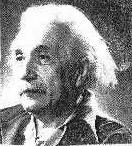
\includegraphics[width=3ex]{figsGeneric/Einstein.jpg}
\vspace{0ex}}
\hspace{0ex} 
}

\newcommand{\Einstein}{
\parbox{7mm}{\vspace{2mm}
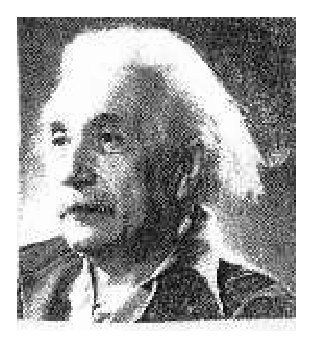
\includegraphics[width=10mm]{figsGeneric/Einstein.eps}
\vspace{-3mm}}\vspace{-3mm}
\hspace{2mm} 
}

\newcommand{\EinsteinLarge}{
\parbox{15mm}{\vspace{2mm}
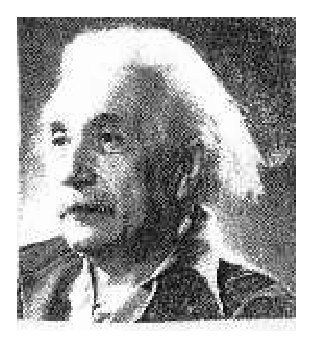
\includegraphics[width=18mm]{figsGeneric/Einstein.eps}
\vspace{-2mm}}\vspace{-2mm}
\hspace{2mm} 
}



\providecommand{\EinsteinBeg}{
\vspace{-3mm}

\Einstein
\vspace{3mm}

}

\providecommand{\simulate}{
  \parbox{0.22\textwidth}{
    \figSimple{0.08\textwidth}
      {$HOME/tex/inputs/figsGeneric/trafficSimulationDe-ring.png}
    \\[-0.06\textwidth]
    \hspace*{0.08\textwidth} \greenSim{%\boldmath{$\Rightarrow$}
      \footnotesize{\textbf{simulate ...}}}
}}

\newcommand{\treiber}{\ \includegraphics[height=1.6em]
   {$HOME/tex/inputs/figsGeneric/signMT_blue.jpg}}
\newcommand{\treiberEps}{\ \includegraphics[height=1.6em]
   {$HOME/tex/inputs/figsGeneric/signMT_blue.eps}}



\newcommand{\OK}{\ 
\includegraphics[width=1.2em]
   {$HOME/tex/inputs/figsGeneric/OK.png}}
\newcommand{\OKeps}{
\includegraphics[width=1.2em]
   {$HOME/tex/inputs/figsGeneric/OK.eps}}

\newcommand{\contradiction}{
  \parbox{1.2em}{\vspace*{-0.2em}
  
\includegraphics[width=0.9em, origin=br]
   {$HOME/tex/inputs/figsGeneric/contradiction.png}\vspace*{0.2em}}
}

\newcommand{\contradictioneps}{
  \parbox{1.2em}{\vspace*{-0.2em}
  
\includegraphics[width=0.9em, origin=br]
   {$HOME/tex/inputs/figsGeneric/contradiction.eps}\vspace*{0.2em}}
}

\newcommand{\false}{\text{{\Large\red{\bfmath{\!\!\times}}}}}

\newcommand{\male}{
\includegraphics[height=1em]
   {$HOME/tex/inputs/figsGeneric/male.eps}}
\newcommand{\female}{
\includegraphics[height=1em]
   {$HOME/tex/inputs/figsGeneric/female.eps}}

\newcommand{\malepng}{
\includegraphics[height=1em]
   {$HOME/tex/inputs/figsGeneric/male.png}}
\newcommand{\femalepng}{
\includegraphics[height=1em]
   {$HOME/tex/inputs/figsGeneric/female.png}}

\newcommand{\circlei}{
  \parbox{1.2em}{\vspace*{-0.2em}
  
\includegraphics[width=1.2em, origin=br]
   {$HOME/tex/inputs/figsGeneric/1circle.eps}\vspace*{0.2em}}
}

\newcommand{\circleii}{
  \parbox{1.2em}{\vspace*{-0.2em}
  
\includegraphics[width=1.2em, origin=br]
   {$HOME/tex/inputs/figsGeneric/2circle.eps}\vspace*{0.2em}}
}

\newcommand{\circleiii}{
  \parbox{1.2em}{\vspace*{-0.2em}
  
\includegraphics[width=1.2em, origin=br]
   {$HOME/tex/inputs/figsGeneric/3circle.eps}\vspace*{0.2em}}
}

\newcommand{\circleiv}{
  \parbox{1.2em}{\vspace*{-0.2em}
  
\includegraphics[width=1.2em, origin=br]
   {$HOME/tex/inputs/figsGeneric/4circle.eps}\vspace*{0.2em}}
}

\newcommand{\circlev}{
  \parbox{1.2em}{\vspace*{-0.2em}
  
\includegraphics[width=1.2em, origin=br]
   {$HOME/tex/inputs/figsGeneric/5circle.eps}\vspace*{0.2em}}
}


%******************************************************************
% General defs for tables
%******************************************************************

\providecommand{\titlebox}[1]{\parbox{140mm}{\vspace{2mm} #1 \vspace{2mm}}}

% top/bottom lines of the tables too close
\providecommand{\spacelinebot}[1]{\parbox[t]{1mm}{\hspace{1mm}\vspace{#1}}}
\providecommand{\spacelinetop}[1]{\parbox[b]{1mm}{\hspace{1mm}\vspace{#1}}}
\providecommand{\spacelinemid}[1]{\parbox[c]{1mm}{\hspace{1mm}\vspace{#1}}}
\providecommand{\spacingbot}{\parbox[t]{1mm}{\hspace{1mm}\vspace{3mm}}}
\providecommand{\spacingtop}{\parbox[b]{1mm}{\hspace{1mm}\vspace{6mm}}}
\providecommand{\spacingmid}{\parbox[c]{1mm}{\hspace{1mm}\vspace{9mm}}}



%******************************************************************
% General defs for figures                                        *
%******************************************************************

\providecommand{\icon}[1]{
  \parbox{7mm}{\vspace{2mm}
    \includegraphics[width=7mm]{#1}
    \vspace{-3mm}
  }
  \vspace{-3mm}
\hspace{1mm} }

% ex: \fig{0.9\textwidth}{epsfile}
\providecommand{\fig}[2]{
   \begin{center}
     \includegraphics[width=#1]{#2}
   \end{center}
}
\providecommand{\figSimple}[2]{
     \includegraphics[width=#1]{#2}
}

% ex: \figBox{0.9\textwidth}{epsfile}
% figure with parbox; necessary to make horizontal placement of figures/text
% without latex bugs
\providecommand{\figBox}[2]{
  \parbox{#1}{
     \begin{center}
     \includegraphics[width=#1]{#2}
    \end{center}
  }
}

% ex: \figBox{0.9\textwidth}{epsfile}{text}

\providecommand{\figBoxText}[3]{
  \parbox{#1}{
     \begin{center}
     \includegraphics[width=#1]{#2}
     \end{center}
     #3
  }
}

\providecommand{\oldfigc}[2]{
   \renewcommand{\baselinestretch}{1.0}
   \parbox[t]{#1}{\sloppy \small #2}
   \renewcommand{\baselinestretch}{\usualstretch}
   \small \normalsize
   }


% ex: \figps{110mm}{psfile}

\providecommand{\figps}[2]{
   \begin{minipage}[]{#1}
       \epsfxsize #1
       \epsffile{#2}
   \end{minipage}
   }

\providecommand{\figcaption}[3]{
   \renewcommand{\baselinestretch}{1.0} 
   \noindent
   \parbox[]{#1}
      {\sloppy \small Figure #2 \ 
       #3
       }
    \renewcommand{\baselinestretch}{\usualstretch}
    \small \normalsize
   }

% ex: \largefig{filename}{5mm}{\label}{captiontext}

\providecommand{\largefig}[4]{    % left fig, right text
   \begin{minipage}{\lenxtot}
       \figps{\lenxtot}{#1}
       \vspace{#2} \\
       \figcaption{\lenxtot}{#3}{#4}
   \end{minipage}
   }

% ex: \smallfig{\lenxa}{filename}{\lenxb}{\label}{captiontext}

\providecommand{\smallfig}[5]{    % left fig, right text
   \begin{minipage}{\lenxtot}
       \begin{minipage}{#1}
         \figps{#1}{#2}
       \end{minipage}
       \hfill
       \begin{minipage}{#3}
         \figcaption{#3}{#4}{#5}
       \end{minipage}
   \end{minipage}
   }


%******************************************************************
% General macros for math expressions                             *
%******************************************************************

\providecommand{\Int}{\int\limits}
\providecommand{\Sum}{\sum\limits}

\providecommand{\bfall}\textbf{\boldmath } % usual text AND math (after$)
\providecommand{\bfmath}[1]{\mbox{\textbf\boldmath{$#1$}}} % italics+fett!
\providecommand{\fett}\textbf{\boldmath } % usual text AND math (after$)

\providecommand{\dd}{{\textrm d}} %example \dd f/\dd x
\providecommand{\diff}[1]{ \ {\textrm d} #1 \, } % dx: differential operator d roman!
\providecommand{\dif}{\mathrm d} %example \dif f/\dif x
\providecommand{\e}{\mathrm e}   % example: \e^x
%!! Achtung: part, dp etc alles reservierte Befehle!!
\providecommand{\ablpart}[2]{\frac{\partial #1}{\partial #2}}  %d(#1)/d(#2)
\providecommand{\abl}[2]   {\frac{{\textrm d} #1}{{\textrm d} #2}}  % =\abltot
\providecommand{\abltot}[2]{\frac{{\textrm d} #1}{{\textrm d} #2}}  % d(#1)/d(#2)
\providecommand{\ablpartzwei}[2]{\frac{\partial^{2} #1}{\partial #2^{2}}} 
\providecommand{\ablparttwo}[2]{\frac{\partial^{2} #1}{\partial #2^{2}}} 
\providecommand{\ablpartmix}[3]{\frac{\partial^{2} #1}
           {\partial  #2 \ \partial #3}}
\providecommand{\ablpartmixed}[3]{\frac{\partial^{2} #1}
           {\partial  #2 \ \partial #3}}
\providecommand{\ablzwei}[2]{\frac{{\textrm d}^{2} #1}{{\textrm d} #2^{2}}} 

\providecommand{\cc}{^{\ast}}         %konj. komplex 
\providecommand{\complex}{C \hspace*{-0.65 em}
   \parbox{3mm}{\vspace*{-0.2 em} {\scriptsize /}}
    }
\providecommand{\cov}{\mbox{cov}}
\providecommand{\Cov}{\mbox{Cov}} %gross Cov!

\renewcommand{\d}[1]{\partial_{#1}}              %Diff.-operator
\providecommand{\deltat}{\mbox{$\delta(t-t')$}}
\providecommand{\deltar}{\mbox{$\delta(\v{r}-\v{r'})$}}
\providecommand{\deltax}{\mbox{$\delta(x-x')$}}
\providecommand{\deltavx}{\mbox{$\delta(\v{x}-\v{x}')$}}
\providecommand{\deltay}{\mbox{$\delta(y-y')$}}
\providecommand{\deltaz}{\mbox{$\delta(z-z')$}}
\providecommand{\deltart}{\mbox{$\delta(\v{r}-\v{r'})\delta(t-t')$}}
\providecommand{\deltaxyt}{\mbox{$\delta(x-x')\delta(y-y')\delta(t-t')$}}
\providecommand{\deltaij}{\mbox{$\delta_{ij}$}}
\providecommand{\deltaik}{\mbox{$\delta_{ik}$}}
\providecommand{\deltail}{\mbox{$\delta_{il}$}}
\providecommand{\deltajk}{\mbox{$\delta_{jk}$}}
\providecommand{\deltajl}{\mbox{$\delta_{jl}$}}
%arne klappt nicht:
%\providecommand{\dfrac}[2]{{\displaystyle \frac{#1}{#2}}}
\providecommand{\dsumi}{{\displaystyle \sum\limits_{i=1}^{n}}} %Summe im D-stil
\providecommand{\dint}[2]{{\displaystyle\int\limits_{#1}^{#2}}}
\providecommand{\dsum}[2]{{\displaystyle \sum\limits_{#1}^{#2}}}
\providecommand{\dsuml}[2]{{\displaystyle \sum\limits_{#1}^{#2}}} %Summe im D-stil
%\providecommand{\erw}[1]{\mbox{$\left \langle #1 \right \rangle$}} %Erwartungswert
\providecommand{\erw}[1]{\mbox{$E \left( #1 \right )$}} %Erwartungswert
\providecommand{\erf}[1]{\ \mbox{erf} \ #1} %Error function
\providecommand{\floor}[1]{{\textrm floor}\left(#1\right)}
\providecommand{\funkint}[1]{\int \!\!\cal{D}[#1]}
\providecommand{\hc}{^{\dagger}}         %konj. komplex 
\renewcommand{\Im}{\mbox{Im}}                  
\providecommand{\intd}[1]{\int \!d#1}
\providecommand{\intdn}[1]{\int \!\!d^{n}\v{#1}}
\providecommand{\intvol}{\int \!\!d^{3}} %keine Zahlen (d3) moegl.
\providecommand{\intvolr}{\int \!\!d^{3} r} %keine Zahlen (d3) moegl.
%\providecommand{\le}{\stackrel{<}{=}}   % less or equal
 
\providecommand{\nab}{\v{\nabla}}
\providecommand{\order}[1]{{\cal O}(#1)}
\providecommand{\overdot}[1]{\stackrel{.}{#1}}        
\renewcommand{\Re}{\mbox{Re}}                      
\providecommand{\re}{\mbox{Re}}                       
\providecommand{\rot}[1]{\v{\nabla}\times \v{#1}}
\providecommand{\sigeps}{\sigma_{\epsilon}}
\providecommand{\hatbeta}{\hat{\beta}}
\providecommand{\hatvec}[1]{\hat{\vec{#1}}}
\providecommand{\vecbeta}{\vec{\beta}}
\providecommand{\bfbeta}{\bfmath{\beta}}
\providecommand{\tilvecx}{\tilde{\vec{x}}}
\providecommand{\tilx}{\tilde{x}}
\providecommand{\hatvecbeta}{\hat{\vec{\beta}}}
\providecommand{\hatsigeps}{\hat{\sigma}_{\epsilon}}
\providecommand{\veceps}{\vec{\epsilon}}
\providecommand{\hatveceps}{\hat{\vec{\epsilon}}}
\providecommand{\hatsigy}{\hat{\sigma}_{y}}
\providecommand{\hatsig}{\hat{\sigma}}
\providecommand{\sumi}{\sum_{i=1}^n}
\renewcommand{\theta}{\vartheta} % zwei Arten von kleinen Thetas, ich
                                % will eins

\providecommand{\sub}[1]{dummy}
\providecommand{\sup}[1]{dummy}
\renewcommand{\sub}[1]{_{\!\!\text{\scriptsize{#1}}}} % recommended \mathrm does not
                                % work for \sub{\"OV} etc
\renewcommand{\sup}[1]{^{\!\!\text{\scriptsize{#1}}}}
%\providecommand{\tr}{^{\!\text{\scriptsize{T}}}}
\providecommand{\tr}{'}
\providecommand{\ueber}[2]{
  \left(\begin{array}{c}
     #1  \\ #2
  \end{array} \right)
}
\providecommand{\tilL}{\tilde{L}}



%\renewcommand{\vec}[1]{\mathbf{#1}}
\renewcommand{\vec}[1]{\text{\boldmath{$#1$}} }
\renewcommand{\bfmath}[1]{\text{\boldmath{$#1$}} }


%\renewcommand{\v}[1]{\mbox{\boldmath$#1$}}     %Vektor = fett
\renewcommand{\v}[1]{\vec{#1}}  %Vektorpfeil/fett je nach obigem renewcommand
%\renewcommand{\v}[1]{\bbox{#1}}     %Vektor = fett, revtex
%\renewcommand{\v}[1]{\underline{#1}} %Vektor = unterstrichen
\providecommand{\vscript}[1]{\mbox{{\scriptsize $\textbf #1$}}} % NOT for greek!


%\providecommand{\m}[1]{\underline{\v{#1}}}                  %Matrix
%\providecommand{\m}[1]{\underline{\underline{#1}}}           %Matrix
\providecommand{\m}[1]{\textbf{\textsf{#1}}\, } %Matrix=fett+gerade(nicht gr)
\providecommand{\mgr}[1]{\text{\boldmath {$#1$}}}  %Matrix griech. \sigma etc


\providecommand{\varabl}[2]{\frac{\delta #1}{\delta #2}}  %d(#1)/d(#2)

%******************************************************************
%      Independent vars etc.                                      *
%******************************************************************
 

\providecommand{\vonx} {\mbox{$(\v{x})$}}                   %(x)
\providecommand{\vonk} {\mbox{$(\v{k})$}}                   %(k)
\providecommand{\vonw} {\mbox{$(\omega )$}}                   %(omega)
\providecommand{\vonr} {\mbox{$(\v{r})$}}                   %(r)
\providecommand{\vonrs} {\mbox{$(\v{r'})$}}                   %(r')
\providecommand{\vonxyt} {\mbox{$(x,y,t)$}}                   %(x,y,z)
\providecommand{\vongrad} {\mbox{$(\v{\nabla })$}}            %(nabla)
\providecommand{\vonrgrad} {\mbox{$(\v{r},\v{\nabla })$}}     %(r,nabla)
\providecommand{\vonxt} {\mbox{$(\v{x},t)$}}                %(x,t)
\providecommand{\vonrt} {\mbox{$(\v{r},t)$}}                %(r,t)
\providecommand{\vonrsts} {\mbox{$(\v{r'},t')$}}                %(r',t')

%******************************************************************
% Misc.                                                           *
%******************************************************************
\providecommand{\nonu} {\nonumber}
\providecommand{\uu}[1]{\underline{\underline{#1}}} 
\providecommand{\COii}{\text{CO}$_2$}


%******************************************************************
% End general defs                                                *
%******************************************************************




%%% Local Variables: 
%%% mode: latex
%%% TeX-master: t
%%% End: 



%###################################################################
% Graphik ACHTUNG [pdftex,dvips] wichtig, sonst Skalierungsbugs bei pdflatex
%###################################################################
%\usepackage[pdftex,dvips]{graphicx} 
%\usepackage[pdftex,dvips]{color}     %Definiert \definecolor und 
                              % red,yellow,green,blue,black,gray,white
\usepackage{graphicx} 
\usepackage{color}
\usepackage{enumitem} % then \begin{enumerate}[(\roman*)] etc possible

%#####################################################
% Hyperlink
%#####################################################
\usepackage{units} %\unit[3]{m/s^2} => 3 m/s^2 etc!
\usepackage{eurosym}  %Euro-Symbol: \euro{Zahl} oder euro{}

%implements blocks: \begin{addmargin}[1em]{0em}% 1em left, 2em right
\usepackage{scrextend} 

\usepackage{hyperref}
% nternet-Link: \href{http://www.WasAuchImmer.html}
% {\blue{\underline{TextDesLinks} }}
% Lokaler Link: \hyperlink{targetName}{TextDesLinks}
% Link-Target: \hypertarget{targetName}

% Lokale Links: mark target with e.g. 
% \hypertarget{fig:IDM}{Target mit label fig:IDM}
% and link to it with \myLocalLink{fig:IDM}{Link zu Target fig:IDM}
\providecommand{\myHyperlink}[2]{\href{#1}{\blue{\underline{#2}}}}
\providecommand{\myLocalLink}[2]{\hyperlink{#1}{\blue{\underline{#2}}}}

%###################################################################
% bibliography-hack to put citation in my order and at several places
%###################################################################

% * need name-oriented citation style such that citation 
%   can be attributed, e.g., \bibliographystyle{elsarticle-harv}

% * compile normally with bibtex and enter resulting .bbl file
%   manually at appropriate places (commenting out bib commands)

% * remove \bibliography{...} and compile ONCE (at the second time, we
% get ?? in the citation places)

\newcommand{\mybibentry}[1]{
\parindent0em
\hspace{2em}
\parbox{0.95\textwidth}{
\parindent-2em
#1
\vspace{1ex}
}

}


% use no-link generation for cite and citep because they are broken
% as a side effect

\newcommand*{\nolinkcite}[1]{%
  {\protect\NoHyper\cite{#1}\protect\endNoHyper}%
}
\newcommand*{\nolinkcitep}[1]{%
  {\protect\NoHyper\citep{#1}\protect\endNoHyper}%
}

% end bibliography-hack to put citation in my citation order 
% and at several places
%########################################################


%#####################################################
% Preprint vs. Publikation
%#####################################################
\providecommand{\martin}[1]{\green{Martin: #1}} %Preprint
%\providecommand{\martin}[1]{}                  %fuer Veroeffentlichung
\providecommand{\arne}[1]{\green{Martin: #1}}   %Preprint
%\providecommand{\arne}[1]{}                    %fuer Veroeffentlichung


%#####################################################
% latest changes from Arne
%#####################################################

% 8-10-04: ex: \includefig{110mm}{psfile}
\newcommand{\includefig}[2]{\includegraphics[width=#1]{#2}}
\providecommand{\bra}{\langle}
\providecommand{\ket}{\rangle}
%#####################################################
% defs of Arne
%#####################################################

\providecommand{\uul}{\uu}
\providecommand{\ug}{\approx}  % ungefaehr gleich
\providecommand{\nor}[1]{\mathrm{#1}}
\providecommand{\sollsein}{\,{\stackrel{!}{=}}\,}
\providecommand{\binom}[2]{\ueber{#1}{#2}}
\providecommand{\www}[1]{\texttt{#1}}
\providecommand{\mytilde}{\symbol{126}} % ist die Tilde!!!
\providecommand{\etal}{\textit{et al.}}
%
\providecommand{\cl}[1]{{\centering #1}}
\providecommand{\no}{\noindent}  % keine Einr�ckung bei neuer Zeile
%
\providecommand{\bno}{\begin{equation*}}   % no citation number
\providecommand{\eno}{\end{equation*}}

\providecommand{\also}{$\to\,$}
\providecommand{\kasten}[1]{\begin{displaymath}\fbox{$\quad\displaystyle #1\quad$}\end{displaymath}}
\providecommand{\ul}[1]{\underline{#1}}   
\providecommand{\uu}[1]{\underline{\underline{#1}}}  % bereits in latex def!
\providecommand{\uul}{\uu}
\providecommand{\ol}[1]{\overline{#1}} 
%fuer mich:
%irgendwie mit german schon definiert !?
\providecommand{\3}{{\ss }}



%******************************************************************
%  General definitions for latex, revtex
%******************************************************************
\renewcommand{\ae}{{\"a}\hspace{-0.4em}}
\renewcommand{\oe}{{\"o}\hspace{-0.4em}}
\providecommand{\ue}{{\"u}\hspace{-0.4em}}
\providecommand{\Ae}{{\"A}\hspace{-0.4em}}
\providecommand{\Oe}{{\"O}\hspace{-0.4em}}
\providecommand{\Ue}{{\"U}\hspace{-0.4em}}


% to circumvent a bug that euro symbols are not displayed in math mode
\providecommand{\eur}{\text{\euro{}}}


\providecommand{\IR}{I\!\!R}
\providecommand{\IN}{I\!\!N}

\providecommand{\lowtilde}{{\mbox{$_{\tilde{}}$}}}
\providecommand{\backsl}{\mbox{$\backslash\!$}}




%##################################################
% colors
%##################################################

% defines {\black ...}, {\red ...}, ... and
%\black{} \red{} \green{} \turk{} \viol{} \orange{}
% \brown{} \grey{}
% visible only in ps not in dvi! (=>tex2ps <texfile w/o ext>)

%\usepackage[dvips]{color} %!! sometimes ``option clash''=> def w/o options
\usepackage{color}

\definecolor{black}{rgb}{0,0,0}
\definecolor{red}{rgb}{0.8,0,0}
\definecolor{lightred}{rgb}{1,0.5,0.5}
\definecolor{green}{rgb}{0,0.8,0}
\definecolor{blue}{rgb}{0,0,1}
\definecolor{turk}{rgb}{0,1,1}
\definecolor{viol}{rgb}{1,0,1}
\definecolor{orange}{rgb}{1,0.4,0.}
\definecolor{yellow}{rgb}{1,0.7,0.}
\definecolor{brown}{rgb}{0.7,0.4,0}
\definecolor{gray}{rgb}{0.7,0.7,0.7}
\definecolor{darkgray}{rgb}{0.5,0.5,0.5}
\definecolor{lightgray}{rgb}{0.95,0.95,1.0}
\definecolor{verylightred}{rgb}{1,0.7,0.5}

\definecolor{TUDblue1}{rgb}{.05,.22,.410}
\definecolor{TUDblue2}{rgb}{.11, .42, .81}
\definecolor{green2}{rgb}{0.,0.7,0.1}
\definecolor{greenSim}{rgb}{0.2,0.4,0.0}
\definecolor{mygreen}{rgb}{0.,0.4,0.4}
\definecolor{myred}{rgb}{1,0.0,0.0}
\definecolor{blueTUD}{rgb}{0.1,0,0.5} 

%% !! only so cumbersome. Short search: 
% No shortcut defining rgb directly (nov19)

\providecommand{\verylightred}[1]{\textcolor{verylightred}{#1}}
\providecommand{\black}[1]{\textcolor{black}{#1}}
\providecommand{\red}[1]{\textcolor{red}{#1}}
\providecommand{\blue}[1]{\textcolor{blue}{#1}}
\providecommand{\green}[1]{\textcolor{green}{#1}}
\providecommand{\turk}[1]{\textcolor{turk}{#1}}
\providecommand{\viol}[1]{\textcolor{viol}{#1}}
\providecommand{\orange}[1]{\textcolor{orange}{#1}}
\providecommand{\yellow}[1]{\textcolor{yellow}{#1}}
\providecommand{\brown}[1]{\textcolor{brown}{#1}}
\providecommand{\gray}[1]{\textcolor{gray}{#1}}
\providecommand{\lightgray}[1]{\textcolor{lightgray}{#1}}
\providecommand{\lightred}[1]{\textcolor{lightred}{#1}}

\newcommand{\myred}[1]{{\color{myred} #1}}
\newcommand{\myblue}[1]{{\color{TUDblue1} #1}}
\newcommand{\mygreen}[1]{{\color{mygreen} #1}}
\newcommand{\greenSim}[1]{{\color{greenSim} #1}}
\newcommand{\darkgreen}[1]{{\color{green2} #1}} %green2 in command,
                                                %not in def, error
\newcommand{\blueTUD}[1]{{\color{blueTUD} #1}}  %my color
\providecommand{\bfblueTUD}[1]{\hspace*{0.01em}{\boldmath \textbf{\blueTUD{#1}}}}
\providecommand{\bfblack}[1]{\hspace*{0.01em}{\boldmath \textbf{\black{ #1}}}}
\providecommand{\bfgreen}[1]{\hspace*{0.01em}{\boldmath \textbf{\green{#1}}}}
\providecommand{\bfred}  [1]{\hspace*{0.01em}{\boldmath \textbf{\red{#1}}}}
\providecommand{\bfblue}  [1]{\hspace*{0.01em}{\boldmath \textbf{\blue{#1}}}}
\providecommand{\bforange}[1]{\hspace*{0.01em}{\boldmath
    \textbf{\orange{#1}}}}
\providecommand{\bfyellow}[1]{\hspace*{0.01em}{\boldmath 
    \textbf{\yellow{#1}}}} 



%#################################################################
% special colors definitions for special structures in scripts/transparencies
%#################################################################

% main text
\definecolor{colMainText}{rgb}{1,0.75,0.3}
\newcommand{\colMainText}[1]{{\color{colMainText} #1}}

% main equations
\definecolor{colMainEq}{rgb}{1,0.75,0.3}
\newcommand{\colMainEq}[1]{{\color{colMainEq} #1}}


% definitions
\definecolor{colDef}{rgb}{0.6,0,0.2}
\newcommand{\colDef}[1]{{\color{colDef} #1}}
\providecommand{\bfdef}[1]{\hspace*{0.01em}{\boldmath \textbf{\colDef{#1}}}}

% questions and answers

\definecolor{colAsk}{rgb}{1,0.5,0.}
\newcommand{\colAsk}[1]{{\color{colAsk} #1}}

\definecolor{colAnswer}{rgb}{0,0.5,0.5}
\newcommand{\colAnswer}[1]{{\color{colAnswer} #1}}

\providecommand{\bfAsk}[1]{\hspace*{0.01em}{\boldmath \textbf{\colAsk{#1}}}}
\providecommand{\bfAnswer}[1]{\hspace*{0.01em}{\boldmath
    \textbf{\colAnswer{#1}}}}

\providecommand{\itemAsk}{\item[\bfAsk{?\ }]}
\providecommand{\itemAnswer}{\item[\bfAnswer{!\ }]}

% comments before '=' signs in calculation steps
% example: 
% \bdma S &=& (AB)C \\ \remark{associativity} &=& ABC \edma
\providecommand{\remark}[1]{\text{\scriptsize{\red{[#1 $\to$]}}}}

%#################################################################

\newcommand{\rlogo}[1]{\hfill {\color{black} {\texttt{#1.}}} \hspace*{-3mm} \includegraphics[width=4mm]{../style/Rlogo}}

%###########################################################
% absolute positioning of boxes or images
%###########################################################


% https://tex.stackexchange.com/questions/311007/change-package-option-overlay-from-textpos-package-in-document/311031#311031

\usepackage{tikz}
\usetikzlibrary{calc}
\newcommand{\placebox}[4][center]{%
  % [#1]: box anchor: center (default) | 
  %                 south west | west | north west | north |
  %                 north east | east | south east | south | 
  %                 mid west | mid | mid east |
  %                 base west | base | base east 
  % #2: horizontal position (fraction of page width)
  % #3: vertical position (fraction of page height)
  % #4: content
  %
  \tikz[remember picture,overlay,x=\paperwidth,y=\paperheight]{%
    \node[anchor=#1,inner sep=0pt]
    at ($(current page.south west)+(#2,#3)$) {#4};
  }%
}
%###########################################################

% make images pale (see demo_makePale.tex) transparency cover
%\makePale{opacity}{centerXrel}{centerYrel}{wrel}{hrel}
% e.g., \makePale{0.6}{0.5}{0.5}{1}{0.3}

\usepackage{pgfcore}

\providecommand{\makePale}[5]{
 \setlength{\unitlength}{0.5\textwidth}
 \placebox{#2}{#3}{
   \begin{picture}(0,0)
   \put(-#4,-#5){
    \pgfsetfillopacity{#1}{
     \textcolor{white}{\rule{#4\textwidth}{#5\textheight}}
    }
   }
   \end{picture}
 }
}

%###########################################################



%usage \circled{2} gives 2 in a circle

\newcommand*\circled[1]{\tikz[baseline=(char.base)]{
    \node[shape=circle, draw, inner sep=1pt, 
        minimum height=12pt] (char) {#1};}}





% example own definition
\definecolor{lyellow}{rgb}{1,1,0.5}
\providecommand{\lyellow}[1]{\textcolor{lyellow}{#1}}
\definecolor{lblue}{rgb}{0.91,1,1}
\providecommand{\lblue}[1]{\textcolor{lblue}{#1}}

% find keywords: caption, title
\providecommand{\bfsf}[1]{\large{\sffamily\textbf{#1}}}
\providecommand{\secfont}[1]{\Large{\sffamily\textbf{#1}}}
\providecommand{\myheading}[1]{\Large{\sffamily\textbf{\blueTUD{#1}}}}
\providecommand{\mysubheading}[1]{\large{\sffamily\textbf{\blueTUD{#1}}}}
\providecommand{\mysubsubheading}[1]{\sffamily\textbf{\blueTUD{#1}}}

\providecommand{\white}[1]{\textcolor{white}{#1}}
\providecommand{\myheadingWhite}[1]{\Large{\sffamily\textbf{\white{#1}}}}
\providecommand{\mysubheadingWhite}[1]{\large{\sffamily\textbf{\white{#1}}}}

%******************************************************************
% General defs for structural units and environments 
%******************************************************************

% see also \mysubheading etc

\providecommand{\mysection}[1]   {\section{{\textsf\Large\textbf{#1}}}}
\providecommand{\mysubsection}[1]{\subsection{{\textsf\large\textbf{#1}}}}

% fuer usepackage[a4paper]{foils}  (sonst Headings groe\3er)
%calling sequence: \myfigure{title}{images}{explanatory text}
\providecommand{\myfigure}[3]{
%\newpage
\begin{center}
{\large\textsf\textbf{#1}} \\[-4mm]
\end{center}
#2

#3
}


\providecommand{\bc}{\begin{center}}
\providecommand{\ec}{\end{center}}
\providecommand{\be}{\begin{equation}}
\providecommand{\ee}{\end{equation}}
\providecommand{\bea}{\begin{eqnarray}}
\providecommand{\eea}{\end{eqnarray}}
\providecommand{\bdm}{\begin{displaymath}}
\providecommand{\edm}{\end{displaymath}}
\providecommand{\bdma}{\begin{eqnarray*}}
\providecommand{\edma}{\end{eqnarray*}}
\providecommand{\ba}{\begin{eqnarray*}}
\providecommand{\ea}{\end{eqnarray*}}
\providecommand{\bi}{\begin{itemize}}
\providecommand{\ei}{\end{itemize}}
\providecommand{\benum}{\begin{enumerate}}
\providecommand{\eenum}{\end{enumerate}}
%F...ing new bug in beamer class: enum label not defined=> infinite loop
% providecommand => only used if undefined
\providecommand{\labelenumi}{\arabic*.}     %# 1st level
\providecommand{\labelenumii}{(\alph*)}    %# 2nd level
\providecommand{\labelenumiii}{(\Roman*)}  %# 3rd level
\providecommand{\labelenumiv}{(\roman*)}   %# 4th level (Greek not defined)

\providecommand{\dis}[1]{ {\displaystyle #1}}

%example:\dmTwo{qlhs1 &=rhs1 \\ lhs2 &=rhs2}
\providecommand{\dmTwo}[1]{
  \begin{displaymath}
    \begin{array}{ll} #1
    \end{array}
  \end{displaymath}
}
% wie bdma ... edma, aber alles linkszentriert

\providecommand{\dmThree}[1]{
  \begin{displaymath}
    \begin{array}{lll} #1
    \end{array}
  \end{displaymath}
}

%example: $ f(x)=\twoCases{0}{x<0}{1}{x\ge 0}$
\providecommand{\twoCases}[4]{
  \left\{ 
    \begin{array}{ll} 
      #1 & #2 \\
      #3 & #4 
    \end{array} 
  \right.
}
\providecommand{\threeCases}[6]{
  \left\{ 
    \begin{array}{ll} 
      #1 & #2 \\
      #3 & #4 \\ 
      #5 & #6 
    \end{array} 
  \right.
}
\providecommand{\fourCases}[8]{
  \left\{ 
    \begin{array}{ll} 
      #1 & #2 \\
      #3 & #4 \\ 
      #5 & #6 \\ 
      #7 & #8 
    \end{array} 
  \right.
}

% column vector with parentheses, e.g.,
%\myVector{1\\2\\3}

\providecommand{\myVector}[1]{
  \left(\begin{array}{c} 
      #1 
   \end{array} \right)
}

%matrix with two columns, e.g.,
% \myMatrixTwo{c11&c12\\c21&c22\\c31&c32}
%BESSER: \begin{pmatrix} c11&c12\\c21&c22\end{pmatrix}

\providecommand{\myMatrixTwo}[1]{
  \left(\begin{array}{cc} 
      #1 
   \end{array} \right)
}

%matrix with three columns, e.g.,
% \myMatrixThree{c11&c12&c13\\c21&c22&c23\\c31&c32&c33}
%BESSER: \begin{pmatrix} c11&c12\\c21&c22\end{pmatrix}

\providecommand{\myMatrixThree}[1]{
  \left(\begin{array}{ccc} 
      #1 
   \end{array} \right)
}

\providecommand{\myMatrixFour}[1]{
  \left(\begin{array}{cccc} 
      #1 
   \end{array} \right)
}

\providecommand{\myMatrixFive}[1]{
  \left(\begin{array}{ccccc} 
      #1 
   \end{array} \right)
}

\providecommand{\non}{\nonumber \\}
\providecommand{\no}{\nonumber}

\providecommand{\refkl}[1]{(\ref{#1})}

%######################################
% boxed displayed equations
%######################################

\providecommand{\fboxdm}[1]{
 \begin{center} \fbox{
   ${\displaystyle \begin{array}{l} #1 \end{array}}$} \end{center}
}

\providecommand{\fboxeq}[1]{
\begin{equation}
 \fbox{${\displaystyle  #1 }$}
\end{equation}
}


\providecommand{\fboxtext}[1]{
  \begin{center} \framebox{
    \begin{minipage}{0.8\textwidth} #1 \end{minipage}
  }
  \end{center}
}

\providecommand{\fitfboxtext}[1]{
  \begin{center} 
    \fbox{{#1}}
  \end{center}
}



%#####################################################
% Numberered equation with background color (including the numbering)
% needs colors.sty; ex.: \bgcoloreq{green}{x^2 = y^2+z^2}
\providecommand{\bgcoloreq}[2]{
  \mbox{\colorbox{#1}{
    \begin{minipage}{\textwidth}
      \begin{equation} #2 \end{equation}
    \end{minipage}
  }}
}

%###################################################
% Numberered equation with background color only behind the formula
% needs colors.sty; ex.: \bgeq{green}{label}{x^2 = y^2+z^2}

\providecommand{\bgeq}[3]{
  \begin{equation}
  \label{#2}
  \colorbox{#1}{$ {\displaystyle #3}$}
  \end{equation}
}

%###################################################
% Displayed equation with background color (over whole width)
% needs colors.sty; ex.: \bgcolordm{red}{x^2=1}
\providecommand{\bgcolordm}[2]{
  \mbox{\colorbox{#1}{
    \begin{minipage}{\textwidth}
       \vspace*{-2ex} % folg. Leerzeile wichtig; vspace nicht woanders...

       \begin{displaymath} #2 \end{displaymath}
       \vspace*{-3.8ex} % folg. Leerzeile wichtig, ... da ignoriert


    \end{minipage}
  }}
}

%###############################################
% Centered equation with background color only behind the formula
% needs colors.sty; ex.: \bgcolormath{red}{x^2=1}
\providecommand{\bgcolormathcenter}[2]{
 \begin{center}
  \colorbox{#1}{${\displaystyle #2}$}
 \end{center}
}

%###############################################
% non-centered displayed equation with background color only behind the formula
% needs colors.sty; ex.: \bgcolormath{red}{x^2=1}
\providecommand{\bgcolormath}[2]{
  \colorbox{#1}{${\displaystyle #2}$}
}


%################################################################
% Standard colored box with some margins and width=whole textwidth
% needs colors.sty; ex.: \widecolorbox{lilablassblau}{bel. Inhalt}
\providecommand{\widecolorbox}[2]{
  \mbox{\colorbox{#1}{
    \hspace*{0.5em}\begin{minipage}{0.94\textwidth}
      \vspace*{1ex}

       #2
       \vspace*{1ex}


    \end{minipage}\hspace*{0.5em}
  }}
}

\providecommand{\widecolorboxExmpl}[2]{
  \mbox{\colorbox{#1}{
    \hspace*{0.5em}\begin{minipage}{0.88\textwidth}
      \vspace*{1ex}

       #2
       \vspace*{1ex}


    \end{minipage}\hspace*{0.5em}
  }}
}

%################################################################
% Standard colored box without margins and width=whole textwidth
% needs colors.sty; ex.: \colbox{lilablassblau}{bel. Inhalt}
% NOTE: much more flexible than usual \colorbox!
\providecommand{\colbox}[2]{
  \mbox{\colorbox{#1}{
    \hspace*{0.1em}\begin{minipage}{\textwidth}
      \vspace*{0ex}

       #2
       \vspace*{0ex}


    \end{minipage}\hspace*{-0.1em}
  }}
}


%######################################
% Non-buggy multiline table entry: a component of entryExample below
% Calling sequence: \myBox{width}{text}
%######################################

\newcommand{\myBox}[2]{
  \hspace{-0.2mm}\parbox{#1}{
      \vspace*{2mm}#2\vspace*{2mm}      
  } \hspace*{-1mm}
}
 
%######################################
% Example: 3-column table with
% non-buggy multiline behaviour of the entries (as in usual latex)
% \begin{tabular}{|l|l|l|}  \hline
% \entryExample{left}{center}{right} \entry{ ....} ...
% \end{tabular}  
%######################################

\providecommand{\entryExample}[3]{
       \hspace{2mm}\parbox{40mm}{\vspace*{2mm}#1\vspace*{2mm}} \hspace*{-2mm}
     & \hspace{2mm}\parbox{30mm}{\vspace*{2mm}#2\vspace*{2mm}} \hspace*{-2mm}
     & \hspace{2mm}\parbox{30mm}{\vspace*{2mm}#3\vspace*{2mm}} \hspace*{-2mm}
                        \\ \hline
                       }


%######################################
% Example table with decimal-point centered entries:

% \usepackage{dcolumn}  % Ausrichtung an Dezimalpunkt
% \begin{tabular}{|D{.}{.}{1}|D{.}{.}{1}|D{.}{.}{1}|} \hline
% \entryDec{left}{center}{right}
% \end{tabular}  
%!! aber auch Bug: vergroessert gewaltsam Tabellen, ohne dass
% andere Nichtzahlenzeilen (Titel) dies ausnutzen koennten!
% => muss diesen Bug mit erhoehten \hspace-Werten in \entry (fuer Titel)
% ausmerzen! (anderes geht nicht!! DOS!
%######################################

\providecommand{\entryDec}[3]{
 &&\\[-4mm]                      % schafft oben mehr Platz
 #1 & #2 & #3 \\[1mm] \hline     % schafft unten mehr Platz 
}                              % ! \vspace{..} unterbr Tab, \\[] nicht!



%!! citebox:Latex-Bug: Setzt nicht kleineren Textabstand bei kleinerer Schrift
% breche laengere Eintraege gewaltsam mit \\[-4mm] um
% Bug 2: vertikaler Abstand des Zitierenden #2 oft falsch; korrigiere mit
% \vspace beim #!-Eintrag!

\providecommand{\citebox}[2]{
  \hspace*{\fill}
  \begin{minipage}{90mm}
  %\renewcommand{\baselinestretch}{1.0}
  \footnotesize {\textsl #1}
  \end{minipage}
  \vspace*{-2mm}

  \hspace*{\fill}{ \scriptsize #2 }
}

\providecommand{\citeboxi}[2]{
  \hspace*{\fill}
  \begin{minipage}{100mm}
  \renewcommand{\baselinestretch}{1.0}
  \footnotesize {\sl #1}
  \vspace*{-3mm}\\
  \hspace*{\fill} #2\\
  \end{minipage}
  }

\providecommand{\footnotespace}[1]{\footnote{\hspace{0.3em}#1}}
\providecommand{\tabsetting}{
              \renewcommand{\baselinestretch}{1.0}\small \normalsize}
\providecommand{\tabspacesetting}[1]{
              \renewcommand{\baselinestretch}{#1}\small \normalsize}


%#########################################################
% Create custom environemnts : Those used for Vkmod.tex 
%#########################################################

% usage: \begin{itemize} ... \itemgray{text} ... \end{itemize}
% beware: \colorbox{lightgray}{  .. } extends only over 1 line!
% triangle: tip up
% triangleright: tip right but not filled
% blacktriangleright: tip right, filled=OK override black by color

\providecommand{\itemgray}[1]{
{\color{darkgray}
  \item[\color{darkgray}\scalebox{0.7}{$\blacktriangleright$}] #1}
}

% usage: \aufgabenbox{caption}{text}
\providecommand{\aufgabenbox}[2]{
  \vspace{3mm}
  {\parindent0mm
  \widecolorbox{lightgray}{
    {\textsf\textbf{#1}} \vspace{3mm}

 #2
  }}
 \vspace{5mm}

}

% usage: \verstaendnisbox{text}

\providecommand{\verstaendnisbox}[1]{
  \vspace{3mm}
  {\parindent0mm
  \widecolorbox{lightgray}{
    \textbf{Verst\"andnisfrage:}\\[-8mm]
    \begin{itemize}
      \item[] #1
    \end{itemize}
  \vspace*{-2mm}
  }}
 \vspace{5mm}

}

\providecommand{\examplebox}[2]{
 \begin{center}
  \vspace{3mm}
  {\parindent0mm
  \widecolorboxExmpl{lblue}{
%  \widecolorboxExmpl{lightgray}{
    \textit{#1}\\[0.5em]
    #2
    \vspace*{0.5em}
    }
  }
  \vspace{1em}
  \end{center}
}


%\providecommand{\verstaendnisbox}[1]{
%  \vspace{5mm}
%  \textbf{Verst\"andnisfrage:}\\[-8mm]
%  \begin{itemize}
%    \item[] #1
%  \end{itemize}
%}

%usage: \maineq{eq_label}{formula}

\providecommand{\maineq}[2]{
 \bgeq{colMainEq}{#1}{#2}
}

%usage: \maindm{formula}

\providecommand{\maindm}[1]{
 \bgcolormathcenter{colMainEq}{#1}
}


\providecommand{\maindmIntext}[1]{
 \bgcolormath{colMainEq}{#1}
}

%usage: \maintextbox{width}{text}

\providecommand{\maintextbox}[2]{
\vspace{0.1em}
\begin{center}
  \colorbox{colMainText}{
   \hspace*{0.1em}
     \parbox{#1}{\vspace*{0.1em}
     #2\vspace*{0.1em}
     }
   \hspace*{0.1em} 
  }
\end{center}
\vspace{0mm}
}

\providecommand{\maintextboxNocenter}[2]{
\vspace{0.1em}
  \colorbox{colMainText}{
   \hspace*{0.1em}
     \parbox{#1}{\vspace*{0.1em}
     #2\vspace*{0.1em}
     }
   \hspace*{0.1em} 
  }
\vspace{0mm}
}

%usage: \maintext{text}

\providecommand{\maintext}[1]{
 \maintextbox{0.95\textwidth}{#1}
}

\providecommand{\maintextSimple}[1]{ % bug: no center allowed in placebox
  \colorbox{colMainText}{
   \hspace*{0.1em}
     \parbox{0.95\textwidth}{\vspace*{0.1em}
     #1\vspace*{0.1em}
     }
   \hspace*{0.1em} 
  }
}


\providecommand{\maintextSimplebox}[2]{ % bug: no center allowed in placebox
\vspace{0.1em}
  \colorbox{colMainText}{
   \hspace*{0.1em}
     \parbox{#1}{\vspace*{0.1em}
     #2\vspace*{0.1em}
     }
   \hspace*{0.1em} 
  }
\vspace{0mm}
}


%******************************************************************
% General defs for words, text symbols and icons
%******************************************************************
\providecommand{\text}[1]{{\mbox{ #1}}}

\providecommand{\Angstroem}{{\AA}}
\providecommand{\cels}{\mbox{$^{\circ}{\textrm C}$}}
\providecommand{\emptySet}{\{\not\hspace{-1mm}0\}}
\providecommand{\Fr}{\mbox{Fr\'{e}edericksz--}}
\providecommand{\Poincare}{Poincar\'{e}}
\providecommand{\rb}{Rayleigh--B\'{e}nard}
\providecommand{\RB}{Rayleigh--B\'{e}nard}
\providecommand{\via}{\textit{via}}
\providecommand{\msii}{\mbox{m/s$^2$}}
\providecommand{\result}[1]{\underline{\underline{#1}}}
 
\newcommand{\EinsteinPdflatex}{
\parbox{3ex}{\vspace{-0ex}
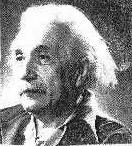
\includegraphics[width=3ex]{figsGeneric/Einstein.jpg}
\vspace{0ex}}
\hspace{0ex} 
}

\newcommand{\Einstein}{
\parbox{7mm}{\vspace{2mm}
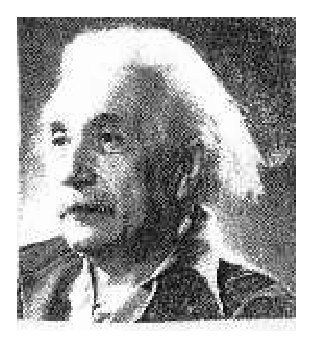
\includegraphics[width=10mm]{figsGeneric/Einstein.eps}
\vspace{-3mm}}\vspace{-3mm}
\hspace{2mm} 
}

\newcommand{\EinsteinLarge}{
\parbox{15mm}{\vspace{2mm}
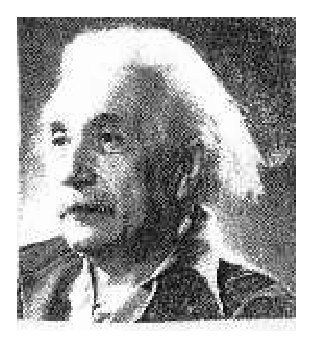
\includegraphics[width=18mm]{figsGeneric/Einstein.eps}
\vspace{-2mm}}\vspace{-2mm}
\hspace{2mm} 
}



\providecommand{\EinsteinBeg}{
\vspace{-3mm}

\Einstein
\vspace{3mm}

}

\providecommand{\simulate}{
  \parbox{0.22\textwidth}{
    \figSimple{0.08\textwidth}
      {$HOME/tex/inputs/figsGeneric/trafficSimulationDe-ring.png}
    \\[-0.06\textwidth]
    \hspace*{0.08\textwidth} \greenSim{%\boldmath{$\Rightarrow$}
      \footnotesize{\textbf{simulate ...}}}
}}

\newcommand{\treiber}{\ \includegraphics[height=1.6em]
   {$HOME/tex/inputs/figsGeneric/signMT_blue.jpg}}
\newcommand{\treiberEps}{\ \includegraphics[height=1.6em]
   {$HOME/tex/inputs/figsGeneric/signMT_blue.eps}}



\newcommand{\OK}{\ 
\includegraphics[width=1.2em]
   {$HOME/tex/inputs/figsGeneric/OK.png}}
\newcommand{\OKeps}{
\includegraphics[width=1.2em]
   {$HOME/tex/inputs/figsGeneric/OK.eps}}

\newcommand{\contradiction}{
  \parbox{1.2em}{\vspace*{-0.2em}
  
\includegraphics[width=0.9em, origin=br]
   {$HOME/tex/inputs/figsGeneric/contradiction.png}\vspace*{0.2em}}
}

\newcommand{\contradictioneps}{
  \parbox{1.2em}{\vspace*{-0.2em}
  
\includegraphics[width=0.9em, origin=br]
   {$HOME/tex/inputs/figsGeneric/contradiction.eps}\vspace*{0.2em}}
}

\newcommand{\false}{\text{{\Large\red{\bfmath{\!\!\times}}}}}

\newcommand{\male}{
\includegraphics[height=1em]
   {$HOME/tex/inputs/figsGeneric/male.eps}}
\newcommand{\female}{
\includegraphics[height=1em]
   {$HOME/tex/inputs/figsGeneric/female.eps}}

\newcommand{\malepng}{
\includegraphics[height=1em]
   {$HOME/tex/inputs/figsGeneric/male.png}}
\newcommand{\femalepng}{
\includegraphics[height=1em]
   {$HOME/tex/inputs/figsGeneric/female.png}}

\newcommand{\circlei}{
  \parbox{1.2em}{\vspace*{-0.2em}
  
\includegraphics[width=1.2em, origin=br]
   {$HOME/tex/inputs/figsGeneric/1circle.eps}\vspace*{0.2em}}
}

\newcommand{\circleii}{
  \parbox{1.2em}{\vspace*{-0.2em}
  
\includegraphics[width=1.2em, origin=br]
   {$HOME/tex/inputs/figsGeneric/2circle.eps}\vspace*{0.2em}}
}

\newcommand{\circleiii}{
  \parbox{1.2em}{\vspace*{-0.2em}
  
\includegraphics[width=1.2em, origin=br]
   {$HOME/tex/inputs/figsGeneric/3circle.eps}\vspace*{0.2em}}
}

\newcommand{\circleiv}{
  \parbox{1.2em}{\vspace*{-0.2em}
  
\includegraphics[width=1.2em, origin=br]
   {$HOME/tex/inputs/figsGeneric/4circle.eps}\vspace*{0.2em}}
}

\newcommand{\circlev}{
  \parbox{1.2em}{\vspace*{-0.2em}
  
\includegraphics[width=1.2em, origin=br]
   {$HOME/tex/inputs/figsGeneric/5circle.eps}\vspace*{0.2em}}
}


%******************************************************************
% General defs for tables
%******************************************************************

\providecommand{\titlebox}[1]{\parbox{140mm}{\vspace{2mm} #1 \vspace{2mm}}}

% top/bottom lines of the tables too close
\providecommand{\spacelinebot}[1]{\parbox[t]{1mm}{\hspace{1mm}\vspace{#1}}}
\providecommand{\spacelinetop}[1]{\parbox[b]{1mm}{\hspace{1mm}\vspace{#1}}}
\providecommand{\spacelinemid}[1]{\parbox[c]{1mm}{\hspace{1mm}\vspace{#1}}}
\providecommand{\spacingbot}{\parbox[t]{1mm}{\hspace{1mm}\vspace{3mm}}}
\providecommand{\spacingtop}{\parbox[b]{1mm}{\hspace{1mm}\vspace{6mm}}}
\providecommand{\spacingmid}{\parbox[c]{1mm}{\hspace{1mm}\vspace{9mm}}}



%******************************************************************
% General defs for figures                                        *
%******************************************************************

\providecommand{\icon}[1]{
  \parbox{7mm}{\vspace{2mm}
    \includegraphics[width=7mm]{#1}
    \vspace{-3mm}
  }
  \vspace{-3mm}
\hspace{1mm} }

% ex: \fig{0.9\textwidth}{epsfile}
\providecommand{\fig}[2]{
   \begin{center}
     \includegraphics[width=#1]{#2}
   \end{center}
}
\providecommand{\figSimple}[2]{
     \includegraphics[width=#1]{#2}
}

% ex: \figBox{0.9\textwidth}{epsfile}
% figure with parbox; necessary to make horizontal placement of figures/text
% without latex bugs
\providecommand{\figBox}[2]{
  \parbox{#1}{
     \begin{center}
     \includegraphics[width=#1]{#2}
    \end{center}
  }
}

% ex: \figBox{0.9\textwidth}{epsfile}{text}

\providecommand{\figBoxText}[3]{
  \parbox{#1}{
     \begin{center}
     \includegraphics[width=#1]{#2}
     \end{center}
     #3
  }
}

\providecommand{\oldfigc}[2]{
   \renewcommand{\baselinestretch}{1.0}
   \parbox[t]{#1}{\sloppy \small #2}
   \renewcommand{\baselinestretch}{\usualstretch}
   \small \normalsize
   }


% ex: \figps{110mm}{psfile}

\providecommand{\figps}[2]{
   \begin{minipage}[]{#1}
       \epsfxsize #1
       \epsffile{#2}
   \end{minipage}
   }

\providecommand{\figcaption}[3]{
   \renewcommand{\baselinestretch}{1.0} 
   \noindent
   \parbox[]{#1}
      {\sloppy \small Figure #2 \ 
       #3
       }
    \renewcommand{\baselinestretch}{\usualstretch}
    \small \normalsize
   }

% ex: \largefig{filename}{5mm}{\label}{captiontext}

\providecommand{\largefig}[4]{    % left fig, right text
   \begin{minipage}{\lenxtot}
       \figps{\lenxtot}{#1}
       \vspace{#2} \\
       \figcaption{\lenxtot}{#3}{#4}
   \end{minipage}
   }

% ex: \smallfig{\lenxa}{filename}{\lenxb}{\label}{captiontext}

\providecommand{\smallfig}[5]{    % left fig, right text
   \begin{minipage}{\lenxtot}
       \begin{minipage}{#1}
         \figps{#1}{#2}
       \end{minipage}
       \hfill
       \begin{minipage}{#3}
         \figcaption{#3}{#4}{#5}
       \end{minipage}
   \end{minipage}
   }


%******************************************************************
% General macros for math expressions                             *
%******************************************************************

\providecommand{\Int}{\int\limits}
\providecommand{\Sum}{\sum\limits}

\providecommand{\bfall}\textbf{\boldmath } % usual text AND math (after$)
\providecommand{\bfmath}[1]{\mbox{\textbf\boldmath{$#1$}}} % italics+fett!
\providecommand{\fett}\textbf{\boldmath } % usual text AND math (after$)

\providecommand{\dd}{{\textrm d}} %example \dd f/\dd x
\providecommand{\diff}[1]{ \ {\textrm d} #1 \, } % dx: differential operator d roman!
\providecommand{\dif}{\mathrm d} %example \dif f/\dif x
\providecommand{\e}{\mathrm e}   % example: \e^x
%!! Achtung: part, dp etc alles reservierte Befehle!!
\providecommand{\ablpart}[2]{\frac{\partial #1}{\partial #2}}  %d(#1)/d(#2)
\providecommand{\abl}[2]   {\frac{{\textrm d} #1}{{\textrm d} #2}}  % =\abltot
\providecommand{\abltot}[2]{\frac{{\textrm d} #1}{{\textrm d} #2}}  % d(#1)/d(#2)
\providecommand{\ablpartzwei}[2]{\frac{\partial^{2} #1}{\partial #2^{2}}} 
\providecommand{\ablparttwo}[2]{\frac{\partial^{2} #1}{\partial #2^{2}}} 
\providecommand{\ablpartmix}[3]{\frac{\partial^{2} #1}
           {\partial  #2 \ \partial #3}}
\providecommand{\ablpartmixed}[3]{\frac{\partial^{2} #1}
           {\partial  #2 \ \partial #3}}
\providecommand{\ablzwei}[2]{\frac{{\textrm d}^{2} #1}{{\textrm d} #2^{2}}} 

\providecommand{\cc}{^{\ast}}         %konj. komplex 
\providecommand{\complex}{C \hspace*{-0.65 em}
   \parbox{3mm}{\vspace*{-0.2 em} {\scriptsize /}}
    }
\providecommand{\cov}{\mbox{cov}}
\providecommand{\Cov}{\mbox{Cov}} %gross Cov!

\renewcommand{\d}[1]{\partial_{#1}}              %Diff.-operator
\providecommand{\deltat}{\mbox{$\delta(t-t')$}}
\providecommand{\deltar}{\mbox{$\delta(\v{r}-\v{r'})$}}
\providecommand{\deltax}{\mbox{$\delta(x-x')$}}
\providecommand{\deltavx}{\mbox{$\delta(\v{x}-\v{x}')$}}
\providecommand{\deltay}{\mbox{$\delta(y-y')$}}
\providecommand{\deltaz}{\mbox{$\delta(z-z')$}}
\providecommand{\deltart}{\mbox{$\delta(\v{r}-\v{r'})\delta(t-t')$}}
\providecommand{\deltaxyt}{\mbox{$\delta(x-x')\delta(y-y')\delta(t-t')$}}
\providecommand{\deltaij}{\mbox{$\delta_{ij}$}}
\providecommand{\deltaik}{\mbox{$\delta_{ik}$}}
\providecommand{\deltail}{\mbox{$\delta_{il}$}}
\providecommand{\deltajk}{\mbox{$\delta_{jk}$}}
\providecommand{\deltajl}{\mbox{$\delta_{jl}$}}
%arne klappt nicht:
%\providecommand{\dfrac}[2]{{\displaystyle \frac{#1}{#2}}}
\providecommand{\dsumi}{{\displaystyle \sum\limits_{i=1}^{n}}} %Summe im D-stil
\providecommand{\dint}[2]{{\displaystyle\int\limits_{#1}^{#2}}}
\providecommand{\dsum}[2]{{\displaystyle \sum\limits_{#1}^{#2}}}
\providecommand{\dsuml}[2]{{\displaystyle \sum\limits_{#1}^{#2}}} %Summe im D-stil
%\providecommand{\erw}[1]{\mbox{$\left \langle #1 \right \rangle$}} %Erwartungswert
\providecommand{\erw}[1]{\mbox{$E \left( #1 \right )$}} %Erwartungswert
\providecommand{\erf}[1]{\ \mbox{erf} \ #1} %Error function
\providecommand{\floor}[1]{{\textrm floor}\left(#1\right)}
\providecommand{\funkint}[1]{\int \!\!\cal{D}[#1]}
\providecommand{\hc}{^{\dagger}}         %konj. komplex 
\renewcommand{\Im}{\mbox{Im}}                  
\providecommand{\intd}[1]{\int \!d#1}
\providecommand{\intdn}[1]{\int \!\!d^{n}\v{#1}}
\providecommand{\intvol}{\int \!\!d^{3}} %keine Zahlen (d3) moegl.
\providecommand{\intvolr}{\int \!\!d^{3} r} %keine Zahlen (d3) moegl.
%\providecommand{\le}{\stackrel{<}{=}}   % less or equal
 
\providecommand{\nab}{\v{\nabla}}
\providecommand{\order}[1]{{\cal O}(#1)}
\providecommand{\overdot}[1]{\stackrel{.}{#1}}        
\renewcommand{\Re}{\mbox{Re}}                      
\providecommand{\re}{\mbox{Re}}                       
\providecommand{\rot}[1]{\v{\nabla}\times \v{#1}}
\providecommand{\sigeps}{\sigma_{\epsilon}}
\providecommand{\hatbeta}{\hat{\beta}}
\providecommand{\hatvec}[1]{\hat{\vec{#1}}}
\providecommand{\vecbeta}{\vec{\beta}}
\providecommand{\bfbeta}{\bfmath{\beta}}
\providecommand{\tilvecx}{\tilde{\vec{x}}}
\providecommand{\tilx}{\tilde{x}}
\providecommand{\hatvecbeta}{\hat{\vec{\beta}}}
\providecommand{\hatsigeps}{\hat{\sigma}_{\epsilon}}
\providecommand{\veceps}{\vec{\epsilon}}
\providecommand{\hatveceps}{\hat{\vec{\epsilon}}}
\providecommand{\hatsigy}{\hat{\sigma}_{y}}
\providecommand{\hatsig}{\hat{\sigma}}
\providecommand{\sumi}{\sum_{i=1}^n}
\renewcommand{\theta}{\vartheta} % zwei Arten von kleinen Thetas, ich
                                % will eins

\providecommand{\sub}[1]{dummy}
\providecommand{\sup}[1]{dummy}
\renewcommand{\sub}[1]{_{\!\!\text{\scriptsize{#1}}}} % recommended \mathrm does not
                                % work for \sub{\"OV} etc
\renewcommand{\sup}[1]{^{\!\!\text{\scriptsize{#1}}}}
%\providecommand{\tr}{^{\!\text{\scriptsize{T}}}}
\providecommand{\tr}{'}
\providecommand{\ueber}[2]{
  \left(\begin{array}{c}
     #1  \\ #2
  \end{array} \right)
}
\providecommand{\tilL}{\tilde{L}}



%\renewcommand{\vec}[1]{\mathbf{#1}}
\renewcommand{\vec}[1]{\text{\boldmath{$#1$}} }
\renewcommand{\bfmath}[1]{\text{\boldmath{$#1$}} }


%\renewcommand{\v}[1]{\mbox{\boldmath$#1$}}     %Vektor = fett
\renewcommand{\v}[1]{\vec{#1}}  %Vektorpfeil/fett je nach obigem renewcommand
%\renewcommand{\v}[1]{\bbox{#1}}     %Vektor = fett, revtex
%\renewcommand{\v}[1]{\underline{#1}} %Vektor = unterstrichen
\providecommand{\vscript}[1]{\mbox{{\scriptsize $\textbf #1$}}} % NOT for greek!


%\providecommand{\m}[1]{\underline{\v{#1}}}                  %Matrix
%\providecommand{\m}[1]{\underline{\underline{#1}}}           %Matrix
\providecommand{\m}[1]{\textbf{\textsf{#1}}\, } %Matrix=fett+gerade(nicht gr)
\providecommand{\mgr}[1]{\text{\boldmath {$#1$}}}  %Matrix griech. \sigma etc


\providecommand{\varabl}[2]{\frac{\delta #1}{\delta #2}}  %d(#1)/d(#2)

%******************************************************************
%      Independent vars etc.                                      *
%******************************************************************
 

\providecommand{\vonx} {\mbox{$(\v{x})$}}                   %(x)
\providecommand{\vonk} {\mbox{$(\v{k})$}}                   %(k)
\providecommand{\vonw} {\mbox{$(\omega )$}}                   %(omega)
\providecommand{\vonr} {\mbox{$(\v{r})$}}                   %(r)
\providecommand{\vonrs} {\mbox{$(\v{r'})$}}                   %(r')
\providecommand{\vonxyt} {\mbox{$(x,y,t)$}}                   %(x,y,z)
\providecommand{\vongrad} {\mbox{$(\v{\nabla })$}}            %(nabla)
\providecommand{\vonrgrad} {\mbox{$(\v{r},\v{\nabla })$}}     %(r,nabla)
\providecommand{\vonxt} {\mbox{$(\v{x},t)$}}                %(x,t)
\providecommand{\vonrt} {\mbox{$(\v{r},t)$}}                %(r,t)
\providecommand{\vonrsts} {\mbox{$(\v{r'},t')$}}                %(r',t')

%******************************************************************
% Misc.                                                           *
%******************************************************************
\providecommand{\nonu} {\nonumber}
\providecommand{\uu}[1]{\underline{\underline{#1}}} 
\providecommand{\COii}{\text{CO}$_2$}


%******************************************************************
% End general defs                                                *
%******************************************************************




%%% Local Variables: 
%%% mode: latex
%%% TeX-master: t
%%% End: 



%###################################################################
% Graphik ACHTUNG [pdftex,dvips] wichtig, sonst Skalierungsbugs bei pdflatex
%###################################################################
%\usepackage[pdftex,dvips]{graphicx} 
%\usepackage[pdftex,dvips]{color}     %Definiert \definecolor und 
                              % red,yellow,green,blue,black,gray,white
\usepackage{graphicx} 
\usepackage{color}
\usepackage{enumitem} % then \begin{enumerate}[(\roman*)] etc possible

%#####################################################
% Hyperlink
%#####################################################
\usepackage{units} %\unit[3]{m/s^2} => 3 m/s^2 etc!
\usepackage{eurosym}  %Euro-Symbol: \euro{Zahl} oder euro{}

%implements blocks: \begin{addmargin}[1em]{0em}% 1em left, 2em right
\usepackage{scrextend} 

\usepackage{hyperref}
% nternet-Link: \href{http://www.WasAuchImmer.html}
% {\blue{\underline{TextDesLinks} }}
% Lokaler Link: \hyperlink{targetName}{TextDesLinks}
% Link-Target: \hypertarget{targetName}

% Lokale Links: mark target with e.g. 
% \hypertarget{fig:IDM}{Target mit label fig:IDM}
% and link to it with \myLocalLink{fig:IDM}{Link zu Target fig:IDM}
\providecommand{\myHyperlink}[2]{\href{#1}{\blue{\underline{#2}}}}
\providecommand{\myLocalLink}[2]{\hyperlink{#1}{\blue{\underline{#2}}}}

%###################################################################
% bibliography-hack to put citation in my order and at several places
%###################################################################

% * need name-oriented citation style such that citation 
%   can be attributed, e.g., \bibliographystyle{elsarticle-harv}

% * compile normally with bibtex and enter resulting .bbl file
%   manually at appropriate places (commenting out bib commands)

% * remove \bibliography{...} and compile ONCE (at the second time, we
% get ?? in the citation places)

\newcommand{\mybibentry}[1]{
\parindent0em
\hspace{2em}
\parbox{0.95\textwidth}{
\parindent-2em
#1
\vspace{1ex}
}

}


% use no-link generation for cite and citep because they are broken
% as a side effect

\newcommand*{\nolinkcite}[1]{%
  {\protect\NoHyper\cite{#1}\protect\endNoHyper}%
}
\newcommand*{\nolinkcitep}[1]{%
  {\protect\NoHyper\citep{#1}\protect\endNoHyper}%
}

% end bibliography-hack to put citation in my citation order 
% and at several places
%########################################################


%#####################################################
% Preprint vs. Publikation
%#####################################################
\providecommand{\martin}[1]{\green{Martin: #1}} %Preprint
%\providecommand{\martin}[1]{}                  %fuer Veroeffentlichung
\providecommand{\arne}[1]{\green{Martin: #1}}   %Preprint
%\providecommand{\arne}[1]{}                    %fuer Veroeffentlichung


%#####################################################
% latest changes from Arne
%#####################################################

% 8-10-04: ex: \includefig{110mm}{psfile}
\newcommand{\includefig}[2]{\includegraphics[width=#1]{#2}}
\providecommand{\bra}{\langle}
\providecommand{\ket}{\rangle}
%#####################################################
% defs of Arne
%#####################################################

\providecommand{\uul}{\uu}
\providecommand{\ug}{\approx}  % ungefaehr gleich
\providecommand{\nor}[1]{\mathrm{#1}}
\providecommand{\sollsein}{\,{\stackrel{!}{=}}\,}
\providecommand{\binom}[2]{\ueber{#1}{#2}}
\providecommand{\www}[1]{\texttt{#1}}
\providecommand{\mytilde}{\symbol{126}} % ist die Tilde!!!
\providecommand{\etal}{\textit{et al.}}
%
\providecommand{\cl}[1]{{\centering #1}}
\providecommand{\no}{\noindent}  % keine Einr�ckung bei neuer Zeile
%
\providecommand{\bno}{\begin{equation*}}   % no citation number
\providecommand{\eno}{\end{equation*}}

\providecommand{\also}{$\to\,$}
\providecommand{\kasten}[1]{\begin{displaymath}\fbox{$\quad\displaystyle #1\quad$}\end{displaymath}}
\providecommand{\ul}[1]{\underline{#1}}   
\providecommand{\uu}[1]{\underline{\underline{#1}}}  % bereits in latex def!
\providecommand{\uul}{\uu}
\providecommand{\ol}[1]{\overline{#1}} 
%fuer mich:
%irgendwie mit german schon definiert !?
\providecommand{\3}{{\ss }}



%******************************************************************
%  General definitions for latex, revtex
%******************************************************************
\renewcommand{\ae}{{\"a}\hspace{-0.4em}}
\renewcommand{\oe}{{\"o}\hspace{-0.4em}}
\providecommand{\ue}{{\"u}\hspace{-0.4em}}
\providecommand{\Ae}{{\"A}\hspace{-0.4em}}
\providecommand{\Oe}{{\"O}\hspace{-0.4em}}
\providecommand{\Ue}{{\"U}\hspace{-0.4em}}


% to circumvent a bug that euro symbols are not displayed in math mode
\providecommand{\eur}{\text{\euro{}}}


\providecommand{\IR}{I\!\!R}
\providecommand{\IN}{I\!\!N}

\providecommand{\lowtilde}{{\mbox{$_{\tilde{}}$}}}
\providecommand{\backsl}{\mbox{$\backslash\!$}}




%##################################################
% colors
%##################################################

% defines {\black ...}, {\red ...}, ... and
%\black{} \red{} \green{} \turk{} \viol{} \orange{}
% \brown{} \grey{}
% visible only in ps not in dvi! (=>tex2ps <texfile w/o ext>)

%\usepackage[dvips]{color} %!! sometimes ``option clash''=> def w/o options
\usepackage{color}

\definecolor{black}{rgb}{0,0,0}
\definecolor{red}{rgb}{0.8,0,0}
\definecolor{lightred}{rgb}{1,0.5,0.5}
\definecolor{green}{rgb}{0,0.8,0}
\definecolor{blue}{rgb}{0,0,1}
\definecolor{turk}{rgb}{0,1,1}
\definecolor{viol}{rgb}{1,0,1}
\definecolor{orange}{rgb}{1,0.4,0.}
\definecolor{yellow}{rgb}{1,0.7,0.}
\definecolor{brown}{rgb}{0.7,0.4,0}
\definecolor{gray}{rgb}{0.7,0.7,0.7}
\definecolor{darkgray}{rgb}{0.5,0.5,0.5}
\definecolor{lightgray}{rgb}{0.95,0.95,1.0}
\definecolor{verylightred}{rgb}{1,0.7,0.5}

\definecolor{TUDblue1}{rgb}{.05,.22,.410}
\definecolor{TUDblue2}{rgb}{.11, .42, .81}
\definecolor{green2}{rgb}{0.,0.7,0.1}
\definecolor{greenSim}{rgb}{0.2,0.4,0.0}
\definecolor{mygreen}{rgb}{0.,0.4,0.4}
\definecolor{myred}{rgb}{1,0.0,0.0}
\definecolor{blueTUD}{rgb}{0.1,0,0.5} 

%% !! only so cumbersome. Short search: 
% No shortcut defining rgb directly (nov19)

\providecommand{\verylightred}[1]{\textcolor{verylightred}{#1}}
\providecommand{\black}[1]{\textcolor{black}{#1}}
\providecommand{\red}[1]{\textcolor{red}{#1}}
\providecommand{\blue}[1]{\textcolor{blue}{#1}}
\providecommand{\green}[1]{\textcolor{green}{#1}}
\providecommand{\turk}[1]{\textcolor{turk}{#1}}
\providecommand{\viol}[1]{\textcolor{viol}{#1}}
\providecommand{\orange}[1]{\textcolor{orange}{#1}}
\providecommand{\yellow}[1]{\textcolor{yellow}{#1}}
\providecommand{\brown}[1]{\textcolor{brown}{#1}}
\providecommand{\gray}[1]{\textcolor{gray}{#1}}
\providecommand{\lightgray}[1]{\textcolor{lightgray}{#1}}
\providecommand{\lightred}[1]{\textcolor{lightred}{#1}}

\newcommand{\myred}[1]{{\color{myred} #1}}
\newcommand{\myblue}[1]{{\color{TUDblue1} #1}}
\newcommand{\mygreen}[1]{{\color{mygreen} #1}}
\newcommand{\greenSim}[1]{{\color{greenSim} #1}}
\newcommand{\darkgreen}[1]{{\color{green2} #1}} %green2 in command,
                                                %not in def, error
\newcommand{\blueTUD}[1]{{\color{blueTUD} #1}}  %my color
\providecommand{\bfblueTUD}[1]{\hspace*{0.01em}{\boldmath \textbf{\blueTUD{#1}}}}
\providecommand{\bfblack}[1]{\hspace*{0.01em}{\boldmath \textbf{\black{ #1}}}}
\providecommand{\bfgreen}[1]{\hspace*{0.01em}{\boldmath \textbf{\green{#1}}}}
\providecommand{\bfred}  [1]{\hspace*{0.01em}{\boldmath \textbf{\red{#1}}}}
\providecommand{\bfblue}  [1]{\hspace*{0.01em}{\boldmath \textbf{\blue{#1}}}}
\providecommand{\bforange}[1]{\hspace*{0.01em}{\boldmath
    \textbf{\orange{#1}}}}
\providecommand{\bfyellow}[1]{\hspace*{0.01em}{\boldmath 
    \textbf{\yellow{#1}}}} 



%#################################################################
% special colors definitions for special structures in scripts/transparencies
%#################################################################

% main text
\definecolor{colMainText}{rgb}{1,0.75,0.3}
\newcommand{\colMainText}[1]{{\color{colMainText} #1}}

% main equations
\definecolor{colMainEq}{rgb}{1,0.75,0.3}
\newcommand{\colMainEq}[1]{{\color{colMainEq} #1}}


% definitions
\definecolor{colDef}{rgb}{0.6,0,0.2}
\newcommand{\colDef}[1]{{\color{colDef} #1}}
\providecommand{\bfdef}[1]{\hspace*{0.01em}{\boldmath \textbf{\colDef{#1}}}}

% questions and answers

\definecolor{colAsk}{rgb}{1,0.5,0.}
\newcommand{\colAsk}[1]{{\color{colAsk} #1}}

\definecolor{colAnswer}{rgb}{0,0.5,0.5}
\newcommand{\colAnswer}[1]{{\color{colAnswer} #1}}

\providecommand{\bfAsk}[1]{\hspace*{0.01em}{\boldmath \textbf{\colAsk{#1}}}}
\providecommand{\bfAnswer}[1]{\hspace*{0.01em}{\boldmath
    \textbf{\colAnswer{#1}}}}

\providecommand{\itemAsk}{\item[\bfAsk{?\ }]}
\providecommand{\itemAnswer}{\item[\bfAnswer{!\ }]}

% comments before '=' signs in calculation steps
% example: 
% \bdma S &=& (AB)C \\ \remark{associativity} &=& ABC \edma
\providecommand{\remark}[1]{\text{\scriptsize{\red{[#1 $\to$]}}}}

%#################################################################

\newcommand{\rlogo}[1]{\hfill {\color{black} {\texttt{#1.}}} \hspace*{-3mm} \includegraphics[width=4mm]{../style/Rlogo}}

%###########################################################
% absolute positioning of boxes or images
%###########################################################


% https://tex.stackexchange.com/questions/311007/change-package-option-overlay-from-textpos-package-in-document/311031#311031

\usepackage{tikz}
\usetikzlibrary{calc}
\newcommand{\placebox}[4][center]{%
  % [#1]: box anchor: center (default) | 
  %                 south west | west | north west | north |
  %                 north east | east | south east | south | 
  %                 mid west | mid | mid east |
  %                 base west | base | base east 
  % #2: horizontal position (fraction of page width)
  % #3: vertical position (fraction of page height)
  % #4: content
  %
  \tikz[remember picture,overlay,x=\paperwidth,y=\paperheight]{%
    \node[anchor=#1,inner sep=0pt]
    at ($(current page.south west)+(#2,#3)$) {#4};
  }%
}
%###########################################################

% make images pale (see demo_makePale.tex) transparency cover
%\makePale{opacity}{centerXrel}{centerYrel}{wrel}{hrel}
% e.g., \makePale{0.6}{0.5}{0.5}{1}{0.3}

\usepackage{pgfcore}

\providecommand{\makePale}[5]{
 \setlength{\unitlength}{0.5\textwidth}
 \placebox{#2}{#3}{
   \begin{picture}(0,0)
   \put(-#4,-#5){
    \pgfsetfillopacity{#1}{
     \textcolor{white}{\rule{#4\textwidth}{#5\textheight}}
    }
   }
   \end{picture}
 }
}

%###########################################################



%usage \circled{2} gives 2 in a circle

\newcommand*\circled[1]{\tikz[baseline=(char.base)]{
    \node[shape=circle, draw, inner sep=1pt, 
        minimum height=12pt] (char) {#1};}}





% example own definition
\definecolor{lyellow}{rgb}{1,1,0.5}
\providecommand{\lyellow}[1]{\textcolor{lyellow}{#1}}
\definecolor{lblue}{rgb}{0.91,1,1}
\providecommand{\lblue}[1]{\textcolor{lblue}{#1}}

% find keywords: caption, title
\providecommand{\bfsf}[1]{\large{\sffamily\textbf{#1}}}
\providecommand{\secfont}[1]{\Large{\sffamily\textbf{#1}}}
\providecommand{\myheading}[1]{\Large{\sffamily\textbf{\blueTUD{#1}}}}
\providecommand{\mysubheading}[1]{\large{\sffamily\textbf{\blueTUD{#1}}}}
\providecommand{\mysubsubheading}[1]{\sffamily\textbf{\blueTUD{#1}}}

\providecommand{\white}[1]{\textcolor{white}{#1}}
\providecommand{\myheadingWhite}[1]{\Large{\sffamily\textbf{\white{#1}}}}
\providecommand{\mysubheadingWhite}[1]{\large{\sffamily\textbf{\white{#1}}}}

%******************************************************************
% General defs for structural units and environments 
%******************************************************************

% see also \mysubheading etc

\providecommand{\mysection}[1]   {\section{{\textsf\Large\textbf{#1}}}}
\providecommand{\mysubsection}[1]{\subsection{{\textsf\large\textbf{#1}}}}

% fuer usepackage[a4paper]{foils}  (sonst Headings groe\3er)
%calling sequence: \myfigure{title}{images}{explanatory text}
\providecommand{\myfigure}[3]{
%\newpage
\begin{center}
{\large\textsf\textbf{#1}} \\[-4mm]
\end{center}
#2

#3
}


\providecommand{\bc}{\begin{center}}
\providecommand{\ec}{\end{center}}
\providecommand{\be}{\begin{equation}}
\providecommand{\ee}{\end{equation}}
\providecommand{\bea}{\begin{eqnarray}}
\providecommand{\eea}{\end{eqnarray}}
\providecommand{\bdm}{\begin{displaymath}}
\providecommand{\edm}{\end{displaymath}}
\providecommand{\bdma}{\begin{eqnarray*}}
\providecommand{\edma}{\end{eqnarray*}}
\providecommand{\ba}{\begin{eqnarray*}}
\providecommand{\ea}{\end{eqnarray*}}
\providecommand{\bi}{\begin{itemize}}
\providecommand{\ei}{\end{itemize}}
\providecommand{\benum}{\begin{enumerate}}
\providecommand{\eenum}{\end{enumerate}}
%F...ing new bug in beamer class: enum label not defined=> infinite loop
% providecommand => only used if undefined
\providecommand{\labelenumi}{\arabic*.}     %# 1st level
\providecommand{\labelenumii}{(\alph*)}    %# 2nd level
\providecommand{\labelenumiii}{(\Roman*)}  %# 3rd level
\providecommand{\labelenumiv}{(\roman*)}   %# 4th level (Greek not defined)

\providecommand{\dis}[1]{ {\displaystyle #1}}

%example:\dmTwo{qlhs1 &=rhs1 \\ lhs2 &=rhs2}
\providecommand{\dmTwo}[1]{
  \begin{displaymath}
    \begin{array}{ll} #1
    \end{array}
  \end{displaymath}
}
% wie bdma ... edma, aber alles linkszentriert

\providecommand{\dmThree}[1]{
  \begin{displaymath}
    \begin{array}{lll} #1
    \end{array}
  \end{displaymath}
}

%example: $ f(x)=\twoCases{0}{x<0}{1}{x\ge 0}$
\providecommand{\twoCases}[4]{
  \left\{ 
    \begin{array}{ll} 
      #1 & #2 \\
      #3 & #4 
    \end{array} 
  \right.
}
\providecommand{\threeCases}[6]{
  \left\{ 
    \begin{array}{ll} 
      #1 & #2 \\
      #3 & #4 \\ 
      #5 & #6 
    \end{array} 
  \right.
}
\providecommand{\fourCases}[8]{
  \left\{ 
    \begin{array}{ll} 
      #1 & #2 \\
      #3 & #4 \\ 
      #5 & #6 \\ 
      #7 & #8 
    \end{array} 
  \right.
}

% column vector with parentheses, e.g.,
%\myVector{1\\2\\3}

\providecommand{\myVector}[1]{
  \left(\begin{array}{c} 
      #1 
   \end{array} \right)
}

%matrix with two columns, e.g.,
% \myMatrixTwo{c11&c12\\c21&c22\\c31&c32}
%BESSER: \begin{pmatrix} c11&c12\\c21&c22\end{pmatrix}

\providecommand{\myMatrixTwo}[1]{
  \left(\begin{array}{cc} 
      #1 
   \end{array} \right)
}

%matrix with three columns, e.g.,
% \myMatrixThree{c11&c12&c13\\c21&c22&c23\\c31&c32&c33}
%BESSER: \begin{pmatrix} c11&c12\\c21&c22\end{pmatrix}

\providecommand{\myMatrixThree}[1]{
  \left(\begin{array}{ccc} 
      #1 
   \end{array} \right)
}

\providecommand{\myMatrixFour}[1]{
  \left(\begin{array}{cccc} 
      #1 
   \end{array} \right)
}

\providecommand{\myMatrixFive}[1]{
  \left(\begin{array}{ccccc} 
      #1 
   \end{array} \right)
}

\providecommand{\non}{\nonumber \\}
\providecommand{\no}{\nonumber}

\providecommand{\refkl}[1]{(\ref{#1})}

%######################################
% boxed displayed equations
%######################################

\providecommand{\fboxdm}[1]{
 \begin{center} \fbox{
   ${\displaystyle \begin{array}{l} #1 \end{array}}$} \end{center}
}

\providecommand{\fboxeq}[1]{
\begin{equation}
 \fbox{${\displaystyle  #1 }$}
\end{equation}
}


\providecommand{\fboxtext}[1]{
  \begin{center} \framebox{
    \begin{minipage}{0.8\textwidth} #1 \end{minipage}
  }
  \end{center}
}

\providecommand{\fitfboxtext}[1]{
  \begin{center} 
    \fbox{{#1}}
  \end{center}
}



%#####################################################
% Numberered equation with background color (including the numbering)
% needs colors.sty; ex.: \bgcoloreq{green}{x^2 = y^2+z^2}
\providecommand{\bgcoloreq}[2]{
  \mbox{\colorbox{#1}{
    \begin{minipage}{\textwidth}
      \begin{equation} #2 \end{equation}
    \end{minipage}
  }}
}

%###################################################
% Numberered equation with background color only behind the formula
% needs colors.sty; ex.: \bgeq{green}{label}{x^2 = y^2+z^2}

\providecommand{\bgeq}[3]{
  \begin{equation}
  \label{#2}
  \colorbox{#1}{$ {\displaystyle #3}$}
  \end{equation}
}

%###################################################
% Displayed equation with background color (over whole width)
% needs colors.sty; ex.: \bgcolordm{red}{x^2=1}
\providecommand{\bgcolordm}[2]{
  \mbox{\colorbox{#1}{
    \begin{minipage}{\textwidth}
       \vspace*{-2ex} % folg. Leerzeile wichtig; vspace nicht woanders...

       \begin{displaymath} #2 \end{displaymath}
       \vspace*{-3.8ex} % folg. Leerzeile wichtig, ... da ignoriert


    \end{minipage}
  }}
}

%###############################################
% Centered equation with background color only behind the formula
% needs colors.sty; ex.: \bgcolormath{red}{x^2=1}
\providecommand{\bgcolormathcenter}[2]{
 \begin{center}
  \colorbox{#1}{${\displaystyle #2}$}
 \end{center}
}

%###############################################
% non-centered displayed equation with background color only behind the formula
% needs colors.sty; ex.: \bgcolormath{red}{x^2=1}
\providecommand{\bgcolormath}[2]{
  \colorbox{#1}{${\displaystyle #2}$}
}


%################################################################
% Standard colored box with some margins and width=whole textwidth
% needs colors.sty; ex.: \widecolorbox{lilablassblau}{bel. Inhalt}
\providecommand{\widecolorbox}[2]{
  \mbox{\colorbox{#1}{
    \hspace*{0.5em}\begin{minipage}{0.94\textwidth}
      \vspace*{1ex}

       #2
       \vspace*{1ex}


    \end{minipage}\hspace*{0.5em}
  }}
}

\providecommand{\widecolorboxExmpl}[2]{
  \mbox{\colorbox{#1}{
    \hspace*{0.5em}\begin{minipage}{0.88\textwidth}
      \vspace*{1ex}

       #2
       \vspace*{1ex}


    \end{minipage}\hspace*{0.5em}
  }}
}

%################################################################
% Standard colored box without margins and width=whole textwidth
% needs colors.sty; ex.: \colbox{lilablassblau}{bel. Inhalt}
% NOTE: much more flexible than usual \colorbox!
\providecommand{\colbox}[2]{
  \mbox{\colorbox{#1}{
    \hspace*{0.1em}\begin{minipage}{\textwidth}
      \vspace*{0ex}

       #2
       \vspace*{0ex}


    \end{minipage}\hspace*{-0.1em}
  }}
}


%######################################
% Non-buggy multiline table entry: a component of entryExample below
% Calling sequence: \myBox{width}{text}
%######################################

\newcommand{\myBox}[2]{
  \hspace{-0.2mm}\parbox{#1}{
      \vspace*{2mm}#2\vspace*{2mm}      
  } \hspace*{-1mm}
}
 
%######################################
% Example: 3-column table with
% non-buggy multiline behaviour of the entries (as in usual latex)
% \begin{tabular}{|l|l|l|}  \hline
% \entryExample{left}{center}{right} \entry{ ....} ...
% \end{tabular}  
%######################################

\providecommand{\entryExample}[3]{
       \hspace{2mm}\parbox{40mm}{\vspace*{2mm}#1\vspace*{2mm}} \hspace*{-2mm}
     & \hspace{2mm}\parbox{30mm}{\vspace*{2mm}#2\vspace*{2mm}} \hspace*{-2mm}
     & \hspace{2mm}\parbox{30mm}{\vspace*{2mm}#3\vspace*{2mm}} \hspace*{-2mm}
                        \\ \hline
                       }


%######################################
% Example table with decimal-point centered entries:

% \usepackage{dcolumn}  % Ausrichtung an Dezimalpunkt
% \begin{tabular}{|D{.}{.}{1}|D{.}{.}{1}|D{.}{.}{1}|} \hline
% \entryDec{left}{center}{right}
% \end{tabular}  
%!! aber auch Bug: vergroessert gewaltsam Tabellen, ohne dass
% andere Nichtzahlenzeilen (Titel) dies ausnutzen koennten!
% => muss diesen Bug mit erhoehten \hspace-Werten in \entry (fuer Titel)
% ausmerzen! (anderes geht nicht!! DOS!
%######################################

\providecommand{\entryDec}[3]{
 &&\\[-4mm]                      % schafft oben mehr Platz
 #1 & #2 & #3 \\[1mm] \hline     % schafft unten mehr Platz 
}                              % ! \vspace{..} unterbr Tab, \\[] nicht!



%!! citebox:Latex-Bug: Setzt nicht kleineren Textabstand bei kleinerer Schrift
% breche laengere Eintraege gewaltsam mit \\[-4mm] um
% Bug 2: vertikaler Abstand des Zitierenden #2 oft falsch; korrigiere mit
% \vspace beim #!-Eintrag!

\providecommand{\citebox}[2]{
  \hspace*{\fill}
  \begin{minipage}{90mm}
  %\renewcommand{\baselinestretch}{1.0}
  \footnotesize {\textsl #1}
  \end{minipage}
  \vspace*{-2mm}

  \hspace*{\fill}{ \scriptsize #2 }
}

\providecommand{\citeboxi}[2]{
  \hspace*{\fill}
  \begin{minipage}{100mm}
  \renewcommand{\baselinestretch}{1.0}
  \footnotesize {\sl #1}
  \vspace*{-3mm}\\
  \hspace*{\fill} #2\\
  \end{minipage}
  }

\providecommand{\footnotespace}[1]{\footnote{\hspace{0.3em}#1}}
\providecommand{\tabsetting}{
              \renewcommand{\baselinestretch}{1.0}\small \normalsize}
\providecommand{\tabspacesetting}[1]{
              \renewcommand{\baselinestretch}{#1}\small \normalsize}


%#########################################################
% Create custom environemnts : Those used for Vkmod.tex 
%#########################################################

% usage: \begin{itemize} ... \itemgray{text} ... \end{itemize}
% beware: \colorbox{lightgray}{  .. } extends only over 1 line!
% triangle: tip up
% triangleright: tip right but not filled
% blacktriangleright: tip right, filled=OK override black by color

\providecommand{\itemgray}[1]{
{\color{darkgray}
  \item[\color{darkgray}\scalebox{0.7}{$\blacktriangleright$}] #1}
}

% usage: \aufgabenbox{caption}{text}
\providecommand{\aufgabenbox}[2]{
  \vspace{3mm}
  {\parindent0mm
  \widecolorbox{lightgray}{
    {\textsf\textbf{#1}} \vspace{3mm}

 #2
  }}
 \vspace{5mm}

}

% usage: \verstaendnisbox{text}

\providecommand{\verstaendnisbox}[1]{
  \vspace{3mm}
  {\parindent0mm
  \widecolorbox{lightgray}{
    \textbf{Verst\"andnisfrage:}\\[-8mm]
    \begin{itemize}
      \item[] #1
    \end{itemize}
  \vspace*{-2mm}
  }}
 \vspace{5mm}

}

\providecommand{\examplebox}[2]{
 \begin{center}
  \vspace{3mm}
  {\parindent0mm
  \widecolorboxExmpl{lblue}{
%  \widecolorboxExmpl{lightgray}{
    \textit{#1}\\[0.5em]
    #2
    \vspace*{0.5em}
    }
  }
  \vspace{1em}
  \end{center}
}


%\providecommand{\verstaendnisbox}[1]{
%  \vspace{5mm}
%  \textbf{Verst\"andnisfrage:}\\[-8mm]
%  \begin{itemize}
%    \item[] #1
%  \end{itemize}
%}

%usage: \maineq{eq_label}{formula}

\providecommand{\maineq}[2]{
 \bgeq{colMainEq}{#1}{#2}
}

%usage: \maindm{formula}

\providecommand{\maindm}[1]{
 \bgcolormathcenter{colMainEq}{#1}
}


\providecommand{\maindmIntext}[1]{
 \bgcolormath{colMainEq}{#1}
}

%usage: \maintextbox{width}{text}

\providecommand{\maintextbox}[2]{
\vspace{0.1em}
\begin{center}
  \colorbox{colMainText}{
   \hspace*{0.1em}
     \parbox{#1}{\vspace*{0.1em}
     #2\vspace*{0.1em}
     }
   \hspace*{0.1em} 
  }
\end{center}
\vspace{0mm}
}

\providecommand{\maintextboxNocenter}[2]{
\vspace{0.1em}
  \colorbox{colMainText}{
   \hspace*{0.1em}
     \parbox{#1}{\vspace*{0.1em}
     #2\vspace*{0.1em}
     }
   \hspace*{0.1em} 
  }
\vspace{0mm}
}

%usage: \maintext{text}

\providecommand{\maintext}[1]{
 \maintextbox{0.95\textwidth}{#1}
}

\providecommand{\maintextSimple}[1]{ % bug: no center allowed in placebox
  \colorbox{colMainText}{
   \hspace*{0.1em}
     \parbox{0.95\textwidth}{\vspace*{0.1em}
     #1\vspace*{0.1em}
     }
   \hspace*{0.1em} 
  }
}


\providecommand{\maintextSimplebox}[2]{ % bug: no center allowed in placebox
\vspace{0.1em}
  \colorbox{colMainText}{
   \hspace*{0.1em}
     \parbox{#1}{\vspace*{0.1em}
     #2\vspace*{0.1em}
     }
   \hspace*{0.1em} 
  }
\vspace{0mm}
}


%******************************************************************
% General defs for words, text symbols and icons
%******************************************************************
\providecommand{\text}[1]{{\mbox{ #1}}}

\providecommand{\Angstroem}{{\AA}}
\providecommand{\cels}{\mbox{$^{\circ}{\textrm C}$}}
\providecommand{\emptySet}{\{\not\hspace{-1mm}0\}}
\providecommand{\Fr}{\mbox{Fr\'{e}edericksz--}}
\providecommand{\Poincare}{Poincar\'{e}}
\providecommand{\rb}{Rayleigh--B\'{e}nard}
\providecommand{\RB}{Rayleigh--B\'{e}nard}
\providecommand{\via}{\textit{via}}
\providecommand{\msii}{\mbox{m/s$^2$}}
\providecommand{\result}[1]{\underline{\underline{#1}}}
 
\newcommand{\EinsteinPdflatex}{
\parbox{3ex}{\vspace{-0ex}
\includegraphics[width=3ex]{figsGeneric/Einstein.jpg}
\vspace{0ex}}
\hspace{0ex} 
}

\newcommand{\Einstein}{
\parbox{7mm}{\vspace{2mm}
\includegraphics[width=10mm]{figsGeneric/Einstein.eps}
\vspace{-3mm}}\vspace{-3mm}
\hspace{2mm} 
}

\newcommand{\EinsteinLarge}{
\parbox{15mm}{\vspace{2mm}
\includegraphics[width=18mm]{figsGeneric/Einstein.eps}
\vspace{-2mm}}\vspace{-2mm}
\hspace{2mm} 
}



\providecommand{\EinsteinBeg}{
\vspace{-3mm}

\Einstein
\vspace{3mm}

}

\providecommand{\simulate}{
  \parbox{0.22\textwidth}{
    \figSimple{0.08\textwidth}
      {$HOME/tex/inputs/figsGeneric/trafficSimulationDe-ring.png}
    \\[-0.06\textwidth]
    \hspace*{0.08\textwidth} \greenSim{%\boldmath{$\Rightarrow$}
      \footnotesize{\textbf{simulate ...}}}
}}

\newcommand{\treiber}{\ \includegraphics[height=1.6em]
   {$HOME/tex/inputs/figsGeneric/signMT_blue.jpg}}
\newcommand{\treiberEps}{\ \includegraphics[height=1.6em]
   {$HOME/tex/inputs/figsGeneric/signMT_blue.eps}}



\newcommand{\OK}{\ \includegraphics[width=1.2em]
   {$HOME/tex/inputs/figsGeneric/OK.png}}
\newcommand{\OKeps}{\includegraphics[width=1.2em]
   {$HOME/tex/inputs/figsGeneric/OK.eps}}

\newcommand{\contradiction}{
  \parbox{1.2em}{\vspace*{-0.2em}
  \includegraphics[width=0.9em, origin=br]
   {$HOME/tex/inputs/figsGeneric/contradiction.png}\vspace*{0.2em}}
}

\newcommand{\contradictioneps}{
  \parbox{1.2em}{\vspace*{-0.2em}
  \includegraphics[width=0.9em, origin=br]
   {$HOME/tex/inputs/figsGeneric/contradiction.eps}\vspace*{0.2em}}
}

\newcommand{\false}{\text{{\Large\red{\bfmath{\!\!\times}}}}}

\newcommand{\male}{\includegraphics[height=1em]
   {$HOME/tex/inputs/figsGeneric/male.eps}}
\newcommand{\female}{\includegraphics[height=1em]
   {$HOME/tex/inputs/figsGeneric/female.eps}}

\newcommand{\malepng}{\includegraphics[height=1em]
   {$HOME/tex/inputs/figsGeneric/male.png}}
\newcommand{\femalepng}{\includegraphics[height=1em]
   {$HOME/tex/inputs/figsGeneric/female.png}}

\newcommand{\circlei}{
  \parbox{1.2em}{\vspace*{-0.2em}
  \includegraphics[width=1.2em, origin=br]
   {$HOME/tex/inputs/figsGeneric/1circle.eps}\vspace*{0.2em}}
}

\newcommand{\circleii}{
  \parbox{1.2em}{\vspace*{-0.2em}
  \includegraphics[width=1.2em, origin=br]
   {$HOME/tex/inputs/figsGeneric/2circle.eps}\vspace*{0.2em}}
}

\newcommand{\circleiii}{
  \parbox{1.2em}{\vspace*{-0.2em}
  \includegraphics[width=1.2em, origin=br]
   {$HOME/tex/inputs/figsGeneric/3circle.eps}\vspace*{0.2em}}
}

\newcommand{\circleiv}{
  \parbox{1.2em}{\vspace*{-0.2em}
  \includegraphics[width=1.2em, origin=br]
   {$HOME/tex/inputs/figsGeneric/4circle.eps}\vspace*{0.2em}}
}

\newcommand{\circlev}{
  \parbox{1.2em}{\vspace*{-0.2em}
  \includegraphics[width=1.2em, origin=br]
   {$HOME/tex/inputs/figsGeneric/5circle.eps}\vspace*{0.2em}}
}


%******************************************************************
% General defs for tables
%******************************************************************

\providecommand{\titlebox}[1]{\parbox{140mm}{\vspace{2mm} #1 \vspace{2mm}}}

% top/bottom lines of the tables too close
\providecommand{\spacelinebot}[1]{\parbox[t]{1mm}{\hspace{1mm}\vspace{#1}}}
\providecommand{\spacelinetop}[1]{\parbox[b]{1mm}{\hspace{1mm}\vspace{#1}}}
\providecommand{\spacelinemid}[1]{\parbox[c]{1mm}{\hspace{1mm}\vspace{#1}}}
\providecommand{\spacingbot}{\parbox[t]{1mm}{\hspace{1mm}\vspace{3mm}}}
\providecommand{\spacingtop}{\parbox[b]{1mm}{\hspace{1mm}\vspace{6mm}}}
\providecommand{\spacingmid}{\parbox[c]{1mm}{\hspace{1mm}\vspace{9mm}}}



%******************************************************************
% General defs for figures                                        *
%******************************************************************

\providecommand{\icon}[1]{
  \parbox{7mm}{\vspace{2mm}
    \includegraphics[width=7mm]{#1}
    \vspace{-3mm}
  }
  \vspace{-3mm}
\hspace{1mm} }

% ex: \fig{0.9\textwidth}{epsfile}
\providecommand{\fig}[2]{
   \begin{center}
     \includegraphics[width=#1]{#2}
   \end{center}
}
\providecommand{\figSimple}[2]{
     \includegraphics[width=#1]{#2}
}

% ex: \figBox{0.9\textwidth}{epsfile}
% figure with parbox; necessary to make horizontal placement of figures/text
% without latex bugs
\providecommand{\figBox}[2]{
  \parbox{#1}{
     \begin{center}
     \includegraphics[width=#1]{#2}
    \end{center}
  }
}

% ex: \figBox{0.9\textwidth}{epsfile}{text}

\providecommand{\figBoxText}[3]{
  \parbox{#1}{
     \begin{center}
     \includegraphics[width=#1]{#2}
     \end{center}
     #3
  }
}

\providecommand{\oldfigc}[2]{
   \renewcommand{\baselinestretch}{1.0}
   \parbox[t]{#1}{\sloppy \small #2}
   \renewcommand{\baselinestretch}{\usualstretch}
   \small \normalsize
   }


% ex: \figps{110mm}{psfile}

\providecommand{\figps}[2]{
   \begin{minipage}[]{#1}
       \epsfxsize #1
       \epsffile{#2}
   \end{minipage}
   }

\providecommand{\figcaption}[3]{
   \renewcommand{\baselinestretch}{1.0} 
   \noindent
   \parbox[]{#1}
      {\sloppy \small Figure #2 \ 
       #3
       }
    \renewcommand{\baselinestretch}{\usualstretch}
    \small \normalsize
   }

% ex: \largefig{filename}{5mm}{\label}{captiontext}

\providecommand{\largefig}[4]{    % left fig, right text
   \begin{minipage}{\lenxtot}
       \figps{\lenxtot}{#1}
       \vspace{#2} \\
       \figcaption{\lenxtot}{#3}{#4}
   \end{minipage}
   }

% ex: \smallfig{\lenxa}{filename}{\lenxb}{\label}{captiontext}

\providecommand{\smallfig}[5]{    % left fig, right text
   \begin{minipage}{\lenxtot}
       \begin{minipage}{#1}
         \figps{#1}{#2}
       \end{minipage}
       \hfill
       \begin{minipage}{#3}
         \figcaption{#3}{#4}{#5}
       \end{minipage}
   \end{minipage}
   }


%******************************************************************
% General macros for math expressions                             *
%******************************************************************

\providecommand{\Int}{\int\limits}
\providecommand{\Sum}{\sum\limits}

\providecommand{\bfall}\textbf{\boldmath } % usual text AND math (after$)
\providecommand{\bfmath}[1]{\mbox{\textbf\boldmath{$#1$}}} % italics+fett!
\providecommand{\fett}\textbf{\boldmath } % usual text AND math (after$)

\providecommand{\dd}{{\textrm d}} %example \dd f/\dd x
\providecommand{\diff}[1]{ \ {\textrm d} #1 \, } % dx: differential operator d roman!
\providecommand{\dif}{\mathrm d} %example \dif f/\dif x
\providecommand{\e}{\mathrm e}   % example: \e^x
%!! Achtung: part, dp etc alles reservierte Befehle!!
\providecommand{\ablpart}[2]{\frac{\partial #1}{\partial #2}}  %d(#1)/d(#2)
\providecommand{\abl}[2]   {\frac{{\textrm d} #1}{{\textrm d} #2}}  % =\abltot
\providecommand{\abltot}[2]{\frac{{\textrm d} #1}{{\textrm d} #2}}  % d(#1)/d(#2)
\providecommand{\ablpartzwei}[2]{\frac{\partial^{2} #1}{\partial #2^{2}}} 
\providecommand{\ablparttwo}[2]{\frac{\partial^{2} #1}{\partial #2^{2}}} 
\providecommand{\ablpartmix}[3]{\frac{\partial^{2} #1}
           {\partial  #2 \ \partial #3}}
\providecommand{\ablpartmixed}[3]{\frac{\partial^{2} #1}
           {\partial  #2 \ \partial #3}}
\providecommand{\ablzwei}[2]{\frac{{\textrm d}^{2} #1}{{\textrm d} #2^{2}}} 

\providecommand{\cc}{^{\ast}}         %konj. komplex 
\providecommand{\complex}{C \hspace*{-0.65 em}
   \parbox{3mm}{\vspace*{-0.2 em} {\scriptsize /}}
    }
\providecommand{\cov}{\mbox{cov}}
\providecommand{\Cov}{\mbox{Cov}} %gross Cov!

\renewcommand{\d}[1]{\partial_{#1}}              %Diff.-operator
\providecommand{\deltat}{\mbox{$\delta(t-t')$}}
\providecommand{\deltar}{\mbox{$\delta(\v{r}-\v{r'})$}}
\providecommand{\deltax}{\mbox{$\delta(x-x')$}}
\providecommand{\deltavx}{\mbox{$\delta(\v{x}-\v{x}')$}}
\providecommand{\deltay}{\mbox{$\delta(y-y')$}}
\providecommand{\deltaz}{\mbox{$\delta(z-z')$}}
\providecommand{\deltart}{\mbox{$\delta(\v{r}-\v{r'})\delta(t-t')$}}
\providecommand{\deltaxyt}{\mbox{$\delta(x-x')\delta(y-y')\delta(t-t')$}}
\providecommand{\deltaij}{\mbox{$\delta_{ij}$}}
\providecommand{\deltaik}{\mbox{$\delta_{ik}$}}
\providecommand{\deltail}{\mbox{$\delta_{il}$}}
\providecommand{\deltajk}{\mbox{$\delta_{jk}$}}
\providecommand{\deltajl}{\mbox{$\delta_{jl}$}}
%arne klappt nicht:
%\providecommand{\dfrac}[2]{{\displaystyle \frac{#1}{#2}}}
\providecommand{\dsumi}{{\displaystyle \sum\limits_{i=1}^{n}}} %Summe im D-stil
\providecommand{\dint}[2]{{\displaystyle\int\limits_{#1}^{#2}}}
\providecommand{\dsum}[2]{{\displaystyle \sum\limits_{#1}^{#2}}}
\providecommand{\dsuml}[2]{{\displaystyle \sum\limits_{#1}^{#2}}} %Summe im D-stil
%\providecommand{\erw}[1]{\mbox{$\left \langle #1 \right \rangle$}} %Erwartungswert
\providecommand{\erw}[1]{\mbox{$E \left( #1 \right )$}} %Erwartungswert
\providecommand{\erf}[1]{\ \mbox{erf} \ #1} %Error function
\providecommand{\floor}[1]{{\textrm floor}\left(#1\right)}
\providecommand{\funkint}[1]{\int \!\!\cal{D}[#1]}
\providecommand{\hc}{^{\dagger}}         %konj. komplex 
\renewcommand{\Im}{\mbox{Im}}                  
\providecommand{\intd}[1]{\int \!d#1}
\providecommand{\intdn}[1]{\int \!\!d^{n}\v{#1}}
\providecommand{\intvol}{\int \!\!d^{3}} %keine Zahlen (d3) moegl.
\providecommand{\intvolr}{\int \!\!d^{3} r} %keine Zahlen (d3) moegl.
%\providecommand{\le}{\stackrel{<}{=}}   % less or equal
 
\providecommand{\nab}{\v{\nabla}}
\providecommand{\order}[1]{{\cal O}(#1)}
\providecommand{\overdot}[1]{\stackrel{.}{#1}}        
\renewcommand{\Re}{\mbox{Re}}                      
\providecommand{\re}{\mbox{Re}}                       
\providecommand{\rot}[1]{\v{\nabla}\times \v{#1}}
\providecommand{\sigeps}{\sigma_{\epsilon}}
\providecommand{\hatbeta}{\hat{\beta}}
\providecommand{\hatvec}[1]{\hat{\vec{#1}}}
\providecommand{\vecbeta}{\vec{\beta}}
\providecommand{\bfbeta}{\bfmath{\beta}}
\providecommand{\tilvecx}{\tilde{\vec{x}}}
\providecommand{\tilx}{\tilde{x}}
\providecommand{\hatvecbeta}{\hat{\vec{\beta}}}
\providecommand{\hatsigeps}{\hat{\sigma}_{\epsilon}}
\providecommand{\veceps}{\vec{\epsilon}}
\providecommand{\hatveceps}{\hat{\vec{\epsilon}}}
\providecommand{\hatsigy}{\hat{\sigma}_{y}}
\providecommand{\hatsig}{\hat{\sigma}}
\providecommand{\sumi}{\sum_{i=1}^n}
\renewcommand{\theta}{\vartheta} % zwei Arten von kleinen Thetas, ich
                                % will eins

\providecommand{\sub}[1]{dummy}
\providecommand{\sup}[1]{dummy}
\renewcommand{\sub}[1]{_{\!\!\text{\scriptsize{#1}}}} % recommended \mathrm does not
                                % work for \sub{\"OV} etc
\renewcommand{\sup}[1]{^{\!\!\text{\scriptsize{#1}}}}
%\providecommand{\tr}{^{\!\text{\scriptsize{T}}}}
\providecommand{\tr}{'}
\providecommand{\ueber}[2]{
  \left(\begin{array}{c}
     #1  \\ #2
  \end{array} \right)
}
\providecommand{\tilL}{\tilde{L}}



%\renewcommand{\vec}[1]{\mathbf{#1}}
\renewcommand{\vec}[1]{\text{\boldmath{$#1$}} }
\renewcommand{\bfmath}[1]{\text{\boldmath{$#1$}} }


%\renewcommand{\v}[1]{\mbox{\boldmath$#1$}}     %Vektor = fett
\renewcommand{\v}[1]{\vec{#1}}  %Vektorpfeil/fett je nach obigem renewcommand
%\renewcommand{\v}[1]{\bbox{#1}}     %Vektor = fett, revtex
%\renewcommand{\v}[1]{\underline{#1}} %Vektor = unterstrichen
\providecommand{\vscript}[1]{\mbox{{\scriptsize $\textbf #1$}}} % NOT for greek!


%\providecommand{\m}[1]{\underline{\v{#1}}}                  %Matrix
%\providecommand{\m}[1]{\underline{\underline{#1}}}           %Matrix
\providecommand{\m}[1]{\textbf{\textsf{#1}}\, } %Matrix=fett+gerade(nicht gr)
\providecommand{\mgr}[1]{\text{\boldmath {$#1$}}}  %Matrix griech. \sigma etc


\providecommand{\varabl}[2]{\frac{\delta #1}{\delta #2}}  %d(#1)/d(#2)

%******************************************************************
%      Independent vars etc.                                      *
%******************************************************************
 

\providecommand{\vonx} {\mbox{$(\v{x})$}}                   %(x)
\providecommand{\vonk} {\mbox{$(\v{k})$}}                   %(k)
\providecommand{\vonw} {\mbox{$(\omega )$}}                   %(omega)
\providecommand{\vonr} {\mbox{$(\v{r})$}}                   %(r)
\providecommand{\vonrs} {\mbox{$(\v{r'})$}}                   %(r')
\providecommand{\vonxyt} {\mbox{$(x,y,t)$}}                   %(x,y,z)
\providecommand{\vongrad} {\mbox{$(\v{\nabla })$}}            %(nabla)
\providecommand{\vonrgrad} {\mbox{$(\v{r},\v{\nabla })$}}     %(r,nabla)
\providecommand{\vonxt} {\mbox{$(\v{x},t)$}}                %(x,t)
\providecommand{\vonrt} {\mbox{$(\v{r},t)$}}                %(r,t)
\providecommand{\vonrsts} {\mbox{$(\v{r'},t')$}}                %(r',t')

%******************************************************************
% Misc.                                                           *
%******************************************************************
\providecommand{\nonu} {\nonumber}
\providecommand{\uu}[1]{\underline{\underline{#1}}} 
\providecommand{\COii}{\text{CO}$_2$}


%******************************************************************
% End general defs                                                *
%******************************************************************




%%% Local Variables: 
%%% mode: latex
%%% TeX-master: t
%%% End: 
 


% ACHTUNG Referenz bei $HOME/tex/inputs/desfsSkript.tex
% gleich wie lokale defsSkript.tex bei den Skripten!!!
% verlinke mit 

% ACHTUNG Referenz bei $HOME/tex/inputs/desfsSkript.tex
% gleich wie lokale defsSkript.tex bei den Skripten!!!
% verlinke mit 

% ACHTUNG Referenz bei $HOME/tex/inputs/desfsSkript.tex
% gleich wie lokale defsSkript.tex bei den Skripten!!!
% verlinke mit \input{$HOME/tex/inputs/defsSkript}


%###################################################################
% Graphik ACHTUNG [pdftex,dvips] wichtig, sonst Skalierungsbugs bei pdflatex
%###################################################################
%\usepackage[pdftex,dvips]{graphicx} 
%\usepackage[pdftex,dvips]{color}     %Definiert \definecolor und 
                              % red,yellow,green,blue,black,gray,white
\usepackage{graphicx} 
\usepackage{color}
\usepackage{enumitem} % then \begin{enumerate}[(\roman*)] etc possible

%#####################################################
% Hyperlink
%#####################################################
\usepackage{units} %\unit[3]{m/s^2} => 3 m/s^2 etc!
\usepackage{eurosym}  %Euro-Symbol: \euro{Zahl} oder euro{}

%implements blocks: \begin{addmargin}[1em]{0em}% 1em left, 2em right
\usepackage{scrextend} 

\usepackage{hyperref}
% nternet-Link: \href{http://www.WasAuchImmer.html}
% {\blue{\underline{TextDesLinks} }}
% Lokaler Link: \hyperlink{targetName}{TextDesLinks}
% Link-Target: \hypertarget{targetName}

% Lokale Links: mark target with e.g. 
% \hypertarget{fig:IDM}{Target mit label fig:IDM}
% and link to it with \myLocalLink{fig:IDM}{Link zu Target fig:IDM}
\providecommand{\myHyperlink}[2]{\href{#1}{\blue{\underline{#2}}}}
\providecommand{\myLocalLink}[2]{\hyperlink{#1}{\blue{\underline{#2}}}}

%###################################################################
% bibliography-hack to put citation in my order and at several places
%###################################################################

% * need name-oriented citation style such that citation 
%   can be attributed, e.g., \bibliographystyle{elsarticle-harv}

% * compile normally with bibtex and enter resulting .bbl file
%   manually at appropriate places (commenting out bib commands)

% * remove \bibliography{...} and compile ONCE (at the second time, we
% get ?? in the citation places)

\newcommand{\mybibentry}[1]{
\parindent0em
\hspace{2em}
\parbox{0.95\textwidth}{
\parindent-2em
#1
\vspace{1ex}
}

}


% use no-link generation for cite and citep because they are broken
% as a side effect

\newcommand*{\nolinkcite}[1]{%
  {\protect\NoHyper\cite{#1}\protect\endNoHyper}%
}
\newcommand*{\nolinkcitep}[1]{%
  {\protect\NoHyper\citep{#1}\protect\endNoHyper}%
}

% end bibliography-hack to put citation in my citation order 
% and at several places
%########################################################


%#####################################################
% Preprint vs. Publikation
%#####################################################
\providecommand{\martin}[1]{\green{Martin: #1}} %Preprint
%\providecommand{\martin}[1]{}                  %fuer Veroeffentlichung
\providecommand{\arne}[1]{\green{Martin: #1}}   %Preprint
%\providecommand{\arne}[1]{}                    %fuer Veroeffentlichung


%#####################################################
% latest changes from Arne
%#####################################################

% 8-10-04: ex: \includefig{110mm}{psfile}
\newcommand{\includefig}[2]{\includegraphics[width=#1]{#2}}
\providecommand{\bra}{\langle}
\providecommand{\ket}{\rangle}
%#####################################################
% defs of Arne
%#####################################################

\providecommand{\uul}{\uu}
\providecommand{\ug}{\approx}  % ungefaehr gleich
\providecommand{\nor}[1]{\mathrm{#1}}
\providecommand{\sollsein}{\,{\stackrel{!}{=}}\,}
\providecommand{\binom}[2]{\ueber{#1}{#2}}
\providecommand{\www}[1]{\texttt{#1}}
\providecommand{\mytilde}{\symbol{126}} % ist die Tilde!!!
\providecommand{\etal}{\textit{et al.}}
%
\providecommand{\cl}[1]{{\centering #1}}
\providecommand{\no}{\noindent}  % keine Einr�ckung bei neuer Zeile
%
\providecommand{\bno}{\begin{equation*}}   % no citation number
\providecommand{\eno}{\end{equation*}}

\providecommand{\also}{$\to\,$}
\providecommand{\kasten}[1]{\begin{displaymath}\fbox{$\quad\displaystyle #1\quad$}\end{displaymath}}
\providecommand{\ul}[1]{\underline{#1}}   
\providecommand{\uu}[1]{\underline{\underline{#1}}}  % bereits in latex def!
\providecommand{\uul}{\uu}
\providecommand{\ol}[1]{\overline{#1}} 
%fuer mich:
%irgendwie mit german schon definiert !?
\providecommand{\3}{{\ss }}



%******************************************************************
%  General definitions for latex, revtex
%******************************************************************
\renewcommand{\ae}{{\"a}\hspace{-0.4em}}
\renewcommand{\oe}{{\"o}\hspace{-0.4em}}
\providecommand{\ue}{{\"u}\hspace{-0.4em}}
\providecommand{\Ae}{{\"A}\hspace{-0.4em}}
\providecommand{\Oe}{{\"O}\hspace{-0.4em}}
\providecommand{\Ue}{{\"U}\hspace{-0.4em}}


% to circumvent a bug that euro symbols are not displayed in math mode
\providecommand{\eur}{\text{\euro{}}}


\providecommand{\IR}{I\!\!R}
\providecommand{\IN}{I\!\!N}

\providecommand{\lowtilde}{{\mbox{$_{\tilde{}}$}}}
\providecommand{\backsl}{\mbox{$\backslash\!$}}




%##################################################
% colors
%##################################################

% defines {\black ...}, {\red ...}, ... and
%\black{} \red{} \green{} \turk{} \viol{} \orange{}
% \brown{} \grey{}
% visible only in ps not in dvi! (=>tex2ps <texfile w/o ext>)

%\usepackage[dvips]{color} %!! sometimes ``option clash''=> def w/o options
\usepackage{color}

\definecolor{black}{rgb}{0,0,0}
\definecolor{red}{rgb}{0.8,0,0}
\definecolor{lightred}{rgb}{1,0.5,0.5}
\definecolor{green}{rgb}{0,0.8,0}
\definecolor{blue}{rgb}{0,0,1}
\definecolor{turk}{rgb}{0,1,1}
\definecolor{viol}{rgb}{1,0,1}
\definecolor{orange}{rgb}{1,0.4,0.}
\definecolor{yellow}{rgb}{1,0.7,0.}
\definecolor{brown}{rgb}{0.7,0.4,0}
\definecolor{gray}{rgb}{0.7,0.7,0.7}
\definecolor{darkgray}{rgb}{0.5,0.5,0.5}
\definecolor{lightgray}{rgb}{0.95,0.95,1.0}
\definecolor{verylightred}{rgb}{1,0.7,0.5}

\definecolor{TUDblue1}{rgb}{.05,.22,.410}
\definecolor{TUDblue2}{rgb}{.11, .42, .81}
\definecolor{green2}{rgb}{0.,0.7,0.1}
\definecolor{greenSim}{rgb}{0.2,0.4,0.0}
\definecolor{mygreen}{rgb}{0.,0.4,0.4}
\definecolor{myred}{rgb}{1,0.0,0.0}
\definecolor{blueTUD}{rgb}{0.1,0,0.5} 

%% !! only so cumbersome. Short search: 
% No shortcut defining rgb directly (nov19)

\providecommand{\verylightred}[1]{\textcolor{verylightred}{#1}}
\providecommand{\black}[1]{\textcolor{black}{#1}}
\providecommand{\red}[1]{\textcolor{red}{#1}}
\providecommand{\blue}[1]{\textcolor{blue}{#1}}
\providecommand{\green}[1]{\textcolor{green}{#1}}
\providecommand{\turk}[1]{\textcolor{turk}{#1}}
\providecommand{\viol}[1]{\textcolor{viol}{#1}}
\providecommand{\orange}[1]{\textcolor{orange}{#1}}
\providecommand{\yellow}[1]{\textcolor{yellow}{#1}}
\providecommand{\brown}[1]{\textcolor{brown}{#1}}
\providecommand{\gray}[1]{\textcolor{gray}{#1}}
\providecommand{\lightgray}[1]{\textcolor{lightgray}{#1}}
\providecommand{\lightred}[1]{\textcolor{lightred}{#1}}

\newcommand{\myred}[1]{{\color{myred} #1}}
\newcommand{\myblue}[1]{{\color{TUDblue1} #1}}
\newcommand{\mygreen}[1]{{\color{mygreen} #1}}
\newcommand{\greenSim}[1]{{\color{greenSim} #1}}
\newcommand{\darkgreen}[1]{{\color{green2} #1}} %green2 in command,
                                                %not in def, error
\newcommand{\blueTUD}[1]{{\color{blueTUD} #1}}  %my color
\providecommand{\bfblueTUD}[1]{\hspace*{0.01em}{\boldmath \textbf{\blueTUD{#1}}}}
\providecommand{\bfblack}[1]{\hspace*{0.01em}{\boldmath \textbf{\black{ #1}}}}
\providecommand{\bfgreen}[1]{\hspace*{0.01em}{\boldmath \textbf{\green{#1}}}}
\providecommand{\bfred}  [1]{\hspace*{0.01em}{\boldmath \textbf{\red{#1}}}}
\providecommand{\bfblue}  [1]{\hspace*{0.01em}{\boldmath \textbf{\blue{#1}}}}
\providecommand{\bforange}[1]{\hspace*{0.01em}{\boldmath
    \textbf{\orange{#1}}}}
\providecommand{\bfyellow}[1]{\hspace*{0.01em}{\boldmath 
    \textbf{\yellow{#1}}}} 



%#################################################################
% special colors definitions for special structures in scripts/transparencies
%#################################################################

% main text
\definecolor{colMainText}{rgb}{1,0.75,0.3}
\newcommand{\colMainText}[1]{{\color{colMainText} #1}}

% main equations
\definecolor{colMainEq}{rgb}{1,0.75,0.3}
\newcommand{\colMainEq}[1]{{\color{colMainEq} #1}}


% definitions
\definecolor{colDef}{rgb}{0.6,0,0.2}
\newcommand{\colDef}[1]{{\color{colDef} #1}}
\providecommand{\bfdef}[1]{\hspace*{0.01em}{\boldmath \textbf{\colDef{#1}}}}

% questions and answers

\definecolor{colAsk}{rgb}{1,0.5,0.}
\newcommand{\colAsk}[1]{{\color{colAsk} #1}}

\definecolor{colAnswer}{rgb}{0,0.5,0.5}
\newcommand{\colAnswer}[1]{{\color{colAnswer} #1}}

\providecommand{\bfAsk}[1]{\hspace*{0.01em}{\boldmath \textbf{\colAsk{#1}}}}
\providecommand{\bfAnswer}[1]{\hspace*{0.01em}{\boldmath
    \textbf{\colAnswer{#1}}}}

\providecommand{\itemAsk}{\item[\bfAsk{?\ }]}
\providecommand{\itemAnswer}{\item[\bfAnswer{!\ }]}

% comments before '=' signs in calculation steps
% example: 
% \bdma S &=& (AB)C \\ \remark{associativity} &=& ABC \edma
\providecommand{\remark}[1]{\text{\scriptsize{\red{[#1 $\to$]}}}}

%#################################################################

\newcommand{\rlogo}[1]{\hfill {\color{black} {\texttt{#1.}}} \hspace*{-3mm} \includegraphics[width=4mm]{../style/Rlogo}}

%###########################################################
% absolute positioning of boxes or images
%###########################################################


% https://tex.stackexchange.com/questions/311007/change-package-option-overlay-from-textpos-package-in-document/311031#311031

\usepackage{tikz}
\usetikzlibrary{calc}
\newcommand{\placebox}[4][center]{%
  % [#1]: box anchor: center (default) | 
  %                 south west | west | north west | north |
  %                 north east | east | south east | south | 
  %                 mid west | mid | mid east |
  %                 base west | base | base east 
  % #2: horizontal position (fraction of page width)
  % #3: vertical position (fraction of page height)
  % #4: content
  %
  \tikz[remember picture,overlay,x=\paperwidth,y=\paperheight]{%
    \node[anchor=#1,inner sep=0pt]
    at ($(current page.south west)+(#2,#3)$) {#4};
  }%
}
%###########################################################

% make images pale (see demo_makePale.tex) transparency cover
%\makePale{opacity}{centerXrel}{centerYrel}{wrel}{hrel}
% e.g., \makePale{0.6}{0.5}{0.5}{1}{0.3}

\usepackage{pgfcore}

\providecommand{\makePale}[5]{
 \setlength{\unitlength}{0.5\textwidth}
 \placebox{#2}{#3}{
   \begin{picture}(0,0)
   \put(-#4,-#5){
    \pgfsetfillopacity{#1}{
     \textcolor{white}{\rule{#4\textwidth}{#5\textheight}}
    }
   }
   \end{picture}
 }
}

%###########################################################



%usage \circled{2} gives 2 in a circle

\newcommand*\circled[1]{\tikz[baseline=(char.base)]{
    \node[shape=circle, draw, inner sep=1pt, 
        minimum height=12pt] (char) {#1};}}





% example own definition
\definecolor{lyellow}{rgb}{1,1,0.5}
\providecommand{\lyellow}[1]{\textcolor{lyellow}{#1}}
\definecolor{lblue}{rgb}{0.91,1,1}
\providecommand{\lblue}[1]{\textcolor{lblue}{#1}}

% find keywords: caption, title
\providecommand{\bfsf}[1]{\large{\sffamily\textbf{#1}}}
\providecommand{\secfont}[1]{\Large{\sffamily\textbf{#1}}}
\providecommand{\myheading}[1]{\Large{\sffamily\textbf{\blueTUD{#1}}}}
\providecommand{\mysubheading}[1]{\large{\sffamily\textbf{\blueTUD{#1}}}}
\providecommand{\mysubsubheading}[1]{\sffamily\textbf{\blueTUD{#1}}}

\providecommand{\white}[1]{\textcolor{white}{#1}}
\providecommand{\myheadingWhite}[1]{\Large{\sffamily\textbf{\white{#1}}}}
\providecommand{\mysubheadingWhite}[1]{\large{\sffamily\textbf{\white{#1}}}}

%******************************************************************
% General defs for structural units and environments 
%******************************************************************

% see also \mysubheading etc

\providecommand{\mysection}[1]   {\section{{\textsf\Large\textbf{#1}}}}
\providecommand{\mysubsection}[1]{\subsection{{\textsf\large\textbf{#1}}}}

% fuer usepackage[a4paper]{foils}  (sonst Headings groe\3er)
%calling sequence: \myfigure{title}{images}{explanatory text}
\providecommand{\myfigure}[3]{
%\newpage
\begin{center}
{\large\textsf\textbf{#1}} \\[-4mm]
\end{center}
#2

#3
}


\providecommand{\bc}{\begin{center}}
\providecommand{\ec}{\end{center}}
\providecommand{\be}{\begin{equation}}
\providecommand{\ee}{\end{equation}}
\providecommand{\bea}{\begin{eqnarray}}
\providecommand{\eea}{\end{eqnarray}}
\providecommand{\bdm}{\begin{displaymath}}
\providecommand{\edm}{\end{displaymath}}
\providecommand{\bdma}{\begin{eqnarray*}}
\providecommand{\edma}{\end{eqnarray*}}
\providecommand{\ba}{\begin{eqnarray*}}
\providecommand{\ea}{\end{eqnarray*}}
\providecommand{\bi}{\begin{itemize}}
\providecommand{\ei}{\end{itemize}}
\providecommand{\benum}{\begin{enumerate}}
\providecommand{\eenum}{\end{enumerate}}
%F...ing new bug in beamer class: enum label not defined=> infinite loop
% providecommand => only used if undefined
\providecommand{\labelenumi}{\arabic*.}     %# 1st level
\providecommand{\labelenumii}{(\alph*)}    %# 2nd level
\providecommand{\labelenumiii}{(\Roman*)}  %# 3rd level
\providecommand{\labelenumiv}{(\roman*)}   %# 4th level (Greek not defined)

\providecommand{\dis}[1]{ {\displaystyle #1}}

%example:\dmTwo{qlhs1 &=rhs1 \\ lhs2 &=rhs2}
\providecommand{\dmTwo}[1]{
  \begin{displaymath}
    \begin{array}{ll} #1
    \end{array}
  \end{displaymath}
}
% wie bdma ... edma, aber alles linkszentriert

\providecommand{\dmThree}[1]{
  \begin{displaymath}
    \begin{array}{lll} #1
    \end{array}
  \end{displaymath}
}

%example: $ f(x)=\twoCases{0}{x<0}{1}{x\ge 0}$
\providecommand{\twoCases}[4]{
  \left\{ 
    \begin{array}{ll} 
      #1 & #2 \\
      #3 & #4 
    \end{array} 
  \right.
}
\providecommand{\threeCases}[6]{
  \left\{ 
    \begin{array}{ll} 
      #1 & #2 \\
      #3 & #4 \\ 
      #5 & #6 
    \end{array} 
  \right.
}
\providecommand{\fourCases}[8]{
  \left\{ 
    \begin{array}{ll} 
      #1 & #2 \\
      #3 & #4 \\ 
      #5 & #6 \\ 
      #7 & #8 
    \end{array} 
  \right.
}

% column vector with parentheses, e.g.,
%\myVector{1\\2\\3}

\providecommand{\myVector}[1]{
  \left(\begin{array}{c} 
      #1 
   \end{array} \right)
}

%matrix with two columns, e.g.,
% \myMatrixTwo{c11&c12\\c21&c22\\c31&c32}
%BESSER: \begin{pmatrix} c11&c12\\c21&c22\end{pmatrix}

\providecommand{\myMatrixTwo}[1]{
  \left(\begin{array}{cc} 
      #1 
   \end{array} \right)
}

%matrix with three columns, e.g.,
% \myMatrixThree{c11&c12&c13\\c21&c22&c23\\c31&c32&c33}
%BESSER: \begin{pmatrix} c11&c12\\c21&c22\end{pmatrix}

\providecommand{\myMatrixThree}[1]{
  \left(\begin{array}{ccc} 
      #1 
   \end{array} \right)
}

\providecommand{\myMatrixFour}[1]{
  \left(\begin{array}{cccc} 
      #1 
   \end{array} \right)
}

\providecommand{\myMatrixFive}[1]{
  \left(\begin{array}{ccccc} 
      #1 
   \end{array} \right)
}

\providecommand{\non}{\nonumber \\}
\providecommand{\no}{\nonumber}

\providecommand{\refkl}[1]{(\ref{#1})}

%######################################
% boxed displayed equations
%######################################

\providecommand{\fboxdm}[1]{
 \begin{center} \fbox{
   ${\displaystyle \begin{array}{l} #1 \end{array}}$} \end{center}
}

\providecommand{\fboxeq}[1]{
\begin{equation}
 \fbox{${\displaystyle  #1 }$}
\end{equation}
}


\providecommand{\fboxtext}[1]{
  \begin{center} \framebox{
    \begin{minipage}{0.8\textwidth} #1 \end{minipage}
  }
  \end{center}
}

\providecommand{\fitfboxtext}[1]{
  \begin{center} 
    \fbox{{#1}}
  \end{center}
}



%#####################################################
% Numberered equation with background color (including the numbering)
% needs colors.sty; ex.: \bgcoloreq{green}{x^2 = y^2+z^2}
\providecommand{\bgcoloreq}[2]{
  \mbox{\colorbox{#1}{
    \begin{minipage}{\textwidth}
      \begin{equation} #2 \end{equation}
    \end{minipage}
  }}
}

%###################################################
% Numberered equation with background color only behind the formula
% needs colors.sty; ex.: \bgeq{green}{label}{x^2 = y^2+z^2}

\providecommand{\bgeq}[3]{
  \begin{equation}
  \label{#2}
  \colorbox{#1}{$ {\displaystyle #3}$}
  \end{equation}
}

%###################################################
% Displayed equation with background color (over whole width)
% needs colors.sty; ex.: \bgcolordm{red}{x^2=1}
\providecommand{\bgcolordm}[2]{
  \mbox{\colorbox{#1}{
    \begin{minipage}{\textwidth}
       \vspace*{-2ex} % folg. Leerzeile wichtig; vspace nicht woanders...

       \begin{displaymath} #2 \end{displaymath}
       \vspace*{-3.8ex} % folg. Leerzeile wichtig, ... da ignoriert


    \end{minipage}
  }}
}

%###############################################
% Centered equation with background color only behind the formula
% needs colors.sty; ex.: \bgcolormath{red}{x^2=1}
\providecommand{\bgcolormathcenter}[2]{
 \begin{center}
  \colorbox{#1}{${\displaystyle #2}$}
 \end{center}
}

%###############################################
% non-centered displayed equation with background color only behind the formula
% needs colors.sty; ex.: \bgcolormath{red}{x^2=1}
\providecommand{\bgcolormath}[2]{
  \colorbox{#1}{${\displaystyle #2}$}
}


%################################################################
% Standard colored box with some margins and width=whole textwidth
% needs colors.sty; ex.: \widecolorbox{lilablassblau}{bel. Inhalt}
\providecommand{\widecolorbox}[2]{
  \mbox{\colorbox{#1}{
    \hspace*{0.5em}\begin{minipage}{0.94\textwidth}
      \vspace*{1ex}

       #2
       \vspace*{1ex}


    \end{minipage}\hspace*{0.5em}
  }}
}

\providecommand{\widecolorboxExmpl}[2]{
  \mbox{\colorbox{#1}{
    \hspace*{0.5em}\begin{minipage}{0.88\textwidth}
      \vspace*{1ex}

       #2
       \vspace*{1ex}


    \end{minipage}\hspace*{0.5em}
  }}
}

%################################################################
% Standard colored box without margins and width=whole textwidth
% needs colors.sty; ex.: \colbox{lilablassblau}{bel. Inhalt}
% NOTE: much more flexible than usual \colorbox!
\providecommand{\colbox}[2]{
  \mbox{\colorbox{#1}{
    \hspace*{0.1em}\begin{minipage}{\textwidth}
      \vspace*{0ex}

       #2
       \vspace*{0ex}


    \end{minipage}\hspace*{-0.1em}
  }}
}


%######################################
% Non-buggy multiline table entry: a component of entryExample below
% Calling sequence: \myBox{width}{text}
%######################################

\newcommand{\myBox}[2]{
  \hspace{-0.2mm}\parbox{#1}{
      \vspace*{2mm}#2\vspace*{2mm}      
  } \hspace*{-1mm}
}
 
%######################################
% Example: 3-column table with
% non-buggy multiline behaviour of the entries (as in usual latex)
% \begin{tabular}{|l|l|l|}  \hline
% \entryExample{left}{center}{right} \entry{ ....} ...
% \end{tabular}  
%######################################

\providecommand{\entryExample}[3]{
       \hspace{2mm}\parbox{40mm}{\vspace*{2mm}#1\vspace*{2mm}} \hspace*{-2mm}
     & \hspace{2mm}\parbox{30mm}{\vspace*{2mm}#2\vspace*{2mm}} \hspace*{-2mm}
     & \hspace{2mm}\parbox{30mm}{\vspace*{2mm}#3\vspace*{2mm}} \hspace*{-2mm}
                        \\ \hline
                       }


%######################################
% Example table with decimal-point centered entries:

% \usepackage{dcolumn}  % Ausrichtung an Dezimalpunkt
% \begin{tabular}{|D{.}{.}{1}|D{.}{.}{1}|D{.}{.}{1}|} \hline
% \entryDec{left}{center}{right}
% \end{tabular}  
%!! aber auch Bug: vergroessert gewaltsam Tabellen, ohne dass
% andere Nichtzahlenzeilen (Titel) dies ausnutzen koennten!
% => muss diesen Bug mit erhoehten \hspace-Werten in \entry (fuer Titel)
% ausmerzen! (anderes geht nicht!! DOS!
%######################################

\providecommand{\entryDec}[3]{
 &&\\[-4mm]                      % schafft oben mehr Platz
 #1 & #2 & #3 \\[1mm] \hline     % schafft unten mehr Platz 
}                              % ! \vspace{..} unterbr Tab, \\[] nicht!



%!! citebox:Latex-Bug: Setzt nicht kleineren Textabstand bei kleinerer Schrift
% breche laengere Eintraege gewaltsam mit \\[-4mm] um
% Bug 2: vertikaler Abstand des Zitierenden #2 oft falsch; korrigiere mit
% \vspace beim #!-Eintrag!

\providecommand{\citebox}[2]{
  \hspace*{\fill}
  \begin{minipage}{90mm}
  %\renewcommand{\baselinestretch}{1.0}
  \footnotesize {\textsl #1}
  \end{minipage}
  \vspace*{-2mm}

  \hspace*{\fill}{ \scriptsize #2 }
}

\providecommand{\citeboxi}[2]{
  \hspace*{\fill}
  \begin{minipage}{100mm}
  \renewcommand{\baselinestretch}{1.0}
  \footnotesize {\sl #1}
  \vspace*{-3mm}\\
  \hspace*{\fill} #2\\
  \end{minipage}
  }

\providecommand{\footnotespace}[1]{\footnote{\hspace{0.3em}#1}}
\providecommand{\tabsetting}{
              \renewcommand{\baselinestretch}{1.0}\small \normalsize}
\providecommand{\tabspacesetting}[1]{
              \renewcommand{\baselinestretch}{#1}\small \normalsize}


%#########################################################
% Create custom environemnts : Those used for Vkmod.tex 
%#########################################################

% usage: \begin{itemize} ... \itemgray{text} ... \end{itemize}
% beware: \colorbox{lightgray}{  .. } extends only over 1 line!
% triangle: tip up
% triangleright: tip right but not filled
% blacktriangleright: tip right, filled=OK override black by color

\providecommand{\itemgray}[1]{
{\color{darkgray}
  \item[\color{darkgray}\scalebox{0.7}{$\blacktriangleright$}] #1}
}

% usage: \aufgabenbox{caption}{text}
\providecommand{\aufgabenbox}[2]{
  \vspace{3mm}
  {\parindent0mm
  \widecolorbox{lightgray}{
    {\textsf\textbf{#1}} \vspace{3mm}

 #2
  }}
 \vspace{5mm}

}

% usage: \verstaendnisbox{text}

\providecommand{\verstaendnisbox}[1]{
  \vspace{3mm}
  {\parindent0mm
  \widecolorbox{lightgray}{
    \textbf{Verst\"andnisfrage:}\\[-8mm]
    \begin{itemize}
      \item[] #1
    \end{itemize}
  \vspace*{-2mm}
  }}
 \vspace{5mm}

}

\providecommand{\examplebox}[2]{
 \begin{center}
  \vspace{3mm}
  {\parindent0mm
  \widecolorboxExmpl{lblue}{
%  \widecolorboxExmpl{lightgray}{
    \textit{#1}\\[0.5em]
    #2
    \vspace*{0.5em}
    }
  }
  \vspace{1em}
  \end{center}
}


%\providecommand{\verstaendnisbox}[1]{
%  \vspace{5mm}
%  \textbf{Verst\"andnisfrage:}\\[-8mm]
%  \begin{itemize}
%    \item[] #1
%  \end{itemize}
%}

%usage: \maineq{eq_label}{formula}

\providecommand{\maineq}[2]{
 \bgeq{colMainEq}{#1}{#2}
}

%usage: \maindm{formula}

\providecommand{\maindm}[1]{
 \bgcolormathcenter{colMainEq}{#1}
}


\providecommand{\maindmIntext}[1]{
 \bgcolormath{colMainEq}{#1}
}

%usage: \maintextbox{width}{text}

\providecommand{\maintextbox}[2]{
\vspace{0.1em}
\begin{center}
  \colorbox{colMainText}{
   \hspace*{0.1em}
     \parbox{#1}{\vspace*{0.1em}
     #2\vspace*{0.1em}
     }
   \hspace*{0.1em} 
  }
\end{center}
\vspace{0mm}
}

\providecommand{\maintextboxNocenter}[2]{
\vspace{0.1em}
  \colorbox{colMainText}{
   \hspace*{0.1em}
     \parbox{#1}{\vspace*{0.1em}
     #2\vspace*{0.1em}
     }
   \hspace*{0.1em} 
  }
\vspace{0mm}
}

%usage: \maintext{text}

\providecommand{\maintext}[1]{
 \maintextbox{0.95\textwidth}{#1}
}

\providecommand{\maintextSimple}[1]{ % bug: no center allowed in placebox
  \colorbox{colMainText}{
   \hspace*{0.1em}
     \parbox{0.95\textwidth}{\vspace*{0.1em}
     #1\vspace*{0.1em}
     }
   \hspace*{0.1em} 
  }
}


\providecommand{\maintextSimplebox}[2]{ % bug: no center allowed in placebox
\vspace{0.1em}
  \colorbox{colMainText}{
   \hspace*{0.1em}
     \parbox{#1}{\vspace*{0.1em}
     #2\vspace*{0.1em}
     }
   \hspace*{0.1em} 
  }
\vspace{0mm}
}


%******************************************************************
% General defs for words, text symbols and icons
%******************************************************************
\providecommand{\text}[1]{{\mbox{ #1}}}

\providecommand{\Angstroem}{{\AA}}
\providecommand{\cels}{\mbox{$^{\circ}{\textrm C}$}}
\providecommand{\emptySet}{\{\not\hspace{-1mm}0\}}
\providecommand{\Fr}{\mbox{Fr\'{e}edericksz--}}
\providecommand{\Poincare}{Poincar\'{e}}
\providecommand{\rb}{Rayleigh--B\'{e}nard}
\providecommand{\RB}{Rayleigh--B\'{e}nard}
\providecommand{\via}{\textit{via}}
\providecommand{\msii}{\mbox{m/s$^2$}}
\providecommand{\result}[1]{\underline{\underline{#1}}}
 
\newcommand{\EinsteinPdflatex}{
\parbox{3ex}{\vspace{-0ex}
\includegraphics[width=3ex]{figsGeneric/Einstein.jpg}
\vspace{0ex}}
\hspace{0ex} 
}

\newcommand{\Einstein}{
\parbox{7mm}{\vspace{2mm}
\includegraphics[width=10mm]{figsGeneric/Einstein.eps}
\vspace{-3mm}}\vspace{-3mm}
\hspace{2mm} 
}

\newcommand{\EinsteinLarge}{
\parbox{15mm}{\vspace{2mm}
\includegraphics[width=18mm]{figsGeneric/Einstein.eps}
\vspace{-2mm}}\vspace{-2mm}
\hspace{2mm} 
}



\providecommand{\EinsteinBeg}{
\vspace{-3mm}

\Einstein
\vspace{3mm}

}

\providecommand{\simulate}{
  \parbox{0.22\textwidth}{
    \figSimple{0.08\textwidth}
      {$HOME/tex/inputs/figsGeneric/trafficSimulationDe-ring.png}
    \\[-0.06\textwidth]
    \hspace*{0.08\textwidth} \greenSim{%\boldmath{$\Rightarrow$}
      \footnotesize{\textbf{simulate ...}}}
}}

\newcommand{\treiber}{\ \includegraphics[height=1.6em]
   {$HOME/tex/inputs/figsGeneric/signMT_blue.jpg}}
\newcommand{\treiberEps}{\ \includegraphics[height=1.6em]
   {$HOME/tex/inputs/figsGeneric/signMT_blue.eps}}



\newcommand{\OK}{\ \includegraphics[width=1.2em]
   {$HOME/tex/inputs/figsGeneric/OK.png}}
\newcommand{\OKeps}{\includegraphics[width=1.2em]
   {$HOME/tex/inputs/figsGeneric/OK.eps}}

\newcommand{\contradiction}{
  \parbox{1.2em}{\vspace*{-0.2em}
  \includegraphics[width=0.9em, origin=br]
   {$HOME/tex/inputs/figsGeneric/contradiction.png}\vspace*{0.2em}}
}

\newcommand{\contradictioneps}{
  \parbox{1.2em}{\vspace*{-0.2em}
  \includegraphics[width=0.9em, origin=br]
   {$HOME/tex/inputs/figsGeneric/contradiction.eps}\vspace*{0.2em}}
}

\newcommand{\false}{\text{{\Large\red{\bfmath{\!\!\times}}}}}

\newcommand{\male}{\includegraphics[height=1em]
   {$HOME/tex/inputs/figsGeneric/male.eps}}
\newcommand{\female}{\includegraphics[height=1em]
   {$HOME/tex/inputs/figsGeneric/female.eps}}

\newcommand{\malepng}{\includegraphics[height=1em]
   {$HOME/tex/inputs/figsGeneric/male.png}}
\newcommand{\femalepng}{\includegraphics[height=1em]
   {$HOME/tex/inputs/figsGeneric/female.png}}

\newcommand{\circlei}{
  \parbox{1.2em}{\vspace*{-0.2em}
  \includegraphics[width=1.2em, origin=br]
   {$HOME/tex/inputs/figsGeneric/1circle.eps}\vspace*{0.2em}}
}

\newcommand{\circleii}{
  \parbox{1.2em}{\vspace*{-0.2em}
  \includegraphics[width=1.2em, origin=br]
   {$HOME/tex/inputs/figsGeneric/2circle.eps}\vspace*{0.2em}}
}

\newcommand{\circleiii}{
  \parbox{1.2em}{\vspace*{-0.2em}
  \includegraphics[width=1.2em, origin=br]
   {$HOME/tex/inputs/figsGeneric/3circle.eps}\vspace*{0.2em}}
}

\newcommand{\circleiv}{
  \parbox{1.2em}{\vspace*{-0.2em}
  \includegraphics[width=1.2em, origin=br]
   {$HOME/tex/inputs/figsGeneric/4circle.eps}\vspace*{0.2em}}
}

\newcommand{\circlev}{
  \parbox{1.2em}{\vspace*{-0.2em}
  \includegraphics[width=1.2em, origin=br]
   {$HOME/tex/inputs/figsGeneric/5circle.eps}\vspace*{0.2em}}
}


%******************************************************************
% General defs for tables
%******************************************************************

\providecommand{\titlebox}[1]{\parbox{140mm}{\vspace{2mm} #1 \vspace{2mm}}}

% top/bottom lines of the tables too close
\providecommand{\spacelinebot}[1]{\parbox[t]{1mm}{\hspace{1mm}\vspace{#1}}}
\providecommand{\spacelinetop}[1]{\parbox[b]{1mm}{\hspace{1mm}\vspace{#1}}}
\providecommand{\spacelinemid}[1]{\parbox[c]{1mm}{\hspace{1mm}\vspace{#1}}}
\providecommand{\spacingbot}{\parbox[t]{1mm}{\hspace{1mm}\vspace{3mm}}}
\providecommand{\spacingtop}{\parbox[b]{1mm}{\hspace{1mm}\vspace{6mm}}}
\providecommand{\spacingmid}{\parbox[c]{1mm}{\hspace{1mm}\vspace{9mm}}}



%******************************************************************
% General defs for figures                                        *
%******************************************************************

\providecommand{\icon}[1]{
  \parbox{7mm}{\vspace{2mm}
    \includegraphics[width=7mm]{#1}
    \vspace{-3mm}
  }
  \vspace{-3mm}
\hspace{1mm} }

% ex: \fig{0.9\textwidth}{epsfile}
\providecommand{\fig}[2]{
   \begin{center}
     \includegraphics[width=#1]{#2}
   \end{center}
}
\providecommand{\figSimple}[2]{
     \includegraphics[width=#1]{#2}
}

% ex: \figBox{0.9\textwidth}{epsfile}
% figure with parbox; necessary to make horizontal placement of figures/text
% without latex bugs
\providecommand{\figBox}[2]{
  \parbox{#1}{
     \begin{center}
     \includegraphics[width=#1]{#2}
    \end{center}
  }
}

% ex: \figBox{0.9\textwidth}{epsfile}{text}

\providecommand{\figBoxText}[3]{
  \parbox{#1}{
     \begin{center}
     \includegraphics[width=#1]{#2}
     \end{center}
     #3
  }
}

\providecommand{\oldfigc}[2]{
   \renewcommand{\baselinestretch}{1.0}
   \parbox[t]{#1}{\sloppy \small #2}
   \renewcommand{\baselinestretch}{\usualstretch}
   \small \normalsize
   }


% ex: \figps{110mm}{psfile}

\providecommand{\figps}[2]{
   \begin{minipage}[]{#1}
       \epsfxsize #1
       \epsffile{#2}
   \end{minipage}
   }

\providecommand{\figcaption}[3]{
   \renewcommand{\baselinestretch}{1.0} 
   \noindent
   \parbox[]{#1}
      {\sloppy \small Figure #2 \ 
       #3
       }
    \renewcommand{\baselinestretch}{\usualstretch}
    \small \normalsize
   }

% ex: \largefig{filename}{5mm}{\label}{captiontext}

\providecommand{\largefig}[4]{    % left fig, right text
   \begin{minipage}{\lenxtot}
       \figps{\lenxtot}{#1}
       \vspace{#2} \\
       \figcaption{\lenxtot}{#3}{#4}
   \end{minipage}
   }

% ex: \smallfig{\lenxa}{filename}{\lenxb}{\label}{captiontext}

\providecommand{\smallfig}[5]{    % left fig, right text
   \begin{minipage}{\lenxtot}
       \begin{minipage}{#1}
         \figps{#1}{#2}
       \end{minipage}
       \hfill
       \begin{minipage}{#3}
         \figcaption{#3}{#4}{#5}
       \end{minipage}
   \end{minipage}
   }


%******************************************************************
% General macros for math expressions                             *
%******************************************************************

\providecommand{\Int}{\int\limits}
\providecommand{\Sum}{\sum\limits}

\providecommand{\bfall}\textbf{\boldmath } % usual text AND math (after$)
\providecommand{\bfmath}[1]{\mbox{\textbf\boldmath{$#1$}}} % italics+fett!
\providecommand{\fett}\textbf{\boldmath } % usual text AND math (after$)

\providecommand{\dd}{{\textrm d}} %example \dd f/\dd x
\providecommand{\diff}[1]{ \ {\textrm d} #1 \, } % dx: differential operator d roman!
\providecommand{\dif}{\mathrm d} %example \dif f/\dif x
\providecommand{\e}{\mathrm e}   % example: \e^x
%!! Achtung: part, dp etc alles reservierte Befehle!!
\providecommand{\ablpart}[2]{\frac{\partial #1}{\partial #2}}  %d(#1)/d(#2)
\providecommand{\abl}[2]   {\frac{{\textrm d} #1}{{\textrm d} #2}}  % =\abltot
\providecommand{\abltot}[2]{\frac{{\textrm d} #1}{{\textrm d} #2}}  % d(#1)/d(#2)
\providecommand{\ablpartzwei}[2]{\frac{\partial^{2} #1}{\partial #2^{2}}} 
\providecommand{\ablparttwo}[2]{\frac{\partial^{2} #1}{\partial #2^{2}}} 
\providecommand{\ablpartmix}[3]{\frac{\partial^{2} #1}
           {\partial  #2 \ \partial #3}}
\providecommand{\ablpartmixed}[3]{\frac{\partial^{2} #1}
           {\partial  #2 \ \partial #3}}
\providecommand{\ablzwei}[2]{\frac{{\textrm d}^{2} #1}{{\textrm d} #2^{2}}} 

\providecommand{\cc}{^{\ast}}         %konj. komplex 
\providecommand{\complex}{C \hspace*{-0.65 em}
   \parbox{3mm}{\vspace*{-0.2 em} {\scriptsize /}}
    }
\providecommand{\cov}{\mbox{cov}}
\providecommand{\Cov}{\mbox{Cov}} %gross Cov!

\renewcommand{\d}[1]{\partial_{#1}}              %Diff.-operator
\providecommand{\deltat}{\mbox{$\delta(t-t')$}}
\providecommand{\deltar}{\mbox{$\delta(\v{r}-\v{r'})$}}
\providecommand{\deltax}{\mbox{$\delta(x-x')$}}
\providecommand{\deltavx}{\mbox{$\delta(\v{x}-\v{x}')$}}
\providecommand{\deltay}{\mbox{$\delta(y-y')$}}
\providecommand{\deltaz}{\mbox{$\delta(z-z')$}}
\providecommand{\deltart}{\mbox{$\delta(\v{r}-\v{r'})\delta(t-t')$}}
\providecommand{\deltaxyt}{\mbox{$\delta(x-x')\delta(y-y')\delta(t-t')$}}
\providecommand{\deltaij}{\mbox{$\delta_{ij}$}}
\providecommand{\deltaik}{\mbox{$\delta_{ik}$}}
\providecommand{\deltail}{\mbox{$\delta_{il}$}}
\providecommand{\deltajk}{\mbox{$\delta_{jk}$}}
\providecommand{\deltajl}{\mbox{$\delta_{jl}$}}
%arne klappt nicht:
%\providecommand{\dfrac}[2]{{\displaystyle \frac{#1}{#2}}}
\providecommand{\dsumi}{{\displaystyle \sum\limits_{i=1}^{n}}} %Summe im D-stil
\providecommand{\dint}[2]{{\displaystyle\int\limits_{#1}^{#2}}}
\providecommand{\dsum}[2]{{\displaystyle \sum\limits_{#1}^{#2}}}
\providecommand{\dsuml}[2]{{\displaystyle \sum\limits_{#1}^{#2}}} %Summe im D-stil
%\providecommand{\erw}[1]{\mbox{$\left \langle #1 \right \rangle$}} %Erwartungswert
\providecommand{\erw}[1]{\mbox{$E \left( #1 \right )$}} %Erwartungswert
\providecommand{\erf}[1]{\ \mbox{erf} \ #1} %Error function
\providecommand{\floor}[1]{{\textrm floor}\left(#1\right)}
\providecommand{\funkint}[1]{\int \!\!\cal{D}[#1]}
\providecommand{\hc}{^{\dagger}}         %konj. komplex 
\renewcommand{\Im}{\mbox{Im}}                  
\providecommand{\intd}[1]{\int \!d#1}
\providecommand{\intdn}[1]{\int \!\!d^{n}\v{#1}}
\providecommand{\intvol}{\int \!\!d^{3}} %keine Zahlen (d3) moegl.
\providecommand{\intvolr}{\int \!\!d^{3} r} %keine Zahlen (d3) moegl.
%\providecommand{\le}{\stackrel{<}{=}}   % less or equal
 
\providecommand{\nab}{\v{\nabla}}
\providecommand{\order}[1]{{\cal O}(#1)}
\providecommand{\overdot}[1]{\stackrel{.}{#1}}        
\renewcommand{\Re}{\mbox{Re}}                      
\providecommand{\re}{\mbox{Re}}                       
\providecommand{\rot}[1]{\v{\nabla}\times \v{#1}}
\providecommand{\sigeps}{\sigma_{\epsilon}}
\providecommand{\hatbeta}{\hat{\beta}}
\providecommand{\hatvec}[1]{\hat{\vec{#1}}}
\providecommand{\vecbeta}{\vec{\beta}}
\providecommand{\bfbeta}{\bfmath{\beta}}
\providecommand{\tilvecx}{\tilde{\vec{x}}}
\providecommand{\tilx}{\tilde{x}}
\providecommand{\hatvecbeta}{\hat{\vec{\beta}}}
\providecommand{\hatsigeps}{\hat{\sigma}_{\epsilon}}
\providecommand{\veceps}{\vec{\epsilon}}
\providecommand{\hatveceps}{\hat{\vec{\epsilon}}}
\providecommand{\hatsigy}{\hat{\sigma}_{y}}
\providecommand{\hatsig}{\hat{\sigma}}
\providecommand{\sumi}{\sum_{i=1}^n}
\renewcommand{\theta}{\vartheta} % zwei Arten von kleinen Thetas, ich
                                % will eins

\providecommand{\sub}[1]{dummy}
\providecommand{\sup}[1]{dummy}
\renewcommand{\sub}[1]{_{\!\!\text{\scriptsize{#1}}}} % recommended \mathrm does not
                                % work for \sub{\"OV} etc
\renewcommand{\sup}[1]{^{\!\!\text{\scriptsize{#1}}}}
%\providecommand{\tr}{^{\!\text{\scriptsize{T}}}}
\providecommand{\tr}{'}
\providecommand{\ueber}[2]{
  \left(\begin{array}{c}
     #1  \\ #2
  \end{array} \right)
}
\providecommand{\tilL}{\tilde{L}}



%\renewcommand{\vec}[1]{\mathbf{#1}}
\renewcommand{\vec}[1]{\text{\boldmath{$#1$}} }
\renewcommand{\bfmath}[1]{\text{\boldmath{$#1$}} }


%\renewcommand{\v}[1]{\mbox{\boldmath$#1$}}     %Vektor = fett
\renewcommand{\v}[1]{\vec{#1}}  %Vektorpfeil/fett je nach obigem renewcommand
%\renewcommand{\v}[1]{\bbox{#1}}     %Vektor = fett, revtex
%\renewcommand{\v}[1]{\underline{#1}} %Vektor = unterstrichen
\providecommand{\vscript}[1]{\mbox{{\scriptsize $\textbf #1$}}} % NOT for greek!


%\providecommand{\m}[1]{\underline{\v{#1}}}                  %Matrix
%\providecommand{\m}[1]{\underline{\underline{#1}}}           %Matrix
\providecommand{\m}[1]{\textbf{\textsf{#1}}\, } %Matrix=fett+gerade(nicht gr)
\providecommand{\mgr}[1]{\text{\boldmath {$#1$}}}  %Matrix griech. \sigma etc


\providecommand{\varabl}[2]{\frac{\delta #1}{\delta #2}}  %d(#1)/d(#2)

%******************************************************************
%      Independent vars etc.                                      *
%******************************************************************
 

\providecommand{\vonx} {\mbox{$(\v{x})$}}                   %(x)
\providecommand{\vonk} {\mbox{$(\v{k})$}}                   %(k)
\providecommand{\vonw} {\mbox{$(\omega )$}}                   %(omega)
\providecommand{\vonr} {\mbox{$(\v{r})$}}                   %(r)
\providecommand{\vonrs} {\mbox{$(\v{r'})$}}                   %(r')
\providecommand{\vonxyt} {\mbox{$(x,y,t)$}}                   %(x,y,z)
\providecommand{\vongrad} {\mbox{$(\v{\nabla })$}}            %(nabla)
\providecommand{\vonrgrad} {\mbox{$(\v{r},\v{\nabla })$}}     %(r,nabla)
\providecommand{\vonxt} {\mbox{$(\v{x},t)$}}                %(x,t)
\providecommand{\vonrt} {\mbox{$(\v{r},t)$}}                %(r,t)
\providecommand{\vonrsts} {\mbox{$(\v{r'},t')$}}                %(r',t')

%******************************************************************
% Misc.                                                           *
%******************************************************************
\providecommand{\nonu} {\nonumber}
\providecommand{\uu}[1]{\underline{\underline{#1}}} 
\providecommand{\COii}{\text{CO}$_2$}


%******************************************************************
% End general defs                                                *
%******************************************************************




%%% Local Variables: 
%%% mode: latex
%%% TeX-master: t
%%% End: 



%###################################################################
% Graphik ACHTUNG [pdftex,dvips] wichtig, sonst Skalierungsbugs bei pdflatex
%###################################################################
%\usepackage[pdftex,dvips]{graphicx} 
%\usepackage[pdftex,dvips]{color}     %Definiert \definecolor und 
                              % red,yellow,green,blue,black,gray,white
\usepackage{graphicx} 
\usepackage{color}
\usepackage{enumitem} % then \begin{enumerate}[(\roman*)] etc possible

%#####################################################
% Hyperlink
%#####################################################
\usepackage{units} %\unit[3]{m/s^2} => 3 m/s^2 etc!
\usepackage{eurosym}  %Euro-Symbol: \euro{Zahl} oder euro{}

%implements blocks: \begin{addmargin}[1em]{0em}% 1em left, 2em right
\usepackage{scrextend} 

\usepackage{hyperref}
% nternet-Link: \href{http://www.WasAuchImmer.html}
% {\blue{\underline{TextDesLinks} }}
% Lokaler Link: \hyperlink{targetName}{TextDesLinks}
% Link-Target: \hypertarget{targetName}

% Lokale Links: mark target with e.g. 
% \hypertarget{fig:IDM}{Target mit label fig:IDM}
% and link to it with \myLocalLink{fig:IDM}{Link zu Target fig:IDM}
\providecommand{\myHyperlink}[2]{\href{#1}{\blue{\underline{#2}}}}
\providecommand{\myLocalLink}[2]{\hyperlink{#1}{\blue{\underline{#2}}}}

%###################################################################
% bibliography-hack to put citation in my order and at several places
%###################################################################

% * need name-oriented citation style such that citation 
%   can be attributed, e.g., \bibliographystyle{elsarticle-harv}

% * compile normally with bibtex and enter resulting .bbl file
%   manually at appropriate places (commenting out bib commands)

% * remove \bibliography{...} and compile ONCE (at the second time, we
% get ?? in the citation places)

\newcommand{\mybibentry}[1]{
\parindent0em
\hspace{2em}
\parbox{0.95\textwidth}{
\parindent-2em
#1
\vspace{1ex}
}

}


% use no-link generation for cite and citep because they are broken
% as a side effect

\newcommand*{\nolinkcite}[1]{%
  {\protect\NoHyper\cite{#1}\protect\endNoHyper}%
}
\newcommand*{\nolinkcitep}[1]{%
  {\protect\NoHyper\citep{#1}\protect\endNoHyper}%
}

% end bibliography-hack to put citation in my citation order 
% and at several places
%########################################################


%#####################################################
% Preprint vs. Publikation
%#####################################################
\providecommand{\martin}[1]{\green{Martin: #1}} %Preprint
%\providecommand{\martin}[1]{}                  %fuer Veroeffentlichung
\providecommand{\arne}[1]{\green{Martin: #1}}   %Preprint
%\providecommand{\arne}[1]{}                    %fuer Veroeffentlichung


%#####################################################
% latest changes from Arne
%#####################################################

% 8-10-04: ex: \includefig{110mm}{psfile}
\newcommand{\includefig}[2]{\includegraphics[width=#1]{#2}}
\providecommand{\bra}{\langle}
\providecommand{\ket}{\rangle}
%#####################################################
% defs of Arne
%#####################################################

\providecommand{\uul}{\uu}
\providecommand{\ug}{\approx}  % ungefaehr gleich
\providecommand{\nor}[1]{\mathrm{#1}}
\providecommand{\sollsein}{\,{\stackrel{!}{=}}\,}
\providecommand{\binom}[2]{\ueber{#1}{#2}}
\providecommand{\www}[1]{\texttt{#1}}
\providecommand{\mytilde}{\symbol{126}} % ist die Tilde!!!
\providecommand{\etal}{\textit{et al.}}
%
\providecommand{\cl}[1]{{\centering #1}}
\providecommand{\no}{\noindent}  % keine Einr�ckung bei neuer Zeile
%
\providecommand{\bno}{\begin{equation*}}   % no citation number
\providecommand{\eno}{\end{equation*}}

\providecommand{\also}{$\to\,$}
\providecommand{\kasten}[1]{\begin{displaymath}\fbox{$\quad\displaystyle #1\quad$}\end{displaymath}}
\providecommand{\ul}[1]{\underline{#1}}   
\providecommand{\uu}[1]{\underline{\underline{#1}}}  % bereits in latex def!
\providecommand{\uul}{\uu}
\providecommand{\ol}[1]{\overline{#1}} 
%fuer mich:
%irgendwie mit german schon definiert !?
\providecommand{\3}{{\ss }}



%******************************************************************
%  General definitions for latex, revtex
%******************************************************************
\renewcommand{\ae}{{\"a}\hspace{-0.4em}}
\renewcommand{\oe}{{\"o}\hspace{-0.4em}}
\providecommand{\ue}{{\"u}\hspace{-0.4em}}
\providecommand{\Ae}{{\"A}\hspace{-0.4em}}
\providecommand{\Oe}{{\"O}\hspace{-0.4em}}
\providecommand{\Ue}{{\"U}\hspace{-0.4em}}


% to circumvent a bug that euro symbols are not displayed in math mode
\providecommand{\eur}{\text{\euro{}}}


\providecommand{\IR}{I\!\!R}
\providecommand{\IN}{I\!\!N}

\providecommand{\lowtilde}{{\mbox{$_{\tilde{}}$}}}
\providecommand{\backsl}{\mbox{$\backslash\!$}}




%##################################################
% colors
%##################################################

% defines {\black ...}, {\red ...}, ... and
%\black{} \red{} \green{} \turk{} \viol{} \orange{}
% \brown{} \grey{}
% visible only in ps not in dvi! (=>tex2ps <texfile w/o ext>)

%\usepackage[dvips]{color} %!! sometimes ``option clash''=> def w/o options
\usepackage{color}

\definecolor{black}{rgb}{0,0,0}
\definecolor{red}{rgb}{0.8,0,0}
\definecolor{lightred}{rgb}{1,0.5,0.5}
\definecolor{green}{rgb}{0,0.8,0}
\definecolor{blue}{rgb}{0,0,1}
\definecolor{turk}{rgb}{0,1,1}
\definecolor{viol}{rgb}{1,0,1}
\definecolor{orange}{rgb}{1,0.4,0.}
\definecolor{yellow}{rgb}{1,0.7,0.}
\definecolor{brown}{rgb}{0.7,0.4,0}
\definecolor{gray}{rgb}{0.7,0.7,0.7}
\definecolor{darkgray}{rgb}{0.5,0.5,0.5}
\definecolor{lightgray}{rgb}{0.95,0.95,1.0}
\definecolor{verylightred}{rgb}{1,0.7,0.5}

\definecolor{TUDblue1}{rgb}{.05,.22,.410}
\definecolor{TUDblue2}{rgb}{.11, .42, .81}
\definecolor{green2}{rgb}{0.,0.7,0.1}
\definecolor{greenSim}{rgb}{0.2,0.4,0.0}
\definecolor{mygreen}{rgb}{0.,0.4,0.4}
\definecolor{myred}{rgb}{1,0.0,0.0}
\definecolor{blueTUD}{rgb}{0.1,0,0.5} 

%% !! only so cumbersome. Short search: 
% No shortcut defining rgb directly (nov19)

\providecommand{\verylightred}[1]{\textcolor{verylightred}{#1}}
\providecommand{\black}[1]{\textcolor{black}{#1}}
\providecommand{\red}[1]{\textcolor{red}{#1}}
\providecommand{\blue}[1]{\textcolor{blue}{#1}}
\providecommand{\green}[1]{\textcolor{green}{#1}}
\providecommand{\turk}[1]{\textcolor{turk}{#1}}
\providecommand{\viol}[1]{\textcolor{viol}{#1}}
\providecommand{\orange}[1]{\textcolor{orange}{#1}}
\providecommand{\yellow}[1]{\textcolor{yellow}{#1}}
\providecommand{\brown}[1]{\textcolor{brown}{#1}}
\providecommand{\gray}[1]{\textcolor{gray}{#1}}
\providecommand{\lightgray}[1]{\textcolor{lightgray}{#1}}
\providecommand{\lightred}[1]{\textcolor{lightred}{#1}}

\newcommand{\myred}[1]{{\color{myred} #1}}
\newcommand{\myblue}[1]{{\color{TUDblue1} #1}}
\newcommand{\mygreen}[1]{{\color{mygreen} #1}}
\newcommand{\greenSim}[1]{{\color{greenSim} #1}}
\newcommand{\darkgreen}[1]{{\color{green2} #1}} %green2 in command,
                                                %not in def, error
\newcommand{\blueTUD}[1]{{\color{blueTUD} #1}}  %my color
\providecommand{\bfblueTUD}[1]{\hspace*{0.01em}{\boldmath \textbf{\blueTUD{#1}}}}
\providecommand{\bfblack}[1]{\hspace*{0.01em}{\boldmath \textbf{\black{ #1}}}}
\providecommand{\bfgreen}[1]{\hspace*{0.01em}{\boldmath \textbf{\green{#1}}}}
\providecommand{\bfred}  [1]{\hspace*{0.01em}{\boldmath \textbf{\red{#1}}}}
\providecommand{\bfblue}  [1]{\hspace*{0.01em}{\boldmath \textbf{\blue{#1}}}}
\providecommand{\bforange}[1]{\hspace*{0.01em}{\boldmath
    \textbf{\orange{#1}}}}
\providecommand{\bfyellow}[1]{\hspace*{0.01em}{\boldmath 
    \textbf{\yellow{#1}}}} 



%#################################################################
% special colors definitions for special structures in scripts/transparencies
%#################################################################

% main text
\definecolor{colMainText}{rgb}{1,0.75,0.3}
\newcommand{\colMainText}[1]{{\color{colMainText} #1}}

% main equations
\definecolor{colMainEq}{rgb}{1,0.75,0.3}
\newcommand{\colMainEq}[1]{{\color{colMainEq} #1}}


% definitions
\definecolor{colDef}{rgb}{0.6,0,0.2}
\newcommand{\colDef}[1]{{\color{colDef} #1}}
\providecommand{\bfdef}[1]{\hspace*{0.01em}{\boldmath \textbf{\colDef{#1}}}}

% questions and answers

\definecolor{colAsk}{rgb}{1,0.5,0.}
\newcommand{\colAsk}[1]{{\color{colAsk} #1}}

\definecolor{colAnswer}{rgb}{0,0.5,0.5}
\newcommand{\colAnswer}[1]{{\color{colAnswer} #1}}

\providecommand{\bfAsk}[1]{\hspace*{0.01em}{\boldmath \textbf{\colAsk{#1}}}}
\providecommand{\bfAnswer}[1]{\hspace*{0.01em}{\boldmath
    \textbf{\colAnswer{#1}}}}

\providecommand{\itemAsk}{\item[\bfAsk{?\ }]}
\providecommand{\itemAnswer}{\item[\bfAnswer{!\ }]}

% comments before '=' signs in calculation steps
% example: 
% \bdma S &=& (AB)C \\ \remark{associativity} &=& ABC \edma
\providecommand{\remark}[1]{\text{\scriptsize{\red{[#1 $\to$]}}}}

%#################################################################

\newcommand{\rlogo}[1]{\hfill {\color{black} {\texttt{#1.}}} \hspace*{-3mm} \includegraphics[width=4mm]{../style/Rlogo}}

%###########################################################
% absolute positioning of boxes or images
%###########################################################


% https://tex.stackexchange.com/questions/311007/change-package-option-overlay-from-textpos-package-in-document/311031#311031

\usepackage{tikz}
\usetikzlibrary{calc}
\newcommand{\placebox}[4][center]{%
  % [#1]: box anchor: center (default) | 
  %                 south west | west | north west | north |
  %                 north east | east | south east | south | 
  %                 mid west | mid | mid east |
  %                 base west | base | base east 
  % #2: horizontal position (fraction of page width)
  % #3: vertical position (fraction of page height)
  % #4: content
  %
  \tikz[remember picture,overlay,x=\paperwidth,y=\paperheight]{%
    \node[anchor=#1,inner sep=0pt]
    at ($(current page.south west)+(#2,#3)$) {#4};
  }%
}
%###########################################################

% make images pale (see demo_makePale.tex) transparency cover
%\makePale{opacity}{centerXrel}{centerYrel}{wrel}{hrel}
% e.g., \makePale{0.6}{0.5}{0.5}{1}{0.3}

\usepackage{pgfcore}

\providecommand{\makePale}[5]{
 \setlength{\unitlength}{0.5\textwidth}
 \placebox{#2}{#3}{
   \begin{picture}(0,0)
   \put(-#4,-#5){
    \pgfsetfillopacity{#1}{
     \textcolor{white}{\rule{#4\textwidth}{#5\textheight}}
    }
   }
   \end{picture}
 }
}

%###########################################################



%usage \circled{2} gives 2 in a circle

\newcommand*\circled[1]{\tikz[baseline=(char.base)]{
    \node[shape=circle, draw, inner sep=1pt, 
        minimum height=12pt] (char) {#1};}}





% example own definition
\definecolor{lyellow}{rgb}{1,1,0.5}
\providecommand{\lyellow}[1]{\textcolor{lyellow}{#1}}
\definecolor{lblue}{rgb}{0.91,1,1}
\providecommand{\lblue}[1]{\textcolor{lblue}{#1}}

% find keywords: caption, title
\providecommand{\bfsf}[1]{\large{\sffamily\textbf{#1}}}
\providecommand{\secfont}[1]{\Large{\sffamily\textbf{#1}}}
\providecommand{\myheading}[1]{\Large{\sffamily\textbf{\blueTUD{#1}}}}
\providecommand{\mysubheading}[1]{\large{\sffamily\textbf{\blueTUD{#1}}}}
\providecommand{\mysubsubheading}[1]{\sffamily\textbf{\blueTUD{#1}}}

\providecommand{\white}[1]{\textcolor{white}{#1}}
\providecommand{\myheadingWhite}[1]{\Large{\sffamily\textbf{\white{#1}}}}
\providecommand{\mysubheadingWhite}[1]{\large{\sffamily\textbf{\white{#1}}}}

%******************************************************************
% General defs for structural units and environments 
%******************************************************************

% see also \mysubheading etc

\providecommand{\mysection}[1]   {\section{{\textsf\Large\textbf{#1}}}}
\providecommand{\mysubsection}[1]{\subsection{{\textsf\large\textbf{#1}}}}

% fuer usepackage[a4paper]{foils}  (sonst Headings groe\3er)
%calling sequence: \myfigure{title}{images}{explanatory text}
\providecommand{\myfigure}[3]{
%\newpage
\begin{center}
{\large\textsf\textbf{#1}} \\[-4mm]
\end{center}
#2

#3
}


\providecommand{\bc}{\begin{center}}
\providecommand{\ec}{\end{center}}
\providecommand{\be}{\begin{equation}}
\providecommand{\ee}{\end{equation}}
\providecommand{\bea}{\begin{eqnarray}}
\providecommand{\eea}{\end{eqnarray}}
\providecommand{\bdm}{\begin{displaymath}}
\providecommand{\edm}{\end{displaymath}}
\providecommand{\bdma}{\begin{eqnarray*}}
\providecommand{\edma}{\end{eqnarray*}}
\providecommand{\ba}{\begin{eqnarray*}}
\providecommand{\ea}{\end{eqnarray*}}
\providecommand{\bi}{\begin{itemize}}
\providecommand{\ei}{\end{itemize}}
\providecommand{\benum}{\begin{enumerate}}
\providecommand{\eenum}{\end{enumerate}}
%F...ing new bug in beamer class: enum label not defined=> infinite loop
% providecommand => only used if undefined
\providecommand{\labelenumi}{\arabic*.}     %# 1st level
\providecommand{\labelenumii}{(\alph*)}    %# 2nd level
\providecommand{\labelenumiii}{(\Roman*)}  %# 3rd level
\providecommand{\labelenumiv}{(\roman*)}   %# 4th level (Greek not defined)

\providecommand{\dis}[1]{ {\displaystyle #1}}

%example:\dmTwo{qlhs1 &=rhs1 \\ lhs2 &=rhs2}
\providecommand{\dmTwo}[1]{
  \begin{displaymath}
    \begin{array}{ll} #1
    \end{array}
  \end{displaymath}
}
% wie bdma ... edma, aber alles linkszentriert

\providecommand{\dmThree}[1]{
  \begin{displaymath}
    \begin{array}{lll} #1
    \end{array}
  \end{displaymath}
}

%example: $ f(x)=\twoCases{0}{x<0}{1}{x\ge 0}$
\providecommand{\twoCases}[4]{
  \left\{ 
    \begin{array}{ll} 
      #1 & #2 \\
      #3 & #4 
    \end{array} 
  \right.
}
\providecommand{\threeCases}[6]{
  \left\{ 
    \begin{array}{ll} 
      #1 & #2 \\
      #3 & #4 \\ 
      #5 & #6 
    \end{array} 
  \right.
}
\providecommand{\fourCases}[8]{
  \left\{ 
    \begin{array}{ll} 
      #1 & #2 \\
      #3 & #4 \\ 
      #5 & #6 \\ 
      #7 & #8 
    \end{array} 
  \right.
}

% column vector with parentheses, e.g.,
%\myVector{1\\2\\3}

\providecommand{\myVector}[1]{
  \left(\begin{array}{c} 
      #1 
   \end{array} \right)
}

%matrix with two columns, e.g.,
% \myMatrixTwo{c11&c12\\c21&c22\\c31&c32}
%BESSER: \begin{pmatrix} c11&c12\\c21&c22\end{pmatrix}

\providecommand{\myMatrixTwo}[1]{
  \left(\begin{array}{cc} 
      #1 
   \end{array} \right)
}

%matrix with three columns, e.g.,
% \myMatrixThree{c11&c12&c13\\c21&c22&c23\\c31&c32&c33}
%BESSER: \begin{pmatrix} c11&c12\\c21&c22\end{pmatrix}

\providecommand{\myMatrixThree}[1]{
  \left(\begin{array}{ccc} 
      #1 
   \end{array} \right)
}

\providecommand{\myMatrixFour}[1]{
  \left(\begin{array}{cccc} 
      #1 
   \end{array} \right)
}

\providecommand{\myMatrixFive}[1]{
  \left(\begin{array}{ccccc} 
      #1 
   \end{array} \right)
}

\providecommand{\non}{\nonumber \\}
\providecommand{\no}{\nonumber}

\providecommand{\refkl}[1]{(\ref{#1})}

%######################################
% boxed displayed equations
%######################################

\providecommand{\fboxdm}[1]{
 \begin{center} \fbox{
   ${\displaystyle \begin{array}{l} #1 \end{array}}$} \end{center}
}

\providecommand{\fboxeq}[1]{
\begin{equation}
 \fbox{${\displaystyle  #1 }$}
\end{equation}
}


\providecommand{\fboxtext}[1]{
  \begin{center} \framebox{
    \begin{minipage}{0.8\textwidth} #1 \end{minipage}
  }
  \end{center}
}

\providecommand{\fitfboxtext}[1]{
  \begin{center} 
    \fbox{{#1}}
  \end{center}
}



%#####################################################
% Numberered equation with background color (including the numbering)
% needs colors.sty; ex.: \bgcoloreq{green}{x^2 = y^2+z^2}
\providecommand{\bgcoloreq}[2]{
  \mbox{\colorbox{#1}{
    \begin{minipage}{\textwidth}
      \begin{equation} #2 \end{equation}
    \end{minipage}
  }}
}

%###################################################
% Numberered equation with background color only behind the formula
% needs colors.sty; ex.: \bgeq{green}{label}{x^2 = y^2+z^2}

\providecommand{\bgeq}[3]{
  \begin{equation}
  \label{#2}
  \colorbox{#1}{$ {\displaystyle #3}$}
  \end{equation}
}

%###################################################
% Displayed equation with background color (over whole width)
% needs colors.sty; ex.: \bgcolordm{red}{x^2=1}
\providecommand{\bgcolordm}[2]{
  \mbox{\colorbox{#1}{
    \begin{minipage}{\textwidth}
       \vspace*{-2ex} % folg. Leerzeile wichtig; vspace nicht woanders...

       \begin{displaymath} #2 \end{displaymath}
       \vspace*{-3.8ex} % folg. Leerzeile wichtig, ... da ignoriert


    \end{minipage}
  }}
}

%###############################################
% Centered equation with background color only behind the formula
% needs colors.sty; ex.: \bgcolormath{red}{x^2=1}
\providecommand{\bgcolormathcenter}[2]{
 \begin{center}
  \colorbox{#1}{${\displaystyle #2}$}
 \end{center}
}

%###############################################
% non-centered displayed equation with background color only behind the formula
% needs colors.sty; ex.: \bgcolormath{red}{x^2=1}
\providecommand{\bgcolormath}[2]{
  \colorbox{#1}{${\displaystyle #2}$}
}


%################################################################
% Standard colored box with some margins and width=whole textwidth
% needs colors.sty; ex.: \widecolorbox{lilablassblau}{bel. Inhalt}
\providecommand{\widecolorbox}[2]{
  \mbox{\colorbox{#1}{
    \hspace*{0.5em}\begin{minipage}{0.94\textwidth}
      \vspace*{1ex}

       #2
       \vspace*{1ex}


    \end{minipage}\hspace*{0.5em}
  }}
}

\providecommand{\widecolorboxExmpl}[2]{
  \mbox{\colorbox{#1}{
    \hspace*{0.5em}\begin{minipage}{0.88\textwidth}
      \vspace*{1ex}

       #2
       \vspace*{1ex}


    \end{minipage}\hspace*{0.5em}
  }}
}

%################################################################
% Standard colored box without margins and width=whole textwidth
% needs colors.sty; ex.: \colbox{lilablassblau}{bel. Inhalt}
% NOTE: much more flexible than usual \colorbox!
\providecommand{\colbox}[2]{
  \mbox{\colorbox{#1}{
    \hspace*{0.1em}\begin{minipage}{\textwidth}
      \vspace*{0ex}

       #2
       \vspace*{0ex}


    \end{minipage}\hspace*{-0.1em}
  }}
}


%######################################
% Non-buggy multiline table entry: a component of entryExample below
% Calling sequence: \myBox{width}{text}
%######################################

\newcommand{\myBox}[2]{
  \hspace{-0.2mm}\parbox{#1}{
      \vspace*{2mm}#2\vspace*{2mm}      
  } \hspace*{-1mm}
}
 
%######################################
% Example: 3-column table with
% non-buggy multiline behaviour of the entries (as in usual latex)
% \begin{tabular}{|l|l|l|}  \hline
% \entryExample{left}{center}{right} \entry{ ....} ...
% \end{tabular}  
%######################################

\providecommand{\entryExample}[3]{
       \hspace{2mm}\parbox{40mm}{\vspace*{2mm}#1\vspace*{2mm}} \hspace*{-2mm}
     & \hspace{2mm}\parbox{30mm}{\vspace*{2mm}#2\vspace*{2mm}} \hspace*{-2mm}
     & \hspace{2mm}\parbox{30mm}{\vspace*{2mm}#3\vspace*{2mm}} \hspace*{-2mm}
                        \\ \hline
                       }


%######################################
% Example table with decimal-point centered entries:

% \usepackage{dcolumn}  % Ausrichtung an Dezimalpunkt
% \begin{tabular}{|D{.}{.}{1}|D{.}{.}{1}|D{.}{.}{1}|} \hline
% \entryDec{left}{center}{right}
% \end{tabular}  
%!! aber auch Bug: vergroessert gewaltsam Tabellen, ohne dass
% andere Nichtzahlenzeilen (Titel) dies ausnutzen koennten!
% => muss diesen Bug mit erhoehten \hspace-Werten in \entry (fuer Titel)
% ausmerzen! (anderes geht nicht!! DOS!
%######################################

\providecommand{\entryDec}[3]{
 &&\\[-4mm]                      % schafft oben mehr Platz
 #1 & #2 & #3 \\[1mm] \hline     % schafft unten mehr Platz 
}                              % ! \vspace{..} unterbr Tab, \\[] nicht!



%!! citebox:Latex-Bug: Setzt nicht kleineren Textabstand bei kleinerer Schrift
% breche laengere Eintraege gewaltsam mit \\[-4mm] um
% Bug 2: vertikaler Abstand des Zitierenden #2 oft falsch; korrigiere mit
% \vspace beim #!-Eintrag!

\providecommand{\citebox}[2]{
  \hspace*{\fill}
  \begin{minipage}{90mm}
  %\renewcommand{\baselinestretch}{1.0}
  \footnotesize {\textsl #1}
  \end{minipage}
  \vspace*{-2mm}

  \hspace*{\fill}{ \scriptsize #2 }
}

\providecommand{\citeboxi}[2]{
  \hspace*{\fill}
  \begin{minipage}{100mm}
  \renewcommand{\baselinestretch}{1.0}
  \footnotesize {\sl #1}
  \vspace*{-3mm}\\
  \hspace*{\fill} #2\\
  \end{minipage}
  }

\providecommand{\footnotespace}[1]{\footnote{\hspace{0.3em}#1}}
\providecommand{\tabsetting}{
              \renewcommand{\baselinestretch}{1.0}\small \normalsize}
\providecommand{\tabspacesetting}[1]{
              \renewcommand{\baselinestretch}{#1}\small \normalsize}


%#########################################################
% Create custom environemnts : Those used for Vkmod.tex 
%#########################################################

% usage: \begin{itemize} ... \itemgray{text} ... \end{itemize}
% beware: \colorbox{lightgray}{  .. } extends only over 1 line!
% triangle: tip up
% triangleright: tip right but not filled
% blacktriangleright: tip right, filled=OK override black by color

\providecommand{\itemgray}[1]{
{\color{darkgray}
  \item[\color{darkgray}\scalebox{0.7}{$\blacktriangleright$}] #1}
}

% usage: \aufgabenbox{caption}{text}
\providecommand{\aufgabenbox}[2]{
  \vspace{3mm}
  {\parindent0mm
  \widecolorbox{lightgray}{
    {\textsf\textbf{#1}} \vspace{3mm}

 #2
  }}
 \vspace{5mm}

}

% usage: \verstaendnisbox{text}

\providecommand{\verstaendnisbox}[1]{
  \vspace{3mm}
  {\parindent0mm
  \widecolorbox{lightgray}{
    \textbf{Verst\"andnisfrage:}\\[-8mm]
    \begin{itemize}
      \item[] #1
    \end{itemize}
  \vspace*{-2mm}
  }}
 \vspace{5mm}

}

\providecommand{\examplebox}[2]{
 \begin{center}
  \vspace{3mm}
  {\parindent0mm
  \widecolorboxExmpl{lblue}{
%  \widecolorboxExmpl{lightgray}{
    \textit{#1}\\[0.5em]
    #2
    \vspace*{0.5em}
    }
  }
  \vspace{1em}
  \end{center}
}


%\providecommand{\verstaendnisbox}[1]{
%  \vspace{5mm}
%  \textbf{Verst\"andnisfrage:}\\[-8mm]
%  \begin{itemize}
%    \item[] #1
%  \end{itemize}
%}

%usage: \maineq{eq_label}{formula}

\providecommand{\maineq}[2]{
 \bgeq{colMainEq}{#1}{#2}
}

%usage: \maindm{formula}

\providecommand{\maindm}[1]{
 \bgcolormathcenter{colMainEq}{#1}
}


\providecommand{\maindmIntext}[1]{
 \bgcolormath{colMainEq}{#1}
}

%usage: \maintextbox{width}{text}

\providecommand{\maintextbox}[2]{
\vspace{0.1em}
\begin{center}
  \colorbox{colMainText}{
   \hspace*{0.1em}
     \parbox{#1}{\vspace*{0.1em}
     #2\vspace*{0.1em}
     }
   \hspace*{0.1em} 
  }
\end{center}
\vspace{0mm}
}

\providecommand{\maintextboxNocenter}[2]{
\vspace{0.1em}
  \colorbox{colMainText}{
   \hspace*{0.1em}
     \parbox{#1}{\vspace*{0.1em}
     #2\vspace*{0.1em}
     }
   \hspace*{0.1em} 
  }
\vspace{0mm}
}

%usage: \maintext{text}

\providecommand{\maintext}[1]{
 \maintextbox{0.95\textwidth}{#1}
}

\providecommand{\maintextSimple}[1]{ % bug: no center allowed in placebox
  \colorbox{colMainText}{
   \hspace*{0.1em}
     \parbox{0.95\textwidth}{\vspace*{0.1em}
     #1\vspace*{0.1em}
     }
   \hspace*{0.1em} 
  }
}


\providecommand{\maintextSimplebox}[2]{ % bug: no center allowed in placebox
\vspace{0.1em}
  \colorbox{colMainText}{
   \hspace*{0.1em}
     \parbox{#1}{\vspace*{0.1em}
     #2\vspace*{0.1em}
     }
   \hspace*{0.1em} 
  }
\vspace{0mm}
}


%******************************************************************
% General defs for words, text symbols and icons
%******************************************************************
\providecommand{\text}[1]{{\mbox{ #1}}}

\providecommand{\Angstroem}{{\AA}}
\providecommand{\cels}{\mbox{$^{\circ}{\textrm C}$}}
\providecommand{\emptySet}{\{\not\hspace{-1mm}0\}}
\providecommand{\Fr}{\mbox{Fr\'{e}edericksz--}}
\providecommand{\Poincare}{Poincar\'{e}}
\providecommand{\rb}{Rayleigh--B\'{e}nard}
\providecommand{\RB}{Rayleigh--B\'{e}nard}
\providecommand{\via}{\textit{via}}
\providecommand{\msii}{\mbox{m/s$^2$}}
\providecommand{\result}[1]{\underline{\underline{#1}}}
 
\newcommand{\EinsteinPdflatex}{
\parbox{3ex}{\vspace{-0ex}
\includegraphics[width=3ex]{figsGeneric/Einstein.jpg}
\vspace{0ex}}
\hspace{0ex} 
}

\newcommand{\Einstein}{
\parbox{7mm}{\vspace{2mm}
\includegraphics[width=10mm]{figsGeneric/Einstein.eps}
\vspace{-3mm}}\vspace{-3mm}
\hspace{2mm} 
}

\newcommand{\EinsteinLarge}{
\parbox{15mm}{\vspace{2mm}
\includegraphics[width=18mm]{figsGeneric/Einstein.eps}
\vspace{-2mm}}\vspace{-2mm}
\hspace{2mm} 
}



\providecommand{\EinsteinBeg}{
\vspace{-3mm}

\Einstein
\vspace{3mm}

}

\providecommand{\simulate}{
  \parbox{0.22\textwidth}{
    \figSimple{0.08\textwidth}
      {$HOME/tex/inputs/figsGeneric/trafficSimulationDe-ring.png}
    \\[-0.06\textwidth]
    \hspace*{0.08\textwidth} \greenSim{%\boldmath{$\Rightarrow$}
      \footnotesize{\textbf{simulate ...}}}
}}

\newcommand{\treiber}{\ \includegraphics[height=1.6em]
   {$HOME/tex/inputs/figsGeneric/signMT_blue.jpg}}
\newcommand{\treiberEps}{\ \includegraphics[height=1.6em]
   {$HOME/tex/inputs/figsGeneric/signMT_blue.eps}}



\newcommand{\OK}{\ \includegraphics[width=1.2em]
   {$HOME/tex/inputs/figsGeneric/OK.png}}
\newcommand{\OKeps}{\includegraphics[width=1.2em]
   {$HOME/tex/inputs/figsGeneric/OK.eps}}

\newcommand{\contradiction}{
  \parbox{1.2em}{\vspace*{-0.2em}
  \includegraphics[width=0.9em, origin=br]
   {$HOME/tex/inputs/figsGeneric/contradiction.png}\vspace*{0.2em}}
}

\newcommand{\contradictioneps}{
  \parbox{1.2em}{\vspace*{-0.2em}
  \includegraphics[width=0.9em, origin=br]
   {$HOME/tex/inputs/figsGeneric/contradiction.eps}\vspace*{0.2em}}
}

\newcommand{\false}{\text{{\Large\red{\bfmath{\!\!\times}}}}}

\newcommand{\male}{\includegraphics[height=1em]
   {$HOME/tex/inputs/figsGeneric/male.eps}}
\newcommand{\female}{\includegraphics[height=1em]
   {$HOME/tex/inputs/figsGeneric/female.eps}}

\newcommand{\malepng}{\includegraphics[height=1em]
   {$HOME/tex/inputs/figsGeneric/male.png}}
\newcommand{\femalepng}{\includegraphics[height=1em]
   {$HOME/tex/inputs/figsGeneric/female.png}}

\newcommand{\circlei}{
  \parbox{1.2em}{\vspace*{-0.2em}
  \includegraphics[width=1.2em, origin=br]
   {$HOME/tex/inputs/figsGeneric/1circle.eps}\vspace*{0.2em}}
}

\newcommand{\circleii}{
  \parbox{1.2em}{\vspace*{-0.2em}
  \includegraphics[width=1.2em, origin=br]
   {$HOME/tex/inputs/figsGeneric/2circle.eps}\vspace*{0.2em}}
}

\newcommand{\circleiii}{
  \parbox{1.2em}{\vspace*{-0.2em}
  \includegraphics[width=1.2em, origin=br]
   {$HOME/tex/inputs/figsGeneric/3circle.eps}\vspace*{0.2em}}
}

\newcommand{\circleiv}{
  \parbox{1.2em}{\vspace*{-0.2em}
  \includegraphics[width=1.2em, origin=br]
   {$HOME/tex/inputs/figsGeneric/4circle.eps}\vspace*{0.2em}}
}

\newcommand{\circlev}{
  \parbox{1.2em}{\vspace*{-0.2em}
  \includegraphics[width=1.2em, origin=br]
   {$HOME/tex/inputs/figsGeneric/5circle.eps}\vspace*{0.2em}}
}


%******************************************************************
% General defs for tables
%******************************************************************

\providecommand{\titlebox}[1]{\parbox{140mm}{\vspace{2mm} #1 \vspace{2mm}}}

% top/bottom lines of the tables too close
\providecommand{\spacelinebot}[1]{\parbox[t]{1mm}{\hspace{1mm}\vspace{#1}}}
\providecommand{\spacelinetop}[1]{\parbox[b]{1mm}{\hspace{1mm}\vspace{#1}}}
\providecommand{\spacelinemid}[1]{\parbox[c]{1mm}{\hspace{1mm}\vspace{#1}}}
\providecommand{\spacingbot}{\parbox[t]{1mm}{\hspace{1mm}\vspace{3mm}}}
\providecommand{\spacingtop}{\parbox[b]{1mm}{\hspace{1mm}\vspace{6mm}}}
\providecommand{\spacingmid}{\parbox[c]{1mm}{\hspace{1mm}\vspace{9mm}}}



%******************************************************************
% General defs for figures                                        *
%******************************************************************

\providecommand{\icon}[1]{
  \parbox{7mm}{\vspace{2mm}
    \includegraphics[width=7mm]{#1}
    \vspace{-3mm}
  }
  \vspace{-3mm}
\hspace{1mm} }

% ex: \fig{0.9\textwidth}{epsfile}
\providecommand{\fig}[2]{
   \begin{center}
     \includegraphics[width=#1]{#2}
   \end{center}
}
\providecommand{\figSimple}[2]{
     \includegraphics[width=#1]{#2}
}

% ex: \figBox{0.9\textwidth}{epsfile}
% figure with parbox; necessary to make horizontal placement of figures/text
% without latex bugs
\providecommand{\figBox}[2]{
  \parbox{#1}{
     \begin{center}
     \includegraphics[width=#1]{#2}
    \end{center}
  }
}

% ex: \figBox{0.9\textwidth}{epsfile}{text}

\providecommand{\figBoxText}[3]{
  \parbox{#1}{
     \begin{center}
     \includegraphics[width=#1]{#2}
     \end{center}
     #3
  }
}

\providecommand{\oldfigc}[2]{
   \renewcommand{\baselinestretch}{1.0}
   \parbox[t]{#1}{\sloppy \small #2}
   \renewcommand{\baselinestretch}{\usualstretch}
   \small \normalsize
   }


% ex: \figps{110mm}{psfile}

\providecommand{\figps}[2]{
   \begin{minipage}[]{#1}
       \epsfxsize #1
       \epsffile{#2}
   \end{minipage}
   }

\providecommand{\figcaption}[3]{
   \renewcommand{\baselinestretch}{1.0} 
   \noindent
   \parbox[]{#1}
      {\sloppy \small Figure #2 \ 
       #3
       }
    \renewcommand{\baselinestretch}{\usualstretch}
    \small \normalsize
   }

% ex: \largefig{filename}{5mm}{\label}{captiontext}

\providecommand{\largefig}[4]{    % left fig, right text
   \begin{minipage}{\lenxtot}
       \figps{\lenxtot}{#1}
       \vspace{#2} \\
       \figcaption{\lenxtot}{#3}{#4}
   \end{minipage}
   }

% ex: \smallfig{\lenxa}{filename}{\lenxb}{\label}{captiontext}

\providecommand{\smallfig}[5]{    % left fig, right text
   \begin{minipage}{\lenxtot}
       \begin{minipage}{#1}
         \figps{#1}{#2}
       \end{minipage}
       \hfill
       \begin{minipage}{#3}
         \figcaption{#3}{#4}{#5}
       \end{minipage}
   \end{minipage}
   }


%******************************************************************
% General macros for math expressions                             *
%******************************************************************

\providecommand{\Int}{\int\limits}
\providecommand{\Sum}{\sum\limits}

\providecommand{\bfall}\textbf{\boldmath } % usual text AND math (after$)
\providecommand{\bfmath}[1]{\mbox{\textbf\boldmath{$#1$}}} % italics+fett!
\providecommand{\fett}\textbf{\boldmath } % usual text AND math (after$)

\providecommand{\dd}{{\textrm d}} %example \dd f/\dd x
\providecommand{\diff}[1]{ \ {\textrm d} #1 \, } % dx: differential operator d roman!
\providecommand{\dif}{\mathrm d} %example \dif f/\dif x
\providecommand{\e}{\mathrm e}   % example: \e^x
%!! Achtung: part, dp etc alles reservierte Befehle!!
\providecommand{\ablpart}[2]{\frac{\partial #1}{\partial #2}}  %d(#1)/d(#2)
\providecommand{\abl}[2]   {\frac{{\textrm d} #1}{{\textrm d} #2}}  % =\abltot
\providecommand{\abltot}[2]{\frac{{\textrm d} #1}{{\textrm d} #2}}  % d(#1)/d(#2)
\providecommand{\ablpartzwei}[2]{\frac{\partial^{2} #1}{\partial #2^{2}}} 
\providecommand{\ablparttwo}[2]{\frac{\partial^{2} #1}{\partial #2^{2}}} 
\providecommand{\ablpartmix}[3]{\frac{\partial^{2} #1}
           {\partial  #2 \ \partial #3}}
\providecommand{\ablpartmixed}[3]{\frac{\partial^{2} #1}
           {\partial  #2 \ \partial #3}}
\providecommand{\ablzwei}[2]{\frac{{\textrm d}^{2} #1}{{\textrm d} #2^{2}}} 

\providecommand{\cc}{^{\ast}}         %konj. komplex 
\providecommand{\complex}{C \hspace*{-0.65 em}
   \parbox{3mm}{\vspace*{-0.2 em} {\scriptsize /}}
    }
\providecommand{\cov}{\mbox{cov}}
\providecommand{\Cov}{\mbox{Cov}} %gross Cov!

\renewcommand{\d}[1]{\partial_{#1}}              %Diff.-operator
\providecommand{\deltat}{\mbox{$\delta(t-t')$}}
\providecommand{\deltar}{\mbox{$\delta(\v{r}-\v{r'})$}}
\providecommand{\deltax}{\mbox{$\delta(x-x')$}}
\providecommand{\deltavx}{\mbox{$\delta(\v{x}-\v{x}')$}}
\providecommand{\deltay}{\mbox{$\delta(y-y')$}}
\providecommand{\deltaz}{\mbox{$\delta(z-z')$}}
\providecommand{\deltart}{\mbox{$\delta(\v{r}-\v{r'})\delta(t-t')$}}
\providecommand{\deltaxyt}{\mbox{$\delta(x-x')\delta(y-y')\delta(t-t')$}}
\providecommand{\deltaij}{\mbox{$\delta_{ij}$}}
\providecommand{\deltaik}{\mbox{$\delta_{ik}$}}
\providecommand{\deltail}{\mbox{$\delta_{il}$}}
\providecommand{\deltajk}{\mbox{$\delta_{jk}$}}
\providecommand{\deltajl}{\mbox{$\delta_{jl}$}}
%arne klappt nicht:
%\providecommand{\dfrac}[2]{{\displaystyle \frac{#1}{#2}}}
\providecommand{\dsumi}{{\displaystyle \sum\limits_{i=1}^{n}}} %Summe im D-stil
\providecommand{\dint}[2]{{\displaystyle\int\limits_{#1}^{#2}}}
\providecommand{\dsum}[2]{{\displaystyle \sum\limits_{#1}^{#2}}}
\providecommand{\dsuml}[2]{{\displaystyle \sum\limits_{#1}^{#2}}} %Summe im D-stil
%\providecommand{\erw}[1]{\mbox{$\left \langle #1 \right \rangle$}} %Erwartungswert
\providecommand{\erw}[1]{\mbox{$E \left( #1 \right )$}} %Erwartungswert
\providecommand{\erf}[1]{\ \mbox{erf} \ #1} %Error function
\providecommand{\floor}[1]{{\textrm floor}\left(#1\right)}
\providecommand{\funkint}[1]{\int \!\!\cal{D}[#1]}
\providecommand{\hc}{^{\dagger}}         %konj. komplex 
\renewcommand{\Im}{\mbox{Im}}                  
\providecommand{\intd}[1]{\int \!d#1}
\providecommand{\intdn}[1]{\int \!\!d^{n}\v{#1}}
\providecommand{\intvol}{\int \!\!d^{3}} %keine Zahlen (d3) moegl.
\providecommand{\intvolr}{\int \!\!d^{3} r} %keine Zahlen (d3) moegl.
%\providecommand{\le}{\stackrel{<}{=}}   % less or equal
 
\providecommand{\nab}{\v{\nabla}}
\providecommand{\order}[1]{{\cal O}(#1)}
\providecommand{\overdot}[1]{\stackrel{.}{#1}}        
\renewcommand{\Re}{\mbox{Re}}                      
\providecommand{\re}{\mbox{Re}}                       
\providecommand{\rot}[1]{\v{\nabla}\times \v{#1}}
\providecommand{\sigeps}{\sigma_{\epsilon}}
\providecommand{\hatbeta}{\hat{\beta}}
\providecommand{\hatvec}[1]{\hat{\vec{#1}}}
\providecommand{\vecbeta}{\vec{\beta}}
\providecommand{\bfbeta}{\bfmath{\beta}}
\providecommand{\tilvecx}{\tilde{\vec{x}}}
\providecommand{\tilx}{\tilde{x}}
\providecommand{\hatvecbeta}{\hat{\vec{\beta}}}
\providecommand{\hatsigeps}{\hat{\sigma}_{\epsilon}}
\providecommand{\veceps}{\vec{\epsilon}}
\providecommand{\hatveceps}{\hat{\vec{\epsilon}}}
\providecommand{\hatsigy}{\hat{\sigma}_{y}}
\providecommand{\hatsig}{\hat{\sigma}}
\providecommand{\sumi}{\sum_{i=1}^n}
\renewcommand{\theta}{\vartheta} % zwei Arten von kleinen Thetas, ich
                                % will eins

\providecommand{\sub}[1]{dummy}
\providecommand{\sup}[1]{dummy}
\renewcommand{\sub}[1]{_{\!\!\text{\scriptsize{#1}}}} % recommended \mathrm does not
                                % work for \sub{\"OV} etc
\renewcommand{\sup}[1]{^{\!\!\text{\scriptsize{#1}}}}
%\providecommand{\tr}{^{\!\text{\scriptsize{T}}}}
\providecommand{\tr}{'}
\providecommand{\ueber}[2]{
  \left(\begin{array}{c}
     #1  \\ #2
  \end{array} \right)
}
\providecommand{\tilL}{\tilde{L}}



%\renewcommand{\vec}[1]{\mathbf{#1}}
\renewcommand{\vec}[1]{\text{\boldmath{$#1$}} }
\renewcommand{\bfmath}[1]{\text{\boldmath{$#1$}} }


%\renewcommand{\v}[1]{\mbox{\boldmath$#1$}}     %Vektor = fett
\renewcommand{\v}[1]{\vec{#1}}  %Vektorpfeil/fett je nach obigem renewcommand
%\renewcommand{\v}[1]{\bbox{#1}}     %Vektor = fett, revtex
%\renewcommand{\v}[1]{\underline{#1}} %Vektor = unterstrichen
\providecommand{\vscript}[1]{\mbox{{\scriptsize $\textbf #1$}}} % NOT for greek!


%\providecommand{\m}[1]{\underline{\v{#1}}}                  %Matrix
%\providecommand{\m}[1]{\underline{\underline{#1}}}           %Matrix
\providecommand{\m}[1]{\textbf{\textsf{#1}}\, } %Matrix=fett+gerade(nicht gr)
\providecommand{\mgr}[1]{\text{\boldmath {$#1$}}}  %Matrix griech. \sigma etc


\providecommand{\varabl}[2]{\frac{\delta #1}{\delta #2}}  %d(#1)/d(#2)

%******************************************************************
%      Independent vars etc.                                      *
%******************************************************************
 

\providecommand{\vonx} {\mbox{$(\v{x})$}}                   %(x)
\providecommand{\vonk} {\mbox{$(\v{k})$}}                   %(k)
\providecommand{\vonw} {\mbox{$(\omega )$}}                   %(omega)
\providecommand{\vonr} {\mbox{$(\v{r})$}}                   %(r)
\providecommand{\vonrs} {\mbox{$(\v{r'})$}}                   %(r')
\providecommand{\vonxyt} {\mbox{$(x,y,t)$}}                   %(x,y,z)
\providecommand{\vongrad} {\mbox{$(\v{\nabla })$}}            %(nabla)
\providecommand{\vonrgrad} {\mbox{$(\v{r},\v{\nabla })$}}     %(r,nabla)
\providecommand{\vonxt} {\mbox{$(\v{x},t)$}}                %(x,t)
\providecommand{\vonrt} {\mbox{$(\v{r},t)$}}                %(r,t)
\providecommand{\vonrsts} {\mbox{$(\v{r'},t')$}}                %(r',t')

%******************************************************************
% Misc.                                                           *
%******************************************************************
\providecommand{\nonu} {\nonumber}
\providecommand{\uu}[1]{\underline{\underline{#1}}} 
\providecommand{\COii}{\text{CO}$_2$}


%******************************************************************
% End general defs                                                *
%******************************************************************




%%% Local Variables: 
%%% mode: latex
%%% TeX-master: t
%%% End: 



%###################################################################
% Graphik ACHTUNG [pdftex,dvips] wichtig, sonst Skalierungsbugs bei pdflatex
%###################################################################
%\usepackage[pdftex,dvips]{graphicx} 
%\usepackage[pdftex,dvips]{color}     %Definiert \definecolor und 
                              % red,yellow,green,blue,black,gray,white
\usepackage{graphicx} 
\usepackage{color}
\usepackage{enumitem} % then \begin{enumerate}[(\roman*)] etc possible

%#####################################################
% Hyperlink
%#####################################################
\usepackage{units} %\unit[3]{m/s^2} => 3 m/s^2 etc!
\usepackage{eurosym}  %Euro-Symbol: \euro{Zahl} oder euro{}

%implements blocks: \begin{addmargin}[1em]{0em}% 1em left, 2em right
\usepackage{scrextend} 

\usepackage{hyperref}
% nternet-Link: \href{http://www.WasAuchImmer.html}
% {\blue{\underline{TextDesLinks} }}
% Lokaler Link: \hyperlink{targetName}{TextDesLinks}
% Link-Target: \hypertarget{targetName}

% Lokale Links: mark target with e.g. 
% \hypertarget{fig:IDM}{Target mit label fig:IDM}
% and link to it with \myLocalLink{fig:IDM}{Link zu Target fig:IDM}
\providecommand{\myHyperlink}[2]{\href{#1}{\blue{\underline{#2}}}}
\providecommand{\myLocalLink}[2]{\hyperlink{#1}{\blue{\underline{#2}}}}

%###################################################################
% bibliography-hack to put citation in my order and at several places
%###################################################################

% * need name-oriented citation style such that citation 
%   can be attributed, e.g., \bibliographystyle{elsarticle-harv}

% * compile normally with bibtex and enter resulting .bbl file
%   manually at appropriate places (commenting out bib commands)

% * remove \bibliography{...} and compile ONCE (at the second time, we
% get ?? in the citation places)

\newcommand{\mybibentry}[1]{
\parindent0em
\hspace{2em}
\parbox{0.95\textwidth}{
\parindent-2em
#1
\vspace{1ex}
}

}


% use no-link generation for cite and citep because they are broken
% as a side effect

\newcommand*{\nolinkcite}[1]{%
  {\protect\NoHyper\cite{#1}\protect\endNoHyper}%
}
\newcommand*{\nolinkcitep}[1]{%
  {\protect\NoHyper\citep{#1}\protect\endNoHyper}%
}

% end bibliography-hack to put citation in my citation order 
% and at several places
%########################################################


%#####################################################
% Preprint vs. Publikation
%#####################################################
\providecommand{\martin}[1]{\green{Martin: #1}} %Preprint
%\providecommand{\martin}[1]{}                  %fuer Veroeffentlichung
\providecommand{\arne}[1]{\green{Martin: #1}}   %Preprint
%\providecommand{\arne}[1]{}                    %fuer Veroeffentlichung


%#####################################################
% latest changes from Arne
%#####################################################

% 8-10-04: ex: \includefig{110mm}{psfile}
\newcommand{\includefig}[2]{\includegraphics[width=#1]{#2}}
\providecommand{\bra}{\langle}
\providecommand{\ket}{\rangle}
%#####################################################
% defs of Arne
%#####################################################

\providecommand{\uul}{\uu}
\providecommand{\ug}{\approx}  % ungefaehr gleich
\providecommand{\nor}[1]{\mathrm{#1}}
\providecommand{\sollsein}{\,{\stackrel{!}{=}}\,}
\providecommand{\binom}[2]{\ueber{#1}{#2}}
\providecommand{\www}[1]{\texttt{#1}}
\providecommand{\mytilde}{\symbol{126}} % ist die Tilde!!!
\providecommand{\etal}{\textit{et al.}}
%
\providecommand{\cl}[1]{{\centering #1}}
\providecommand{\no}{\noindent}  % keine Einr�ckung bei neuer Zeile
%
\providecommand{\bno}{\begin{equation*}}   % no citation number
\providecommand{\eno}{\end{equation*}}

\providecommand{\also}{$\to\,$}
\providecommand{\kasten}[1]{\begin{displaymath}\fbox{$\quad\displaystyle #1\quad$}\end{displaymath}}
\providecommand{\ul}[1]{\underline{#1}}   
\providecommand{\uu}[1]{\underline{\underline{#1}}}  % bereits in latex def!
\providecommand{\uul}{\uu}
\providecommand{\ol}[1]{\overline{#1}} 
%fuer mich:
%irgendwie mit german schon definiert !?
\providecommand{\3}{{\ss }}



%******************************************************************
%  General definitions for latex, revtex
%******************************************************************
\renewcommand{\ae}{{\"a}\hspace{-0.4em}}
\renewcommand{\oe}{{\"o}\hspace{-0.4em}}
\providecommand{\ue}{{\"u}\hspace{-0.4em}}
\providecommand{\Ae}{{\"A}\hspace{-0.4em}}
\providecommand{\Oe}{{\"O}\hspace{-0.4em}}
\providecommand{\Ue}{{\"U}\hspace{-0.4em}}


% to circumvent a bug that euro symbols are not displayed in math mode
\providecommand{\eur}{\text{\euro{}}}


\providecommand{\IR}{I\!\!R}
\providecommand{\IN}{I\!\!N}

\providecommand{\lowtilde}{{\mbox{$_{\tilde{}}$}}}
\providecommand{\backsl}{\mbox{$\backslash\!$}}




%##################################################
% colors
%##################################################

% defines {\black ...}, {\red ...}, ... and
%\black{} \red{} \green{} \turk{} \viol{} \orange{}
% \brown{} \grey{}
% visible only in ps not in dvi! (=>tex2ps <texfile w/o ext>)

%\usepackage[dvips]{color} %!! sometimes ``option clash''=> def w/o options
\usepackage{color}

\definecolor{black}{rgb}{0,0,0}
\definecolor{red}{rgb}{0.8,0,0}
\definecolor{lightred}{rgb}{1,0.5,0.5}
\definecolor{green}{rgb}{0,0.8,0}
\definecolor{blue}{rgb}{0,0,1}
\definecolor{turk}{rgb}{0,1,1}
\definecolor{viol}{rgb}{1,0,1}
\definecolor{orange}{rgb}{1,0.4,0.}
\definecolor{yellow}{rgb}{1,0.7,0.}
\definecolor{brown}{rgb}{0.7,0.4,0}
\definecolor{gray}{rgb}{0.7,0.7,0.7}
\definecolor{darkgray}{rgb}{0.5,0.5,0.5}
\definecolor{lightgray}{rgb}{0.95,0.95,1.0}
\definecolor{verylightred}{rgb}{1,0.7,0.5}

\definecolor{TUDblue1}{rgb}{.05,.22,.410}
\definecolor{TUDblue2}{rgb}{.11, .42, .81}
\definecolor{green2}{rgb}{0.,0.7,0.1}
\definecolor{greenSim}{rgb}{0.2,0.4,0.0}
\definecolor{mygreen}{rgb}{0.,0.4,0.4}
\definecolor{myred}{rgb}{1,0.0,0.0}
\definecolor{blueTUD}{rgb}{0.1,0,0.5} 

%% !! only so cumbersome. Short search: 
% No shortcut defining rgb directly (nov19)

\providecommand{\verylightred}[1]{\textcolor{verylightred}{#1}}
\providecommand{\black}[1]{\textcolor{black}{#1}}
\providecommand{\red}[1]{\textcolor{red}{#1}}
\providecommand{\blue}[1]{\textcolor{blue}{#1}}
\providecommand{\green}[1]{\textcolor{green}{#1}}
\providecommand{\turk}[1]{\textcolor{turk}{#1}}
\providecommand{\viol}[1]{\textcolor{viol}{#1}}
\providecommand{\orange}[1]{\textcolor{orange}{#1}}
\providecommand{\yellow}[1]{\textcolor{yellow}{#1}}
\providecommand{\brown}[1]{\textcolor{brown}{#1}}
\providecommand{\gray}[1]{\textcolor{gray}{#1}}
\providecommand{\lightgray}[1]{\textcolor{lightgray}{#1}}
\providecommand{\lightred}[1]{\textcolor{lightred}{#1}}

\newcommand{\myred}[1]{{\color{myred} #1}}
\newcommand{\myblue}[1]{{\color{TUDblue1} #1}}
\newcommand{\mygreen}[1]{{\color{mygreen} #1}}
\newcommand{\greenSim}[1]{{\color{greenSim} #1}}
\newcommand{\darkgreen}[1]{{\color{green2} #1}} %green2 in command,
                                                %not in def, error
\newcommand{\blueTUD}[1]{{\color{blueTUD} #1}}  %my color
\providecommand{\bfblueTUD}[1]{\hspace*{0.01em}{\boldmath \textbf{\blueTUD{#1}}}}
\providecommand{\bfblack}[1]{\hspace*{0.01em}{\boldmath \textbf{\black{ #1}}}}
\providecommand{\bfgreen}[1]{\hspace*{0.01em}{\boldmath \textbf{\green{#1}}}}
\providecommand{\bfred}  [1]{\hspace*{0.01em}{\boldmath \textbf{\red{#1}}}}
\providecommand{\bfblue}  [1]{\hspace*{0.01em}{\boldmath \textbf{\blue{#1}}}}
\providecommand{\bforange}[1]{\hspace*{0.01em}{\boldmath
    \textbf{\orange{#1}}}}
\providecommand{\bfyellow}[1]{\hspace*{0.01em}{\boldmath 
    \textbf{\yellow{#1}}}} 



%#################################################################
% special colors definitions for special structures in scripts/transparencies
%#################################################################

% main text
\definecolor{colMainText}{rgb}{1,0.75,0.3}
\newcommand{\colMainText}[1]{{\color{colMainText} #1}}

% main equations
\definecolor{colMainEq}{rgb}{1,0.75,0.3}
\newcommand{\colMainEq}[1]{{\color{colMainEq} #1}}


% definitions
\definecolor{colDef}{rgb}{0.6,0,0.2}
\newcommand{\colDef}[1]{{\color{colDef} #1}}
\providecommand{\bfdef}[1]{\hspace*{0.01em}{\boldmath \textbf{\colDef{#1}}}}

% questions and answers

\definecolor{colAsk}{rgb}{1,0.5,0.}
\newcommand{\colAsk}[1]{{\color{colAsk} #1}}

\definecolor{colAnswer}{rgb}{0,0.5,0.5}
\newcommand{\colAnswer}[1]{{\color{colAnswer} #1}}

\providecommand{\bfAsk}[1]{\hspace*{0.01em}{\boldmath \textbf{\colAsk{#1}}}}
\providecommand{\bfAnswer}[1]{\hspace*{0.01em}{\boldmath
    \textbf{\colAnswer{#1}}}}

\providecommand{\itemAsk}{\item[\bfAsk{?\ }]}
\providecommand{\itemAnswer}{\item[\bfAnswer{!\ }]}

% comments before '=' signs in calculation steps
% example: 
% \bdma S &=& (AB)C \\ \remark{associativity} &=& ABC \edma
\providecommand{\remark}[1]{\text{\scriptsize{\red{[#1 $\to$]}}}}

%#################################################################

\newcommand{\rlogo}[1]{\hfill {\color{black} {\texttt{#1.}}} \hspace*{-3mm} \includegraphics[width=4mm]{../style/Rlogo}}

%###########################################################
% absolute positioning of boxes or images
%###########################################################


% https://tex.stackexchange.com/questions/311007/change-package-option-overlay-from-textpos-package-in-document/311031#311031

\usepackage{tikz}
\usetikzlibrary{calc}
\newcommand{\placebox}[4][center]{%
  % [#1]: box anchor: center (default) | 
  %                 south west | west | north west | north |
  %                 north east | east | south east | south | 
  %                 mid west | mid | mid east |
  %                 base west | base | base east 
  % #2: horizontal position (fraction of page width)
  % #3: vertical position (fraction of page height)
  % #4: content
  %
  \tikz[remember picture,overlay,x=\paperwidth,y=\paperheight]{%
    \node[anchor=#1,inner sep=0pt]
    at ($(current page.south west)+(#2,#3)$) {#4};
  }%
}
%###########################################################

% make images pale (see demo_makePale.tex) transparency cover
%\makePale{opacity}{centerXrel}{centerYrel}{wrel}{hrel}
% e.g., \makePale{0.6}{0.5}{0.5}{1}{0.3}

\usepackage{pgfcore}

\providecommand{\makePale}[5]{
 \setlength{\unitlength}{0.5\textwidth}
 \placebox{#2}{#3}{
   \begin{picture}(0,0)
   \put(-#4,-#5){
    \pgfsetfillopacity{#1}{
     \textcolor{white}{\rule{#4\textwidth}{#5\textheight}}
    }
   }
   \end{picture}
 }
}

%###########################################################



%usage \circled{2} gives 2 in a circle

\newcommand*\circled[1]{\tikz[baseline=(char.base)]{
    \node[shape=circle, draw, inner sep=1pt, 
        minimum height=12pt] (char) {#1};}}





% example own definition
\definecolor{lyellow}{rgb}{1,1,0.5}
\providecommand{\lyellow}[1]{\textcolor{lyellow}{#1}}
\definecolor{lblue}{rgb}{0.91,1,1}
\providecommand{\lblue}[1]{\textcolor{lblue}{#1}}

% find keywords: caption, title
\providecommand{\bfsf}[1]{\large{\sffamily\textbf{#1}}}
\providecommand{\secfont}[1]{\Large{\sffamily\textbf{#1}}}
\providecommand{\myheading}[1]{\Large{\sffamily\textbf{\blueTUD{#1}}}}
\providecommand{\mysubheading}[1]{\large{\sffamily\textbf{\blueTUD{#1}}}}
\providecommand{\mysubsubheading}[1]{\sffamily\textbf{\blueTUD{#1}}}

\providecommand{\white}[1]{\textcolor{white}{#1}}
\providecommand{\myheadingWhite}[1]{\Large{\sffamily\textbf{\white{#1}}}}
\providecommand{\mysubheadingWhite}[1]{\large{\sffamily\textbf{\white{#1}}}}

%******************************************************************
% General defs for structural units and environments 
%******************************************************************

% see also \mysubheading etc

\providecommand{\mysection}[1]   {\section{{\textsf\Large\textbf{#1}}}}
\providecommand{\mysubsection}[1]{\subsection{{\textsf\large\textbf{#1}}}}

% fuer usepackage[a4paper]{foils}  (sonst Headings groe\3er)
%calling sequence: \myfigure{title}{images}{explanatory text}
\providecommand{\myfigure}[3]{
%\newpage
\begin{center}
{\large\textsf\textbf{#1}} \\[-4mm]
\end{center}
#2

#3
}


\providecommand{\bc}{\begin{center}}
\providecommand{\ec}{\end{center}}
\providecommand{\be}{\begin{equation}}
\providecommand{\ee}{\end{equation}}
\providecommand{\bea}{\begin{eqnarray}}
\providecommand{\eea}{\end{eqnarray}}
\providecommand{\bdm}{\begin{displaymath}}
\providecommand{\edm}{\end{displaymath}}
\providecommand{\bdma}{\begin{eqnarray*}}
\providecommand{\edma}{\end{eqnarray*}}
\providecommand{\ba}{\begin{eqnarray*}}
\providecommand{\ea}{\end{eqnarray*}}
\providecommand{\bi}{\begin{itemize}}
\providecommand{\ei}{\end{itemize}}
\providecommand{\benum}{\begin{enumerate}}
\providecommand{\eenum}{\end{enumerate}}
%F...ing new bug in beamer class: enum label not defined=> infinite loop
% providecommand => only used if undefined
\providecommand{\labelenumi}{\arabic*.}     %# 1st level
\providecommand{\labelenumii}{(\alph*)}    %# 2nd level
\providecommand{\labelenumiii}{(\Roman*)}  %# 3rd level
\providecommand{\labelenumiv}{(\roman*)}   %# 4th level (Greek not defined)

\providecommand{\dis}[1]{ {\displaystyle #1}}

%example:\dmTwo{qlhs1 &=rhs1 \\ lhs2 &=rhs2}
\providecommand{\dmTwo}[1]{
  \begin{displaymath}
    \begin{array}{ll} #1
    \end{array}
  \end{displaymath}
}
% wie bdma ... edma, aber alles linkszentriert

\providecommand{\dmThree}[1]{
  \begin{displaymath}
    \begin{array}{lll} #1
    \end{array}
  \end{displaymath}
}

%example: $ f(x)=\twoCases{0}{x<0}{1}{x\ge 0}$
\providecommand{\twoCases}[4]{
  \left\{ 
    \begin{array}{ll} 
      #1 & #2 \\
      #3 & #4 
    \end{array} 
  \right.
}
\providecommand{\threeCases}[6]{
  \left\{ 
    \begin{array}{ll} 
      #1 & #2 \\
      #3 & #4 \\ 
      #5 & #6 
    \end{array} 
  \right.
}
\providecommand{\fourCases}[8]{
  \left\{ 
    \begin{array}{ll} 
      #1 & #2 \\
      #3 & #4 \\ 
      #5 & #6 \\ 
      #7 & #8 
    \end{array} 
  \right.
}

% column vector with parentheses, e.g.,
%\myVector{1\\2\\3}

\providecommand{\myVector}[1]{
  \left(\begin{array}{c} 
      #1 
   \end{array} \right)
}

%matrix with two columns, e.g.,
% \myMatrixTwo{c11&c12\\c21&c22\\c31&c32}
%BESSER: \begin{pmatrix} c11&c12\\c21&c22\end{pmatrix}

\providecommand{\myMatrixTwo}[1]{
  \left(\begin{array}{cc} 
      #1 
   \end{array} \right)
}

%matrix with three columns, e.g.,
% \myMatrixThree{c11&c12&c13\\c21&c22&c23\\c31&c32&c33}
%BESSER: \begin{pmatrix} c11&c12\\c21&c22\end{pmatrix}

\providecommand{\myMatrixThree}[1]{
  \left(\begin{array}{ccc} 
      #1 
   \end{array} \right)
}

\providecommand{\myMatrixFour}[1]{
  \left(\begin{array}{cccc} 
      #1 
   \end{array} \right)
}

\providecommand{\myMatrixFive}[1]{
  \left(\begin{array}{ccccc} 
      #1 
   \end{array} \right)
}

\providecommand{\non}{\nonumber \\}
\providecommand{\no}{\nonumber}

\providecommand{\refkl}[1]{(\ref{#1})}

%######################################
% boxed displayed equations
%######################################

\providecommand{\fboxdm}[1]{
 \begin{center} \fbox{
   ${\displaystyle \begin{array}{l} #1 \end{array}}$} \end{center}
}

\providecommand{\fboxeq}[1]{
\begin{equation}
 \fbox{${\displaystyle  #1 }$}
\end{equation}
}


\providecommand{\fboxtext}[1]{
  \begin{center} \framebox{
    \begin{minipage}{0.8\textwidth} #1 \end{minipage}
  }
  \end{center}
}

\providecommand{\fitfboxtext}[1]{
  \begin{center} 
    \fbox{{#1}}
  \end{center}
}



%#####################################################
% Numberered equation with background color (including the numbering)
% needs colors.sty; ex.: \bgcoloreq{green}{x^2 = y^2+z^2}
\providecommand{\bgcoloreq}[2]{
  \mbox{\colorbox{#1}{
    \begin{minipage}{\textwidth}
      \begin{equation} #2 \end{equation}
    \end{minipage}
  }}
}

%###################################################
% Numberered equation with background color only behind the formula
% needs colors.sty; ex.: \bgeq{green}{label}{x^2 = y^2+z^2}

\providecommand{\bgeq}[3]{
  \begin{equation}
  \label{#2}
  \colorbox{#1}{$ {\displaystyle #3}$}
  \end{equation}
}

%###################################################
% Displayed equation with background color (over whole width)
% needs colors.sty; ex.: \bgcolordm{red}{x^2=1}
\providecommand{\bgcolordm}[2]{
  \mbox{\colorbox{#1}{
    \begin{minipage}{\textwidth}
       \vspace*{-2ex} % folg. Leerzeile wichtig; vspace nicht woanders...

       \begin{displaymath} #2 \end{displaymath}
       \vspace*{-3.8ex} % folg. Leerzeile wichtig, ... da ignoriert


    \end{minipage}
  }}
}

%###############################################
% Centered equation with background color only behind the formula
% needs colors.sty; ex.: \bgcolormath{red}{x^2=1}
\providecommand{\bgcolormathcenter}[2]{
 \begin{center}
  \colorbox{#1}{${\displaystyle #2}$}
 \end{center}
}

%###############################################
% non-centered displayed equation with background color only behind the formula
% needs colors.sty; ex.: \bgcolormath{red}{x^2=1}
\providecommand{\bgcolormath}[2]{
  \colorbox{#1}{${\displaystyle #2}$}
}


%################################################################
% Standard colored box with some margins and width=whole textwidth
% needs colors.sty; ex.: \widecolorbox{lilablassblau}{bel. Inhalt}
\providecommand{\widecolorbox}[2]{
  \mbox{\colorbox{#1}{
    \hspace*{0.5em}\begin{minipage}{0.94\textwidth}
      \vspace*{1ex}

       #2
       \vspace*{1ex}


    \end{minipage}\hspace*{0.5em}
  }}
}

\providecommand{\widecolorboxExmpl}[2]{
  \mbox{\colorbox{#1}{
    \hspace*{0.5em}\begin{minipage}{0.88\textwidth}
      \vspace*{1ex}

       #2
       \vspace*{1ex}


    \end{minipage}\hspace*{0.5em}
  }}
}

%################################################################
% Standard colored box without margins and width=whole textwidth
% needs colors.sty; ex.: \colbox{lilablassblau}{bel. Inhalt}
% NOTE: much more flexible than usual \colorbox!
\providecommand{\colbox}[2]{
  \mbox{\colorbox{#1}{
    \hspace*{0.1em}\begin{minipage}{\textwidth}
      \vspace*{0ex}

       #2
       \vspace*{0ex}


    \end{minipage}\hspace*{-0.1em}
  }}
}


%######################################
% Non-buggy multiline table entry: a component of entryExample below
% Calling sequence: \myBox{width}{text}
%######################################

\newcommand{\myBox}[2]{
  \hspace{-0.2mm}\parbox{#1}{
      \vspace*{2mm}#2\vspace*{2mm}      
  } \hspace*{-1mm}
}
 
%######################################
% Example: 3-column table with
% non-buggy multiline behaviour of the entries (as in usual latex)
% \begin{tabular}{|l|l|l|}  \hline
% \entryExample{left}{center}{right} \entry{ ....} ...
% \end{tabular}  
%######################################

\providecommand{\entryExample}[3]{
       \hspace{2mm}\parbox{40mm}{\vspace*{2mm}#1\vspace*{2mm}} \hspace*{-2mm}
     & \hspace{2mm}\parbox{30mm}{\vspace*{2mm}#2\vspace*{2mm}} \hspace*{-2mm}
     & \hspace{2mm}\parbox{30mm}{\vspace*{2mm}#3\vspace*{2mm}} \hspace*{-2mm}
                        \\ \hline
                       }


%######################################
% Example table with decimal-point centered entries:

% \usepackage{dcolumn}  % Ausrichtung an Dezimalpunkt
% \begin{tabular}{|D{.}{.}{1}|D{.}{.}{1}|D{.}{.}{1}|} \hline
% \entryDec{left}{center}{right}
% \end{tabular}  
%!! aber auch Bug: vergroessert gewaltsam Tabellen, ohne dass
% andere Nichtzahlenzeilen (Titel) dies ausnutzen koennten!
% => muss diesen Bug mit erhoehten \hspace-Werten in \entry (fuer Titel)
% ausmerzen! (anderes geht nicht!! DOS!
%######################################

\providecommand{\entryDec}[3]{
 &&\\[-4mm]                      % schafft oben mehr Platz
 #1 & #2 & #3 \\[1mm] \hline     % schafft unten mehr Platz 
}                              % ! \vspace{..} unterbr Tab, \\[] nicht!



%!! citebox:Latex-Bug: Setzt nicht kleineren Textabstand bei kleinerer Schrift
% breche laengere Eintraege gewaltsam mit \\[-4mm] um
% Bug 2: vertikaler Abstand des Zitierenden #2 oft falsch; korrigiere mit
% \vspace beim #!-Eintrag!

\providecommand{\citebox}[2]{
  \hspace*{\fill}
  \begin{minipage}{90mm}
  %\renewcommand{\baselinestretch}{1.0}
  \footnotesize {\textsl #1}
  \end{minipage}
  \vspace*{-2mm}

  \hspace*{\fill}{ \scriptsize #2 }
}

\providecommand{\citeboxi}[2]{
  \hspace*{\fill}
  \begin{minipage}{100mm}
  \renewcommand{\baselinestretch}{1.0}
  \footnotesize {\sl #1}
  \vspace*{-3mm}\\
  \hspace*{\fill} #2\\
  \end{minipage}
  }

\providecommand{\footnotespace}[1]{\footnote{\hspace{0.3em}#1}}
\providecommand{\tabsetting}{
              \renewcommand{\baselinestretch}{1.0}\small \normalsize}
\providecommand{\tabspacesetting}[1]{
              \renewcommand{\baselinestretch}{#1}\small \normalsize}


%#########################################################
% Create custom environemnts : Those used for Vkmod.tex 
%#########################################################

% usage: \begin{itemize} ... \itemgray{text} ... \end{itemize}
% beware: \colorbox{lightgray}{  .. } extends only over 1 line!
% triangle: tip up
% triangleright: tip right but not filled
% blacktriangleright: tip right, filled=OK override black by color

\providecommand{\itemgray}[1]{
{\color{darkgray}
  \item[\color{darkgray}\scalebox{0.7}{$\blacktriangleright$}] #1}
}

% usage: \aufgabenbox{caption}{text}
\providecommand{\aufgabenbox}[2]{
  \vspace{3mm}
  {\parindent0mm
  \widecolorbox{lightgray}{
    {\textsf\textbf{#1}} \vspace{3mm}

 #2
  }}
 \vspace{5mm}

}

% usage: \verstaendnisbox{text}

\providecommand{\verstaendnisbox}[1]{
  \vspace{3mm}
  {\parindent0mm
  \widecolorbox{lightgray}{
    \textbf{Verst\"andnisfrage:}\\[-8mm]
    \begin{itemize}
      \item[] #1
    \end{itemize}
  \vspace*{-2mm}
  }}
 \vspace{5mm}

}

\providecommand{\examplebox}[2]{
 \begin{center}
  \vspace{3mm}
  {\parindent0mm
  \widecolorboxExmpl{lblue}{
%  \widecolorboxExmpl{lightgray}{
    \textit{#1}\\[0.5em]
    #2
    \vspace*{0.5em}
    }
  }
  \vspace{1em}
  \end{center}
}


%\providecommand{\verstaendnisbox}[1]{
%  \vspace{5mm}
%  \textbf{Verst\"andnisfrage:}\\[-8mm]
%  \begin{itemize}
%    \item[] #1
%  \end{itemize}
%}

%usage: \maineq{eq_label}{formula}

\providecommand{\maineq}[2]{
 \bgeq{colMainEq}{#1}{#2}
}

%usage: \maindm{formula}

\providecommand{\maindm}[1]{
 \bgcolormathcenter{colMainEq}{#1}
}


\providecommand{\maindmIntext}[1]{
 \bgcolormath{colMainEq}{#1}
}

%usage: \maintextbox{width}{text}

\providecommand{\maintextbox}[2]{
\vspace{0.1em}
\begin{center}
  \colorbox{colMainText}{
   \hspace*{0.1em}
     \parbox{#1}{\vspace*{0.1em}
     #2\vspace*{0.1em}
     }
   \hspace*{0.1em} 
  }
\end{center}
\vspace{0mm}
}

\providecommand{\maintextboxNocenter}[2]{
\vspace{0.1em}
  \colorbox{colMainText}{
   \hspace*{0.1em}
     \parbox{#1}{\vspace*{0.1em}
     #2\vspace*{0.1em}
     }
   \hspace*{0.1em} 
  }
\vspace{0mm}
}

%usage: \maintext{text}

\providecommand{\maintext}[1]{
 \maintextbox{0.95\textwidth}{#1}
}

\providecommand{\maintextSimple}[1]{ % bug: no center allowed in placebox
  \colorbox{colMainText}{
   \hspace*{0.1em}
     \parbox{0.95\textwidth}{\vspace*{0.1em}
     #1\vspace*{0.1em}
     }
   \hspace*{0.1em} 
  }
}


\providecommand{\maintextSimplebox}[2]{ % bug: no center allowed in placebox
\vspace{0.1em}
  \colorbox{colMainText}{
   \hspace*{0.1em}
     \parbox{#1}{\vspace*{0.1em}
     #2\vspace*{0.1em}
     }
   \hspace*{0.1em} 
  }
\vspace{0mm}
}


%******************************************************************
% General defs for words, text symbols and icons
%******************************************************************
\providecommand{\text}[1]{{\mbox{ #1}}}

\providecommand{\Angstroem}{{\AA}}
\providecommand{\cels}{\mbox{$^{\circ}{\textrm C}$}}
\providecommand{\emptySet}{\{\not\hspace{-1mm}0\}}
\providecommand{\Fr}{\mbox{Fr\'{e}edericksz--}}
\providecommand{\Poincare}{Poincar\'{e}}
\providecommand{\rb}{Rayleigh--B\'{e}nard}
\providecommand{\RB}{Rayleigh--B\'{e}nard}
\providecommand{\via}{\textit{via}}
\providecommand{\msii}{\mbox{m/s$^2$}}
\providecommand{\result}[1]{\underline{\underline{#1}}}
 
\newcommand{\EinsteinPdflatex}{
\parbox{3ex}{\vspace{-0ex}
\includegraphics[width=3ex]{figsGeneric/Einstein.jpg}
\vspace{0ex}}
\hspace{0ex} 
}

\newcommand{\Einstein}{
\parbox{7mm}{\vspace{2mm}
\includegraphics[width=10mm]{figsGeneric/Einstein.eps}
\vspace{-3mm}}\vspace{-3mm}
\hspace{2mm} 
}

\newcommand{\EinsteinLarge}{
\parbox{15mm}{\vspace{2mm}
\includegraphics[width=18mm]{figsGeneric/Einstein.eps}
\vspace{-2mm}}\vspace{-2mm}
\hspace{2mm} 
}



\providecommand{\EinsteinBeg}{
\vspace{-3mm}

\Einstein
\vspace{3mm}

}

\providecommand{\simulate}{
  \parbox{0.22\textwidth}{
    \figSimple{0.08\textwidth}
      {$HOME/tex/inputs/figsGeneric/trafficSimulationDe-ring.png}
    \\[-0.06\textwidth]
    \hspace*{0.08\textwidth} \greenSim{%\boldmath{$\Rightarrow$}
      \footnotesize{\textbf{simulate ...}}}
}}

\newcommand{\treiber}{\ \includegraphics[height=1.6em]
   {$HOME/tex/inputs/figsGeneric/signMT_blue.jpg}}
\newcommand{\treiberEps}{\ \includegraphics[height=1.6em]
   {$HOME/tex/inputs/figsGeneric/signMT_blue.eps}}



\newcommand{\OK}{\ \includegraphics[width=1.2em]
   {$HOME/tex/inputs/figsGeneric/OK.png}}
\newcommand{\OKeps}{\includegraphics[width=1.2em]
   {$HOME/tex/inputs/figsGeneric/OK.eps}}

\newcommand{\contradiction}{
  \parbox{1.2em}{\vspace*{-0.2em}
  \includegraphics[width=0.9em, origin=br]
   {$HOME/tex/inputs/figsGeneric/contradiction.png}\vspace*{0.2em}}
}

\newcommand{\contradictioneps}{
  \parbox{1.2em}{\vspace*{-0.2em}
  \includegraphics[width=0.9em, origin=br]
   {$HOME/tex/inputs/figsGeneric/contradiction.eps}\vspace*{0.2em}}
}

\newcommand{\false}{\text{{\Large\red{\bfmath{\!\!\times}}}}}

\newcommand{\male}{\includegraphics[height=1em]
   {$HOME/tex/inputs/figsGeneric/male.eps}}
\newcommand{\female}{\includegraphics[height=1em]
   {$HOME/tex/inputs/figsGeneric/female.eps}}

\newcommand{\malepng}{\includegraphics[height=1em]
   {$HOME/tex/inputs/figsGeneric/male.png}}
\newcommand{\femalepng}{\includegraphics[height=1em]
   {$HOME/tex/inputs/figsGeneric/female.png}}

\newcommand{\circlei}{
  \parbox{1.2em}{\vspace*{-0.2em}
  \includegraphics[width=1.2em, origin=br]
   {$HOME/tex/inputs/figsGeneric/1circle.eps}\vspace*{0.2em}}
}

\newcommand{\circleii}{
  \parbox{1.2em}{\vspace*{-0.2em}
  \includegraphics[width=1.2em, origin=br]
   {$HOME/tex/inputs/figsGeneric/2circle.eps}\vspace*{0.2em}}
}

\newcommand{\circleiii}{
  \parbox{1.2em}{\vspace*{-0.2em}
  \includegraphics[width=1.2em, origin=br]
   {$HOME/tex/inputs/figsGeneric/3circle.eps}\vspace*{0.2em}}
}

\newcommand{\circleiv}{
  \parbox{1.2em}{\vspace*{-0.2em}
  \includegraphics[width=1.2em, origin=br]
   {$HOME/tex/inputs/figsGeneric/4circle.eps}\vspace*{0.2em}}
}

\newcommand{\circlev}{
  \parbox{1.2em}{\vspace*{-0.2em}
  \includegraphics[width=1.2em, origin=br]
   {$HOME/tex/inputs/figsGeneric/5circle.eps}\vspace*{0.2em}}
}


%******************************************************************
% General defs for tables
%******************************************************************

\providecommand{\titlebox}[1]{\parbox{140mm}{\vspace{2mm} #1 \vspace{2mm}}}

% top/bottom lines of the tables too close
\providecommand{\spacelinebot}[1]{\parbox[t]{1mm}{\hspace{1mm}\vspace{#1}}}
\providecommand{\spacelinetop}[1]{\parbox[b]{1mm}{\hspace{1mm}\vspace{#1}}}
\providecommand{\spacelinemid}[1]{\parbox[c]{1mm}{\hspace{1mm}\vspace{#1}}}
\providecommand{\spacingbot}{\parbox[t]{1mm}{\hspace{1mm}\vspace{3mm}}}
\providecommand{\spacingtop}{\parbox[b]{1mm}{\hspace{1mm}\vspace{6mm}}}
\providecommand{\spacingmid}{\parbox[c]{1mm}{\hspace{1mm}\vspace{9mm}}}



%******************************************************************
% General defs for figures                                        *
%******************************************************************

\providecommand{\icon}[1]{
  \parbox{7mm}{\vspace{2mm}
    \includegraphics[width=7mm]{#1}
    \vspace{-3mm}
  }
  \vspace{-3mm}
\hspace{1mm} }

% ex: \fig{0.9\textwidth}{epsfile}
\providecommand{\fig}[2]{
   \begin{center}
     \includegraphics[width=#1]{#2}
   \end{center}
}
\providecommand{\figSimple}[2]{
     \includegraphics[width=#1]{#2}
}

% ex: \figBox{0.9\textwidth}{epsfile}
% figure with parbox; necessary to make horizontal placement of figures/text
% without latex bugs
\providecommand{\figBox}[2]{
  \parbox{#1}{
     \begin{center}
     \includegraphics[width=#1]{#2}
    \end{center}
  }
}

% ex: \figBox{0.9\textwidth}{epsfile}{text}

\providecommand{\figBoxText}[3]{
  \parbox{#1}{
     \begin{center}
     \includegraphics[width=#1]{#2}
     \end{center}
     #3
  }
}

\providecommand{\oldfigc}[2]{
   \renewcommand{\baselinestretch}{1.0}
   \parbox[t]{#1}{\sloppy \small #2}
   \renewcommand{\baselinestretch}{\usualstretch}
   \small \normalsize
   }


% ex: \figps{110mm}{psfile}

\providecommand{\figps}[2]{
   \begin{minipage}[]{#1}
       \epsfxsize #1
       \epsffile{#2}
   \end{minipage}
   }

\providecommand{\figcaption}[3]{
   \renewcommand{\baselinestretch}{1.0} 
   \noindent
   \parbox[]{#1}
      {\sloppy \small Figure #2 \ 
       #3
       }
    \renewcommand{\baselinestretch}{\usualstretch}
    \small \normalsize
   }

% ex: \largefig{filename}{5mm}{\label}{captiontext}

\providecommand{\largefig}[4]{    % left fig, right text
   \begin{minipage}{\lenxtot}
       \figps{\lenxtot}{#1}
       \vspace{#2} \\
       \figcaption{\lenxtot}{#3}{#4}
   \end{minipage}
   }

% ex: \smallfig{\lenxa}{filename}{\lenxb}{\label}{captiontext}

\providecommand{\smallfig}[5]{    % left fig, right text
   \begin{minipage}{\lenxtot}
       \begin{minipage}{#1}
         \figps{#1}{#2}
       \end{minipage}
       \hfill
       \begin{minipage}{#3}
         \figcaption{#3}{#4}{#5}
       \end{minipage}
   \end{minipage}
   }


%******************************************************************
% General macros for math expressions                             *
%******************************************************************

\providecommand{\Int}{\int\limits}
\providecommand{\Sum}{\sum\limits}

\providecommand{\bfall}\textbf{\boldmath } % usual text AND math (after$)
\providecommand{\bfmath}[1]{\mbox{\textbf\boldmath{$#1$}}} % italics+fett!
\providecommand{\fett}\textbf{\boldmath } % usual text AND math (after$)

\providecommand{\dd}{{\textrm d}} %example \dd f/\dd x
\providecommand{\diff}[1]{ \ {\textrm d} #1 \, } % dx: differential operator d roman!
\providecommand{\dif}{\mathrm d} %example \dif f/\dif x
\providecommand{\e}{\mathrm e}   % example: \e^x
%!! Achtung: part, dp etc alles reservierte Befehle!!
\providecommand{\ablpart}[2]{\frac{\partial #1}{\partial #2}}  %d(#1)/d(#2)
\providecommand{\abl}[2]   {\frac{{\textrm d} #1}{{\textrm d} #2}}  % =\abltot
\providecommand{\abltot}[2]{\frac{{\textrm d} #1}{{\textrm d} #2}}  % d(#1)/d(#2)
\providecommand{\ablpartzwei}[2]{\frac{\partial^{2} #1}{\partial #2^{2}}} 
\providecommand{\ablparttwo}[2]{\frac{\partial^{2} #1}{\partial #2^{2}}} 
\providecommand{\ablpartmix}[3]{\frac{\partial^{2} #1}
           {\partial  #2 \ \partial #3}}
\providecommand{\ablpartmixed}[3]{\frac{\partial^{2} #1}
           {\partial  #2 \ \partial #3}}
\providecommand{\ablzwei}[2]{\frac{{\textrm d}^{2} #1}{{\textrm d} #2^{2}}} 

\providecommand{\cc}{^{\ast}}         %konj. komplex 
\providecommand{\complex}{C \hspace*{-0.65 em}
   \parbox{3mm}{\vspace*{-0.2 em} {\scriptsize /}}
    }
\providecommand{\cov}{\mbox{cov}}
\providecommand{\Cov}{\mbox{Cov}} %gross Cov!

\renewcommand{\d}[1]{\partial_{#1}}              %Diff.-operator
\providecommand{\deltat}{\mbox{$\delta(t-t')$}}
\providecommand{\deltar}{\mbox{$\delta(\v{r}-\v{r'})$}}
\providecommand{\deltax}{\mbox{$\delta(x-x')$}}
\providecommand{\deltavx}{\mbox{$\delta(\v{x}-\v{x}')$}}
\providecommand{\deltay}{\mbox{$\delta(y-y')$}}
\providecommand{\deltaz}{\mbox{$\delta(z-z')$}}
\providecommand{\deltart}{\mbox{$\delta(\v{r}-\v{r'})\delta(t-t')$}}
\providecommand{\deltaxyt}{\mbox{$\delta(x-x')\delta(y-y')\delta(t-t')$}}
\providecommand{\deltaij}{\mbox{$\delta_{ij}$}}
\providecommand{\deltaik}{\mbox{$\delta_{ik}$}}
\providecommand{\deltail}{\mbox{$\delta_{il}$}}
\providecommand{\deltajk}{\mbox{$\delta_{jk}$}}
\providecommand{\deltajl}{\mbox{$\delta_{jl}$}}
%arne klappt nicht:
%\providecommand{\dfrac}[2]{{\displaystyle \frac{#1}{#2}}}
\providecommand{\dsumi}{{\displaystyle \sum\limits_{i=1}^{n}}} %Summe im D-stil
\providecommand{\dint}[2]{{\displaystyle\int\limits_{#1}^{#2}}}
\providecommand{\dsum}[2]{{\displaystyle \sum\limits_{#1}^{#2}}}
\providecommand{\dsuml}[2]{{\displaystyle \sum\limits_{#1}^{#2}}} %Summe im D-stil
%\providecommand{\erw}[1]{\mbox{$\left \langle #1 \right \rangle$}} %Erwartungswert
\providecommand{\erw}[1]{\mbox{$E \left( #1 \right )$}} %Erwartungswert
\providecommand{\erf}[1]{\ \mbox{erf} \ #1} %Error function
\providecommand{\floor}[1]{{\textrm floor}\left(#1\right)}
\providecommand{\funkint}[1]{\int \!\!\cal{D}[#1]}
\providecommand{\hc}{^{\dagger}}         %konj. komplex 
\renewcommand{\Im}{\mbox{Im}}                  
\providecommand{\intd}[1]{\int \!d#1}
\providecommand{\intdn}[1]{\int \!\!d^{n}\v{#1}}
\providecommand{\intvol}{\int \!\!d^{3}} %keine Zahlen (d3) moegl.
\providecommand{\intvolr}{\int \!\!d^{3} r} %keine Zahlen (d3) moegl.
%\providecommand{\le}{\stackrel{<}{=}}   % less or equal
 
\providecommand{\nab}{\v{\nabla}}
\providecommand{\order}[1]{{\cal O}(#1)}
\providecommand{\overdot}[1]{\stackrel{.}{#1}}        
\renewcommand{\Re}{\mbox{Re}}                      
\providecommand{\re}{\mbox{Re}}                       
\providecommand{\rot}[1]{\v{\nabla}\times \v{#1}}
\providecommand{\sigeps}{\sigma_{\epsilon}}
\providecommand{\hatbeta}{\hat{\beta}}
\providecommand{\hatvec}[1]{\hat{\vec{#1}}}
\providecommand{\vecbeta}{\vec{\beta}}
\providecommand{\bfbeta}{\bfmath{\beta}}
\providecommand{\tilvecx}{\tilde{\vec{x}}}
\providecommand{\tilx}{\tilde{x}}
\providecommand{\hatvecbeta}{\hat{\vec{\beta}}}
\providecommand{\hatsigeps}{\hat{\sigma}_{\epsilon}}
\providecommand{\veceps}{\vec{\epsilon}}
\providecommand{\hatveceps}{\hat{\vec{\epsilon}}}
\providecommand{\hatsigy}{\hat{\sigma}_{y}}
\providecommand{\hatsig}{\hat{\sigma}}
\providecommand{\sumi}{\sum_{i=1}^n}
\renewcommand{\theta}{\vartheta} % zwei Arten von kleinen Thetas, ich
                                % will eins

\providecommand{\sub}[1]{dummy}
\providecommand{\sup}[1]{dummy}
\renewcommand{\sub}[1]{_{\!\!\text{\scriptsize{#1}}}} % recommended \mathrm does not
                                % work for \sub{\"OV} etc
\renewcommand{\sup}[1]{^{\!\!\text{\scriptsize{#1}}}}
%\providecommand{\tr}{^{\!\text{\scriptsize{T}}}}
\providecommand{\tr}{'}
\providecommand{\ueber}[2]{
  \left(\begin{array}{c}
     #1  \\ #2
  \end{array} \right)
}
\providecommand{\tilL}{\tilde{L}}



%\renewcommand{\vec}[1]{\mathbf{#1}}
\renewcommand{\vec}[1]{\text{\boldmath{$#1$}} }
\renewcommand{\bfmath}[1]{\text{\boldmath{$#1$}} }


%\renewcommand{\v}[1]{\mbox{\boldmath$#1$}}     %Vektor = fett
\renewcommand{\v}[1]{\vec{#1}}  %Vektorpfeil/fett je nach obigem renewcommand
%\renewcommand{\v}[1]{\bbox{#1}}     %Vektor = fett, revtex
%\renewcommand{\v}[1]{\underline{#1}} %Vektor = unterstrichen
\providecommand{\vscript}[1]{\mbox{{\scriptsize $\textbf #1$}}} % NOT for greek!


%\providecommand{\m}[1]{\underline{\v{#1}}}                  %Matrix
%\providecommand{\m}[1]{\underline{\underline{#1}}}           %Matrix
\providecommand{\m}[1]{\textbf{\textsf{#1}}\, } %Matrix=fett+gerade(nicht gr)
\providecommand{\mgr}[1]{\text{\boldmath {$#1$}}}  %Matrix griech. \sigma etc


\providecommand{\varabl}[2]{\frac{\delta #1}{\delta #2}}  %d(#1)/d(#2)

%******************************************************************
%      Independent vars etc.                                      *
%******************************************************************
 

\providecommand{\vonx} {\mbox{$(\v{x})$}}                   %(x)
\providecommand{\vonk} {\mbox{$(\v{k})$}}                   %(k)
\providecommand{\vonw} {\mbox{$(\omega )$}}                   %(omega)
\providecommand{\vonr} {\mbox{$(\v{r})$}}                   %(r)
\providecommand{\vonrs} {\mbox{$(\v{r'})$}}                   %(r')
\providecommand{\vonxyt} {\mbox{$(x,y,t)$}}                   %(x,y,z)
\providecommand{\vongrad} {\mbox{$(\v{\nabla })$}}            %(nabla)
\providecommand{\vonrgrad} {\mbox{$(\v{r},\v{\nabla })$}}     %(r,nabla)
\providecommand{\vonxt} {\mbox{$(\v{x},t)$}}                %(x,t)
\providecommand{\vonrt} {\mbox{$(\v{r},t)$}}                %(r,t)
\providecommand{\vonrsts} {\mbox{$(\v{r'},t')$}}                %(r',t')

%******************************************************************
% Misc.                                                           *
%******************************************************************
\providecommand{\nonu} {\nonumber}
\providecommand{\uu}[1]{\underline{\underline{#1}}} 
\providecommand{\COii}{\text{CO}$_2$}


%******************************************************************
% End general defs                                                *
%******************************************************************




%%% Local Variables: 
%%% mode: latex
%%% TeX-master: t
%%% End: 
 

%usage: \varDef{$formel$}{Erklaerungstext}
\newcommand{\varDef}[2]{
                  \parbox{0.2\textwidth}{\sloppy \vspace*{2mm} #1\vspace*{2mm}}
                 &\parbox{0.75\textwidth}{\vspace*{2mm}#2\vspace*{2mm}}
                  \\}

\providecommand{\martin}[1]{\green{Martin: #1}} %Preprint
\providecommand{\arne}[1]{\red{Arne: #1}} % fuer Veroeffentlichung


\providecommand{\gr}[1]{{\text{(#1)}}}
\providecommand{\grsup}[1]{^{\text{(#1)}}}

%#############################################
\usepackage{nomencl}  % nomenklatur
%%% um glossar zu machen: aufruf:
%%% makeindex Verkehrsplanung.glo -s nomencl.ist -o Verkehrsplanung.gls        
\renewcommand{\nomname}{Symbolverzeichnis}
\makeglossary
%#############################################

%########################################
% Index Tools
% call: makeindex texfile
\usepackage{makeidx}
\makeindex
\renewcommand{\indexname}{Sachregister}
%########################################


\hyphenation{Mo-dell}


\includeonly{vkoek_Teil1,vkoek_Teil2,vkoek_Teil3,vkoek_Teil4,vkoek_Teil5,vkoek_Teil6,vkoek_Teil7}

%!!!ACHTUNG!! nur jeweils eine includeonly{vkoek_Teil1,vkoek_Teil2,vkoek_Teil3,vkoek_Teil4,vkoek_Teil5,vkoek_Teil6,vkoek_Teil7}
 % vor \begin{document}
%########################################

\begin{document}





%##########################################################
\frontmatter
%##########################################################

\titlehead{\Large Technische Universit\"at Dresden\\
           Institut f\"ur Wirtschaft und Verkehr\\
           Lehrstuhl f\"ur \"Okonometrie und Statistik, insbes. im Verkehrswesen}
\subject{\Large Skript zur Vorlesung}
\title{{\Huge Verkehrs\"okonometrie}\\[5mm]
 {\LARGE Methoden und Modelle}}

\author{\LARGE Dr. Martin Treiber}

\date{\Large Wintersemester 2021/22}
\publishers{\small\copyright{} 2008-2022 Martin Treiber. 

%Dieses Skript darf nur zu Zwecken der Vorbereitung auf Vorlesung,
%\"Ubungen oder Klausur des Faches 
%``Grundlagen der Theoretischen Verkehrsplanung'' der TU Dresden vervielf\"altigt oder an
%Kommiliton(inn)en weitergegeben werden. Jede dar\"uber hinaus gehende
%Vervielf\"altigung oder Weitergabe des Skripts, oder von Teilen davon,
%bedarf der Zustimmung der Autoren, die in begr\"undeten F\"allen
% gern erteilt wird
%(email an \texttt{treiber\symbol{64}vwi.tu-dresden.de}). Auf die
%Quelle %vpl_skript passwortgesch!
%und das Copyright ist unbedingt
%hinzuweisen.
 
}
\maketitle

%####################

\tableofcontents

%##############

\mainmatter


%#########################################################
\chapter{\label{sec:Allg}Allgemeines}
%#########################################################


Das Wort \bfdef{\"Okonometrie} hat seinen Ursprung von der \"Okonomie
(Wirtschaft) und dem lateinischem Wort \textit{metiri}, welches
''messen'' bedeutet. Damit beinhaltet \"Okonometrie nicht nur \textit{quantitative}
wirtschaftliche Theorien und Konzepte, sondern vor allem deren
\bfdef{empirische} (also auf Messung, Beobachtung und Erfahrung beruhende)
\textit{\"Uberpr\"ufung}. 
Bei den durch Messung und Beobachtung gewonnen Daten handelt es sich
fast immer um \bfdef{statistische Daten}, also um eine
Beschreibung von \textit{Massenph\"anomenen}. Damit spielt neben der
quantitativen Formulierung wirtschaftlicher Theorien durch
\bfdef{mathematische Modelle} auch die Auswertung der
Daten durch \bfdef{statistische Modelle} eine Rolle. Das
Zusammenspiel der verschiedenen Elemente der \"Okonometrie wird in
folgendem Flussdiagramm deutlich.
 
\fig{\textwidth}{figsAllg/oekonometrieDef.eps}

In der Verkehrs\"okonometrie werden diese allgemeinen
Konzepte auf den
Verkehrssektor spezialisiert:

\maintext{Die \bfdef{Verkehrs\"okonometrie} umfasst die Gesamtheit
mathematischer Modelle und statistischer Verfahren, um auf einer
empirischen Grundlage den Verkehr und seine
 volkswirtschaftlichen Auswirkungen
quantitativ zu analysieren und zu prognostizieren.
}

%#########################################################
\section{\label{sec:oekonAblauf}Ablauf einer \"okonometrischen Untersuchung}
%#########################################################

Im Prinzip l\"auft eine \"okonometrische Untersuchung nach dem in
Abb.~\ref{fig:flussdiag-komplett} dargestellten Schema ab. Nach
Formulierung des Untersuchungsziels und dem Abgleich mit vergangenen
Untersuchungen kommt die wichtige Phase der Festlegung des
Erhebungsdesigns und des Modells. Diese beiden Komponenten m\"ussen
zusammenpassen. Will man beispielsweise ein Logit-Modell anwenden,
muss der Erhebungsfragebogen derart gestaltet sein, dass er eine
endliche Anzahl von Alternativen enth\"alt, welche (i)  \emph{alle}
m\"oglichen Antworten enthalten (Vollst\"andigkeit), (ii) jeweils nur
eine w\"ahlbar ist (Exklusivit\"at) und (iii) wesentlich voneinander
verschieden sind (sonst m\"usste man ein verallgemeinertes
Entscheidungsmodell anwenden). Ferner m\"ussen die Anzahl der
Variablen und ihre Skalierung (siehe 
unten) zur Modellspezifikation kompatibel sein. 

%#############################
\begin{figure}
\fig{0.6\textwidth}{figsErh/flussdiag-komplett.eps}
\caption{\label{fig:flussdiag-komplett}Allgemeiner
Ablauf einer \"okonometrischen 
Untersuchung.
}
\end{figure}
%#############################

Nach der dann folgenden Durchf\"uhrung der Datenerhebung
(Abschnitt~\ref{sec:erh}) werden die Modellparameter anhand der Daten
gesch\"atzt, also ihre wahrscheinlichsten Werte und ihr Streubereich
festgestellt. Die eigentliche Erkenntnis der \"okonometrischen
Untersuchung ergibt sich neben der deskriptiven Auswertung der
Erhebung vor allem anhand der Sch\"atzung der Modellparameter. Damit
lassen sich unter Anderem wichtige von unwichtigen Einflussfaktoren
trennen sowie Ma\3zahlen verkehrswirtschaftlicher Sachverhalte
gewinnen wie eine Bevorzugung bestimmter Verkehrsmittel (``bei
gleichem Zeit- und Kostenaufwand fahre ich lieber mit dem \"OV als dem
Auto'') oder implizite
Zeitwerte (``eine Stunde weniger Reisezeit ist mir 20 Euro wert''). 

%#########################################################
\section{\label{sec:oekonMod}Modelle und Variablen der Verkehrs\"okonometrie}
%#########################################################

Da die  \"Okonometrie wirtschaftliche Zusammenh\"ange quantitativ beschreibt,
besteht ihre Grundlage aus mathematischen Gleichungen. Generell kann
man \"okonometrische Modelle (und mathematische Modelle allgemein) als
eine mathematische Abbildung betrachten, die gewisse Eingabegr\"o\3en
auf Ausgabegr\"o\3en abbildet, wobei die Abbildung an den konkreten
Sachverhalt durch Modellparameter angepasst wird
(Abb.~\ref{fig:trichter}). Wir werden im Folgenden
Gleichungen folgender Struktur betrachten 
(vgl. Abb. \ref{fig:flussdiag}):

%###########################################
\begin{figure}
\includegraphics[width=0.49\textwidth]{figsAllg/flussdiag-Normal.eps}
\includegraphics[width=0.49\textwidth]{figsAllg/flussdiag-Kopplung.eps}
\caption{\label{fig:flussdiag}Flussdiagramm der exogenen und
endogenen Variablen des allgemeinen \"okonometrischen Modells
\protect\refkl{oekonAllg}. Gezeigt ist der Fall f\"ur je zwei exogene und
endogene Variablen, $M=k=2$ ohne (links) und mit (rechts) Kopplung der
endogenen Variablen. Das Modell (eckige Box) besteht hier also
aus zwei Gleichungen, welche zwei Eingleichungsmodellen (links)
bzw. einem Mehrgleichungsmodell (rechts) entsprechen.
}
\end{figure}
%###########################################

%###########################################
\begin{figure}
\fig{0.35\textwidth}{figsAllg/ModellTrichter.eps}
\caption{\label{fig:trichter}''Flussdiagramm'' eines mathematischen
Modells in einer anfderen Perspektive: Oben kommen die exogenen
Variablen hinein, unten die endogenen heraus. Die Box stellt das
eigentliche Modell dar und die ``Stellschreauben'' die Modellparameter.
}
\end{figure}
%###########################################


\maineq{oekonAllg}{
Y_k=f_k(x_1, ..., x_m, ..,x_M, \beta_0, ..., \beta_j, ..., \beta_J)
+ \epsilon_k
= f_k(\vec{x}, \vec{\beta}) + \epsilon_k.
}

%################
\subsection{Endogene Variablen}
%################

Die $Y_k$ sind die \bfdef{erkl\"arten Variablen}.  Eine solche
Variable wird
bisweilen auch als \bfdef{Explanandum} (lat. ``zu erkl\"arende''
bzw. erkl\"arte Variable), als
\bfdef{endogene Variable} (Griechisch: von innen heraus, also aus dem
Modell kommend) oder gem\"a\3 allgemeinen mathematischen Sprachgebrauch als
\bfdef{abh\"angige Variable} bezeichnet. In der Systemtheorie
entsprechen die $Y_k$ dem \textit{Output} des jeweiligen Modells.
Da viele Modelle stochastischer Natur sind, also Zufallsgr\"o\3en
$\epsilon_k$ enthalten (vgl. Abschnitt~\ref{sec:genStoch}), 
sind die $Y_k$ im Allgemeinen Zufallsvariablen und
werden, der allgemeinen Konvention der Statistik entsprechend,
``gro\3'' geschrieben.

Je nach der Anzahl und Kopplung der endogenen Variablen werden
verschiedene Modellklassen unterschieden:
von
\bi
\item \bfdef{Eingleichungsmodelle}: Nur eine endogene Variable
$Y_1=Y$,
\item \bfdef{Mehrgleichungsmodelle}: Mehrere endogene  Variable $Y_k$, die
miteinander gekoppelt sind (vgl. Abb.~\ref{fig:flussdiag} rechts),
\item \bfdef{Mehreren Eingleichungsmodelle}: Mehrere ungekoppelte
endogene Variable wie im
Flussdiagramm~\ref{fig:flussdiag} links. Dies entspricht mehreren
separat zu l\"osenden Eingleichungsmodellen.
\ei

\textit{Beispiel Verkehrsmittelwahl}: Die $Y_k$ sind die absoluten
H\"aufigkeiten der gew\"ahlten Verkehrsmittel, z.B. $Y_1$=Zahl der
Kfz-Fahrten, $Y_2$=Zahl der \"OPNV-Fahrten und $Y_3$, $Y_4$ = Zahl der
Wege mit dem Rad bzw. zu Fu\3.

%################
\subsection{Exogene Variablen}
%################

Die Gr\"o\3en $x_m$, $m=1, \ldots, M$ sind die  \bfdef{erkl\"arenden
Variablen}, welche auch als  
\bfdef{Explanans} (lat. ``erkl\"arend''), \bfdef{exogene Variable}
 (Griechisch: von au\3en kommend) 
oder allgemein als
\bfdef{unabh\"angige Variable} bezeichnet werden.
 In der Systemtheorie
entsprechen die $x_m$ dem \textit{Input} in das jeweilige Modell.
In der Regel werden die $x_m$ als deterministisch betrachtet und
deshalb, der allgemeinen Konvention entsprechend, ``klein'' 
geschrieben.\footnote{In der Praxis werden sowohl die $x_m$ als auch
die $Y_k$ aus Erhebungen gewonnen, beide Variablenkategorien sind
damit  prinzipiell
stochastischer Natur. Man kann aber ohne
Einschr\"ankung der Allgemeinheit die Stochastizit\"at der
Input-Gr\"o\3en auf die Zufallsanteile $\epsilon_k$
verschieben, da die Modelle ja stochastische \textit{Funktionen}
darstellen, also die exogenen Variablen sowieso variabel sind. Dies
ist sogar geboten, da andernfalls die Stochastizit\"at
\"uberbestimmt ist. N\"aheres in Abschnitt~\ref{sec:genStoch}.}

Je anch Anzahl der exogenen Variablen definiert man
\bi
\item \bfdef{univariate Modelle}: $M=1$,
\item \bfdef{multivariate Modelle}\footnote{Streng genommen sind die
Termini Einfach- und Mehrfachregression in diesem Zusammenhang 
nicht korrekt, da sie eine spezielle Sch\"atzmethode (die Regression)
und nicht die Modelle als solches bezeichnen. Dies wird aber in der
Literatur h\"aufig ungenauerweise gleichgesetzt.}: $M>1$.
\ei

\textit{Beispiel Verkehrsmittelwahl}: Die $x_m$ sind die Reisezeiten
und andere, die Verkehrsmittelwahl beeinflussende Faktoren (Kosten,
Zuverl\"assigkeit etc)

%################
\subsection{Modellparameter}
%################

Die Gr\"o\3en $\beta_j$, $j=0, \ldots, J$ sind die \bfdef{Modellparameter}. Im
Gegensatz zu den exogenen und endogenen Variablen, welche sich bei
jedem System bzw. bei jeder Anwendung des
Modells \"andern, sollten die Modellparameter nach ihrer
\bfdef{Sch\"atzung} bzw. \bfdef{Modellkalibrierung} und einer
solcherma\3en bewirkten Anpassung des Modellverhaltens an die 
Wirklichkeit (vgl. Abschnitt
\ref{sec:kalib}) f\"ur alle Anwendungen
einen konstanten Wert besitzen.
\textit{Diese Eigenschaft ist ein entscheidendes Kriterium f\"ur die
Qualit\"at eines Modells und seiner Aussage- und Prognosekraft!}

\textit{Beispiel Verkehrsmittelwahl}: Modellparameter bestimmen die
relative Gewichtung einzelner Einflussfaktoren (z.B. f\"ur jedes
Verkehrsmittel den Wert der Zeit
in \euro{}/h) sowie eine a-Priori-Bevorzugung bestimmter Verkehrsmittel
gegen\"uber anderen  (in \euro{} oder Minuten) bei eigentlich gleichem Nutzwert.

%################
\subsection{\label{sec:genStoch}Zufallsanteile}
%################

Die $\epsilon_k$  beschreiben unbestimmte oder
\bfdef{nicht erkl\"arte Anteile} welche meist durch Zufallsvariablen
mit Erwartungswert $E(\epsilon_k)=0$ modelliert werden\footnote{Man
sagt,  dass ``Zufallselemente nichts anderes als das
Eingest\"andnis von Unwissen'' seien. Die Bedingung $E(\epsilon_k)=0$
ist keine Einschr\"ankung, da man einen eventuellen Erwartungswert auf
den deterministischen Teil verlagern kann.} 
Insbesondere gibt es folgende Gr\"unde f\"ur die Notwendigkeit eines
Zufallsanteils $\epsilon_k$:
\bi
\item Das Modell kann  nicht alle Einflussfaktoren
ber\"ucksichtigen. Wichtig ist aber, zumindest alle Faktoren mit
\emph{systematischen Einfluss} zu ber\"ucksichtigen, da das Modell
sonst \bfdef{fehlspezifiziert} ist und falsche Aussagen liefert
(vgl. Abschnitt~\ref{sec:spez}).
\item Die zur Modellkalibrierung verwendeten Messwerte sind
fehlerbehaftet. Dieser Anteil von $\epsilon$ gibt direkt die kumulierten
Messfehler wider.
\item Der Mensch ist keine Maschine. Der entsprechende Anteil von 
$\epsilon$ spiegelt die Abweichung des in Wirklichkeit oft
nichtrationalem Verhaltens vom Idealbild des \emph{Homo Oeconomicus}
wider.
\ei
Korrekt spezifizierte und eindeutig definierte 
Zufallsterme spielen eine wesentliche Rolle bei der
Parametersch\"atzung
(Abschnitt \ref{sec:kalib})

\textit{Beispiel Verkehrsmittelwahl}: $\epsilon_k$ entspricht dem
\emph{Zufallsnutzen}. Dieser sorgt daf\"ur, dass -- wie in der
Wirklichkeit -- mit geringerer Wahrscheinlichkeit auch ein
Verkehrsmittel mit nichtmaximalen deterministischen,
d.h. modellierten Nutzen gew\"ahlt wird.

%################
\subsection{Modellfunktionen}
%################

Die Funktionen $f_k(...)$ charakterisieren
schlie\3lich das eigentliche \"okonometrische
Modell. Wie bei den Parametern ist es f\"ur die G\"ute und
Prognosekraft eines Modells wichtig, dass es nach
seiner Entwicklung unver\"andert auf neue Instanzen des zu
beschreibenden Sachverhalts mit unterschiedlichen exogenen Variablen angewandt
werden kann.

\textit{Beispiel Verkehrsmittelwahl bei $N$ Entscheidungen insgesamt}: 
\bea
\label{allg-MNL-P}
P_k &=& \text{Prob}(\text{Altern $k$ gew\"ahlt}) 
  =  \frac{e^{V_k(\vec{x}, \vec{\beta})}}
  {\sum_{k'} e^{V_{k'}(\vec{x}, \vec{\beta})}}, \\
\label{allg-MNL}
Y_k & \sim & \text{Multinom}(N, \vec{P})\text{ - Verteilung.}
\eea
Dies ist ein verkettetes Modell (s. weiter unten) mit 2 Stufen:
\bi
\item 1. Stufe: Deterministisches Modell~\refkl{allg-MNL-P} f\"ur die
Auswahlwahrscheinlichkeiten
\item 2. Stufe: Stochastisches Modell~\refkl{allg-MNL}, welches
die Zufallsvariablen ``Zahl der Entscheidungen f\"ur Alternative $k$''
 mit Hilfe der Multinomialverteilung modelliert.
\ei
Die  Nutzenfunktionen $V_k(\vec{x}, \vec{\beta})$ enthalten die
Einflussfaktoren (exogenen Variablen) $\vec{x}$ (Reisezeit,
Kosten,...) und  die Modellparameter $\vec{\beta}=\{\beta_j\}$
(relative Gewichtungen und Bevorzugungen), w\"ahrend die zweite Stufe
keine weiteren exogenen Variablen oder Parameter enth\"alt.
N\"aheres dazu im Abschnitt
\ref{sec:choice}.

%##############
\subsection{Das Prinzip der Sparsamkeit}
%##############

Bei der Modellformulierung gilt das Sparsamkeitsprinzip
(\textit{principle of parsimony}), welches man, frei nach Einstein,
folgenderma\3en formulieren kann: 

\maintext{Das Modell sollte so einfach wie m\"oglich sein, aber nicht
einfacher.
Es sollte so wenig Parameter wie m\"oglich enthalten, aber nicht
weniger:

\textit{Mach' es so einfach wie m\"oglich, aber nicht einfacher} \quad\quad
(Albert Einstein)
}


%#########################################################
\section{\label{sec:oekonModgleichungen}Modellgleichungen}
%#########################################################

Die das \"okonometrische Modell beschreibenden mathematischen
Gleichungen 
 kann man nach zwei
Kriterien klassifizieren: Bez\"uglich der \textit{Inhaltlichen} bzw.
\textit{semantischen} Struktur und bez\"uglich der \textit{mathematischen} Struktur.

\subsection{Inhaltliche Struktur}

Hier unterscheidet man nach zwei Kategorien:
\bi
\item Das \bfdef{\"okonometrische Modell im engeren Sinn} 
wie Gl. \refkl{oekonAllg} beschreibt den \textit{abstrakten funktionalen
Zusammenhang}. Manchmal wird noch zwischen dem \emph{allgemeinen
Modell} (nicht spezifizierte Werte der Modellparameter) und dem
\emph{gesch\"atzten Modell} (nach der Parametersch\"atzung)
unterschieden.  Im einfachstm\"oglichen nichttrivialen Fall eines linearen
univariaten Eingleichungsmodells (eine exogene und eine endogene
Variable) lautet das allgemeine \"okonometrische Modell
\be
\label{allg-lin-einfach}
Y(x,\vecbeta)=\beta_0+\beta_1 x+\epsilon
\ee
und das gesch\"atzte Modell
\be
\hat{Y}(x)=\hat{\beta}_0+\hat{\beta}_1 x
\ee
Im \emph{allgemeinen Modell} haben die Parameter feste, aber noch nicht
bestimmte Werte und die Unsicherheit wird durch die Zufallsgr\"o\3e
$\epsilon$ ausgedr\"uckt. Im \emph{gesch\"atzten Modell}
gibt es keinen expliziten Zufallsterm mehr. Vielmehr sind die
Zufallseinfl\"usse auf die gesch\"atzten Parameterwerte
$\hat{\beta}_0$ und $\hat{\beta}_1$ \"ubergegangen, welche nun
\textit{ihrerseits} Zufallsvariablen darstellen.

Im Falle eines linearen multivariaten Eingleichungsmodells 
(mehrerer exogene und eine endogene Variable)
 lautet das allgemeine \"okonometrische Modell
\be
\label{allg-lin-mehrfach}
Y(x)=\beta_0+\sum_{m=1}^M\beta_m x_m+\epsilon
\ee

\item Die \bfdef{Systemgleichungen}, manchmal auch als
\bfdef{Messgleichungen} bezeichnet, beschreiben die
 \emph{Anwendung} des \"okonometrischen Modells auf
konkrete Systeme bzw. auf die von diesen Systemen gemessenen Werte der
exogenen und endogenen Variablen.  Im Gegensatz zum
abstrakten Modell h\"angen die Systemgleichungen vom
konkreten System ab. Die zum \"okonometrische
Modell~\refkl{allg-lin-einfach} geh\"origen Systemgleichungen lauten
\be
\label{allg-lin-einfach-system}
Y_i=\beta_0+\beta_1 x_i+\epsilon_i, \quad i=1, \ldots, n
\ee
und werden auf $n$ Datens\"atze $\{(x_i,y_i)\}$ angewandt. Die
Systemgleichungen zum
Mehrfachregressionsmodell~\refkl{allg-lin-mehrfach} lauten
\be
\label{allg-lin-mehrfach-system}
Y_i=\beta_0+\sum_{m=1}^M\beta_m x_{mi}+\epsilon_i
\ee
und werden auf $n$
Datens\"atze $\{(x_{1i},x_{2i}, ..., x_{Mi},y_i)\}$  angewandt. Mit Hilfe der
Systemgleichungen kann man die Modellparameter derart sch\"atzen, dass
eine Funktion $F(\{\epsilon_i\})$ der Modellierungsfehler
$\epsilon_i$, z.B. die Fehlerquadratsumme, minimal wird
(Kapitel~\ref{sec:kalib})
\ei



\noindent
\emph{Merke:} Wichtig ist es, bei einfach indizierten exogenen Variablen zu
unterscheiden, ob es sich um ein abstraktes Mehrfachregressionsmodell
der Art~\refkl{allg-lin-mehrfach} oder um Systemgleichungen eines
Einfachregressionsmodells der Art~\refkl{allg-lin-einfach-system} handelt.

\verstaendnisbox{Warum sollte es bei den Systemgleichungen 
immer mehr S\"atze von Messwerten geben als es der Zahl der Parameter
entspricht ($n>J+1$)? Was passiert, wenn $n=J+1$ oder gar $n<J+1$?
}




%#############################
\subsection{Mathematische Struktur}
%#############################

%#############################
\subsubsection{\label{sec:quasilin}Unterscheidung nach Linearit\"at}
%#############################

Die Unterscheidung ist in Hinblick auf die L\"osungsmethoden
wichtig. Man kann folgende Kategorien unterscheiden:
\bi
\item \bfdef{Lineare Modelle}: Hier h\"angen die endogenen Variablen
linear von den exogenen Variablen $\vec{x}$ und den Parametern
$\vec{\beta}$ ab: Bei Eingleichungsmodellen haben sie
also die
Form
\be
\label{linMultiAllg}
Y(x)=\beta_0+ \sum\limits_{m=1}^M \beta_m x_m  + \epsilon .
\ee
In vielen \"okonometrischen Lehrb\"uchern werden ausschlie\3lich
lineare Modelle behandelt, in der Verkehrs\"okonometrie sind jedoch
auch nichtlinieare Modelle wichtig.

\textit{Beispiel}: Einfaches Modell f\"ur die mittlere
Fahrleistung $Y$ pro Person in einer Region:
\be
\label{linExample}
Y=\beta_0+\beta_1 x_1+\beta_2 x_2+\beta_3 x_3
\ee
mit den erkl\"arenden Variablen
\bi
\item $x_1$: Mittleres Einkommen (Euro pro Jahr)
\item $x_2$: Treibstoffpreis (Euro/Liter)
\item $x_3$: Ausbau des Stra\3ennetzes (Kilometer pro Einwohner)
\ei
Als Aussagen lassen sich hier zum Beispiel Elastizit\"aten gewinnen
wie
\bdm
\epsilon_2=\frac{x_2}{Y}\abl{Y}{x_2}=\frac{\beta_2x_2}{Y}
\edm
Ein Wert $\epsilon_2=-0.2$ sagt z.B. aus, dass bei einer Erh\"ohung
der Treibstoffpreise um 10\% nur 2\% weniger Auto gefahren wird.

\item \bfdef{Reduzible nichtlineare Modelle}: Zwar h\"angt hier
die endogene 
Variable nichtlinear von sowohl den exogenen Variablen $\vec{x}$ als
auch den Parametern $\vec{\beta}$ ab, man kann die Modellgleichungen
jedoch  durch Transformation der
exogenen und/oder endogenen Variablen in eine lineare Form bringen. 

\emph{Beispiel:} Modell f\"ur das
\emph{unbeschr\"ankte Wachstum} eines \"okonomischen Prozesses
(z.B. die anf\"anglichen Verkaufszahlen eines neu eingef\"uhrten
Produkts). Mit der Zeit als exogenen Variablen lautet dieses

\be
\label{unlimitedGrowth}
y(t)=y_0e^{t/\tau+\epsilon}
\ee
Durch die Transformation $y=e^w$ und anschlie\3ende Logarithmierung
 wird dieses in ein lineares
Eingleichungsmodell transformiert:
\be
\label{unlimitedGrowthLog}
w(t)=\ln(y_0)+t/\tau+\epsilon=\beta_0+\beta_1 t+\epsilon
\ee
\verstaendnisbox{Warum funktioniert dies blo\3, wenn die
Zufallsanteile im urspr\"unglichen Modell \emph{multiplikativ} wirken?
}


%##################
\begin{figure}
\fig{0.6\textwidth}{figsAllg/limitedGrowth.eps}
\caption{\label{fig:limitedGrowth} Graph des
Modells~\refkl{limitedGrowth}.
}
\end{figure}
%##################


\item \bfdef{Irreduzible nichtlineare Modelle}: Hier h\"angt die endogene
Variable nichtlinear sowohl von den exogenen Variablen $\vec{x}$ als
auch von den Parametern ab und es ist keine Transformation auf eine
lineare Form m\"oglich. Dies ist zwingend immer dann der Fall,
wenn die endogenen Variablen \emph{diskreter Natur} sind (z.B. $Y=$ Zahl der
Wege, die mit dem Rad zur\"uckgelegt werden) oder wenn es sich gar um
\bfdef{qualitative} bzw. \bfdef{nominalskalierte Variablen} handelt,
z.B. $Y=$ gew\"ahlter Beruf mit den Auspr\"agungen Maurer, Schreiner,
Physiker etc. Aber auch im Bereich der stetigen Modelle gibt es
manchmal die Notwendigkeit von nichtlinearen Modellen, wie im
folgenden Beispiel.

\emph{Beispiel:} Modell f\"ur das
\emph{S\"attigungsverhalten} eines \"okonomischen
Prozesses (z.B. die Verkaufszahlen von Autos oder Mobiltelefonen seit
Erfindung der jeweiligen Produkte) beschreiben will. Das klassische
\bfdef{Modell beschr\"ankten Wachstums} mit der Zeit $x$ als exogenen
Variablen hat die Form (vgl. Abb.~\ref{fig:limitedGrowth})

\be
\label{limitedGrowth}
\hat{y}(x)=\frac{y_s}{1+\left(\frac{y_s}{y_0}-1\right)e^{-x/\tau}}
\ee


\verstaendnisbox{Diskutieren Sie die Bedeutung der Parameter $\tau$,
$y_0$ und $y_s$ im Modell~\refkl{limitedGrowth}. Kann man das Modell
auch in der Form 
$\hat{y}(x)=y_s/[1+e^{-(x-x_0)/\tau}]$ schreiben? Was ist dann die
Bedeutung des neuen Parameters $x_0$ und wie h\"angt er mit den
Parametern der Formulierung~\eqref{limitedGrowth} zusammen?
}

\item \bfdef{Quasilineare} bzw. \bfdef{parameterlineare Modelle}:
In dieser Modellklasse sind die Modellgleichungen 
linear bez\"uglich der Parameter $\vec{\beta}$,  aber
nichtlinear bez\"uglich der exogenen Variablen $\vec{x}$. Solche
Modelle kann man immer durch eine Transformation der exogenen
Variablen linearisieren,\footnote{Im Gegensatz zu den reduziblen
nichtlinearen Modellen gibt es hier auch keine Probleme mit den
Zufallsanteilen.} so dass sie \emph{v\"ollig \"aquivalent} zu den
linearen Modellen sind.
\maintext{Alle Methoden linearer Modelle sind identisch auch auf
die transformierten quasilinearen Modelle anwendbar. Im weiteren Verlauf
dieses Skriptes sind deshalb bei linearen Modellen immer auch
quasilineare Modelle mit eingeschlossen.}


\textit{Beispiel}: Einfaches Modell f\"ur die mittlere
PKW-Fahrleistung $Y$ eines PKW-Besitzers pro Jahr:
\be
\label{quasilinExample}
Y(\vec{x}, \vec{\beta})=\beta_0+\beta_1 x_1+\beta_2 x_2+\beta_3
x_1x_2+\epsilon 
\ee
mit den exogenen Variablen
\bi
\item $x_1$: Mittleres Einkommen (Euro pro Jahr)
\item $x_2$: Treibstoffpreis (Euro/Liter)
\ei
Mit den Transformationen 
\bdm
z_1=x_1, \quad z_2=x_2, \quad z_3=x_1x_2
\edm
wird dieses Modell in ein lineares Modell mit \emph{drei} exogenen
Variablen transformiert:
\be
\label{quasilinExample-ii}
Y(\vec{z}, \vec{\beta})=\beta_0+\beta_1 z_1+\beta_2 z_2+\beta_3 z_3
+\epsilon   
\ee
Die zugeh\"origen Anstiegsparameter bedeuten
\bi
\item $\beta_1$: Anstieg der Fahrleistung mit dem  Einkommen
(\"ublicherweise $\beta_1>0$)
\item $\beta_2$: Preissensitivit\"at der PKW-Nutzung 
(\"ublicherweise $\beta_2<0$)
\item $\beta_3$: Reduktion der Preissensitivit\"at mit dem Einkommen
(\"ublicherweise $\beta_3>0$)
\ei
\verstaendnisbox{Machen Sie sich die Vorzeichen der drei Parameter in
diesem Beispiel klar. Warum ist bei Ber\"ucksichtigung auch extrem
hoher Einkommen ein irreduzibel nichtlineares Modell notwendig? Zeigen
Sie dies anhand der dann nicht plausiblen Aussagen des
Modells~\eqref{quasilinExample-ii}.
}
\ei

%###########################################
\begin{figure}[t!]
\fig{0.8\textwidth}{figsAllg/flussdiag-Verkettung.eps}
\fig{0.8\textwidth}{figsAllg/flussdiag-Rueckkopplung.eps}
\caption{\label{fig:flussdiag-Kopplungen}Flussdiagramm der exogenen und
endogenen Variablen f\"ur verkette (oben) und
r\"uckgekoppelte (unten) Modell-Systeme. Das
``Innenleben'' der Modelle (also die je zwei Gleichungen,
vgl. Abb.~\ref{fig:flussdiag})  ist nicht
mehr gezeigt. Die Vektorpfeile symbolisieren den ganzen Satz
jeweiliger endogener und exogener Variablen.
}
\end{figure}
%###########################################


%###########################################
\begin{figure}[t!]
\fig{1.0\textwidth}{figsAllg/flussdiag-Zeitentwicklung.eps}
\caption{\label{fig:flussdiag-Zeitentwicklung}Flussdiagramm der
Verkettung im Falle dynamischer Modelle. Das Modell selbst ist in der
Regel in allen Schritten dasselbe, oft mit unver\"anderten Parametern
(\textit{autonomes} dynamisches Modell), manchmal mit von der Zeit
abh\"angigen (\textit{nichtautonomes} Modell).
}
\end{figure}
%###########################################

%#############################
\subsubsection{Unterscheidung nach weiteren mathematischen Kriterien}
%#############################

Weitere in der \"Okonometrie relevante Unterscheidungsmerkmale sind
\bi
\item Existenz eines Zufallsanteils: 
\bfdef{Deterministische} \textit{vs.} \bfdef{stochastische}
Modelle. 

\item Zahl der exogenen Variablen:
Eine bei univariaten und mehrere bei multivariaten Modellen.

\item Zahl der endogenen Variablen: Eine bei
Eingleichungsmodellen, mehrere bei Mehrgleichungsmodellen.

\item Skalierung der endogenen Variablen:
\bfdef{Entscheidungsmodelle} haben diskrete
bzw. qualitative/nominalskalierte endogene Variablen, w\"ahrend
\bfdef{kontinuierliche Modelle} stetige sowie verh\"altnisskalierte
 endogene Variable aufweisen. Diese beiden Kategorien bedingen
grunds\"atzlich verschiedene Herangehensweisen bei der Modellierung,
beispielsweise sind Entscheidungsmodelle immer nichtlinear.
 
Hingegen ist die Skalierung der exogenen Variablen nicht so
bedeutsam, da man qualitative bzw. nominalskalierte exogene Variable
durch kardinalskalierte \bfdef{Pseudovariablen} der Art 1=Maurer, 2=Schreiner,
3=Physiker etc ausdr\"ucken kann.

\item Existenz von Verkettung oder R\"uckkopplung (siehe
Abb.~\ref{fig:flussdiag-Kopplungen} und Abb.~\ref{fig:vierstufenmodell}):
\bi
\item Bei \bfdef{verketteten Modellen}
 sind die endogenen Variablen einer Modellstufe die exogenen der
n\"achsten. Wichtigstes Beispiel daf\"ur ist das Vier-Stufen-Schema der
klassischen Verkehrsplanung (Abb. \ref{fig:vierstufenmodell}).
\item Bei \bfdef{r\"uckgekoppelten Modellen} koppeln die endogenen
Variablen   
eines Modells einer sp\"ateren Verkettungsstufe auf die exogenen
Variablen eines Modells einer fr\"uheren Verkettungsstufe zur\"uck. Beim
Vier-Stufen-Modell der Abb.~\ref{fig:vierstufenmodell} k\"onnen als
Folge der Routenwahl einzelne Netzelemente \"uberlastet, also verstaut
 werden. Die damit verbundenen Resiezeitverl\"angerungen
 beeinflussen wiederum die Ziel- und
ggf. die Verkehrsmittelwahl.
\ei

\item Dynamische \textit{vs.} statische Modelle: \bfdef{dynamische
Modelle}, also Modelle mit expliziten dynamischen Zeitbezug, stellen
einen Sonderfall der Verkettung im Zeitbereich dar: Die
Entwicklung des aktuellen Zeitschrittes h\"angt von den Ergebnissen des
vergangenen Zeitschrittes bzw. der vergangenen Zeitschritte ab
(Abb.~\ref{fig:flussdiag-Zeitentwicklung}).
Im Rahmen der Vorlesung werden wir einen einfachen Typ dieser Modelle
kennen lernen, das \bfdef{dynamische Input-Output-Modell} (Abschnitt
\ref{sec:IOM}). 

\ei



%###########################################
\begin{figure}[t!]
\fig{1.0\textwidth}{figsAllg/vierstufenmodell.eps}
\caption{\label{fig:vierstufenmodell}Das klassische Vierstufenmodell
der Verkehrsplanung als Beispiel der Verkettung und R\"uckkopplung von
Modellen. Die endogenen Variablen der ersten Modellstufe 
``Aktivit\"atenwahl'', die im Verlauf eines Tages anfallenden
Verkehrsstr\"ome von und nach jedem
Bezirk (Quell- bzw. Zielsummen), spielen gleichzeitig   die Rolle von
exogenen Variablen  
bei der Modellierung der ``Zielwahl''. Die endogenen Variablen der
Zielwahl (Quelle-Ziel-Relationen bzw. 
Wege zwischen jeweils zwei Bezirken) sind wiederum die
exogenen Variablen der Verkehrsmittelwahl und in weiterer Folge der
Routenwahl. Das Ergebnis der Routenwahl f\"uhrt ggf. zu einer
\"Uberlastung einzelner Netzelemente und zu einer Erh\"ohung der
Reisezeit auf einigen Relationen. Diese sogenante ``Reisezeitmatrix''
bzw. ``Aufwandsmatrix'' ist nun wiederum eine weitere exogene Variable
der Zielwahl (``wenn der Weg von Bezirk $i$ nach $j$ immer verstopft ist, gehe
ich vielleicht doch woanders einkaufen''), so dass die Routenwahl auf
die Zielwahl r\"uckkoppelt.
}
\end{figure}
%###########################################


%##########################################
\section{\label{introBsp}Ein Anwendungsbeispiel: Verkehrsmittelwahl}
%##########################################

Zur Veranschaulichung der in diesem Kapitel beschriebenen Konzepte
soll das folgende Beispiel der Modellierung einer Verkehrsmittelwahl
dienen. 

%##################
\subsection{Modellstruktur}
%##################

Das Beispiel enth\"alt als Verkettung die 
wichtigsten beiden der in dieser Vorlesung
behandelten Modellklassen (Abb.~\ref{fig:Aufteilung}):
\bi
\item In der ersten Stufe gibt es als Teilmodelle vier stetige
Eingleichungsmodelle, welche aus den exogenen Variablen 
\bi
\item Zeitbedarf $X_{1k}$ des Verkehrsmittels $k$,
\item Kosten $X_{2k}$ des Verkehrsmittels $k$,
\item Komfort $X_{3k}$ des Verkehrsmittels $k$
\ei
den deterministischen Nutzen $V_k$
des jeweiligen Modus als endogene Variable ausgeben.

\item Das eigentliche \emph{Wahlmodell} enth\"alt als verkettete exogene
Variablen die deterministischen Nutzenfunktionen $V_k$ 
der vier Alternativen und liefert die prognostizierten
Entscheidungszahlen $\hat{Y}_k$ f\"ur jede Alternative. In seiner
Eigenschaft als diskretes Mehrgleichungsmodell ist das Wahlmodell 
 notwendigerweise nichtlinear.
\ei

%#############################
\begin{figure}
\fig{\textwidth}{figsAllg/beispiel-aufteilung.eps}
\caption{\label{fig:Aufteilung}Beispiel eines zweistufigen \"okonometrischen
Wahlmodells. Zun\"achst werden in vier
voneinander unabh\"angigen stetigen Eingleichungsmodellen
 die deterministischen Nutzenfunktionen $V_k$
der verschiedenen Verkehrsmittel $k$ modelliert. Diese wiederum
spielen die Rolle von exogenen Variablen im eigentlichen Wahlmodell.
Dieses diskrete Mehrgleichungsmodell liefert letztendlich als endogene Variablen 
die Zahlen $Y_k$ der Entscheidungen f\"ur
Verkehrsmittel $k$. 
}
\end{figure}
%#############################


%##################################
\subsection{Modellgleichungen und Parameter}
%##################################

Die vier Modelle f\"ur die Nutzenfunktionen werden als voneinander
unabh\"angige 
lineare (oder auch quasilineare) Eingleichungsmodelle  formuliert:

\be
\label{beisp-modell-nutzen}
U_k(\vec{x}_k, \vec{\beta}_k)
= \beta_{0k}+\sum_{m=1}^3 \beta_{mk}x_{mk}+\epsilon_k
\ee
Hierbei bedeuten:\footnote{Die Parametrisierung ist nicht
vollst\"andig, es fehlen z.B. die sozio\"okonomischen Variablen (siehe
Kapitel~\ref{sec:choice}). Als einf\"uhrendes Beispiel dient das
vereinfachte Modell aber
hier seinen Zweck.}
\bi
\item $\beta_{0k}$: Globaler Bonus des Verkehrsmodus $k$
gegen\"uber Modus 1 (damit ist offensichtlich $\beta_{01}=0$),
\item $\beta_{1k}$: Zeitbewertung bei Verkehrsmodus $k$
(beispielsweise kann man die Zeit zu Fu\3 unangenehmer empfinden als
die Zeit im Kfz, dann gilt $0 > \beta_{11}>\beta_{14}$),
\item $\beta_{2k}$: Geldbewertung bei Verkehrsmodus $k$,
\item $\beta_{3k}$: Bewertung des Komforts bei Verkehrsmodus $k$.
\ei


Von diesen Nutzenfunktionen wird der deterministische Anteil
$\hat{U}_k=V_k$ sowie die \emph{Standardabweichung} $\beta_0$ des
Zufallsnutzens an das eigentliche Wahlmodell weitergegeben. 
Bei insgesamt $N$ vorzunehmenden Entscheidungen hat das einfachste und
am weitesten verbreitete Wahlmodell, das 
Multinomial-Logit-Modell, die Modellgleichung
\be
\label{beisp-MNL}
Y_k(\vec{V},\beta_0)=N P_k(\vec{V},\beta_0) = N\frac{e^{\beta_0V_k}}
  {\sum_{k'} e^{\beta_0V_{k'}}}.
\ee

%##################################
\subsection{Systemgleichungen}
%##################################

Da die verketteten intermedi\"aren Variablen $V_k$ nicht messbar sind,
muss man die Verkettung der Teilmodelle~\refkl{beisp-modell-nutzen}
und~\refkl{beisp-MNL}   als Black-Box betrachten. Damit gelangt man zu
einem Modell der Form~\refkl{allg-MNL} mit messbaren exogenen
Variablen $x_{mk}$ und endogenen Variablen $Y_k$.

Um dieses Modell zu sch\"atzen, ben\"otigt man $n$ Messungen jeweils
aller exogenen und endogenen Variablen. Eine ``Messung'' ist hier der
technische Ausdruck einer Befragung einer Person: Von jeder Person $i$
m\"ussen also folgende Werte erfragt werden:\footnote{Die Werte der exogenen
Variablen haben einen Dreifachindex, da die Menge der exogenen
Variablen bereits doppelt indiziert ist.}

\bdm
\{ \underbrace{\hspace{5ex} x_{mki}\hspace{5ex} 
     }_{\parbox{15ex}{{\small Eigenschaften\\der Modi}}},
    \underbrace{\hspace{7ex} y_{ki}\hspace{7ex} 
     }_{\parbox{20ex}{{\small Zahl Entscheidungen\\f\"ur Alternative $k$}}}
\}
\edm
\vspace{1ex}

\noindent
Nach einer erfolgreichen Befragung hat der Interviewer eine Tabelle, welche
folgenderma\3en aussehen kann:
\vspace{1em}

%#############################
\hspace{-1em}
\begin{tabular}{|l||l|l|l|l|l||l|l|l|}
\hline
\myBox{14mm}{Gr\"o\3e}&
\myBox{12mm}{Zeit-\\bedarf\\Auto}&
\myBox{12mm}{Kosten\\Auto} &
\myBox{12mm}{Subj.\\Komfort\\Auto (1-6)} &
\myBox{12mm}{Kompl.\\Reisezeit\\ \"OPNV}  & 
\myBox{6mm}{\ldots}  & 
\myBox{11mm}{Wahl-\\entsch.\\Auto} &
\myBox{11mm}{Wahl-\\entsch. \"OPNV} &
\myBox{6mm}{\ldots}  
\\ \hline
\myBox{15mm}{Variable} &  
$x_{11i}$ & $x_{21i}$ & $x_{31i}$ & $x_{12i}$ & \ldots & $y_{1i}$ & $y_{2i}$& \ldots
\\ \hline
Person 1 &
  \unit[20]{min} & \unit[2.50]{\euro{}} & 3 & \unit[30]{min} & \ldots & 0 & 1& \ldots \\
Person 2 &
  \unit[11]{min} & \unit[2.00]{\euro{}} & 1  & \unit[20]{min} & \ldots & 1 & 0& \ldots \\
Person 3 &
  \unit[34]{min} & \unit[4.00]{\euro{}} & 1  & \unit[15]{min} &\ldots & 0 & 1& \ldots \\
$\vdots$ & $\vdots$ & $\vdots$ & $\vdots$ & 
$\vdots$ & $\vdots$ & $\vdots$ &  $\vdots$ & $\vdots$ \\
\hline
\end{tabular}
\vspace{1em}

\noindent
Anhand der Tabelle und der Zahl $N_i$ der Entscheidungen, welche
Person $i$ insgesamt trifft, werden die Systemgleichungen formuliert,
\be
\label{allg-MNL-system}
 \hat{Y}_{ki}=N_i \frac{e^{V_k(\vec{x}_i, \vec{\beta})}}
  {\sum_{k'} e^{V_{k'}(\vec{x}_i, \vec{\beta})}}, \quad i=1, \ldots, n.
\ee
Hierbei fasst der Vektor $\vec{x}_i=\{x_{11i}, \ldots, x_{34i}\}$ die
f\"ur Person $i$ relevanten exogenen Variablen zusammen. Anhand der
Systemgleichungen wird der (f\"ur alle Personen gleiche!) Parametervektor $\vec{\beta}$
durch Vergleich der modellierten endogenen Variablen $\hat{Y}_{ki}$
mit den gemessenen (erfragten) endogenen Variablen $Y_{ki}$
gesch\"atzt.




%##############################################
\subsubsection{Aggregierung}
%##############################################

Grunds\"atzlich sind Modelle der Verkehrsmittelwahl
\bfdef{mikroskopisch}, betrachten also jede Entscheidung einzeln. Damit
kann auch nur eine der endogenen Variablen $y_k$ f\"ur Alternative $k$
gleich~1 sein, w\"ahrend alle anderen $y_{k'}$, $k'\neq k$, gleich~0
sein m\"ussen. In drei F\"allen ist eine \emph{Aggregierung}, also eine
\bfdef{makroskopische Hernagehensweise}
m\"oglich, sinnvoll oder sogar notwendig:\footnote{Hier dient die
  Aggregierung  haupts\"achlich zu
  ``p\"adagogischen'' Zwecken, da sie die Darstellung vereinfacht. In
  Realit\"at wird man bei Vorliegen mikroskopischen Datenmaterials
  immer das mikroskopische Vorgehen w\"ahlen.}
\bi
\item \emph{personenbezogene Aggregierung:} 
Ein und dieselbe Person wird in vergleichbaren Situationen (gleiche
exogene Variable)
  mehrfach befragt. Geht es z.B. um die Verkehrsmittelwahl zur Arbeit
  und wurden die Entscheidungen
  den letzten zwei Wochen erhoben, kann man die 10~Entscheidungen zusammenfassen.
\item \emph{situationsbezogene Aggregierung:} 
W\"ahlt man die exogenen Variablen so, dass sie
f\"ur mehrere Personen \emph{und alle Alternativen} etwa gleiche Werte
besitzen, kann man diese Personen zu Gruppen bzw. Klassen zusammenfassen. In der
Praxis funktioniert dies meist nur, wenn man nur Variable w\"ahlt, welche
f\"ur alle Alternativen etwa gleich sind, also entweder
sozio\"okonomische Variable (Alter, Geschlecht, Autoverf\"ugbarkeit), externe Variable
(Wetter) oder spezielle generische Variable wie die Entfernung.
\item \emph{datenerzwungene Aggregierung:} Liegen Daten nur aggregiert
  vor, kann man nat\"urlich nur makroskopisch vorgehen.
\ei

%##############################################
\paragraph{Beispiel: mikroskopische Daten, welche eine Aggregierung
  zulassen (situationsbezogene Aggregierung)}

\begin{center}
 \begin{tabular}{|l||l|l|l|l||l|l|l|l|}
\hline
\myBox{12ex}{} & 
\myBox{6ex}{Entf. Fu\3} &
\myBox{6ex}{Entf. Rad} &
\myBox{6ex}{Entf. \"OPNV} &
\myBox{6ex}{Entf. MIV} &
\myBox{7ex}{Wahl-\\entsch. Fu\3} &
\myBox{7ex}{Wahl-\\entsch. Rad} &
\myBox{7ex}{Wahl-\\entsch. \"OPNV} &
\myBox{7ex}{Wahl-\\entsch. MIV}
\\ \hline
Variable &  
$x_{11}$ & $x_{12}$ & $x_{13}$ & $x_{14}$ & $y_1$ & $y_2$ & $y_3$ & $y_4$
\\ \hline
Person~1 &
  \unit[2]{km} & \unit[2]{km} & \unit[3]{km} & \unit[3]{km} & 0 & 1 & 0 & 0\\
Person~2 &
  \unit[4]{km} & \unit[4]{km} & \unit[4.5]{km} & $\infty$ & 0 & 0 & 1 & 0\\
Person~3 &
  \unit[3]{km} & \unit[3]{km} & $\infty$  & \unit[3.5]{km} & 0 & 0 & 0 & 1\\
$\vdots$ & $\vdots$ & $\vdots$ & $\vdots$ & 
$\vdots$ & $\vdots$ & $\vdots$ & $\vdots$ &  $\vdots$ \\
\hline
\end{tabular}
\end{center}

%##############################################
\paragraph{Aggregierung dieser Daten in Entfernungsklassen}
 
\begin{center}
 \begin{tabular}{|r||r|r|r|r||r|}
\hline
Entfernungsklasse &
\myBox{7ex}{Wahl-\\entsch. Fu\3} &
\myBox{7ex}{Wahl-\\entsch. Rad} &
\myBox{7ex}{Wahl-\\entsch. \"OPNV} &
\myBox{7ex}{Wahl-\\entsch. MIV} &
\myBox{7ex}{Pers.\\in Klasse}
\\ \hline
$x_{1}$ = Klassenmitte & $y_1$ & $y_2$ & $y_3$ & $y_4$ & $n_i$
\\ \hline
\unit[0-1]{km}   & 5 & 1 & 0 & 0 & 6\\
\unit[1-2]{km}   & 2 & 0 & 5 & 0 & 7\\
\unit[2-3]{km}   & 0 & 2 &11 & 0 &13\\
\unit[3-5]{km}   & 0 & 0 & 7 & 1 & 8\\
\unit[5-10]{km}  & 0 & 0 & 5 & 0 & 5\\
\unit[10-20]{km} & 0 & 0 & 1 & 1 & 2\\
\unit[$>20$]{km} & 0 & 0 & 3 & 0 & 3\\
\hline
$\sum$            & 7 & 3 &32 & 2 & 44\\
\hline
\end{tabular}

\end{center}

\newpage


%#########################################################
\section{\label{symbolsAllg}Verwendete Symbole}
%##########################################################

\begin{tabular}{ll}
\varDef{$Y$}{ Abh\"angige bzw. erkl\"arte bzw. endogene Variable. Bei
Mehrgleichungsmodellen bekommen diese den Index $k$.}
\varDef{$x_m$,\\$m=1, \ldots, M$}{Unabh\"angige bzw. erkl\"arende
bzw. exogene Variablen}
\varDef{$\vec{x}$}{Gesamtheit der exogenen Variablen, als Spaltenvektor
geschrieben}
\varDef{$y_i$, $x_{mi}$,\\$i=1, \ldots, n$}{Wert der abh\"angigen
bzw. der $m$-ten unabh\"angigen
Variablen bei der $i$-ten Messung bzw. dem $i$-ten Element der Stichprobe.}


\varDef{$\beta_0$}{Achsenabschnitt (engl. \textit{intercept})}
\varDef{$\beta_j$,\\$j=1, \ldots, J$}{Lineare Anstiegsparameter}
\varDef{$\vec{\beta}$}{Gesamtheit der Modellparameter, als Spaltenvektor
geschrieben}
\varDef{$\hat{\beta}_j$, $\hat{Y}$}{Das ``Dach'' ist ein Symbol f\"ur
gesch\"atzte Gr\"o\3en, also gesch\"atzte Parameterwerte, exogene Variable des
gesch\'atzten Modells, etc.}

\varDef{$\epsilon$}{Ein additiver i.i.d. Zufallsterm mit Erwartungswert 0 und der
Varianz $\sigma^2$}

\varDef{$z_m$, $w$}{Transformierte exogene und endogene Variablen (mit
dem Ziel, ein lineares Modell in den transformierten Variablen zu erhalten)}
\varDef{$V_k$}{Deterministische Nutzenfunktion der Alternative $k$ bei
Wahlmodellen}
\varDef{$U_k$}{Gesamtnutzen $V_k+\epsilon_k$ der Alternative $k$ bei
Wahlmodellen}

\varDef{$n$}{Zahl der Stichprobenelemente bzw. Messungen bzw. befragte
Personen (Laufindex $i=1, \ldots, n$)}
\varDef{$N$}{Zahl der Entscheidungen bei Wahlmodellen, $N=\sum_k Y_k$}
\varDef{$N_i$}{Zahl der Entscheidungen von Person $i$ bei
 Wahlmodellen, $N_i=\sum_k y_{ki}$}
\end{tabular}

  % Defs Verkehrsoekonometrie; externe Kosten



%\newcommand{\transp}{^{\ T}}
%#######################################
\chapter{\label{sec:regr}Stetige \"okonometrische Modelle}
%#######################################

In diesem Kapitel werden Sachverhalte bzw. entsprechende
\"okonometrische Modelle betrachtet, in denen die \emph{endogene} 
 bzw. erkl\"arte
Variable $Y$ \textit{stetiger} Natur ist. Solche Modelle
auch als \bfdef{Regressionsmodelle} bezeichnet.\footnote{Den Nahme
 ``Regression'', d.h. R\"uckkehr (zum Mittelwert), 
   hat im 19. Jahrhundert
  Francis Galton, ein Cousin Charles Darwins, gepr\"agt, um das
  Ph\"anomen der \emph{Regression zur Mitte} zu beschreiben:
  Nachfahren gro\3er Eltern tendieren dazu, nur
  durchschnittlich gro\3 zu werden. Heute  hat sich die Methode von
  dieser speziellen Anwendung emanzipiert.}
Diskrete endogene
Variable, welche im Verkehrskontext typischerweise die Ergebnisse von
Wahlentscheidungen darstellen, werden im Kap.~\ref{sec:choice},
\bfdef{diskrete Wahlmodelle},
beschrieben. Aus prinzipiellen Gr\"unden sind Modelle mit
diskretwertigen endogenen Variablen immer nichtlinearer Natur,
h\"aufig sind auch mehrere endogene Variable als Mehrgleichungsmodell
gekoppelt. Im Falle stetiger
exogener Variablen hingegen ergeben 
(quasi-)lineare Eingleichungsmodelle einen Sinn
und werden weitaus h\"aufiger angewandt 
als nichtkineare Modelle oder Mehrgleichungsmodelle. H\"aufig kann man
n\"amlich nichtlinear wirkende \emph{exogene Variable} durch eine oder
mehrere lineare \emph{Faktoren} ersetzten. Abgesehen von den
 f\"ur alle stetigen Modelle
g\"ultigen Betrachtungen in den Abschnitten~\ref{sec:stetigStruktur} -
\ref{sec:spez} werden deshalb nur lineare bzw. quasilineare
Modelle betrachtet, welche mathematisch \"aquivalent behandelt
werden k\"onnen (vgl. Abschnitt~\ref{sec:quasilin}). Einen Sonderfall
stellt die \bfdef{logistischenq Regression} (Kap.~\ref{sec:logRegr})
dar, die Problemstellungen mit nominalskalierten endogenen Variablen,
die eigentlich der Regression nicht zug\"anglich sind, in eine
Regressionsstruktur bringt. Diese Modelle sind \"aquivalent zu den
bereits erw\"ahnten Modellen der  diskreten Wahltheorie
(Kap.~\ref{sec:choice}), was bedeutet, dass insbesondere die
Parametersch\"atzung eine andere als die hier angewandte \bfdef{Least-Squared
Errors}-Sch\"atzung ist. Da die Formulierung als diskretes Wahlmodell
anschaulicher und besser verallgemeinerbar ist, wird die logistische
Regression nur kurz erw\"ahnt.
 
%#######################################
\section{\label{sec:stetigStruktur}Struktur der Gleichungen}
%######################################

Wir betrachten \textit{eine}
endogene bzw. erkl\"arte
Variable $Y$, welche von i. A.  mehreren
exogenen bzw. unabh\"angigen bzw. erkl\"arenden Variablen $x_m$, $m=1,
\ldots, M$,
beschrieben wird. 
Wir schlie\3en eine R\"uckkopplung aus, so dass die Beschr\"ankung
auf eine abh\"angige Variable, also auf sogenannte
 \bfdef{Eingleichungsmodelle}, 
keine Einschr\"ankung der
Allgemeinheit darstellt.\footnote{Gegebenenfalls definiert man
 f\"ur jede abh\"angige Variable ein
eigenes Modell.}
Die obige Annahmen ergeben als Spezialisierung der allgemeinen
Gleichungen~\refkl{oekonAllg} eine Modellgleichung folgender Form:
\be
\label{oekonY}
Y=\hat{y}(\vec{x}, \vec{\beta})+\epsilon = \hat{y}(x_1, ..., x_M,
\beta_0, \beta_1, ..., \beta_J) + \epsilon. 
\ee
Die exogenen Variablen wirken im Allgemeinen nichtlinear auf die
endogene Variable. Insbesondere ist, wie bereits in der Einleitung
erl\"autert, bei diskretwertigen und nominalskalierten
exogenen Variablen eine Nichtlinearit\"at zwingend. Durch geeignete
parameterfreie nichtlineare Transformationen, \emph{die sich aus dem Sachverhalt
  ergeben m\"ussen}, kann man eine nichtlinear wirkende oder
nicht-metrische exogene Variable in eine oder mehrere \bfdef{lineare
  Faktoren} transformieren. Beispiele dazu finden sich in den
Abschnitten~\ref{sec:quasilin}, \ref{sec:spezFun} und \ref{sec:regrQualit}. Bei der
\emph{linearen} Regression werden also aus den $M$ urspr\"unglichen exogenen
Variablen $J$ lineare Faktoren, wobei i.A. $J\ge M$. Da aus dem
Kontext (lineare oder nichtlineare Modellierung) klar ist, was gemeint
ist, werden wir im weiteren auch die linearen Faktoren synonym als exogene
Variable $x_j$ bezeichnen, auch wenn sie, streng genommen,
unterschieden werden m\"ussten.  
Bei linearen Modellen (oder quasilinearen Modellen nach Transformation
der exogenen Variablen in Faktoren) kann man das allgemeine \"okonometrische
Eingleichungsmodell \refkl{oekonY} schreiben als

\maineq{oekonLin}
{Y\left(\vec{x}, \vec{\beta}\right)=\hat{y}(\left(\vec{x}, \vec{\beta}\right)
=\beta_0+ \sum\limits_{j=1}^J \beta_j x_j +\epsilon.
}

Diese Gleichungen enthalten die folgenden Gr\"o\3en:
\bi
\item $Y$ ist die endogene  (erkl\"arte) Variable. Um
ihre Natur als Zufallsvariable zu verdeutlichen, wird sie gem\"a\3
allgemeiner Konvention  ``gro\3'' geschrieben.
\item Die Funktion $\hat{y}(.)=f(.)$ beschreibt den durch das Modell
erkl\"arten Zusammenhang zwischen der endogenen und den exogenen
Variablen. 
Da die Funktion den wahren Wert von $Y$ sch\"atzt ($Y$ und
$\hat{y}(.)$ unterscheiden sich  durch den
nichterkl\"arten Anteil), bekommt sie, wie alle Sch\"atzfunktionen,
ein ``Dach''
\item $\vec{x}=\{x_1, ..., x_m, .., x_M\}$
bezeichnet die exogenen (erkl\"arenden)  Variablen bzw. die daraus
extrahierten linearen Faktoren. 
Diese werden als bekannt bzw.
kontrollierbar angenommen, so dass sie keinen Zufallsanteil besitzen
und konsequenterweise ``klein'' geschrieben werden. Im multivariaten
Fall werden sie oft kompakt als Variablen\textit{vektor} $\vec{x}$
geschrieben. 
\item $\vec{\beta}=\{\beta_0, ..., \beta_j, .., \beta_J\}$ bezeichnet die
Modellparameter. Auch diese werden oft kompakt als
``Parametervektor'' geschrieben. Im linearen Fall ist $J=M$, d.h. die
Zahl $(J+1)$ der Parameter ist um eines gr\"o\3er als die Zahl der
exogenen Variablen. Die 
\bfdef{Sch\"atzung} der Parameter bzw. \bfdef{Kalibrierung} des
Modells ist ein wesentliches Thema
 dieses Kapitels.
\item Schlie\3lich beschreibt der \bfdef{Residualanteil}
bzw. \bfdef{nichterkl\"arte Anteil}  alle Anteile
bzw. Zufallseinfl\"usse, welche nicht durch $\hat{y}(...)$ erkl\"art
werden k\"onnen.

\ei
%
Der nichterkl\"arte Teil $\epsilon$ resultiert im Wesentlichen aus
folgenden Gr\"unden:
\bi
\item Der Sachverhalt enth\"alt explizite Zufallselemente.

\item Die zu beschreibenden statistischen Einheiten sind heterogener
Natur, m\"ussten also eigentlich durch individuelle Parameters\"atze
beschrieben werden. Dabei darf allerdings kein Strukturbruch
auftreten, da das Problem sonst \bfdef{fehlspezifiziert} w\"are
(vgl. Abschnitt~\ref{sec:spezStat}). 

\item Nicht alle exogenen (bzw. unabh\"angigen bzw. erkl\"arenden) 
 Variablen sind bekannt oder im Modell enthalten. Allerdings sollten
die nicht enthaltenen Einfl\"usse nicht zu \emph{systematischen}
Fehlern f\"uhren. Andernfalls w\"are das Modell wieder
fehlspezifiziert.

\item Das mathematische Modell selbst
ist nicht exakt zutreffend. Auch hier sollten die Fehler allerdings
nicht zu systematischen Verzerrungen f\"uhren. Sonst ist das Modell
wieder fehlspezifiziert.
\ei
Zu beachten ist, dass die mit einer Fehlspezifikation einhergehenden
systematischen Verzerrunge 
zu falschen Schlussfolgerungen bis hin zur Unbrauchbarkeit des
jeweiligen Modells f\"uhren.



%#######################################
\section{\label{sec:stetigAblauf}Vorgehen bei der \"okonometrischen Untersuchung}
%######################################

%#######################################
\begin{figure}
\fig{0.95\textwidth}{figsRegr/flussdiagRegr.eps}
\caption{\label{fig:flussdiagRegr}Flussdiagramm des \"okonometrischen
Vorgehens bei Eingleichungsmodellen mit kontinuierlicher endogener
Variable (Regressionsmodelle).}
\end{figure}
%#######################################

%#######################################
\subsection{Ablauf bei vorgegebenem Modell}
%######################################

Meist wird man kein eigenes Modell entwickeln, sondern 
ein bew\"ahrtes Modell anwenden, welches nicht weiter hinterfragt wird
(bei Softwarepaketen kann man an den Modellen sowieso nicht
``drehen''). In diesem Fall verl\"auft die \"okonometrische
Untersuchung gem\"a\3 dem in Abb.~\ref{fig:flussdiagRegr} gezeigten
Schema ab:

\benum
\item \bfdef{Spezifikation} (Abschnitt~\ref{sec:spez}): Gem\"a\3 dem
Sachverhalt w\"ahlt man den 
Modelltyp aus (z.B. linear oder nichtlinear) und bestimmt die Anzahl
und Bedeutung der exogenen und endogenen Variablen. Wird der
Sachverhalt durch eine
bekannte mathematische Beziehung beschrieben (z.B. quadratische
Abh\"angigkeit des Bremsweges von der Geschwindigkeit, exponentielles
Verhalten bei Wachstumsprozessen ohne S\"attigung, die logistische
Funktion bei Wachstumsprozessen mit S\"attigung) oder will man auf ein
\bfdef{\"okonomisches Modell} (z.B. das nachfragebasierte Keynes'sche
Modell) zur\"uckgreifen, ist das Modell
dadurch vorgegeben. H\"aufig wird man aber auch \emph{ph\"anomenologisch}
vorgehen und dann meist das einfachstm\"ogliche Modell, also ein lineares
Eingleichungsmodell, w\"ahlen.
Ferner geh\"ort zur Spezifikation, gewisse Bedingungen an die exogenen
und endogenen Variablen und ihrer Messwerte, sowie am nichterkl\"arten
Anteil zu \"uberpr\"ufen. Erst das korrekt spezifizierte mathematische bzw.
\"okonomische Modell wird als \bfdef{\"okonometrisches Modell} bezeichnet.

\item \bfdef{Parametersch\"atzung} bzw. \bfdef{Modellkalibrierung}
(Abschnitt~\ref{sec:kalib}):
Zun\"achst werden Datens\"atze des  zu untersuchenden Sachverhalts (Werte f\"ur
alle exogenen und endogenen Variablen) erhoben, 
meist in Form einer
Stichprobe (Kap. \ref{sec:erh}). Anhand der Datens\"atze 
werden die Modellparameter
so angepasst, dass das Modell die Daten so gut wie m\"oglich
beschreibt, also die nichterkl\"arten Anteile nach bestimmten
Kriterien minimiert werden.  Das Ergebnis wird als
\bfdef{gesch\"atztes \"okonometrisches Modell} bezeichnet.

\item \bfdef{Statistische Eigenschaften der Sch\"atzung}
(Abschnitt~\ref{sec:linStat}): Hierbei wird mit
statistischen Mitteln (Konfidenzintervalle der Parameterwerte sowie
Signifikanztests) untersucht, ob die im Wesentlichen in den 
Betr\"agen und Vorzeichen der gesch\"atzten 
Modellparameter enthaltenen Aussagen
\bfdef{signifikant} sind, also nicht durch den Zufall enstanden sein
k\"onnen.

\item \bfdef{Modellaussagen} (Abschnitt~\ref{sec:KI-tests}):
Das Ergebnis einer \"okonometrischen Untersuchung besteht zum Einen in
den vom Modell im Anwendungs- bzw. Prognosefall vorausgesagten
endogenen Variablenwerten. Zum Anderen k\"onnen auch 
 die Konfidenzintervalle der Parameterwerte (also die Ergebnisse des
Belastbarkeitstests) sowie 
abgelehnte bzw. nicht ablehnbare
Nullhypothesen der statistischen Tests eine Aussage darstellen,
beispielsweise der Art ``Der Zeitwert bei Benutzung des \"OPNV liegt
im Freizeitverkehr 
zwischen \unit[6]{\euro{}/h} und \unit[10]{\euro{}/h}, im
Berufsverkehr aber bei mindestens \unit[15]{\euro{}/h}'' oder ``man
kann die Annahme eines konstanten Reisezeitbudgets nicht verwerfen''.

\item \bfdef{Prognosen} (Abschnitt~\ref{sec:prog}): Schlie\3lich
kann man mit dem gesch\"atzte Modell
\emph{mit unver\"anderten Parameterwerten} 
Prognosen durchf\"uhren, insbesondere 
\bi
\item[(i)] Voraussage der Auswirkungen ge\"anderter Einflussfaktoren
bzw. exogener Variablen
(``eine
Verteuerung der \"OPNV-Tickets um 10\% wird zu einem Einbruch der
Nachfrage zwischen \unit[6]{\%} und \unit[9]{\%} f\"uhren``),
\item[(ii)] 
Prognosen f\"ur die Zukunft (``ein Jahr nach der Preiserh\"ohung werden
zwischen 30\% und 60\% 
der Abwanderer wieder zum \"OPNV zur\"uckgekehrt sein'').
Dies ist ein Spezialfall von (i) f\"ur den Fall, dass f\"ur die
Entwicklung der relevanten exogenen Variablen separate Modelle
vorliegen bzw. eine der exogenen Variablen die Zeit selbst
darstellt.
\ei
\eenum
%

%#######################################
\subsection{Modellentwicklung und Validierung}
%#######################################


Liegt kein verl\"assliches Modell vor oder hat man Zweifel an der
G\"ultigkeit der infrage kommenden Modelle, 
muss man die Untersuchung mit einer \textit{Modellentwicklung} koppeln
und die Modelle  \textit{selbst} (also die Modell\emph{struktur}, 
nicht nur die Modellspezifikationen
und  die aus den Modellen  gewonnenen
Aussagen) testen. Dies wird auch als \bfdef{Modellvalidierung} bezeichnet.

Hierbei wird eine Aussage bzw. Prognose \textit{simuliert}, also das
kalibrierte Modell mit 
unver\"anderten Modellparametern auf
neue Systeme (\"ahnliche Sachverhalte bzw. derselbe Sachverhalt 
f\"ur andere Zeitpunkte bzw. Zeitr\"aume)  angewandt. Im Gegensatz zur
eigentlichen Anwendung/Prognose sind im Zielsystem allerdings alle
Daten bekannt, insbesondere die der endogenen Variablen. Man
unterscheidet zwei Vorgehensweisen:
\bi
\item \bfdef{Holdout-Validation}. Der verf\"ugbare Datensatz wird
  segmentiert und dem Modell ein Segment bei
  der Sch\"atzung vorenthalten. Anschlie\3end wird die Aussage- und
  Prognosef\"ahigkeit dieses gesch\"atzten Modells durch das
  ``Test-Segment'' \"uber\-pr\"uft. Hat man beispielsweise
 f\"ur $n$ St\"adte Datens\"atze, werden $n-1$ St\"adte zum
 Kalibrieren und  die Daten einer ``Test-Stadt'' zur Validierung verwendet.
\item \bfdef{Cross-Validation}. Hier wird der Reihe nach eine
  Holdout-Validierung mit jeweils einem Daten-Segment als
  Test-Datensatz durchgef\"uhrt. Im St\"adtebeispiel dient also reihum
  jeweils eine Stadt als ``Test-Stadt''.
\ei
Bei der
Validierung werden die vorausgesagten und tats\"achlichen Werte
verglichen und getestet, ob
sich die Abweichungen in vertretbaren Grenzen h\"alt bzw. ob sie sich
gegen\"uber der Kalibrierung stark erh\"oht haben. Ein wichtiges
Kriterium f\"ur gute Modelle ist au\3erdem ihre \bfdef{Robustheit}: Hierbei
wird das Modell auf die neuen Daten kalibriert und die
gesch\"atzten Modellparameter mit denen der ``alten'' Kalibrierung
verglichen. Je weniger Abweichungen man findet, desto robuster und
aussagekr\"aftiger ist das Modell.

Ist man mit dem Ergebnis der Validierung nicht zufrieden, muss das
Modell entsprechend modifiziert werden, worauf sich ein neuer Zyklus aus
Kalibrierung/Validierung und ggf. neuer Datenbeschaffung anschlie\3t.

Ein Spezialfall der Validierung stellt der
sogenannte \bfdef{Back-Test} dar, bei welchem zum selben Sachverhalt
Test-Daten (Stichproben) f\"ur mehrere Zeitpunkte bzw. Zeitr\"aume
vorliegen. Nur ein Teil dieser Daten wird zur Kalibrierung verwendet,
der andere zur Validierung. 

\examplebox{Beispiel:}{ 
Liegen die Mobilit\"atsdaten einer Stadt j\"ahrlich
f\"ur die Jahre 2001-2008 vor, kann man die Daten von 2001-2007 f\"ur
die Kalibrierung und das Jahr 2008 f\"ur die Validierung heranziehen
(Back-Test). Man kann zur Validierung auch die Daten einer anderen
Stadt derselben Grundgesamtheit (z.B. westdeutsche Gro\3stadt)
verwenden. 
}



%#######################################
\section{\label{sec:spez}Modellspezifikation}
%######################################

Hier und im Rest dieses Kapitels werden \bfdef{lineare
Eingleichungsmodelle} mit einer oder mehreren exogenen Variablen
bzw. quasilineare Modelle betrachtet. Zwar sind viele Aussagen auch auf nichtlineare Modelle
anwendbar, diese werden aber hier nicht explizit betrachtet. 

Als \bfdef{Modellspezifikation} bezeichnet man die Gesamtheit aller
Bedingungen, welche das lineare Modell~\refkl{oekonLin}, also
\bdm
Y\left(\vec{x}, \vec{\beta}\right)
=\beta_0+ \sum\limits_{j=1}^J \beta_j x_j +\epsilon,
\edm
und die dazugeh\"origen Systemgleichungen
\be
\label{linSys}
Y_i=\beta_0+\sum\limits_{j=1}^J x_{ij}\beta_j  +\epsilon_i
\ee
erf\"ullen m\"ussen, damit valide statistische Aussagen m\"oglich
sind. Dies betrifft die Modellfunktion selbst (funktionale
Spezifikation), die Eigenschaften des nichterkl\"arten Anteils
(statistische Spezifikation) und Anforderungen an die Datens\"atze zur
Parametersch\"atzung (Datenspezifikation).

\maintext{Ist das \"okonometrische Modell nicht korrekt spezifiziert,
sind die daraus gewonnenen Aussagen im besten Fall unn\"otig unscharf,
meist aber verzerrt und damit falsch, auch wenn die \"okonometrische
Software noch so kleine Konfidenzintervalle und noch so signifikante Aussagen
vorspiegelt. Es gilt dann das Prinzip \emph{``Junk in - Junk out''!}.
}

%######################################
\subsection{\label{sec:spezFun}Funktionale Spezifikation}
%######################################

Hier gibt es drei Bedingungen:
\begin{enumerate}
\item \textbf{Exogene Variable:} \emph{Keine relevante exogene
Variable (=Einflussfaktor)
 fehlt und keine \"uberfl\"ussige ist im Modell enthalten.}

Man k\"onnte beispielsweise folgendes Modell f\"ur den Normverbrauch
von PKW mit Verbrennungsmotoren aufstellen:
\bdm
Y=\beta_0+\sum_{j=1}^4\beta_jx_j+\epsilon
\edm
mit 
\bi
\item $x_1$: Gewicht
\item $x_2$: Leistung des Motors
\item $x_3$: Farbe
\item $x_4$: Kraftstoffart
\ei
In diesem Modell ist die Farbe eine irrelevante Variable, w\"ahrend
das Herstellungsjahr als relevante Variable fehlt: Neuere  Autos
verbrauchen unter \emph{ceteris paribus} - Bedingungen, also bei
gleicher Leistung, gleichem Gewicht und gleicher Kraftstoffart,  tendenziell 
weniger. Die Tatsache, dass eine \bfdef{nominalskalierte} bzw. 
\bfdef{qualitative} Variable (die
Kraftstoffart mit den Auspr\"agungen Benzin und Diesel)
auftritt, hat hingegen auf die Spezifikation keine negative
Auswirkung, da man sie durch eine Pseudo-Kardinalskalierung (0=Benzin,
1=Diesel) in eine numerische Variable verwandeln kann. N\"aheres in
Abschnitt~\ref{sec:regrQualit}.\footnote{Bei
mehr als zwei Auspr\"agungen (z.B. Erdgas als 3. Auspr\"agung) wird
die Sache komplizierter. Allgemein ben\"otigt man bei $M$
Auspr\"agungen $M-1$ bin\"are Variable, welche jeweils bei einer
bestimmten Auspr\"agung den numerischen Wert 1 und ansonsten null
annehmen. Der zugeh\"orige Modellparameter beschreibt die Ver\"anderung des
erkl\"arten Anteils der endogenen Variable bez\"uglich der
Auspr\"agung, welcher \emph{keiner} bin\"are Variable zugeordnet
ist. N\"aheres siehe Abschnitt~\ref{sec:regrQualit}.}

\bi
\item \textit{Folgen einer Spezifikationsverletzung:}
Das Fehlen relevanter Einflussfaktoren ist verheerend: Es gilt
\emph{Junk in - junk out}. Hingegen schw\"acht  das Vorhandensein
\"uberz\"ahliger irrelevanter Variablen nur die statistische 
Sch\"arfe der Aussagen.

\item \textit{Abhilfe:} Hier gilt: ``Gefahr erkannt, Gefahr
gebannt'', da man danach einfach die Fehlenden zum Modell hinzuf\"ugen und die
\"Uberfl\"ussigen eliminieren kann. Im Modell ggf vorhandene 
irrelevante Variablen lassen sich erkennen, indem man nacheinander alle Variablen
mit dem in Abschnitt~\ref{sec:relevanteParams} besprochenen F-test auf
Relevanz checkt. 
Das \"Uberpr\"ufen auf  fehlende relevante Einflussfaktoren ist
schwieriger\footnote{Man wei\3 ja nicht genau, nach was man sucht; das
Gesuchte k\"onnte \"uberall und nirgends sein!}. Hat man einen
Kandidaten, l\"asst sich dessen Relevanz ebenfalls mit dem F-Test
feststellen. 
\ei

\item \textbf{Linearit\"at:} \emph{Der wahre Sachverhalt ist, zumindest in
geeignet transformierten Variablen, linear} 

%##############
\begin{figure}
\fig{0.6\textwidth}{figsRegr/scatterplot2.eps}
\caption{\label{fig:linear}Linearer und nichtlinearer Zusammenhang.}
\end{figure}
%##############
\bi
\item \textit{Folgen einer Spezifikationsverletzung:}
Bei nichtlinearen Sachverhalten muss ein lineares Modell versagen
(Abb.~\ref{fig:linear}).

\item \textit{Abhilfe:}
 Sind die verschiedenen durch die $x_i$
beschriebenen Einfl\"usse jedoch separierbar (Quasilinearit\"at), kann
man das Modell linearisieren (Abb.~\ref{fig:quasilinear}).

%##############
\begin{figure}
\fig{\textwidth}{figsRegr/scatterplot5.eps}
\caption{\label{fig:quasilinear}Linearisierung durch Transformation
der exogenen Variablen.}
\end{figure}
%##############


Dabei kann durchaus die Anzahl der exogenen Variablen ver\"andert
werden. Beispiel ergibt sich aus kinematischen \"Uberlegungen f\"ur
den Anhalteweg $Y$ eines Fahrzeugs (=Bremsweg zuz\"uglich der w\"ahrend
der Reaktionszeit zu\-r\"uck\-ge\-leg\-te Weg) in Abh\"angigkeit der
Geschwindigkeit $x$ das Modell
\bdm
Y(x)=\beta_1 x+\beta_2 x^2+\epsilon
\edm
Mit der Transformation $x=z_1$ und $x^2=z_2$ erh\"alt man daraus ein
lineares Modell 
\bdm
Y(\vec{z})=\beta_1 z_1+\beta_2 z_2+\epsilon
\edm
mit \emph{zwei} exogenen Variablen. Hierbei charakterisiert $z_1$ den
Einfluss der Reaktionszeit ($\beta_1$ entspricht direkt der
Reaktionszeit) und $z_2$ den Einfluss der Bremsverz\"ogerung
($0.5/\beta_2$ entspricht  der
Bremsverz\"ogerung).

Wie in Kapitel~\ref{sec:choice} gezeigt werden wird, sind Modelle mit
diskreten endogenen Variablen, insbesondere Wahlmodelle,
\textit{immer} irreduzibel nichtlinear. Daraus folgt:
\maintext{ Modelle diskreter Wahlentscheidungen
(Kapitel~\ref{sec:choice}) erf\"ullen prinzipiell nicht die
Spezifikationsbedingungen dieses Abschnitts. Damit kommt zur
 Parametersch\"atzung  dieser
Modelle die Regressionsmethode nicht in
Frage.
}
\ei


%##############
\begin{figure}
\fig{0.8\textwidth}{figsRegr/scatterplot6.eps}
\caption{\label{fig:strukturbruch}Strukturbruch, welcher
beispielsweise bei der Zahl der
Verkehrstoten in der Bundesrepublik (vor 1990) und Deutschland (ab
1990) auftreten k\"onnte.}
\end{figure}
%##############

\item \textbf{Homogenit\"at:} \emph{Die Parameterwerte sind f\"ur alle Systeme innerhalb des
Anwendungsbereichs dieselben}. 
Es gibt keine Strukturbr\"uche wie den in
Abb.~\ref{fig:strukturbruch}. Strukturbr\"uche k\"onnen unter anderem durch
\"Anderungen des Erhebungsgebietes (wie in dieser Abbildung), aber auch durch
Umstellung der statistischen Berechnungsmethode (wie bei den
Arbeitslosenzahlen im Jahre 2008) hervorgerufen werden. 

\bi
\item \textit{Folgen einer Spezifikationsverletzung:} Schwerwiegend,
  da zumindest f\"ur Teile des Datensatzes die Sch\"atzer
  systematische Fehler aufweisen.
\item \emph{Abhilfe:} 
\bi
\item[(i)] Im
einfachsten Fall modelliert man die Verh\"altnisse vor und nach einem
Strukturbruch separat, wobei nat\"urlich die Stichprobengr\"o\3e
kleiner wird. Dazu muss die Abgrenzung des Strukturbruchs bekannt
sein, z.B. eine
Zeitreihe mit Perioden vor und nach einer drastischen \"Anderung wie
einer Revolution.
\item[(ii)] Wird der Strukturbruch durch Ver\"anderung der
Grundgesamtheit wie in Abb. \ref{fig:strukturbruch} verursacht,
kann eine Neudefinition der endogenen Variablen als spezifische
Gr\"o\3e (Verh\"altniszahl) helfen, beispielsweise k\"onnte man bei der Analyse der
Verkehrstoten nicht die Zahl selbst, sondern eine
\emph{Risikokennziffer} wie Verkehrstote/Jahr/Einwohner oder
Verkehrstote pro gefahrenen Kilometer untersuchen.
\item[(iii)] Bei bekannter Abgrenzung kann man den Strukturbruch auch
durch einen neuen Einflussfaktor mit dazugeh\"origer bin\"arwertiger exogener
Pseudovariable (0=vor, 1=nach dem Strukturbruch) beschreiben. Dies
formalisiert im Wesentlichen die bei (i) besprochene separate
Modellierung der beiden Perioden, geht dabei aber sparsamer mit den
Daten um.
\ei
\ei

\end{enumerate}

%######################################
\subsection{\label{sec:spezStat}Statistische Spezifikation}
%######################################

Die \emph{unbestimmten Anteile} m\"ussen ebenfalls mehrere Bedingungen
erf\"ullen, damit kontrollierbare statistischer Aussagen m\"oglich
sind.
%##############
\begin{figure}
\fig{0.8\textwidth}{figsRegr/scatterplot7.eps}
\caption{\label{fig:statSpezErw}Der Erwartungswert der St\"orgr\"o\3e
muss verschinden.}
\end{figure}
%##############
%##############
\begin{figure}
\fig{0.8\textwidth}{figsRegr/scatterplot8.eps}
\caption{\label{fig:statSpezHomo}Heteroskedastizit\"at (links)
\textit{vs.} Homoskedastizit\"at (rechts).
}
\end{figure}
%##############

\begin{enumerate}
\item \textbf{Verschwindender Erwartungswert:}
\bdm
E(\epsilon)=E(\epsilon_i)=0.
\edm

\bi
\item \textit{Folgen einer Spezifikationsverletzung:} Schwerwiegend,
  da sie zu systematischen Fehlern f\"uhren. 
\item \textit{Abhilfe:} 
 Im linearen Fall wird dieser Fehler (Abb.~\ref{fig:statSpezErw} links) 
automatisch durch die Parametersch\"atzung korrigiert. Auch allgemein
ist diese Bedingung am einfachsten erf\"ullbar, da man einen
nichtverschwindenden Anteil am Erwartungswert als Konstante  auf den erkl\"arten
Anteil $\hat{y}(x)$ transferieren kann. 
\ei

\item \textbf{Homoskedastizit\"at:}
\emph{Die Varianz der St\"orgr\"o\3e darf weder von den exogenen
Variablen (wie in Abb.~\ref{fig:statSpezHomo} links) 
noch vom Messindex $i$ abh\"angen,}
 \be
V(\epsilon)=V(\epsilon_i)=\sigeps^2=\text{const.}
\ee
Diese Bedingung ist
gewisserma\3en die Entsprechung der Homogenit\"atsbedingung der
funktionalen Spezifikation. Ein klassischer Sachverhalt, bei dem diese
Bedingung nicht erf\"ullt ist (\emph{Heteroskedastizit\"at}), 
sind B\"orsenkurse in Abh\"angigkeit
der Zeit als exogenen Variablen. Solche Kurse weisen 
``Volatilit\"atspeaks'' (Maxima der Varianz) in Boom- und Crashphasen
auf. 

\bi
\item \textit{Folgen einer Spezifikationsverletzung:}
relativ harmlos, da keine
systematischen Fehler auftauchen. Lediglich die Unsch\"arfe der
Aussagen ist suboptimal. 
\item \textit{Abhilfe:}
Entweder durch Transformation der endogenen Variablen (z.B. durch
Logarithmierung in Abb.~\ref{fig:statSpezHomo} links) oder durch
spezielle Analysemethoden (die in dieser Vorlesung nicht behandelt
werden).
\ei


\item \textbf{Unabh\"angigkeit:}
\emph{Die St\"orgr\"o\3en d\"urfen weder untereinander noch von
exogenen oder endogenen Variablen abh\"angen.} Als notwendige
Bedingung folgt daraus $E(\epsilon_i\epsilon_j)=0$ falls $i\neq j$. 
Die Bedingungen 2 und 3 kann man zusammen formulieren durch

\be
E(\epsilon_i\epsilon_j)=\twoCases{V(\epsilon)=\sigeps^2}{i=j}{0}{\text{sonst.}}
\ee
Insbesondere d\"urfen 
die St\"orgr\"o\3en d\"urfen keine systematische Abh\"angigkeit von
den exogenen Variablen (Abb.~\ref{fig:statSpezKorr} links) und auch
nicht vom Messindex $i$ haben. Diese Bedingung ist beispielsweise 
bei Arbeitslosenzahlen in Abh\"angigkeit der Zeit verletzt, wenn man
diese durch ein einfaches lineares Modell beschreibt: In diesem Modell
w\"are der unbestimmte Anteil im Sommer systematisch negativ und im
Winter positiv.

\bi
\item \textit{Folgen einer Spezifikationsverletzung:} Eine
Abh\"angigkeit des Zufallsanteils von $y$ oder $\vec{x}$ 
 impliziert systematische Fehler und ist damit
schwerwiegend!
\item \textit{Abhilfe:} 
Nur durch ein erweitertes Modell, beispielsweise durch
eine zus\"atzliche saisonale Analyse bei den Arbeitslosendaten: 
\ei

\textit{Bemerkung:} Sind die statistischen Spezifikationsbedingungen
1-3 alle erf\"ullt, kann man die exogenen
(nicht die endogenen!) Variablen beliebig transformieren, ohne dass
sich daran etwas \"andert. Das hei\3t, man kann
ein statistisch korrekt spezifiziertes 
quasilineares Modell problemlos in ein lineares transformieren,
ohne dass die Spezifikation zerst\"ort wird.
 
\item \textbf{Normalverteilung:} Die St\"orgr\"o\3en sollten eine
Gau\3'sche Normalverteilung besitzen und nicht etwa eine bimodale wie in
Abb.~\ref{fig:statSpezGauss} links. 

\bi
\item \textit{Folgen einer Spezifikationsverletzung:} 
Gering. Die Sch\"atzer bleiben auch bei Verletzung dieser Annahme
unverzerrt und von optimaler Trennsch\"arfe im Sinne einer
minimalen Varianz (effektive Sch\"atzer), zumindest, 
wenn die anderen statistischen Spezifikationen zutreffen). 
Lediglich Konfidenzintervalle von Sch\"atzgr\"o\3en
und Fehlerwahrscheinlichkeiten von Tests (Abschnitt~\ref{sec:KI-tests})
sind geringf\"ugig
verf\"alscht, da die in diesen Abschnitten zu besprechenden 
Standardverteilungen der Sch\"atz- und Testgr\"o\3en (wie $\chi^2$ und
Student-t-Verteilung) dann nicht exakt zutreffen.
\item \textit{Abhilfe:} Nicht m\"oglich.
\ei

\end{enumerate}
%##############
\begin{figure}
\fig{0.8\textwidth}{figsRegr/scatterplot9.eps}
\caption{\label{fig:statSpezKorr}Korrelierte St\"orgr\"o\3en (links)
\textit{vs.} unkorrelierte St\"orgr\"o\3en (rechts).
}
\end{figure}
%##############
%##############
\begin{figure}
\fig{0.8\textwidth}{figsRegr/scatterplot10.eps}
\caption{\label{fig:statSpezGauss}Bimodale Verteilung der
St\"orgr\"o\3en (links) 
\textit{vs.} gau\3verteilte St\"orgr\"o\3en (rechts).
}
\end{figure}
%##############

\subsubsection*{Zusammenfassung}
Sind die Spezifikationsbedingungen 2 und 3 erf\"ullt, so haben die
unbestimmten Anteile die sogenannte \textit{i.i.d-Eigenschaft}:

\maintext{Zufallsgr\"o\3en haben die \bfdef{i.i.d-Eigenschaft}, wenn
sie unabh\"angig voneinander sind (\textit{\underline{i}ndependent})
und eine identische Verteilung aufweisen
(\textit{\underline{i}dentically \underline{d}istributed}).
}

\noindent
Alle vier statistischen Spezifikations-Bedingungen zusammen 
kann man kompakt durch folgende
Bedingung schreiben:
\maineq{statSpez}{
\epsilon_i \sim i.i.d \ N(0,\sigeps^2)
}
Hierbei bedeutet die Tilde $\sim$ ``gehorcht einer'' und
$N(\mu,\sigma^2)$ bezeichnet die Gau\3verteilung (Normalverteilung)
mit Erwartungswert $\mu$ und Varianz $\sigma^2$.

\verstaendnisbox{Machen Sie sich klar, dass die Bedingung~\refkl{statSpez}
\emph{alle vier} statistischen Spezifikations-Bedingungen enth\"alt.
}


%######################################
\subsection{\label{sec:spezData}Datenspezifikation}
%######################################


\begin{enumerate}
\item  \textbf{Die exogenen Variablen sind keine Zufallsvariablen.} Dies ist
bei der \"o\-ko\-no\-me\-tri\-schen Datenerhebung vordergr\"undig 
meist  \emph{nicht} erf\"ullt. Beispielsweise sind bei
 einer Personenbefragung aus einer
Zufallsstichprobe typische exogene Variable wie Geschlecht,
Einkommen, Alter, L\"ange des Arbeitsweges etc
Zufallsvariablen. H\"aufig kann man jedoch einen
gerichteten Ursache-Wirkungs-Zusammenhang postulieren: Das Einkommen
und das Geschlecht sind m\"oglicherweise relevante Einflussfaktoren
(=exogene Variablen) bei der Frage nach der Nutzungsh\"aufigkeit von
Fahrr\"adern wohingegen das Rad nicht das Einkommen (abgesehen
vielleicht bei Fahr\-rad\-h\"and\-lern) oder das Geschlecht bestimmt.
In diesem Fall kan man
ausnutzen,  dass das lineare
Modell aufgrund der bisherigen Spezifikationen 
\emph{f\"ur alle Werte der exogenen Variablen im
Anwendungsbereich} gleicherma\3en gilt, so dass der konkrete Wert von
$\vec{x}$ (ob zuf\"allig oder deterministisch) \"uber die
Anstiegsparameter automatisch auch in $y$ ber\"ucksichtigt ist. 

\item \textbf{Keine Multikolinearit\"at:}
Jede exogene Variable $x_j$ muss eingest\"andige Information
liefern, darf also nicht f\"ur alle Datens\"atze als Linearkombination
anderer exogener Variablen darstellbar sein. $x_k$ w\"are
beispielsweise dann \bfdef{multikolinear} zu allen $x_j, j\neq k$, wenn sich ihre
Werte $x_{ik}$ f\"ur \emph{alle} Datens\"atze $i$ als
Linearkombination der anderen exogenen Variablen schreiben lie\3en,
also
\be
\label{multikoll}
x_{ik}=\sum_{j\neq k} c_j x_{ij}, \quad \forall i=1, ..., n
\ee
mit von $i$ unabh\"angigen Konstanten $c_j$. 
Mathematisch zeigt sich dies
daran, dass die deskriptive Varianz-Kovarianz-Matrix 
\be
\label{Sjk}
(\m{S})_{jk}=\frac{1}{n}\sum_{i=1}^n(x_{ij}-\bar{x}_j)(
x_{ik}-\bar{x}_k)
\ee
einen Rang kleiner
$J+1$ hat bzw. $\text{Det}\,\m{S}=0$ ist. Nichtperfekte Korrelationen
(Abb.~\ref{fig:spezData} unten) sind
aber ausdr\"ucklich zugelassen! 

%##############
\begin{figure}
\fig{0.9\textwidth}{figsRegr/scatterplot4.eps}
\caption{\label{fig:spezData}Zur korrekten Datenspezifikation.}
\end{figure}
%##############

Bei einer exogenen Variable bedeutet dies, dass nicht alle Datenpunkte
desnselben Wert dieser Variablen haben d\"urfen
(Abb.~\ref{fig:spezData} links oben). Bei zwei exogenen
Variablen d\"urfen die exogenen Datenpunkte nicht perfekt auf einer
Geraden liegen (Abb.~\ref{fig:spezData} rechts oben), eine Korrelation
ungleich null ist aber sehr wohl erlaubt (Abb.~\ref{fig:spezData} unten).
\item Die zur Sch\"atzung bzw. Modellkalibrierung herangezogenen 
Daten stammen aus einer Stichprobe vom Umfang
$n>J+1$

\bi
\item \textit{Folgen einer Verletzung der
  Datenspezifikation 2 und 3:}
Dann versagt automatisch die
in Abschnitt~\ref{sec:OLS} beschriebene Parametersch\"atzung. Man
kommt also erst gar nicht in Versuchung, Ergebnisse falsch zu
interpretieren. Bei sehr hoher Korrelation zweier exogenen Variablen
werden die diesen variablen entsprechenden Sch\"atzer sehr unscharf.

\item \emph{Abhilfe:} Bei zu wenig
Datenpunkten ist die Abhilfe 
offensichtlich: Mehr Daten!. Bei Multikollinearit\"at ist das einfachste Mittel,
abh\"angige exogene Variablen zu identifizieren und zu
eliminieren. Beispielsweise ist 
bei Fu\3wegen in der Ebene die Entfernung $x_1$ und die Reisezeit
$x_2$ direkt proportional, also eliminiert man eine der Variablen. Bei
\"OPNV-Untersuchungen ausschlie\3lich in einer Zone (z.B. Dresden,
Zone 1) ist der Fahrpreis immer
derselbe, also muss er eliminiert werden. Auch bei extrem hoher
Korrelation zweier exogener Variablen $j$ und $k$ ($|r_{jk}|>0.99$)
lassen sich die Einfl\"usse nicht separieren und es ist besser, 
diese zu einem Verbundfaktor zusammenzufassen.
\ei
\end{enumerate}

\verstaendnisbox{Warum impliziert die Bedingung 2 automatisch $n\ge
J+1$. Warum muss man aber auch $n=J+1$ ausschlie\3en?
}

\verstaendnisbox{\"Okonometrische Modelle enthalten oft viele exogenen
Variablen und es ist bei Multikolinearit\"at nicht offensichtlich,
welche davon der/die ``\"Ubelt\"ater'' ist/sind, da man ihnen die
Multikolinearit\"at nach Gl.~\refkl{multikoll} nicht mehr ansieht. Wie
k\"onnte man das dennoch rein
schematisch herausfinden?}


%######################################
\subsection{\label{sec:gaussMarkow}Zusammenfassung}
%######################################
Alle drei Kategorien von Spezifikationen (Modellspezifikation,
statistische Spezifikation und Datenspezifikation) bezeichnet man
zusammen als \bfdef{Gau\3-Markow-Annahmen}. Wenn im Folgenden nichts
weiter gesagt wird, wird angenommen, dass alle Gau\3-Markow-Annahmen
erf\"ullt sind.



%#######################################
\section{\label{sec:kalib}Parametersch\"atzung}
%######################################

Eine Modellkalibrierung bzw. Parametersch\"atzung durch
Vergleich der Modellaussagen mit den Daten,  kann wegen der
unvermeidlichen nichterkl\"arten Elemente nicht zum Ziel haben, 
eine \textit{exakte} \"Ubereinstimmung des  Modells mit
den Daten zu liefern. Vielmehr gilt es, durch Variation der 
Modellparameter ein
noch zu definierendes Fehlerma\3 zu minimieren (Regression) bzw. die
Wahrscheinlichkeit f\"ur das Zutreffen bei gegebenen Beobachtungen zu
maximieren (Maximum-Likelihood-Methode).

Zur Durchf\"uhrung der Kalibrierung werden $n>J+1$ Messungen bzw.
Beispiels-Instanzen des zu beschreibenden Sachverhalts
als Stichprobe vorausgesetzt. Jedes Element $i$ der Stichprobe
bzw. Messung $i$ enth\"alt
dabei folgenden Satz von Gr\"o\3en:
\bi
\item den Wert $y_i$
der abh\"angigen bzw. erkl\"arten Variablen bei der Messung 
$i$,
\item die dazugeh\"origen Messwerte
 $x_{mi}$ der erkl\"arenden Variablen $x_m$,
\item m\"oglichst auch noch Merkmalsauspr\"agungen weiterer
m\"oglicherweise relevanter  Variablen, mit denen man  das
Modell bei Bedarf erweitern kann.
\ei
Daraus ergeben sich aus dem linearen Modell~\refkl{oekonLin} die
Systemgleichungen
\be
\label{oekonLinSys}
y_i=\beta_0+\sum_{j=1}^J x_{ij}\beta_j+\epsilon_i.
\ee

\verstaendnisbox{Ohne die unbestimmten Terme $\epsilon_i$ h\"atte man
  ein \"uberbestimmtes Gleichungssystem. Warum ist dies in diesem Fall
erw\"unscht und notwendig?}

\noindent
Wegen der \"Uberbestimmtheit l\"asst sich dieses System
ohne Fehlerterme $\epsilon_i$ nicht l\"osen, sondern es k\"onnen
letztere nur minimiert werden. Darauf begr\"unden die zwei
wichtigsten Methoden zur Modellkalibrierung:
\bi
\item
Bei der \bfdef{Methode der
kleinsten Fehlerquadrate},
englisch auch als \textit{Least Squares} (LQ)-Methode
 bzw. \bfdef{Least Squared Errors (OLS)}-Methode
bzw. \bfdef{Regressionsmethode} bezeichnet, werden, wie der Name
schon sagt, die Fehlerquadratsummen bez\"uglich der Modellparameter
minimiert. 
\item Bei der \bfdef{Maximum-Likelihood (ML-) Methode} wird 
in Abh\"angigkeit der Parameter die Wahrscheinlichkeit daf\"ur
bestimmt, dass das Modell alle Beobachtungen voraussagt und diese
Wahrscheinlichkeitsfunktion, auch \bfdef{Likelihoodfunktion} genannt,
bez\"uglich der Parameter maximiert.
\ei
Beide Methoden stehen zueinander in Beziehung.\footnote{Sind die vier
Bedingungen der statistischen Spezifikation erf\"ullt, so sind die
Ergebnsse beim Sch\"atzen der Modellparameter $\beta_j$  (nicht aber
etwa beim Sch\"atzen  der
Varianz) dieselben.}
Im allgemeinen multivariaten Fall mit
korrelierten stochastischen St\"orgr\"o\3en (es sind also nicht alle
Bedingungen der statistischen Spezifikation erf\"ullt) ist die
Maximum-Likelihood-Methode dennoch anwendbar. Daf\"ur wird f\"ur die
OLS-Methode Bedingung 4 der statistischen Spezifikation
 (gau\3verteilte St\"orgr\"o\3en) nicht
ben\"otigt. Zusammenfassend ist  f\"ur Modelle 
mit diskreten endogenen Variablen (diskrete Wahlmodelle,
Kapitel \ref{sec:choice})
nur die Maximum-Likelihood-Methode sinnvoll, w\"ahrend f\"ur lineare
Modelle mit kontinuierlicher endogener Variable die OLS-Methode
vorteilhaft ist und meist angewandt wird. Im Folgenden wird die
OLS-Methode betrachtet, w\"ahrend die ML-Methode im
Abschnitt~\ref{sec:maxlikelihood} beschrieben werden wird.


%#####################################################
\examplebox{Beispiel zur Begleitung: Hotel-Auslastung}{
\label{hotelbeispiel}
Die verschiedenen Statistischen Methoden der folgenden Abschnitte werden
anhand folgendes Sachverhalts erl\"autert: 
Gegeben ist eine Untersuchung, bei der von $n=12$ Hotels die Merkmale
``Sternzahl'' $x_1$, Preis $x_2$ in Euro/Nacht und Bettenauslastung $y$ in
Prozent erhoben wurden:
\begin{center}
    \begin{tabular}{l|rrrrrrrrrrrr}
        \hline
        Zahl der Sterne & 1 &1 &1 &2 &2 &2 &3 &3 &3 &4 &4 &4 \\
        Preis (Euro/Nacht)& 15 &31 &40 &34 &50 &58 &67 &72 &84 &82 &98 &116 \\
        Auslastung (\%) & 42 &38 &24 &76 &52 &40 &90 &77 &62 &90 &82 &68 \\
        \hline
    \end{tabular}
\end{center}
Bei der Untersuchung soll das lineare Zweifachregressionsmodell
\bdm
y=\beta_0+\beta_1x_1+\beta_2x_2+\epsilon
\edm
zum Einsatz kommen.
}
%#####################################################


%########################
\subsection{\label{sec:OLS}Methode der kleinsten Fehlerquadrate}
%########################

Gem\"a\3 dem Namen dieser Methode
wird die Fehlerquadratsumme (SSE) als Funktion der 
Menge $\vec{\beta}=\{\beta_0, \ldots, \beta_J\}$ der Parameterwerte 
betrachtet,
\be
\label{Fallg}
S(\vec{\beta})=\sum\limits_{i=1}^n \epsilon_i
=\sum\limits_{i=1}^n 
\left[y_i- \hat{y}(x_{i1}, .., x_{iJ}; \beta_0, ..., \beta_J)\right]^2,
\ee
und bez\"uglich der \emph{Parameter}  minimiert:

\maineq{OLSallg}{\hatvecbeta = \text{arg min}_{\vecbeta} \,
  S(\vecbeta).}

%#####################################################
\examplebox{Beispiel zur Begleitung: Hotel-Auslastung 
(vgl. S. \pageref{hotelbeispiel})}{
Die SSE als Funktion der Parameter $\beta_1$ und $\beta_2$ f\"ur
den bereits gesch\"atzten Parameterwert $\hatbeta_0=25.5$ des
Achsenabschnitts ist in folgender Abbildung zu sehen:
\fig{0.8\textwidth}{figsRegr/hotel_SSE.eps}
}
%#####################################################


%
Als notwendige Bedingungen f\"ur das Minimum m\"ussen alle Ableitungen
verschwinden, $\abl{S}{\beta_j}=0$. Aufgrund der speziellen Struktur
von \refkl{Fallg} (Summe von Quadraten) kann man in diesem Fall sogar
zeigen, dass die Bedingungen verschwindender Ableitungen hinreichend
sind und im linearen Fall dar\"uberhinaus ein eindeutiges Ergebnis
liefern.
Dies ergibt $J+1$ Gleichungen f\"ur die $J+1$ unbekannten
Parameterwerte, welche bei linearen und quasilinearen Modellen linear
sind und sich daher leicht l\"osen lassen. Eine
analytische L\"osung im nichtlinearen Fall 
ist nur in Ausnahmef\"allen m\"oglich. Da die quadratische Form aber
meist zu ``gutm\"utigen'' Nichtlinearit\"aten f\"uhrt, ist  eine
numerische Nullstellensuche, beispielsweise  durch das
sp\"ater im Abschnitt~\ref{sec:discrAusw} vorgestellte 
\bfdef{Newton-Raphson-Verfahren}, meist problemlos m\"oglich.

 Mit Hilfe der dadurch minimierten Fehlerquadratsumme $S\sub{min}$ 
 l\"asst sich anschlie\3end auch die St\"arke des
stochastischen Beitrags, d.h. die \bfdef{Residualvarianz} $\sigma^2_{\epsilon}$ absch\"atzen:
\be
\label{sigmaR}
\hatsigeps^2=\frac{S(\hatvecbeta)}{n-J}=\frac{S\sub{min}}{n-J}
\ee
und damit auch ein Ma\3 f\"ur die G\"ute des Modells gewinnen: 
 Je n\"aher das (deskriptive) \bfdef{Bestimmtheitsma\3} 
\be
\label{Bmass}
B=R^2=\frac{s_{\hat{y}}^2}{s_{y}^2}
 = 1-\frac{s_{\epsilon}^2}{s_{y}^2}, \quad 
s_{\epsilon}^2=\frac{1}{n}\sum\limits_{i=1}^n (\hat{y}_i-\bar{y})^2,\quad
s_y^2=\frac{1}{n}\sum\limits_{i=1}^n (y_i-\bar{y})^2
\ee
bzw. das \bfdef{Korrigierte Bestimmtheitsma\3}\footnote{Eigentlich
ist dies die relevante Definition, da es, im gegensatz zu $B$, auf
erwartungstreuen Sch\"atzern beruht. H\"aufig
wird jedoch das einfache  deskriptive Bestimmtheitsma\3 $B$ verwendet.}
(vgl. weiter unten)
\be
\label{BmassKorr}
\tilde{B}=\bar{R}^2=1-\frac{\hatsigeps^2}{\hatsigy^2}, \quad 
\hatsigy^2=\frac{1}{n-1}\sum\limits_{i=1}^n (y_i-\bar{y})^2
\ee
an den Maximalwert $B=1$ herankommt, desto besser ist das Modell.



\aufgabenbox{Aufgabe: Trivialmodell}{In einem ``Trivialmodell'' ist
die deterministische Teil der endogenen Variable durch die Gleichung
\bdm
\hat{y}=a
\edm
mit dem Modellparameter $a$ gegeben. Wie lautet der Ausdruck f\"ur
den kalibrierten Wert von $a$ als Funktion der $y_i$ und $x_{ij}$? 
Geben Sie auch die Ausdr\"ucke f\"ur die  Residualvarianz und das
Bestimmtheitsma\3 an. Welche Bedeutung hat die Residualvarianz in diesem
Fall? 
\vspace{1em}

{\scriptsize
 \emph{L\"osung:} 

Die Minimierung der Fehlerquadratsumme f\"uhrt auf
$a=\bar{y}$. Daraus ergibt sich mit \refkl{sigmaR} und \refkl{Bmass}
$s_{\epsilon}^2=s_y^2$ sowie $\hatsigy^2$ $\hatsigeps^2=\hatsigy^2$,
 also die Bestimmtheitsma\3e $B=0$ und $\tilde{B}=0$. Das
Bestimmtheitsma\3 gibt also an, in welchem Ma\3e das Modell eine
bessere Aussage liefert als das Trivialmodell. Dies ist analog zu den
Modellen der Wettervorhersage, die sich auch am Trivialmodell (``Das
Wetter bleibt wie es ist'') messen lassen m\"ussen.}
}



%#############################
\subsection{\label{sec:OLSlin}Parametersch\"atzung I: Formulierung mit Summen}
%#############################

Aus den Systemgleichungen~\refkl{oekonLinSys} des linearen Modells
errechnet sich direkt die Fehlerquadratsumme\footnote{Im Folgenden
wird abichtlich nicht \"uber $j$ sondern 
\"uber $m$ summiert, da sp\"ater nach $\beta_j$ abgeleitet werden soll.}
\be
\label{FlinMulti}
S(\vec{\beta})=\sum\limits_{i=1}^n  \epsilon_i^2
 = \sum\limits_{i=1}^n  \left(y_i-\hat{y}_i\right)^2
 = \sum\limits_{i=1}^n \left(y_i-\beta_0
 -  \sum\limits_{m=1}^J x_{im}\beta_{m}\right)^2,
\ee
Man beachte, dass die Fehlerquadratsumme~\refkl{FlinMulti} nur
von den Modellparametern abh\"angt, da die $y_i$ und $x_{im}$ ja feste
Messwerte darstellen!
Ableiten nach $\beta_0$ und Nullsetzen liefert eine erste Gleichung
f\"ur die OLS-Sch\"atzer $\hat{\beta}_j$ der Parameter $\beta_j$,
$j=0,..., J$:

\maineq{beta0multi}{
\hat{\beta}_0=\bar{y}-\sum\limits_{m=1}^J \hat{\beta}_{m}\bar{x}_{m}.
}
%
Die arithmetischen Mittel der endogenen und exogenen Variablen
sind dabei definiert durch
\be
\label{barybarx}
\bar{y}=\frac{1}{n}\sum_{i=1}^n y_i, \quad
\bar{x}_{j}=\frac{1}{n}\sum_{i=1}^n x_{ij}.
\ee
Die Extremumsbedingungen
$\ablpart{S}{\beta_j}=0$ liefern\footnote{Man beachte,
dass man den Index $j$ der Ableitung nach $\beta_j$ vom
Summationsindex $m$ unterscheiden muss!}
\bdm
\sum\limits_{i=1}^n \left( y_i x_{ij} - \hat{\beta}_0 x_{ij} 
 -  \sum\limits_{m=1}^J \hat{\beta}_{m}x_{im}x_{ij} \right)=0.
\edm
%
Setzt man nun \refkl{beta0multi} f\"ur $\hat{\beta}_0$ ein, erh\"alt man als
Kalibrierungsbedingungen der LQ-Methode ein lineares Gleichungssystem
f\"ur die Koeffizienten $\hat{\beta}_1$ bis $\hat{\beta}_J$:

\maineq{linMultiKalib}{
\sum\limits_{m=1}^J s_{jm} \hat{\beta}_{m} = s_{jy}
}
%
mit den Elementen der bereits in Gl.~\refkl{Sjk} definierten
deskriptiven Kovarianzmatrix der erkl\"arenden
Variablen,
\bdm
s_{jm}
 =\frac{1}{n}\sum_{i=1}^n x_{ij}x_{im}-\bar{x}_j\bar{x}_{m}
 =\frac{1}{n}\sum_{i=1}^n (x_{ij}-\bar{x}_j)(x_{im}-\bar{x}_{m})
\edm
und der deskriptiven Kovarianz zwischen $x_j$ und $y$,
\be
\label{spy}
s_{jy}
 =\frac{1}{n}\sum_{i=1}^n x_{ij}y_i-\bar{x}_j\bar{y}.
 =\frac{1}{n}\sum_{i=1}^n (x_{ij}-\bar{x}_j)(y_i-\bar{y}).
\ee
%
Die deskriptive Kovarianzmatrix $\m{S}$\footnote{Bitte nicht die
  matrix $\m{S}$ mit der
  skalaren Fehlerquadratsumme $S$ verwechseln!}  mit den Elementen nach 
Gl.~\refkl{Sjk} spielte bereits bei der
Datenspezifikation (Abschnitt~\ref{sec:spezData}) eine Rolle. Dort
wurde gefordert, dass $\text{Det}\m{S} \neq 0$. Hier sieht man nun,
dass andernfalls~\refkl{linMultiKalib} nicht gel\"ost werden
kann: Diese Formel stellt  n\"amlich ein lineares inhomogenes Gleichungssystem
dar, welches im Allgemeinen nur gel\"ost werden kann, wenn die
Determinante der Koeffizientenmatrix, also hier  $\m{S}$, ungleich
null ist. Dass $\m{S}$ die Koeffizientenmatrix ist, sieht man noch
deutlicher, wenn man~\refkl{linMultiKalib}
In Matrix-Vektor-Notation schreibt:
\be
\label{linMultiKalibMatrix1}
\myMatrixThree{s_{11} & \cdots & s_{1J} \\
 \vdots & &\vdots \\
 s_{j1} & \cdots & s_{JJ}} 
\cdot
\myVector{\hat{\beta}_1\\ \vdots \\ \hat{\beta}_J}
=
\myVector{s_{1y}\\ \vdots \\ s_{Jy}}.
\ee
Allerdings verwendet man bei Verwendung der Matrix-Vektor-Notation
meist einen modifizierte Formulierung, welche 
im Abschnitt~\ref{sec:OLSlinMatrix} beschrieben wird.


%#####################################################
\examplebox{Beispiel zur Begleitung: Hotel-Auslastung 
(vgl. S. \pageref{hotelbeispiel})}{
Die Mittelwerte der deskriptiven variablen $x_1$ (Zahl der Sterne),
$x_2$ (Preis pro Nacht) und $y$ (Auslastung in Prozent) betragen
\bdm
\bar{x}_1=2.5, \quad 
\bar{x}_2=62.25, \quad 
\bar{y}=61.75.
\edm
Damit sind die deskriptiven Varianzen und Kovarianzen
\bdm
s_{11}=1.25, \quad
s_{12}=s_{21}=29.63, \quad
s_{22}=818.2
\edm
sowie
\bdm
s_{1y}=19.54, \quad
s_{2y}=352.6.
\edm
und die OLS-Sch\"atzer der Komponenten von $\vecbeta$
mit~\refkl{linMultiKalib} (vgl. explizite Formel~\refkl{beta1beta2}
weiter unten):
\bdma
\hatbeta_1 &=& \frac{s_{1y} s_{22} - s_{2y} s_{12}}{s_{11}
  s_{22}-s_{12}^2}=38.2,\\
\hatbeta_2 &=& \frac{s_{2y} s_{11} - s_{1y} s_{12}}{s_{11}
  s_{22}-s_{12}^2}=-0.953,\\
\hatbeta_0 &=& =\bar{y}-\hatbeta_1\bar{x}_1-\hatbeta_2\bar{x}_2=25.5.
\edma

}
%#####################################################



%##############################################
\subsection{\label{sec:linB}Additionsregel, Residualvarianz und Bestimmtheitsma\3}
%##############################################

Auch f\"ur mehrere exogene Variablen gilt die allgemeine
Additionsregel der deskriptiven Varianzen der endogenen Variable:

\maineq{additionsregelVar}{
\underbrace{s_y^2}_{\parbox{4em}{{\scriptsize Gesamt-\\[-1ex]varianz}}}
=\underbrace{s_{\hat{y}}^2}_{\parbox{4em}{{\scriptsize Erkl\"arte\\[-1ex]Varianz}}}
+\underbrace{s_{\epsilon}^2}_{\parbox{4em}{{\scriptsize Residual-\\[-1ex]varianz}}}
}

Nachdem man die Modellparameter durch L\"osen des linearen
Gleichungssystems gesch\"atzt hat, kann man mit ihrer Hilfe und der
Additionsregel die
deskriptive, durch das Modell  erkl\"arte Varianz $s_{\hat{y}}^2$ als
Summe von gewichteten 
deskriptiven Kovariationen der endogenen mit den 
exogenen Variablen ausdr\"ucken:\footnote{Die Herleitung der
Additionsrelation und dieser
Beziehung ist allerdings nur in 
der Formulierung mit Matrizen einigerma\3en einfach, siehe
Abschnitt~\ref{sec:OLSlinMatrix}. 
}

\maineq{sigHaty-beta}{
s_{\hat{y}}^2=\sum_{j=1}^J\hat{\beta}_j s_{jy}
}
Man beachte, dass $\hat{\beta}_0$ in dieser Summe nicht vorkommt!
Mit der Additionsregel \refkl{additionsregelVar} folgt daraus f\"ur das deskriptive
Bestimmtheitsma\3~\refkl{Bmass} direkt

\maineq{Bbeta}{
B=\frac{\sum_{j=1}^J\hat{\beta}_j s_{jy}}{s_y^2},
}
w\"ahrend man f\"ur die entsprechenden erwartungstreuen Gr\"o\3en der induktiven
Statistik, Gl.~\refkl{BmassKorr}, den Umweg \"uber die Residualvarianz
gehen muss (zur Frage des Nenners $n-J-1$ folgender Formel siehe
Abschnitt~\ref{sec:resVarianz}): 

\maineq{linMulti_resVar}{
\tilde{B}=1-\frac{\hatsigeps^2}{\hatsigy^2}, \quad
\hatsigeps^2=\frac{n}{n-J-1}\left(s_y^2-s_{\hat{y}}^2\right)
=\frac{S\sub{min}}{n-J-1}\,\quad
\hatsigy^2=\frac{n}{n-1}s_y^2.
}
Hierbei ist $S\sub{min}=S(\hatvecbeta)$ das Minimum der Fehlerquadratsumme.

%#####################################################
\examplebox{Beispiel zur Begleitung: Hotel-Auslastung 
(vgl. S. \pageref{hotelbeispiel})}{
Minimale Fehlerquadratsumme:
 \bdm
S\sub{min}=S(\hatvecbeta)=498.2
\edm
deskriptive und induktive Residualvarianzen ($n=12$ Hotels):
\bdm
s_{\epsilon}^2=\frac{S\sub{min}}{12}=41.5, \quad
\hatsigeps^2=\frac{S\sub{min}}{12-2-1}=\frac{S\sub{min}}{9}=55.4.
\edm
deskriptive und induktive Gesamtvarianzen:
\bdm
s_y^2= \frac{1}{12}\sum\limits_{i=1}^{12} (y_i-\bar{y})^2=452,\quad
\hatsigy^2=\frac{12}{11} s_y^2=493
\edm
Damit ergibt sich f\"ur die  deskriptiven und korrigierten
 Bestimmtheitsma\3e
\bdm
B=1-\frac{s_{\epsilon}^2}{s_{y}^2}=0.908, \quad
\tilde{B}=1-\frac{\hatsigeps^2}{\hatsigy^2}=0.888.
\edm
}
%#####################################################


%##############################################
\subsection{\label{sec:lin2}Spezialf\"alle: Eine und zwei exogene Variable}
%##############################################

Aus der linearen Regression \refkl{linMultiKalib}
bzw. \refkl{linMultiKalibMatrix1} und Gl.  
\refkl{beta0multi} ergeben sich 
im Falle zweier exogenen Variablen ($J=2$) die Sch\"atzer der linearen
Anstiegsparameter und der Konstante (\textit{intercept}) zu

\maineq{beta1beta2}{
\begin{array}{rcl}
\hat{\beta}_1 &=& {\displaystyle \frac{s_{1y} s_{22} - s_{2y} s_{12}}
       {\text{det} \left(\m{S}\right)}}, \\[1.1em]
\hat{\beta}_2 &=& {\displaystyle \frac{s_{2y} s_{11} - s_{1y} s_{21}}
       {\text{det} \left(\m{S}\right)}},\\[1.1em]
\hat{\beta}_0 &=& \bar{y}-\beta_1\bar{x}_1-\beta_2\bar{x}_2.
\end{array}
}

\aufgabenbox{Aufgabe:}{Zeigen Sie, dass \refkl{linMultiKalib} bei
einer einzigen erkl\"arenden Variablen $x_1=x$ sowie der Gleichsetzung
$\hat{\beta}_0=\hat{a}$ und $\hat{\beta}_1=\hat{b}$ 
die aus den einf\"uhrenden Statistikvorlesungen bekannten OLS-Sch\"atzer
\be
\label{linRegrUniBeta}
\hat{b}=\hat{\beta}_1=s_{1y}/s_{11}=s_{xy}/s_{xx}, \quad
\hat{a}=\hat{\beta}_0=\bar{y}-\hat{b}\bar{x}
\ee
der Einfachregression liefert.
Kann man nun auch sehen, warum $B$ manchmal als $R^2$ in der Bedeutung
``Quadrat der Korrelation zwischen $x$ und $y$'' bezeichnet wird? 
}



%#############################
\subsection{\label{sec:OLSlinMatrix}Parametersch\"atzung II: Formulierung mit
Vektoren und Matrizen}
%#############################

Die abstrakte Formulierung mit Vektoren und Matrizen ist zun\"achst
etwas ungewohnt, sie hat aber, wenn man einmal die wichtigsten
Matrizenregeln kennt, durchaus Vorteile:
\bi
\item Die Formulierung ist kompakter und einheitlicher,
\item die induktive Statistik l\"asst sich mit dieser Formulierung
einfacher und eleganter durchf\"uhren, insbesondere die Berechnung der
statistischen Eigenschaften der Parametersch\"atzer.
\item die Formulierung entspricht den Standard-Softwarepaketen. Die 
numerische L\"osung ist einfacher zu programmieren.
\ei
Dem stehen aber auch Nachteile gegen\"uber:
\bi
\item Die Formulierung ist abstrakt und unanschaulich,
\item Die Rechnung ``per Hand'' ist komplizierter. Beispielsweise
haben die Gleichungssysteme eine ``Unbekannte'' mehr
\ei
Man sollte also beide Herangehensweisen kennen. Sowohl konzeptionell
als auch praktisch ist mal die eine, mal die andere Formulierung
effizienter.

\subsubsection{Systemgleichungen}
Der Trick bei dieser Darstellung ist, den
 konstante Achsenabschnitt $\beta_0$ formal zu
einem Anstiegsparameter zu transformieren, indem
 man die \emph{Pseudo-Variable $x_0=1$}
einf\"uhrt. Das lineare Modell wird dann zu
\be
\label{modLinMat}
Y(\vec{x})=\sum_{j=0}^J\beta_jx_j+\epsilon
 = \vec{\beta}\tr\cdot \vec{x}+\epsilon
\ee
und die Systemgleichungen zu
\maineq{sysLinMat}
{\vec{Y}=\m{X}\cdot \vec{\beta} + \vec{\epsilon}.
}
bzw. ausgeschrieben
\be
\label{sysLinMatDetail}
\myVector{y_1 \\ \vdots \\ y_n}
 =
\myMatrixThree{x_{10} &  \cdots & x_{1J} \\
   \vdots & &\vdots \\
   x_{n0} &  \cdots & x_{nJ}
}
\cdot
\myVector{\beta_0\\ \vdots \\ \beta_J}
 +
\myVector{\epsilon_1 \\ \vdots \\ \epsilon_n}
\ee
Der ``Trick'' mit der Pseudovariablen f\"uhrt also zu einer (zumindest
formal) einfacheren Repre\"asentation der Modell- und
Sytemgleichungen. Hierbei bedeuten
\bi
\item $\vec{Y}$ und $\vec{\epsilon}$ sind Spaltenvektoren mit $n$
Elementen. $Y_i$ bzw. $\epsilon_i$ geben die Werte
der endogenen Variablen $Y$ bzw. der Restabweichung $\epsilon$ 
bei der $i$-ten Messung an.
\item $\vec{\beta}$ ist ein Spaltenvektor mit $J+1$ Elementen;
$\beta_j$ mit $j=0,1, ..., J$ gibt
den Wert des $j$-ten Parameters an.
\item Die \bfdef{Datenmatrix} $\m{X}$ ist eine $n\times (J+1)$-Matrix.
 Das Element $x_{ij}$
gibt den Wert der $j$-ten exogenen Variablen bei der $i$-ten Messung
an. Da die Pseudovariable $x_0=1$, haben automatisch auch deren
``Messwerte'' $x_{i0}$ den Wert 1.\footnote{Verwechseln Sie bitte nicht den Vektor
$\vec{x}$ der exogenen Variablen im Modell~\refkl{modLinMat} und die
Matrix $\m{X}$ der \textit{Werte} der exogenen Variablen in der
Systemgleichung~\refkl{sysLinMat}.}
\ei

%!!! check ob ueberall x_{ij} -> x_{ji}
%\noindent
%\emph{Achtung: Die Elemente der Datenmatrix 
% der exogenen Variablen sind gegeben durch
%\bdm
%(\m{X})_{ij}=x_{ji}.
%\edm 
%Hier sind die Konventionen bei allgmeinen Matrizen (erst Zeilen-, dann
%Spaltenindex) und die der Systemgleichungsmatrix 
% (erst Variablenindex $j$, dann
%Index $i$ des Datensatzes) unaufl\"osbar im Widerspruch!
%}


\subsubsection{Fehlerquadratsumme}

Auch diese l\"asst sich kompakt in Vektor-Matrix-Notation schreiben:
\be
\label{FlinMatrix}
S(\vec{\beta})=\vec{\epsilon}\tr \cdot \vec{\epsilon}
 = \left(\vec{Y}-\m{X}\cdot\vec{\beta}\right)\tr \cdot
    \left(\vec{Y}-\m{X}\cdot\vec{\beta}\right).
\ee
Hierin bedeutet das Superskript T die Transposition, welche auf
Vektoren und Matrizen angewandt werden kann (vgl. die Matrixregeln in
Abschnitt~\ref{sec:matrix} dieses Kapitels):
\bi
\item Transponiert man einen Spaltenvektor, erh\"alt man den zugeh\"origen
Zeilenvektor und umgekehrt,
\item Bei einer Matrix werden die Zeilen und Spalten vertauscht:
$\left(\m{A}\tr\right)_{ij} = (\m{A})_{ji}$.
\ei

\subsubsection{Minimierung der Fehlerquadratsumme}
Zur Minimierung bez\"uglich $\beta$ multipliziert man $S$ zun\"achst
aus:\footnote{Wo Eindeutigkeit besteht, werden die Punkte, welche das
Skalarprodukt bzw. die Multiplikationen von Matrizen mit Vektoren und
von zwei Matrizen beschreiben, weggelassen.}
\bdma
S &=&  \left(\vec{Y}-\m{X} \vec{\beta}\right)\tr 
    \left(\vec{Y}-\m{X} \vec{\beta}\right) \\
  &=& \vec{Y}\tr \vec{Y} - (\m{X} \vec{\beta})\tr  \vec{Y}
       - \vec{Y}\tr \m{X} \vec{\beta}
       + (\m{X} \vec{\beta})\tr   (\m{X} \vec{\beta}) \\
  &=& \vec{Y}\tr \vec{Y} - \vec{\beta}\tr (\m{X}\tr \vec{Y})
       - (\vec{Y}\tr \m{X}) \vec{\beta}
       +  \vec{\beta}\tr \left(\m{X}\tr\m{X}\right) \vec{\beta} 
\edma
und mit der Skalarproduktregel $\vec{a}\tr\vec{b}=\vec{b}\tr\vec{a}$
die Fehlerquadratsumme (\emph{sum of squared errors, SSE})
\be
\label{SSE}
  S(\vecbeta)=\vec{Y}\tr \vec{Y} - 2 \vec{\beta}\tr (\m{X}\tr \vec{Y})
       +  \vec{\beta}\tr \left(\m{X}\tr\m{X}\right) \vec{\beta} \\
\ee
%
Hierbei wurden die Distributivit\"at aller Operationen (man kann wie
bei Zahlen ausmultiplizieren), die Assoziativit\"at (man kann
beliebig klammern) und folgende  Transpositionsregeln ausgenutzt
(vgl. die Zusammenfassung zur Matrixrechnung in Abschnitt~\ref{sec:matrix}): 
\be
\label{rulesTransp}
(\m{A}\vec{b})\tr=\vec{b}\tr\m{A}\tr,\quad
\vec{a}\tr\cdot \vec{b}=\vec{b}\tr\cdot \vec{a}
\ee
Also erh\"alt man letztendlich
\be
\label{regr-F}
S(\vec{\beta})=\text{const.} - 2\vec{\beta}\tr \cdot \vec{a}
          +  \vec{\beta}\tr \m{A} \vec{\beta} \quad \text{mit}
\quad
\vec{a}=\m{X}\tr\vec{y}, \quad \m{A}=\m{X}\tr\m{X}.
\ee
%
Auch das Ableiten nach allen Parametern kann man formal als
(Spalten-)Vektoroperator schreiben:
\be
\label{ablVektor}
\ablpart{}{\vec{\beta}} \equiv 
\left( \ablpart{}{\beta_0}, \cdots, \ablpart{}{\beta_J}\right)\tr
\ee
%###########################
%
Mit den Ableitungsregeln f\"ur beliebige konstante Vektoren $\vec{a}$ und
Matrizen $\m{A}$ (vgl. wieder Abschnitt~\ref{sec:matrix}), 
\bea
\ablpart{}{\vec{\beta}} \left(\vec{\beta}\tr\cdot \vec{a}\right)
 &=& \vec{a}, \\
\ablpart{}{\vec{\beta}} \left(\vec{\beta}\tr \m{A} \vec{\beta}\right)
 &=& \left(\m{A}+\m{A}\tr\right)\vec{\beta},
\eea
erh\"alt man, wenn man $\vec{a}$ mit $\m{X}\tr\vec{y}$ und $\m{A}$ mit
der symmetrischen Matrix $\m{X}\tr\m{X}$ identifiziert,
\bdm
\ablpart{S}{\vec{\beta}}
= -2 \m{X}\tr\vec{y}+2\m{X}\tr\m{X}\vec{\beta} \stackrel{!}{=} 0
\edm
und schlie\3lich nach Multiplikation mit der inversen Matrix
$\left(\m{X}\tr\m{X}\right)^{-1}$ von links  den finalen
OLS-Sch\"atzer $\hat{\vec{\beta}}$ der Modellparameter

\maineq{linMultiKalibMatrix2}
{\hat{\vec{\beta}} =\left(\m{X}\tr\m{X}\right)^{-1}\m{X}\tr\vec{y}.
}
Die Inversion der Matrix $\m{A}=\m{X}\tr\m{X}$ entspricht der L\"osung eines
linearen Gleichungssystems mit $(J+1)$ Unbekannten.

%####################################
\examplebox{Beispiel zur Begleitung: Hotel-Auslastung 
(vgl. S. \pageref{hotelbeispiel})}{
Man erh\"alt
\bdm
\m{X}=\myMatrixThree{
 1  & 1 & 15 \\
 1  & 1 & 31 \\
 1  & 1 & 40 \\
 1  & 2 & 34 \\
 1  & 2 & 40 \\
 1  & 2 & 58 \\
 1  & 3 & 67 \\
 1  & 3 & 72 \\
 1  & 3 & 84 \\
 1  & 4 & 82 \\
 1  & 4 & 98 \\
 1  & 4 & 116
}, 
\quad
\vec{y}=\myVector{
 42 \\
 38 \\
 24 \\
 76 \\
  52 \\
  40 \\
  90 \\
  77 \\
  62 \\
  90 \\
  82 \\
  68
}
\edm

\bdm
\m{X}\tr \m{X}=\myMatrixThree{
n & n\bar{x}_1 & n \bar{x}_2 \\
n\bar{x}_1 & \sum x_{i1}^2  & \sum x_{i1} x_{i2} \\
n\bar{x}_2 &\sum x_{i1} x_{i2} & \sum x_{i2}^2
}
=
\myMatrixThree{
12 & 30 & 747 \\
30 & 90 & 2\,223 \\
747 & 2\,223 & 56\,319
},
\edm
\bdm
{\small
(\m{X}\tr\m{X})^{-1}=\myMatrixThree{
 0.506 &  -0.116 &  -0.00215\\
 -0.116 &    0.470 &      -0.0170\\
 -0.00215 &   -0.0170 &     0.000718},
}
\quad
  \hatvecbeta = (\m{X}\tr \m{X})^{-1} \m{X}\tr \vec{y} \\
    =\begin{pmatrix}25.5 \\38.2 \\-0.953\end{pmatrix}
\edm
}
%###################################################


\aufgabenbox{Aufgabe:}{Zeigen Sie, dass f\"ur den Spezialfall eines Modells 
einer exogenen Variablen, $\hat{y}=a+b x$, die
Matrixformulierung~\refkl{linMultiKalibMatrix2}  auf die 
aus den einf\"uhrenden Statistikvorlesungen (bzw. aus ~\refkl{linRegrUniBeta})
bekannten OLS-Sch\"atzer
$\hat{b}=s_{1y}/s_{11}=s_{xy}/s_{xx}$ und
$\hat{a}=\bar{y}-\hat{b}\bar{x}$ der Einfachregression f\"uhrt.

\textit{Hinweis:} Die erste
Spalte von $\m{X}$ besteht (wie immer) aus Einsen und die zweite
Spalte aus den Messwerten $x_i$, $i=1, ..., n$.
}





%#############################
\subsection{Anschauliche Interpretation des linearen Modells}
%#############################

Das multivariate  lineare Modell und die Bedeutung seiner Modellparameter
wird nun anhand des einfachsten nichttrivialen Falls (zwei
unabh\"angige Variablen) anhand der Nutzungsh\"aufigkeit der
\"OPNV-Systeme vergleichbarer St\"adte veranschaulicht
(Abb. \ref{fig:linRegrBivar}): Die wichtigsten Einflussparameter und
damit geeignete unabh\"angige Variablen sind
der Preis $x_1$ und die Reisezeit bzw., um unabh\"angig von der Gr\"o\3e des
Systems zu werden, die mittlere Geschwindigkeit $x_2$. Die abh\"angige
Variable $Y$ gibt das Ma\3 der Nutzung, z.B. in Form von verkauften
Tickets oder der spezifischen Verkehrsleistung in \"OPNV-Kilometern
pro Einwohner und Jahr  an. Die
einzelnen Punkte in Abb. \ref{fig:linRegrBivar} geben die
Beobachtungswerte in verschiedenen St\"adten $i$ an.

%#############################
\begin{figure}
\fig{0.8\textwidth}{figsRegr/linRegBivar.eps}
\caption{\label{fig:linRegrBivar} Bedeutung des Achsenabschnittes
$\beta_0$ und der
Anstiegsparameter $\beta_1$ und $\beta_2$ im bivariaten linearen
Modell zur Beschreibung der Einflussfaktoren der \"OPNV-Nutzung. Die
roten Punkte sind die Daten (Streudiagramm), 
w\"ahrend die  blaue Ebene das bivariate
Modell darstellt. Aus Gr\"unden der Darstellung ist hier der
Residualfehler=0 angenommen, so dass die roten Punkte auf der blauen Ebene
liegen. Das lineare Modell beschreibt hier die Daten also exakt.}
\end{figure}
%#############################

%#############################
\begin{figure}
\fig{0.6\textwidth}{figsRegr/linRegBivar_xy.eps}
\caption{\label{fig:linRegrBivar-xy} Projektion der Datenpunkte der
Abbildung \protect\ref{fig:linRegrBivar} auf die $x_1$-$x_2$-Ebene.
}
\end{figure}
%#############################

%#############################
\begin{figure}
\fig{1.0\textwidth}{figsRegr/linRegBivar_xz_yz.eps}
\caption{\label{fig:linRegrBivar-xz-yz} Streudiagramm der Datenpunkte,
falls nur $x_1$
(links) bzw. $x_2$ (rechts) als erkl\"arende Variable ber\"ucksichtigt
wird. Die Daten entsprechen denen von
Abbildung \protect\ref{fig:linRegrBivar} und \protect\ref{fig:linRegrBivar-xy}.
}
\end{figure}
%#############################


Plausiblerweise f\"allt die Nutzung mit dem Preis, also wird ein negativer
Steigungsparameter $\beta_1=\ablpart{\hat{y}}{x_1}$ erwartet. Hingegen
sollte die Nutzung mit der mittleren Geschwindigkeit unter
ceteris-paribus-Bedingungen (gleiche Preise, gleiche sonstige
Umst\"ande) steigen, also
$\beta_2=\ablpart{\hat{y}}{x_2}>0$. Schlie\3lich gibt der
Achsenabschnitt $\beta_0$ die Nutzungsh\"aufigkeit bei kostenlosem
jedoch stillstehendem \"OPNV an (offensichtlich ist hier der
Anwendungsbereich des linearen Modells \"uberschritten). 

Wichtig ist, sich anschaulich zu machen, dass die Vernachl\"assigung
einer der beiden erkl\"arenden Variablen zu falschen
Schlussfolgerungen f\"uhren w\"urde. Dies wird wesentlich durch die
im Allgemeinen vorhandene \textit{Korrelation} der Werte der unabh\"angigen
Variablen bei den verschiedenen Stichprobenelementen bewirkt: St\"adte
mit gut ausgebauten und schnellen \"OPNV haben tendenziell 
h\"ohere Ticketpreise (pro Streckeneinheit) als St\"adte mit
geringerwertigen \"OPNV-Netz. Die Korrelation 
$r_{12}=s_{12}/\sqrt{s_1^2s_2^2}$ bzwi die Kovarianz $s_{12}$ ist also in
unserem Beispiel 
positiv: Die auf die $x_1$-$x_2$-Ebene projizierte Punktewolke 
ist also tendenziell l\"angs einer ansteigenden
Geraden  angeordnetet (Abb. \ref{fig:linRegrBivar-xy}).

Vernachl\"assigt man nun entweder $x_1$ oder $x_2$, projiziert also
die Datenpunkte auf die $x_2$-$y$- bzw. auf die $x_1$-$y$-Ebene, so hebt die
Korrelation $s_{12}$ zusammen mit der Projektion
die Wirkung des noch verbleibenden
wahren Anstiegsparameters $\beta_2$ bzw. $\beta_1$ weitgehend auf
bzw. kann sogar 
zu gegenteiligen Effekten f\"uhren: Erh\"oht man die Geschwindigkeit,
verbessert also das Angebot, reduziert sich die Nachfrage
(Abb. \ref{fig:linRegrBivar-xz-yz}). Dies f\"uhrt zu folgender
wichtigen Feststellung (vgl. auch Abschnitt~\ref{sec:spez}):

\maintext{Vernachl\"assigt man in einem linearen 
\"okonometrischen Modell  relevante erkl\"arende Variable, ist das
Modell \bfdef{fehlspezifiziert} und
die Modellkalibrierung durch lineare Regression oder der
Maximum-Likelihood-Methode f\"uhrt zu systematischen Fehlern. Dies
resultiert in falschen Schlussfolgerungen
und selbst der anschlie\3ende
Belastungstest liefert oft irref\"uhrende bzw. falsche Aussagen. 
Das Modell ist dann,  im besten Fall!,
unbrauchbar. Eine unn\"otig mitgef\"uhrte irrelevante erkl\"arende
Variable hingegen verschlechtert zwar die Aussagesch\"arfe,
verf\"alscht das Ergebnis aber wenigstens nicht.}

Dieser scheinbare Widerspruch entspricht einer der beiden Varianten des
\bfdef{Simpson'schen Paradoxes}:
\bi
\item eine zus\"atzliche
Variable im Modell kann den Effekt einer bereits vorhandenen Variablen umdrehen oder
diese signifikant bzw. nichtsignifikant machen (dies ist im
Hotelbeispiel der Fall, wenn man zum Preis auch noch die
Sternezahl hinzuf\"ugt, wodurch die vorher unplausible Preissensitivit\"at wie erwartet
negativ wird ),
\item auch
  zus\"atzliche Daten bei ein- und denselben Modell k\"onnen die Effekte drehen.
  Typischerweise haben dann die neue Daten eine
  andere Auspr\"agung einer nicht ber\"ucksichtigten relevanten
  Variable, die mit den bereits vorhandenen korreliert
  (engl. \emph{confounding variable}). Beispiel: Wertet man
  das Hotel-Modell mit nur dem Preis als exogene Variable zuerst allein
  mit den Daten der 3-Sterne Hotels aus, ist die Preissensitivit\"at
  wie erwartet negativ. F\"ugt man dann zu den Daten die anderen
  Kategorien hinzu und wertet erneut aus, dreht die Preissensitivit\"at
  auf positiv.
\ei


%#############################
\section{\label{sec:linStat}Statistische 
Eigenschaften der OLS-Sch\"atzer quasilinearer Modelle}
%#############################

Da die Systemgleichungen des multivariaten lineare
Modells~\refkl{sysLinMat}.
\bdm
\vec{y}=\m{X}\vecbeta+\veceps
\edm
Zufallsanteile $\veceps$ enthalten und die Sch\"atzer $\hatvecbeta$
der Parameter $\vecbeta$ von $\vec{y}$ und damit von $\veceps$ abh\"angen, sind auch die Sch\"atzer Zufallsgr\"o\3en. In
diesem Abschnitt werden deren statistische Eigenschaften, also 
\bi
\item Erwartungswerte,
\item Varianzen und Kovarianzen, und
\item Verteilungsfunktionen
\ei
ermittelt. Es wird die Vektor-Matrix-Notation angewandt, da diese hier
viel effizienter ist. F\"ur den Fall der Einfachregression werden die
statistischen EIgenschaften in Abschnitt~\ref{sec:linStatSumme} zum
Vergleich auch ``zu Fu\3'' berechnet.
Da quasilineare (parameterlineare) Modelle durch Transformation der exogenen Variablen in
lineare Modelle umgeformt werden k\"onnen, gilt das Folgende auch
f\"ur letztere, sofern diese wohlspezifiziert sind.


Der Vektor der Parametersch\"atzer ist
nach~\refkl{linMultiKalibMatrix2} gegeben durch
\bdm
\hatvecbeta =\left(\m{X}\tr\m{X}\right)^{-1}\m{X}\tr\vec{y}
\edm
und $\vec{y}$ nach~\refkl{sysLinMat} durch
\bdm
\vec{y}=\m{X}\cdot \vec{\beta} + \veceps.
\edm
Wichtig hierbei ist, dass in letzterer Gleichung die \emph{wahren}
Werte von $\vecbeta$ gemeint sind, w\"ahrend die Gleichung davor die
(OLS-) \emph{Sch\"atzer} $\hatvecbeta$ definiert.
Einsetzen der obigen Gleichungen (bzw.~\refkl{sysLinMat}
in~\refkl{linMultiKalibMatrix2}) liefert
\bdm
\hatvecbeta=\left(\m{X}\tr\m{X}\right)^{-1}\m{X}\tr
 \left(\m{X}\cdot \vec{\beta} + \veceps\right)
\edm
und mit den Matrixregeln von Abschnitt~\ref{sec:matrix}
\be
\label{betaeps}
\hatvecbeta=\vec{\beta}+\left(\m{X}\tr\m{X}\right)^{-1}
\m{X}\tr\veceps.
\ee


%#############################
\subsection{\label{sec:linErw}Erwartungswert}
%#############################
Da $\hatvecbeta$ linear von $\veceps$ abh\"angt und $E(\veceps)$
aufgrund der Gau\3-Markow-Annahmen =0 ist, gilt
\be
\label{erwbeta}
E(\hatvecbeta)=\vec{\beta}
\ee
Der Erwartungswert des Sch\"atzers ist also gleich dem wahren Wert
(zumindest, wenn die Gau\3-Markow-Annahmen erf\"ullt sind, das Problem
also korrekt spezifiziert ist). Damit erf\"ullt der OLS-Sch\"atzer das
wichtige Kriterium der \emph{Unverzerrtheit}:

\maintext{Eine notwendige Bedingung an alle sinnvoll verwendbaren
Sch\"atzer ist deren Unverzerrtheit. Ein \bfdef{unverzerrter}
bzw. \bfdef{erwartungstreuer}  Sch\"atzer
liefert ``im Mittel'' den wahren Wert. Der OLS-Sch\"atzer linearer
oder quasilinearer Modelle ist erwartungstreu.}

%#############################
\subsection{\label{sec:linVar}Varianzen und Kovarianzen der OLS-Sch\"atzer}
%#############################
Es soll nun die allgemeine \bfdef{Varianz-Kovarianz-Matrix}
$\m{V}=\m{V}_{\hatvecbeta}$ der Parametersch\"atzer
mit den Elementen
\be
\label{Vijbeta} 
V_{jk}=E\left[
(\hatbeta_j-\beta_j)(\hatbeta_k-\beta_k)\right]
\ee
bestimmt werden. Diese Matrix enth\"alt
\bi
\item in den Diagonalelementen die Varianzen der Sch\"atzer,
$V_{jj}=V(\hatbeta_j)=\sigma_{\beta_j}^2$,
\item in den Nichtdiagonalelementen die Kovarianzen
$V_{jk}=\text{Cov}(\hatbeta_j,\hatbeta_k)$ zwischen verschiedenen
Koeffizienten $k\neq j$.
\ei
Anhand der in Abschnitt~\ref{sec:matrixMult} zusammengefassten
Definitionen sieht man, dass man die Varianz-Kovarianz-Matrix kompakt
als \bfdef{Tensorprodukt} bzw \bfdef{dyadisches Produkt} der Abweichungen der Sch\"atzer vom wahren
Wert schreiben kann:
\be
\label{VbetaTensor}
\m{V}=\m{V}_{\hatvecbeta}=E\left( (\hatvecbeta-\vecbeta) (\hatvecbeta-\vecbeta)\tr\right).
\ee

Einsetzen von~\refkl{betaeps} unter Verwendung der Matrixregeln von
Abschnitt~\ref{sec:matrix} liefert 
\bdma
\m{V} &=& E\left( (\m{X}\tr\m{X})^{-1}\m{X}\tr\veceps
\left( (\m{X}\tr\m{X})^{-1}\m{X}\tr\veceps\right)\tr\right) \\
 &=& E\left( (\m{X}\tr\m{X})^{-1}\m{X}\tr \veceps\veceps\tr
\m{X}(\m{X}\tr\m{X})^{-1}\right)
\edma
(beachten Sie, dass
$[(\m{X}\tr\m{X})^{-1}]\tr=(\m{X}\tr\m{X})^{-1}$). Aus den Gau\3-Markow-Annahmen folgt, dass $\m{X}$ deterministisch ist,
so dass man den Erwartungswert $E(...)$ allein auf $\veceps\veceps\tr$
anwenden kann. Au\3erdem folgt wegen der i.i.d-Eigenschaft der
Elemente von $\veceps$, dass sich der Erwartungswert auf eine
Einheitsmatrix reduziert:\footnote{Um Verwechslungen mit dem
Erwartungswertoperator zu vermeiden, wird die Einheitsmatrix hier mit
$\m{1}$ bezeichnet.}
\be
E(\veceps\veceps\tr)=\sigeps^2\m{1}
\ee
Damit ergibt sich
$
\m{V}=(\m{X}\tr\m{X})^{-1}\m{X}\tr\sigeps^2\m{X}(\m{X}\tr\m{X})^{-1}$
und schlie\3lich

\maineq{Vbeta}{\m{V}_{\hatvecbeta}=\sigeps^2(\m{X}\tr\m{X})^{-1}
}
 Daraus ergeben sich die im Weiteren wichtigen Gr\"o\3en Varianz,
Kovarianz und Korrelationen\footnote{Beachten Sie, dass die
  Bezeichnung $r_{jk}$
  bereits f\"ur die deskriptiven Korrelationen zwischen den exogenen
  Variablen vergeben ist.} der Parametersch\"atzer:

\maineq{VarCovbeta}{
\begin{array}{ll}
\text{Varianzen:} & V(\hatbeta_j)=\sigma_{\hatbeta_j}^2=V_{jj}, \\
\text{Kovarianzen:} & \text{Cov}(\hatbeta_j, \hatbeta_k)=V_{jk}, \\
\text{Korrelationen:} & \text{Corr}(\hatbeta_j, \hatbeta_k)=\frac{V_{jk}}{\sqrt{V_{jj}V_{kk}}}
\end{array}
}

%
%#############################
\examplebox{Beispiel zur Begleitung: Hotel-Auslastung 
(vgl. S. \pageref{hotelbeispiel})}{
Die Varianz-Kovarianzmatrix der $\beta$-Sch\"atzer ist proportional zu
\bdm
(\m{X}\tr\m{X})^{-1}=\myMatrixThree{
 0.506 &  -0.116 &  -0.00215\\
 -0.116 &    0.470 &      -0.0170\\
 -0.00215 &   -0.0170 &     0.000718}
\edm
}


Die Varianz-Kovarianz-Matrix der Sch\"atzer h\"angt also nur von der
(wahren) Residualvarianz $\sigeps^2$ und von der Datenmatrix der
exogenen Variablen ab, hingegen \emph{nicht} von den gemessenen Werten
der endogenen Variable. Da die Residualvarianz ihrerseits aber gesch\"atzt
werden muss (N\"aheres siehe bei der Diskussion von
Formel~\refkl{hatsigeps2}), kennt man die wahre Varianz-Kovarianz-Matrix nicht, sondern nur
die \bfdef{gesch\"atzte} Varianz-Kovarianz-Matrix\footnote{Man beachte, dass
  sowohl der Parameter gesch\"atzt 
  wird (Dach \"uber $\beta_j$), als auch dessen Varianz (Dach \"uber
  $V$).}
\maineq{VbetaEst}{
\hat{\m{V}}=\hatsigeps^2(\m{X}\tr\m{X})^{-1}, \quad
\hatsigeps^2 = \frac{S\sub{min}}{n-1-J}.
}
Hier ist $S\sub{min}=S(\hatvecbeta)$ die bei der Parametersch\"atzung 
minimierte Fehlerquadratsumme (vgl. auch Formel~\refkl{Smin}).
Offensichtlich ist ein erwartungstreuer Sch\"atzer umso besser, je
geringer seine Varianz ist. Der ``beste'' Sch\"atzer, also der mit der
kleinsten Varianz, wird als \bfdef{effizient} bezeichnet. Im
Allgemeinen h\"angt die Form des effizienten Sch\"atzers sowohl vom
deterministischen Modell als auch von den statistischen Eigenschaften
der Zufallsanteile ab. F\"ur die OLS-Sch\"atzer kann man (schwierig)
folgendes \bfdef{Gau\3-Markow-Theorem} zeigen:

\maintext{F\"ur quasilineare Modelle mit i.i.d. normalverteilten
additiven Zufallsvariablen ist der OLS-Sch\"atzer
\bfdef{effektiv}, also unter allen \emph{erwartungstreuen}
Sch\"atzern der mit der kleinsten Varianz. Dies wird auch als
\bfdef{BUE-Eigenschaft} (\emph{best unbiased estimator}) bezeichnet. 
Ferner ist bei additiven
i.i.d. Zufallsanteilen mit beliebiger Verteilung der OLS-Sch\"atzer
effektiv unter allen \emph{linearen Sch\"atzern}.  Dies wird auch als 
\bfdef{BLUE-Eigenschaft} (\emph{best linear unbiased estimator}) bezeichnet. 
}
Ein linearer Sch\"atzer ist dabei, wie der OLS-Sch\"atzer, in den
Zufallsanteilen linear.

Die bei der Sch\"atzung der Kovarianzmatrix zu
 invertierende Matrix $\m{X}\tr\m{X}/\hatsigeps^2$ bezeichnet man auch als 
\bfdef{Fisher'sche Informationsmatrix}. Dass der OLS-Sch\"atzer die
BLUE-Eigenschaft hat, folgt aus dem allgemeinen mathematischen Satz,
dass die minimale Streuung der Sch\"atzer durch die
\bfdef{Kram{\'e}r-Rhao-Schranke} $\hatsigeps^2(\m{X}\tr\m{X})^{-1}$,
also genau durch~\refkl{VbetaEst}, nach
unten beschr\"ankt ist.


F\"ur die Anwendung bedeutet die BLUE-Eigenschaft des OLS-Sch\"atzer,
dass man in der Regel bei 
linearen und quasilinearen Modellen ausschlie\3lich diesen
verwendet, obwohl es bei nicht-gau\3verteilten i.i.d. Zufallsvariablen
einen \emph{nichtlinearen} Sch\"atzer geben \emph{k\"onnte}, der einen
kleinere Varianz besitzt. Ferner  ist bei nichtlinearen Modellen, insbesondere bei
den in Kapitel~\ref{sec:choice} behandelten Modellen der
diskreten Wahltheorie, der OLS-Sch\"atzer im Allgemeinen nicht
effektiv (oder sogar nicht einmal unverzerrt)
und es werden andere Sch\"atzer, sogenannte
\emph{Maximum-Likelihood-Sch\"atzer}, verwendet.

%#############################
\examplebox{Beispiel zur Begleitung: Hotel-Auslastung 
(vgl. S. \pageref{hotelbeispiel})}{
Die gesch\"atzte Residualvarianz lautet
\bdm
\hatsigeps^2=\frac{S\sub{min}}{9}
 = \frac{1}{9}(\m{X}\hatvecbeta-\vec{y})\tr(\m{X}\hatvecbeta-\vec{y}) 
%\left(s_y^2-\hatbeta_1 s_{1y}-\hatbeta_2 s_{2y}\right)
 = 55.4.
\edm
Die gesch\"atzte Standardabweichung $\hatsigeps$ der unbestimmten
Anteile  entspricht einer Schwankung von
etwa $\unit[\sqrt{55.4}]{\%}=\unit[7.5]{\%}$ bei der Belegung. Ferner ergibt sich der Sch\"atzer der
Varianz-Kovarianz-Matrix der 
Parameter-Unbestimmtheiten zu
\bdm
\hat{\m{V}}=
\hatsigeps^2(\m{X}\tr\m{X})^{-1} = \begin{pmatrix}
28.0 &    -6.40    &   -0.119\\
-6.40 &    26.0 &      -0.942 \\
-0.119 & -0.942 & 0.0397 \end{pmatrix}
\edm
und daraus die 
gesch\"atzten Varianzen
\bdma
\hat{V}(\hatbeta_0)=\hat{V}_{00}=28.0,\\
\hat{V}(\hatbeta_1)=\hat{V}_{11}=26.0,\\
\hat{V}(\hatbeta_2)=\hat{V}_{22}=0.0397\\
\edma
und die gesch\"atzten Korrelationen 
\bdma
\text{Corr}(\beta_0, \beta_1)
   &=\frac{\hat{V}_{01}}{\sqrt{\hat{V}_{00}\hat{V}_{11}}}=-0.24, \\
\text{Corr}(\beta_1, \beta_2)
   &=\frac{\hat{V}_{12}}{\sqrt{\hat{V}_{11}\hat{V}_{22}}}=-0.93,\\
\text{Corr}(\beta_0, \beta_2)
   &=\frac{\hat{V}_{02}}{\sqrt{\hat{V}_{00}\hat{V}_{22}}}=-0.11.
\edma
}



%#############################
\subsection{\label{sec:linBetaVert}Verteilungs- und Dichtefunktionen der OLS-Sch\"atzer}
%#############################

Allgemein gilt (vgl. Statistik-Formelsammlung), 
dass eine Linearkombination von normalverteilten
Zufallsvariablen wieder normalverteilt ist.\footnote{Dies gilt auch,
wenn die Zufallsvariablen korreliert sind.} Da der OLS Sch\"atzer
in seiner Eigenschaft als linearer Sch\"atzer eine Linearkombination der
Zufallsanteile darstellt, stellt auch der Sch\"atzer selbst eine
gau\3verteilte Zufallsvariable dar.

\maintext{Sind alle Gau\3-Markow-Annahmen erf\"ullt (also insbesondere
die Zufallsanteile i.i.d normalverteilt), so gehorcht die
Verteilungsfunktion des Sch\"atzvektors $\hatvecbeta$ einer
multivariaten Normalverteilung mit Erwartungswert $\vecbeta$ und
Kovarianzmatrix $\sigeps^2(\m{X}\tr\m{X})^{-1}$.
}

Allgemein ist die Dichtefunktion einer multivariaten Gau\3verteilung mit $J+1$
exogenen Variablen, Erwartungswert $\vec{0}$ und
Varianz-Kovarianz-Matrix $\vec{\Sigma}$ definiert durch 
(vgl. Abschnitt~\ref{sec:matrixGauss})
\be
\label{defDensityGaussMulti}
f(\vec{x})=\sqrt{\frac{1}{(2\pi)^{J+1} \text{Det}\vec{\Sigma}}}
\exp\left[-\frac{1}{2} \vec{x}\tr\vec{\Sigma}^{-1}\, \vec{x}\right].
\ee
Vergleicht man die Varianz-Kovarianz-Matrix~\refkl{Vbeta} mit
der Dichte der allgemeinen multivariaten Gau\3verteilung (vgl. 
Abschnitt~\ref{sec:matrixGauss}),
kann man die Dichtefunktion der Parametersch\"atzer 
explizit als Funktion der Abweichungen 
$\Delta \hatvecbeta=\hatvecbeta-\vecbeta$ des
OLS-Sch\"atzvektors vom wahren Wert darstellen:
\be
\label{betaDensity}
f_{\hatvecbeta}(\Delta \hatvecbeta)
 = \sqrt{\frac{\text{Det} (\m{X}\tr\m{X})}{(2\pi \sigeps^2)^{J+1}}}
 \exp\left[-\frac{\Delta \hatvecbeta\tr \m{X}\tr\m{X}\Delta \hatvecbeta}
  {2\sigeps^2}\right].
\ee
Sind, wie in der Praxis, die wahren Werte von $\vec{\beta}$ nicht
bekannt, aber (entgegen der Praxis) die wahre Varianz $\sigeps^2$ der
St\"orvariablen, so stellt \refkl{betaDensity}, nun in Abh\"angigkeit
von $\beta$ anstelle $\hat{\beta}$, die \bfdef{Likelihoodfunktion}
der wahren Werte von $\vec{\beta}$ dar.\footnote{Man w\"urde diese
Verteilung mit Hilfe der im n\"achsten Kapitel behandelten 
\emph{Maximum-Likelihood-Methode} bekommen.} 
  
Ist man nur an der nichtnormierten Dichtefunktion interessiert,
z.B. beim Darstellen der Verteilung als Kontourplot
(Abb.~\ref{fig:hotel-konfidenzregion}) zum grafischen Test von verbundenen
Nullhypothesen (Abschnitt~\ref{sec:test-multi}), entf\"allt die
Determinante und man muss keine komplizierte Matrixoperation
(Matrixinverse oder Berechnung der Determinante) sondern nur eine
Matrixmultiplikation durchf\"uhren.

%####################################
\examplebox{Beispiel zur Begleitung: Hotel-Auslastung}{
Im Folgenden ist der Schnitt der dreidimensionalen Dichtefunktion 
$f_{\hatvecbeta}(\hatvecbeta)$ durch die Ebene $\beta_0=\hatbeta_0$
gezeigt, wenn man annimmt, dass der Residualvarianz-Sch\"atzer
$\hatsigeps^2=55.4$ den wahren Wert trifft:
\fig{0.8\textwidth}{figsRegr/hotel_f2_hatbeta1_hatbeta2_simple.eps}
}
%####################################


%#############################
\subsubsection{\label{sec:linBetaVertSSE}Varianz und Dichtefunktion in Abh\"angigkeit
  der Quadratsumme SSE}
%#############################
Wir
schreiben zun\"achst die Fehlerquadratsumme (vgl. den Ausdruck
vor~\refkl{SSE})
 als Funktion der Abweichung 
$\Delta\vecbeta=\vecbeta-\hatvecbeta$ eines beliebigen (i.A. nicht
des wahren) Parametervektors vom Sch\"atzer $\hatvecbeta$,
welcher diese Summe minimiert. W\"ahrend der Rechnung identifizieren wir
$\vec{y}-\m{X}\hatvecbeta=\veceps$ mit den Residualabweichungen:
\bdma
S(\vecbeta)
&=& (\vec{y}-\m{X}\vecbeta)\tr (\vec{y}-\m{X}\vecbeta)\\
&=& (\vec{y}-\m{X}\hatvecbeta-\m{X}\Delta\vecbeta)\tr 
    (\vec{y}-\m{X}\hatvecbeta-\m{X}\Delta\vecbeta) \\
&=& (\veceps-\m{X}\Delta\vecbeta)\tr 
    (\veceps-\m{X}\Delta\vecbeta) \\
&=& \veceps\tr \veceps
    -2\veceps\tr\m{X}\Delta\vecbeta)
    + (\Delta\vecbeta)\tr\m{X}\tr\m{X}\Delta\vecbeta\\
&=& S\sub{min}+(\Delta\vecbeta)\tr\m{X}\tr\m{X}\Delta\vecbeta.
\edma
In der letzten Zeile wurde ausgenutzt, dass die Residualabweichung $\veceps$
senkrecht auf den Abweichungsvektor $\Delta
\vec{y}=\m{X}\Delta\vecbeta$ der endogenen Variablen steht, was
allgemein bei der Minimierung (oder Maximierung) einer Quadratsumme
gilt.\footnote{Man kann das auch m\"uhsam ``zu Fu\3'' zeigen, indem
  man in diesem Ausdruck $\veceps=\vec{y}-\m{X}\hatvecbeta$ und
$\Delta\vecbeta=\vecbeta-\hatvecbeta=\vecbeta-(\m{X}\tr\m{X})^{-1}\m{X}\tr\vec{y}$
  setzt und ausmultipliziert.}
Damit ist Differenz der Fehlerquadratsumme vom minimalen Wert
eine quadratische Form der Abweichungen vom OLS-Sch\"atzer: 
\be
\label{SSEquadratForm}
S(\vecbeta)-S\sub{min}=(\Delta\vecbeta)\tr\m{X}\tr\m{X}\Delta\vecbeta.
\ee
Andererseits ergibt eine Taylorentwicklung von $S(\vecbeta)$ um
$\hatvecbeta$ bis zur zweiten Ordnung (die exakt ist, da es bei
parameterlinearen Modellen keine h\"oheren Ordnungen gibt):
\be
\label{SSEtaylor}
S(\vecbeta)=S\sub{min}+\frac{1}{2}(\Delta \hatvecbeta)\tr \m{H} \Delta \hatvecbeta
\ee
mit der symmetrischen Matrix der zweiten Ableitungen (\bfdef{Hessematrix}) 
\be
\label{HesseS}
\left(\m{H}\right)_{ij}=\left[\ablpartmix{S(\vecbeta)}{\beta_i}{\beta_j}\right]_{\vecbeta=\hatvecbeta}.
\ee
Vergleicht man~\refkl{SSEquadratForm} mit ~\refkl{SSEtaylor}, ergibt
sich $\m{X}\tr\m{X}=\frac{1}{2}\m{H}$. Da aber andererseits nach~\refkl{Vbeta}
die Varianz-Kovarianzmatrix durch
$\m{V}_{\hatvecbeta}=\sigeps^2(\m{X}\tr\m{X})^{-1}$ gegeben ist, gilt
\maineq{VbetaHesse}{
\m{V}_{\hatvecbeta}=2\sigeps^2 \m{H}^{-1}.
}
Die Varianz-Kovarianz-Matrix der Parametersch\"atzer ist also direkt
proportional zur Inversen der Hessematrix der Fehlerquadratsumme am Kalibrierungspunkt.
Formal dieselbe Beziehung ergibt sich bei der
Maximum-Likelihood-Sch\"atzung, wenn man $S(\vecbeta)$
durch die negative Log-Likelihood $-2\sigeps^2 \ln L(\vecbeta)$ ersetzt
(vgl. Abschnitt~\ref{sec:maxlikelihood}).
Schlie\3lich kann man unter Beschtung von $\Delta \hatvecbeta=-\Delta
\vecbeta$ die quadratische Form~\refkl{SSEquadratForm} mit der
Dichtefunktion~\refkl{betaDensity} 
der allgemeinen
multivariaten Gau\3verteilung vergleichen:
\maineq{betaDensitySSE}{
f_{\hatvecbeta}(\vecbeta) \propto \exp \left(\frac{-(S(\vecbeta)-S\sub{min})}{2\sigeps^2}\right).
}
Dieses Ergebnis werden wir auch sp\"ater mit Hilfe der
Maximum-Likelihood-Sch\"atzung herleiten.
Da die Residualvarianz $\sigeps^2$ im Allgemeinen durch
$\hatsigeps^2=S\sub{min}/(n-J-1)$ (vgl.~\refkl{VbetaEst}) gesch\"atzt
werden muss, erh\"alt man die \emph{gesch\"atzte} Verteilungsfunktion
durch
\be
\label{betaDensitySSEest}
\hat{f}_{\hatvecbeta}(\vecbeta) \propto \exp
\left[-\frac{(n-J-1)}{2}\left(\frac{S(\vecbeta)}{S\sub{min}}-1\right)\right].
\ee





%#############################
\subsection{\label{sec:linStatSpez}Niedrigdimensionale Spezialf\"alle}
%#############################

Zur Veranschaulichung werden nun die bisherigen Ergebnisse dieses
Abschnitts f\"ur die Spezialf\"alle keine exogene Variable
(Trivialmodell) bis zwei exogene Variable (Zweifachregression)
betrachtet.

%#############################
\subsubsection{\label{sec:linStatTriv}Trivialmodell}
%#############################

Das Trivialmodell ohne exogene Variable lautet einfach
$y=\beta_0+\epsilon$. Damit ist die Datenmatrix eine $n\times 1$ Matrix (also
ein Spaltenvektor) aus Einsen:
\bdm
\m{X}\tr=(1\ 1\ \hdots \ 1)
\edm
und man erh\"alt mit $\m{X}\tr\m{X}=n$ (eine Zahl bzw $1\times 1$
Matrix) und $(\m{X}\tr\m{X})^{-1}=1/n$ (das ``Matrixinverse'' einer
Zahl ist das normale Inverse bzw. der Kehrwert)
\be
\hatbeta_0=(\m{X}\tr\m{X})^{-1}\m{X}\tr \vec{y}=\frac{1}{n}
\sum_{i=1}^n y_i=\bar{y},
\ee
mit den statistischen Eigenschaften
\be
E(\hatbeta_0)=\beta_0, \quad
V(\hatbeta_0)
=\sigeps^2(\m{X}\tr\m{X})^{-1}=\frac{\sigeps^2}{n}.
\ee
Der Sch\"atzer ist in diesem Fall einfach der Mittelwertsch\"atzer und
die  Varianz ist durch die schon aus der Statistikvorlesung bekannten
Varianzformel gegeben. Insbesondere ist die Standardabweichung $\propto
1/\sqrt{n}$.

%#############################
\subsubsection{\label{sec:linStatEins}Eine exogene Variable}
%#############################

Hier gilt (vgl. die Inversionsformel einer $2\times 2$-Matrix am Ende
dieses Kapitels)
\bdm
\m{X}=\myMatrixTwo{1 & x_1\\ \vdots & \vdots \\ 1 & x_n}, \quad
(\m{X}\tr\m{X})^{-1}=\frac{1}{ns_x^2}\myMatrixTwo{\frac{1}{n}\sum_i x_i^2 & -\bar{x} \\
-\bar{x} & 1}
\edm
und damit
\bdma
V(\hatbeta_0) = V_{00} &=& \left[(\m{X}\tr\m{X})^{-1}\right]_{00}
 = \frac{\sigeps^2\sum x_i^2}{n^2 s_x^2} \nonumber \\
 &=& \frac{\sigeps^2}{n^2 s_x^2}\left(\sum_i x_i^2-n\bar{x}^2+n\bar{x}^2\right) 
= \frac{\sigeps^2}{n^2 s_x^2}\left(ns_x^2+n\bar{x}^2\right) 
\edma
Die anderen Elemente der Kovarianzmatrix ergeben sich direkt ohne
langes Umrechnen, so dass man zusammenfassend folgende Komponenten  erh\"alt:
\maineq{VbetaEins}{
\begin{array}{rcl}
V(\hatbeta_0) &=V_{00} 
   &= \frac{\sigeps^2}{n}\left(1+\frac{\bar{x}^2}{s_x^2}\right), \\
V(\hatbeta_1) &=V_{11}&=\frac{\sigeps^2}{ns_x^2}, \\
\text{Cov}(\hatbeta_0,\hatbeta_1) &= V_{01}&=\frac{-\sigeps^2\bar{x}}{ns_x^2}.
\end{array}
}
Insbesondere ist~\refkl{VbetaEins} konsistent zur viel umst\"andlicheren
Rechnung ``zu Fu\3'' in Abschnitt~\ref{sec:linStatSumme}.


%#############################
\subsubsection{\label{sec:linStatZwei}Zwei exogene Variable}
%#############################

Analog erh\"alt man, nach etwas l\"angerer Rechnerei,
folgende Ausdr\"ucke f\"ur die Varianzen der
Anstiegsparametersch\"atzer und die Kovarianz $V_{12}$ der Anstiegsparameter:

\maineq{VbetaZwei}{
V_{jj} =\sigma_{\hatbeta_j}^2 
 = \frac{\sigeps^2}{n s_{jj} \left(1-r^2_{12}\right)}, \ j=1,2, \quad
V_{12}=\frac{-\sigeps^2 r_{12}}{n s_1s_2 \left(1-r^2_{12}\right)}
}
mit der deskriptiven Korrelation zwischen den exogenen Variablen
\maineq{r12}{
r_{12}=\frac{s_{12}}{\sqrt{s_{11}s_{22}}}.
}
F\"ur die Varianzen von $\hatbeta_0$ und die weiteren Kovarianzen ist eine
explizite Formel nicht mehr sinnvoll und man wertet direkt den
allgemeinen Ausdruck~\eqref{Vbeta} aus.


Diese Beziehungen zeigen, dass es im multivariaten Fall wichtig ist,
dass die 
erkl\"arenden Variablen $x_j$ nicht  direkt voneinander abh\"angig
bzw. vollst\"andig kolinear sind. Andernfalls ist ihre Korrelation $r_{12}=1$ oder $r_{12}=-1$ und die Parameter
und ihre Varianzen 
 sind wegen der Nenner $(1-r^2_{12})$ nicht definiert. H\"angen die
unabh\"angigen Variablen $x_1$ und $x_2$ nicht exakt aber doch
weitgehend voneinander ab, was auch als \bfdef{partielle Kolinearit\"at}
bezeochnet wird, wird die Varianz 
$V (\hat{\beta}_j)$ f\"ur $j=1$ oder 2 wegen des Nenners $(1-r^2_{12})$ 
sehr gro\3, was zu gro\3en
Konfidenzintervallen bzw. nicht ablehnbaren Teststs, also zu schwachen
Aussagen f\"uhrt. Ein Beispiel f\"ur eine solche Kolinarit\"at ist
h\"aufig das
Paar Reisezeit und Reiseweite. Dazu noch einige Bemerkungen:

\bi 
\item Eine 
nichtverschwindende Korrelation vom Betrag kleiner eins zwischen den
erkl\"arenden Variablen  (also eine nichtexakte Kolinearit\"at)
ist ausdr\"ucklich zugelassen, vgl. Abb. \ref{fig:linRegrBivar-xy}. 
\item Im mehrdimensionalen Fall ``verdirbt'' eine starke
Kollinarit\"at zwischen zwei exogenen Variablen nicht automatisch die
Aussagekraft bez\"uglich anderer Variablen. Seien z.B. $x_1$ die
Reisezeit, $x_2$ die Reiseweite und $x_3$ die Kosten und seien $x_1$
und $x_2$ stark kolinear, so sind $\beta_1$ und $\beta_2$ nur sehr
ungenau zu bestimmen. Den Anstiegsparameter $\beta_3$ kann man jedoch
mit normaler 
Genauigkeit bestimmen. Dasselbe gilt f\"ur die \textit{Summe}
$\beta_1+\beta_2$.
\ei



%#############################
\section{\label{sec:KI-tests}Gewinnung einer statistisch belastbaren Modellaussage}
%#############################

Die zwei Standardmethoden, um zu belastbaren statistischen Aussagen
zu kommen, sind die bereits aus  der
 \myHyperlink{http://www.mtreiber.de/statistik2}{Grundvorlesung in
Statistik II} bekannten Konfidenzintervalle und statistischen Tests:

\bi
\item Bei der \bfdef{Intervallsch\"atzung} eines Parameters wird um einen gesch\"atzten
Parameterwert $\hat{\beta}_j$ ein \bfdef{Konfidenzintervall} bestimmt, 
in dem sich der wahre Wert $\beta_j$
mit einer gewissen Sicherheit $1-\alpha$ befindet
(Abschnitt~\ref{sec:KI-single}). Hierbei wird die 
\bfdef{Fehlerwahrscheinlichkeit} $\alpha$ meist mit $\alpha=5\%$ oder
1\% angenommen. Je kleiner $\alpha$, desto sicherer, aber auch desto
unsch\"arfer werden die Aussagen. Das Konzept kann man auch auf das
Sch\"atzen von Parameterkombinationen sowie auf simultanes (verbundenes)
 Sch\"atzen mehrerer Parameter bzw. Parameterkombinationen 
durch  \bfdef{Konfidenzregionen}
erweitern (Abschnitt~\ref{sec:KI-multi}).

\item Beim \bfdef{statistischen Test} 
 wird eine gewisse
\bfdef{Nullhypothese} \"uber Parameter (z.B. $\beta_1=\beta_{10}$
oder  $\beta_2<0$) oder auch Parameterkombinationen
(z.B. $\beta_1/\beta_2<1$)  
getroffen und getestet, ob man diese bei einer
Fehlerwahrscheinlichkeit $\alpha$ ablehnen kann
(Abschnitt~\ref{sec:test-single}). Nur im Falle einer
Ablehnung bekommt man eine signifikante Aussage, n\"amlich
 ``Die Nullhypothese trifft 
nicht zu''. Kann man den Test hingegen nicht ablehnen,
erh\"alt man keine Aussage, da daraus \textit{nicht} die  
G\"ultigkeit der Nullhypothese folgt. Auch hier gilt: Je
h\"oher $\alpha$, desto h\"aufiger erreicht man die Ablehnung, desto
unsicherer ist jedoch die damit verbundene Aussage. Eine direkte
quantitative Formulierung  \"uber die St\"arke der Aussage ist
m\"oglich, indem man die Argumentation umkehrt und den
\bfdef{$p$-Wert} als die minimakle Fehlerwahrsacheinlichkeit
bestimmt, bei der $H_0$ gerade noch abgelehnt werden
kann. Schlie\3lich  ist eine
Erweiterung auf kompliziertere Nullhypothesen sowie auf simultane
Tests mehrere Parameter(kombinationen)
m\"oglich (Abschnitt~\ref{sec:test-multi}).
\ei



%#############################
\subsection{\label{sec:resVarianz}Sch\"atzer f\"ur die Residualvarianz}
%#############################

Nachdem die Varianz-Kovarianzmatrix der  Parametersch\"atzer und sogar
deren Verteilung (vgl. den
vorhergehenden Abschnitt)
bekannt sind, k\"onnte man im Prinzip Konfidenzintervalle und
Hypothesentests bereits formulieren. Leider 
h\"angt aber die Varianz-Kovarianzmatrix von
der Residualvarianz $\sigeps^2$ der unbestimmten Anteile ab, welche
ebensowenig wie die wahren Werte von $\vecbeta$ bekannt
ist. Die Residualvarianz $\sigeps^2$ wird aber ben\"otigt: 
Konfidenzintervalle
werden als Vielfaches der Standardabweichung der Sch\"atzer formuliert;
die Ablehnbarkeit von Hypothesentests h\"angt davon ab, 
ob die Nullhypo\-the\-sen-Menge ein
gewisses Mindest-Vielfaches der Standardabweichung des Sch\"atzers
 au\3erhalb des gesch\"atzten Wertes liegt.

Anders ausgedr\"uckt: Nicht nur die wahren Parameterwerte, sondern auch die
\emph{Verteilung} der Parametersch\"atzer ist nicht bekannt. Man wei\3
zwar, dass die Sch\"atzer (wenn die Gau\3-Markow-Annahmen erf\"ullt
sind) 
gau\3verteilt sind, dass die maximale Dichte beim wahren Wert liegt
(da unverzerrt), aber man kennt nicht die durch $\m{V}$
gegebenen wahren Streubreiten.

Um ein Konfidenzintervall oder einen Test anwenden zu k\"onnen
muss man also nicht nur die Parameter $\vecbeta$ selbst durch
$\hatvecbeta$ 
sch\"atzen, sondern \emph{zus\"atzlich} die durch 
$\m{V}$ gegebenen Varianzen und Kovarianzen dieses
Sch\"atzers. Man ben\"otigt also einen unverzerrten (und
effizienten) Sch\"atzer  
$\hat{\m{V}}$ f\"ur $\m{V}$. Die Bedingung
der Unverzerrtheit lautet 
\be
E\left[\hat{\m{V}}\right]=\m{V}.
\ee
Da $\m{V}=\sigeps^2(\m{X}\tr\m{X})^{-1}$ als einzigen
Zufallsanteil die Residualvarianz $\sigeps^2$ enth\"alt, l\"auft dies
auf das Auffinden eines unverzerrten Sch\"atzers $\hatsigeps^2$ der
Residualvarianz $\sigeps^2$ hinaus, denn wenn
\be
\label{epsunverzerrt}
E\left(\hatsigeps^2\right)=\sigeps^2
\ee
dann ist der naheliegende Sch\"atzer
\maineq{hatVhatbeta}{
\hat{\m{V}}=\hatsigeps^2(\m{X}\tr\m{X})^{-1}
}
erwartungstreu:
\bdm
E\left[\hat{\m{V}} \right]
=(\m{X}\tr\m{X})^{-1}E\left(\hatsigeps^2\right)
=(\m{X}\tr\m{X})^{-1}\sigeps^2=\m{V}.
\edm
Ein naheliegender Sch\"atzer f\"ur $\sigeps^2$ wird mit dem
Minimalwert $S\sub{min}=S(\hatvecbeta)$ der bei der
OLS-Sch\"atzung bereits ben\"otigten Fehlerquadratsumme $S$ formuliert. 
Man k\"onnte denken, dass das arithmetische Mittel der Summanden von
$S\sub{min}$,
\be
\label{Smin}
s_{\epsilon}^2=\frac{S\sub{min}}{n}
=\frac{1}{n} \sum_i(\hat{y}_i-y_i)^2
=\frac{1}{n} (\m{X}\hatvecbeta-\vec{y})\tr(\m{X}\hatvecbeta-\vec{y})
\ee
bereits ein solcher erwartungstreuer Sch\"atzer f\"ur $\sigeps^2$
ist. Dies ist aber nicht so, da ein Teil
der in den $y_i$ enthaltenen Information bereits bei der
Parametersch\"atzung und damit bei der Definition von $\hat{y}_i$ 
``verbraucht'' wird, so dass die Summanden $(\hat{y}_i-y_i)^2$ nicht von
$y_i$ unabh\"angig sind.  Um einen erwartungstreuen Sch\"atzer zu
bekommen, wird im Abschnitt~\ref{sec:hatsigeps} f\"ur Interessierte 
der Erwartungswert von $S\sub{min}$ berechnet. Das Ergebnis ist
\bdm
E(S\sub{min})=(n-J-1)\sigeps^2
\edm
und damit letztendlich mit~\refkl{sigHaty-beta} folgenden
erwartungstreuen (und auch effizienten) Sch\"atzer der 
Residualvarianz:
\maineq{hatsigeps2}{
\hatsigeps^2=\frac{S\sub{min}}{n-1-J} \  = \ 
\frac{\veceps\tr\veceps}{n-1-J} \ = \
%\frac{ns\sub{e}^2}{n-1-J} \ = \
%\frac{n(s_y^2-s_{\hat{y}}^2)}{n-1-J} \  = \ 
%\frac{n}{n-1-J} \left(s_y^2-\sum_{J=1}^J \hatbeta_j s_{jy}\right).
\frac{(\m{X}\hatvecbeta-\vec{y})\tr(\m{X}\hatvecbeta-\vec{y})}
  {n-1-J}.
}


%#############################
\begin{figure}
\fig{\textwidth}{figsRegr/KI_veranschaulichung.eps}
\caption{\label{fig:KI-veranschaulichung}Veranschaulichung der
Konfidenzintervalle und der Entstehung einer Student-t-Verteilung:
Gezeigt sind 8 Stichproben eines Sachverhalts, welcher einen wahren
Anstiegskoeffizienten $\beta$ (z.B. $\beta_1$) aufweist. Die
erwartungstreuen Sch\"atzer $\hat{\beta}$ weisen einen
 i.i.d gau\3verteilten Sch\"atzfehler mit wahrer Varianz
$\sigma_{\hat{\beta}}^2$ auf. Jede dieser 8 Stichproben liefert
andere Sch\"atzwerte $\hat{\beta}$ f\"ur $\beta$ (Punkte links oben) und auch andere 
Sch\"atzwerte $\hat{\sigma}_{\hat{\beta}}$ f\"ur
die Standardabweichung des \emph{Sch\"atzers} von
$\beta$ (Intervalle links oben). Da man die wahre Varianz nicht kennt, kann man die
Abweichungen $\hat{\beta}-\beta$ (bzw. die Abweichungen vom Grenzwert
$\beta_0$ einer Nullhypothese) nur in Einheiten der
\emph{gesch\"atzten} Standardabweichung
$\hat{\sigma}_{\hat{\beta}}$ angeben, also die Gr\"o\3e 
$T=(\hat{\beta}-\beta_0) / \hat{\sigma}_{\hat{\beta}}$. Dabei kann es
durchaus vorkommen, dass ein Sch\"atzwert, 
welcher n\"aher am wahren Wert liegt als ein anderer (hier Stichprobe
5 gegen\"uber 2), in Einheiten der gesch\"atzten Standardabweichungen
weiter entfernt ist, die Gr\"o\3e $T$ also betragsm\"a\3ig gr\"o\3er
ist (Punkte rechts oben).
Insbesondere kann bei wenig Datenpunkten die gesch\"atzte Standardabweichung
und damit der Nenner von $T$ deutlich kleiner sein als die wahre
Standardabweichung (Grafik links unten; bei der minimalen Zahl $n=J+2$ von
Datenpunkten ist der wahrscheinlichste Wert von
$\hat{\sigma}_{\hat{\beta}}$ sogar gleich null). Durch die
resultierenden kleinen Nenner sind in der Gr\"o\3e
$T$ sehr gro\3e oder sehr kleinen Werte weitaus wahrscheinlicher als
bei der Gau\3verteilung, was man auch als \bfdef{fat tails}
bezeichnet
 (siehe die gr\"une Dichtefunktion auf
der rechten Seite der Grafik). Insbesondere gehorcht $T$ damit, 
im Gegensatz zu $\hat{\beta}$, keiner Gau\3verteilung, sondern
vielmehr einer
\bfdef{Student-t-Verteilung}.
}
\end{figure}
%#############################


%#############################
\subsection{\label{sec:KI-single}Konfidenzintervalle}
%#############################


Mit den Sch\"atzern $\hatbeta_j$ f\"ur den Parameter $\beta_j$ und 
deren Varianzsch\"atzern $\hat{V}(\hatbeta_j)=\hat{V}_{jj}$ kann man nun
den f\"ur die Konfidenzintervalle n\"otigen Abstand 
des Sch\"atzers vom wahren Wert in Einheiten der
\emph{gesch\"atzten} Standardabweichung angeben
(vgl. Abb.~\ref{fig:KI-veranschaulichung}): 
\be
\label{regrT}
T_{\beta_j}=\frac{\hatbeta_j-\beta_j}{\sqrt{\hat{V}(\hatbeta_j)}}
:= \frac{\hatbeta_j-\beta_j}{\hatsig_{\hatbeta_j}}
 \sim T(n-1-J).
\ee
Der Z\"ahler ist dabei nach den bisherigen \"Uberlegungen
gau\3verteilt, w\"ahrend die statistischen Eigenschaften der
Varianz-Kovarianz-Matrix und damit von $\hatsig_{\hatbeta_j}$ nur von
$\hatsigeps^2$ bestimmt werden. Aus der Herleitung des
Varianzsch\"atzers in Abschnitt~\ref{sec:hatsigeps} folgt, dass
$\hatsigeps^2$ effektiv eine Summe aus $n-J-1$ Quadraten von
unabh\"angigen standardnormalverteilten Zufallsvariablen 
ist. Eine solche Summe ist, geeignet skaliert,
\bfdef{Chi-Quadrat-verteilt} mit $n-J-1$
Freiheitsgraden.\footnote{Die $\chi^2$ Verteilung mit $m$
Freiheitsgraden ist die Verteilung der Summe von $m$ unabh\"angigen
standardnormalverteilten Zufallsvariablen.}
Des Weiteren ist der Quotient einer standardnormalverteilten Zufallsgr\"o\3e 
 und der Wurzel aus  einer unabh\"angigen $\chi^2(m)$ verteilten Zufallsgr\"o\3e
(nach Skalierung der Chi-quadrat verteilten Gr\"o\3e auf den
Erwartungswert 1) per Definition \bfdef{Student-t-verteilt} mit $m$
``Freiheitsgraden''. Die Skalierungen der Z\"ahler und Nenner (auf
eine Standardnormalverteilung bzw. auf den Erwartungswert eins) heben sich
hier gerade weg, so dass die Gr\"o\3e $T$ direkt student-t - verteilt mit
$n-1-J$ Freiheitsgraden ist. Die Student-t - Verteilung sieht wie eine
Standardnormalverteilung aus, hat aber auf beiden Seiten mit
wesentlich h\"oherer Wahrscheinlichkeit Ausrei\3er, sogenannte
\emph{fat tails}. Dadurch ist das 95. Perzentil der Verteilung mit den
ausgepr\"agtesten \emph{fat tails}, der $T(1)$-Verteilung, fast
viermal so gro\3 ($t^{(1)}_{0.95}\approx 6.3$) wie das entsprechende
Quantil der Standardnormalverteilung ($z_{0.95}=1.69$), vgl.  (Abb.~\ref{fig:student}). In der Unterschrift zu
Abb.~\ref{fig:KI-veranschaulichung} wird erkl\"art, woher diese
Ausrei\3er kommen.

%#############################
\begin{figure}
\includegraphics[width=0.5\textwidth]{figsRegr/f_gaussStudent.eps}
\includegraphics[width=0.5\textwidth]{figsRegr/F_gaussStudent.eps}
\caption{\label{fig:student}Dichte- und Verteilungsfunktion der
Student-t-Verteilung mit ein und zwei Freiheitsgraden und der Limes
(Standardnormalverteilung) f\"ur unendlich viele Freiheitsgrade. Bei
den Verteilungsfunktionen sind als vertikale Linien auch die Quantile
$t^{(1)}_{0.95}$ und $z_{0.95}$ der $T(1)$- bzw. der
Standardnormalverteilung eingezeichnet.
}
\end{figure}
%#############################


Gleichung~\refkl{regrT} gibt die Verteilung des Abstandes $T$ des Sch\"atzers
$\hatbeta_j$ von $\beta_j$ in Einheiten der gesch\"atzten
Standardabweichung an. 
Dreht man nun die Argumentation um, so gilt, bei G\"ultigkeit der
Gau\3-Markow-Annahmen (insbesondere Homoskedastizit\"at), dass $-T$
die bedingte Wahrscheinlicheitsverteilung des Abstandes des
wahren Wert $\beta_j$ vom Sch\"atzwert in Einheiten der gesch\"atzten
Standardabweichung bei gegebenen
Messdaten angibt. Da $T$ symmetrisch ist, ist die
\emph{Wahrscheinlichkeits-Dichte} des Abstandes des Sch\"atzers vom
wahren Wert gleich der \bfdef{Likelihood-Dichte} (bedingte
Wahrscheinlichkeitsdichte) des Abstandes des
unbekannten wahren Wertes bei gegebenem Sch\"atzer.
%#############################
\begin{figure}
\includegraphics[width=0.5\textwidth]{figsRegr/f_student_KI.eps}
\includegraphics[width=0.5\textwidth]{figsRegr/F_student_KI.eps}
\caption{\label{fig:student-KI}Konfidenzintervall bez\"uglich des auf
die gesch\"atzte Standardabweichung bezogenen Sch\"atzwertes zu
$\alpha=\unit[5]{\%}$ Fehlerwahrscheinlichkeit f\"ur $n-J-1=2$
Freiheitsgrade. Das Intervall ist durch die Quantile
$t^{(2)}_{0.05}=-t^{(2)}_{0.95}$ 
und $t^{(2)}_{0.95}$ begrenzt.
}
\end{figure}
%#############################

Dies begr\"undet die Konfidenzintervalle: Ein
\bfdef{Konfidenzintervall} f\"ur den
wahren Parameter $\beta_j$ zur
Fehlerwahrscheinlichkeit $\alpha$ ist gleich dem um $\hatbeta_j$ symmetrischen
Intervall, in welchem der wahre Wert $\beta_j$  mit der
Wahrscheinlichkeit $1-\alpha$ liegt, also dass Intervall, was die
Fl\"ache $1-\alpha$ der Likelihoodfunktion \"uber sich vereinigt.
 Damit steht auf beiden Seiten der
Likelihood-Dichte eine Wahrscheinlichkeit (also Fl\"ache unter der
Kurve) von $\alpha/2$ f\"ur
``Ausrei\3er'' zur Verf\"ugung (Abb.~\ref{fig:test-einZweiseitig}). 
Das Konfidenzintervall wird also durch
die entsprechenden \bfdef{Quantile} der Student-t Verteilung mit
$n-J-1$ Freiheitsgraden bestimmt. Die \bfdef{Quantilsfunktion} einer
Verteilungsfunktion gibt das Argument zu einer gegebenen kumulierten 
Wahrscheinlichkeit an, ist also die \emph{Umkehrfunktion} der
Verteilungsfunktion (Abb.~\ref{fig:student}). Damit ist das
Konfidenzintervall gegeben durch (vgl. Abb.~\ref{fig:student-KI})
\maineq{KI}{
K_{\beta_j}^{(\alpha)}: \beta_j \in \left[
 \, \hatbeta_j-\Delta \hatbeta_j,  
\hatbeta_j+\Delta \hatbeta_j \,
\right], \quad
\Delta \hatbeta_j =t_{1-\alpha/2}^{(n-J-1)}\hatsig_{\hatbeta_j}.
}

%#############################
\begin{figure}
\fig{0.5\textwidth}{figsRegr/hotel_f_hatbeta1.eps}
\caption{\label{fig:KI-hotel}Likelihood-Dichte und Konfidenzintervall 
($\alpha=\unit[5]{\%}$) der
Sternenzahl-Sensitivit\"at (Anstieg der Auslastung in Prozent pro
Stern bei \emph{ceteris-paribus}-Bedingungen) im Hotelbeispiel.
}
\end{figure}
%#############################

\examplebox{Beispiel zur Begleitung: Hotel-Auslastung 
(vgl. S. \pageref{hotelbeispiel})}{
Die Konfidenzintervalle der drei Parameter zu $\alpha=\unit[5]{\%}$
betragen (vgl. Abb.~\ref{fig:KI-hotel})
\bdma
K_{\beta_0}^{(\alpha)} &=& [13.5, \, 37.5], \\
K_{\beta_1}^{(\alpha)} &=& [26.7, \, 49.7], \\
K_{\beta_2}^{(\alpha)} &=& [-1.40, \, -0.50].
\edma
Insbesondere sind beide Anstiegsparameter signifikant von null
verschieden und damit die durch die exogenen Variablen
repr\"asentierten Faktoren ``Sternezahl'' und ``Preis'' bei einer
Fehlerwahrscheinlichkeit $\alpha=\unit[5]{\%}$ beide relevant.
}

%#############################
\subsection{\label{sec:prog}Extrapolation und Prognose}
%#############################
%
Nachdem man das Modell auf korrekte Spezifikation getestet hat und
insbesondere alle nichtsignifikanten Einflussfaktoren (deren
dazugeh\"orige Anstiegsparameter nicht signifikant von null
verschieden sind) eliminiert hat, kann man (mit Sorgfalt!) durch \emph{Extrapolation}
durch das  gesch\"atzte Modell auch Aussagen in Bereichen treffen, die
nicht von den bisherigen Daten abgedeckt wurden. 
Dies wird am Beispiel der Einfachregression gezeigt. 

Mit~\refkl{VbetaEins}
erh\"alt man f\"ur das gesch\"atzte Modell
der Einfachregression die Beziehung
\bdm
\hat{Y}(x)=\hat{\beta}_0+\hat{\beta}_1 x
 = \beta_0+\beta_1x+\frac{1}{n}\sum\limits_{i=1}^n\left(
1+\frac{(x_i-\bar{x})(x-\bar{x})}{s_{xx}}\right) \epsilon_i
\edm

und damit
\be
E\left(\hat{Y}(x)\right)=\beta_0+\beta_1x.
\ee
Es sind also nicht nur die gesch\"atzten Modellparameter sondern auch
das gesamte gesch\"atzte lineare Modell  
$x$ erwartungstreu.
Die Herleitung der Varianz als Funktion der Extrapolationsvariablen
$x_1=x$ geht
analog wie die der Varianzen $V(\hat{\beta}_0)$ und $V(\hat{\beta}_1)$
in Abschnitt~\ref{sec:linStatSumme}. Man muss
nur immer beachten, dass sowohl die Messerte $x_i$ als auch $x$ als
Argument der Funktion $\hat{Y}(x)$ \textit{nichtstochastische}
Gr\"o\3en darstellen. Das Ergebnis ist die sogenannte 
``Hyperbelformel'' (vgl. Abb.~\ref{fig:hyperbel}):

\maineq{hyperbel}{
V\left(\hat{Y}(x)\right) =
\frac{\sigeps^2}{n}\left(1+\frac{(x-\bar{x})^2}{s_{xx}}\right).
}

%#######################################
\begin{figure}[t!]
\label{fig:hyperbel}
\fig{1.0\textwidth}{figsRegr/regression3d.eps}
\vspace*{-4em}

\caption{Wahrscheinlichkeitsdichte einer durch
 \protect\refkl{hyperbel} beschriebenen Normalverteilung um den 
 Erwartungswert $\beta_0+\beta_1x$ des gesch\"atzten linearen Modells.
}
\end{figure}
%#######################################


%#############################
\subsection{\label{sec:test-single}Statistische Tests eines Parameters}
%#############################

Bei den hier betrachteten \bfdef{Signifikanztests} wird eine
bestimmte Annahme, die sogenannte \bfdef{Nullhypothese} $H_0$, daraufhin
untersucht, ob sie mit den Messdaten in \"Ubereinklang sein kann oder
nicht. 

\maintext{Die Nullhypothese $H_0$ beinhaltet eine Menge von
  Parameterkombinationen des verwendeten Modells. Liegt der dem wahren
  Sachverhalt (der Grundgesamtheit) entsprechende Parametervektor
  in dieser Menge, sagt man, $H_0$ sei erf\"ullt.}

\emph{Hinweis:} Sind die Gau\3-Markow-Annahmen, insbesondere die
Homogenit\"atsannahme, erf\"ullt, gibt es einen eindeutigen und
unver\"anderlichen wahren Wert des Parametervektors in der Grundgesamtheit. $H_0$ ist also
entweder objektiv erf\"ullt oder nicht.

\emph{Hinweis 2:}  Die Nullhypothese $H_0$ kann im Prinzip beliebig
formuliert werden. Man sollte sie so w\"ahlen, dass deren
\emph{Ablehnung} einer relevanten Aussage entspricht, denn
es gilt:

\maintext{Eine signifikante Aussage gewinnt man bei Signifikanztests
nur, wenn man die  Nullhypothese $H_0$ verwerfen kann. Ist dies
bei einer gewissen Fehlerwahrscheinlichkeit $\alpha$ 
nicht m\"oglich, hei\3t das nicht, dass $H_0$ ``angenommen'' wird,
sondern dass keine statistische Aussage m\"oglich ist!}

Diese Aussage wird dadurch klar, wenn man die in
Abb.~\ref{fig:fehlerErsterZweiterArt} dargestellten 
Konsequenzen einer Testentscheidung n\"aher betrachtet. Die Zeilen
stellen dabei den objektiven Sachverhalt dar: $H_0$ ist entweder wahr
oder falsch (aufgrund der Homogenit\"atsannahme ist diese
Unterscheidung, wie gesagt, immer eindeutig). Die Spalten stellen die
Testentscheidung dar: $H_0$ annehmen oder nicht. Damit sind vier
F\"alle m\"oglich:

%#############################
\begin{figure}
\fig{0.5\textwidth}{figsRegr/fehlerErsterZweiterArt.eps}
\caption{\label{fig:fehlerErsterZweiterArt}Definition der Fehler
erster und zweiter Art bei Signifikanztests.
}
\end{figure}
%#############################
\bi
\item $H_0$ trifft zu und der Test wird nicht abgelehnt: Richtige Schlussfolgerung
\item $H_0$ trifft nicht zu und der Test wird abgelehnt: Richtige Schlussfolgerung
\item $H_0$ trifft zu und der Test wird abgelehnt. Dann hat man einen
\bfdef{Fehler erster Art} bzw. einen \bfdef{$\alpha$-Fehler}
begangen. Dieser l\"asst sich mit der Fehlerwahrscheinlichkeit
$\alpha$ (z.B. $\alpha=\unit[5]{\%}$) kontrollieren.
\item $H_0$ trifft nicht zu und der Test wird nicht abgelehnt. 
Dann hat man einen
\bfdef{Fehler zweiter Art} bzw. einen \bfdef{$\beta$-Fehler}
begangen. Dieser l\"asst sich im Allgemeinen \emph{nicht}
kontrollieren. Dessen  Wahrscheinlichkeit kann durchaus $1-\alpha$
erreichen, also z.B. \unit[95]{\%},
vgl. Abschnitt~\ref{sec:fehlerZweiterArt}.
 Daher kommt die Regel, dass man
Nullhypothesen nur ablehnen, nicht aber ``annehmen'' kann!
\ei

Die Vorgehensweise bei Signifikanztests verl\"auft immer nach
demselben Schema:
\benum
\item \textbf{Formulierung der Nullhypothese $H_0$:} Dies kann erfolgen als 
\bi
\item \bfdef{Punkthypothese bzw. zweiseitiger Test:} $\beta_j=\beta_{j0}$, z.B. $\beta_j=0$, und als
\item \bfdef{Intervallhypothese bzw. einseitiger Test:} 
$\beta_j<\beta_{j0}$, $\beta_j \le \beta_{j0}$, 
$\beta_j>\beta_{j0}$, $\beta_j \ge \beta_{j0}$,
\item \bfdef{gekoppelte Nullhypothesen}, z.B. $\beta_1/\beta_2<1$. 
\ei
Die Nullhypothese wird in Hinblick auf die gew\"unschte Aussage
getroffen.  Da man $H_0$ nicht ablehnen kann, behauptet man in $H_0$
immer das Gegenteil der zu untersuchenden Aussage, so dass man bei
Ablehnung die Aussage selbst signifikant ``best\"atigt'' hat. Will man
beispielsweise die Klimaerw\"armung nachweisen, stellt man sich auf
den Standpunkt eines Klimaskeptikers: Die Nullhypothese lautet also,
dass die globale Durchschnittstemperatur sinkt oder stagniert bzw. der
entsprechende Anstiegparameter nichtpositiv ist. Dies
versucht man dann zu widerlegen.

\examplebox{Beispiel zur Begleitung: Hotel-Auslastung 
(vgl. S. \pageref{hotelbeispiel})}{
\label{hotelbeispiel-H0}
Das betrachtete Modell lautete
$y=\beta_0+\beta_1x_1+\beta_2x_2+\epsilon$. Hierbei ist $x_1$ der
Qualit\"atsindikator ``Sternzahl'' und $x_2$ der \"Ubernachtungspreis in
Eurpo pro Nacht. sinnvolle Nullhypothesen sind u.a.:
\bi
\item $H_{01}: \beta_1=0$: ``Die Qualit\"at ist egal. Wenn \"uberhaupt, dann
  entscheidet nur der Preis''.
\item $H_{02}: \beta_1 \le 0$: ``Ich liebe schlechte
  Hotels''. Nat\"urlich versucht man, diese Hypothese zu widerlegen,
  um damit signifikant nachzuweisen, dass die Qualit\"at eben
  \emph{nicht} egal ist.
\item $H_{03}: \beta_2=0$: ``Der Preis ist egal''.
\item $H_{04}: \beta_2<=-1$:``Jeder Euro Preiserh\"ohung vergrault so viele
  G\"aste, dass die Auslastung um mindestens \unit[1]{\%}
  sinkt''. Auch dies versucht man nat\"urlich zu widerlegen (``der
  Schwund betr\"agt h\"ochstens \unit[1]{\%} pro Euro Preisaufschlag''),
  was dem Hotelmanager als Entscheidungshilfe f\"ur die k\"unftige
  Preisgestaltung dienen kann.
\item $H_{05}: \beta_1+30\beta_2\le 0$: ``Ein Stern mehr ist mir
  h\"ochstens 30 Euro pro Nacht wert''. Eine Widerlegung dieser
  Aussage beinhaltet, dass nach einer Renovierung, z.B. von einem
  Drei- in ein Viersternehotel, pro Nacht 30 Euro mehr verlangt werden
  kann, ohne einen G\"aster\"uckgang bef\"urchten zu m\"ussen. 
\ei
}


\item \textbf{Formulierung der Testgr\"o\3e (``Test-Statistik''):}
Im realistischen Fall unbekannter Residualvarianz verwendet man bei
Tests der Regressionsparameter direkt
den Abstand $T$ vom Rand des Parameterbereich, in welchem $H_0$ gilt
(Rand der $H_0$-Menge) und zwar
\emph{in Einheiten der gesch\"atzten 
Standardabweichung.}  Dabei rechnet man immer unter der Voraussetzung,
dass $H_0$ tats\"achlich \emph{grenzwertig} zutrifft:
\bi
\item 
Bei einer Punkthypothese ist dies eindeutig: Der wahren Wert $\beta_j$
wird gleich dem 
Nullhypothesen-Wert $\beta_{j0}$ gesetzt.
\item Umfasst die
Nullhypothesenmenge ein ganzes Intervall (Intervallhypothese), wird der 
\emph{Worst Case} angenommen, also der Wert aus der
Nullhypothesenmenge, bei dem
ein Fehler erster Art die h\"ochste Wahrscheinlichkeit hat. Dieser
liegt immer auf der Grenze des $H_0$-Intervalls bzw. am Rande des
Parameterbereichs, in welchem $H_0$ zutrifft.
\item Bei einer gekoppelten Nullhypothese wird eine
  Parameterkombination ein\-ge\-f\"uhrt, bez\"uglich derer der Test einer
  einfachen Punkt- oder Intervallhypothese ent\-spricht,
  z.B. $\gamma=\beta_1+30\beta_2$ f\"ur die Nullhypothesen
  $\beta_1<-30\beta_2$, $\beta_1>-30\beta_2$ oder $\beta_1=-30\beta_2$.
\ei
Daraus folgt: 

\maintext{Unabh\"angig von der Art der Nullhypothese ($=, \ge, >, \le,
<$) ist die Testvariable $T$ (``Test-Statistik'') des $t$-Tests immer der
gerichtete Abstand des Parametersch\"atzers vom Rand der Nullhypothese
in Einheiten der gesch\"atzten Standardabweichung: 
\be
\label{test-T}
T_{\beta_j}= \frac{\hat{\beta}_j-\beta_{j0}}{\sqrt{\hat{V}(\hat{\beta}_j)}}
:= \frac{\hat{\beta}_j-\beta_{j0}}{\hatsig_{\hatbeta_j}}.
\ee
\emph{Falls} $H_0$ grenzwertig zutrifft, ist diese Testvariable Student-t verteilt mit $n-1-J$ Freiheitsgraden
(Zahl der Datens\"atze abz\"uglich Zahl der zu sch\"atzenden
Parameter):
\be
T_{\beta_j} \sim T(n-J-1).
\ee
\vspace{-1.5em}
}

\item \textbf{Berechnen einer Instanz (Realisierung) $t_{\beta_j}$ der
Testvariablen} aus der Stichprobe.

%################
\examplebox{Hotelbeispiel}{
Die Testgr\"o\3e f\"ur die Nullhypothesen $H_{01}$ und $H_{02}$
und die aus den Daten berechnete Instanz lautet:
\bdm
T_1=T_2=\frac{\hat{\beta}_1}{\sqrt{\hat{V}_{11}}}\sim T(9)
\edm
und die Realisierung
\bdm
t_1=t_2=\frac{38.2}{\sqrt{26.0}}=7.49.
\edm
F\"ur $H_{03}$ ergibt sich,
\bdm
T_3=\frac{\hat{\beta}_2}{\sqrt{\hat{V}_{22}}}\sim T(9), \quad
t_3=\frac{-0.952}{\sqrt{0.0397}}=-4.78
\edm
und f\"ur $H_{04}$ 
\bdm
T_4=\frac{\hat{\beta}_2+1}{\sqrt{\hat{V}_{22}}}\sim T(9), \quad
t_4=\frac{0.048}{\sqrt{0.0397}}=0.237.
\edm
}

\examplebox{}{
Die f\"unfte kombinierte Nullhypothese
(vgl. Abschnitt~\ref{sec:kombi}) kann man umformulieren zu
\bdm
\gamma=\beta_1+30\beta_2<0
\edm
und damit
\bdm
T_5=\frac{\hat{\gamma}}{\sqrt{\hat{V}(\hat{\gamma})}}\sim T(9).
\edm
Mit
\bdma
\hat{\gamma} &=& \hatbeta_1+30\hatbeta_2=9.63, \\
\hat{V}(\hat{\gamma}) &=& \hat{V}_{11}+60\hat{V}_{12}+900 \hat{V}_{22}
=5.27
\edma
ergibt dies die Realisierung
\bdm
t_5=\frac{9.63}{\sqrt{5.27}}=4.20
\edm
}
%################



\item \textbf{Auswertung des Tests}
Die Testaussage ``$H_0$ kann abgelehnt werden'' h\"angt wieder von der
Nullhypothese ab:
\bi
\item Bei \emph{zweiseitigen Tests}  teilt man, wie bei den Konfidenzintervallen,
die Fehlerwahrscheinlichkeit auf beiden Seiten gleichm\"a\3ig auf
(vgl. Abb.~\ref{fig:test-einZweiseitig}). Die Nullhypothese 
$\beta_j=\beta_{j0}$ kann bei einer Fehlerwahrscheinlichkeit von
$\alpha$  abgelehnt werden, falls
die Realisierung der Teststatistik der Bedingung
\be
\label{testbsymm}
|t_{\beta_j}| > t_{1-\alpha/2}^{(n-J-1)}
\ee
gen\"ugt. Auf der rechten Seite steht dabei das (tabellierte) Quantil
der $T$-Verteilung mit $n-1-J$ Freiheitsgraden. 
Mit der Nullhypothese $\beta_{j0}=0$ findet dieser Test 
vor allem Anwendung, wenn man 
Einflussfaktoren (exogene Variable) auf Signifikanz oder speziell
Zeitreihen auf das 
Vorhandensein eines Trends pr\"ufen will.

\item \emph{Einseitige Tests}: Hier kann man die volle
Fehlerwahrscheinlichkeit auf jeweils eine Seite der Test-Statistik $T$
h\"aufen: 
\bi
\item $H_0:\beta_j<\beta_{j0}$ und  $H_0:\beta_j \le \beta_{j0}$ ist
bei einer Fehlerwahrscheinlichkeit von $\alpha$ ablehnbar, falls
\be
\label{testasymm-gt}
t_{\beta_j} > t_{1-\alpha}^{(n-J-1)}.
\ee
\item $H_0:\beta_j>\beta_{j0}$ und  $H_0:\beta_j \ge \beta_{j0}$ ist
bei einer Fehlerwahrscheinlichkeit von $\alpha$ ablehnbar, falls
\be
\label{testasymm-lt}
t_{\beta_j} < t_{\alpha}^{(n-J-1)}=-t_{1-\alpha}^{(n-J-1)}.
\ee
\ei
\ei
\eenum

%################
\examplebox{Hotelbeispiel}{
Im folgenden wird versucht, die obigen Nullhypothesen bei
$\alpha=\unit[5]{\%}$ Fehlerwahrscheinlichkeit zu widerlegen.
\bdm
\begin{array}{lll}
H_{01}: \beta_1=0, & |t_1|=7.49 >t^{(9)}_{0.975}=2.26 & \Rightarrow
\ \text{ja, also $H_{01}$ widerlegt!}\\
H_{02}: \beta_1<0, & t_2=7.49 >t^{(9)}_{0.95}=1.83 & \Rightarrow
\ \text{ja, also $H_{02}$ widerlegt!}\\
H_{03}: \beta_2=0, & |t_3|=+4.78 >t^{(9)}_{0.975}=2.26 & \Rightarrow
\ \text{ja, also $H_{03}$ widerlegt!}\\
H_{04}: \beta_2<-1,  &t_4=0.24>t^{(9)}_{0.95}=1.83 & \Rightarrow
\ \text{nein, $H_{04}$ nicht widerlegbar!}\\
H_{05}: \gamma<0, & t_5=4.20>t^{(9)}_{0.95}=1.83 & \Rightarrow
\ \text{ja, also $H_{05}$ widerlegt!}
\end{array}
\edm
}
%################



%
Zweiseitige Tests bzw. Punkt-Nullhypothesen werden genau dann
abgelehnt, wenn die Nullhypothese nicht im Konfidenzintervall (zu
gleicher Fehlerwahrscheinlichkeit) liegt.

%#############################
\begin{figure}
\fig{0.6\textwidth}{figsRegr/annahmeAblehn_einZweiseit.eps}
\caption{\label{fig:test-einZweiseitig}Annahme- und Ablehnungsbereiche
bei (a) einseitigen Tests (Tests einer Punkt-Hypothese), (b,c)
zweiseitigen  Tests (Intervallhypothese). 
}
\end{figure}
%#############################


%#######################################
\subsection{\label{sec:pWert}p-Werte} 
%#######################################
Eigentlich ist das Vorgehen, einen Test bei einer vorher festgelegten
Fehlerwahrscheinlichkeit abzulehnen zu versuchen,
umst\"andlich und man verschenkt ggf. einiges an Sch\"arfe in den
Aussagen. Beispielsweise k\"onnte eine Nullhypothese, welche man bei
$\alpha=\unit[5]{\%}$ ablehnen konnte, auch bei \unit[0.1]{\%}
ablehnbar sein und damit die damit verbundene Aussage nicht nur
signifikant, sondern ``hochsignifikant''. 
Interessant ist deshalb eigentlich der \emph{Grenzwert} der
Fehlerwahrscheinlichkeit, bei dem man einen Test \emph{gerade noch}
ablehnen kann:

\maintext{Der \bfdef{$p$-Wert} (engl.: \textit{p-value}) ist die
  Grenz-Fehlerwahrscheinlichkeit, bei der $H_0$ gerade noch abgelehnt
  werden kann:
  \be
  \label{def-p}
p =\min\left(\alpha | \
 \text{$H_0$ ist ablehnbar bei Fehlerwahrscheinlichkeit
   $\alpha$}\right). 
\ee
\vspace{-2em}
}
Eine allgemeinere Definition von $p$ werden wir in
Kap.~\ref{sec:bayes} kennenlernen:
\maintext{Der $p$-Wert zu einer Beobachtung $b$ gibt die
  Wahrscheinlichkeit daf\"ur an, die Beobachtung oder einen ``extremeren''
  Wert zu erhalten, falls die Nullhypothese \emph{grenzwertig
    zutrifft}.}
%
Nach~\refkl{def-p} ergibt sich $p$ aus den Test-Entscheidungsgleichungen,
  indem man $\alpha$ durch $p$ und die Ungleichheitszeichen durch
  Gleichheitszeichen ersetzt, z.B.
beim Test auf ``kleiner'' oder ``kleiner gleich'':
$t_{\beta_j} > t_{1-\alpha}^{(n-J-1)} \to  t_{\beta_j} = t_{1-p}^{(n-J-1)}$. 
Um dies nach dem $p$-Wert aufzul\"osen, nutzt man aus, 
dass die Quantile
nichts anderes als die Umkehrfunktion der entsprechenden (kumulierten)
Verteilungsfunktion darstellen, beispielsweise bei den
Student-t und Standardnormalverteilungen:
\maineq{quantileUmkehr}{
F_T(t_{\alpha})=\alpha, \quad
\Phi(z_{\alpha})=\alpha
}
mit $F_T(t)$ der Verteilungsfunktion der jeweiligen
Student-t-Verteilung mit $m$ Freiheitsgraden, $t_{\alpha}$ das
jeweilige Quantil (der Index $m$ f\"ur die Freiheitsgrade wurde der
\"Uber\-sicht\-lich\-keit halber weggelassen), $\Phi(z)$ die
Verteilungsfunktion der Standardnormalverteilung und $z_{\alpha}$ die
Quantilsfunktion der Standardnormalverteilung. Konkret f\"uhrt dies
auf folgende Ausdr\"ucke f\"ur die $p$-Werte:  
\bi
\item Zweiseitige Tests bzw. Punkthypothesen bei
  gegebener Realisierung $t$ der Test-Statistik $T \sim T(n-1-J)$:
\bdma
p 
&=&\min\left(\alpha | \ \text{so dass} \ |t|\ge t_{1-\alpha/2}\right)\\
 \Leftrightarrow  |t| &=& t_{1-p/2}\\
  F_T(|t|) &=& 1-\frac{p}{2}, 
\edma
also
\be
p = 2 \left(1-F_T(|t|)\right).
\ee

\item Bei  einseitigen Tests auf $>$ bzw. $\ge$ gilt analog
\be
p=P(T<t)=F_T(t)
\ee
\item Bei  einseitigen Tests auf $<$ bzw. $\le$ gilt
\be
p=P(T>t)=1-F_T(t)
\ee
\ei

Die durch den $p$-Wert erhaltene Aussage teilt man h\"aufig in drei
Klassen ein:
\vspace{1em}

\maintext{
\bi
\item $p > \unit[5]{\%}$: Keine signifikante Aussage, da $H_0$ nicht
abgelehnt werden kann
\item $\unit[1]{\%} \le p < \unit[5]{\%}$: Durch die Ablehnung von
$H_0$ erh\"alt man eine \emph{signifikante} Aussage. Ist dieses
Signifikanzniveau bei einem Test eines Parameters  auf den Wert 0
erreicht, so bekommt der Zahlenwert des Parameters per Konvention der
meisten Statistikprogramme einen Stern, z.B. $\beta_1=2.1^*$
\item $\unit[0.1]{\%} \le p < \unit[1]{\%}$: Durch die Ablehnung von
$H_0$ erh\"alt man eine \emph{sehr signifikante} Aussage. Ist ein
Parameter auf diesem
Signifikanzniveau von null verschieden, so bekommt der Zahlenwert zwei
Sterne, z.B. $\beta_2=-3.14^{**}$ 
\item $p < \unit[0.1]{\%}$: Durch die Ablehnung von
$H_0$ erh\"alt man eine \emph{hochsignifikante} Aussage. Ist ein
Parameter auf diesem
Signifikanzniveau von null verschieden, so bekommt der Zahlenwert drei
Sterne, z.B. $\beta_3=42^{***}$ 
\ei
}


\examplebox{Beispiel zur Begleitung: Hotel-Auslastung 
(vgl. S. \pageref{hotelbeispiel})}{
Die $p$-Werte der f\"unf Nullhypothesen auf
S.~\pageref{hotelbeispiel-H0} errchnen sich zu
\bdm
\begin{array}{lll}
H_{01}: \beta_1=0, & |t_1|=7.49 & p= 2(1-F_T^{(9)})(|t_1|)=3.7\times 10^{-5}***\\
H_{02}: \beta_1<0, & t_2=7.49 & p= 1-F_T^{(9)}(t_2)=1.9\times 10^{-5}***\\
H_{03}: \beta_2=0, & |t_3|=+4.78 & p=2(1-F_T^{(9)})(|t_3|)=\unit[0.10]{\%}** \\
H_{04}: \beta_2<-1,  &t_4=0.24 & p=1-F_T^{(9)}(t_4)=\unit[40]{\%} \\
H_{05}: \gamma<0, & t_5=4.20 & p= 1-F_T^{(9)}(t_5)=\unit[0.12]{\%}** \\
\end{array}
\edm

Die kritischen Fehlerwahrscheinlichkeiten sind also meist sehr
signifikant mit $p$-Werten h\"aufig kleiner als \unit[1]{\%}. 
 Ein Test von beispielsweise $H_{01}$ bei
$\alpha=\unit[5]{\%}$ ergibt 
mit $t_{0.975}^{(9)}=2.4$ eine Ablehnung, in \"Ubereinstimmung mit den
Konfidenzintervallen,  aber man verschenkt die
Aussage, dass dies nicht nur bei $\alpha=\unit[5]{\%}$ gilt, sondern
hinunter bis zu $\alpha=p=0.0037\%$.
}
%################



%#######################################
\subsection{\label{sec:fehlerZweiterArt}G\"utefunktion und Fehler
zweiter Art} 
%#######################################
Hier wird kurz erl\"autert, warum man den Fehler zweiter Art nicht
bzw. nicht gleichzeitig mit dem Fehler erster Art kontrollieren
kann. Dazu definieren wir zun\"achst die G\"utefunktion:

\maintext{Die \bfdef{G\"utefunktion} ist definiert als die 
Ablehnwahrscheinlichkeit des Tests in Abh\"angigkeit des \emph{wahren}
Parameterwertes $\beta_j$.
}
\vspace{1em}

\noindent
Wieder unterscheiden wir zwischen zweiseitigen und einseitigen Tests:

\subsubsection*{Zweiseitige Tests}
Zun\"achst ist klar, dass bei stetigen Parameterwerten (die in der
Regressionsrechnung immer Voraussetzung sind!) eine Punkthypothese  
$\beta_j=\beta_{j0}$ 
eigentlich \emph{nie} erf\"ullt sein kann, da die Menge von $H_0$ das ``Ma\3
null'' (bzw. das $H_0$ entsprechende Intervall die L\"ange null)
aufweist. Damit ist die Wahrscheinlichkeit eines Fehlers
 zweiter Art direkt durch eins
minus der Ablehnwahrscheinlichkeit des Tests gegeben. 

Zum Berechnen der G\"utefunktion f\"ur $\beta_j \neq \beta_{j0}$ muss man sich klarmachen, 
dass dann die Test-Variable
$(\hatbeta_j-\beta_{j0})/\hatsig_{\hatbeta_j}$ \emph{nicht} mehr
Student-t-verteilt ist, sondern vielmehr die Variable
\bdm
T=\frac{\hatbeta_j-\beta_j}{\hatsig_{\hatbeta_j}}
 = \frac{\hatbeta_j-\beta_{j0}+\beta_{j0}-\beta_j}{\hatsig_{\hatbeta_j}}
 = \frac{\hatbeta_j-\beta_{j0}}{\hatsig_{\hatbeta_j}}-\Delta T.
\edm
Im letzten Ausdruck ist der erste Summand die beim Test verwendete
Testvariable und
\bdm
\Delta T=\frac{\beta_j - \beta_{j0}}{\hatsig_{\hatbeta_j}}
\edm
der Abstand des wahren Wertes vom Grenzwert $\beta_{j0}$ in Einheiten
der gesch\"atzten Standardabweichung.
Gem\"a\3 Punkt 4 (Entscheidung) des Test-Schemas ist die
G\"utefunktion $G\sup{\,eq}(\Delta T)$ , definiert als die 
\emph{Ablehnwahrscheinlichkeit} der Gleichheitsbedingung (Superskript
``eq'' f\"ur ``equality'') bei einer formalen
``Fehlerwahrscheinlichkeit'' $\alpha$ in Abh\"angigkeit der Abweichung
$\Delta T$ (``G\"utefunktion'') gegeben durch
\bdma
G\sup{\,eq}(\Delta T) 
 &=& P\left(\left|\frac{\hatbeta_j-\beta_{j0}}{\hatsig_{\hatbeta_j}}\right|
      > t_{1-\alpha/2}\right) \\
&=& P(|T+\Delta T| > t_{1-\alpha/2}) \\
&=& P(T+\Delta T > t_{1-\alpha/2}) + P(T+\Delta T <-t_{1-\alpha/2})\\
&=& 1-P(T+\Delta T \le t_{1-\alpha/2})+P(T+\Delta T <-t_{1-\alpha/2})\\
\edma
und mit der (kumulierten) Verteilungsfunktion $F_T(t)$ der
Student-t-Verteilung unter Verwendung von $F_T(-t)=1-F_T(t)$
\bea
\label{GuetefunEq}
G\sup{\,eq}(\Delta T) 
&=& 1-F_T(t_{1-\alpha/2}-\Delta T) + F_T(-t_{1-\alpha/2}-\Delta T) \nonumber \\
&=& 2-F_T(t_{1-\alpha/2}-\Delta T) - F_T(t_{1-\alpha/2}+\Delta T) \nonumber 
\eea
\emph{Probe:}
\bdma
 G\sup{\,eq}(0)=2-F_T(t_{1-\alpha/2})-F_T(t_{1-\alpha/2})=2-2+2\alpha/2 = \alpha \ \OKeps \\
 \lim\limits_{\Delta T \to -\infty}G\sup{\,eq}(\Delta T)=2-F_T(\infty)-F_T(-\infty)=1 \ \OKeps \\
 \lim\limits_{\Delta T \to +\infty}G\sup{\,eq}(\Delta T)=2-F_T(-\infty)-F_T(\infty)=1 \ \OKeps \\
\edma

%#############################
\begin{figure}
\fig{0.5\textwidth}{figsRegr/fehler12art_eqStudent_2FG.eps}
\caption{\label{fig:fehler12art-eq}G\"utefunktion und Fehler
erster und zweiter Art bei zweiseitigen Tests (Punkthypothesen) in
Abh\"angigkeit des skalierten Abstandes $\Delta
t=(beta_j-\beta_{0j})/\hatsig_{\hatbeta_j}$ des wahren Parameterwertes von
der Nullhypothese. Beispiel f\"ur $\alpha=\unit[10]{\%}$ und $n-J-1=2$
Freiheitsgrade.
}
\end{figure}
%#############################

%#############################
\begin{figure}
\includegraphics[width=0.5\textwidth]{figsRegr/fehler12art_leStudent_2FG.eps}
\includegraphics[width=0.5\textwidth]{figsRegr/fehler12art_geStudent_2FG.eps}
\caption{\label{fig:fehler12art-neq}G\"utefunktion und Fehler
erster und zweiter Art bei einseitigen Tests auf $<, \le$ (links) und
$>, \ge$ (rechts) in
Abh\"angigkeit des skalierten Abstandes $\Delta
t=(\beta_j-\beta_{0j})/\hatsig_{\hatbeta_j}$ des wahren Parameterwertes vom
Grenzwert der Nullhypothese. Beispiele
 f\"ur $\alpha=\unit[10]{\%}$ und $n-J-1=2$ Freiheitsgrade.
}
\end{figure}
%#############################

\noindent
Abbildung~\ref{fig:fehler12art-eq} zeigt das Ergebnis: Die
Wahrscheinlichkeit eines Fehlers
zweiterArt kann bis zu $1-\alpha$ betragen, man wei\3 aber noch nicht
mal den konkreten Wert dieser bedingten Wahrscheinlichkeit, da die
Bedingung (=der wahre Wert $\beta_j$) nicht bekannt ist. \emph{in jedem
Fall ist aber die Wahrscheinlichkeit eines Fehlers erster Art
h\"ochstens gleich $\alpha$.}

\subsubsection*{Einseitige Tests}
Die Berechnung der G\"utefunktion f\"ur einseitige Tests geht analog:

\textbf{Test auf ``$>$'' oder ``$\ge$''}:
\bdma
G^{\ge}(\Delta T)
 &=& P\left(\frac{\hatbeta_j-\beta_{j0}}{\hatsig_{\hatbeta_j}}
    <t_{\alpha}\right)\\
 &=& P(T+\Delta T<t_{\alpha}) \\
 &=& P(T<-\Delta T+t_{\alpha}) \\
\edma
und damit
\be
\label{GuetefunGe}
G^{\ge}(\Delta T)=F_T(t_{\alpha}-\Delta T)
\ee
\emph{Probe:}
\bdma
 G^{\ge}(0)=F_T(t_{\alpha}) = \alpha \ \OKeps \\
 \lim\limits_{\Delta T \to -\infty}G^{\ge}(\Delta T)=F_T(\infty)=1 \ \OKeps \\
 \lim\limits_{\Delta T \to \infty}G^{\ge}(\Delta T)=F_T(-\infty)=0 \ \OKeps \, .
\edma

\textbf{Test auf ``$<$'' oder ``$\le$''}:
\bdma
G^{\le}(\Delta T)
 &=& P\left(\frac{\hatbeta_j-\beta_{j0}}{\hatsig_{\hatbeta_j}}
    >t_{1-\alpha}\right)\\
 &=& P(T+\Delta T>t_{1-\alpha}) \\
 &=& P(T>-\Delta T+t_{1-\alpha}) \\
 &=& 1-P(T<-\Delta T+t_{1-\alpha})
\edma
und damit
\be
\label{GuetefunLe}
G^{\le}(\Delta T)=F_T(\Delta T-t_{1-\alpha})
\ee
\emph{Probe:}
\bdma
 G^{\le}(0) &=& F_T(-t_{1-\alpha})=1-F_T(t_{1-\alpha})=1-(1-\alpha)=\alpha \ \OKeps,\\
 \lim\limits_{\Delta T \to -\infty}G^{\le}(\Delta T) &=& F_T(-\infty)=0 \ \OKeps, \\
\lim\limits_{\Delta T \to \infty}G^{\le}(\Delta T) &=& F_T(\infty)=1 \ \OKeps
\edma


Abbildung~\ref{fig:fehler12art-neq} zeigt, dass auch hier die
Wahrscheinlichkeit eines Fehlers
zweiter Art bis zu $1-\alpha=\unit[90]{\%}$ betragen kann, w\"ahrend
die Wahrscheinlichkeit eines Fehlers erster Art h\"ochstens gleich $\alpha$,
u.U. aber auch wesentlich kleiner ist.

%#############################
%\examplebox{Hotelbeispiel:}{
\begin{figure}
\fig{1.0\textwidth}{figsRegr/hotel_f2_hatbeta1_hatbeta2.eps}
\caption{\label{fig:hotel-konfidenzregion}Zweidimensionale
Konfidenzregionen des Hotelbeispiels f\"ur die beiden
Anstiegsparameter $\beta_1$ und $\beta_2$. Kontourplot: 
Auf den maximalen Wert 1 normierte 
Likelihood-Dichte der verbundenen Wahrscheinlichkeiten, dass
 $\beta_1$ und $\beta_2$ die jeweiligen Werte annehmen. Gr\"unes
Rechteck: Konfidenzregion als kartesisches Produkt zweier unverbundener
Konfidenzintervalle (zu $\alpha=\unit[5]{\%}$). Punkt-Nullhypothesen, welche
Punkten innerhalb des Rechtecks entsprechen, werden von keinem der
beiden 
einfachen $T$-Tests abgelehnt. Blaue Ellipse:
Verbundene Konfidenzregion, innerhalb der sich beide Anstiegsparameter
simultan mit $1-\alpha=\unit[95]{\%}$ Wahrscheinlichkeit
aufhalten. Nullhypothesen au\3erhalb der blauen Ellipse aber innerhalb
des Rechtecks werden vom verbundenen $F$-Test, nicht aber von den
beiden $T$-Tests abgelehnt.
Hellblaue parallele Linien: Konfidenzintervalle (=Abstand der
jeweiligen Linien)  der Linearkombinationen $\gamma_1=\beta_2+c\beta_1$ und
$\gamma_2=\beta_2-c\beta_1$ mit $c=(V_{22}/V_{11})^{1/2}$. Auch das durch
diese Linien aufgespannte Paralellogramm ist eine Konfidenzregion (mit
einer kleineren Fl\"ache als das Rechteck.) Die
beiden schwarzen Symbole geben zwei verbundene Punkt-Nullhypothesen an, 
welche in Abschnitt~\ref{sec:test-multi} betrachtet werden: $H_{01}$
(gef\"ullter Kreis) und $H_{02}$ (Dreieck). Schlie\3lich kennzeichnet
die schwarze gerade die obere Grenze der kombinierten
Intervall-Nullhypothese $\gamma=\beta_1+30\beta_2 < 0$.
}
\end{figure}

%#############################


%#############################
\subsection{\label{sec:KI-multi}Konfidenzregionen von
Parameterkombinationen} 
%#############################
Aufgrund der Korrelationen bei den Abweichungen der
Parametersch\"atzer von den tat\-s\"ach\-lichen Werten
(vgl. Abb.~\ref{fig:hotel-konfidenzregion}) gibt es bei mehr als einem
zu sch\"atzenden Parameter gegen\"uber der naheliegenden seriellen
Analyse jedes einzelnen Parameters nichttriviale weitere
Sch\"atz-M\"oglichkeiten, insbesondere Konfidenzintervalle von
Parameterkombinationen und mehrdimensionale Konfidenzregionen.

%#############################
\subsubsection{Konfidenzintervalle von Parameterkombinationen}
%#############################

Das gew\"ohnliche, bisher betrachtete Konfidenzintervall eines
Parameters gilt f\"ur beliebige Werte der anderen Parameter. Im Raum
aller Parameter stellen die Begrenzungen der Intervalle daher Geraden
(2 Parameter), Ebenen (3 Parameter) oder Hyperebenen ($>3$ Parameter)
dar. In Abb. ~\ref{fig:hotel-konfidenzregion} sind f\"ur das
``Hotelbeispiel'' die
Begrenzungen der Konfidenzintervalle von $\beta_1$ und $\beta_2$
als gr\"une senkrechte bzw. waagerechte Geraden im von $\beta_1$ und
$\beta_2$ aufgespannten Unterraum des Raums aller Parameter 
$(\beta_0,\beta_1,\beta_2)$ gezeichnet. Die
Likelihood-Dichte~\refkl{betaDensity} legt f\"ur dieses Beispiel nahe,
dass \emph{Linearkombinationen} der Ansteigsparameter, z.B. durch die
schr\"agen blauen Geraden charakterisiert,  m\"oglicherweise
sehr viel kleinere Konfidenzintervalle aufweisen und damit sch\"arfere
Aussagen erlauben k\"onnten. 
Eine allgemeine Linearkombination hat die Form
\be
\gamma=\sum_jc_j\beta_j
\ee
mit dem Sch\"atzer
\be
\hat{\gamma}=\sum_jc_j\hatbeta_j.
\ee
%
Mit Hilfe elementarer Statistik-Regeln ist es ein Leichtes,
Erwartungswert, Varianz und Verteilung von $\hat{\gamma}$ zu bestimmen:
\bi
\item \textbf{Erwartungswert:}
\bdm
E(\hat{\gamma})=\sum_jc_jE(\hatbeta_j)=\sum_j c_j \beta_j.
\edm

\item \textbf{Varianz:}
\be
\label{vargamma}
V(\hat{\gamma})=\sum_j\sum_k c_jc_k\,\text{Cov}\, (\hatbeta_j, \hatbeta_k)
 = \sum_j\sum_k c_jc_kV_{jk}
\ee

\item \textbf{Verteilung:}
Eine Linearkombination von (korrelierten oder nicht korrelierten)
gau\3verteilten Zufallsvariablen ist wieder gau\3verteilt. Also ist
$\hat{\gamma}$ gau\3verteilt.
\ei
\medskip
Man bekommt also auch f\"ur $\hat{\gamma}$ die Student-t-verteilte
Test-Statistik
\be
T_\gamma=\frac{\hat{\gamma}-\gamma}{\sqrt{\hat{V}(\hat{\gamma})}} \sim T(n-J-1),
\ee
wobei $\hat{V}(\hat{\gamma})$ durch~\refkl{vargamma} gegeben ist, wenn man dort
$V_{jk}$ durch den Varianz-Kovarianz-Sch\"atzer $\hat{V}_{jk}$
ersetzt.
Damit ist das Konfidenzintervall von $\hat{\gamma}$ wie \"ublich gegeben durch
\be
\label{KI-linKomb}
\gamma \in \left[
 \, \hat{\gamma}-\Delta \hat{\gamma},  
\hat{\gamma}+\Delta \hat{\gamma} \,
\right], \quad
\Delta \hat{\gamma} =t_{(1-\alpha)/2}^{(n-J-1)}\sqrt{\hat{V}(\hat{\gamma})}.
\ee
In Abb.~\ref{fig:hotel-konfidenzregion} sind in T\"urkis Konfidenzintervalle 
f\"ur die Linearkombinationen
\bdm
\gamma_1=\beta_2+c\beta_1, \quad
\gamma_2=\beta_2-c\beta_1, \quad
c=\sqrt{\frac{V_{22}}{V_{11}}}
\edm
eingetragen. Der Koeffizient $c$ wurde dabei so gew\"ahlt, dass die
Geraden $\gamma_1=\text{const.}$ parallel zur gro\3en Halbachse der
ellipsenf\"ormigen Kurven konstanter Likelihood-Dichten
(hellgelb=geringe, rot=hohe Dichte) liegen, so dass das
Konfidenzintervall von $\gamma_1$ (die beiden fallenden t\"urkisfarbenen
Linien) besonders klein, dass von $\gamma_2$ (die steigenden Linien)
hingegen besonders gro\3 ist.

%#############################
\subsubsection{\label{sec:kombi}Verbundene Konfidenzregionen}
%#############################

Offensichtlich definieren sowohl das von den gr\"unen ``einfachen''
Konfidenzintervallen von $\beta_1$ und $\beta_2$
 eingeschlossene Rechteck (kartesisches Produkt), als auch das von den
t\"urkisfarbenen Intervallen der Parameterkombinationen $\gamma_1$ und
$\gamma_2$ eingeschlossene Parallelogramm eine \emph{Konfidenzregion}, in
welcher beide Parameter $\beta_1$ und $\beta_2$ gleichzeitig mit einer
Wahrscheinlichkeit von mindestens $(1-\alpha)^2$ zu finden sind.\footnote{jeder
Parameter liegt mit einer Wahrscheinlichkeit von $1-\alpha$
au\3erhalb}. Offensichtlich sind darin aber durch die nichtber\"ucksichtigte
Korrelation jede Menge an Punkten entahlten, welche sehr
unwahrscheinlichen Parameterkombinationen entsprechen (wei\3e Bereiche
der Likelihood-Dichte in Abb.~\ref{fig:hotel-konfidenzregion}). Die
Problemstellung ist daher, eine m\"oglichst kleine Region zu finden,
in welcher mit einer Wahrscheinlichkeit von 
$1-\alpha$ alle betrachteten Parameter zu finden sind. Eine gute N\"aherung an
eine solche Region wird mit Hilfe der
Likelihood-Dichte~\refkl{betaDensity}  selbst konstruiert:
Die
\emph{Konfidenzregion} ist die Menge aller Kombinationen von 
Parameterwerten, bei denen die
Likelihood-Dichte~\refkl{betaDensity} einen bestimmten Wert
\"uberschreitet. Die  blau umrandete Region in
Abb.~\ref{fig:hotel-konfidenzregion} stellt eine solche Region dar. 
Im Zweidimensionalen (wie im
Hotelbeispiel) ist die
Konfidenzregion durch eine Ellipse eingeschlossen, im
h\"oherdimensionalen durch eine Ellipsoid-Hyperfl\"ache.
Wenn diese Region die ``einfachen'' Konfidenzintervalle gerade
ber\"uhren w\"urde, w\"are die Wahrscheinlichkeit daf\"ur, dass sie
alle $m$ betrachteten Parameterwerte enth\"alt (im Beispiel ist
$m=2$), gleich $(1-\alpha)^m$. Deshalb ist die wahre Region etwas
gr\"o\3er und die blaue Ellipse geht etwas \"uber die einfachen
Konfidenzintervalle hinaus.\footnote{Streng genommen,
m\"usste man wieder den Fall unbestimmter Varianz und damit eine
mehrdimensionale Student-t Verteilung betrachten. Die dadurch
hervorgerufenen Komplikationen (mehrdimensionale $t$-Verteilung)
machen die Darstellung jedoch un\"ubersichtlich, weshalb auf sie
verzichtet wurde. Der weiter unten betrachtete
$F$-Test (und auch die Grafik) ber\"ucksichtigen dies jedoch.}

Aufgrund von Korrelationen zwischen den Parametersch\"atzern 
ist die Konfidenzregion meist viel kleiner
als das kartesische Produkt mehrerer einzelner Konfidenzintervalle
(gr\"unes Rechteck im Bild), die Aussagen also bei gleicher
Fehlerwahrscheinlichkeit viel sch\"arfer!

\examplebox{Beispiel zur Begleitung: Hotel-Auslastung 
(vgl. S. \pageref{hotelbeispiel})}{
Hier kann man die Konsequenz sehr sch\"on sehen: In
Abb.~\ref{fig:hotel-vierEcken} sind die Datenpunkte mit der
Modellsch\"atzung verglichen, und zwar f\"ur vier S\"atze von
Modellparametern 
$\hatbeta_1 \pm \Delta \hatbeta_1$, 
$\hatbeta_2 \pm \Delta \hatbeta_2$, welche der gr\"unen Konfidenzregion
entsprechen:
\bi
\item Die Parametrisierungen 
$(\hatbeta_1+\Delta \hatbeta_1, \hatbeta_2-\Delta \hatbeta_2)$
und
$(\hatbeta_1-\Delta \hatbeta_1, \hatbeta_2+\Delta \hatbeta_2)$
liegen innerhalb der verbundenen Konfidenzregion und beschreiben
die Daten relativ gut (rechte Spalte der
Abb.~\ref{fig:hotel-vierEcken}).
\item Die Parametrisierungen 
$(\hatbeta_1+\Delta \hatbeta_1, \hatbeta_2+\Delta \hatbeta_2)$
und
$(\hatbeta_1-\Delta \hatbeta_1, \hatbeta_2-\Delta \hatbeta_2)$
liegen weit au\3erhalb der verbundenen Konfidenzregion und f\"uhren zu
extrem schlechten \"Ubereinstimmungen mit den Daten (linke Spalte), so dass diese
Nullhypothesen eigentlich hochsignifikant abzulehnen sind.
\ei
}

Offensichtlich liefert die verbundene Konfidenzregion, nicht aber das
kartesische Produnkt der einfachen Konfidenzintervalle, eine verl\"assliche
Aussage dar\"uber, ob eine gewisse Parameterkombination
auszuschlie\3en (bzw. die entsprechende Nullhypothese zu verwerfen)
ist oder nicht.
\maintext{Schlussfolgerung: Wegen der Korrelationen (im Beispiel ist
$r_{12}>0.9$) sind verbundene Konfidenzregionen und verbundene Tests
viel zuverl\"assiger und 
trennsch\"arfer im Vergleich zur sequentiellen Anwendung von
 eindimensionalen Konfidenzintervallen und Tests einzelner Parameter.
}

%#############################
%\examplebox{Hotelbeispiel:}{
\begin{figure}
\fig{\textwidth}{figsRegr/hotel_scatterplot_x2ycondx1_notCal.eps}
\caption{\label{fig:hotel-vierEcken}\"Ubereinstimmung zwischen Modell
und Daten f\"ur vier verschiedene Parametrisierungen. Die
verschiedenfarbigen Datenpunkte entsprechen Hotels mit
einem bis vier Sterne. Die dazugeh\"origen gleichfarbigen Geraden
entsprechen der modellierten Auslastung als Funktion des Preises $x_2$
f\"ur gegebene Sternenzahl.
}
\end{figure}
%}
%#############################


%#############################
\subsection{\label{sec:test-multi}Simultane Tests verbundener
Nullhypothesen: $F$-Test}
%#############################

Das Kapitel \"uber Konfidenzregionen legt nahe, dass ein
\emph{simultaner} Test mehrerer Punkt-Nullhypothesen, also ein Test
\emph{verbundener} Nullhypothesen wie beispielsweise
\bdm
H_0: (\beta_1=\beta_{10}) \cap (\beta_2=\beta_{20})
\edm
andere Ergebnisse liefert, als wenn man die Nullhypothesen
nacheinander einzeln testet. Meistens ist das Ergebnis trennsch\"arfer
(es gibt gro\3e Gebiete im Hypothesenraum, in welchem die 
verbundene Nullhypothese abgelehnt werden kann, aber keine
einzige der Einzelhypothesen), es kann aber im Einzelfall auch anders
herum sein wie im ``Hotelbeispiel'',
Abb.~\ref{fig:hotel-konfidenzregion}, in der N\"ahe der Punkte  
$(\hatbeta_1+\Delta\hatbeta_1, \hatbeta_2-\Delta\hatbeta_2)$
bzw.
$(\hatbeta_1-\Delta\hatbeta_1, \hatbeta_2+\Delta\hatbeta_2)$: Dort
gibt es Punkte $(\beta_{10}, \beta_{20})$, bei denen 
man die verbundene Hypothese nicht ablehnen kann, wohl aber eine oder
sogar beide der Einzelhypothesen.

Der verbundene Test wird als $F$-Test durchgef\"uhrt.\footnote{Man
kann auch einfach testen, ob die $H_0$ entsprechende
Parameterkombination innerhalb der verbundenen Konfidenzregion liegt,
denn die \"Aquivalenz zwischen Punkttests und Konfidenzregionen gilt
auch im Mehrdimensionalen. Allerdings ist die genaue Festlegung der
Gr\"o\3e der Konfidenzregion, so dass sie $1-\alpha$ der
Wahrscheinlichkeitsmasse (und nicht etwa $(1-\alpha)^2$) enth\"alt, 
schwierig und der \"Ubergang von
einer Gau\3 zu einer (mehrdimensionalen) $t$-Verteilung bei
unbekannter Varianz ebenfalls schwierig. All dies ist im $F$-Test
ber\"ucksichtigt.}
Das ``Hotelbeispiel'' mit der verbundenen Nullhypothese
\bdm
H_{01}: (\beta_1=\beta_{10}=30) \cap (\beta_2=\beta_{20}=-1)
\edm
erl\"autert das Vorgehen, welches wieder in den bekanntern vier
Schritten abl\"auft.
\benum
\item \textbf{Nullhypothese}: $H_{01}$ ist eine Punkt-Hypothese und
  entspricht dem ausgef\"ullten kleinem Kreis in
  Abb.~\ref{fig:hotel-konfidenzregion}.

\item \textbf{Bestimmen der Test-Statistik:} Die Testvariable
\be
\label{Fisher}
F=\frac{ \left(S\sub{min}^{(0)}-S\sub{min}\right)/\left(J-J^{(0)}\right)}{
S\sub{min}/(n-J-1)} \sim F(J-J^{(0)},n-J-1)
\ee
bzw. hier
\be
F=\frac{ \left(S\sub{min}^{(0)}-S\sub{min}\right)/2}{
S\sub{min}/9} \sim F(2,9)
\ee
ist (was hier nicht gezeigt wird) bei Zutreffen der Nullhypothese
Fisher-F-verteilt mit $f_Z=J-J^{(0)}=2$ Z\"ahler-Freiheitsgraden und $f_N=n-J-1=n-3$
Nenner-Freiheitsgraden.\footnote{die zweiparametrige Fisher'sche Verteilung
$F(f_Z,f_N)$ mit $f_Z$ bzw $f_N$ Freiheitsgraden im Z\"ahler
bzw. Nenner wird realisiert durch den Quotient zweier unabh\"angiger, auf den
Erwartungswert 1 normierter $\chi^2$ verteilter Zufallsgr\"o\3en mit
der entsprechenden Zahl an Freiheitsgraden.}
\bi
\item Im Z\"ahler dieser Gleichung steht dabei die Reduktion
der Fehlerquadratsumme des vollen Modells gegen\"uber dem Nullmodell
(\emph{restringiertes Modell})
pro zus\"atzlichen Parameter. Hier hat das volle Modell ($J=2$) drei und das
restringierte Modell ($J^{(0)}=0$) einen Parameter, das volle Modell hat also zwei
zus\"atzliche Parameter.
\item Im Nenner steht die Fehlerquadratsumme des vollen Modells pro
Freiheitsgrad. Die Zahl der Nenner-Freiheitsgrade $f_N=n-1-J$ ist gleich der
Zahl $n$ der Datens\"atze abz\"uglich der Zahl $(J+1)$ der zu
sch\"atzenden Parameter des Vollen Modells.
\ei
Offensichtlich ist das Nullmodell wesentlich ``schlechter'' (und damit
die verbundene Nullhypothese zu verwerfen), wenn man beim \"Ubergang
vom restringierten zum vollen Modell pro
zus\"atzlich aufgewendeten Freiheitsgrad (hier zwei) wesentlich mehr
Fehlerquadratsumme spart als im vollen Modell pro Freiheitsgrad noch
\"ubrig bleiben: Je h\"oher der Wert $f$ von $F$ aus der Stichprobe,
desto wahrscheinlicher trifft $H_0$ nicht zu.

\item \textbf{Bestimmen der Realisierung aus der Stichprobe}

Die minimale Fehlerquadratsumme 
\bdm
S\sub{min}=n\hatsigeps^2=\sum_{i=1}^n\epsilon_i^2=\sum_{i=1}(y_i-\hat{y}(\vec{x}_i))^2
\edm
des vollst\"andigen gesch\"atzten Modells hat man typischerweise schon
bei der OLS-Parametersch\"atzung berechnet, da die Sch\"atzung  ja gerade
durch die Minimierung der Fehlerquadratsumme mit dem Ergebnis
$S\sub{min}$ definiert ist. Im  Hotelbeispiel  gilt $n=12$ und $S\sub{min}=498$.

Die Fehlerquadratsumme $S\sub{min}^{(0)}$ des \emph{neu gesch\"atzten,
auf die Nullhypothese restringierten Modells}
\be
\label{modelRestr}
\hat{y}^{(0)}(x_1,x_2; \beta_0^{(0)})=\beta_0^{(0)}+\beta_{10}x_1+\beta_{20}x_2
\ee 
muss neu berechnet
werden. Zun\"achst muss der verbleibende Parameter $\beta_0^{(0)}$ des  restringierten
Modells gesch\"atzt werden:\footnote{Die OLS-Sch\"atzung des
  Achsenabschnittsparameters 
$\beta_0^{(0)}$ des restringierten Modells ist im Allgemeinen
  \emph{nicht} gleich der Sch\"atzung $\hatbeta_0$ f\"ur das volle
  Modell!}
Dazu nutzt man aus, dass das restringierte Modell als ein gew\"ohnliches ``Trivialmodell''
\bdm
\hat{z}=\beta_0^{(0)}
\edm
mit der neuen endogenen Variablen 
\bdm
z=y-\beta_{10}x_1-\beta_{20}x_2
\edm
geschrieben werden, wobei die 
``Messwerte'' dieser neuen endogenen Variablen durch
\bdm
z_i=y_i-\beta_{10}x_{i1}-\beta_{20}x_{i2}
\edm
gegeben sind. Dadurch erh\"alt man direkt den Sch\"atzer f\"ur den
einzigen Parameter des Nullmodells,
\bdm
\hatbeta_0^{(0)}=\bar{z}=\bar{y}-\beta_{10}\bar{x}_1-\beta_{20}\bar{x}_2=49
\edm
und die dazugeh\"orige Fehlerquadratsumme
\bdm
S\sub{min}^{(0)}=\sum_{i=1}^n \left(z_i-\beta_0^{(0)}\right)^2=1808.
\edm
Setzt man all das in~\refkl{Fisher} ein, ergibt sich die Realisierung
der Fisher-$(2,n-3)$ verteilten Test-Statistik $F$:
\bdm
f=\frac{ (1808-498)/(2-0)}{498/(12-2-1)}=11.8.
\edm

\item \textbf{Auswertung und Entscheidung:} Pro ``aufgewendeten''
Freiheitsgrad konnte man durch das ``Upgrade'' vom Nullmodell auf das
volle Modell also das 11.8 fache an Fehlerquadratsumme ``entsorgen'',
als im vollen Modell pro Freiheitsgrad noch \"ubrig bleibt: Mit
zwei Freiheitsgraden hat man $S\sub{min}^{(0)}-S\sub{min}=1310$
an Fehlerquadratsumme, also 655 pro
Freiheitsgrad, ``entsorgt''. Es verbleibt eine Fehlerquadratsumme von
$S\sub{min}=498$, aufgeteilt auf $n-3=9$ Freiheitsgrade, also 55 pro Freiheitsgrad.

Damit ist klar, dass  die Verbesserung durch das volle Modell
signifikant ist, also $H_{01}$ abgelehnt werden kann, wenn die
Realisierung $f$ von $F$ hinreichend gro\3 ist (gr\"o\3er als das
entsprechnde Quantil der Fisher-F-Verteilung), genau wie beim Test
auf ``Kleiner-Gleich'': 
\be
H_0 \ \text{bei Fehlerwahrsch. $\alpha$ ablehnbar} 
\ \Leftrightarrow \ f > f_{1-\alpha}^{(J-J^{(0)},n-J-1)} = f_{1-\alpha}^{(2,9)}
\ee
Der dazugeh\"orige $p$-Wert ergibt sich analog aus der Verteilungsfunktion 
$F_F^{(2,n-3)}(x)$ der Fisher'schen F-Statistik zu
\be
p=1-F_F^{(J-J^{(0)},n-J-1)}(f)=1-F_F^{(2,9)}(11.8)=0.3\%
\ee 
Bei Zutreffen der Nullhypothese w\"urde sich also nur in 0.3\% der
F\"alle ein Wert der $F$-Statistik von $\ge f$ und damit ein Fehler
erster Art ergeben (Abb.~\ref{fig:hotel-Ftest}).
\eenum
Das Ablehnen der 
Nullhypothese in diesem Beispiel ist auch 
konsistent mit der Konfidenzregion und der Likelihood-Dichte der
Abbildung~\ref{fig:hotel-konfidenzregion}: Dort ist die Nullhypothese
als schwarzer gef\"ullter Kreis eingezeichnet. Ebenfalls konsistent
mit den anderen Analysemethoden 
ist der $F$-Test der verbundenen Nullhypothese 
\bdm
H_{02}: (\beta_{10}=34) \cap
(\beta_{20}=-1)
\edm
 (schwarzes Dreieck in
Abb.~\ref{fig:hotel-konfidenzregion}), welcher bei $\alpha=0.05$
noch nicht abgelehnt werden kann ($p$-Wert 6\%, vgl. Abb.~\ref{fig:hotel-Ftest}).


%#############################
\begin{figure}
\fig{0.7\textwidth}{figsRegr/hotel_Ftest.eps}
\caption{\label{fig:hotel-Ftest}F-Test zweier verbundenen
Nullhypothesen im Hotelbeispiel. Die Nullhypothese 
$H_{01}: \beta_{10}=30$ und $\beta_{20}=-1$  wird signifikant
abgelehnt ($f=11.8, p=0.3\%$), w\"ahrend 
$H_{02}: \beta_{10}=34$ und $\beta_{20}=-1$ bei 5\%
Fehlerwahrscheinlichkeit nicht abgelehnt werden kann
 ($f=3.9, p=6.1\%$).
}
\end{figure}
%#############################

%#############################
\subsection{\label{sec:relevanteParams}Test auf Relevanz von
Einflussfaktoren}
%#############################

Eine sehr sch\"one Anwendung des $F$-Tests verbundener Nullhypothesen
ist der Vergleich zweier verschachtelter (engl. \emph{genesteter}) 
Modelle: 
\bi
\item Das einfachere Modell M1 hat $J_1$
Einflussfaktoren (exogenen Variablen),
\item Das  komplexere Modell M2 hat 
$J_2>J_1$ exogene Variablen, darunter auch alle des einfacheren
Modells.
\ei
Dieser $F$-Test hat eine \"ahnliche Anwendung wie der sp\"ater bei den
diskreten Modellen vorgestellte \emph{Likelihood-Ration-Test}. \"Uberpr\"ufen,
ob man \"uberfl\"ussige (irrelevante) Einflussfaktoren bzw. Modellparameter
eliminieren bzw. neue relevante Einflussfaktoren aufnehmen muss, um
ein korrekt spezifiziertes Modell zu erhalten.

Bezeichnet man mit $x_1, ..., x_{J_1}$ die exogenen Variablen 
von M1 und mit $x_{J_1+1}, ..., x_{J_2}$ die
zus\"atzlichen Variablen von M2, so ist offensichtlich Modell M2 nicht
signifikant besser als M1, wenn die Nullhypothese
\be
H_0:  (\beta_{J_1+1}=0) \cap  ... \cap (\beta_{J_2}=0)
\ee
nicht verworfen werden kann. Kalibriert man jedes Modell separat und
berechnet die daraus
resultierenden minimalen Fehlerquadratsummen $S\sub{min}\sup{M1}$
und $S\sub{min}\sup{M2}$, so sind \emph{alle} zus\"atzlichen
Einflussfaktoren des Modells M2 irrelevant (bzw. nicht als relevant
nachzuweisen), falls die Realisierung $f$ 
der Fisher'sche
Test-Statistik
\be
F=\frac{ \frac{S\sub{min}\sup{M1}-S\sub{min}\sup{M2}}{J_2-J_1}}{
\frac{S\sub{min}\sup{M2}}{n-J_2}} \sim F(J_2-J_1,n-J_2)
\ee
zu $p$-Werten
\be
p=1-F_F^{(J_2-J_1,n-J_2)}(f)> \alpha=\unit[5]{\%}
\ee
f\"uhrt.

\examplebox{Beispiel zur Begleitung: Hotel-Auslastung 
(vgl. S. \pageref{hotelbeispiel})}{
Aus Abb.~\ref{fig:hotel-konfidenzregion} sieht man sofort, dass
keinesfalls \emph{beide} Einflussfaktoren (Sternezahl $x_1$ und Preis
$x_2$) f\"ur die Belegung irrelevant sind. Ist aber jeweils eine dieser
Einflussfaktoren irrelevant?
\bi
\item \textbf{Test, ob der Preis irrelevant ist:}
Es ergeben sich f\"ur das Modell 
\bdm
M_1: \hat{y}=\beta_0\sup{M1}+\beta_1\sup{M1} x_1
\edm
im Vergleich mit dem vollen Modell 
\bdm
M: \hat{y}=\beta_0+\beta_1x_1+\beta_2 x_2
\edm
und seiner Fehlerquadratsumme $S\sub{min}\sup{M}=S\sub{min}=498$
die Gr\"o\3en
\bdm
S\sub{min}\sup{M1}=1762, \quad f=22.8, \quad p=\unit[0.1]{\%}.
\edm
Der $p$-Wert ist deutlich unter \unit[5]{\%}. Der Preis ist also
ein signifikanter Einflussfaktor und seine Ber\"ucksichtigung eine
notwendige Bedingung, um eine korrekt spezifiziertes Modell dieses
Sachverhaltes zu erhalten.

\item \textbf{Test, ob die Sternezahl irrelevant ist:}
Es ergeben sich f\"ur das Modell 
\bdm
M_2: \hat{y}=\beta_0\sup{M2}+\beta_2\sup{M2} x_2
\edm
im Vergleich mit dem vollen Modell 
die Gr\"o\3en
\bdm
S\sub{min}\sup{M2}=3605, \quad f=56, \quad p=\unit[0.004]{\%}.
\edm
Der $p$-Wert ist unter \unit[0.1]{\%}. Die Sternezahl ist also
ein hochsignifikanter Einflussfaktor.
\ei
}

Schlie\3lich sei noch darauf hingewiesen, dass bei nur einem
Einflussfaktor Unterschied (wie hier)  der $F$-Test zum $T$-Test des
entsprechenden  Parameters des komplexeren Modells
auf den Wert null exakt \"aquivalent ist: Man kann die $F$-Statistik
in diesem Fall in eine $T$-Statistik umrechnen. Konsequenterweise sind
die $p$-Werte des $F$-Tests und die der entsprechenden $T$-Tests
(vgl. das Ende des Abschnitt~\ref{sec:pWert}) identisch. Dies gilt aber nicht
mehr bei mehr als einem Parameter Unterschied.


%################################################
\section{\label{sec:regrQualit}Nichtmetrische exogene Variable}
%################################################

Es gibt, von Feinheiten abgesehen, drei Skalierungsarten von
Merkmalen bzw. Variablen:
\bi
\item 
\bfdef{Metrische} bzw. \bfdef{kardinalskalierte} Variable haben 
 Auspr\"agungen (Werte), welche 
sich addieren und multiplizieren lassen. Dies ist der \"ubliche
Variablentyp bei Regressionsmodellen. Die Operatoren $+, *, >$ und '='
(sowie Varianten wie $-, /, \le$ und $\neq$) sind definiert.
\item \bfdef{Ordinale} oder \bfdef{ordinalskalierten}
Variablen haben Werte, welche  sich in eine Rangfolge anordnen lassen
 (z.B. Schulnoten): Die Operatoren $>$ und =  sind definiert
\item 
Bei \bfdef{Qualitativen} bzw. \bfdef{nominalskalierten} bzw
\bfdef{kategorial skalierten} Variablen
hingegen kann man nur sagen, ob sie denselben  oder unterschiedliche
Wert haben wie eine andere qualitative Variable: Nur der Operator '='
ist definiert. Aus der Definition folgt, dass nichtmetrische` Variable immer
diskretwertig sind.
\ei
W\"ahrend bei den Regressionsmodellen die endogene Variable immer
metrisch (und kontinuierlich bzw. quasikontinuierlich) sein muss,
k\"onnen die exogenen Variablen auch einem anderen Wertetyp
angeh\"oren. Da in diesen Modellen jedoch auch exogene Variable multipliziert und
addiert werden, m\"ussen solche Variable durch \emph{Platzhalter-} bzw
\bfdef{Dummyvariablen}  ersetzt werden. 

Damit der Charakter der Werte solcher
Variablen (nur '=' bzw. $\neq$ ist definiert) nicht verf\"alscht wird,
kommen ausschlie\3lich bin\"arwertige (\emph{dichotome}) Dummyvariable zum
Einsatz, die typischerweise die Werte 1 (``trifft zu'') und 0 (``trifft
nicht zu'') annehmen k\"onnen. Ferner sollte das Merkmal nicht
\bfdef{h\"aufbar} sein, also immer genau einen Wert annehmen: Das
Merkmal ``Schulabschluss'' ist beispielsweise h\"aufbar (und ordinalskaliert),
w\"ahrend das Merkmal ``h\"ochster Schulabschluss'' 
nichth\"aufbar ist. 

\maintext{Um einen nichtmetrischen (ordinalen oder nominalen)
  nichth\"aufbaren  
Einflussfaktor mit $m$
m\"oglichen Auspr\"agungen in ein
Regressionsmodell zu bringen, wird dieser Einflussfaktor durch $m-1$
dichotome exogene Dummyvariable modelliert.
}

\maintext{Hat man ausschlie\3lich nichtmetrische exogene Variable, bezeichnet
man die Regressionsanalyse auch als \bfdef{Varianzanalyse}. Die
exogenen Variablen werden dann auch als \emph{Faktoren} und deren
Auspr\"agungen als \emph{Faktorstufen} bezeichnet.} 

\examplebox{Beispiel: Kraftstoffverbrauch}{
 Wichtige Einflusssfaktoren f\"ur den
 auf \unit[100]{km} bezogene Verbrauch
$y$ sind das Fahrzeuggewicht $x_1$, die Motorleistung $x_2$, das Alter
$x_3$ des Fahrzeugs, die Kraftstoffsorte (Benzin oder Diesel) und der
Streckentyp (Stadt-Landstra\3e-Autobahn). W\"ahrend $x_1$ bis $x_3$
metrisch sind, sind die letzten beiden Einflussfaktoren 
qualitative Variablen mit 2 bzw. 3
Auspr\"agungen. Man bringt sie in das Regressionsmodell durch die
dichotomen Variablen $x_4$ (=1 bei Benzin, 0 bei Diesel), $x_5$ (=1
bei Stadtstra\3en, 0 sonst) und $x_6$ (=1 bei Landstra\3en, 0
sonst.). Wegen der Nichth\"aufbarkeit ist keine Variable $x_7$ (=1 bei
Autobahnen, 0 sonst) notwendig oder erlaubt.
}

Im Falle einer einzigen dichotomen qualitativen Variable und keiner
weiteren exogenen Variablen ist der Test
auf Relevanz dieser Variable identisch zum nichtverbundenen
Differenztest.

\examplebox{Beispiel: Verbrauchen Dieselfahrzeuge weniger als Benziner?}{
Gegeben sind $n$ Kfz, davon ist die H\"alfte mit Benzin und die H\"alfte mit Diesel
betrieben. H\"angt der Verbrauch signifikant von der Kraftstoffsorte
ab? Untersuchung mit dem Regressionsmodell
\bdm
y=\beta_0+\beta_1x_1+\epsilon, \quad 
 x_1=\twoCases{1}{\text{Benzin}}{0}{\text{Diesel.}}
\edm
Sch\"atzung von $\beta_1$:
\bdm
\hatbeta_1=\frac{s_{1y}}{s_x^2}
 =\bar{y}\sup{B}-\bar{y}\sup{D}
\edm
wobei $\bar{y}\sup{B}$ bzw. $\bar{y}\sup{D}$ die Verbrauchsmittelwerte
der Benzin- und Dieslefahrzeuge darstellen, wenn man sie getrennt betrachtet.
Sch\"atzung der Unsch\"arfe von $\beta_1$:
\bdm
\hat{V}(\hatbeta_1)=\hat{V}_{11}
=\frac{\hatsigeps^2}{ns_{11}}
=\frac{2}{n-2}\left(s_{y,B}^2+s_{y,D}^2\right)
\edm
wobei $s_{y,B}^2=2/n\sum_{1=1}^{n/2}(y_i-\bar{y}\sup{B})^2$
 und  analog $s_{y,D}^2$ die deskriptiven Varianzen der
Verbrauchsschwankungen der Benzin- und Dieselfahrzeuge sind, wenn man
diese getrennt betrachtet.
}

Das Ergebnis ist f\"ur $n\gg 1$ nichts anderes als der in diversen
Statistikb\"uchern (und der Statistik-2 Vorlesung) betrachtete
Differenztest unverbundener Stichproben (f\"ur $n_1=n_2=n/2$).
Die Formulierung als
Regressionsmodell ist jedoch auch g\"ultig, wenn die Bedingungen
$n_1=n_2\gg 1$ nicht zutreffen.


%################################################
\section{\label{sec:logRegr}Logistische Regression}
%################################################
Bekanntlich hat das allgemeine Regressionsmodell die
Form~\refkl{modLinMat}, also
\bdm
 Y(\vec{x})= \vec{\beta}\tr \vec{x}+\epsilon, \quad
\epsilon\sim \text{i.i.d.} N(0,1).
\edm
Daraus folgt, aufgrund der reellwertigen Modellparameter und der
gau\3verteilten Zufallsvariable, dass die endogene Variable $Y$
stetig sein muss. Bisweilen wendet man die Regressionsmodelle aber auch auf
Sachverhalte mit einer \emph{diskreten} und/oder \emph{qualitativen}, 
insbesondere zweiwertigen (\emph{bin\"aren}) endogenen
Variablen an, z.B. wenn eine Entscheidung ansteht, ob ich einen
bestimmten Weg mit dem \"OPNV ($Y=1$) oder auf andere Art ($Y=0$)
zur\"ucklegen will. In der logistischen Regression wird dabei die
normale Regression auf eine nicht-beobachtbare reellwertige Zwischenvariable
$Y^*(\vec{x})$ angewandt und -- im Sinne eines verketteten Modells --
diese Zwischenvariable auf den bin\"aren Output abgebildet: 
\maineq{logRegr}{
  Y(\vec{x})= \twoCases{1}{Y^*(\vec{x})> 0}{0}{\text{sonst,}},
 \quad
Y^*(\vec{x})= \hat{y}^*(\vec{x}) +\epsilon = \vec{\beta}\tr \vec{x}+\epsilon,
 \quad \epsilon \sim \text{i.i.d Logistic}.
}
Au\3erdem
wird nun der Zufallsanteil der Zwischenvariable, die sogenannte
\bfdef{latente Variable}, als logistisch
verteilt statt standardnormalverteilt angenommen. Die logistische
Verteilung ist dabei durch die Verteilungsfunktion
\be
\label{Flogistic}
F(x)=\frac{e^x}{e^x+1}.
\ee
definiert.

\subsubsection*{Wahrscheinlichkeit des Ausgangs '1'}
Diese ergibt sich direkt durch die Definition der Verteilungsfunktion:
Der Wert $F(x)=P(X \le x)$ gibt die Wahrscheinlochkeit daf\"ur
an, dass die Zufallsvariable $X$ den Wert $X \le x$ hat: Die
Wahrscheinlichkeit daf\"ur, dass die bin\"arwertige endogene Variable
den Wert $Y=1$ hat, ergibt sich damit wie folgt:
 \bdma
P(Y=1) &=& P(Y^*(\vec{x})> 0)\\
 &=& P(\vecbeta\tr \vec{x}+\epsilon > 0)\\
  &=& 1-P(\vecbeta\tr \vec{x}+\epsilon \le 0)\\
 &=& 1-P(\epsilon \le -\vecbeta\tr \vec{x})\\
 &=& 1-F_{\epsilon}(-\vecbeta\tr \vec{x}).
\edma
Nutzt man aus, dass die Dichtefunktion der Verteilung symmetrisch um 0
ist, erh\"alt man das Ergebnis
\be
\label{PYeq1}
P(Y=1)  = F_{\epsilon}(\vecbeta\tr \vec{x}).
\ee
Dies gilt f\"ur beliebige symmetrische Verteilungen, insbesondere f\"ur die
logistische und die Normalverteilung.

\subsubsection*{Odds-Ratio und Log-Odds-Ratio}

F\"ur die logistische Verteilung ergibt~\refkl{PYeq1} die Wahrscheinlichkeiten
des Logitmodells,
\be
\label{Plogistic}
P_1=P(Y=1)= \frac{e^{\vecbeta\tr \vec{x}}}{e^{\vecbeta\tr \vec{x}}+1}.
\ee
Dies kann man auch nach der Zwischengr\"o\3e $\hat{y}^*(\vec{x})=\vec{\beta}\tr
\vec{x}$ aufl\"osen und erh\"alt damit eine Interpretation dieser
Zwischengr\"o\3e: 
\be
\label{oddsRatio}
\hat{y}^*(\vec{x})=\vec{\beta}\tr \vec{x} = \ln\left(\frac{P_1}{1-P_1}\right)
= \ln\left(\frac{P_1}{P_0}\right).
\ee
Also:
\maintext{In der logistischen Regression gibt der deterministische
  Anteil $\hat{y}^*=\vec{\beta}\tr\vec{x}$ der unbeobachtbaren
  Zwischengr\"o\3e das logarithmierte Wahrscheinlichkeitsverh\"altnis
  $ln(P_1/(1-P_1))=\ln(P(Y=1)/P(Y=0))$, oder auf englisch die
  \bfdef{Log-Odds-Ratio}, an.
}
Ordnet man alle Stichprobenelemente mit denselben Werten der exogenen
Variablen (Klasse $k$) einer Klasse $k$ zu, oder hat man a priori
makroskopische Daten, z.B. den \"OV-Anteil verschiedener St\"adte $k$, 
kann man das \emph{Odds-Ratio}
dieser Klasse durch die beobachteten relativen H\"aufigkeite  $f_{1k}$ f\"ur den
Wert $Y=1$ bestimmen und damit ``Datenwerte'' f\"ur $Y^*$ bekommen: 
\be
\label{oddsRatioEmp}
y^*_{k,\textrm{data}}= \ln\left(\frac{f_{1k}}{1-f_{1k}}\right).
\ee
Damit k\"onnte man eine normale OLS-Parametersch\"atzung
durchf\"uhren, indem man die Fehlerquadratsumme
 $\sum_k[y^*_{k,\textrm{data}}-\hat{y}^*(\vec{x}_k)]^2$ 
durchf\"uhren. Dies ist jedoch methodisch unsauber und insbesondere
nicht anwendbar, wenn eine beobachtete relative H\"aufigkeit
$f_{1k}=0$ oder $f_{1k}=1$ ist, da dann $y_k \to -\infty$ bzw. $y_k
\to +\infty$ geht. Die korrekte und auch in den Statistikprogrammen
angewandte Sch\"atzung wird mit der
\bfdef{Maximum-Likelihood-Methode}
(Abschnitt~\ref{sec:maxlikelihood}) durchgef\"uhrt.  Die Unterschiede
der beiden Sch\"atz\-me\-tho\-den und die Unzul\"anglichkeit der ``naiven''
OLS-Methode werden in Gegenbeispiel auf Seite~\pageref{sec:logOLS} gezeigt.


\subsubsection*{Zusammenhang mit Modellen der diskreten Wahltheorie}

Im Kontext des \emph{Homo Oeconomicus} ergibt sich f\"ur die
in~\refkl{logRegr} definierte Zwischenvariable $Y^*(\vec{x})$ noch
eine Bedeutung: Da der \emph{Homo Oeconomicus} genau dann $Y=1$ w\"ahlt, wenn $Y^*>0$, kann
man $Y=0$ und $Y=1$ als zwei w\"ahlbare Alternativen sowie 
$Y^*$ als \emph{Nutzendifferenz} der beiden $Y=1$ und $Y=0$
zugeordneten Alternativen auffassen. Mit~\refkl{oddsRatio} kann man den
Zusammenhang wie folgt charakterisieren:
\maintext{
\bi
\item Die Zwischenvariable $Y^*= \vec{\beta}\tr\vec{x}+\epsilon$ der
logistischen Regression mit einer ``logistisch'' verteilten
  latenten Variable (Zufallsvariable)
entspricht der Nutzendifferenz des binomialen Logit-Modells der  diskreten
Wahltheorie, wo jeder Nutzen eine gumbelverteilte latente Variable hat, 
\item Der deterministische Teil  $\hat{y}^*=
  \vec{\beta}\tr\vec{x}$ dieser Variable ist einerseits
    gleich dem logarithmierten Odds-Ratio $P_1/(1-P_1)$ und
    andererseits gleich der deterministischen Nutzendifferenz.
\ei
}
%
In Kapitel~\ref{sec:choice} zeigen wir sogar \"Aquivalenzen zu
Modellen der diskreten Wahltheorie:

\maintext{Die mit der Maximum-Likelihood-Methode gesch\"atzte logistische Regression ist
  \"aquivalent zum \bfdef{binomialen Logitmodell}, denn die Differenz
  der unabh\"angigen
  gumbelverteilten Zufallsnutzen dieses Modells ist logistisch
  verteilt. Ist der latente Anteil $\epsilon$ der Zwischenvariablen 
  wie in der linearen Regression normalverteilt, ist die logistische
  Regression identisch zum \bfdef{binomialen Probitmodell}, denn
  Differenzen gau\3verteilter Zufallsvariablen sind gau\3verteilt.
}

\subsubsection{Mehr als zwei Alternativen und Kalibrierung}

Unter den Namen \bfdef{multinomiale logistische Regression} wird das
logistische Regressionsmodell auf mehr als zwei Auspr\"agungen der
nominalskalierten bzw kategorialen exogenen endogenen Variablen $Y$
verallgemeinert. Bei $I$ Auspr\"agungen bekommt man $I-1$
Zwischenvariable $Y^*_i=y^*_i+\epsilon_i$ Nimmt man die latenten Variablen
$\epsilon_i$ wieder i.i.d. logistisch an, erh\"alt man dieselben Odds-Ratios und
Wahrscheinlichkeitsverh\"altnisse wie bei der binominalen logistischen
Regression. Kalibriert man mit der Maximum-Likelihood-Methode, ist die
multinomiale logistische Regression identisch zum
Multinomial-Logit-Modell (Kap.~\ref{sec:MNL}), da die entsprechende zu
maximierende Log-Likelihood nur von den absoluten H\"aufigkeiten in den Daten
und den Wahrscheinlichkeiten $P_i$ f\"ur Auspr\"agung $i$ abh\"angen. 

Da aber die in Kap.~\ref{sec:choice} betrachteten Modelle der
diskreten Wahltheorie anschaulicher formulierbar und vor allem
besser verallgemeinerbar sind, wird die logistische Regression, abgesehen vom
folgenden ``Gegenbeispiel'',
 nicht weiter betrachtet. 







 
\subsubsection{\label{sec:logOLS}Gegenbeispiel: Naive
  OLS-Parametersch\"atzung des logistischen Modells}

\EinsteinBeg
Die naive OLS-Sch\"atzung der logistischen Regression ist
anwendbar, wenn es in der Stichprobe 
mehrere Klassen $k$ mit jeweils Umfang $n_k$ gibt, die jeweils die gleichen
Werte $\vec{x}_k$ aller exogene Variablen besitzen. Ferner ist der
beobachtete Mittelwert der  endogenen Variablen in jeder Klasse
gleich der relative H\"aufigkeit
$f_k$, wobei $f_k>0$ und $f_k<1$ sein muss  (bei der
Maximum-Likelihood-Sch\"atzung sind auch $f_k=0$ und $f_k=1$ erlaubt).
Bezeichnet man (anders als im Haupttext!) mit $f_k$ und $P_k$ die
relativen H\"aufigkeiten bzw. modellierten Wahrscheinlichkeiten
daf\"ur, dass in Klasse $k$ die endogene Variable $Y=1$ ist, ergibt
sich mit~\refkl{oddsRatio} und~\refkl{oddsRatioEmp} die zu minimierende Fehlerquadratsumme
wie folgt:
\be
\label{logR:SSE}
S(\vecbeta)=\sum_k n_k \left[ \ln \left(\frac{f_k}{1-f_k}\right)
 - \ln \left(\frac{P_k}{1-P_k}\right)\right]^2
\ee
%
Die Maximum-Likelihood-Sch\"atzung des binominales Logitmodells (siehe
Abschnitt~\ref{sec:maxLikelihoodBinom} weiter hinten im Skript) 
maximiert hingegen die Log-Likelihood
\bdm
\tilde{L}=\sum_k n_k \left[f_k \ln P_k-(1-f_k)\ln(1-P_k)\right].
\edm
%
Die Bedingung f\"ur die Minimierung dieser Log-Likelihood bez\"uglich
$\vecbeta$ lautet  
\be
\label{logR:minLogit}
\ablpart{\tilde{L}}{\vecbeta}=\sum_k n_k
\frac{f_k-P_k}{P_k(1-P_k)}\ablpart{P_k}{\vecbeta} \stackrel{!}{=} 0.
\ee
%
Leitet man hingegen die Fehlerquadratsumme~\refkl{logR:SSE}
bez\"uglich $\vecbeta$ ab, erh\"alt man\footnote{Nat\"urlich verwendet
  man zur expliziten Sch\"atzung die normale
  OLS-Formel~\refkl{linMultiKalibMatrix2} mit den $y^*_{k,\textrm{data}}$-Werten
  aus~\refkl{oddsRatioEmp}, aber hier geht es ja darum, die Unterschiede zu der
  Maximum-Lilelihhod-Sch\"atzung  zu zeigen, welche 
  durch Auswahlwahrscheinlichkeiten $P_k$ formuliert ist. Deshalb
  formulieren wir auch die OLS-Sch\"atzung durch die
  Wahrscheinlichkeiten $P_k$.}
\bdma
-\frac{1}{2}\ablpart{S}{\vecbeta} 
 &=& \sum_k n_k \left[ \ln \left(\frac{f_k}{1-f_k}\right)
 - \ln \left(\frac{P_k}{1-P_k}\right)\right]\ablpart{}{\vecbeta}
\left( \ln \left(\frac{P_k}{1-P_k}\right)\right) \\
 &=& \sum_k n_k \ln \left(\frac{f_k(1-P_k)}{P_k(1-f_k)}\right)
\frac{1}{P_k(1-P_k)} \ablpart{P_k}{\vecbeta} \stackrel{!}{=} 0\\
\edma
Liegt nun die modellierte Wahrscheinlichkeit $P_k$ in der N\"ahe von
$f_k$, ist das Argument des Logarithmus nahe~1  und es ergibt Sinn, den Logarithmus in eine Reihe zu entwickeln,
$\ln(1+z)=z-z^2/2 + ...$ 
Damit erh\"alt man
\be
\label{logR:min}
\sum_k \left(\frac{1+{\cal O}(f_k-P_k)}{P_k(1-f_k)}\right) 
n_k \frac{f_k-P_k}{P_k(1-P_k)}\ablpart{P_k}{\vecbeta} \stackrel{!}{=} 0.
\ee
Hierbei ist ${\cal O}(f_k-P_k)$ eine allgemeine Funktion, die linear gegen
null geht, wenn $P_k$ gegen $f_k$ geht. \emph{Der Unterschied zu der
Log-Likelihood-Bedingung~\refkl{logR:minLogit} liegt also im
ersten geklammerten Faktor.}  Unterschiede gibt es vor allem bei
relativen H\"aufigkeiten oder Wahrscheinlichkeiten nahe bei 0 oder 1. F\"ur
$f_k=1$ ist die Sch\"atzvorschrift~\refkl{logR:min} sogar undefiniert,
im Ggegensatz zur Sch\"atzvorschrift~\refkl{logR:minLogit} des
``echten'' binomialen Logitmodells. Dies ist klar, da dann der
entsprechende $y$ Wert wegen des Nenners $(1-f_k)$ nicht definiert
ist. F\"ur nicht zu extreme relative
H\"aufigkeiten sind die Unterschiede hingegen gering.





%################################################
\section{\label{sec:bayes}Bayes'sche Inferenz: Was sagt der p-Wert wirklich aus?}
%################################################

% !!! ACHTUNG: Neue plakative Argumentation in README_Bayes!!

% !!! ACHTUNG: gnuplot Files in 
% ../statistics_Bayes-vs-Frequentists/Bayes-vs-Frequentists.tex
% relevantes File fuer Update nun dieses

\subsection{Problemstellung}

Das allgemeine Vorgehen bei Signifikanztests ist bekanntlich
folgendes:
\benum
\item Formulierung der Nullhypothese, z.B. $\beta\le \beta_0$, wobei
  $\beta$ eine beliebige zu sch\"atzende Gr\"o\3e sein kann, z.B. ein
  Regressionsparameter, eine Korrelation oder der Erwartungswert der
  endogenen Variablen selbst (dann w\"are $\beta$ der
  Achsenabschnitt $\beta_0$ des Modells $y=\beta_0+\epsilon$, also $\hat{y}=\beta_0$),
\item Formulierung eines geeigneten, aus den Daten zu bestimmenden
  Sch\"atzers $\hatbeta$ (z.B. mit der OLS-Methode) 
und einer zur Testentscheidung dienenden Testfunktion,
\item Ausrechnen der Realisierung $b$ von $\hatbeta$ aus den Daten,
  
\item Testentscheidung bzw. Berechnung des $p$-Wertes.
\eenum
Zur Rechenerleichterung und aus Gr\"unden einer einfacheren
Darstellung nehmen wir im Folgenden bekannte Standardabweichungen 
$\sigma_b$ der Sch\"atzer an,
  was zu Testfunktionen $Z=(\hatbeta-\beta_0)/\sigma_b \sim N(0,1)$ anstelle von
  $T=(\hatbeta-\beta_0)/\hat{\sigma}_b \sim T(n-J-1)$ f\"uhrt.\footnote{Dies ist
  jedoch keine
  prinzipielle Einschr\"ankung und ist bei sinnvollen
  Stichprobengr\"o\3en auch quantitativ kaum von Bedeutung.}
Um m\"ogliche Probleme dieses klassischen ``frequentistischen''
Vorgehensweise aufzuzeigen, m\"ussen wir ganz 
genau anschauen, was 
\bi
\item[(i)] einerseits der $p$-Wert genau bedeutet,
\item[(ii)] Wie hoch andererseits die Wahr\-schein\-lich\-keit f\"ur $H_0$
  ist, \emph{falls} der Wert $b$ gemessen wurde und wie sich dies zum
  $p$-Wert verh\"alt.
\ei

\subsubsection*{Der $p$-Wert}
%
In Worten kann man den $p$-Wert wie folgt definieren: 
\maintext{Der $p$-Wert zu einer Beobachtung $b$ gibt die
  Wahrscheinlichkeit daf\"ur an, die Beobachtung oder einen ``extremeren''
  Wert zu erhalten, falls die Nullhypothese \emph{grenzwertig
    zutrifft}.}
Die Frage, was ein ``extremerer'' Wert ist, h\"angt von $H_0$ ab. Generell ist ein
Wert umso extremer, je weiter er vom Rand von $H_0$ entfernt ist. Zur
formalen Definition f\"uhren wir die zur jeweiligen Nullhypothese
$H_0$ und
Beobachtung $b$ geh\"orige ``Extremmenge'' $E_b$ ein:
\be
E_b=\threeCases{\mbox{$[b, \infty]$} }{\text{Tests auf ``$\le$'', $\chi^2$- und
    $F$-Tests}}
{\mbox{$[-\infty, b]$} }{\text{Tests auf ``$\ge$''}}
{\mbox{$ \IR \ \backslash \ [\beta_0-|b-\beta_0|,\beta_0+|b-\beta_0 ] $}}
{\text{Tests auf ``=''}}
\ee
Bezeichnet man den Rand der Nullhypothese mit $H_0^*$, dann gilt allgemein
\maineq{pdef}{
p=P(E_b|H_0^*).
}
Hier bezeichnet $P(A)$ die Wahr\-schein\-lich\-keit f\"ur Ereignis
$A$. 
F\"ur das obige Beispiel einer ``Kleiner-Gleich''
Nullhypothese gilt
\be
\label{pb}
p_b=P(E_b|H_0^*) =P(E_b|\beta=\beta_0).
\ee
Die normale bzw.  \bfdef{frequentistische} induktive Statistik macht also aus einer
bedingten Wahr\-schein\-lich\-keit der Art 
\bdm
\text{Prob(Messergebnis$|H_0^*$)}
\edm
 Aussagen der Art 
\bdm
\text{Prob($H_0|$Messergebnis),}
\edm
es werden also bei den
  Schlussfolgerungen \emph{Ereignisse und
Bedingungen vertauscht}. Aussagen \"uber die Wahr\-schein\-lich\-keiten bei
derartiger Vertauschung macht der Satz von Bayes,
den es also eigentlich anzuwenden gilt. Dies ist die
Grundlage der \bfdef{Bayes'schen Statistik}. 


\subsubsection*{Das grundlegende Vorgehen der Bayes'schen Inferenz}
%
Warum wendet man dann den Satz von Bayes nicht immer in der induktiven
Statistik an? Der Knackpunkt seiner Anwendung ist, dass man zur
Berechnung der  eigentlich gesuchten bedingten
\bfdef{A-Posteriori\--Wahr\-schein\-lich\-keit} f\"ur $H_0$, also die
Wahr\-schein\-lich\-keit nach Ber\"ucksichtigung der Information durch die
Messung,\footnote{\emph{A-posteriori} (lat.) bedeutet ``im
  Nachhinein''.} die
\bfdef{A-Priori-Wahr\-schein\-lich\-keit} $P(H_0)$, also die unbedingte
Wahr\-schein\-lich\-keit vor der Messung,\footnote{\emph{A-priori} (lat.)
  bedeutet ``von vorneherein'' oder ``davor''.} kennen muss, was im
Allgemeinen zus\"atzliche Annahmen impliziert und die ganze
Vorgehensweise verkompliziert. A-Priori-Informationen kann man mit
Hilfe plausibler Annahmen f\"ur den konkreten Sachverhalt oder aus
vergangenen Messungen erhalten.\footnote{Wenn von vorneherein gar
  nichts bekannt ist, behilft man sich ggf. mit einer Gleichverteilung sehr
  gro\3er Spannweite, welche alle sinnvollen Werte abdeckt.}  Bedeutet
$\beta$ beispielsweise einen Zeitwert f\"ur Fahrten mit dem \"OPNV
(Euro pro Stunde) und
ist $H_0: \beta>0$, so ist die A-Priori-Wahr\-schein\-lich\-keit ziemlich
hoch: Auch ohne Messung ist es naheliegend, dass die \"OV-Nutzer
zumindest kleine Geldbetr\"age f\"ur eine Zeitersparnis ausgeben
w\"urden. Will man die morgige H\"ochsttemperatur absch\"atzen, dann
repr\"asentiert die \emph{A-Priori}-Informationen den Bereich
typischer Temperaturen f\"ur den gegebenen Ort zur jeweiligen Jahreszeit,
ggf unter Ber\"ucksichtgung des heutigen Wetters und des vergangenen
Wetterberichts, w\"ahrend die ``Messung'' das Lesen einer aktuellen Wettervorhersage
beinhaltet.

Zur mathematischen Behandlung 
definieren wir
folgendes \emph{Beobachtungsereignis} $B$ als kleines Intervall um die
tats\"achliche Beobachtung $b$: 
\be
B=[b-\delta/2, b+\delta/2].
\ee
Die sehr kleine, aber endliche Konstante (halbe Intervallbreite)
$\delta$ ist eine Hilfsgr\"o\3e, um Ereignisse mit endlichen
Wahr\-schein\-lich\-keiten zu erhalten\footnote{Bekanntlich ist die
Wahr\-schein\-lich\-keit, einen bestimmten Wert einer kontinuierlichen
Zufallsvariablen zu bekommen,  exakt gleich Null.} und damit den Satz
von Bayes anwenden zu k\"onnen: Bei der konkreten Rechnung wird sich
$\delta$ zum Schluss wegk\"urzen.
Die gesuchte A-Posteriori-Wahr\-schein\-lich\-keit $P(H_0|B) \approx
P(H_0|b)$ (f\"ur $\delta\to 0$ wird dies exakt)
h\"angt nach dem Satz von Bayes oder, direkt ausgehend von der Definition von
Wahr\-schein\-lich\-keiten von Schnittmengen, 
$P(B \cap H_0)=P(H_0)P(B|H_0)$, von den A-Priori-Wahr\-schein\-lich\-keiten $P(H_0)$ und
$P(B)$ wie folgt ab:

\maineq{BayesAllg}{
P(H_0|B)=\frac{P(B \cap H_0)}{P(B)}=\frac{P(H_0)P(B|H_0)}{P(B)}.
}
%
Dies ist die grundlegende Gleichung der \bfdef{Bayes'schen Inferenz},
also der auf den Satz von Bayes beruhenden induktiven Statistik. Es
sei daran erinnert, dass~\refkl{BayesAllg} nur ausgerechnet werden kann,
wenn die A-Priori-Verteilung der zu sch\"atzenden Gr\"o\3e bekannt
ist. In
diesem Fall kann man nicht nur die unbedingte Wahrscheinlichkeit
$P(H_0)$, sondern auch die unbedingte Verteilungsfunktion der
Beobachtung $\hatbeta$ und damit die unbedingte (nicht von irgendwelchen
$H_0$-Annahmen abh\"angige) Wahrscheinlichkeit $P(B)$ einer
Beobachtung in $B$ 
und damit~\refkl{BayesAllg} f\"ur beliebige Nullhypothesen
ausrechnen. 

Das Ergebnis ist manchmal \"uberraschend. Beispielsweise
ergibt~\refkl{BayesAllg} \emph{exakt} $P(H_0|B)=0$, wann immer $\beta$
stetig und $H_0$ eine
Punkt-Nullhypothese ist: Einfach dadurch, dass die
A-Priori-Wahrscheinlichkeit $P(H_0)$ gleich null =0 ist, w\"ahrend die
Wahr\-schein\-lich\-keiten $P(B|H_0)$
sowie $P(B)$ endlich sind. 

Im weiten Netz gibt es von
``Bayes-Revolution\"aren'' oft sehr drastisch geschriebene Artikel,
welche den Untergang der klassischen \bfdef{frequentistischen
  Statistik}, d.h. den Inhalt aller bisherigen Abschnitte dieses
Kapitels und insbesondere des $p$-Wertes proklamieren. Typischerweise
werden hier sehr spezielle A-Priori-Verteilungen angenommen, welche in
Einzelf\"allen aber durchaus g\"ultig sind:
\bi
\item Beim
\myHyperlink{http://dx.doi.org/10.1198/000313001300339950}{Klassiker}
ist $\beta$ die Wirkung eines neuen Medikaments und es wird eine
diskrete oder gemischte A-Priori-Verteilung angenommen,
z.B. $\beta=H_0=0$ in \unit[90]{\%} der F\"alle (Medikament wirkt nicht)
und $\beta=c>0$ bzw. gau\3verteiltes $\beta$ in den restlichen
\unit[10]{\%} (Medikament wirkt). 
\item Im Verkehrskontext w\"are \emph{Map-Matching} (siehe Aufgabe
  ``Map-Matching'' auf
  S.~\pageref{aufg:MapMatching}) ein Beispiel: Hier
  ist der wahre Wert $\beta$ die diskrete bzw. bimodal oder multimodal verteilte 
 Transversalkoordinate der
  tats\"achlich genutzte Stra\3e bzw. des genutzten Fahr\-strei\-fens, beispielsweise
  die Autobahn oder die parallele Nebenstra\3e. Dann ist
\bi
\item $H_0$ eine
  bestimmte probeweise Zuordnung, z.B. das Ereignis ``das Auto
  befindet sich auf der Autobahn'' ($\beta$ ist
  im entsprechenden Intervall), 
\item die Beobachtungen $b$ bzw. $B$ werden
  durch GPS-Messungen realisiert,
\item die A-Priori-Wahrscheinlichkeit $P(H_0)$ ist gleich dem
  aus historischen Daten bekannten Verkehrsflussanteil auf der Autobahn,
\item die gesuchte Gr\"o\3e ist  $P(H_0|B)$: Falls $P(H_0|B)\ge 0.5$,
  ordnet das Navi -- formal wie bei der logistischen Regression -- 
das Fahrzeug der Autobahn zu.
\ei 
\ei
In diesen F\"allen gibt es durchaus
Situationen bzw. Beobachtungen, welche 
nach~\refkl{pb} einem
$p$-Wert von \unit[5]{\%} entsprechen und bei denen dennoch
$P(H_0|B)=\unit[95]{\%}$ statt der eigentlich erwarteten
$\unit[5]{\%}$ gilt (siehe Aufgabe ``Map-Matching''
  auf S.~\pageref{aufg:MapMatching}): Die mit der frequentistischen
  Statistik \emph{berechnete}
  Grenz-Fehler\-wahr\-schein\-lich\-keit 
einer Ablehnung ist
also $\alpha\sub{min}=p=\unit[5]{\%}$, w\"ahrend die
\emph{tats\"achliche} \unit[95]{\%} betr\"agt!

In Regressionsmodellen sind die Sch\"atzgr\"o\3en (die
Modellparameter) nach Konstruktion 
immer stetig. Nimmt man neben den Gau\3-Markow-Annahmen zus\"atzlich
unimodal verteilte A-Priori-Werte an (aufgrund des Zentralen Grenzwertsatzes ist
eine Gau\3verteilung h\"aufig eine gute Annahme), ist der $p$-Wert, im Gegensatz zu
den obigen Beispielen, eine gute Absch\"atzung der tats\"achlichen
A-Posteriori-Wahr\-schein\-lich\-keiten, falls
\bi
\item[(1)] Die Nullhypothese eine Intervallhypothese ist,
\item[(2)] Die Sch\"atzfehler deutlich kleiner sind als die
  Streubreite der A-Priori-Werte.
\ei
Diese \emph{Resurrection of the Frequentist Statistics} wird im Folgenden gezeigt.


%###########################################################
\subsection{Gau\3verteilte a-priori-Werte}
%###########################################################

Wir wollen die allgemeinen Bayes'schen
Inferenzformel~\refkl{BayesAllg} f\"ur die gesuchte
A-Pos\-te\-ri\-ori Wahr\-schein\-lich\-keit des Zutreffens von $H_0$ bei
Vorliegen der Messung $b$,
\be
P(H_0|B_b)=\frac{P(B_b \cap H_0)}{P(B_b)}=\frac{P(H_0)P(B_b | H_0)}{P(B_b)},
\ee
f\"ur eine gau\3verteilte A-Priori-Verteilung des wahren
Wertes\footnote{Der \emph{eigentliche} wahre Wert ist nat\"urlich
  fest, uns aber (weder vor noch nach der Messung) bekannt, deshalb
  muss auch f\"ur den wahren Wert eine Verteilungsannahme getroffen
  werden.} ausrechnen.  Ohne Einschr\"ankung der Allgemeinheit nehmen
wir um Null verteilte wahre Werte,
\bdm
\beta \sim N(0, \sigma_{\beta}^2)
\edm
und die Intervall-Nullhypothese 
\bdm
H_0: \quad \beta \le \beta_0
\edm
an.\footnote{Das dies keine Einschr\"ankung ist, wird am Ergebnis
  deutlich: dort wird die 
  A-Posteriori-Wahrscheinlichkeit von $H_0$ als Funktion des $p$-Wertes und der
  A-Priori-Wahrscheinlichkeit $P(H_0)$ durch \refkl{PBH0} mit
  \refkl{musigma}, \refkl{beta0PH0Gauss} und \refkl{bpGauss} ausgedr\"uckt.
  Dieser Ausdruck h\"angt weder vom Erwartungswert der
  Nullhypothesenverteilung noch von $\beta_0$ noch von der Art der
  Intervall-Nullhypothese (``$\le$'' oder ``$\ge$'') ab; allgemeine
  Werte von $\beta_0$ f\"uhren wir aber zum einfacheren Verst\"andnis
  mit.}
Damit lautet die A-priori-Wahr\-schein\-lich\-keit daf\"ur, dass $H_0$ 
wahr ist,
\be
\label{PH0}
P(H_0)=\Phi \left(\frac{\beta_0}{\sigma_{\beta}}\right),
\ee
wobei $\Phi(x)$ die Verteilungsfunktion der Standardnormalverteilung
bezeichnet.

Die Messung $\hatbeta$ von $\beta$ aus einer Stichprobe sei unverzerrt mit
gau\3verteilten, vom wahren Wert $\beta$ unabh\"angigen  Messfehlern
$\Delta \hatbeta=\hatbeta-\beta$, deren Varianz 
$\sigma_{\hatbeta}^2$ als bekannt und von $\beta$ unabh\"angig angenommen
wird.\footnote{Diese
  vereinfachenden Annahmen sind harmlos.}
Da hier sowohl der eigentliche wahre Wert $\beta$ als auch der Messfehler
$\Delta \hatbeta$ als Zufallsgr\"o\3en aufzufassen sind, ist das
Messergebnis
$\hatbeta$ die \emph{Summe} zweier 
unabh\"angiger Zufallsvariablen,\footnote{Achtung! $\hatbeta$ hat nun
  neben der \"ublichen Varianzkomponente $\sigma_{\hatbeta}^2$ bei
  festen $\beta$ auch noch die Varianzkomponente der A-Priori
  Verteilung von $\beta$!}
\be
\hatbeta=\beta+\Delta \hatbeta, \quad
\beta \sim N(0,\sigma_{\beta}^2), \quad  
\Delta \hatbeta \sim N(0, \sigma_{\hatbeta}^2),
\ee
und somit gau\3verteilt mit Erwartungswert 0 und Varianz
gleich der Summe der Einzelvarianzen. Um nun die
A-Priori-Wahrscheinlichkeit $P( B)$ f\"ur das Beobachtungsintervall
$B=[b-\delta/2, B+\delta/2]$ um die Messung sowie 
$P( B\cap H_0)$ zu berechnen, rastern wir alle M\"oglichkeiten, die zum
Messergebnis $b$ bzw. dem Intervall $ B$ f\"uhren k\"onnen, \"uber die m\"oglichen
wahren Werte $\beta$ durch. Dabei sind bei der unbedingten
Wahrscheinlichkeit $P( B)$ alle m\"oglichen wahren Werte erlaubt, bei der
kombinierten Wahrscheinlichkeit $P(B\cap H_0)$ nur Werte $\beta \in
H_0$.
Setzt man f\"ur $\beta$ die Dichtefunktion $g(\beta)$ und f\"ur
$\Delta \hatbeta$ die
Dichtefunktion $h(\beta)$ an, f\"uhrt dies zu folgenden
unbedingten bzw. kombinierten Wahrscheinlichkeitsdichten f\"ur ein
Messergebnis bei $b$:  
\bea
\label{fb}
f_{\hatbeta}(b) &=& \int\limits_{-\infty}^{\infty} g(\beta) h(b-\beta) \diff{\beta},\\
\label{fbH0}
f_{\hatbeta}(b\cap H_0) &=& \int\limits_{-\infty}^{\beta_0} g(\beta) h(b-\beta) \diff{\beta}.
\eea
Man beachte, dass~\refkl{fb} nichts anderes als den Faltungssatz f\"ur
die Dichte der Summe unabh\"angiger Zufallsvariablen angibt und sich die
kombinierte Dichtefunktion~\refkl{fbH0} davon  nur durch
das Integrationsintervall unterscheidet.\footnote{Streng genommen
  ist~\refkl{fbH0} nur eine Pseudo-Dichtefunktion, da das Integral
  \"uber $b$ nicht 1, sondern $P(H_0)$ ergibt.}  
Die endlichen, aber sehr kleinen
Wahrscheinlichkeiten $P(B)$ und $Pf(B|H_0)$ ergeben sich durch
Integration von~\refkl{fb} bzw. \refkl{fbH0} \"uber das Intervall
$B$. F\"ur sehr kleine halbe Intervallbreiten $\delta$ kann man im
Integranden $\hatbeta=b=\text{const.}$ setzen mit dem Ergebnis
\bea
\label{PB}
P( B) &=& P(\hatbeta \in [b-\delta/2, b+\delta/2])
  \approx 2 \delta f_{\hatbeta}(b),\\
\label{PBH0}
P( B\cap H_0) &=& P(\hatbeta \in [b-\delta/2, b+\delta/2] \cap H_0) 
\approx \delta f_{\hatbeta}(b \cap H_0).
\eea
Setzt man diese beiden Ausdr\"ucke in die Bayes'sche
Inferenzformel~\refkl{BayesAllg} ein, k\"urzt sich $\delta$
heraus und man erh\"alt das gesuchte $P(H_0| B) \to P(H_0|b)$ als
Funktion zweier Integrale. F\"ur normalverteilte Dichten kann man
diese ausrechnen und erh\"alt die A-Posteriori Wahrscheinlichkeit
f\"ur $H_0$ in 
Abh\"angigkeit des realisierten Beobachtungswertes $b$ (bzw. $ B$),
der Grenze $\beta_0$ der Nullhypothese und der Varianzen
$\sigma_{\beta}^2$ und $\sigma_{\hatbeta}^2$ 
der A-Priori-Verteilung bzw. der Messfehler,
\maineq{PH0ifB}{
P(H_0| B) = P(H_0|\hatbeta=b)=\Phi\left(\frac{\beta_0-\mu}{\sigma}\right)
}
mit den formalen Hilfsgr\"o\3en
\be
\label{musigma}
\mu=b \frac{\sigma_{\beta}^2}{\sigma_{\beta}^2+\sigma_{\hatbeta}^2}, \quad
\sigma=\frac{\sigma_{\beta} \sigma_{\hatbeta}}{\sqrt{\sigma_{\beta}^2+\sigma_{\hatbeta}^2}}.
\ee
Schlie\3lich kann man $P(H_0| B)$ auch noch als Funktion der
A-Priori-Wahr\-schein\-lich\-keit $P(H_0)$ und des $p$-Wertes ausdr\"ucken,
wenn man Gl.~\refkl{PH0} f\"ur die A-Priori-Wahr\-schein\-lich\-keit
anwendet und den $p$-Wert aus der Definition berechnet:
\bea
p &=& P(E_b|\beta=\beta_0) \nonumber \\
  &=& P(\hatbeta>b|\beta=\beta_0) \nonumber \\
  &=& P(\hatbeta>b-\beta_0|\beta=0) \nonumber \\
  &=& 1-P(\hatbeta\le b-\beta_0|\beta=0) \nonumber \\
\label{Bayes-p}
  &=& 1-\Phi\left(\frac{b-\beta_0}{\sigma_{\hatbeta}}\right)
 = \Phi\left(\frac{\beta_0-b}{\sigma_{\hatbeta}}\right).
\eea
Dr\"uckt man nun umgekehrt $b$ durch den $p$-Wert und mit~\refkl{PH0} $\beta_0$ durch die
A-Priori-Wahr\-schein\-lich\-keit aus,\footnote{Die Umkehrfunktion
  $\Phi^{-1}(q)$ gibt die $q$-Quantile der Standardnormalverteilung an.}
\bea
\label{beta0PH0Gauss}
\beta_0 &=& \sigma_{\beta}\Phi^{-1}(P(H_0)),\\
\label{bpGauss}
b &=& \beta_0+\sigma_{\hatbeta}\Phi^{-1}(1-p)
\eea
l\"asst sich die A-Posteriori-Wahr\-schein\-lich\-keit~\refkl{PH0ifB} mit~\refkl{musigma}-\refkl{bpGauss}
als Funktion des $p$-Wertes und der
A-Priori-Wahr\-schein\-lich\-keit schreiben. Hat man also erst einmal
klassisch den $p$-Wert bestimmt und kann $P(H_0)$ absch\"atzen, ergibt
sich aus dieser Formel das Ergebnis der Bayes'schen Inferenz. Die
Abbildungen~\ref{fig:PriorGauss-1} bis~\ref{fig:PriorGauss-4} 
zeigen die A-Posteriori-Wahr\-schein\-lich\-keit als Funktion von $p$ f\"ur
verschiedene Varianzverh\"altnisse und f\"ur die $H_0$-Grenzen
$\beta_0=0$ (entspricht $P(H_0)=0.5$), 
$\beta_0=\sigma_{\hatbeta}$ (entspricht $P(H_0)=0.84$), 
$\beta_0=3\sigma_{\hatbeta}$ (entspricht $P(H_0)=0.9987$) und 
$\beta_0=-0.5\sigma_{\hatbeta}$ (entspricht $P(H_0)=0.31$). Aus den Formeln und
Abbildungen ergeben sich folgende wichtige Erkenntnisse: 

%###########################################################
\begin{figure}
\fig{0.7\textwidth}{figsRegr/PH0_PriorGauss_beta0eq0.eps}
\caption{\label{fig:PriorGauss-1}A-Posteriori
  Wahr\-schein\-lich\-keiten f\"ur $H_0$ als Funktion des $p$-Wertes} 
\end{figure}
%###########################################################

%###########################################################
\begin{figure}
\fig{0.7\textwidth}{figsRegr/PH0_PriorGauss_beta0eq1sigbeta.eps}
\caption{\label{fig:PriorGauss-2}A-Posteriori
  Wahr\-schein\-lich\-keiten f\"ur $H_0$ als Funktion des $p$-Wertes} 
\end{figure}
%###########################################################

%###########################################################
\begin{figure}
\fig{0.7\textwidth}{figsRegr/PH0_PriorGauss_beta0eq3sigbeta.eps}
\caption{\label{fig:PriorGauss-3}A-Posteriori
  Wahr\-schein\-lich\-keiten f\"ur $H_0$ als Funktion des $p$-Wertes} 
\end{figure}
%###########################################################

%###########################################################
\begin{figure}
\fig{0.7\textwidth}{figsRegr/PH0_PriorGauss_beta0eqm0.5sigbeta.eps}
\caption{\label{fig:PriorGauss-4}A-Posteriori
  Wahr\-schein\-lich\-keiten f\"ur $H_0$ als Funktion des $p$-Wertes} 
\end{figure}
%###########################################################


\bi
\item Aus der Herleitung folgt, dass die
  A-Posteriori-Wahrscheinlichkeit~\refkl{PH0ifB} mit~\refkl{musigma}-\refkl{bpGauss}
als Funktion des $p$-Wertes und der A-Priori-Wahrscheinlichkeit
 unver\"andert auch f\"ur
Intervallhypothesen der Form $H_0: \beta \ge \beta_0$ sowie f\"ur
beliebige Erwartungswerte der A-Priori-Verteilung von $\beta$
gelten. Au\3erdem sind sie unabh\"angig vom Grenzwert  $\beta_0$ des
$H_0$-Intervalls: Weder $b$ noch $\beta_0$ 
tauchen nach Einsetzen von~\refkl{musigma} - \refkl{bpGauss} in~\refkl{PH0ifB} auf. Nur
bei der Ermittlung von $P(H_0)$ und $p$ selbst muss man die jeweils
zutreffenden Nullhypothesen und A-Priori-Verteilungen
ber\"ucksichtigen! 

\item Ist der Messfehler sehr viel kleiner als die A-Priori-Schwankungsbreite
  der Nullhypothese, gibt der $p$-Wert in guter N\"aherung die gesuchte
  A-Posteriori-Wahr\-schein\-lich\-keit f\"ur $H_0$ an und zwar weitgehend unabh\"angig
  von der A-Priori-Wahr\-schein\-lich\-keit: Die Schlussfolgerungen der
  klassischen ``frequentistischen'' Statistik, also
  Konfidenzintervalle, Tests, $p$-Werte \& Co,
  sind dann also trotz Vertauschung von Messereignis und Bedingung
  g\"ultig. In der Tat kann man mit Gl.~\refkl{PH0ifB} zeigen (siehe
  \"Ubungsaufgabe ``Grenzf\"alle'' auf S.~\pageref{aufg:Grenzfaelle}), dass $P(H_0| B) 
  \to p$, wenn $\sigma_{\hatbeta}/\sigma_{\beta} \to 0$. 

\item Ist der Messfehler sehr viel gr\"o\3er als der A-Priori-Schwankungsbereich
  der gesuch\-ten Variablen, \"andert die Messung wenig an der
  A-Priori-Wahr\-schein\-lich\-keit $P(H_0)$. Man ben\"otigt dann schon extreme
  $p$-Werte (sehr nahe bei Null oder Eins und sehr weit weg von
  $P(H_0)$), damit die Messung \"uberhaupt zu signifikanten
  \"Anderungen f\"uhrt. In der Tat kann man
  mit Gl.~\refkl{PH0ifB} zeigen (siehe wieder
  \"Ubungsaufgabe ``Grenzf\"alle'' auf S.~\pageref{aufg:Grenzfaelle}), dass $P(H_0| B) 
  \to P(H_0)$, wenn $\sigma_{\beta}/\sigma_{\hatbeta} \to 0$. Dies ist unmittelbar
  anschaulich: Wenn eine Messung ungenauer ist als die
  A-Priori-Sch\"arfe, kann man nicht viel von ihr erwarten!

\item 
 Die Aussagen gelten angen\"ahert auch bei unbekannter
  Varianz der Messung oder anderer unimodaler A-Priori-Verteilungen,
  nicht jedoch bei Punkt\-hypothesen und/\-oder diskreten oder
  multimodalen A-Priori-Verteilungen, siehe Aufgabe ``Map-Matching''
  auf s.~\pageref{aufg:MapMatching} und die
  Abbildungen~\ref{fig:PriorPoint-Aufgabe} und~\ref{fig:PriorPoint-p}.
\ei

Die zentrale Erkenntnis kann man wie folgt zusammenfassen:

\maintext{Ist die zu sch\"atzende Gr\"o\3e stetig und hat eine
  unimodale A-Priori-Verteilung, so ist der $p$-Wert eines
  Intervalltests eine gute
  Ann\"aherung an die eigentlich gesuchte
  A-Posteriori-Wahrscheinlichkeit $P(H_0| B)$. Ist auch nur eine
  dieser Annahmen nicht erf\"ullt (die zu 
  sch\"atzende Gr\"o\3e ist diskret oder hat eine multimodale
  Prior-Verteilung, die Nullhypothese ist eine Punkthypothese, die
  Sch\"atzfehler sind nicht sehr viel kleiner als die
  A-Priori-Ungenauigkeit), kann der $p$-Wert zu drastischen
  Fehlschl\"ussen f\"uhren. Dann ist eine Bayes'sche Inferenz
  zwingend, die allerdings immer zus\"atzliche Modelle bzw. Annahmen impliziert.
}  

\aufgabenbox{Aufgabe: Grenzf\"alle}{
\label{aufg:Grenzfaelle}
Werten Sie die
  A-Posteriori-Wahrscheinlichkeit~\refkl{PH0ifB} mit~\refkl{bpGauss}
  und~\refkl{beta0PH0Gauss} f\"ur gau\3verteilte A-Priori-Werte f\"ur
  die Spezialf\"alle (i) $\sigma_{\hatbeta}/\sigma_{\beta} \ll 1$ (genaue Messung)
  und (ii) $\sigma_{\hatbeta}/\sigma_{\beta} \gg 1$ (Messung viel unsch\"arfer als
  die A-Priori-Information) aus.
\vspace{1em}

{\scriptsize
\textit{L\"osung:}
\bi
\item[(i)] Hier gilt~\refkl{PH0ifB} mit $\mu\to b$ und $\sigma \to
  \sigma_{\hatbeta}$, also 
\bdm
P(H_0|\hatbeta=b)=\Phi\left(\frac{\beta_0-b}{\sigma_{\hatbeta}}\right)=p.
\edm
Das zweite Gleichheitszeichen folgt aus~\refkl{Bayes-p}. In diesem
Fall gibt der 
$p$-Wert also die korrekte A-Posteriori-Wahrschheinlichkeit f\"ur
$H_0$ an!

\item[(ii)]
Hier gilt~\refkl{PH0ifB} mit $\mu\to 0$ und $\sigma \to
  \sigma_{\beta}$, also mit~\refkl{PH0} 
\bdm
P(H_0|\hatbeta=b)=\Phi\left(\frac{\beta_0}{\sigma_{\beta}}\right)=P(H_0),
\edm
In diesem Fall ist -- unabh\"angig vom $p$-Wert -- die
A-Posteriori-Wahrscheinlichkeit gleich der 
A-Priori-Wahrscheinlichkeit. Der $p$-Wert sagt nun also gar nichts
aus! 
\ei
}}

\aufgabenbox{Aufgabe: MIV-Anteil}{
\label{aufg:MIV}
Aus vergangenen Umfragen ergab sich
  in einer gewissen Stadt ein MIV-Anteil von $\unit[55]{\%} \pm
  \unit[3]{\%}$ (Erwartungswert $\pm$ Standardabweichung der als
  gau\3verteilt angenommenen bisherigen Unsch\"arfen). In der
  aktuellen Untersuchung ist das Ergebnis hingegen $\unit[49]{\%}\pm
  \unit[3]{\%}$. Die gr\"unen Stadtr\"ate wollen dieses Ergebnis nun
  als verst\"arktes Umweltbewusstsein ihrer B\"urger ``verkaufen'' und
  fragen die Statistiker, ob sie die Nullhypothese $H_0$: ``der aktuelle Anteil
  ist $\unit[55]{\%}$ oder h\"oher'' widerlegen k\"onnen. (i) Wie hoch
  ist der $p$-Wert? (ii) Wie hoch ist hingegen die tats\"achliche
  A-Posteriori-Wahrscheinlichkeit, wenn die vergangenen Untersuchungen
  als A-Priori-Information dienen?
\vspace{1em}

{\scriptsize
\textit{L\"osung:} Sei $\beta$ der tats\"achliche MIV-Anteil der
Grundgesamtheit in Prozent. Dann ist $H_0$: $\beta\ge \beta_0=55$,
$b=49$, $\sigma_{\beta}=3$ und $\sigma_{\hatbeta}=3$. 
\bi
\item[(i)] Der $p$-Wert   f\"ur ``$\ge$''
  Nullhypothesen bei bekannter Varianz ergibt sich analog zur Rechnung
  f\"ur ``$\le$'' im Haupttext zu
\bdm
p=P(\hatbeta<b|\beta=\beta_0)=\Phi\left(\frac{b-\beta_0}{\sigma_{\hatbeta}}\right)
 = \Phi(-2)=0.0227.
\edm
Der $p$-Wert bzw. der dazugeh\"orige Test legt also eine Ablehnung von
$H_0$ (und damit in der Tat ein ``gr\"uneres'' Verhalten) nahe.

\item[(ii)] Zun\"achst gilt offensichtlich $P(H_0)=1/2$, da der Rand
  der Nullhypothese im Zentrum der A-Priori-Verteilung liegt. Wie
  erw\"ahnt, gilt
  Formel~\refkl{PH0ifB} auch f\"ur ``$\ge$''-Tests, 
  wenn man sie mit den (unver\"anderten!) Beziehungen~\refkl{beta0PH0Gauss}
  und~\refkl{bpGauss} als Funktion von $p$ und $P(H_0)=1/2$ 
  ausdr\"uckt:\footnote{Letztere Formeln transformieren den Sachverhalt hier
  automatisch auf einen ``$\le$''-Test und einen Prior-Erwartungswert
  von Null um, indem implizit $\beta$
  durch $\beta'=55-\beta$ ersetzt wird.}
\bdma
\beta_0 &=& \sigma_{\beta} \Phi^{-1}(P(H_0))=3 \Phi^{-1}(1/2)=0, \\
b &=& \beta_0+\sigma_{\hatbeta}\Phi^{-1}(1-p)=3\Phi^{-1}(\Phi(2))=6, \\
\sigma &=& 2.12, \\
\mu &=& 3.0
\edma
und damit
\bdm
P(H_0|B)=\Phi\left(\frac{\beta_0-\mu}{\sigma}\right)
=\Phi\left(\frac{-3}{2.12}\right)=0.079.
\edm
In Wirklichkeit ist hier die $H_0$-Wahrscheinlichkeit also etwa das
dreifache des $p$-Wertes!

\ei
}}





\aufgabenbox{Aufgabe: Map Matching}{
\label{aufg:MapMatching}
Die satellitengest\"utzte Lokalisierung von Navigationsger\"aten weist
\"ublicherweise Fehler auf, sodass bei
parallelen Stra\3en die Zuordnung (\textit{Map Matching}) nicht immer
eindeutig ist. Es seien eine Autobahn (Transversalkoorinate $y$ der
rechten Spur $y=0$) und rechts von ihr
eine parallele Stra\3e (Transversalkoorinate $y=\unit[50]{m}$ im
selben Koordinatensystem) gegeben, wobei \unit[80]{\%} des Verkehrs
auf der Autobahn stattfindet. Zur Vereinfachung nehmen wir an, dass
nur die rechten Spuren benutzt werden, also (in Metern) $y=0$ oder
$y=50$ (der allgemeine Fall mit zwei Intervallen f\"ur $y$
entsprechend der fahrbahren Breiten der Richtungsfahrbahnen ist qualitativ 
nicht anders, aber verkompliziert die Rechnung nur
unn\"otigerweise). Das Modell sei $\hat{y}=\beta+\epsilon$ mit der
bekannten GPS-Standardabweichung $\sigma=\sqrt{V(\epsilon)}=\unit[10]{m}$.
\bi
\item[(a)] Eine GPS-Messung ergab
$\hatbeta=b=\unit[20]{m}$. Testen Sie die Nullhypothese ``das Fahrzeug befindet
sich auf der Autobahn'' bei einer Fehlerwahrscheinlichkeit von
\unit[5]{\%} und geben Sie den $p$-Wert an. Wie gro\3 ist hingegen die
tats\"achliche Wahr\-schein\-lich\-keit (i) vor der Messung unter
Ber\"ucksichtigung der Verkehrsflussanteile, (ii) nach der
Messung? 
\item[(b)] Mit welchen zus\"atzlichen Informationen kann man die
  A-Posteriori-Wahr\-schein\-lich\-keit noch weiter in Richtung Sicherheit
  (0 oder \unit[100]{\%}) bringen?
\ei

{\scriptsize
\textit{L\"osung:}

\bi
\item[(a)]
Zun\"achst der $p$-Wert des Tests von $H_0: \beta=0$  mit der
Extremmenge
$E=\{\hatbeta: |\hatbeta|\ge 20\}$ und dem Rand $H_0^*=H_0: \beta=0$.  
\bdm
p=P(\hatbeta \in E | H_0^*)=2(1-\Phi( (20-0)/10))=2(1-\Phi(2))=0.0454.
\edm
Damit w\"are die
Nullhypothese ``das Fahrzeug befindet sich auf der Autobahn''
bei $\alpha=\unit[5]{\%}$ abzulehnen. 

Die tats\"achliche A-Posteri-Wahr\-schein\-lich\-keit ergibt sich wieder
durch
\bdm
P(H_0| B)=\frac{P( B \cap H_0)}{P( B)}
=\frac{P(H_0)P( B| H_0)}{P( B)},
\edm
nur werden diesmal die einzelnen Wahr\-schein\-lich\-keiten anders
berechnet.  Mit der Messfehler-Dichtefunktion $h(u)=f_{\Phi}(u/10)/10$ 
(mit der Dichte $f_{\Phi(u)}$ der Dichte der Standardnormaliverteilung) und der
Annahme, dass die Autobahn-Fahrer immer auf der rechten Spur
$(\beta=0$) fahren, erhalten wir
\bdma
P(H_0) &=& 0.8 \ \text{(vor der Messung, 
da \unit[80]{\%} des Verkehrs auf der Autobahn)}\\
P( B|H_0)&=&\frac{\delta}{10} f_{\Phi}\left(\frac{20-0}{10}\right)=0.00540 \ \delta,\\
P( B|\overline{H_0})&=&\frac{\delta}{10} 
   f_{\Phi}\left(\frac{20-50}{10}\right)=0.000443 \ \delta,\\
P( B) &=& P(H_0) P( B|H_0)+P(\overline{H_0}) P( B|\overline{H_0})
 =0.00441  \ \delta,\\
P(H_0| B) &=& 0.980.
\edma
Bei dieser Messung ist die A-Posteriori-Wahr\-schein\-lich\-keit f\"ur die
Autobahn also \unit[98]{\%} (siehe schwarze Kurve von
Abb.~\ref{fig:PriorPoint-Aufgabe})  und nicht unterhalb \unit[5]{\%}, wie
der Signifikanztest nahelegt! Allerdings ist die Wahrscheinlichkeit,
dass man so irref\"uhrende oder noch irref\"uhrendere Daten bekommt,
sehr gering: \emph{Diese} 
Wahrscheinlichkeit ist hier n\"amlich durch den $p$-Wert gegeben!

\item[(b)] Man k\"onnte z.B. den vergangenen Verlauf ber\"ucksichtigen
  und mit Hilfe der Kontinuit\"at (das Auto springt nicht zwischen den Stra\3en hin
  und her) weitere Indizien gewinnen.
\ei
}
}

%###########################################################
\begin{figure}
\fig{0.7\textwidth}{figsRegr/PH0post_b_PriorProb0.8.eps}
\caption{\label{fig:PriorPoint-Aufgabe}A-Posteriori
  Wahr\-schein\-lich\-keiten f\"ur $H_0: \beta=0$,  falls die wahren
  Werte nur $\beta=0$ und $\beta=d=50$ betragen k\"onnen (vgl. Aufgabe)} 
\end{figure}
%###########################################################

%###########################################################
\begin{figure}
\fig{0.7\textwidth}{figsRegr/PH0post_p_PriorProb0.8.eps}
\caption{\label{fig:PriorPoint-p}A-Posteriori
  Wahr\-schein\-lich\-keiten wie in Abb.~\ref{fig:PriorPoint-Aufgabe},
  aber nun allgemeiner in Abh\"angigkeit des $p$-Wertes des
  dazugeh\"origen Tests.} 
\end{figure}
%###########################################################




% 
%################################################
%\section{\label{sec:copulas}Korrelierte Zufallsgr\"o\3en: Copulas}
%################################################
% siehe ../NeueIdeen/Copulas/  check, ob es aber wirklich passt


%#############################################
\section{\label{sec:linHerl}Einige Herleitungen}
%#############################################

Dieser Abschnitt kann beim ersten Lesen \"ubersprungen werden. Jedoch
eignet er sich ideal, um die Zufallseigenschaft der
Parametersch\"atzer zu vertiefen (Abschnitt~\ref{sec:linStatSumme})
oder das Rechnen 
 mit der Matrix-Vektor-Formulierung zu \"uben (Abschnitte~\ref{sec:herlB}) 
und~\ref{sec:hatsigeps}).


%#############################################
\subsection{\label{sec:linStatSumme}Statistischen
Eigenschaften der Einfachregression ``zu Fu\3''}
%#############################################

\EinsteinBeg
Wir betrachten hier die Herleitung der statistischen Eigenschaften 
des gesch\"atzten linearen Modells  bei einer exogenen Variable
$x_1=x$ in Summen-Schreibweise, also ohne Vektoren und Matrizen.

Aus den allgemeinen Gau\3-Markow-Annahmen, vor allem der in
Kap.~\ref{sec:spezStat} beschriebenen statistischen
Spezifikation folgt, dass in den Systemgleichungen
\be
\label{linSysUni}
y_i=\beta_0+\beta_1 x_i+\epsilon_i, \quad \epsilon_i \sim i.i.d. N(0,\sigeps^2)
\ee
die Messwerte $x_i$ und $y_i$ deterministisch sind und die einzigen
Zufallskomponenten in den Gr\"o\3en $\epsilon_i$ liegen.


%################################################
\subsubsection{Sch\"atzer des linearen Anstiegsparameters $\beta_1$}
%################################################

Zun\"achst zeigen wir, dass der Sch\"atzer $\hat{\beta}_1$ linear von
den Zufallsanteilen $\epsilon_i$ abh\"angt. Aus~\refkl{linRegrUniBeta}
ergibt sich
\bdma
\hat{\beta}_1 &=& \frac{s_{1y}}{s_{11}}
=\frac{1}{ns_{xx}}\sum\limits_{i=1}^n (x_i-\bar{x})(y_i-\bar{y})\\
&=&
 \frac{1}{ns_{xx}}\sum\limits_{i=1}^n (x_i-\bar{x})
 \left[\beta_1x_i + \epsilon_i - (\beta_1 \bar{x}+\bar{\epsilon}) \right] \\
 &=& \frac{1}{ns_{xx}}
\left[ b \sum\limits_{i=1}^n (x_i-\bar{x})^2 
        +  \sum\limits_{i=1}^n (x_i-\bar{x}) \epsilon_i 
        - \bar{\epsilon} \sum\limits_{i=1}^n(x_i-\bar{x})
      \right]
\edma
und mit $\sum_i(x_i-\bar{x})=0$ sowie $\sum_i (x_i-\bar{x})^2=ns_{xx}$
schlie\3lich
\be
\label{hatbeta1}
\hat{\beta}_1 = \beta_1+\frac{1}{ns_{xx}}\sum\limits_{i=1}^n (x_i-\bar{x}) \epsilon_i.
\ee

\noindent
\textbf{Erwartungswert}: Wegen $E(\epsilon_i)=0$ (Man beachte, dass die $x_i$
nur \textit{Zahlenwerte} sind!) gilt
\be
\label{Ehatb}
E(\hat{\beta}_1)=\beta_1,
\ee
der Sch\"atzer f\"ur den linearen Anstieg ist also 
erwartungstreu.
\vspace{5mm}

\noindent
\textbf{Varianz}: Mit der Definition der Varianz und \refkl{hatbeta1} ergibt sich
\bdma
V(\hat{\beta}_1) &=& E\left( (\hat{\beta}_1-\beta_1)^2 \right) \\ 
 &=& E\left(\frac{1}{n^2 s_{xx}^2}  
 \sum\limits_{i=1}^n \sum\limits_j (x_i-\bar{x}) (x_j-\bar{x}) \epsilon_i\epsilon_j
   \right) 
\edma
und mit $E(\epsilon_i\epsilon_j)=0$ f\"ur $i\neq j$ und $E(\epsilon_i^2)=\sigeps^2$
(vgl. Gl. \refkl{linSysUni}) schlie\3lich
\be
\label{Vhatbeta1Fuss}
V(\hat{\beta}_1) = \frac{\sigeps^2}{ns_{xx}}.
\ee

%################################################
\subsubsection{Sch\"atzer des konstanten Regressionsparameters $\beta_0$}
%################################################

Das Vorgehen ist analog zu dem f\"ur den linearen Anstiegsparameter:
\bdma
\hat{\beta}_0 &=& \hat{y}-\hatbeta_1\bar{x}\\
 &=& \beta_0+\beta_1\bar{x}+\bar{\epsilon}-\hatbeta_1 \bar{x}\\
  &=& \beta_0+\bar{\epsilon} + \left(\beta_1-\hatbeta_1\right)\bar{x}
\edma
und mit \refkl{Vbeta}
\be
\label{hatbeta0}
\hat{\beta}_0=\beta_0+\frac{1}{n}\sum\limits_{i=1}^n  
\left(1-\frac{ (x_i-\bar{x}) \bar{x}}{s_{xx}}\right) \epsilon_i.
\ee


\vspace{2mm}

\noindent
\textbf{Erwartungswert}: Wegen $E(\epsilon_i)=0$ gilt
\be
\label{Ehata}
E(\hat{\beta}_0)=\beta_0.
\ee
Der Sch\"atzer f\"ur den konstanten Parameter  ist also ebenfalls erwartungstreu.

\vspace{5mm}

\noindent
\textbf{Varianz}: Die Rechnung geht analog wie bei der Herleitung der
Varianz des kalibrierten Anstiegsparameters: Mit
\refkl{linSysUni} und \refkl{hatbeta0} erh\"alt man
\bdma
V(\hat{\beta}_0) &=& E((\hat{\beta}_0-\beta_0)^2) \\ 
 &=& \frac{\sigeps^2}{n^2} \sum\limits_{i=1}^n 
 \left(1-\frac{(x_i-\bar{x}) \bar{x}}{s_{xx}}\right)^2 \\
 &=&  \frac{\sigeps^2}{n^2} 
 \left(n+\frac{n\bar{x}^2}{s_{xx}}\right),
\edma
(In der letzten Umformung wurde $\sum_i (x_i-\bar{x}) \bar{x}=0$
verwendet) und damit

\bdm
V(\hat{\beta}_0) = \frac{\sigeps^2}{n} \left( 1+\frac{\bar{x}^2}{s_{xx}}\right),
\edm
also~\refkl{VbetaEins}


%#############################
\subsection{\label{sec:herlB}Additionsregel der Varianzen und Bestimmtheitsma\3}
%#############################

$^{\Einstein}$
Als \"Ubung wird nun die Additionsrelation~\refkl{additionsregelVar} und
die Formel~\refkl{sigHaty-beta} der erkl\"arten
Varianz hergeleitet.

Die erkl\"arte Varianz $s_{\hat{y}}^2$ l\"asst sich in Matrixnotation
folgenderma\3en umformen:
\bdma
ns_{\hat{y}}^2 &=& \sum_{i=1}^n(\hat{y}_i-\bar{y})^2
 = \sum_{i=1}^n\hat{y}_i^2-n\bar{y}^2\\
 &=& (\m{X}\hatvecbeta)\tr \cdot (\m{X}\hatvecbeta)-n\bar{y}^2 \\
 &=& \hatvecbeta\tr\m{X}\tr\m{X}\hatvecbeta-n\bar{y}^2.
\edma
Ersetzt man nun den zweiten Faktor $\beta$ durch
$(\m{X}\tr\m{X})^{-1}\m{X}\tr\vec{y}$, erh\"alt man
\bea
\label{shaty}
ns_{\hat{y}}^2 &=&  \hatvecbeta\tr\m{X}\tr\vec{y}-n\bar{y}^2 \nonumber\\
  &=& \vec{y}\tr\m{X}\hatvecbeta-n\bar{y}^2.
\eea
Weiteres Umformen ergibt
\bdma
  &=& \sum_{i=1}^n y_i \left(\m{X}\hatvecbeta\right)_i-n\bar{y}^2\\
  &=& \sum_{i=1}^n y_i\left(\hatbeta_0+\sum_{j=1}^Jx_{ij}\hatbeta_j\right)-n\bar{y}^2\\
  &=& \sum_{i=1}^n y_i\left(\bar{y}-\sum_{j=1}^J \hatbeta_j\bar{x}_j
              +\sum_{j=1}^Jx_{ij}\hatbeta_j\right)-n\bar{y}^2\\
  &=& n\bar{y}^2 + \sum_{j=1}^J \hatbeta_j (\sum_i x_{ij}y_i-\bar{x}_j\bar{y})
          -n\bar{y}^2\\
  &=& n\bar{y}^2 + n\sum_{j=1}^J \hatbeta_j s_{jy}
          -n\bar{y}^2
\edma
und damit
\bdm
s_{\hat{y}}^2 =\sum_{j=1}^J \hatbeta_j s_{jy}
\edm
also Formel~\refkl{sigHaty-beta}.

Zur Herleitung der Additionsregel schaut man sich
die Fehlerquadratsumme n\"aher an:
\bdma
ns_{\epsilon}^2 &=& \left(\vec{y}-\m{X}\hatvecbeta\right)\tr
 \left(\vec{y}-\m{X}\hatvecbeta\right) \\
 &=& \vec{y}\tr\vec{y}
-\left(\m{X}\hatvecbeta\right)\tr\vec{y}
-\vec{y}\tr\left(\m{X}\hatvecbeta\right)
+(\m{X}\hatvecbeta)\tr(\m{X}\hatvecbeta)\\
&=& \vec{y}\tr\vec{y}-2\vec{y}\tr\m{X}\hatvecbeta
 + \hatvecbeta\tr\m{X}\tr\m{X}\left(\m{X}\tr\m{X}\right)^{-1}\m{X}\tr\vec{y}\\
&=&  \vec{y}\tr\vec{y}-\vec{y}\tr\m{X}\hatvecbeta
\edma
mit~\refkl{shaty} ergibt dies
\bdm
ns_{\epsilon}^2 = \vec{y}\tr\vec{y}-n\bar{y}^2-ns_{\hat{y}}^2
 =n\left(s_y^2-s_{\hat{y}}^2\right),
\edm
also die Additionsregel~\refkl{additionsregelVar}.



%#############################################
\subsection{\label{sec:hatsigeps}Fehlerquadratsumme und Sch\"atzer der Residualvarianz}
%#############################################

\EinsteinBeg
Multipliziert man \refkl{Smin} aus, setzt also in $S(\vecbeta)$, Gl.~\refkl{regr-F},
die Paramersch\"atzer $\hatvecbeta$ ein,
ergibt sich 
zun\"achst
\bdm
S\sub{min}=ns_{\epsilon}^2=\vec{y}\tr\vec{y}-2\hatvecbeta\tr \m{X}\tr\vec{y}
+\hatvecbeta\tr\m{X}\tr\m{X}\hatvecbeta
\edm
Nun wird $S\sub{min}$ allein als Funktion
der deterministischen Datenmatrix $\m{X}$ der exogenen Variablen und
der Residualterme $\veceps$ ausgedr\"ucht. Sukzessive Ersetzung der
abh\"angigen stochastischen Gr\"o\3en $\vec{y}$ und $\hatvecbeta$ durch ~\refkl{linMultiKalibMatrix2} und
die Definition des Modells,
\bdm
\hatvecbeta=\left(\m{X}\tr\m{X}\right)^{-1}\m{X}\tr\vec{y}, \quad
\vec{y}=\m{X}\vecbeta+\veceps,
\edm
liefert
\bdm
S\sub{min}=(\m{X}\vecbeta+\veceps)\tr(\m{X}\vecbeta+\veceps)
 - (\m{X}\vecbeta+\veceps)\tr \m{X}(\m{X}\tr\m{X})^{-1}\m{X}\tr
   (\m{X}\vecbeta+\veceps)
\edm
Da nach den Gau\3-Markow-Annahmen $E(\veceps)=0$ und 
$E(\veceps\veceps\tr)=\sigeps^2\m{1}$, gilt f\"ur den Erwartungswert
\bdm
E(S\sub{min}) = E(\veceps\tr\veceps)
 - E\left[\veceps\tr\m{X}(\m{X}\tr\m{X})^{-1}\m{X}\tr\veceps\right]
\edm
Der erste Summand ist
\bdm
E(\veceps\tr\veceps)= n\sigeps^2
\edm
Beim zweiten Summanden kann man leider keine 
Matrix-Rechenregeln direkt zur Vereinfachung nehmen (insbesondere
nicht die Regel ($\m{A}\m{B})^{-1}=\m{B}^{-1}\m{A}^{-1}$ anwenden, da
weder $\m{A}=\m{X}\tr$ noch $\m{B}=\m{X}$ invertierbar
sind!). Vielmehr muss
die Faktoren, welche $\veceps$ enthalten, in Summen zerlegen, so dass man die Gau\3-Markow-Annahmen anwenden kann:
\bdma
E\left[\veceps\tr\m{X}(\m{X}\tr\m{X})^{-1}\m{X}\tr\veceps\right]
 &=& E\left[ \sum_{j=0}^J\sum_{k=0}^J 
 (\veceps\tr\m{X})\tr_j \, (\m{X}\tr\m{X})^{-1}_{jk}
 (\m{X}\tr\veceps)_k \right] \\
 &=& \sum_j\sum_k (\m{X}\tr\m{X})^{-1}_{jk}
  E \left[ (\m{X}\tr\veceps)_j (\m{X}\tr\veceps)_k\right] \\
 &=& \sum_j\sum_k (\m{X}\tr\m{X})^{-1}_{jk}
  E \left(\sum_{i=1}^n x_{ij}\epsilon_i
      \sum_{l=1}^n x_{kl}\epsilon_l\right) \\
 &=& \sum_j\sum_k (\m{X}\tr\m{X})^{-1}_{jk}
  \sigeps^2 \sum_i x_{ij}x_{ki} \\
 &=& \sigeps^2  \sum_j\sum_k (\m{X}\tr\m{X})^{-1}_{jk}
   (\m{X}\tr\m{X})_{jk}
\edma
Da $\m{X}\tr\m{X}$ symmetrisch ist, kann man das auch schreiben als
\bdma
E\left[\veceps\tr\m{X}(\m{X}\tr\m{X})^{-1}\m{X}\tr\veceps\right]
&=& \sigeps^2 \sum_j\sum_k(\m{X}\tr\m{X})^{-1}_{jk}  (\m{X}\tr\m{X})_{kj}\\
&=&  \sigeps^2 \sum_j [(\m{X}\tr\m{X})^{-1}\m{X}\tr\m{X}]_{jj}\\
&=& (J+1)\sigeps^2
\edma
Dies ergibt f\"ur die Fehlerquadratsumme den Erwartungswert
\bdm
E(S\sub{min})=(n-J-1)\sigeps^2
\edm
und damit Gl.~\refkl{hatsigeps2}.

\newpage


%################################################
\section{\label{sec:matrix}Rechnen mit Vektoren und Matrizen}
%################################################

%#########################################################
\subsection{\label{sec:matrixDef}Wichtige Definitionen}
%##########################################################
\bi
\item Spaltenvektor $\vec{a}$ mit $n$ Komponenten:
\bdm
\vec{a}=\myVector{a_1\\ \vdots\\a_n }
\edm 
%
\item Zeilenvektor = transponierter Spaltenvektor:
\bdm
\vec{a}\tr =(a_1, \cdots, a_n)
\edm 

\item $n\times m$-Matrix: Rechteckiges Zahlenschema mit $n$ Zeilen und $m$
Spalten:
\bdm
\m{A}=\begin{pmatrix}
 a_{11} & \cdots  & a_{1m}\\ \vdots & & \vdots \\ a_{n1} & \hdots&a_{nm}
\end{pmatrix}.
\edm

\item Transposition: Tausch von Zeilen und Spalten bei Matrizen und
Vektoren:
\bdm
(\m{A})_{ij}=a_{ij} \Leftrightarrow \left(\m{A}\tr \right)_{ij}=a_{ji}
\edm

\item
Die Einheitsmatrix $\m{E}$ bzw. $\m{1}$ ist das neutrale Element bez\"uglich der
Multiplikation quadratischer Matrizen:
\bdm
\m{E}=\begin{pmatrix} 1 & 0 & 0 \\ 0 & \ddots & 0 \\ 0 & 0 & 1\end{pmatrix}
\quad \text{Es gilt} \quad 
\m{A}\cdot \m{E}=\m{E}\cdot \m{A}=\m{A}
\edm

\item
Die Matrixinverse $\m{A}^{-1}$ einer \bfdef{regul\"aren}, also 
quadratischen und invertierbaren Matrix $\m{A}$ ist
definiert durch die Matrixmultiplikation:
\bdm
\m{A}^{-1} \cdot \m{A}=\m{A}\cdot \m{A}^{-1} =\m{E}
\edm
(Man beachte, dass im Allgemeinen bei der Matrixmultiplikation keine
Kommutativit\"at gilt!) 

F\"ur $2\times 2$ und $3\times 3$-Matrizen gilt
\bea
\label{matrixinv2}
    \begin{pmatrix} a&b\\c&d\end{pmatrix}^{-1}
    &=&
    \frac{1}{ad-cb}
    \begin{pmatrix}
        d & -b\\
        -c & a
    \end{pmatrix},\\[1em]
\label{matrixinv3}
    \begin{pmatrix} a&b&c\\d&e&f\\g&h&i\end{pmatrix}^{-1}
   &=&
    \frac{1}{aei+bfg+cdh-afh-bdi-ceg}
    \begin{pmatrix}
        ei-fh&ch-bi&bf-ce\\
        fg-di&ai-cg&cd-af\\
        dh-eg&bg-ah&ae-bd
    \end{pmatrix}.
\eea

\item Die Determinante $\text{Det} \, \m{A}$, 
manchmal auch als $|\m{A}|$ geschrieben, ist eine
multilineare alternierende normierte Abbildung einer quadratischen
Matrix auf ein Skalar. Diese existiert und ist eindeutig. 
Wer dies nicht versteht, merkt sich einfach die Determinanten von
$2\times 2$ und $3\times 3$-Matrizen (dies sind \"ubrigens die
Nenner obiger Matrixinversionsformeln):

\bdma
    \text{Det} \begin{pmatrix} a&b\\c&d\end{pmatrix}
    &=&
    ad-cb,\\[1em]
    \text{Det}  \begin{pmatrix} a&b&c\\d&e&f\\g&h&i\end{pmatrix}
    &=&
       a\,\text{Det} \begin{pmatrix} e&f\\h&i\end{pmatrix}
      -b\,\text{Det} \begin{pmatrix} d&f\\g&i\end{pmatrix}
      +c\,\text{Det} \begin{pmatrix} d&e\\g&h\end{pmatrix}.
\edma


\item Der Rang einer rechteckigen Matrix ist die maximale Zahl an
Zeilen oder Spalten, innerhalb denen keine Multikolinearit\"at
(vgl. Gl.~\eqref{multikoll}) herrscht. Quadratische $n\times
n$-Matrizen vom Rang $n$ haben eine 
Determinante ungleich null und solche vom Rang $r<n$ eine Determinante
gleich null.

\ei

\newpage
%########################
\subsection{\label{sec:matrixMult}Additionen und Multiplikationen} 
%########################
(Die
Punkte f\"ur Skalar- und Matrixprodukte werden oft weggelassen.)

\be
\label{matrixprodukte}
\begin{array}{l|l|l|l}\hline
\myBox{15ex}{Operation} & \myBox{15ex}{Definition}
  & \myBox{15ex}{Bedingung} & \myBox{15ex}{Ergebnis} 
\\ \hline &&& \\
\text{Vektoraddition} &\left(\vec{a}+\vec{b}\right)_i=a_i+b_i &
n_a=n_b & \myBox{15ex}{Vektor mit\\$n_a$ Komponenten}
\\[5ex]
\text{Matrixaddition} &\left(\m{A}+\m{B}\right)_{ij}=a_{ij}+b_{ij} &
n_A=n_B, \ m_A=m_B & \text{$n_A\times m_A$-Matrix}
\\[5ex]
\myBox{15ex}{Zahlen-\\multiplikation} & \left(c\vec{a}\right)_i=ca_i, \quad
 \left(c\m{A}\right)_{ij}=ca_{ij} & \text{keine} &\myBox{15ex}{Vektor bzw.\\Matrix}
\\[5ex]
\text{Skalarprodukt} & \vec{a}\tr \cdot \vec{b}=\sum\limits_{i=1}^na_ib_i
 & n_a=n_b & \text{Zahl (``Skalar'')}
\\[5ex]
\text{Vektorprodukt} & \vec{a} \times \vec{b}
 =\myVector{a_2b_3-a_3b_2\\a_3b_1-a_1b_3\\a_1b_2-a_2b_1}
 & n_a=n_b=3 & \text{3-Vektor}
 \\[5ex]
\text{Tensorprodukt} &
\vec{a} \cdot \vec{b}\tr =\begin{pmatrix}
a_1b_1 & \hdots & a_1b_{n_b}\\ \vdots & & \vdots 
  \\ a_{n_a}b_1 & \hdots &a_{n_a}b_{n_b}
\end{pmatrix} & \text{keine} & \text{$n_a\times n_b$ - Matrix} 
\\[5ex]
\myBox{15ex}{Matrix\\ mal Vektor} & 
\left(\m{A} \cdot \vec{b}\right)_i=\sum\limits_{j=1}^m a_{ij}b_j
&\myBox{22ex}{$\m{A}=n\times m$-Matrix,\\$\vec{b}=m$-Vektor}
& \text{$n$-Vektor}
\\[5ex]
\myBox{15ex}{Matrix-\\multiplikation} &
\left(\m{A}\cdot \m{B}\right)_{ij}
  =\sum\limits_{k=1}^{m}a_{ik}b_{kj}
&\myBox{22ex}{$\m{A}=n\times m$-Matrix,\\$\m{B}=m\times l$ - Matrix}
& \text{$n\times l$-Matrix}
\end{array}
\ee

%#########################################################
\subsection{\label{sec:matrixRules}Wichtige Matrix-Rechenregeln}
%##########################################################

\bi
\item Kommutativit\"at bei Skalarprodukten, 
$\vec{a}\tr \vec{b}=\vec{b}\tr \vec{a}$, aber im Allgemeinen
keine Kommutativit\"at bei Matrixprodukten: $\m{A}\m{B} \neq \m{B}\m{A}$ 

\item Assoziativit\"at bei Matrixprodukten: 
$(\m{A}\m{B})\m{C}=\m{A}(\m{B}\m{C})$

\item Distributivit\"at bei diversen Produkten: 
$\m{A}(\vec{b}+\vec{c})=\m{A}\vec{b}+\m{A}\vec{c}$ \\
sowie \quad
   $\m{A}(\m{B}+\m{C})=\m{A}\m{B}+\m{A}\m{C}$ 

\item ``Kippschalter-Eigenschaft'' der Transposition:
 $\left(\m{A}\tr \right)\tr =\m{A}$

\item Transpositionsregeln 
$\left(\m{A}\vec{b}\right)\tr =\vec{b}\tr  \m{A}\tr $
sowie
  $\left(\m{A}\m{B}\right)\tr =\m{B}\tr  \m{A}\tr $

\item F\"ur beliebige $n\times m$-Matrizen $\m{X}$ ist
$\m{X}\tr \m{X}$ eine symmetrische $m\times m$-Matrix, also
\bdm
\left(\m{X}\tr \m{X}\right)_{ij}=\left(\m{X}\tr \m{X}\right)_{ji}
\edm

\item Inverse und Transposition sind bei regul\"aren
  bzw. invertierbaren Matrizen $\m{A}$ vertauschbar:
\bdm
\left(\m{A}\tr \right)^{-1}=\left(\m{A}^{-1}\right)\tr.
\edm

\item F\"ur das Inverse eines Matrixproduktes zweier invertierbarer
  (also inbesondere quadratischer)
  Matrizen $\m{A}$ und $\m{B}$ sowie bei doppelter Inversion gelten
  \emph{rein formal} dieselben 
  Regeln wie bei der Transposition: 
\bdm
  \left(\m{A}^{-1} \right)^{-1}=\m{A}, \quad  
  \left(\m{A}\m{B}\right)^{-1} = \m{B}^{-1}\m{A}^{-1}
\edm

\item Determinante der Matrixinversen:
$\text{Det}(\m{A}^{-1})=1/(\text{Det} \,\m{A})$

\item Definition der Ableitung von Skalarfunktionen $f(\vec{\beta})$ nach dem
Vektor $\beta$:
\bdm
\ablpart{f(\vec{\beta})}{\vec{\beta}}
 = \left(\ablpart{f}{\beta_0},\ablpart{f}{\beta_1}, ...,
\ablpart{f}{\beta_J} \right)\tr
\edm

\item Ableitung einer linearen Funktion von $\vec{\beta}$:
\bdm
  \ablpart{}{\vec{\beta}} \left(\vec{\beta}\tr \vec{a}\right)
=\ablpart{}{\vec{\beta}} \left(\vec{a}\tr \vec{\beta}\right)
=\vec{a},
\edm

\item Ableitung einer quadratischen Funktion von $\vec{\beta}$:
\bdm
  \ablpart{}{\vec{\beta}} \left(\vec{\beta}\tr \m{A}\vec{\beta}\right)
=\left(\m{A}+\m{A}\tr \right)\vec{\beta}.
\edm
\ei

%########################
\subsection{\label{sec:matrixGauss}Multivariate Normalverteilung} 
%########################

Dichtefunktion der $n$-dimensionalen Gau\3verteilung mit
Erwartungswert $E(\vec{z})=\vec{\mu}$ und 
Kovarianzmatrix 
$E( (\vec{z}-\vec{\mu})(\vec{z}-\vec{\mu})\tr)=\vec{\Sigma}$:
\bdm
f_{\vec{z}}(\vec{z})=\frac{1}{\sqrt{(2\pi)^n \, \text{Det}\,\vec{\Sigma}}}
 \exp \left[
 -\frac{1}{2}(\vec{z}-\vec{\mu})\tr\vec{\Sigma}^{-1}(\vec{z}-\vec{\mu})
 \right]
\edm


\newpage

%#########################################################
\section{\label{symbolsRegr}Verwendete Symbole}
%##########################################################

\begin{tabular}{ll}
\varDef{$Y$}{ Abh\"angige bzw. erkl\"arte Variable. Ohne Einschr\"ankung
der Allgemeinheit wird nur eine Variable betrachtet.}
\varDef{$x_j$,\\$j=0, \ldots, J$}{Unabh\"angige bzw. exogene
Variable bei parameterlinearen Modellen}
\varDef{$\vec{x}$}{Vektor der exogenen Variablen}
\varDef{$\beta_0$}{Achsenabschnitt (engl. \textit{intercept})}
\varDef{$\beta_j$,\\$j=1, \ldots, J$}{Lineare Anstiegsparameter}
\varDef{$\vecbeta$}{Parametervektor mit den Komponenten $\beta_0, ...,
  \beta_J$}
\varDef{$\epsilon$}{Ein additiver i.i.d. Zufallsterm
  (``unbestimmter Anteil'') mit Erwartungswert 0 und der
Residualvarianz $V(\epsilon)=\sigeps^2$}

\varDef{$n$}{Zahl der Stichprobenelemente bzw. Mess-S\"atze aller Variablen}
\varDef{$y_i$, $x_{ij}$,\\$i=1, \ldots, n$}{Wert der abh\"angigen
bzw. der $m$-ten unabh\"angigen
Variablen bei der $i$-ten Messung bzw. dem $i$-ten Element der Stichprobe.}
\varDef{$\m{X}$}{Systemmatrix der exogenen Variablen mit $n$ Zeilen
  und $J+1$ Spalten}
\varDef{$\vec{y}$, $\veceps$}{Vektor der gemessenen Werte der endogenen
  Variablen $y_i$ und des Restterms $\epsilon_i$}

\varDef{$\hatvecbeta$, $\hatsigeps^2$, $\hat{y}_i$ usw.}{Sch\"atzer
  der entsprechenden Gr\"o\3en}
\varDef{$s_{jm}, r_{jm}$}{Elemente der deskriptiven Kovarianzmatrix 
der exogenen Variablen bzw. daraus abgeleitete Korrelationen}
\varDef{$s_{jy}$}{Deskriptive Kovarianz zwischen den exogenen und der
  endogenen Variable}
\varDef{$s_y^2$, $s_{\hat{y}}^2$}{Deskriptive Varianz der endogenen
  Variable und ihres OLS-Sch\"atzers}
\varDef{$s_{\epsilon}^2$}{Deskriptive Varianz des unbestimmten Anteils}
\varDef{$S(\vecbeta)$}{Fehlerquadratsumme}
\varDef{$S\sub{min}=S(\hatvecbeta)$}{Minimale Fehlerquadratsumme (OLS)}
\varDef{$B$, $\tilde{B}$}{Bestimmtheitsma\3, korrigiertes
  Bestimmtheitsma\3} 
\end{tabular}

\begin{tabular}{ll}
\varDef{$E(.)$}{Erwartungwsert der statistischen Gr\"o\3e im Argument} 
\varDef{$V(.)$, $\text{Cov}(.,.)$}{Varianz und Kovarianz der
  statistischen Gr\"o\3en im Argument}  
\varDef{$\m{V}=\m{V}_{\hatvecbeta}$}{Varianz-Kovarianz-Matrix der
  Parametersch\"atzer}
\varDef{$\hat{\m{V}}$}{Sch\"atzer der Varianz-Kovarianz-Matrix}
\varDef{$V(\hatbeta_j)=\hatsig_{\hatbeta_j}^2$}
  {Varianz der Parametersch\"atzer}
\varDef{$f_{\hatvecbeta}(\Delta \hatvecbeta)$}{Dichtefunktion der
  Parametersch\"atzer in Abh\"angigkeit der Abweichungen
  $\Delta \hatvecbeta=\hatvecbeta-\vecbeta$ vom wahren Wert}
\varDef{$\m{H}$}{Hessematrix der zweiten Ableitungen von $S(\vecbeta)$}
 
\varDef{$\alpha$}{Fehlerwahrscheinlichkeit bei Konfidenzintervallen
und statistischen Tests}
\varDef{$p$}{$p$-Wert, minimale Fehlerwahrscheinlichkeit, bei der ein
  Test gerade noch abgelehnt werden kann}
\varDef{$T_{\hatbeta_j}$}{Student-t verteilte Test-Variable f\"ur den Sch\"atzer
$\hatbeta_j$}
\varDef{$\beta_{j0}$}{(Grenzwert der) Nullhypothese $H_0$ des
  entsprechenden Tests.} 
\varDef{$T(n)$}{Student-t-Verteilung mit $n$ ``Freiheitsgraden''}
\varDef{$t_q^{(n)}$}{$q$-Quantil der  Student-t Verteilung mit $n$
``Freiheitsgraden''} 
\varDef{$F(n,m)$}{$F$-Verteilung mit $n$ Freiheitsgraden im Z\"ahler
  und $m$ im Nenner}
\varDef{$G(\Delta T)$}{G\"utefunktion in Abh\"angigkeit der normierten
Abweichung $\Delta T$ des wahren Parameterwertes von der Nullhypothese}
\end{tabular}

  % (quasi-)lineare Modelle



%#######################################
\chapter{\label{sec:erh}Datengewinnung: Verkehrserhebungen}
%#######################################

Die Erhebung der Daten zum jeweiligen Sachverhalt ist ein wesentlicher
Bestandteil der Vorgehensweise in der \"Okonometrie. Insbesondere muss die Art
der Erhebung und die erhobenen Daten zum vorgesehenen
\"okonometrischen Modell 
passen. In diesem Kapitel werden neben der Erhebungsmethodik 
(Abschnitt \ref{sec:erh-meth}) die f\"ur die Verkehrs\"okonometrie
wichtigen  Datenkategorien
kurz vorgestellt: Verkehrsflussdaten (Abschnitt
\ref{sec:erh-fluss}), Daten zum Mobilit\"atsverhalten
(Abschnitt \ref{sec:erh-mobil}) und die direkte Nutzermessung
(Abschnitt \ref{sec:erh-nutzermessung}). Schlie\3lich wird in
Kap.~\ref{sec:conjoint} die wahlbasierte Conjoint-Analyse als
wichtigste Methode der direkte Nutzermessung im Verkehrskontext vorgestellt. 
Das Flussdiagramm \ref{fig:flussdiag-erhebung} zeigt als \"Ubersicht
die Einbindung der 
Datenerhebung in den allgemeinen Ablauf einer \"okonometrischen
Untersuchung.

%#############################
\begin{figure}
\fig{0.6\textwidth}{figsErh/flussdiag-komplett.eps}
\caption{\label{fig:flussdiag-erhebung}Eingliederung der Datenerhebung
in den allgemeinen Ablauf einer \"okonometrischen
Untersuchung.
}
\end{figure}
%#############################


%#######################################
\section{\label{sec:erh-ablauf}Ablauf einer Erhebung}
%#######################################

Eine Datenerhebung (vgl. Abb. \ref{fig:erh-flussdiag}) beginnt
 mit der Definition der statistischen
Einheiten (Merkmalstr\"ager), der r\"aumlich, zeitlich und sachlich
abzugrenzenden Grund\-gesamtheit und der nicht notwendigerweise
identischen Ziehungsgrundlage (Abschnitt \ref{sec:erh-meth}). 

Die zu
erhebenden Merkmale sind durch den Sachverhalt bzw. die
Modellspezifikation
 vorgegeben
und m\"ussen sowohl die exogenen als auch die endogenen Variablen
dieser Modelle enthalten. 

 %#############################
\begin{figure}
\fig{0.8\textwidth}{figsErh/flussdiag-ablauf.eps}
\caption{\label{fig:erh-flussdiag}Ablaufdiagramm einer
verkehrs\"okonometrischen Datenerhebung.
}
\end{figure}
%#############################



Anschlie\3end wird die Erhebung selbst spezifiziert: Meist wird man
als Ziehungsmthode eine Stichprobe w\"ahlen, deren Umfang man in
Abh\"angigkeit der angestrebten Ge\-nau\-ig\-keit festlegt
(vgl.  Statistik-Vorlesungen).
Die Modalit\"at der Stichprobe (Zufallsstichprobe,
geschichtete Stichprobe, Klumpenstichprobe)
richtet sich einerseits nach den zur Ver\-f\"u\-gung stehenden Mitteln
(Klumpenstichproben sind bei gleichem Umfang weniger aufw\"andig zu
erheben) und nach der Priorit\"at, welcher auf Repr\"asentativit\"at
und die Vermeidung
systematischer Verzerrungen gelegt wird (dann ist die
Zufallsstichprobe mit Entzerrung optimal).

Je nach Umfang und Komplexit\"at der Erhebung, 
der angestrebten R\"ucklaufquote und der verf\"ugbaren Mittel
w\"ahlt man die Erhebungsform aus (vgl, Abb. \ref{fig:erh-flussdiag}).  
Eine Erhebung in Form eines
pers\"onlichen Interviews ergibt die h\"ochste R\"ucklaufquote und die
h\"ochste Datenqualit\"at, da Missverst\"andnisse sofort gekl\"art
werden k\"onnen.

Nach Festlegung aller Erhebungsdetails wird zun\"achst an wenigen 
Probanden in einem \bfdef{Pre-Test} gepr\"uft, ob die Erhebung so
funktioniert wie vorgesehen, insbesondere, ob es Schwierigkeiten bei
der Fragenbeantwortung gibt und sich die Verweigererquote in den
anvisierten Grenzen
h\"alt. Nach Optimierung des Erhebungsprotokolls wird dann die
eigentliche Erhebung durch\-gef\"uhrt. 

Die Auswertung der Erhebung
beinhaltet schlie\3lich das Aufstellen der Systemgleichungen anhand des
vorgesehenen \"okonometrischen Modells. Diese Systemgleichungen dienen
dann als Ausgangspunkt f\"ur die Pamametersch\"atzung und den Test der
gewonnenen Aussagen.

%#######################################
\section{\label{sec:erh-meth}Erhebungsdesign}
%#######################################
Je nach Art der erhofften Aussagen bzw. der zu pr\"ufenden Hypothesen
wird die Erhebungsmethodik bez\"uglich folgender Kategorien
festgelegt:

%#############################
\begin{figure}
\fig{0.55\textwidth}{figsErh/Zeitdimension.eps}
\caption{\label{fig:Zeitdimension}Verschiedene Datenarten bzw. 
Erhebungsdesigns, aufgegliedert
bez\"uglich der Dimensionen Zeit, Stichprobenumfang (Achse
``Merkmalstr\"ager'') und Zahl der Merkmale bzw. typischer Umfang 
des Fragebogens (Achse ``Merkmale''). 
}
\end{figure}
%#############################

\subsection{Aggregierungsebene} 
Diese reicht von einer globalen
Untersuchung der relevanten Merkmale (\bfdef{makroskopische Ebene})
bis hin zur Ber\"ucksichtigung einzelner Merkmalstr\"ager
bzw. Individuen (\bfdef{mikroskopische Ebene}).  Den Spezialfall einer
Disaggregierung makroskopischer Daten nach Altersgruppen bezeichnet
man auch als \bfdef{Kohortendesign}. 

\subsection{Abgrenzung bzw. Zeit- und Merkmalstr\"agerdimension} 

Die Unterscheidungen werden in Abb. \ref{fig:Zeitdimension} veranschaulicht:
\bi
\item
\bfdef{Querschnittsdaten} werden zu einem festen Zeitpunkt oder
Zeitintervall erhoben und stellen quasi einen ``Schnappschuss'' der
Situation dar.\footnote{Dies hat nichts mit den ``Querschnittsdaten''
  der Verkehrsflussmessung durch station\"are Detektoren zu tun,
  vgl. Abschnitt~\ref{sec:erh-fluss}.} 
\item
Bei \bfdef{L\"angsschnittdaten} hingegen wird auch die Ver\"anderung
in der Zeit ber\"ucksich\-tigt. Dies kann in Form mehrerer
Querschnitterhebungen (\bfdef{Trend-Design}) erfolgen, welche in Zeitabst\"anden
von i.d.R. mehreren Jahren mit jeweils neuen Stichproben wiederholt werden. 
 Diese Methodik wird z.B.  bei den gro\3en
Mobilit\"atserhebungen SrV (System relevanter Verkehrserhebungen) und
MiD (Mobilit\"at in Deutschland) angewandt. Untersucht man hingegen
ein und dieselbe Stichprobe bzw. Personengruppe fortlaufend \"uber mehrere Jahre, spricht
man von \bfdef{Paneldaten}.\footnote{Die daran beteiligten Personen bezeichnet
man auch als Panel.} Um einen \"uberm\"a\3igen Ausfall der 
 im Panel enthaltenen Personen im Laufe der Zeit bzw. Fluktuationen zu
vermeiden, muss man bei solchen Befragungen jedoch die Zahl der erhobenen
Merkmale beschr\"anken, was in Abb. \ref{fig:Zeitdimension} durch eine
gegen\"uber der Querschnittserhebung reduzierten ``H\"ohe''
symbolisiert ist. Ferner ist bei einem Panel-Design der Umfang 
 der Stichprobe (in Abb. \ref{fig:Zeitdimension} symbolisiert
durch die ``Tiefe'' des entsprechenden Quaders) in der Regel geringer
als bei Querschnitts-Befragungen.

\item Zeichnet man hingegen nur einzelne Merkmale
kontinuierlich \"uber die Zeit auf, spricht man von einer \bfdef{Zeitreihe}.
\ei

\subsection{Ausma\3 der Kontrolle \"uber den Untersuchungsgegenstand}

\bi
\item \bfdef{Objektive Messung}. Die Daten werden hier
ohne jede Beeinflussung der zu untersuchenden Subjekte und Objekte
erhoben.\footnote{F\"ur Physiker: Abgesehen vom quantenmechanische
Messproblem.} 
Dies f\"uhrt zu maximaler Objektivit\"at, da durch
\"Uberpr\"ufung der Messger\"ate der
Wahrheitsgehalt der Messung im Prinzip immer getestet werden kann. 
Beispiele hierf\"ur sind Verkehrsz\"ahlungen
sowie Messung anderer objektiver Verkehrseigenschaften wie
Geschwindigkeit, Ver\-kehrsdichte etc.
(Abschnitt
\ref{sec:erh-fluss}). 

\item \bfdef{Erhebung tats\"achlicher Ereignisse durch
Befragung} (\emph{Revealed Choice}). Hier werden tat\-s\"ach\-lich realisierte Wahlentscheidungen wie
Wegekettenwahl, Verkehrs\-mittel\-wahl und Routenwahl und die relevanten
erkl\"arenden Variablen wie Alter, Ge\-schlecht, Zeit- und
Geldaufw\"ande f\"ur die verschiedenen Verkehrsmittel durch Befragung,
in der Regel au\3erhalb des Verkehrsraums, erhoben (Abschnitt
\ref{sec:erh-mobil}).  

Man erh\"alt eine
Vielzahl von Informationen, welche man durch eine objektive Messung
nie gewinnen kann: Man sieht einem vorbeifahrenden Kfz oder einem
Buspassagier  ja nicht an, wo der Ausgangspunkt und das Ziel des Weges
ist und welchem Zweck er dient. Andererseits ist der Wahrheitsgehalt
viel schwerer zu \"uberpr\"ufen. Fehler ergeben sich nicht nur durch
absichtliche Falschaussagen, sondern auch dadurch, dass sich die
befragten Personen  an
viele Details nicht oder nur unvollst\"andig erinnern.

\item \bfdef{Experientelles Design: Direkte Nutzermessung}
(\emph{Stated Choice}). Hier wird
nicht nach realisierten Entscheidungen gefragt, sondern
Gedankenexperimente durch\-gef\"uhrt nach dem Motto ``Wie w\"urden Sie
sich entscheiden, wenn Sie ein Kfz zur Verf\"ugung h\"atten und einen
Weg zur\"ucklegen m\"ussten, der zu Fu\3 30 min, mit dem Rad 10 min,
mit \"OPNV 20 min
und mit dem Kfz 8 min betr\"agt?  Im Gegensatz zur Erhebung
realisierter Entscheidungen hat hier der Experimentator viele der
exogenen Variablen unter Kontrolle und kann sie genau in den
interessanten Bereich bringen. Hingegen sinkt naturgem\"a\3 die
Objektivit\"at. Verzerrungen und systematische Fehler lassen sich kaum
kontrollieren. N\"aheres in den Abschnitten ab
\ref{sec:erh-nutzermessung}).

\item \bfdef{Kombiniertes Design}
Hier werden Revealed-Choice Daten als Angelpunkt oder
\bfdef{Pivot} einer Stated-Choice Befragung derselben Personen
genommen, um den Stated-Choice Fragebogen zu
optimieren. Typischerweise wird als Referenz der durch die Revealed
Choice Befragung aufgedeckte wahre Sachverhalt verwendet und dieser
dann schrittweise ver\"andert.
\ei

\subsection{Ziehungsmethode} 

Bei jeder \"okonometrischen
Untersuchung muss man zun\"achst die Merkmalstr\"ager und deren 
\bfdef{statistische Gesamtheit}
bzw.\bfdef{Grund\-gesamtheit} 
definieren. Dies geschieht (vgl. Statistik-Grundvorlesung) durch 
\bi
\item \bfdef{r\"aumliche Eingrenzung} (z.B. Untersuchungsgebiet
Deutschland oder Dresden),
\item \bfdef{zeitliche Eingrenzung} (Zeitpunkt oder Zeitraum,
z.B. Sommer 2008)
\item \bfdef{sachliche Eingrenzung} (z.B. nur erwachsene Personen,
einschlie\3lich Ausl\"ander, die in Deutschland leben aber
ausschlie\3lich Deutsche, die im Ausland leben).
\ei
Die Ziehungsmethode wird dann charakterisiert durch 
\bi
\item Die \bfdef{Ziehungsgrundlage}. Diese ist bei objektiven Messungen eine
Teilmenge der r\"aumlichen und zeitlichen Abgrenzung (z.B. die mit
Detektoren ausgestattete Streckenabschnitte) und bei Befragungen meist ein Register, z.B. das
Einwohnermelderegister oder das Kfz-Zulassungsregister. Die
Ziehungsgrundlage muss nicht identisch zur
Grund\-gesamtheit sein. Vielmehr kann es sich um eine Obermenge handeln
(z.B. Einwohnerregister bei einer aus Motorradfahrern bestehenden
Grund\-gesamtheit), um einer Untermenge (viele Gewohnheiten 
deutscher Einwohner werden anhand einer repr\"asentativen
Durchschnittsstadt erhoben), oder um eine ab\-ge\-lei\-te\-te Menge
(z.B. Einwohnerregister bei einer aus Haushalten bestehenden
Grund\-gesamtheit).\footnote{Dieser Sachverhalt wurde in der Bachelor-Vorlesung
in Verkehrs\"okonometrie 
ausf\"uhrlich behandelt.}
\item 
\bfdef{Vollerhebung} oder \bfdef{Stichprobe}. Vollerhebungen sind extrem aufw\"andig
und kommen (abgesehen von der Volksz\"ahlung) nur f\"ur kleine
statistische Gesamtheiten in Frage. Bei der Stichprobe wiederum
unterscheidet man im Wesentlichen die \bfdef{Zufallsauswahl}, die
\bfdef{Proportionalauswahl} (geschichtete Stichprobe)  und die \bfdef{Klumpenauswahl}
\ei

\subsection{Modalit\"at der Erhebung}

Bei Messungen objektiver Merkmale
wird die Erhebung in der Regel automatisch durch\-gef\"uhrt, sie kann
aber auch h\"andisch z.B. durch Z\"ahlger\"ate, Notebookeingabe oder Strichlisten
erfolgen. Wichtige Erhebungsmodi bei der Befragung sind 
\bi
\item Pers\"onliche Befragung durch eine Betreuungsperson,
\item schriftlich,
\item telefonisch,
\item und per Internet.
\ei
Kombinationen (z.B. telefonisches Nachfragen bei Ausbleiben einer
schriftlichen Antwort und Hotlines) sind ebenfalls \"ublich.



%#############################
\begin{figure}
\fig{1.04\textwidth}{figsErh/ganglinien-A9munich.eps}
\caption{\label{fig:ganglinien}Verkehrsbelastungs- und
Geschwindigkeitsganglinien auf der A9-S\"ud bei M\"unchen. Der
Ausschnitt zeigt, dass in der morgendlichen Rush-Hour
Stop-and-Go-Verkehr herrscht.
}
\end{figure}
%#############################

%#######################################
\section{\label{sec:erh-fluss}Beispiel einer objektiven Messung: Verkehrsflussdaten}
%#######################################

Verkehrsflussdaten werden direkt im Verkehrsgeschehen an festen
Orten erhoben. In der Regel sind sich die Verkehrsteilnehmer
(Fu\3g\"anger, Radfahrer, Autofahrer) der Erhebung
nicht bewusst.

\subsection{Mesung}
 Die Erfassung erfolgt in der Regel auf einer der
folgenden Arten:
\bi
\item Personen mit Z\"ahlger\"aten oder Strichlisten (Stadtverkehr,
Untersuchungen f\"ur spezielle Zwecke),
\item Videoaufzeichnung mit anschlie\3ender manueller  Auswertung,
\item automatisch Messung an 
\bfdef{Messquerschnitten}\footnote{Manchmal werden auf diese Weise
erhobene  Verkehrsflussdaten
als ``Querschnittsdaten'' bezeichnet, da sie sich auf den Querschnitt
einer Stra\3e beziehen. In Abschnitt \ref{sec:erh-meth}
wurde dieser Begriff jedoch  definiert als Daten, welche
 zu einem Zeitpunkt bzw. einem
Zeitraum erhoben wurden, w\"ahrend die hier gemeinten Daten der
Kategorie ``Zeitreihe'' zuzuordnen sind.
Um Verwechslungen zu vermeiden, wird 
im Folgenden der Begriff ``Querschnittsdaten'' nur in der in 
 Abschnitt \ref{sec:erh-meth} eingef\"uhrten
Bedeutung als ``Schnappschuss zu einem Zeitpunkt bzw. Zeitraum'' verwendet.}
Die Messung kann dabei erfolgen durch
\bi
\item \bfdef{pneumatische Z\"ahler}: 
Vor allem Stadtverkehr als  tempor\"are Anwendung,
\item  \bfdef{Induktionsschleifen} oder Infrarot-Messung: 
In der Regel permanente Anwendung, im Stadtverkehr
z.B. als Sensor f\"ur verkehrsabh\"angig gesteuerte
Lichtsignalanlagen, auf der Autobahn zur Verkehrslagesch\"atzung und
als Sensor f\"ur Verkehrsbeeinflussungsanlagen
\item Videocamera mit automatischer Auswertung (Tracking). Damit
k\"onnen neben Kfz-Str\"ome auch z.B. Fu\3g\"angerstr\"ome erfasst werden.
\ei
\ei
\noindent
Typische  erhobenen Merkmale sind die Folgenden:
\bi
\item  Verkehrsfluss im engeren Sinne, d.h. Zahl der Fu\3g\"anger oder
Kfz, welche einen bestimmten Querschnitt pro Zeitintervall
\"uberqueren,
\item Geschwindigkeit, entweder \"uber Zeitintervalle aggregiert
 oder als Einzelmerkmal (nur bei Doppelinduktionsschleifen oder aus
Videodaten),
\item evtl. Art der Fahrzeuge oder zumindest die Fahrzeugl\"ange
\item evtl. Trajektorien in der N\"ahe des Querschnitts.
\ei

\noindent
Abbildung \ref{fig:ganglinien} Zeigt als Beispiel den Verkehrsfluss
und die in Minutenintervallen aggregierte Geschwindigkeit von
Messquerschnitten auf der Autobahn A9-S\"ud n\"ordlich von M\"unchen. Man
sieht insbesondere, das es in der morgendlichen Rush-Hour (Maximum im
Fluss) zu einem Stau (Zusammenbruch der Geschwindigkeit) kommt. In der
Detailansicht der Geschwindigkeits-Zeitreihe (rechts) sieht man, dass
es sich um
die Stauart ``Stop-and-Go-Verkehr'' handelt.

%#############################
\begin{figure}
\fig{0.75\textwidth}{figsErh/bemessungsverkehrsstaerke.eps}
\caption{\label{fig:bemessungsverkehrsstaerke}Zur Definition der
Bemessungsverkehrsst\"arke $Q\sub{bem}$
}
\end{figure}
%#############################

\subsection{Tagesganglinien und Bemessungsverkehrsst\"arke}

Die \"uber einen Tag aufgenommene Zeitreihe des Flusses bezeichnet man
auch als \bfdef{Tagesganglinie}. Nat\"urlich h\"angt
die Tagesganglinie auch vom Wochentag und (in geringerem Umfang) 
von der Saison (Sommer, Winter etc) sowie von Sondersituationen
(z.B. Ferienanfang, Fu\3ballspiel) ab. Man definiert deshalb
verschiedene F\"alle, z.B. ``Normalwerktag''=Dienstag bis Donnerstag,
Freitag, Samstag usw., jeweils in ``normalen'' Wochen und Wochen mit
Sondersituationen. 

In ihrer Gesamtheit geben die Tagesganglinien 
 Aufschluss \"uber die St\"arke und
zeitliche Verteilung der Verkehrsbelastung. Insbesondere l\"asst sich
damit die sogenannte \bfdef{Bemessungsverkehrsst\"arke} als Quantil
der Verkehrsnachfrageverteilung definieren
(vgl. Abb. \ref{fig:bemessungsverkehrsstaerke}): 

\maintext{Die  \bfdef{Bemessungsverst\"arke} einer Richtungsfahrbahn 
ist die Verkehrsnachfrage
(in Kfz/h oder Kfz/h/Fahrstreifen), welcher im statistischen Mittel
nur an 30 Stunden im Jahr \"uberschritten wird.
}

Hintergrund ist, dass man aus
\"okonomischen Gr\"unden die Kapazit\"at der Stra\3en nicht nach der
maximal zu erwarteten Nachfrage dimensioniert, sondern man vielmehr
einen  gewissen Zeitanteil mit
Strecken\"uberlastung und daraus resultierenden Staus ``in Kauf''
nimmt.\footnote{Dasselbe Prinzip gilt bei der Bemessung von
Hochwasserverbauungen: Die Schutzma\3nahmen schlie\3en regelm\"a\3ig
Ereignisse vom Typ ``HW200'' oder ``HW1000'' aus, also Hochwasser, welche im Mittel
nur alle 200 bzw. 1\,000 Jahre vorkommen.}

\verstaendnisbox{Welchem Quantil der Flussverteilung entspricht obige
Definition der Bemessungsverkehrsst\"arke?
}





%#############################
\begin{figure}[h!]
\fig{0.45\textwidth}{figsErh/SrV-Stichprobe.eps}
\caption{\label{fig:SrV-Stichprobe}Visualisierung der 
Grund\-gesamtheit (hellblau) und der Stichprobe (dunkelrot)
bei der Mobilit\"atserhebung SrV. Grund\-gesamtheit und
Stichprobe sind dabei als zweidimensionale Mengen in den Dimensionen
``statistischen Einheiten'' (Haushalte 1 bis $N$ mit $N$ der Zahl der
Haushalte in der Grund\-gesamtheit) und der Zeit aufgetragen.
}
\end{figure}
%#############################

%#############################
\begin{figure}
\fig{0.92\textwidth}{figsSrV/SrV2003_Haushaltsfragebogen.eps}
\caption{\label{fig:SrV-Haushalt}Haushaltsfragebogen der
Mobilit\"atserhebung SrV 2003.
}
\end{figure}
%#############################

%#######################################
\section{\label{sec:erh-mobil}Beispiel zu einer Revealed-Choice
  Erhebung: SrV}
%#######################################
Mobilit\"atsdaten beinhalten alle exogenen und endogenen Variablen des
jeweils verwendeten \"okonometrischen Modells, also im Gegensatz zu den
Verkehrsflussdaten nicht nur das Ergebnis in Form von
Verkehrsbewegungen, sondern auch das Wozu, das Woher-Wohin, sowie die
das Subjekt (den Verkehrsteilnehmer) und seinen/ihren Hintergrund n\"aher beschreibenden
sozio\"okonomischen Variablen. Damit ist klar, dass eine Erhebung
nicht automatisch, sondern nur
durch \textit{Befragung} durch\-gef\"uhrt werden kann. 


Die Erhebung von
Mobilit\"atsdaten soll am Beispiel der in Zusammenarbeit mit der TU
Dresden (Prof. Ahrens) durch\-gef\"uhrten Erhebung \bfdef{System relevanter
Verkehrsbefragungen} (SrV) verdeutlicht werden.
Die \bfblack{statistische Gesamtheit}
wird charakterisiert durch


%#############################
\begin{figure}
\fig{0.92\textwidth}{figsSrV/SrV2003_Personenfragebogen.eps}
\caption{\label{fig:SrV-Personen}Personenfragebogen der
Mobilit\"atserhebung SrV 2003.
}
\end{figure}
%#############################

\bi
\item Statistische Einheit: (i) Haushalte
(Abb. \ref{fig:SrV-Haushalt}), (ii) Personen
(Abb. \ref{fig:SrV-Personen}) 
\item R\"aumliche Abgrenzung: 34 Ausgew\"ahlte St\"adte und Gemeinden in Deutschland,
u.a. Dresden
\item Zeitliche Abgrenzung: Alle ``mittleren Werktage''
(Dienstag-Donnerstag) im Jahr 2003
\item Sachliche Abgrenzung: Alle in den jeweiligen St\"adten wohnende
Personen, also einschlie\3lich Kinder und Ausl\"ander.
\ei
%
Die \bfblack{Stichprobe} wird aus den \textit{Einwohnermelderegistern}
durch Auswahl von \textit{Haushalten}  per \textit{Zufallsauswahl}
gezogen.  Aus den gew\"ahlten Haushalten werden \textit{alle Peronen}
einbezogen.
Der \textit{Stichprobenumfang} betr\"agt etwa 6000 Personen (etwa
3000) Haushalte im Gro\3raum Dresden und etwa ein Sechstel davon in
den meisten \"ubrigen St\"adten/Gemeinden.

Die Stichprobe ist aber nicht nur in der Dimension der statistischen
Einheiten ein Teil der Grund\-gesamtheit, sondern auch in der zeitlichen
Dimension: Erhebungen wurden nur im April und Mai 2003 durch\-gef\"uhrt
und es wurden pro Haushalt bzw. Person  nur die Mobilit\"atsdaten f\"ur
einen einzigen \textit{Bezugstag} erhoben (vgl. Abb. \ref{fig:SrV-Stichprobe})


%#############################
\begin{figure}
\fig{0.95\textwidth}{figsSrV/SrV2003_Wegefragebogen_p1.eps}
\caption{\label{fig:SrV-Wege}Wegefragebogen der
Mobilit\"atserhebung SrV 2003.
}
\end{figure}
%#############################

Das \bfblack{Erhebungsdesign} sieht eine Erhebung
\textit{tats\"achlicher Ereignisse} auf \textit{individueller}
Ebene im \textit{Trend-Design} vor, d.h. eine Querschnittserhebung in
gewissen (mehrj\"ahrigen) Zeitabst\"anden (ab 1972; die letzten beiden
Erhebungen in den Jahren 2003 und 2008).
Die \bfdef{Modalit\"at der Erhebung} ist entweder ein
\textit{Telefoninterview} oder eine \textit{schriftliche Befragung per
Fragebogen}.

Die erhobenen \bfblack{Merkmale} der Personen k\"onnen nach mehreren Kategorien
unterschieden werden:
\bi
\item \bfdef{Allgemeine soziodemografische und sozio\"okonomische
Merkmale}: Wohnort und -Lage, Zugeh\"origkeit zu Haushalt mit  $n$ Personen, 
Alter, Ge\-schlecht, Beruf, Ausbildungsniveau usw. Diese Merkmale werden
im Haushalts- und Personenfragebogen erhoben
(Abb. \ref{fig:SrV-Haushalt} bzw. \ref{fig:SrV-Personen}).
\item \bfdef{Mobilit\"atsbezogene sozio\"okonomische Merkmale}:
F\"uhrescheinbesitz, Kfz- und Fahradverf\"ugbarkeit, Besitz von
\"OPNV-Dauerkarten, Entfernung zur n\"achsten \"OPNV-Haltestelle. 
Diese Merkmale werden
ebenfalls im Haushalts- und Personenfragebogen erhoben.
\item \bfdef{Aktivit\"atenbezogene Merkmale}: Zahl der Wege
(definiert als zielgerichtete Ortsver\"anderung im \"offentlichen
Verkehrsraum) sowie der
Wegezweck (die Zielaktivit\"at). Merkmale dieser und der folgende
Datenkategorie werden in den Wegefrageb\"ogen (Abb. \ref{fig:SrV-Wege})
erhoben.
\item \bfdef{Wege- bzw. alternativenbezogene Merkmale}: Start und
Zielpunkt eines Weges; Gew\"ahltes
Verkehrsmittel sowie Reisezeit, Reiseweite und die Kosten des gew\"ahlten
Verkehrsmittels f\"ur diesen Weg. Aus diesen und den sozio\"okonomischen
Merkmalen sowie den Merkmalen der Infrastruktur  
lassen sich auch Sch\"atzungen f\"ur Reisezeit, Reiseweite und
die Kosten der verf\"ugbaren Verkehrsmittelalternativen ableiten.
\ei
Je nach Modell handelt es sich dabei um exogene oder endogene
Variable. F\"ur ein Verkehrsmittelwahlmodell ist beispielsweise nur das gew\"ahlte
Verkehrmittel eine endogene Variable, w\"ahrend alle anderen Merkmale
die Rolle von exogenen Variablen spielen.
Bei Modellen  der Verkehrserzeugung  sind die beiden ersten
Kategorien exogen, die  aktivit\"atenbezogenen Merkmale  endogen und
die Wege- bzw. alternativenbezogene Merkmale nicht relevant.

F\"ur die Modellierung ist es relevant, dass die Merkmale verschiedene Skalierungen aufweisen,
z.B. dichotom bzw. zweiwertig wie das Ge\-schlecht, allgemein
nominalskaliert (z.B. Beruf, gew\"ahltes Verkehrsmittel),
ordinalskaliert (z.B. Ausbildungsgrad,
Kfz-Ver\-f\"ug\-bar\-keit) oder kardinalskaliert (z.B. Alter, Reisezeiten und
-weiten). Ferner ist f\"ur die Modellierung wesentlich, dass einige
Variable personengebunden  sind und sich von Tag zu Tag nicht 
\"andern\footnote{Zumindest innerhalb des pers\"onlichen Planungszeithorizonts f\"ur die
allt\"aglichen Ziel -und Verkehrsmittelentscheidungen. Auf l\"angeren Zeitskalen
finden nat\"urlich durch Umz\"uge, Anschaffungen, berufliche Ver\"anderungen oder auch
schlicht durch  das \"Alterwerden Ver\"anderungen statt.}
(sozio\"okonomische Merkmale), andere sind personengebunden und
\"andern sich t\"aglich (aktivit\"atenbezogene Merkmale). Schlie\3lich
h\"angen die wege- und alternativenbezogenen Merkmale nicht nur von
der Person und dem Tag, sondern auch vom Weg und dem Verkehrmittel ab.



%#######################################
\section{\label{sec:erh-nutzermessung}Direkte Nutzermessung:
  Experimentelles Design}
%#######################################

In den im vorherigen Abschnitt besprochenen
Mobilit\"atserhebungen werden tats\"achlich realisierte Entscheidungen
abgefragt und daraus dann mit Hilfe von Modellen der diskreten Wahltheorie
Schlussfolgerungen \"uber die Bewertungen der verschiedenen
Alternativen gezogen. Deshalb nennt man diese Erhebungen auch
\bfdef{revealed preference}, also ``aufge\-deck\-te Pr\"aferenzen'' (bei
der Bewertung des Nutzens). Man kann aber die Pr\"aferenzen, also
die Gewichtung der Anteile der Nutzenfunktion, direkt messen, indem
man die befragten Personen mit \emph{hypothetischen Situationen}
konfrontiert, also \emph{Gedankenexperimente} durch\-gef\"uhrt. Es gibt
drei Varianten dieser auch als  \bfdef{experimentelles Design}
bekannten Versuchsanordnung: 
\bi
\item[(a)] \bfdef{Stated preference}. Verschiedene Alternativen oder
auch Aspekte bzw. Merkmale eines Angebots
werden mit einer Rangskala bewertet. Beispiel: \textit{Bewerten Sie allgemein
die Attraktivit\"at des \"OV-Angebots in Ihrer Stadt mit Schulnoten
von 1 bis 6.}
\bfblack{Likert-Skala 1-5 mit Bild einfuegen!}
% Welche Bewertung w\"urden Sie dem \"OV auf Ihrem
%Arbeitsweg geben? Wie wichtig sind ihnen Taktfolge, P\"unktlichkeit,
%Sauberkeit, Bequemlichkeit, Sicherheit und der Fahrpreis? Vergeben Sie
%auch hier jeweils Schulnoten.}

\item[(b)] \bfdef{Stated ranking}. Hier werden
Alternativen nach der  Rangfolge ihrer Attraktivit\"at (beste
Alternative, zweitbeste, etc) 
geordnet: \textit{Was ist Ihnen im \"offentliche Nahverkehr wichtig:
  Ordnen Sie die Kriterien Fahrpreis, Fahrzeit, Zuverl\"assigkeit und
  Sicherheit nach Ihrer pers\"onlichen Wichtigkeit.}

\item[(c)] \bfdef{Stated choice}. Hier wird nur nach der besten aus
zwei oder mehr Alternativen gefragt. F\"ur zwei Alternativen ist dies
\"aquivalent zum Stated Ranking. Beispiel: \textit{F\"ur den
  Tageseinkauf in einem \unit[3]{km} entfernten Supermarkt 
stehen Ihnen ein Kfz (Reisezeit \unit[10]{min}), das Rad
(\unit[15]{min}) sowie der Bus (\unit[15]{min} und Kosten 2 \euro{}) zur
Verf\"ugung. Welches Verkehrsmittel
w\"ahlen Sie?}

\ei

 Die \textit{Vorteile} dieser Erhebungsmethode sind
\bi
\item Einzelne Einflussfaktoren (Zeit, Geld, Flexibilit\"at) sind
leichter separierbar und ihre relative Gewichtung (z.B. Zeit/Geld
Faktor) direkt ermittelbar,
\item da man die Versuchanordnung und die exogenen Variablen unter
  Kontrolle hat, kann man genau das erfragen, was f\"ur die
  Untersuchung relevant ist.
\item man kann auch das Wahlverhalten nach Realisierung von geplanten
  Ma\3nahmen erfragen, f\"ur die es naturgem\"a\3 keine \emph{Revealed
  Choice} Erhebung geben kann. 
\ei

Es gibt aber auch \textit{Nachteile}:
\bi
\item Subjektive Bewertung einer oft hypothetischen Situation. Die
Probanden entscheiden sich bisweilen anders, als sie es bei einer
``echten'' Entscheidung tun w\"urden,
\item Leichter manipulierbar.
\ei




\section{\label{sec:conjoint}Konkretes Anwendungsbeispiel:
  Wahlbasierte Conjoint-Analyse} 

\subsection{Allgemeines}

Die \textit{Stated-Choice} Befragung liefert die empirische Grundlage der
wahlbasierten Conjoint-Analyse. Allgemein bezeichnet die
\bfdef{Conjoint-Analyse} (Akronym aus dem Englischen:
\emph{ \underline{con}sidered \underline{joint}ly)}, ganzheitlich betrachtet)
ein in der Psychologie entwickeltes und nun haupts\"achlich im
Produktmarketing angewandtes multivariates Verfahren zur gemeinsamen
Bewertung der St\"arke verschiedener Einflussfaktoren auf den Gesamtnutzen
eines bestimmten realen oder fiktiven Produkts.

F\"ur die Verkehrs\"okonometrie, insbesondere zur Analyse der Einflussfaktoren
verkehrsbezogener Wahlentscheidungen, ist eine Weiterentwicklung der traditionellen
Conjoint-Analyse, die \bfdef{wahlbasierte Conjoint-Analyse}, relevant. Dabei
werden den befragten Personen mehrere Alternativenmengen vorgelegt, woraus im
\emph{stated-choice} Verfahren jeweils die (hypothetisch) gew\"ahlte
Alternative abgefragt wird. In jeder Alternativenmenge (engl. \bfdef{\emph{choice
  set}}) werden alle oder einige Alternativen mit jeweils genau definierten und von
\emph{choice set} zu \emph{choice set} im allgemeinen unterschiedlichen
Attributwerten zur (hypothetischen) Wahl gestellt: 
\bi
\item Bei der Wahlentscheidung zum Autokauf k\"onnen die Attribute
  (Merkmale, Einflussfaktoren, exogene Variable)
  beispielsweise den Kaufpreis, die Marke, den Typ (Flie\3heck, Kombi, SUV,
  Van, Zweisitzer ...), den Verbrauch, die Motorleistung,
  den Wiederverkaufswert nach 5 Jahren, die Zuladungskapazit\"at und vieles
  mehr enthalten.
\item Bei der Verkehrsmittelwahl sind wichtige Einflussfaktoren sicherlich der
  Modus als solches, die
  (Grenz-)kosten, die Reisezeit und die Zuverl\"assigkeit.
\ei
Dieser Fragebogen wird dann mit den Mitteln der in
Kapitel~\ref{sec:choice} vorgestellten \bfdef{diskreten Wahltheorie}
analysiert.

\subsection{\label{sec:erh-studiBsp}Beispiel: Studentenbefragung}
Als einfaches Beispiel zur wahlbasierten Conjoint-Analyse  kann als
Input eine
\textit{Stated-Choice} Befragung zur Verkehrsmittelwahl 
unter 75 Studenten einer vergangenen Vorlesung dienen. Die Ergebnisse
sind in der Tabelle \ref{tab:statedChoice} widergegeben. Dabei wird
ein bestimmter Wegezweck angenommen, welcher von den Probanden gut
vorstellbar ist (hier: der Weg von zu Hause zur Uni).  Das Stated-Choice
Experiment besteht nun darin, unter den in der
Tabelle dargestellten hypothetischen Situationen (\emph{choice sets})
je eine Entscheidung 
zu treffen zwischen folgenden Alternativen:
\bi
\item Alternative 1: zu Fu\3 oder mit dem Rad, je nach pers\"onlicher Vorliebe,
\item Alternative 2: Mit dem \"OPNV.
\ei
In den verschiedenen Situationen sind die Alternativen
unterschiedlich gut ausgestattet, also mehr oder weniger attraktiv:
Als exogene (beeinflussende) Variablen wurden hier lediglich die
generischen Variablen
\bi
\item Komplexe (Haust\"ur-zu-Haust\"ur) Reisezeiten in Minuten
\item Zusatzkosten (Ad-Hoc Kosten) einer \"OV Fahrt in \euro{}
\ei
angenommen. Dabei kann die komplexe Reisezeit, obwohl eine generische
Variable, auch \emph{alternativenspezifisch} formuliert werden, indem
unterschiedliche Bewertungen f\"ur jeden Verkehrsmodus angenommen
werden (``eine Minute
im \"OV'' ist weniger unangenehm als eine zu Fu\3''). 
Mit Zusatzkosten sind die zus\"atzlichen Kosten gemeint, die
unabh\"angig von ggf. vorhandenen Dauerkarten auf jeden Fall bezahlt
werden m\"ussen. Die
Probanden m\"ussen sich dies als hypothetische Situation vorstellen, 
auch wenn in der Realit\"at das Semesterticket alles deckt.
Sozio\"okonomischen Variablen wurden hier nicht erhoben, aber einige
sozio\"okonomische Merkmale sind aufgrund der Zusammensetzung der
befragten Personen ohnehin bekannt, z.B. ``ist Student'' oder ``nicht
zu alt''.

%#############################################
\begin{table}
\begin{center}
\textbf{SS 2009}
\begin{tabular}{|c||c|c||r|r|r|r|r|}
\hline
\myBox{5em}{Hypoth.\\Situation} & 
\myBox{5em}{Altern. 1:\\Fu\3/Rad}  & 
\myBox{6em}{Altern. 2:\\ \"OPNV} & 
\myBox{2em}{Wahl\\$h_1$} & 
\myBox{2em}{Wahl\\$h_2$} &
\myBox{3em}{Logit:\\$(h_1)\sub{pred}$} &
\myBox{3em}{Logit:\\$(h_2)\sub{pred}$}\\ \hline\hline
1 & \unit[30]{min} & \unit[30]{min} + \unit[0]{\euro{}} & 5 & 70 & 3.9& 71.1\\ \hline
2 & \unit[30]{min} & \unit[40]{min} + \unit[0]{\euro{}} & 21 & 54 & 26.0& 49.0\\ \hline
3 & \unit[30]{min} & \unit[50]{min} + \unit[0]{\euro{}} & 63 & 12 & 62.7& 12.3\\ \hline
4 & \unit[30]{min} & \unit[60]{min} + \unit[0]{\euro{}} & 75 & 0 & 73.5& 1.5\\ \hline
5 & \unit[30]{min} & \unit[30]{min} + \unit[1]{\euro{}} & 26 & 49 & 19.8& 55.2\\ \hline
6 & \unit[30]{min} & \unit[30]{min} + \unit[2]{\euro{}} & 50 & 25 & 52.5& 22.5\\ \hline
7 & \unit[30]{min} & \unit[30]{min} + \unit[3]{\euro{}} & 70 & 5 & 70.4& 4.6\\ \hline
8 & \unit[20]{min} & \unit[30]{min} + \unit[0]{\euro{}} & 35 & 40 & 38.5& 36.5 \\ \hline
9 & \unit[15]{min} & \unit[30]{min} + \unit[0]{\euro{}} & 64 & 11 & 61.7& 13.3\\ \hline
\end{tabular}

\end{center}
\caption{\label{tab:statedChoice}Ergebnis des
Stated-Choice-Experiments in der
 \"Okonometrie-Vorlesung im SS 2009. Die letzten beiden Spalten geben die vom
kalibrierten Logit-Modell vorausgesagten Entscheidungszahlen an. Das
Logit-Modell und seine Parametersach\"atzung werden in
Kapitel~\ref{sec:choice} besprochen.
}
\end{table}
%#############################################

\noindent
Die Auswertung direkter Nutzermessungen wird mit der erst sp\"ater in
Kapitel \ref{sec:choice} besprochenen \bfdef{Diskreten Wahltheorie}
durch\-gef\"uhrt. Hier wird die Anwendung  dieser m\"achtigen
und f\"ur die Verkehrs\"okonometrie zentralen Theorie deshalb nur kurz
vorgestellt:
\bi
\item Zun\"achst wird f\"ur jede Alternative $k$ eine parameterlineare 
kardinalskalierte 
Nutzenfunktionen $U_k=V_k+\epsilon_k$ formuliert -- in Analogie zu den
Regressionsmodellen, nur dass der i.i.d. \bfdef{Zufallsnutzen} $\epsilon_k$
nun nicht nur einer Gau\3verteilung sondern auch anderen Verteilungen
gehorchen kann.
\item Die Alternative mit dem h\"ochsten
  Gesamtnutzen wird gew\"ahlt (\emph{Homo Oeconomicus}). Dies resultiert
  wegen des Zufallsnutzens in 
  \emph{Auswahlwahrscheinlichkeiten} $P_k$, welche als exogene
  Variable der diskreten Wahltheorie angesehen werden k\"onnen.
\ei
%
F\"ur die Erstellung der \bfdef{deterministischen} Nutzenfunktionen $V_k$ und die
Erhebung der geeigneten Merkmale gelten deshalb folgende Prinzipien:
\bi
\item \bfdef{Translationsinvarianz}: Man kann zu den
  Nutzenfunktionen aller Alternativen 
einen festen Wert hinzuaddieren, ohne dass sich das
  Ergebnis  \"andert.
\item \bfdef{Skaleninvarianz}: Wegen dem Prinzip \emph{the winner takes
  it all}, also einer Entscheidung auf Basis einer 
Ordinalskalierung (``besser oder schlechter''), \"andert sich das
Ergebnis nicht, wenn man die
Nutzenfunktionen einer beliebigen  streng
  monotonen Funktion unterwirft, solange dies f\"ur alle
  deterministischen \emph{und} stochastischen Nutzenanteile aller
  Alternativen geschieht. Insbesondere kann man die Nutzenfunktionen
  mit einer festen positiven Konstante multiplizieren, so dass der
  deterministische Nutzen \emph{in Einheiten der Standardabweichung
    des Zufallsnutzens} gemessen wird.
\ei

Mit den erhobenen exogenen Variablen $T_1$, $T_2$ (komplexe
Reisezeiten f\"ur Fu\3/Rad bzw. \"OV) und $K_2$ (\"OV Ad-Hoc-Kosten)
ergibt dies bei linearer Formulierung folgende deterministische Nutzenfunktionen:
\be
\label{V1V2}
\begin{array}{l}
V_1= \beta_{0}+\beta_{1}T_1,\\
V_2= \beta_{2}T_2+\beta_{3}K_2.
\end{array}
\ee
Die vier Parameter haben folgende
Bedeutung:
\bi
\item $\beta_{0}$: Globale Bevorzugung der Alternative Fu\3/Rad
gegen\"uber der \bfdef{Referenzalternative} \"OV in Nutzeneinheiten
(NE),
\item $\beta_{1}$: Zeitsensitivit\"at in
NE pro Minute  Fu\3- oder Radweg,
\item $\beta_{2}$: Zeitsensitivit\"at in
NE pro \"OV-Minute
\item $\beta_{3}$: monet\"are Sensitivit\"at in
NE pro f\"ur den \"OV aufgebrachten Euro.
\ei
Wir haben hier die Zeitsensitivit\"at \bfdef{alternativenspezifisch}
formuliert, also unter\-schied\-liche Sensitivit\"aten f\"ur Fu\3/Rad und
\"OV. Man k\"onnte sie auch \bfdef{generisch} mit einer
Sensitivit\"at f\"ur alle Verkehrsmodi beschreiben. Es gilt:
\bi
\item
Wegen der Skaleninvarianz kann man eine NE ohne Einschr\"ankung der
Allgemeinheit als eine Schwan\-kungsbreite
(Standardabweichung) des Zufallsnutzens festlegen. 
\item Wegen der
Translationsinvarianz bekommt die Alternative 2 als
Referenzalternative \emph{keinen} konstanten Teil.
\ei

Aus dem bin\"aren Logitmodell ergibt sich eine einfache Beziehung zwischen den
Auswahl\-wahrscheinlichkeiten $P(k)$ f\"ur die Alternative $k$ und der
Ausstattung der Alternativen:
\be
\label{StatedChoiceLogit}
\ln \left(\frac{P(1)}{P(2)}\right)=V_1-V_2
=\beta_{0}+\beta_{1} T_1-\beta_{2} T_2-\beta_{3} K_2
\ee
Die Kalibrierung mit der
Maximum-Likelihood-Methode (diese wird im
Abschnitt~\ref{sec:discrKalib} besprochen werden) ergibt
folgendes Ergebnis (gesch\"atzter Wert $\pm$ Standardabweichung der Sch\"atzung):

\bdma
\beta_{0}=-1.37\pm 0.47, &
\beta_{1}=-0.228\pm 0.022, \\
\beta_{2}=-0.195\pm 0.014, &
\beta_{3}=-1.75 \pm 0.12.
\edma


%###################################
\begin{figure}
%\includegraphics[width=0.50\textwidth]{figsErh/statedChoice_SS09_1.eps}
%\includegraphics[width=0.50\textwidth]{figsErh/statedChoice_SS09_2.eps}
%\includegraphics[width=0.50\textwidth]{figsErh/statedChoice_SS09_3.eps}
%\includegraphics[width=0.50\textwidth]{figsErh/statedChoice_SS09_4.eps}
\includegraphics[width=0.50\textwidth]{figsErh/VkoekSS09_statedChoice_1.eps}
\includegraphics[width=0.50\textwidth]{figsErh/VkoekSS09_statedChoice_2.eps}
\includegraphics[width=0.50\textwidth]{figsErh/VkoekSS09_statedChoice_3.eps}
\includegraphics[width=0.50\textwidth]{figsErh/VkoekSS09_statedChoice_4.eps}
\caption{\label{fig:statedChoice} Ergebnisse der Modellierung des
Stated-Choice-Experiments der Tabelle auf S. \pageref{tab:statedChoice} mit dem
(bin\"arem) Logit-Modell. Gezeigt ist die Sensitivit\"at bez\"uglich
der komplexen Reisezeit $T\sub{\"OV}$ des \"OPNV (links) und
der \"OPNV-Zusatzkosten pro Fahrt  (rechts), sowie der Fu\3- und
Radwegzeit (links unten). Die jeweils nicht ver\"anderten 
Referenzparameter sind
$T\sub{Fu\3}=T\sub{\"OV}=\unit[30]{min}$ und
$K\sub{\"OV}=$\unit[0]{\euro{}}. Rechts unten sind die tats\"achlichen
und modellierten absoluten H\"aufigkeiten der Entscheidung zugunsten
Alternative 1 f\"ur die sieben Situationen dargestellt.
}
\end{figure}
%###################################

Abbildung \ref{fig:statedChoice} zeigt die G\"ute des Modells, indem
die tats\"achlichen Umfrageergebnisse (Tabelle \ref{tab:statedChoice})
 mit dem Modell 
\refkl{StatedChoiceLogit} verglichen werden.


Wie bei der Regression haben auch die im Wahlmodell gesch\"atzten
Parameter Unsch\"arfen uned
Korrelationen. Abbildung~\ref{fig:statedChoice_beta} zeigt einige
davon. Man sieht, dass die Sensitivit\"aten bez\"uglich Zeit und
Kosten hochsignifikant von null verschieden sind, nicht jedoch der
globale Bonus f\"ur die Alternative Fu\3/Rad (welcher die Rolle des Achsenabschnitts der
linearen Regression \"ubernimmt).


Die gefundenen Werte der kalibrierten Modellparameter erlauben
auch interessante Aussagen \"uber die hinter den Entscheidungen
stehenden Gewichtungen der verschiedenen Kriterien:

%###################################
\begin{figure}
\includegraphics[width=0.50\textwidth]{figsErh/VkoekSS09_statedChoice_Lbeta1beta2.eps}
\includegraphics[width=0.50\textwidth]{figsErh/VkoekSS09_statedChoice_Lbeta1beta3.eps}
\includegraphics[width=0.50\textwidth]{figsErh/VkoekSS09_statedChoice_Lbeta2beta3.eps}
\includegraphics[width=0.50\textwidth]{figsErh/VkoekSS09_statedChoice_Lbeta0beta1.eps}
\caption{\label{fig:statedChoice_beta} Likelihoodfunktionen von
Parameterkombinationen nach der in Kap.~\ref{sec:discrKalib}
besprochenen Methode. Die Bilder zeigen die auf ein Maximum von 1
skalierte Wahrscheinlichkeitdichte daf\"ur, dass das aus den
Nutzenfunktionen~\refkl{V1V2} formulierte Logit-Modell die Daten der
Tabelle~\ref{tab:statedChoice} beschreibt. Jeweils zwei Parameter
variieren und die anderen beiden werden
jeweils auf ihren gesch\"atzten Wert gehalten.}
% werden. Jeder Plot hat einen Wertebereich,
%welcher zwei Standardabweichungen um den Sch\"atzwert
%(=wahrscheinlichsten Wert) des jeweiligen Parameters 
%liegt. Die Tatsache, dass z.B. $\beta_1$ im
%Plot rechts unten eine scheinbar viel kleinere Streuung hat, liegt in
%Wirklichkeit an der Projektion.}
\end{figure}
%###################################



\bi
\item Unsch\"arfe des Zufallsnutzens in Fu\3/Rad-Minuten:
$
-\frac{1}{\beta_{1}}=4.4
$

\item Unsch\"arfe des Zufallsnutzens in \"OPNV-Minuten:
$
-\frac{1}{\beta_{2}}=5.1
$

\item Unsch\"arfe des Zufallsnutzens in \"OPNV-\euro{}:
$
-\frac{1}{\beta_{3}}=0.57
$

\item Bonus des \"OV in Einheiten der Standardabweichung des
  Zufallsnutzens: 
$
-\beta_{0}=1.4
$

\item Bonus des \"OV  in \"OV-Minuten:
$
-\frac{\beta_{0}}{\beta_{2}}=7.0
$


\item Geldbewertung der \"OV-Kosten in \euro{}/\"OV-Stunden:
   $
\frac{60 \ \beta_{2}}{\beta_{3}}=6.7
$
\ei



Die Ergebnisse direkter Nutzenmessungen bzw. die dazugeh\"origen
Modellaussagen kann man auch als Kontourplots
darstellen: \"Uber einen Unterraum der exogenen Variablen
(z.B. Reisezeiten, Kosten) werden 
Isolinien konstanter Auswahlwahrscheinlichkeiten dargestellt, vgl.
Abb. \ref{fig:statedChoiceContour}. Hierbei sieht man die Grenzen des
auf konstanter Schwan\-kungsbreite des Zufallsnutzens beruhendem
Logit-Modell. In Realit\"at nimmt wohl die Unsch\"arfe des
Zufallsnutzens mit den Absolutwerten der Zeiten zu, wodurch die
Isolinien qualitativ so wie in Abb. \ref{fig:statedChoiceContour}
rechts aussehen, also insbesondere nicht wie beim Logitmodell parallel
zueinander sind (Abb. \ref{fig:statedChoiceContour} links). 


%###################################
\begin{figure}
\includegraphics[width=0.50\textwidth]{figsErh/VkoekSS09_statedChoice_5.eps}
\includegraphics[width=0.50\textwidth]{figsErh/StatedChoice.eps}
\caption{\label{fig:statedChoiceContour} Kontourplot der Anteilswerte f\"ur
die Alternative ``\"OPNV'' in Abh\"angigkeit der Widerstandsfunktionen
(negative Nutzen) der zwei Alternativen. Links: Auf das
Umfrageergebnis kalibrierte Logit-Modell; Rechts: So sieht es wohl
realistischerweise eher aus.
}
\end{figure}
%###################################

\subsection{Komplexeres Beispiel aus der Literatur: Modal-Split in der Schweiz}
Als Beispiel, was mit dieser Methode alles erfragbar ist, werden hier
noch einige Ergebnisse einer Schweizerischen Untersuchung
(Intl. Verkehrswesen, 9/2003) wiedergegeben:

\begin{center}
\begin{tabular}{|c||r|r|}
\hline
Merkmal & Durchschnitt & gesch\"aftlicher Verkehr \\ \hline\hline
Zeitwert MIV & \unit[27.7]{Sfr/h} & \unit[74.6]{Sfr/h} \\ \hline
Zeitwert \"OPNV & \unit[18.5]{Sfr/h} & \unit[55.8]{Sfr/h} \\ \hline
1 $\times$ Umsteigen & \unit[7.6]{Sfr} & \\ \hline
Verl\"asslichkeit & \unit[0.1]{Sfr/\% Versp\"atungswahrsch.} & 
   \unit[0.7]{Sfr/\% Versp\"atungswahrsch.}  \\ \hline
\end{tabular}
\end{center}
%
Der Zeitwert des \"OPNV ist also, genau wie bei unserer 
``kleinen Untersuchung'', niedriger als der f\"ur IV. Die absoluten
Werte sind aber in der Schweizer Untersuchung tendenziell h\"oher, was wohl
an den sozio\"okonomischen Variablen liegt: Schlie\3lich ist die
Schweiz teuer und die befragten Personen waren nicht nur
Studenten. Diese Abh\"angigkeit wird auch durch den gro\3en
Unterschied der Bewertung von gesch\"aftlichen und sonstigen Verkehr
(Wegezweck!) deutlich. Bemerkenswert ist auch, dass einmal
Umsteigen mit 7.5 Sfr bewertet wird, zus\"atzlich zum Zeitverlust,
welcher bereits im Zeitwert enthalten ist. Schlie\3lich f\"allt auf,
dass beruflich T\"atige die Zuverl\"assigkeit drastisch h\"oher
gewichten als der Durchschnitt.


\aufgabenbox{Aufgabe:}{Wie w\"achst in dem durch \refkl{V1V2} und
\refkl{StatedChoiceLogit} definierten Entscheidungsmodell die
Entscheidungsunsch\"arfe mit den Absolutwerten der Zeitaufw\"ande an?
Ist insbesondere die absolute Unsch\"arfe $\Delta V$ oder die relative
Unsch\"arfe $\Delta V/V$ konstant? Ist das Ergebnis aus
Abb. \ref{fig:statedChoice} und
\ref{fig:statedChoiceContour}  konsistent mit diesem Modell?
}


%####################################
\subsection{Experimentelles Design der Choice Sets}
%####################################

Prinzipiell besteht eine wahlbasierte Conjoint-Untersuchung aus vier
Schritten
\benum
\item Modellspezifikation, insbesondere welche Alternativen und welche
  exogenen Variablen ber\"ucksich\-tigt werden,
\item Experimentelles Design: Wieviele Choice Sets sollen es sein? Welchen
  Wertebereich haben die exogenen 
  Variablen? Bekommt jeder Proband dieselbe Menge an Choice Sets?
  Welche  Wertekombinationen werden den Choice Sets
  zugeordnet?
\item Erstellung der Fragek\"artchen (jedes Choice Set auf ein
  eigenen K\"artchen, bei Pivotstudien ggf. individualisiert f\"ur die
  einzelnen Befragten) und Durchf\"uhrung der Befragung
\item Auswertung
\eenum
%
Das experimentelles Design zielt daraufhin, die Choice Sets so
auszuw\"ahlen, dass die Analyse des diskreten Wahlmodells 
 bei m\"oglichst geringer Anzahl der Sets (mehr als
15 bis 20 kann man Probanden kaum zumuten) unverzerrte und
m\"oglichst scharfe Aussagen erlaubt. Dabei werden, um die
Probanden nicht zu verwirren, auch
kardinalskalierte Variablen meist nur in wenigen Auspr\"agungen
vorgegeben. F\"ur die Studentenbefragung des
Abschnitts~\ref{sec:erh-studiBsp} (Wahl zwischen den zwei Alternativen
Fu\3/Rad und \"OV) k\"onnte man beispielsweise folgende Stufen definieren:
\bi
\item Komplexe Reisezeit $T_1$ der Alternative Fu\3/Rad: 10, 15, 20, 25 und 30
  Minuten,
\item Komplexe \"OV-Reisezeit  $T_2$: 10, 15, 20, 25 und 30
  Minuten,
\item Ad-Hoc-Kosten $K_2$ des \"OV: 0.00, 1.50, 3.00 oder 4.50 Euro
\ei
Bei Pivot-Designs (Ausgangspunkt sind Revealed Choice Befragungen)
k\"onnte man auch feste Prozentstufen bez\"uglich der tats\"achlichen
Auspr\"agungen (z.B. Preis wie bisher, \unit[20]{\%} billiger oder
teurer,  \unit[40]{\%} teurer) w\"ahlen. 
Es gibt drei wesentliche Strategien zur Auswahl der Choice Sets:
\vspace{1em}

\noindent
\bfdef{Vollst\"andige Enumeration 
(\emph{full factorial  design})}:
 Es werden alle m\"oglichen Kombinationen angewandt:
\begin{center}
\begin{tabular}{|r|c|c|c|} \hline
$i$ & Fu\3-Rad Reisezeit $T_1$ & \"OV-Reisezeit  $T_2$ & \"OV Ad-Hoc-Kosten $K_2$
   \\ \hline
1 & \unit[10]{min} & \unit[10]{min} & \unit[0.00]{\euro{}}\\
2 & \unit[10]{min} & \unit[10]{min} &\unit[1.50]{\euro{}}\\
\vdots & \vdots & \vdots & \vdots  \\
99 & \unit[30]{min} & \unit[30]{min} & \unit[3.00]{\euro{}}\\
100 & \unit[30]{min} & \unit[30]{min} & \unit[4.50]{\euro{}}\\
 \hline
\end{tabular}
\end{center}
Hier sind es also $n=5\times 5 \times 4=100$ Choice Sets.
\vspace{1ex}

\noindent
\textit{Vorteile}:
\bi
\item Maximale Trennsch\"arfe, alle Arten von Kreuz-Effekten werden so
  gut wie m\"oglich ber\"ucksich\-tigt
\ei
\textit{Nachteile}:
\bi
\item Meist prohibitiv viele Choice Sets
\item Viele \"uberfl\"ussige Fragen (triviale Sets), bei denen die
  Wahl offensichtlich ist wie im Set~20, bei dem man die Auswahl hat
  zwischen   einen Fu\3weg von 
  \unit[10]{Minuten} oder den \"OV, wenn dieser
  \unit[30]{Minuten} dauert sowie zus\"atzlich \unit[4.50]{\euro{}} kostet.
\ei

\vspace{1em}

\noindent
\bfdef{Orthogonales Design}: Die Merkmalskombinationen werden so
gew\"ahlt, dass es keine deskriptiven Korrelationen gibt. Schreibt man
die Tabelle der Choice Sets abstrakt als normalisierte Datenmatrix $\m{X}$ (die
Zeilen sind die einzelnen Choice Sets und die Spalten sind $T_1-\overline{T}_1$,
$T_2-\overline{T}_2$ und $K-\overline{K}$ (bzw. die  auf das
arithmetische Mittel 0 normalisierten 
Stufenindices von $T_1$, $T_2$ und $K$), so
enth\"alt die Kovarianzmatrix
 $(\m{X}\tr\m{X}/n$ keine
Nichtdiagonalelemente. Beispiel: Das Design
\begin{center}
\begin{tabular}{|r|c|c|c|} \hline
$i$ & Fu\3-Rad Reisezeit $T_1$ & \"OV-Reisezeit  $T_2$ & \"OV Ad-Hoc-Kosten $K_2$
   \\ \hline
2 & \unit[10]{min} & \unit[10]{min} & \unit[1.50]{\euro{}}\\
18 & \unit[10]{min} & \unit[30]{min} & \unit[1.50]{\euro{}}\\
84 & \unit[30]{min} & \unit[10]{min} &\unit[3.00]{\euro{}}\\
99 & \unit[30]{min} & \unit[30]{min} &\unit[3.00]{\euro{}}\\
\hline
\end{tabular}
\end{center}
ist orthogonal bez\"uglich der Attributstufen innerhalb einer
Alternative, aber nicht zwischen den Alternativen (die Fu\3/Rad Zeit
$T_1$ ist positiv mit den \"OV-Kosten $K_2$ korreliert). 
\vspace{1ex}

\noindent
\textit{Vorteile}:
\bi
\item Orthogonal
\ei
\textit{Nachteile}:
\bi
\item Meist immer noch zu viele Choice Sets, wenn man hinreichende
  Genauigkeit will
\item Weiterhin viele triviale Sets, zumindest, wenn man auch zwischen
  den Alternativen Orthogonalit\"at vorschreibt (dann ben\"otigt man
  im obigen Beispiel mindestens acht Choice Sets, u.A. Set~19, bei dem man die Auswahl hat
  zwischen 
  einen Fu\3weg von 
  \unit[10]{Minuten} oder \"OV, wenn dieser
  \unit[30]{Minuten} dauert sowie zus\"atzlich \unit[3.00]{\euro{}} kostet.
\item Orthogonalit\"at, zumindest zwischen Alternativen, ist
  eigentlich sinnlos, da die \emph{ Differenzen}
  zwischen den Attributen entscheidend ist.
\ei



\vspace{1em}

\noindent
\bfdef{Effizientes Design}: Dies ist die einzige Strategie, bei der
man die Zahl $n$ der Choice Sets explizit vorgeben kann. Unter allen
 Designs (also Mengen mit $n$ Sets, deren Anzahl ist in obigem Beispiel bei
$n=10$ immerhin $\ueber{10}{100} > 10^{12}$)
 ist das effiziente Design dasjenige, welches bei der Auswertung mit
 dem diskreten Wahlmodell die geringsten Unsicherheiten bei den
 Parametersch\"atzern ergibt. Daf\"ur wird \"ublicherweise das Ma\3 des
 \bfdef{D-errors} (\emph{determinantenbasierte Ungenauigkeit})
\be
\label{D-error}
D\sub{err}=\text{det}\left[\left(\m{V}_{\hatvecbeta}\right)^{1/J}\right]
\ee
herangezogen, also das geometrische Mittel der Hauptkomponenten der
Varianz-Ko\-va\-ri\-anz-Matrix der  $J$ Parametersch\"atzer. Die Sch\"atzer,
$\hatvecbeta$, ebenso wie die Varianz-Kovarianz-Matrix
$\m{V}_{\hatvecbeta}$,  werden  mit dem
\emph{Maximum-Likelihood-Verfahren} gewonnen (welches erst 
 in Abschnitt~\ref{sec:discrStat} n\"aher betrachtet wird). Das
 impliziert aber auch, dass man zumindest eine ungef\"ahre Vorstellung
 der eigentlich erst durch die Befragung zu ermittelnden Parameter
 haben muss. 

\vspace{1ex}

\noindent
\textit{Vorteile}:
\bi
\item Frei w\"ahlbare Anzahl der Choice Sets
\item maximale Trennsch\"arfe
\ei
\textit{Nachteile}:
\bi
\item Um den \emph{D-error} zu berechnen, ben\"otigt man eine
  vorl\"aufige Parametersch\"atzung, welche man aus der Literatur
  (oder dem \emph{Pre-Test} der Studie) entnehmen muss.
\item Die Ermittlung des effizienten Designs is numerisch aufw\"andig.
\ei

  % Verkehrserhebungen; einiges in Teil 1

\newcommand{\beispiel}[1]{
 \vspace{0.7em}
 \noindent
 \textit{#1:}
 \vspace{-0.2em}

 \noindent
}

\providecommand{\tilV}{\tilde{V}}

\hyphenation{Er-war-tungs-wert}
\hyphenation{Aus-wahl-wahr-schein-lich-kei-ten}
\hyphenation{gleich-zei-tig}
\hyphenation{ent-spre-chen}
\hyphenation{zwei-stu-fig}
\hyphenation{In-klu-sions-wert}

%#######################################
\chapter{\label{sec:choice}Modelle diskreter Entscheidungen}
%#######################################
%\red{Siehe vkoek\_Teil4.README}

%#######################################
\section{\label{sec:DiscrEinf}Einf\"uhrung}
%#######################################

Viele Sachverhalte der Verkehrs\"okonometrie betreffen
\bfdef{diskrete Entscheidungen}, d.h. man muss sich f\"ur eine aus
\"ublicherweise wenigen Alternativen entscheiden. Das wird deutlich,
wenn man das bereits in Kap \ref{sec:Allg} besprochene
 klassische Vierstufenmodell der Verkehrsplanung
unter dem Gesichtspunkt der anfallenden
 Entscheidungen betrachtet (Abb. \ref{fig:vierstufenmodellDiscr}):

%###########################################
%\begin{figure}[t!]
\begin{figure}[h!]
\fig{1.0\textwidth}{figsDiscr/vierstufenmodellDiscr.eps}
\caption{\label{fig:vierstufenmodellDiscr}Das klassische Vierstufenmodell
der Verkehrsplanung als Beispiel diskreter Entscheidungen (siehe den Haupttext).
}
\end{figure}
%###########################################

\bi
\item Zun\"achst wird in der \bfdef{Aktivit\"atenwahl} (fr\"uhmorgens
oder auch Tage davor) festgelegt, was denn das heutige ``Tagewerk''
sein soll: Dies betrifft insbesondere wahlfreie Aktivit\"aten wie
Einkaufen gehen, zum Sport gehen usw.
\item In der darauffolgenden \bfdef{Zielwahl} wird entschieden,
\textit{wo} die gew\"ahlten Aktivit\"aten stattfinden sollen
(z.B. in welchen L\"aden eingekauft werden soll) 
\item Danach oder gleichzeitig wird in der \bfdef{Verkehrsmittelwahl}
entschieden, \textit{wie} die Ziele der jeweiligen Aktivit\"aten
erreicht werden sollen: Zu Fu\3, mit dem Rad, mit Bus oder Bahn (\"OV), 
Auto oder Motorrad (MIV), mit dem Flugzeug usw. 
\item Schlie\3lich wird in der \bfdef{Routenwahl} der g\"unstigste
Weg f\"ur das gew\"ahlte Ziel und das gew\"ahlte Verkehrsmittel 
im Streckennetzwerk ausgesucht.
\ei
%
%###########################################
%\begin{figure}[t!]
\begin{figure}[t!]
\fig{0.65\textwidth}{figsDiscr/zweiAlternat-U.eps}
\caption{\label{fig:zweiAlternat-U}Indifferenzkurven einer linearen,
von zwei exogenen Variablen abh\"angigen Nutzenfunktion. Die Symbole
bezeichnen die Lage bestimmter Alternativen im Raum der exogenen
Variablen.
}
\end{figure}
%###########################################
%
Grunds\"atzlich sind diskrete Entscheidungen nichtlinear, was nun 
anhand Abb. \ref{fig:zweiAlternat-U} verdeutlicht wird. In der
dargestellten Situation gibt es als ma\3gebliche  exogene Variable
(Beeinflussungsfaktoren) die komplexe
Reisezeit $T$ und die Kosten $K$. Diese k\"onnen jeweils 
 f\"ur die beiden in Frage kommenden
Alternativen ``\"OV'' und ``MIV'' berechnet werden und dienen als
Kriterien f\"ur die Wahlentscheidung (endogene Variable). 
Im einfachsten Fall bildet man aus $T$ und $K$ f\"ur jede Alternative eine lineare
Nutzenfunktion, 
\be
\label{Vlin}
V_i=\beta_1 T_i + \beta_2 K_i,
\ee
berechnet diese  f\"ur beide Alternativen und w\"ahlt 
 gem\"a\3 dem klassischen \"okonomischen Modell der Nutzenmaximierung
(\textit{Homo Oeconomicus}):
\be
\label{igewaehlt}
i\sub{gew\"ahlt}=\text{arg}(\max_i(V_i))
\ee
die Alternative mit dem gr\"o\3eren Nutzen.\footnote{Die
Argumentfunktion arg(.) in Gl. \protect\refkl{igewaehlt} bezeichnet
den zum Maximum bzw. Minimum in der Klammer geh\"origen Wert des
zu maximierenden (minimierenden) Arguments.}
In der den Raum der exogenen Variablen darstellenden Abbildung
\ref{fig:zweiAlternat-U}  werden beide Alternativen durch je einen
Punkt repr\"asentiert. Ferner sind \bfdef{Indifferenzkurven} gleichen
Nutzens eingezeichnet, die mit \refkl{Vlin} nat\"urlich zu Geraden
degenerieren. Gew\"ahlt wird nun die Alternative, welche sich bez\"uglich
der Indifferenzkurven weiter ``links unten'' befindet, da in
dieser Richtung der Nutzen zunimmt bzw. die generalisierten Kosten
abnehmen.

Sei Anfangs ($t=t_0$) die Situation so, dass der MIV bevorzugt
wird. Nun steigen die Kraftstoffkosten, so dass f\"ur den MIV die
Kosten steigen, w\"ahend alles andere (die Reisezeiten und die Kosten
f\"ur den \"OV) unver\"andert bleibt
(\textit{ceteris paribus}). Zum Zeitpunkt $t_1$ ist aber immer noch
$V\sub{MIV}>V\sub{\"OV}$, so dass nach wie vor der MIV gew\"ahlt
wird. Trotz \"Anderung der exogenen Variablen $K\sub{MIV}$ \"andert
sich also nichts bei der endogenen Variablen der
Wahlentscheidung. Erst wenn zum Zeitpunkt $t_2$ die Kosten
$K\sub{MIV}$ noch einmal um den gleichen Betrag erh\"oht werden,
schl\"agt die Entscheidung zugunsten des \"OPNV um. 


%###########################################
%\begin{figure}[h!]
\begin{figure}[t!]
\fig{0.95\textwidth}{figsDiscr/zweiAlternat-P.eps}
\caption{\label{fig:zweiAlternat-P}Die zu der in
Abb. \protect\ref{fig:zweiAlternat-U} dargestellten Nutzenfunktion
geh\"orige Wahlentscheidung f\"ur den \"OPNV
in Abh\"angigkeit der (Treibstoff-)kosten $K\sub{MIV}$ f\"ur den MIV
unter \textit{ceteris paribus} Bedingungen. Auf Individualebene lautet
die Entscheidung nur ja (1) oder Nein (0); Auf Kollektivebene bzw. bei
Zufallselementen in der Nutzenfunktion ergibt sich eine
Wahrscheinlichkeit zwischen 0 und 1. Die drei Zeitpunkte bzw. die
dazugeh\"origen Werte von $K\sub{MIV}$ entsprechen
denen in Abb.  \protect\ref{fig:zweiAlternat-U}.
}
\end{figure}
%###########################################

Bei ein und
derselben \"Anderung der exogenen Variablen tut sich also einmal
nichts, w\"ahrend es im anderen Fall eine dratische \"Anderung
gibt. Dieses typische Merkmal einer Nichtlinearit\"at bleibt auch bei
mehr als zwei Alternativen erhalten. Betrachtet man statt der
\textit{Individualebene} die \textit{Kollektivebene}, also
unterschiedliche Pr\"aferenzen der einzelnen Entscheider, so weicht
die ``Sprungfunktion'' der Alternativenwahl zwar 
auf, bleibt aber im Wesentlichen nichtlinear
(Abb. \ref{fig:zweiAlternat-P}). Die im vorhergehenden Kapitel
entwickelten m\"achtigen Werkzeuge der multivariaten linearen Modelle
sind also nicht einsetzbar, wenn man nicht den speziellen Mechanismus
der \bfdef{logistische Regression} nutzt, der aber nicht gut
verallgemeinerbar ist. 

\maintext{Auch bei linearen Nutzenfunktionen sind die Modelle der
diskreten Wahltheorie prinzipiell nichtlinear. Dies gilt auch auf der 
Kollektivebene.
}


%#######################################
\section{\label{sec:discrMath}Mathematische Beschreibung}
%#######################################
Diskrete Wahlentscheidungen werden heutzutage 
(und auch in diesem Skript) im Allgemeinen durch Maximierung  einer
aus deterministischen und Zufallsanteilen bestehenden Nutzenfunktion
(\emph{Homo Oeconomicus}) hergeleitet. Es geht jedoch auch anders:
Bereits 
1927\footnote{ L.L. Thurstone, The American Journal of Psychology
  \textbf{38}, 3, pp. 368 (1927).} wurde 
ein bestimmtes Modell, das \emph{binomiale Probitmodell}
(Abschnitt~\ref{sec:ProbitBinom}), anhand der Modellierung 
psychologischer Stimuli hergeleitet. Erst 1960
 wurden diese Stimuli
als Ergebnis der Maximierung einer Nutzenfunktion
uminterpretiert.\footnote{Marschak, J. \textit{Binary Choice Constraints and
  Random Utility Indicators},  Stanford 
Symposium on Mathematical Methods in Social Science, Edited by K. Arrow.
Stanford, CA: University of Stanford 1960.} 
In systematischer Weise
wurde die \bfdef{diskrete
Wahltheorie} (engl. \textit{discrete-choice analysis}), insbesondere
das heute am gebr\"auchlichste \emph{Logit-Modell}, 
in den Siebziger und Achziger 
Jahren von Daniel
McFadden\footnote{D. McFadden, \textit{Conditional logit analysis of
  qualitative choice behavior}, Institute of Urban and Regional
  Development, University of California (1973).} (Nobelpreis 2000),
 Ben-Akiva
\footnote{Moshe Ben-Akiva and Steven Lerman, \textit{Discrete Choice Analysis
Theory and Application to Travel Demand}. MIT Press (1985).} 
und anderen entwickelt. 
%Aber auch das Logit-Modell kann auf ganz anderem
%Wege, \"uber 

In jedem Fall werden die
 Modelle der diskreten Wahltheorie grunds\"atzlich
``mikroskopisch'' formuliert, also Einzelentscheidungen individueller
Personen $i$ betrachtet. Man kann auch bez\"uglich der Entscheidung
verhaltenshomogene  Gruppen zusammenfassen. Ein Beispiel einer solchen
Gruppe im Falle der Verkehrsmittelwahl sind alle weiblichen
Erwerbst\"atigen in der Grundgesamtheit bzw. Stichprobe, welche 
zwischen 30 und 40 Jahren alt sind, kein Kfz aber ein Rad zur
Verf\"ugung haben,
und bei denen die Entfernung Wohnung-Arbeitsst\"atte zwischen 5 und 10
km betr\"agt. Der Personenindex wird dann zum Personengruppenindex,
aber die Entscheidung wird nach wie vor individuell (d.h. Person f\"ur
Person) modelliert.

%###########################################
%\begin{figure}[h!]
\begin{figure}[t!]
\fig{0.95\textwidth}{figsDiscr/discrKomp.eps}
\caption{\label{fig:discrKomp}Die wichtigsten Komponenten von
\textit{discrete-choice} Modellen. In blau stehen Beispiele f\"ur die
Verkehrsmittelwahlentscheidung. 
}
\end{figure}
%###########################################

Modelle der diskreten Wahltheorie haben zwei Hauptkomponenten
(Abb. \ref{fig:discrKomp}): 

\bi
\item F\"ur jede Person und jede Alternative gibt es eine deterministische
Nutzenfunktion (Abschnitt \ref{sec:discrV}). Diese h\"angt  von den in Abschnitt
\ref{sec:discrExogen} besprochenen exogenen Variablen ab und kann
linear, quasilinear oder nichtlinear sein.
\item Ein Wahlmodell beschreibt die vom deterministischen
Nutzen und einem modell\-abh\"angigen Zufallsnutzen 
abh\"angige Wahlentscheidung  bzw. die
Auswahlwahrscheinlichkeiten der m\"oglichen Alternativen.
(Abschnitt~\ref{sec:discrEntsch}).
\ei
Da grunds\"atzlich rationale Entscheidungen angenommen werden 
(\textit{homo oeconomicus}, der Gesamtnutzen wird maximiert), 
 ist das Wahlmodell \"aquivalent zur
Definition des Verteilung des Zufallsnutzens. Wichtig sind 
normalverteilte Zufallsnutzen, welche zu den \bfdef{Probit-Modellen}
f\"uhren (Abschnitt \ref{sec:Probit}) und extremwertverteilte
(genauer: gumbelverteilte)
Zufallsnutzen, welche den in Abschnitt \ref{sec:Logit} behandelten \bfdef{Logit-Modellen}
entsprechen. Beide Ans\"atze haben Vor- und Nachteile: Probit-Modelle
erlauben allgemeine Korrelationen und unterschiedliche Varianzen
(\bfdef{Heteroskedastizit\"at}) und sind statistisch begr\"undet
(Zentraler Grenzwertsatz), aber ihre Auswahlwahrscheinlichkeiten sind
i.A. nur durch Simulation bestimmbar. Hingegen ist die
Logit-Auswahlwahrscheinlichkeit eine einfache Formel, aber es m\"ussen
identisch-unabh\"angige (Gumbel-)Verteilungen der Zufallsnutzen
angenommen werden.

Oftmals ist aber die Annahme unabh\"angiger und/oder
identisch verteilter (i.i.d.) Zufallsnutzen aus dem Sachverhalt heraus
nicht zu halten ,
z.B. bei der kombinierten Verkehrsmittel- und Routenwahl. Will man auf
die analytische Berechnung der Auswahlwahrscheinlichkeit nicht
verzichten, kommen \bfdef{Generalized
  Extreme Value (GEV)} Modelle zum Einsatz (Abschnitt~\ref{sec:GEV}). Diese erlauben -- mit
Einschr\"ankungen -- korrelierte und heteroskedastische Zufallsnutzen,
die einer verallgemeinerten Extremwertverteilung
gen\"ugen.\footnote{Die Einschr\"ankung auf eine bestimmte Form der
  Verteilung, z.B. Gumbel statt Gau\3, ist selten relevant, da die
  Dichtefunktionen \"ahnlich aussehen. Wichtiger sind die
  Korrelationen und die Heteroskedastizit\"at.} Ein besonders
wichtiger und anschaulicher Spezialfall der GEV-Modelle sind die 
 \bfdef{Nested-Logit Modelle} (Abschnitt~\ref{sec:nestedLogit}).

Zun\"achst gilt es aber, die mathematische Beschreibung der
Alternativen und der exogenen Variablen 
in eine Form zu bringen, auf die Wahlmodelle angewandt
werden. Dies wird zun\"achst betrachtet.

%#######################################
\subsection{\label{sec:discrAltern}Alternativen}
%#######################################

Jede Person bzw. Personengruppe $n$ hat bei der Wahlentscheidung im Allgemeinen
unterschiedliche \bfdef{Alternativenmengen} $A_n=\{a_{ni}\}$ zur
Verf\"ugung.\footnote{In der Literatur zur diskreten Wahltheorie
  werden die einzelnen Datens\"atze durch die Bank mit dem Index $n$
  (statt $i$ wie bei der Regressionsrechnung) bezeichnet, w\"ahrend
  $i$ nun den \emph{Alternativenindex} bezeichnet. Zur
  leichteren Vergleichbarkeit folgen wir der Konvention (eine
  \"Ubersicht der Bezeichnungen findet sich in
  Abschnitt~\ref{sec:discrSymbols}).}
 Legt man fest, dass ein bestimmter Index $i$ eine
bestimmte feste Alternative bedeutet, entspricht die Menge $A_n$ also
einer Menge von nat\"urlichen Zahlen $\{i\}$ im Bereich von 1 bis
$I$. Um die ``Buchhaltung'' nicht durch unterschiedliche Alternativenmengen 
zu verkomplizieren, werden f\"ur nicht verf\"ugbare Alternativen 
sehr hohe  ``virtuelle Strafkosten''bei den deterministischen
Nutzenfunktionen veranschlagt, so dass die Wahrscheinlichkeit, solche
Alternativen zu w\"ahlen, 
\textit{de facto} gleich Null ist.\footnote{Im Logit-Modell
f\"uhrt ein ``Malus'' von 1000 gegen\"uber einer anderen Alternative 
zu einer Auwahlwahrscheinlichkeit der Gr\"o\3enordnung 
$e^{-10^3}$ (nach dem ``Null Komma'' stehen etwa 400 Nullen, ehe
eine signifikante Ziffer kommt.)}
Die Alternativen m\"ussen folgenden Bedingungen gehorchen:
\benum
\item \emph{exklusiv} bzw. \emph{nicht-h\"aufbar}: Es kann h\"ochstens
  eine gew\"ahlt werden.
\item \emph{vollst\"andig}: Es muss mindestens
  eine gew\"ahlt werden. Ber\"ucksichtigt man Punkt~1,  muss also
  genau eine gew\"ahlt werden,
\item sie m\"ussen \emph{wesentlich voneinander verschieden} sein,
\item und es darf nur \emph{endlich viele} Alternativen geben.
\eenum

\subsubsection*{Beispiel Verkehrsmittelwahl:}
Punkt 1 impliziert, dass man nicht fragen sollte ``welches
Verkehrsmittel verwendeten Sie f\"ur Ihren Weg hierher'' (mit der
m\"oglichen Antwort ``kombiniert Rad, 
\"OV und zu Fu\3'', wenn man mit dem Rad zur Haltestelle f\"ahrt und
an der Zielhaltestelle zu Fu\3 zum Ziel l\"auft), sondern beispielsweise
``welches Hauptverkehrsmittel verwendeten Sie''.

 Punkt~2 impliziert,
dass man, speziell bei Stated-Choice Analysen,  ggf eine
``Nicht-Alternative'' (``unter diesen Bedingungen bleibe ich zu
Hause'') anbietet, und bei Revealed-Choice Fragen eine Alternative
``sonstige Verkehrsmittel'' vorsieht, die Motorradfahrer,
Hubschrauberflieger, Inline-Skater etc. ber\"ucksichtigt. 

Punkt~3  ist
erforderlich, um  Verzerrungen zu
vermeiden, speziell bei Stated Choice: Dies wird am deutschlichsten am
Beispiel des bekannten \bfdef{Red-Bus Blue-Bus Problems}: 
Lauten die vier Alternativen bei einem zu Fu\3 unpraktikablem Weg
``Rad'', ``Roter Bus'', ``Blauer Bus'', ``Kfz'', so sind (au\3er
bei Leuten, die rot oder blau hassen) die deterministischen
Nutzenfunktionen des roten und blauen Busses gleich. Damit werden
vom Modell Busse doppelt gez\"ahlt und die Wahrscheinlichkeit, Busse
zu w\"ahlen, \"ubersch\"atzt (oder, wenn man dieses Modell kalibriert,
die Attraktivit\"at von roten oder blauen Bussen bzw. deren
Nutzenfunktionen gegen\"uber sonstigen
Verkehrsmitteln untersch\"atzt). Sind insbesondere alle vier
deterministischen Nutzenfunktionen gleich, so w\"urde der \"OV, also
einer der Busse, mit einer Wahrscheinlichkeit von 1/2 gew\"ahlt,
obwohl eigentlich 1/3 plausibel w\"are.

In der Regel sind nur
\emph{Verkehrssysteme} (zu Fu\3, Rad, \"OV, MIV) wesentlich
verschieden, in speziellen Untersuchungen k\"onnen aber durchaus Bus
und Bahn als eigene Alternativen gelten.

Punkt~4 schlie\3t kontinuierliche Wahlentscheidungen wie die Wahl der
Wunsch\-geschwin\-digkeit auf freier Strecke aus. Einerseits werden kontinuierliche
Wahlentscheidungen aber durch eine metrische endogene
Variable beschrieben und sind der Regressionsrechnung
zug\"anglich. Andererseits kann man die Menge der m\"oglichen
Wunschgeschwindigkeiten in einen vollst\"andigen Satz einander
ausschlie\3ender Teilmengen ($<\unit[80]{km/h}$, \unit[80-100]{km/h}
usw.) aufspalten und jede Teilmenge einer Alternative zuordnen, so dass alle vier Punkte 
erf\"ullt sind.

\verstaendnisbox{Welche Kriterien sind verletzt, wenn man die
  Wunschgeschwindigkeiten in f\"unf Teilmengen
$<\unit[80]{km/h}$, \unit[80-100]{km/h}, \unit[100-120]{km/h},
  \unit[120-121]{km/h}, \unit[121-140]{km/h} aufspaltet? Beg\"undung?
}



%#######################################
\subsection{\label{sec:discrExogen}Beeinflussungsfaktoren}
%#######################################

Wie in allen \"okonometrischen Modellen werden Beeinflussungsfaktoren
als exogene bzw. Input-Variable modelliert. Man unterscheidet dabei zwei
Kategorien:

\bi
\item Faktoren, welche im wesentlichen Eigenschaften der
Alternativen darstellen,  werden durch 
einen Satz von \bfdef{generischen Variablen}, sog. \bfdef{Charakteristika}
$\vec{C}_{ni}=\{C_{jni}\}, j=1, ..., J_C$ modelliert. Dieser Satz von Faktoren
(repr\"asentiert durch einen  Vektor und dargestellt in Fettdruck) 
h\"angt naturgem\"a\3 von der Alternative $i$, aber h\"aufig  auch 
von der Personen(gruppe) $n$ ab (z.B. bei der Reisezeit als typischen Vertreter
dieser Art von Variablen). Es gibt allerdings auch generische Variable
(z. B. Preise von Produkten bei einer Produktwahlentscheidung), welche
im wesentlichen f\"ur alle Personen denselben Wert
aufweisen.\footnote{Wenn man von den immer beliebteren Kundenkarten absieht.}

\beispiel{Beispiel Verkehrsmittelwahl ($i=1$: zu Fu\3, 2: Rad, 3:
  \"OV, 4: MIV)}
\bdma
C_{1ni} &=T_{ni} & \text{Komplexe Reisezeit (in Minuten)}\\
C_{2ni} &=K_{ni} & \text{Kosten (in \euro{})}\\
C_{3ni} &=\sqrt{V(T_{ni})} & \text{Zuverl\"assigkeit
(Standardabweichung von $T$  in Minuten, siehe Abschnitt~\ref{sec:zuverl})}\\
C'_{3ni} &=T_{0.95} & \text{Alternativ:
95. Perzentil der Reisezeit} \\
C_{4ni} &=B_{ni} & \text{Quantifizierte Beqemlichkeit ...}
\edma
Beispielsweise w\"urde $C_{123}=T_{23}$ die komplexe
(Haust\"ur-zu-Haust\"ur-) Reisezeit (Kriterium bzw. Faktor $j=1$)
f\"ur Person(nengruppe) $n=2$ bedeuten, 
wenn sie mit dem \"OV (Alternative $i=3$) f\"uhre.

\item Rein personenbezogene Faktoren werden durch
 einen Satz von 
\bfdef{sozio\-\"okono\-mischen Variablen} $\vec{S}_n=\{S_{jn}\}, j=1,
..., J_S$
modelliert. Als personenspezifische Merkmale h\"angen die $\vec{S}_n$ 
\emph{nur} von der Person, nicht aber von der
Alternative ab.

\beispiel{Beispiel Verkehrsmittelwahl}
\bdma
S_{n1} &=\tau_{n} & \text{Alter (in Jahren oder als Altersklassenindex)}\\
S_{n2} &=g_{n} & \text{Geschlecht (z.B. 0=\male, 1=\female)}\\
S_{n3} &=e_{n} & \text{Einkommen (z.B. in \euro{}/Monat oder als Klassenindex)}\\
S_{n4} &=b_{n} & \text{Autobesitz (0=nein, 1=ja) usw.}
\edma
Hier sieht man, dass durchaus auch qualitative (nominalskalierte)  Variablen wie das
Geschlecht  oder der Autobesitz als
Einflussfaktoren vorkommen k\"onnen. Dabei gilt dasselbe Prinzip wie
bei den Regressionsmodellen (vgl. Abschnitt~\ref{sec:regrQualit}):
\maintext{Um einen nichtmetrischen (nominal- oder ordinalskalierten) 
nichth\"aufbaren Einflussfaktor mit $k$
m\"oglichen Auspr\"agungen in ein Modell diskreter Entscheidungen 
 zu bringen, wird dieser Einflussfaktor durch $k-1$
dichotome exogene \bfdef{Dummyvariable} (Pseudovariable) in der
deterministischen  Nutzenfunktion modelliert.
}

\item \bfdef{Externe Variable} wie das Wetter h\"angen weder von der
  Person noch von der Alternative ab. Dennoch k\"onnen auch sie relevant
  sein, wenn sie unterschiedliche Alternatven unterschiedlich
  beeinflussen.

\item Schlie\3lich gibt es, bewirkt letztendlich durch
 nichtber\"ucksichtigte Einfl\"usse, 
noch \bfdef{konstante Pr\"aferenzen} f\"ur
  verschiedene Alternativen.
\ei



%#######################################
\subsection{\label{sec:discrV}Deterministische Nutzenfunktion}
%Modellierung der Einflussfaktoren}
%#######################################

Prinzipiell kann man wie bei der Regression zwischen linearen,
parameterlinearen (quasilinearen) oder nichtlinearen Formulierungen unterscheiden. Da
sich eine parameterlineare Beschreibung  genau wie eine lineare
handhaben l\"asst und viel mehr Flexibilit\"at und Aussagekraft
erlaubt, werden rein lineare Nutzenfunktionen nicht weiter
betrachtet. Andererseits verkomplizieren auch in den Parametern
nichtlineare Nutzenfunktionen die Handhabung (insbesondere die
Parametersch\"atzung) erheblich und werden nur herangezogen, wenn dies
unvermeidlich ist, wie bei der allgemeinen Modellierung von Schwellen
(Abschnitt~\ref{sec:nonlinUtility}). 

Der quasilineare Ansatz der deterministischen Nutzenfunktionen 
wird \emph{de facto} zum linearen Modell, wenn
man die Charakteristika und sozio\"okonomischen Variablen \"uber
parameterfreie, i.A. nichtlineare Funktionen zu
\bfdef{exogenen Einflussfaktoren} $x_{nmi}$ zu\-sammen\-fasst:
\be
\label{xmni}
x_{nmi}=g_{mi}\left(\vec{C}_{n1}, \vec{C}_{n2}, ...,\vec{C}_{nI}, \vec{S}_n \right),
\ee
Die Funktionen $g_{mi}(.)$  definieren die Art,
wie die Charakteristika, sozio\"okonomischen Variablen und externe Faktoren in die
Einflussfaktoren oder \emph{Kriterien} eingehen.\footnote{Da die
  Entscheidungskriterien mehrere exogene Variable 
zusammenfassen k\"onnen, aber auch eine Variable zu mehreren Kriterien
f\"uhren kann (z.B. ein linearer und quadratischer Anteil in der
Reisezeit), ist die Zahl $M$ der Kriterien, also der exogenen
Variablen,  i.A. nicht gleich der Summe
$J_C+J_S$ der Beeinflussungsfaktoren. Sie bekommt deshalb einen eigenen
Summationsindex $m$.} 
Zusammen mit der
noch zu diskutierenden Spezifikation des Zufallsnutzens definieren sie
das \textit{discrete-choice} Modell. 

Bez\"uglich der
Faktoren $x_{nmi}$, 
 die die
Rolle von transformierten exogenen Variablen spielen, sind die
deterministischen Nutzen linear:
\be
\label{Vquasilin}
V_{ni}=\sum\limits_{m=1}^M \beta_m x_{nmi},
\ee
oder, in Vektornotation:
\be
\label{VquasilinVec}
V_{ni}=\vecbeta\tr \vec{x}_{ni},
\ee
%
Hierbei beschreibt $\beta_m x_{nmi}$ die durch den Faktor $m$
verursachte \textit{subjektive Nutzenerh\"ohung}, wie er von Person
$n$ f\"ur Alternative $i$ wahrgenommen wird. 
Die exogenen Faktoren $x_{nmi}$ haben
i.A. inkommensurable Einheiten (z.B. Zeiteinheiten f\"ur die Reisezeit
und Geldeinheiten f\"ur die Kosten), die durch die Vorfaktoren,
also die Modellparameter, kommensurabel gemacht werden. Damit haben
Quotienten der Parameter oft eine anschauliche Bedeutung und geben
beispielsweise einen \emph{Zeitwert} in Euro pro Minute an.

F\"ur die Formulierung der deterministischen Nutzen gibt es in der
diskreten Wahltheorie einige Besonderheiten, die daher r\"uhren, dass
nur Nutzen\emph{differenzen} zwischen Alternativen relevant sind. Dies
wird anhand der Verkehrsmittelwahl mit den Verkehrsmodi $i=1$: zu
Fu\3, 2: Rad, 3: motorisiert bzw. sonstige veranschaulicht.

\bi
\item Charakteristika, welche von der Alternative (und ggf. auch von
  der Person) abh\"angen, k\"onnen im einfachsten Fall
  \bfdef{generisch}, also direkt
  modelliert werden.  Eine Nutzen\-\"anderung durch komplexen Reisezeiten $T_{ni}$
  und Ad-Hoc Kosten $K_{ni}$ f\"ur Person $n$ bei Wahl der Alternative
  $i$ wird dann durch
\be
\label{VkiBeispielGen}
\Delta V_{ni}=\beta_1 T_{ni}+\beta_2 K_{ni}
\ee
beschrieben. \"Ublicherweise sollten die Zeit- und Geldsensitivit\"aten $\beta_1$
bzw. $\beta_2$ negativ sein. Der Quotient $\beta_1/\beta_2$ gibt den
\bfdef{impliziten Zeitwert} (engl. \bfdef{VTTS} f\"ur \bfdef{value of
  travel time savings} in den bei $T_{ni}$ und $K_{ni}$ verwendeten
Einheiten (z.B. Euro pro Minute) an.


\item Sozio\"okonomische Variable sind per Definition f\"ur alle
  Alternativen dieselben und k\"onnen deshalb nicht direkt in die
  Nutzenfunktionen eingehen: Es kommt ja auschlie\3lich auf
  Nutzen\emph{differenzen} an. Sie m\"ussen deshalb durch
  \bfdef{alternativenspezifische Variable} bzw. Faktoren formuliert
  werden, indem man sie an 
  jeweils eine Alternative \"uber \bfdef{Selektoren} koppelt. Selektoren
sind \emph{Dummyvariable} (Dummy=Platzhalter), welche f\"ur eine Alternative den Wert 1
und f\"ur alle anderen den Wert null annehmen. Will man beispielsweise
die unterschiedliche Pr\"aferenzen der Geschlechter $g_n$ (0=\male,
1=\female) modellieren, ergibt das die Nutzenanteile
\be
\label{VkiBeispielSoz}
\Delta V_{ni}=\beta_3 g_n \delta_{i1}+\beta_4 g_n \delta_{i2}
\ee
mit dem Selektor
\be
\label{selektor}
\delta_{ii'}=\twoCases{1}{i=i'}{0}{i \neq i'.}
\ee
Es gilt:
\bi
\item Bei $I$ Alternativen gibt es bei vollst\"andiger Beschreibung
  eines zeiwertigen 
soziodemo\-gra\-phischen Einflusses $I-1$ exogene Faktoren und
  dazugeh\"orige Parameter.
\item Die Alternative, welche nicht durch Selektoren ausgew\"ahlt
  wird, ist die \bfdef{Referenzalternative}. Die Parameter geben die
  Nutzen\"anderung durch die sozio\-demo\-gra\-phische Variable \emph{bez\"uglich
  dieser Referenz} an. Im obigen Beispiel gibt $\beta_3$ an, um
  wieviele Einheiten sich der Nutzenunterschied des Modus ``zu Fu\3'' gegen\"uber
  ``motorisiert'' bei Frauen gegen\"uber M\"annern
  erh\"oht.\footnote{Man beachte, dass man zur vollst\"andigen
    Beschreibung des Einflusses einer nichtmetrischen nichth\"aufbaren
    $K$-wertigen sozio\"okonomischen Variable bei 
    der Wahlentscheidung zwischen $I$ Alternativen $(K-1)(I-1)$
    exogene Faktoren und zugeh\"orige Parameter ben\"otigt.}
\ei

\item Externe Faktoren werden formal wie sozio\"okonomische Variable,
  also alternativen spezifisch formuliert. Sch\"ones ($w=1$)
  bzw. schlechtes ($w=0$) Wetter f\"uhrt beispielsweise zu den
  Nutzen\"anderungen
\be
\label{VkiBeispielExt}
\Delta V_{ni}=w (\beta_5 \delta_{i1}+\beta_6 \delta_{i2}).
\ee
Der Parameter $\beta_5$ gibt an, um wieviel sich bei sch\"onem
gegen\"uber schlechtem Wetter der Nutzen von Alternative~1 gegen\"uber
de rReferenz~3 erh\"oht. $\beta_6$ bewirkt Selbiges f\"ur
Alternative~2.
F\"ur eine vollst\"andige Beschreibung eines $K$-wertigen externen
Effekts ben\"otigt man ebenfalls $(K-1)(I-1)$
    exogene Faktoren und zugeh\"orige Parameter.
   
\item Globale Pr\"aferenzen f\"ur einzelne Alternativen quer durch die
gesamte Stichprobe und unabh\"angig von den einzelnen Eigenschaften
der Alternativen, also das Analoge zu den Konstanten der
Regressionsrechnung,  werden durch \bfdef{alternativenspezifische
  Konstanten (ACs)} modelliert. Im obigem Beispiel lautet der vollst\"andige
Satz von $I-1$ alternativenspezifischer Konstanten:
\be
\label{VkiBeispielAC}
\Delta V_{ni}=\beta_7  \delta_{i1}+\beta_8  \delta_{i2}
\ee
Der Parameter $\beta_7$ gibt eine globale Bevorzugung der
Alternative~1 gegen\"uber der Referenzalternative~3 und
$\beta_7-\beta_8$ eine Bevorzugung der Alternative~1 gegen\"uber 2 an.

\item Generische Variablen kann man auch alternativenspezifisch
  formulieren: Beim Nutzenanteil
\be
\label{VkiBeispielGenACDelta}
\Delta V_{ni}=\beta_1 T_{ni}+\beta_9 T_{ni} \delta_{i1}+\beta_{10}T_{ni}  \delta_{i2}
\ee
beschreibt $\beta_1$ die bisherige generische Zeitsensitivit\"at,
w\"ahrend $\beta_9$ den Unterschied der Zeitsensitivit\"at bei
Alternative~1 gegen\"uber 3 und $\beta_{10}$
den Unterschied bei Alternative~2 gegen\"uber 3 beschreibt. Damit
beschreibt $\beta_1$ die Zeitsensitivit\"at der Alternative~3. Alternativ kann man
die Faktoren~1, 9 und 10  auch schreiben:
\be
\label{VkiBeispielGenAC}
\Delta V_{ni}=\beta'_9 T_{ni} \delta_{i1}+\beta'_{10}T_{ni} \delta_{i2}
+\beta'_1 T_{ni} \delta_{i3}
\ee
Hier geben $\beta'_9=\beta_1+\beta_9$, und
$\beta'_{10}=\beta_1+\beta_{10}$ und $\beta'_1=\beta_1$ die gesamte 
Zeitsensitivit\"aten f\"ur die
Alternative~1, 2 bzw. 3 an.\footnote{Man beachte, dass es bei in der
Art~\refkl{VkiBeispielGenAC} alternativenspezifisch
formulierten generischen Variablen, im Gegensatz zu
sozio\-\"okonomischen Variablen oder Konstanten, keine
Referenzalternative gibt und man deshalb reihum selektieren muss.}
Die letztere  Beschreibung ist aber unvorteilhafter gegen\"uber der
durch $\beta_1$, 
$\beta_9$ und $\beta_{10}$ gegebenen Formulierung, da die
Sch\"atzer der ``gestrichenen'' $\beta$-Werte fast 
immer eine sehr hohe Korrelation aufweisen: Schlie\3lich enthalten sie
alle die gemeinsame (und betragsm\"a\3ig fast immer bedeutendste)
Gr\"o\3e $\beta_1$. Dies verschlechtert die
Trennsch\"arfe und Aussagekraft des Modells (wie in Abschnitt~\ref{sec:discrStat}
n\"aher beschrieben werden wird).

\item Verschiedenste Nichtlinearit\"aten in den exogenen Variablen wie
  Kopplungen von generischen, sozio\"okonomischen und/oder externen
  Variablen sind m\"oglich und
  k\"onnen sinnvoll sein:
\bi
\item ein Anteil $\Delta V=\beta_{11} T_{ni}/[1+(T_{ni}/\unit[5]{min})^2]$
  beschreibt eine betragsm\"a\3ig erh\"ohte (negativere) 
Zeitsensitivit\"at bei kurzen Wegen
  ($\beta_{11}<0$) oder eine weniger negative  Sensitivit\"at bis hin zur
  Indifferenz ($0 < \beta_{11} \le -\beta_1$),\footnote{Will man auch
    die hier auf \unit[5]{min} festgelegte Schwellenbreite variabel
    lassen, kommt man um parameter-nichtlineare Nutzenfunktionen nicht
    herum, siehe Abschnitt~\ref{sec:nonlinUtility}.}
\item ein Anteil $\Delta V=\beta_{12} T_{ni}E_n$ (Kopplung der
  Zeit mit der sozio\-\"okonomischen Variable
  ``Einkommen'' beschreibt eine \"Anderung der Zeitsensitivit\"at
  mit den Einkommen. Die gesamte  Zeitsensitivit\"at ist
  nun
  $\ablpart{V_{ni}}{T_{ni}}=\beta_1+\beta_{12}E_n$. (Typischerweise
  $\beta_{12}<0$, d.h. bei hohem 
  Einkommen ist die Zeitsensitivit\"at ausgepr\"agter, also
  negativer, als bei Geringverdienern). 
\ei

\ei

Zusammenfassend gilt Folgendes:

\maintext{
\bi
\item Von Alternative zu Alternative unterschiedliche Charakteristika
wie Kosten und Reisezeit  k\"onnen in die parameterlinearen Nutzenfunktionen 
entweder direkt als \bfdef{generische Variable} oder
altenativenspezifisch formuliert werden.
\item Sozio\"okonomischer Merkmale oder externe Einfl\"usse
m\"ussen immer alternativenspezifisch, also durch \bfdef{alternativenspezifische
Variable} modelliert werden. Eine Alternative bekommt dabei keinen
Nutzenanteil und dient als
\bfdef{Referenzalternative} 
\item Globalen (nicht durch andere Faktoren beschriebene)
  Pr\"aferenzen werden durch einen vollst\"andigen Satz von $I-1$
  \bfdef{alternativenspezifische Konstanten} modelliert
\item Nichtlinearit\"aten in den Charakteristika oder
  sozio\"okonomischen Variablen  sowie  Kopplungen von
  sozio\"okonomischen und externen Variablen an generische Variable und
  untereinander sind m\"oglich und k\"onnen sinnvoll sein. 
\ei
}



\verstaendnisbox{Warum w\"are in diesem Beispiel die Ber\"ucksichtigung
einer einkommensabh\"angigen Zeitsensitivit\"at durch einen exogenen Faktor
$K_{ni} E_i$ anstelle von $T_{ni} E_i$ nicht so
g\"unstig? Ber\"ucksichtigen Sie dazu die Konsequenz f\"ur extrem hohen
Einkommen  bei sinnvollen Parameterwerten (sinnvollen Vorzeichen).
} 


\verstaendnisbox{K\"onnte man durch entsprechende Wahl der generischen
  Einflussfaktoren in Gl. \refkl{Vquasilin} ber\"ucksichtigen, dass einer Person
ohne Kfz-Verf\"ugbarkeit  die Alternative ``MIV''
unzug\"anglich bleibt, ohne die Alternativenmenge zu \"andern? 
(Dies w\"urde 
die Auswertung mit \"Okonometrie- bzw. Statistik-Programmen enorm erleichtern).
} 

\verstaendnisbox{Warum f\"uhrt die direkte Beschreibung
  alternativenspezifischer Zeitsensitivit\"aten
  durch~\refkl{VkiBeispielGenAC} zu hohen positiven Korrelationen der
  Parametersch\"atzer, w\"ahrend dies f\"ur die Formulierung einer
  Referenz-Zeitsensitivit\"at~\refkl{VkiBeispielGen}
 und Sensitivit\"atsdifferenzen~\refkl{VkiBeispielGenACDelta} nicht
 notwendigerweise gilt? Argumentieren Sie vom Sachverhalt ausgehend
 (nicht zu gro\3e Sensitivit\"atsunterschiede) und ber\"ucksichtigen
 Sie, dass nur Nutzendifferenzen relevant sind! }


\verstaendnisbox{K\"onnte man durch entsprechende Wahl der generischen
  Einflussfaktoren in Gl. \refkl{Vquasilin} ber\"ucksichtigen, dass einer Person
ohne Kfz-Verf\"ugbarkeit  die Alternative ``MIV''
unzug\"anglich bleibt, ohne die Alternativenmenge zu \"andern? 
(Dies w\"urde 
die Auswertung mit \"Okonometrie- bzw. Statistik-Programmen enorm erleichtern).
} 

\aufgabenbox{Aufgabe:}{Definieren Sie genau, was konkrete Zahlenwerte der
in den obigen Beispielen verwendeten Parameter $\beta_1$ bis
$\beta_{12}$  aussagen. Geben Sie dazu \"Anderungen der
Nutzenfunktionen in 
``Nutzeneinheiten'' (NE) (entspricht einer \"Anderung von $V_{ni}$
um~1) an und definieren Sie 
ggf. geeignete Einheiten der exogenen Faktoren.
Falls nur ein bestimmtes Vorzeichen  sinnvoll ist, weisen Sie darauf hin und geben
Sie es an.
} 


%#######################################
\subsection{\label{sec:Zufallsnutzen}Zufallsnutzen}
%#######################################

Grundlage nahezu aller \textit{discrete choice} Modelle ist das
Konzept des rationalen Entscheiders:
\maintext{Der rationale Entscheider oder \bfdef{Homo Oeconomicus}
w\"ahlt die Alternative mit dem h\"ochsten Nutzen.
}

Man k\"onnte auf die Idee kommen, dieses Prinzip direkt auf die
deterministische Nutzenfunktion $V_{ni}$ anzuwenden. Man erh\"alt also
f\"ur die von Person(engruppe) $n$ gew\"ahlte Alternative
$i_n\sup{(select)}$ die Bedingung
$
i_n\sup{(select)} = \text{arg} \left(\max_i V_{ni} \right).
$
%
Hierbei ist arg(.) die bereits in Abschnitt \ref{sec:DiscrEinf}
eingef\"uhrte  Argumentfunktion, welche das Ergebnis der Maximierung
in der Klammer angibt. Das Problem hierbei ist, dass
diese Maximierungsbedingung nur bei vollst\"andig bekannter Nutzenfunktion 
konsistent mit dem Prinzip des \textit{Homo
Oeconomicus} ist. Analog
zu den Regressionsmodellen (Kap. \ref{sec:spez}) wird daher ein \bfdef{Zufallsnutzen}
$\epsilon_{ni}$ eingef\"uhrt, welcher
zusammen mit dem deterministischen Nutzen  den Gesamtnutzen $U_{ni}$ ergibt:
\maineq{Uni}{
U_{ni}=V_{ni}+\epsilon_{ni}.
}
Es gibt mehrere Gr\"unde, warum ein Zufallsnutzen notwendig ist, will
man das Prinzip des \emph{Homo Oeconomicus} beibehalten:

\bi
\item[(1)] Nicht alle exogenen Variablen werden ber\"ucksichtigt und/oder
sind bekannt. Damit kann man schreiben (in dieser Aufz\"ahlung wird der
Personenindex weggelassen):
\bdm
U_i=U(\underbrace{\vec{C}_i, \vec{S}}_\textrm{bekannt}, 
          \underbrace{\vec{C}'_i, \vec{S}'}_\textrm{unbekannt})
  =V(\vec{C}_i, \vec{S})+ \epsilon^{(1)}_i.
\edm
\emph{Achtung: Die vernachl\"assigten
Einflussfaktoren d\"urfen keine systematischen Wirkungen
entfalten. Ansonsten sind die Zufallsnutzen 
mit den deterministischen Nutzen korreliert und das Problem ist
fehlspezifiziert. Dann gilt: ``Junk in- Junk out''!}

\item[(2)] Die exogenen Variablen sind nicht genau messbar:
\bdm
U_i=U(\vec{C}_i \underbrace{+\vec{\epsilon}_i}_\textrm{Messfehler}, 
  \vec{S} \underbrace{+\vec{\epsilon}}_\textrm{Messfehler})
  =V(\vec{C}_i, \vec{S}) + \epsilon^{(2)}_i.
\edm

\item[(3)] Die exogenen Variablen sind nicht direkt, sondern nur
indirekt und mit unvermeidlichen Fehlern 
\"uber \bfdef{Instrumentenvariable} (\textit{observables})  $\vec{I}$ messbar, z.B. f\"ur
sozio\"okonomische Variable:
\bdm
\vec{S}=f(\vec{I}_s)+\vec{\epsilon}.
\edm
Beispielsweise k\"onnte man das Einkommen \"uber die
Instrumentenvariable ``Wohnlage'' absch\"atzen. Dies f\"uhrt zu
Zufallsnutzenanteilen $\epsilon^{(3)}_i$ analog zum Fall  (2).

\item[(4)] Bei den Entscheidern selbst existiert ein nichtrationales
bzw. zuf\"alliges Element. Die Unterscheidung zwischen (1) und (4) ist
aber schon nahezu philosophisch, da -- gem\"a\3 dem Bonmot, dass
Zufallsterme nichts anderes als das Eingest\"andnis von Unwissen darstellen
-- das scheinbar nichtrationale Verhalten bei Ber\"ucksichtigung \textit{aller}
Einflussgr\"o\3en in Wirklichkeit doch ein Rationales sein k\"onnte. Grunds\"atzlich
wird dies angenommen, da ein Verzicht auf den \textit{Homo
Oeconomicus} in diesem Rahmen schlechterdings nicht modellierbar ist.
\ei

\noindent
Die Elemente des
Zufallsnutzens gehorchen einer oder mehrerer der folgenden statistischen
Eigenschaften, die 
im Wesentlichen den Gau\3-Markow-Annahmen \ref{sec:gaussMarkow} der Regressionsmodelle
entsprechen:

\benum
\item Der Zufallsnutzen ist additiv und hat einen verschwindenden
Erwartungswert:\footnote{bzw. einen konstanten Erwartungswert. Da es
  nur auf Nutzendifferenzen ankommt, ist dies gleich\-wertig.}
\be
\label{gaussMarkowDiscri}
U_{ni}=V_{ni}+\epsilon_{ni}, \quad E(\epsilon_{ni})=0.
\ee

\item Unabh\"angigkeit bez\"uglich Personen bzw. Einzelentscheidungen:
\be
\label{gaussMarkowDiscriiPers}
E\left(\epsilon_{ni}\epsilon_{n'i}\right)=0 \quad \text{falls} \quad
n \neq n'.
\ee

\item Unabh\"angigkeit bez\"uglich Alternativen:
\be
\label{gaussMarkowDiscriiAlt}
E\left(\epsilon_{ni}\epsilon_{ni'}\right)=\sigma^2_{n}\delta_{ii'}.
\ee
Hier wurden wieder Selektorfunktionen ($\delta_{ii'}=0$ f\"ur $i
\neq i'$ und =1 f\"ur $i=i'$) eingesetzt.

\item Homoskedastizit\"at (einheitliche Varianz):
\be
\label{gaussMarkowDiscriii}
\sigma^2_{ni}=E(\epsilon_{ni}^2)=\sigeps^2=\text{konst}.
\ee
\eenum


\noindent
Welche dieser Eigenschaften
vorausgesetzt werden, h\"angt von der Modellklasse ab:

\bi
\item Im \bfdef{Logit-Modell} sind alle obigen Eigenschaften
  erf\"ullt, die Zufallsnutzen sind also \text{i.i.d.} Au\3erdem ist die
  Verteilung durch die  \bfdef{Gumbel-Verteilung} spezifiziert
  (siehe 
  Abschnitt~\ref{sec:Logit}). Manchmal unterscheidet man nach der Zahl der Alternativen:
 \bi
   \item Das \bfdef{Binomiale Logit Modell} beschreibt genau zwei
   Alternativen,
   \item  das \bfdef{Multinomiale Modell}  beschreibt $I\ge 3$ Alternativen.
 \ei

\item Im allgemeinen \bfdef{Probit-Modell} sind die Zufallsnutzen
  bez\"uglich der Alternativen multivariat gau\3verteilt, es ist also nur
  Bedingung \refkl{gaussMarkowDiscri} und die
  Unabh\"angigkeit \refkl{gaussMarkowDiscriiPers}
  zwischen Personen) erf\"ullt. Im Sonderfall von
  \text{i.i.d.} gau\3verteilten Zufallsnutzen (oder  allgemein f\"ur $I=2$
  Alternativen, da dann Korrelationen nicht messbar und damit nicht
  relevant sind) sind die Ergebnisse des Probit-Modells nahezu
  identisch zu denen des Logit-Modells. 

\item Im \bfdef{Nested Logit-Modell} werden bei den gumbelverteilten
  Zufallsnutzen in be\-schr\"ank\-tem Umfang
  Korrelationen bez\"uglich der Alternativen (aber nicht bez\"uglich
  der Personen) zugelassen. Gemeinsam mit dem ``normalen'' Logitmodell
  ist es die einzige Modellklasse, bei der sich auch im multinomialen
  Fall die Auswahlwahrscheinlichkeiten analytisch angeben lassen. 

\item In der Klasse der \bfdef{GEV-Modelle} (\textit{generalized
  extreme value}) werden weitere Freiheitsgrade der Korrelationen
  und auch bei den Verteilungen selbst frei (verallgemeinerte
  Extremwertverteilungen). Dies sind die allgemeinsten Modelle mit
  analytischen Auswahlwahrscheinlichkeiten.

\item Schlie\3lich haben die Zufallsnutzen des \bfdef{Mixed-Logit}
  Modells einen \text{i.i.d.} Gumbel- und einen beliebigen Anteil. Sie
  stellen eine ``Mischung'' unterschiedlich parametrisierter
  Logitmodelle dar und ben\"otigen im Allgemeinen numerische
  Integration oder Monte-Carlo-Verfahren zur Berechnung der Auswahlwahrscheinlichkeiten.
\ei
%
Wichtig ist, dass die Bedingungen der Additivit\"at
 immer erf\"ullt 
sein m\"ussen, was  nicht notwendigerweise der Fall ist.
Insbesondere f\"uhrt 
Fehlerquelle 1 der Aufz\"ahlung am Beginn dieses Unterabschnitts 
h\"aufig  zu einer
Verletzung. Dies gilt erst recht, wenn die durch die Funktionen $g_{mi}(.)$ 
spezifizierten deterministischen Nutzenfunktionen  falsch sind, so dass
kein Parametervektor  $\vecbeta$ das tats\"achliche Verhalten abbilden
kann.

Prinzipiell modellieren alle obigen Modelle eine einzelne
Entscheidung und man kann durchaus Heteroskedastizit\"at zwischen
einzelnen Personen/Entscheidungen $n$ ansetzen, solange die
Unabh\"angigkeit gewahrt bleibt (Teilverletzung von
Annahme~\refkl{gaussMarkowDiscriiPers}). Insbesondere gilt: Ist ein Modell f\"ur die
Einheitsvarianz analytisch l\"osbar, dann auch f\"ur beliebige
Varianzen. 


%#######################################
\subsection{\label{sec:discrEntsch}\label{sec:bin}
Modellierung der Wahlentscheidung}
%#######################################

Mit der Einf\"uhrung von Zufallsnutzen kann es 
keine deterministischen Entscheidung mehr geben.  An dessen Stelle treten
\bfdef{Entscheidungs\-wahr\-schein\-lich\-kei\-ten} $P_{ni}$ daf\"ur, dass
Person $n$ die Alternative
$i$ w\"ahlt. Da nach Bedingung \refkl{gaussMarkowDiscriiPers} die
Zufallsterme bez\"uglich der Personen unabh\"angig sind, h\"angt die
analytische Form der Entscheidungswahrscheinlichkeiten nicht vom
Personengruppenindex $n$ ab, so dass dieser im folgenden der
\"Ubersichtlichkeit halber weggelassen wird.

Die konkrete Einzelentscheidung  l\"auft auch in den Modellen mit Zufallsnutzen
streng deterministisch gem\"a\3 dem Prinzip des \textit{Homo
Oeconomicus} ab: 
\be
\label{selectStoch}
i\sup{(select)} = \text{arg} \left(\max_i (V_{i}+\epsilon_i) \right).
\ee
Man beachte, dass  $i\sup{(select)}$ als Funktion des
Vektors  $\vec{\epsilon}=(\epsilon_1, ..., \epsilon_I)\tr$ selbst 
eine Zufallsvariable darstellt.

Wir betrachten nun den Fall unabh\"angiger Zufallsnutzen und
berechnen, ohne Einschr\"ankung der Allgemeinheit, die
Wahrscheinlichkeit daf\"ur, Alternative~1 zu w\"ahlen. H\"alt man zun\"achst
den Zufallsnutzen $\epsilon_1$ fest, ergibt sich die
bedingte Auswahlwahrscheinlicheit zu
\bdma
P_1 | \epsilon_1  &=& \text{Prob}\left(i\sup{(select)}=1 | \epsilon_1 \right)\\
 &=& \text{Prob}\left[
  (V_1+\epsilon_1>V_2+\epsilon_2)\cap ...
   \cap(V_1+\epsilon_1>V_I+\epsilon_I) \right] \\
 &=& \prod\limits_{i=2}^I \text{Prob} (V_1+\epsilon_1>V_i+\epsilon_i) \\
 &=& \prod\limits_{i=2}^I \text{Prob} (\epsilon_i<\epsilon_1+V_1-V_i) \\
 &=& \prod\limits_{i=2}^I F_i(\epsilon_1+V_1-V_i).
\edma
Hierbei wurde die Unabh\"angigkeit (die Wahrscheinlichkeit, dass
mehrere Bedingungen zutreffen ist das Produkt der
Einzelwahrscheinlichkeiten) und die Definition der Verteilungsfunktion
der Zufallsnutzen, $F_i(x)=\text{Prob}(\epsilon_i<x)$, angewandt.

Nun ist aber $\epsilon_1$ nicht bekannt. Man muss daher, nach dem
Satz \"uber totale Wahrscheinlichkeiten, die bedingten
Wahrscheinlichkeiten \"uber alle m\"oglichen Bedingungen $\epsilon_1$,
multipliziert mit den Wahrscheinlichkeiten
$f_1(\epsilon_1)\diff{\epsilon_1}$  des Eintreffens der jeweiligen Bedingung,
aufsummieren bzw. integrieren:

\be
\label{multinomAllg}
P_1 =\int\limits_{-\infty}^{\infty} 
  \text{Prob}\left(i\sup{(select)}=1 | \epsilon_1 \right)
 f_1(\epsilon_1) \diff{\epsilon_1}
 = \int\limits_{-\infty}^{\infty}
  \prod\limits_{i=2}^I F_i(\epsilon_1+V_1-V_i)
 f_1(\epsilon_1)\diff{\epsilon_1}.
\ee


Diskussion dieses sehr allgemeinen Ausdrucks:
\bi
\item Zur Herleitung haben wir die Bedingungen
\refkl{gaussMarkowDiscri} (Additivit\"at) und
\refkl{gaussMarkowDiscriiAlt}
(Unabh\"angigkeit), nicht aber Bedingung  
\refkl{gaussMarkowDiscriii} (Homoskedastizit\"at) verwendet. Nimmt man
diese und gleich auch noch identische Verteilungen an, kann man die
Indices bei den $F_i$ weglassen.

\item Ausdruck \refkl{multinomAllg} ist ein eindimensionales Integral,
welches sich numerisch schnell l\"osen l\"asst.

\item Ein wichtiger Spezialfall ist  das
 multinomiale Logit Modell mit \text{i.i.d.} gumbelverteilten Zufallsnutzen, bei der
 sich das Integral analytisch l\"osen l\"asst.
\ei
%
Im Fall zweier Alternativen (binomiale Modelle) kann man
Gl. \refkl{multinomAllg} f\"ur viele Verteilungsfunktionen direkt
ausrechnen. Insbesondere kann man dann die Gleichung mit einen
Faltungssatz identifizieren: Allgemein gilt n\"amlich f\"ur die
Verteilungsfunktion und die Dichte der Differenz $Y=X_2-X_1$ zweier stetiger
unabh\"angiger Zufallsvariablen $X_i$, $i=1,2$, mit
Verteilungsfunktionen $F_i(x)$ und Dichten 
$f_i(x)$:
\be
\label{Faltung}
Y=X_2-X_1 \ \Rightarrow \ 
F_y(y)=\int\limits_{-\infty}^{\infty} f_1(x) F_2(y+x) \diff{x}, \quad
f_y(y)=\int\limits_{-\infty}^{\infty} f_1(x) f_2(y+x) 
\ee
Vergleicht man dies mit \refkl{multinomAllg}, sieht man, dass im
binomialem Fall die Auswahlwahrscheinlichkeit $P_1$ durch die
Verteilungsfunktion $F_{\epsilon_2-\epsilon_1}$ der Differenz 
$\epsilon_2-\epsilon_1$ der
Zufallsnutzen an der Stelle der umgekehrten Differenz der
deterministischen Nutzen gegeben ist: 


\maineq{binAllg}{
P_1= F_{\epsilon_2-\epsilon_1}(V_1-V_2), \quad P_2=1-P_1
}
Dies gilt selbst f\"ur korrelierte Zufallsnutzen, die man dann
allerdings nicht mehr mit~\refkl{Faltung} berechnen kann:
\bdma
P_1 &=& \text{Prob}(U_1>U_2)\\
    &=& \text{Prob}(V_1+\epsilon_1\ge V_2+\epsilon_2)\\
    &=& \text{Prob}(\epsilon_2-\epsilon_1\le V_1-V_2)\\
    &=& F_{\epsilon_2-\epsilon_1}(V_1-V_2).
\edma
%
In Worten: 
\maintext{In binomialen Modellen mit beliebig verteilten und
  bez\"uglich der zwei Alternativen beliebig korrelierten
Zufallsnutzen
ist die Auswahlwahrscheinlichkeit f\"ur Alternative 1
durch die Verteilungsfunktion der Zufallsnutzendifferenz $\epsilon_2-\epsilon_1$
an der Stelle
der deterministischen Nutzendifferenz $V_1-V_2$  gegeben.
}

%#######################################
\section{\label{sec:Probit}Probit-Modelle}
%#######################################

\maintext{Probit-Modelle sind durch i.i.d oder korrelierte gau\3verteilte Zufallsnutzen
definiert, $\epsilon_i \sim N(0,\sigeps^2)$. Im Falle korrelierter
Zufallsvariablen sind die Koeffizienten der Korrelationsmatrix Teil
der Modellparameter.}

Ein \textit{Vorteil} der Probit-Modells besteht in der
Konsistenz der Herleitung dieser Modelle f\"ur viele praktische
F\"alle:
Nach dem \bfdef{Zentralen
Grenzwertsatz der Statistik} ist n\"amlich eine aus vielen voneinander
unabh\"angigen Einflussgr\"o\3en (z.B. denen von 
Abschnitt \ref{sec:Zufallsnutzen}) resultierende Zufallsgr\"o\3e 
normalverteilt, \textit{unabh\"angig} von den Verteilungen der einzelnen
Einflussgr\"o\3en, solange jeder Einflussfaktor f\"ur sich nur einen
kleinen Anteil hat. Unter sehr allgemeinen und schwachen Annahmen
bekommt man daher eine Gau\3verteilung f\"ur die $\epsilon_i$.

Der \textit{Nachteil} des Probit-Modells ist die f\"ur den multinomialen
Fall nicht m\"ogliche analytische Berechenbarkeit der
Auswahlwahrscheinlichkeiten.

%##################################################
\subsection{\label{sec:ProbitBinom}Binomiales Probit-Modell}
%##################################################

Die Summe und Differenz zweier gau\3verteilter Zufallsvariablen ist
wieder gau\3verteilt, wobei der Erwartungswert die Summe
bzw. Differenz und, bei Unabh\"angigkeit,  die Varianz immer die \textit{Summe} der
Einzelvarianzen betr\"agt (Abb. \ref{fig:distrProbit}). Bezeichnet man mit $\Phi(z)$ die
tabellierte Verteilungsfunktion der Standardnormalverteilung bzw. 
(0,1)-Gau\3verteilung, ergibt sich aus
\refkl{binAllg} direkt

\maineq{binProbit}
{P_1\sup{Probit}=\Phi\left(\frac{V_1-V_2}{\sqrt{2}\sigeps}\right),
\quad P_2=1-P_1.
}

%##################################################
\begin{figure}
%\begin{minipage}{1.05\textwidth}
%\hspace*{-0.03\textwidth}
 \includegraphics[width=0.5\textwidth]{./figsDiscr/fGauss.eps}   
 \includegraphics[width=0.5\textwidth]{./figsDiscr/binProbit_P1.eps}   
%\end{minipage}

  \caption{\label{fig:distrProbit}Probit-Modell: Links: Dichte der 
normalverteilten Zufallsnutzen $\epsilon_1$ und $\epsilon_2$ sowie die
Dichte der Nutzendifferenz $\Delta \epsilon=\epsilon_2-\epsilon_1$. Rechts:
Verteilungsfunktion der Zufallsnutzen und resultierende
Auswahlwahrscheinlichkeit f\"ur Alternative 1 in Abh\"angigkeit der
deterministischen Nutzendifferenz $V_1-V_2$.
}
\end{figure}
%###################################################

%##################################################
\subsection{Multinomiales i.i.d Probit-Modell}
%##################################################
Falls man wieder Unabh\"angigkeit der $\epsilon_i$ voraussetzt, also
nicht die allgemeinste Form der multivariaten Normalverteilung
mit nichttrivialer Kovarianzmatrix
(vgl. Abschnitt~\ref{sec:matrixGauss}), erh\"alt man aus 
\refkl{multinomAllg} folgende Auswahlwahrscheinlichkeit f\"ur
Alternative 1 ($f_1$ bezeichnet
 die Dichte der $(0,\sigeps)$-Normalverteilung):
\be
\label{multiProbit}
P_1 =\int\limits_{-\infty}^{\infty} f_1(\epsilon_1)
\Phi \left(\frac{\epsilon_1+V_1-V_2}{\sigeps}\right)
\cdots
\Phi \left(\frac{\epsilon_1+V_1-V_I}{\sigeps}\right)
\diff{\epsilon_1}.
\ee
Der Integrand besteht also aus einem Produkt von 
(kumulierten) Standardnormalverteilungen
(vgl. Abb. \ref{fig:multiProbit}).

%##################################################
\begin{figure}
 \fig{\textwidth}{./figsDiscr/pMultiProbit.eps}   
  \caption{\label{fig:multiProbit}(a) Auswahlwahrscheinlichkeit $P_1$
gem\"a\3 Gl. \protect\refkl{multiProbit} f\"ur
Alternative 1 beim
trinomialen  Probitmodell in Abh\"angigkeit der deterministischen
Nutzendifferenzen  zu (Referenz-) Alternative~3; (b) Auswahlwahrscheinlichkeit
$P_1$ im multinomialen Probitmodell als Funktion der Nutzendifferenz
$V_1-V_i$, falls alle anderen Alternativen $i$ im Mittel gleich
attraktiv sind ($V_i=V_2$ f\"ur $i\ge 2$).
}
\end{figure}
%###################################################



%#######################################
\section{\label{sec:Logit}Logit-Modelle}
%#######################################

\maintext{Logit-Modelle sind durch \text{i.i.d.} gumbelverteilte 
Zufallsnutzen
definiert.}

\noindent
Die Gumbelverteilung hat die Verteilungsfunktion
\be
\label{FGumbel}
F\sub{Gu}^{(\eta,\lambda)}(x)=\exp \left[-e^{-\lambda(x-\eta)}\right]
\ee
und die Dichtefunktion (vgl. Abb.~\ref{fig:fGumbel})
\be
\label{fGumbel}
f\sub{Gu}^{(\eta,\lambda)}(x)
=\abl{F\sub{Gu}^{(\eta,\lambda)}(x)}{x}
=\lambda e^{-\lambda(x-\eta)}
\exp \left[-e^{-\lambda(x-\eta)}\right].
\ee
%
F\"ur die Anwendung bei diskreten Wahlmodellen  wichtige Eigenschaften
der Gumbelverteilung sind die folgenden:

%##################################################
\begin{figure}
 \fig{0.5\textwidth}{./figsDiscr/gumbel_f.eps}   
  \caption{\label{fig:fGumbel}Dichten verschiedener Extremwert- bzw. Gumbelverteilungen.
}
\end{figure}
%###################################################


\bi
\item Der Lageparameter $\eta$ hat die Bedeutung des 
Modalwerts (Wert mit der h\"ochsten Dichte) und der
Skalierungsparameter $\lambda$ ist proportional zur Inversen der
Standardabweichung $\sigeps$:
\be
\label{GumbelTransl}
x\sub{modal}=\eta, \quad \sigeps=\frac{\pi}{\sqrt{6}\lambda}
\approx 1.28/\lambda \quad
\text{bzw.} \quad \lambda=\frac{\pi}{\sqrt{6}\sigeps}
\ee
Da $\eta$ die Verteilung nur verschiebt 
und $\lambda$ nur skaliert, ist
auch eine lineare Funktion $Y=a+bX$ einer $(\eta,\lambda)$-gumbelverteilten
Zufallsvariablen wieder gumbelverteilt: 
\be
\label{Gumbeli}
X \sim \text{Gu}(\eta_i,\lambda)
\ \Rightarrow \ 
a+bX \sim  \text{Gu}(a+b\eta,\lambda/b).
\ee
Da es bei den Auswahlwahrscheinlichkeiten nur auf Nutzendifferenzen
ankommt, bedeutet diese Translationsinvarianz insbesondere, dass der
Lageparameter $\eta$ keinerlei Rolle spielt (und es somit egal ist,
dass $\eta$ den Modalwert und nicht den Erwartungswert angibt).

\item Die Gumbelverteilung mit Skalierungsparameter $\lambda$ ist die Grenzverteilung des
Maximums sehr vieler unabh\"angiger stetiger Zufallsvariablen, solange
die Dichte dieser Variablen f\"ur gro\3e Werte exponentiell mit
\emph{demselben} Exponenten $\lambda$ abf\"allt\footnote{Dies
  ist neben dem Zentralen 
Grenzwertsatz (die \textit{Summe} sehr vieler beliebig verteilter
unabh\"angiger Zufallsvariablen mit endlicher Varianz ist
gau\3verteilt) ein weiteres Beispiel eines Grenzwertsatzes.} 
Deshalb hei\3t die Gumbelverteilung auch
\bfdef{\mbox{(Typ I-)} Extremwertverteilung}. 
Die Abbildung \ref{fig:gumbelGrenz1} und \ref{fig:gumbelGrenz2} zeigen
diese Grenz\-verteilungs-Eigenschaft anschaulich. F\"ur
Interessierte befindet sich die Herleitung im Abschnitt
\ref{sec:discrHerl}.

Insbesondere ist das Maximum zweier oder mehrerer unabh\"angiger 
gumbelverteilter
Zufallsgr\"o\3en \textit{gleicher Varianz} (bzw. mit identischen Skalierungsparameter
$\lambda$) wieder gumbelverteilt und zwar \emph{ebenfalls} mit unver\"anderter
Varianz bzw. 
Ska\-lierungs\-parameter $\lambda$ (Herleitung ebenfalls im Abschnitt
\ref{sec:discrHerl}): 
\be
\label{Gumbelii}
X_i \sim \text{Gu}(\eta_i,\lambda)
\ \Rightarrow \ 
Y=\max_i X_i \sim  \text{Gu} 
\left[\frac{1}{\lambda}\ln\left(\sum_{i=1}^Ie^{\lambda\eta_i}\right),\lambda \right].
\ee

Diese Eigenschaft ist auch unmittelbar einsichtig, da nach dem
vorhergehenden Satz jede
gumbelverteilte Zufallsvariable f\"ur sich das Maximum exponentiell
abfallender Verteilungen ist. Das Maximum gumbelverteilter
Variablen ist damit ebenfalls ein Maximum exponentiell
abfallender Verteilungen, also
gumbelverteilt. Insbesondere gilt bei i.i.d gumbelverteilten
Zufallsnutzen wie im Logit-Modell
\be
\label{GumbeliiHomo}
X_i \sim \text{i.i.d.} \ \text{Gu}(\eta,\lambda)
\ \Rightarrow \ 
Y=\max_i X_i \sim  \text{Gu} 
\left(\eta+ \frac{\ln I}{\lambda}, \lambda \right).
\ee

\item Schlie\3lich ist die \textit{Differenz} $Y=X_2-X_1$ zweier mit
\emph{demselben} Skalierungsparameter $\lambda$ gumbelverteilten
Gr\"o\3en logistisch verteilt:
\be
\label{Gumbeliii}
X_1 \sim \text{Gu}(\eta_1,\lambda), \ X_2 \sim \text{Gu}(\eta_2,\lambda)
\ \Rightarrow \ 
P(X_2-X_1<y)=\frac{1}{1+e^{-\lambda(y-\eta_2+\eta_1)}}.
\ee
\ei

%##################################################
\begin{figure}
 \includegraphics[width=0.5\textwidth]{./figsDiscr/gumbelGrenz_F.eps}   
 \includegraphics[width=0.5\textwidth]{./figsDiscr/gumbelGrenz_f.eps}   
  \caption{\label{fig:gumbelGrenz1}Die Gumbelverteilung als
Grenzverteilung des Maximums sehr vieler unabh\"angiger
Zufallsgr\"o\3en mit \textit{exponential tail} am Beispiel
exponentialverteilter Zufallsgr\"o\3en $X\sim E(\lambda)$ mit 
$\lambda=1$.
Geplottet ist die Verteilungsfunktion (links) und die dazugeh\"orige
Dichte (rechts) jeweils f\"ur das Maximum von $I=1,2,5,20$ und 100 
dieser Zufallsgr\"o\3en und die dazugeh\"orige
Gumbel-Grenzverteilung $Y\sim \text{Gu}(\ln I,1)$.
Bereits bei $I=20$ gibt es kaum einen sichtbaren Unterschied
zwischen der tats\"achlichen Verteilung des Maximums und der
Gumbelverteilung. 
}
\end{figure}
%###################################################


%##################################################
\begin{figure}
 \includegraphics[width=0.5\textwidth]{./figsDiscr/gumbelGrenz2_F.eps}   
 \includegraphics[width=0.5\textwidth]{./figsDiscr/gumbelGrenz2_f.eps}   
  \caption{\label{fig:gumbelGrenz2}Die Grenzverteilungseigenschaft
funktioniert auch bei anderen Verteilungen, solange ein
\textit{exponential tail} existiert. Hier ist das Maximum von
unabh\"angigen Zufallsvariablen gezeigt, welche im Interval $-1.98 \le x \le 1.5$
gleich\-verteilt sind (konstante Dichte) und erst danach exponentiell
(Exponent $\lambda=1$) abfallen. Die d\"unnen Kurven geben jeweils die
zur Zahl $I$ der exponentiell abfallenden Zufallsvariablen geh\"orige
Extremwertverteilung (Gumbelverteilung) $\text{Gu}(\ln I, 1)$
an. Wieder gibt es bereits bei $I=20$ kaum einen sichtbaren Unterschied
zwischen der tats\"achlichen Verteilung des Maximums und der
Gumbelverteilung. 
}
\end{figure}
%###################################################

%###################################################
\subsection{\label{sec:BNL}Binomiales Logit Modell}
%###################################################

Die Auswahlwahrscheinlichkeiten des Logitmodells mit zwei Alternativen
bekommt man direkt aus dem allgemeinen Ausdruck~\refkl{binAllg} mit
Hilfe der Differenz-Beziehung~\refkl{Gumbeliii} gumbelverteilter Gr\"o\3en:
\bea
\label{binLogit}
P_1\sup{BNL} &=& 
F_{\epsilon_2-\epsilon_1}(V_1-V_2)=P(\epsilon_2-\epsilon_1<V_1-V_2)
=\frac{1}{1+e^{-\lambda(V_1-V_2)}}, \\ 
P_2\sup{BNL} &=& 1-P_1\sup{BNL}. \nonumber
\eea

%###################################################
\subsection{\label{sec:MNL}Multinomiales Logit Modell}
%###################################################

Der Vorteil der Gumbel-Verteilung ist, dass man aufgrund der
Beziehungen \refkl{Gumbeliii} mit \refkl{Gumbeli} und \refkl{Gumbelii}
die Auswahlwahrscheinlichkeiten auch f\"ur beliebige Alternativenzahlen,
einfach analytisch ausdr\"ucken kann (Herleitung f\"ur Interessierte
in Abschnitt \ref{sec:discrHerl}):

%##################################################
\begin{figure}[t!]
 \fig{0.6\textwidth}{./figsDiscr/multiLogit_P1.eps}   
  \caption{\label{fig:multiLogit}Auswahlwahrscheinlichkeiten f\"ur
Alternative 1 im Multinomial-Logitmodell (dick) und 
Multinomial-Probitmodell  (d\"unn) als Funktion der deterministischen 
Nutzendifferenz $V_1-V_i$ 
dieser Alternativ zu den als gleich hoch angenommenen anderen Nutzen 
$V_i=V_2$ f\"ur $i\ge 2$. Da die Gumbelverteilung
rechtsschief ist, die Gau\3verteilung aber nicht, sind beim
Logitmodell bei vielen Alternativen
vergleichsweise h\"ohere Werte von $V_1$ n\"otig als beim Logitmodell, um dieselbe
Auswahlwahrscheinlichkeit zu erreichen.
}
\end{figure}
%###################################################

%##################################################
\begin{figure}
 \includegraphics[width=0.5\textwidth]{./figsDiscr/p1ProbitTrinom_V1V2.eps}   
 \includegraphics[width=0.5\textwidth]{./figsDiscr/pLogitTrinom_V1V2.eps}   
  \caption{\label{fig:pTrinom}Auswahlwahrscheinlichkeiten f\"ur
Alternative 1 beim trinomialen ($I=3$) Probit-Modell (links) und dem
entsprechenden Logit-Modell (rechts) in
Abh\"angigkeit der in Einheiten von $\sigeps$ skalierten Nutzenfunktionen. Ohne
Einschr\"ankung der Allgemeinheit kann der deterministische Nutzen
der Referenzalternative $V_3=0$ gesetzt werden.
}
\end{figure}
%###################################################
%
\be
\label{MNLunscaled}
P_i\sup{MNL} =\frac{e^{\lambda V_i}}{\sum\limits_{i'=1}^I e^{\lambda V_{i'}}}
=\frac{1}{\sum\limits_{i'=1}^I e^{\lambda (V_{i'}-V_i)}}
\ee
Das resultierende Multinomial-Logit-Modell (MNL)  hat folgende
wichtige Eigenschaften:
\bi
\item Es kommt (ebenso wie bei den
Probit-Modellen) nur auf die \textit{Differenzen} der deterministischen
Nutzen an. Man sagt auch, das Modell ist (ebenso wie die
Probit-Modelle) \bfdef{translationsinvariant}. Man kann also ohne
Einschr\"ankung der Allgemeinheit den Nutzen einer Alternative (z.B.
$V_1$ oder $V_I$) =0 setzen. Dies wurde bereits in
Abschnitt~\ref{sec:erh-studiBsp} ausgenutzt.

\item Die deterministischen Nutzen kommen nur als Produkt mit dem
Skalenparameter $\lambda$ bzw. in Einheiten des $\sqrt{6}/\pi$-fachen
der Zufallsnutzen-Standardabweichung vor:
\be
\label{logit-skalierung}
\lambda V_i=\frac{\pi}{\sqrt{6}} \frac{V_i}{\sigeps}
\ee
Man sagt auch, das Logit-Modell ist (ebenso wie die
Probit-Modelle) \bfdef{skaleninvariant}. Dies wurde ebenfalls bereits
in  Abschnitt~\ref{sec:erh-studiBsp} ausgenutzt.
Skaliert man den
deterministischen \emph{und} den Zufallsnutzen in  Einheit des
$\sqrt{6}/\pi$-fachen der Standardabweichung $\sigeps$ des
Zufallsnutzens, dividiert also die unskalierten Nutzenfunktionen durch
$\sigeps \sqrt{6}/\pi$, dann ist in den skalierten Gr\"o\3en der
Gumbel-Skalenparameter $\lambda=1$ und man  erh\"alt das MNL in seiner
gebr\"auchlichen standardisierten Form: 

\maineq{MNL}{
P_i\sup{MNL} =\frac{e^{V_i}}{\sum\limits_{i'=1}^I e^{V_{i'}}}
=\frac{1}{\sum\limits_{i'=1}^I e^{V_{i'}-V_i}}.
}
Zum Sch\"atzen der (in den deterministischen Nutzenfunktionen $V_i$
enthaltenen) Modellparameter $\vec{\beta}$ \emph{und} der
Standardabweichung des Zufallsnutzens kann man diese Form
verwenden (vgl. dazu 
Abschnitt~\ref{sec:nutzeninterpretation}).

\item Das MNL hat, \emph{im Gegensatz zum Probit-Modell},  die
sogenannte \bfdef{IIA-Eigen\-schaft}. Dieses K\"urzel kommt von der
englischen Bedeutung \textit{Independence of irrelevant alternatives}
und sagt aus, dass die Quotienten zweier Auswahlwahrscheinlichkeiten,
also die relative Gewichtung zweier Alternativen, \textit{nicht} von
den Nutzen irgendwelcher weiterer Alternativen abh\"angen. Dies gilt
\emph{nur} f\"ur das MNL:  Man kann sogar das Logitmodell
(und daraus die  IIA-Eigenschaft) 
nicht nur aus gumbelverteilten Zufallsnutzen herleiten, sondern
umgekehrt auch das
Logitmodell aus der
IIA-Eigenschaft:

\be
\label{IIAisMNL}
\text{I\,IA} \Longleftrightarrow \text{MNL}
\ee


\item Das MNL gilt (n\"aherungsweise) nur f\"ur exponentiell abfallende
Zufallsnutzen, also insbesondere nicht f\"ur gau\3verteilte
Zufallsnutzen, da diese quadratisch-exponentiell abfallen. 
Die im Vergleich zur Gau\3verteilung h\"oheren
Wahrscheinlichkeiten extremer Werte der Zufallsnutzen f\"uhren dazu, dass die
Wahrscheinlichkeit $P_i$ als Funktion von $V_i$ langsamer ansteigt als
beim Probitmodell (Abb. \ref{fig:multiLogit}). Genauer gesagt, ist
die Steilheit des Anstiegs von $P_i$ mit $V_i$ unabh\"angig von der
Alternativenzahl (IIA-Eigenschaft), w\"ahrend sie beim
Multi\-no\-mi\-al-Probit-Modell steiler wird. Bis zu $I=4$
Alternativen, also dem Standardfall der Verkehrsmittelwahl, sind
die Unterschiede gering (Abb.~\ref{fig:multiLogit} und~\ref{fig:pTrinom}).
\ei

%########################
\subsection{\label{sec:nutzeninterpretation}Interpretation der Parameter
     bei Probit- und Logitmodellen}
%########################
Da weder ein Hinzuf\"ugen eines konstanten Beitrags zu den
Nutzenfunktionen aller Alternativen noch eine Multiplikation der
deterministischen \emph{und} stochastischen Nutzenanteile mit einem
gemeinsamen positiven Faktor die
  Auswahlwahrscheinlichkeiten \"andern (Translations-
bzw. Skaleninvarianz)\footnote{Man kann sogar die Gesamtnutzen $U_i$
  aller Alternativen mit einer streng monoton steigenden aber sonst
  beliebig nichtlinearen Funktionen behandeln, ohne dass sich die
  Auswahlwahrscheinlichkeiten \"andern, allerdings geht dann die
  i.i.d-Eigenschaft der Zufallsnutzen verloren.}
muss man bei der Kalibrierung weder die Lage- noch die Skalenparameter
der jeweiligen Verteilung des
Zufallsnutzens sch\"atzen. Vielmehr kann beim Logitmodell $\lambda=1$
bzw. beim Probitmodell $\sigeps=1$
setzen und erh\"alt damit die standardisierten Formulierungen dieser
Modelle.
 Mit~\refkl{logit-skalierung} bedeutet dies, dass die Nutzenfunktionen
 des standardisierten Probitmodells in den Einheiten $\sigeps$ und
 die des standardisierten 
 Logitmodells in den Einheiten $(\sqrt{6}/\pi)\ \sigeps$
skaliert sind. Die Abb.~\ref{fig:multiLogit} und \ref{fig:pTrinom} zeigen, dass
 bei nicht zu gro\3er Alternativenzahl und nicht zu extremen
 Wahrscheinlichkeiten nahe null oder eins die Aussagen
der Logit- und i.i.d. Probitmodelle nahezu identisch sind, \emph{wenn
  man gleiche Nutzeneinheiten, z.B. $\sigeps$, verwendet}. Da
nach~\refkl{logit-skalierung} beim standardisierten Logitmodell
($\lambda=1$) im Vergleich zum standardisierten Probitmodell
($\sigeps=1$)  die Relation
\bdm
V\sub{Logit}=\frac{\pi}{\sqrt{6}} \frac{V}{\sigeps}
=\frac{\pi}{\sqrt{6}}V\sub{Probit}
\edm
gilt, erh\"alt man folgendes 
wichtige Ergebnis:

\maintext{Standardisierte Logitmodelle liefern weitgehend
  \"aquivalente Aussagen wie standardisierte 
bin\"are bzw. i.i.d. multinomiale Probitmodelle, wenn alle Logit-Parameter
 um den Faktor $\pi/\sqrt{6}\approx 1.28$ gr\"o\3er sind als die
 jeweiligen Probit-Parameter. Teilt man  alle
 linearen Parameter des
 standardisierten Logitmodells durch 1.28, erh\"alt man die
 deterministische Nutzenfunktion in Einheiten von $\sigeps$.} 

Dieses Ergebnis liefert letztendlich eine Begr\"undung, warum man
gumbelverteilte Zufallsnutzen annehmen kann, obwohl eine
Gau\3verteilung (aufgrund des Zentralen grenzwertsatzes) theoretisch
konsistenter ist  (vgl. den Anfang von
Abschnitt~\ref{sec:Probit}):  
Das Ergebnis ist nahezu gleich, die
Handhabung der Logitmodelle (analytische Ausrechenbarkeit, einfachere Kalibrierung) aber einfacher.

Man beachte jedoch, dass es auch deutliche Unterschiede zwischen den
beiden Modelltypen gibt, vor allem folgt aus~\refkl{IIAisMNL}, dass 
 das Probit-Modell selbst
dann nicht der IIA-Eigenschaft, wenn man i.i.d - normalverteilte
Zufallsnutzen annimmt (vgl. \"Ubungsaufgabe):
\bdm
\epsilon \sim \text{i.i.d} \ \nRightarrow \ \text{I\,IA}
\edm


\subsubsection*{Beispiel: Zwei Alternativen, Einfluss von Reisezeit und Kosten}
%
Der deterministische Nutzen zweier Alternativen $i$ sei durch
\bdm
V_{ni}=\beta_1T_{ni}+\beta_2K_{ni}+\beta_3\delta_{i1}
\edm
gegeben.  Die komplexen Reisezeiten $T_{ni}$ (in Minuten)  sowie
die Ad-Hoc-Kosten $K_{ni}$ (in \euro{}) werden also als generische
Variable formuliert. Zus\"atzlich gibt es noch einen vollst\"andigen
Satz an alternativenspezifischen Konstanten, der hier nur aus dem
Beitrag $\beta_3\delta_{i1}$ besteht. Nach getrennter Sch\"atzung der drei
Parameter im Logit- und Probitmodell sind folgende Aussagen m\"oglich:
\bi
\item Die Standardabweichung des Zufallsnutzens in
  Minuten ist durch $-1/\beta_1$ (Probitmodel)
  bzw. $-\pi/(\sqrt{6}\beta_1)$ (Logitmodell) gegeben,
\item die Standardabweichung des Zufallsnutzens in
  \euro{} ist durch $-1/\beta_2$ (Probit)
  bzw. $-\pi/(\sqrt{6}\beta_2)$ (Logit) gegeben,
\item der Zeitwert (VTTS, value of travel time savings) in \euro{} pro Minute ist gleich 
$\beta_1/\beta_2$ in beiden Modellen,
\item der globale Bonus von Alternative 1 gegen\"uber der Referenzalternative~2 in
  Nutzeneinheiten ist gleich $\beta_3$,
\item der globale Bonus von Alternative 1 gegen\"uber~2 ist gleich
  $\beta_3$ Standardabweichungen (Probit) bzw. $(\sqrt{6}/\pi)
  \beta_3$  Standardabweichungen  (Logit),
\item der globale Bonus von Alternative 1 gegen\"uber~2 in Minuten ist
  gleich $-\beta_3/\beta_1$,
\item und der globale Bonus von Alternative 1 gegen\"uber~2 in Euro
  ist gleich $-\beta_3/\beta_2$.
\ei

 
%#########################################################
\section{\label{sec:discrElast}Elastizit\"aten}
%##########################################################

Allgemein, z.B. bei Regresssionsmodellen, geben
 Elastizit\"aten die einheitenlose relative \"Anderung einer
endogenen Variable $\hat{y}_i$ als Folge einer relativer \"Anderung
einer exogenen Variablen 
$x_m$ an:
\be
\label{elast-allg}
\epsilon_i^{(m)}=\frac{x_m}{\hat{y}_i}\ablpart{\hat{y}_i}{x_m}
\ee
Falls es nur eine endogene Variable gibt, wie bei der
Regressionsrechnung, haben die Elastizit\"aten nat\"urlich nur einen
Index (bzw. Superskript), n\"amlich 
den der exogenen Variablen $x_m$. Im Gegensatz zur
Regressionsrechnung sind in der diskreten Wahltheorie die Definitionen
von Elastizit\"aten jedoch nichttrivialer und vielschichtiger. Die
verschiedenen m\"oglichen Definitionen kommen je nach Sachverhalt und
Aufgabenstellung zur Anwendung und werden an folgendem Sachverhalt
erkl\"art: 

\examplebox{Veranschaulichungs-Beispiel: Flugh\"afen}{
Gegeben sind $I$ miteinander konkurrierende
Flughafenbetreiber $i$, z.B. $i=1$: M\"unchen (MUC), 
$i=2$: Berlin (BER), $i=3$: Frankfurt (FRA) usw., welche (\"uber
entsprechende Konditionen an die 
verschiedenen Airlines) die Flugpreise eines Fluges (z.B. nach
Barcelona) f\"ur bestimmte Kundenklassen/Airlines $n$  und damit die Nachfrage
$y_{ni}$ beeinflussen k\"onnen.\footnote{Der Index $n$ bezieht sich
  dabei prim\"ar auf die Kundenklasse und (bei Auswahlm\"oglichkeit)
  auf die Airline, wodurch (\"uber den Kundenwunsch) auch indirekt das
  Flugziel fest ist. Da die Preise auch von der Flugklasse (First
  Class, Business Class, Economy) und wegen aktivem \emph{Revenue
    Management} auch vom Buchungszeitpunkt und ggf individueller
  Verg\"unstigungen abh\"angen, kann eine Kundenklasse $n$ durchaus nur
  einen einzigen Kunden ($y_{n}=\sum_iy_{ni}=1$) enthalten.} 
Wir nehmen an, dass es bei der Kundenklasse $n$ die feste Nachfrage nach 
\be
\label{defyn}
y_n=\sum_{i=1}^I y_{ni}
\ee
Fl\"ugen gibt.
F\"ur die deterministischen Nutzenfunktionen
der verschiedenen Flugh\"afen nehmen wir als Einflussfaktoren (neben den
immer notwendigen Satz von $I-1$ alternativenspezifischen Konstanten)
nur  die Gesamtkosten $K_{ni}$ und die komplexen
Reisezeiten $T_{ni}$ (von der Haust\"ur bis zum Flughafen) als
generische Variablen an:
\be
\label{Vni-Flughaefen}
V_{ni}=\beta_1K_{ni} + \beta_2 T_{ni}
+\sum_{m=1}^{I-1}\beta_{2+m}\delta_{im}.
\ee
Gesucht ist die Preiselastizit\"at der Nachfrage nach
Fl\"ugen beim Flughafen $i$, wenn Flughafen $j$ seinen Preis \"andert.
}

%##################################
\subsection{Definitionen im Rahmen der diskreten Wahltheorie}
%##################################

Obiges Beispiel zeigt, dass die Definitionsm\"oglichkeiten 
von Elastizit\"aten im Rahmen der diskreten Wahltheorie viel
reichhaltiger sind als bei den Regressionsmodellen. Dies wird durch
folgende Eigenheiten der 
Modelle der diskreten Wahltheorie verursacht:
\bi
\item sie sind \emph{mikroskopisch},
\item sie sind \emph{Mehrgleichungsmodelle}
\item und sie betreffen im Allgemeinen ein \emph{nichtteilbares Gut oder
  Dienstleistung}, was in der diskreten Skalierung der exogenen Variablen
  $y_{ni} \in \IN_0^+$ zum Ausdruck kommt.
\ei
 Wir unterscheiden drei verschiedene Kategorien, 
Elastizit\"aten zu definieren:
\benum
\item Die \bfdef{Elastizit\"at bez\"uglich Verschiebungen} bzw. die
  \bfdef{Substitutions-Elastizit\"at} 
  (engl.: \emph{mode-choice elasticity})
  gegen\-\"uber der \bfdef{vollen Elastizit\"at}
 (engl.: \emph{ordinary elasticity}). Bei der
  Verschiebungselastizit\"at ist die Entscheidung (``Flug nach
  Barcelona'') als solches gefallen und man w\"ahlt nur den Modus (das
  ``Wie'', also hier, von welchen Flughafen). Solche
  Substitutionselastizit\"aten sind vor allem bei 
  \emph{nichtteilbaren G\"utern und Dienstleistungen}, wie eben
  Fl\"ugen, relevant.
 Bei den Gesamt-Elastizit\"aten hingegen steht als
  zus\"atzliche Option ein Flugverzicht bzw. Fahrt mit Auto oder
  Bahn (\emph{no-choice} Option) zur Debatte. Ferner k\"onne auch
  bisherige Nichtflieger durch
  billigere Preise zu Barcelona-Fliegern werden. Unter einigen, oft
  allerdings nicht erf\"ullten Annahmen kann man nach \emph{Taplin}
  einen Zusammenhang zwischen diesen Elastizit\"aten finden.\footnote{David A. Hensher, Kenneth John Button,
``Handbook of transport modelling'' (2000); Oum, T.H. and Waters, WG
and Yong, J.S., ``Concepts of price elasticities of transport demand
and recent empirical estimates: an interpretative survey'', Journal of
transport economics and policy 26, 139--154 (1992).}


\item Die \bfdef{mikroskopische Elastizit\"at}, welche auf eine
  bestimmte Person und einen bestimmten Flug $n$ bezogen ist,
  gegen\"uber der \bfdef{makroskopischen 
  Elastizit\"at} bez\"uglich der gesamten Kundschaft und aller
  angebotenen Fl\"uge. Die Definition
  einer mikroskopischen Elastizit\"at wird dadurch erm\"oglicht, dass
  die Modelle der diskreten Wahltheorie mikroskopische Modelle sind,
  also \emph{auf Einzelpersonbasis}
  Auswahrscheinlichkeiten ausgeben. 


\item \bfdef{Eigenelastizit\"aten} $\epsilon_{ii}$ als
  relative \"Anderung der Nachfrage bei Flughafen $i$, wenn sich
  Flugpreise von/zu diesem Flughafen \"andern und die Preise bei allen
  anderen Flugh\"afen 
  konstant bleiben, im Gegensatz zu \bfdef{Kreuzelastizit\"aten}
  $\epsilon_{ij}$: Relative Nachfrage\"anderung bei Flughafen $i$ als Folge von
 Preis\"anderungen bei einem anderen Flughafen
  $j\neq i$. 

\eenum

\newpage

\verstaendnisbox{Welche Elastizit\"at ist betragsm\"a\3ig gr\"o\3er:
  Die Verschiebungs- oder die volle Elastizit\"at? Wie gro\3 sind
  Verschiebungs- und volle Elastizit\"aten, falls es (neben der
  No-Choice-Option) nur eine
  Wahlm\"oglichkeit ($I=1)$ gibt?}
\vspace{-1.0em}

\noindent
{\scriptsize Die volle Elastizit\"at ist betragsm\"a\3ig gr\"o\3er, da
  sie auch Entscheidungs\"anderung ``von au\3en'' bzw. ``nach au\3en''
  mit ber\"ucksichtigt. Bei $I=1$ (Monopol) ist die Verschiebungselastizit\"at =0 .}



%##################################
\subsection{\label{sec:elastMicro}Mikroskopische Preiselastizit\"aten}
%##################################

Sowohl mikroskopische Verschiebungs- als auch volle Elastizit\"aten
k\"onnen im Rahmen der Wahltheorie modelliert werden: Ordnet 
man in der Alternativenmenge der No-Choice-Option einen prohibitiv
negativen Nutzen zu, modelliert man
Verschiebungselastizit\"aten.\footnote{Erinnern Sie sich, dass die
  Alternativenmenge immer gegenseitig exklusiv und vollst\"andig sein
  muss.}
 Nimmt man jedoch f\"ur diese Option eine zu
sch\"atzenden alternativenspezifischen Konstante an, beschreibt man
die volle Elastizit\"at. 

\subsubsection*{Berechnung f\"ur das MNL bei parameterlinearen Nutzen}
Parameterlineare deterministische Nutzenfunktionen lassen sich
allgemein als Summe von $M$ exogenen Faktoren darstellen:
\be
\label{VlinAllg}
V_{ni}=\vecbeta\tr \vec{x}_{ni}=\sum_{m=1}^M \beta_m x_{nmi}.
\ee
Hierbei bezeichnet $x_{nmi}$ den $m$-ten exogenen Faktor f\"ur Person
bzw. Personengruppe $n$ und Alternative $i$.

\examplebox{Veranschaulichungs-Beispiel: Flugh\"afen}{Hier bezeichnet
  $x_{1n1}=K_{n1}$ den Flugpreis von Flughafen MUC f\"ur Person $n$,
  $x_{2n3}=T_{n3}$ die Reisezeit von der Wohnung dieser Person zum
  Flughafen FRA usw.
}


Mikroskopische Substitutionselastizit\"aten bez\"uglich des Faktors
$m$ sind allgemein definiert durch 

\maineq{elast-mic}{
\epsilon_{nij}\sup{(mic,m)}= \frac{x_{nmj}}{P_{ni}}
\ablpart{P_{ni}}{x_{nmj}}
}
oder in Worten: 
\maintext{Die mikroskopische Substitutionselastizit\"at
  $\epsilon_{nij}\sup{(mic,m)}$ bezeichnet die prozentuale \"Anderung der
  Auswahlwahrscheinlichkeit bzw. erwartete Nachfrage von Person (bzw. Personengruppe)
  $n$ f\"ur Alternative $i$, wenn
  sich der exogene Faktor $m$ der Alternative $j$ f\"ur diese
  Person um \unit[1]{\%} \"andert.
}

Die MNL-Auswahlwahrscheinlichkeit ist wie \"ublich gegeben durch
\bdm
\label{PMNLlinAllg}
P_{ni}=\frac{e^{V_{ni}}}{\sum_{k=1}^I e^{V_{nk}}}.
\edm
Ihrer partielle Ableitung nach dem jeweiligen exogenen Faktor l\"asst
sich durch Anwendung der Produkt- und Kettenregeln berechnen:
\bdma
\ablpart{P_{ni}}{x_{nmj}}
 &=& \frac{e^{V_{ni}}}{\sum_k e^{V_{nk}}}\ablpart{V_{ni}}{x_{nmj}}
  - \frac{e^{V_{ni}}}{\left(\sum_k e^{V_{nk}}\right)^2}
    \ablpart{}{x_{nmj}}\left(\sum_k e^{V_{nk}}\right) \\
 &=& P_{ni}\ablpart{V_{ni}}{x_{nmj}}
  - \sum_k \frac{e^{V_{ni}}e^{V_{nk}} }{\left(\sum_k e^{V_{nk}}\right)^2}
    \ablpart{V_{nk}}{x_{nmj}} \\
 &=& P_{ni}\left(\ablpart{V_{ni}}{x_{nmj}}
  - \sum_k P_{nk} \ablpart{V_{nk}}{x_{nmj}}\right).
\edma
Mit~\refkl{VlinAllg} ergeben sich die partiellen Ableitungen zu
\bdm
\ablpart{V_{ni}}{x_{nmj}}=\beta_m\delta_{ij}=\beta_m\twoCases{1}{i=j}{0}{\text{sonst,}}
\qquad
\ablpart{V_{nk}}{x_{nmj}}=\beta_m\delta_{kj}
\edm
und damit
\be
\label{ablPni-xmnj}
\ablpart{P_{ni}}{x_{nmj}}=\beta_mP_{ni}\left(\delta_{ij}-P_{nj}\right).
\ee
Mit der Definition~\refkl{elast-mic} sind die mikroskopischen
Elastizit\"aten des MNL bei parameterlinearen 
deterministischen Nutzenfunktionen schlie\3lich gegeben
durch
\maineq{elast-mic-MNL}{
\epsilon_{nij}\sup{(mic,m)}=\beta_mx_{nmj}\left(\delta_{ij}-P_{nj}\right).
}
Damit ergeben sich
\bi
\item die mikroskopischen Eigenelastizit\"aten
\be
\epsilon_{nii}\sup{(mic,m)}=\beta_mx_{nmi}\left(1-P_{ni}\right),
\ee
\item die mikroskopischen Kreuzelastizit\"aten:
\be
\epsilon_{nij}\sup{(mic,m)}=-\beta_mx_{nmj}P_{nj}.
\ee
\ei
Aufgrund der IIA-Eigenschaft h\"angen die Kreuzelastizit\"aten
\emph{nicht} vom Ziel $i$ ab, d.h. alle Alternativen $i$ sind
gleicherma\3en von einer \"Anderung der Attribute von $j$ betroffen. 

\aufgabenbox{Aufgabe: Substitutionselastizit\"at beschreibt
  Nullsummenspiel}{
Zeigen Sie, dass allgemein folgende Summenbedingung gilt:
\bdm
\sum_i P_{ni}\epsilon_{nij}\sup{(mic,m)}=0,
\edm
indem Sie beispielsweise $j=1$ setzen (bei Alternative $1$ wird das
Attribut $m$ ge\"andert). Zeigen Sie, dass hinter dieser Beziehung
nichts anderes als ein Nullsummenspiel steht: Was einer gewinnt, wird
dem bzw. den anderen genommen.
}
 
\examplebox{Veranschaulichungs-Beispiel: Flugh\"afen}{
Bei den deterministischen Nutzenfunktionen der Flugh\"afen,
Gl.~\refkl{Vni-Flughaefen}, haben die Preiselastizit\"aten folgende Bedeutung:

\bi
\item Erh\"oht sich der Preis an Flughafen $i$ um \unit[1]{\%}, dann
  erh\"oht sich die Wahrscheinlichkeit f\"ur Person $n$, diesen
  Flughafen zu w\"ahlen, um 
 $\epsilon_{nii}\sup{(mic,K)}=\beta_1K_{ni}\left(1-P_{ni}\right)$
  Prozent. Da die Preissensitivit\"at $\beta_1<0$ und $1-P_{ni}>0$ sind,
  wird die Wahrscheinlichkeit bei Erh\"ohung des Preises
  \emph{reduziert}.

\item Erh\"oht sich der Preis an Flughafen $j$ um \unit[1]{\%}, dann
  erh\"oht sich die Wahrscheinlichkeit f\"ur Person $n$, Flughafen
  $i\neq j$ zu w\"ahlen, um 
$\epsilon_{nij}\sup{(mic,K)}=-\beta_1K_{nj}P_{nj}$ Prozent. Da die
  Preise und Wahrscheinlichkeiten positiv sind und $\beta_1<0$ ist,
  f\"uhrt eine Preiserh\"ohung bei Flughafen $j$ zu einer 
  prozentualen \emph{Zunahme} der Wahl aller Flugh\"afen $i \neq
  j$. Alle Konkurrenzflugh\"afen $i$ erhalten dabei die gleiche
  relative Nachfragesteigerung. 
\ei
}

%##################################
\subsection{\label{sec:elastMacro}Makroskopische Preiselastizit\"aten}
%##################################

Zun\"achst ist die makroskopische
  Elastizit\"at weder gleich der mit dem Wahlmodell wie
  oben berechnete Elastizit\"at f\"ur mittlere exogene Faktoren
  $\bar{x}_{mi}=1/N\sum_n x_{nmi}$ noch ist sie ein direkter Mittelwert der
  mikroskopischen Elastizit\"aten. Vielmehr muss man bei der
  Aggregierung die pers\"onlichen Einflussfaktoren und
  Wahlwahrscheinlichkeiten individuell betrachten. 

Allgemein ist die makroskopische Elastizit\"at bez\"uglich des Faktors
$m$ definiert durch
\be
\label{elast-mac}
\epsilon_{ij}\sup{(mac,m)}=\frac{X_{mj}}{N_i}\ablpart{N_i}{X_{mj}}.
\ee
Die makroskopischen Merkmalssummen\"o\3en (gekennzeichnet durch Gro\3buchstaben)
bedeuten:
\bi
\item $N_i=\sum_nP_{ni}$ die vom Modell
  gesch\"atzte Wahlh\"aufigkeit f\"ur Alternative $i$,
\item $X_{mj}=\sum_nx_{nmj}$ die potenzielle (maximale)
  Merkmalssumme des Merkmals bzw. Faktors  $m$ bei Alternative $j$,
  wenn alle diese Alternative w\"ahlen, bzw. der Mittelwert $1/N
  \sum_nx_{nmj}$ des exogenen Faktors \"uber alle Personen (der Unterschied
  k\"urzt sich bei der Definition~\refkl{elast-mac} heraus), 
\item $\ablpart{N_i}{X_{mj}}$ die \"Anderung der Wahlh\"aufigkeit der Alternative
  $i$ bei \"Anderung des Mittelwertes des Faktors $m$ der
  Alternative $j$.
\ei
In Worten:
\maintext{Die makroskopische Substitutionselastizit\"at
  $\epsilon_{ij}\sup{(mac,m)}$  bezeichnet die prozentuale \"Anderung der
  Wahlh\"aufigkeit bzw. Nachfrage $N_i$ f\"ur Alternative $i$, wenn sich bei Alternative
  $j$ der \"uber alle Personen gemittelte exogene Faktor $m$  um \unit[1]{\%}
  \"andert. Ist $m$ beispielsweise der Preis, gibt
  $\epsilon_{ij}\sup{(mac,m)}$ die prozentuale Erh\"ohung der
  Gesamtnachfrage nach $i$ an, wenn sich die Preise bei $j$ im Mittel um
  \unit[1]{\%} erh\"ohen.
}
Diese Definition ist jedoch nicht eindeutig, da sie offen l\"asst, wie
sich die \"Anderungen der Merkmalssumme auf die einzelnen Personen
aufteilt. Es gibt zwei offensichtliche
Aufteilungsm\"oglichkeiten:
\bi
\item \textbf{Absolute \"Anderungen} um einen festen Betrag:
\be
\label{auftAbs}
\diff{x_{nmj}}=\diff{X_{mj}}
\ee
Hier \"andern sich die Attribute bei allen Personen $n=1, \ldots, N$ um denselben
\emph{absoluten} Betrag, welcher nat\"urlich dann gleich der \"Anderung $\diff{X_{mj}}$
des Mittelwertes ist.
ist.  
\item \textbf{Relative \"Anderungen:}
\be
\label{auftRel}
\frac{\diff{x_{nmj}}}{x_{nmj}}=\frac{\diff{X_{mj}}}{X_{mj}}
\ee
Hier \"andern sich die Attribute bei allen Personen um denselben
\emph{relativen} Betrag, welcher dann nat\"urlich gleich der relativen
\"Anderung des Mittelwertes \"uber alle Personen ist.
\ei

\subsubsection*{Formulierung als Funktion der mikroskopischen Elastizit\"aten}
Bei den \textbf{absolute \"Anderungen} gilt mit der Definition~\refkl{elast-mic} der
makroskopischen Elastizit\"at  sowie der Aufteilungsregel~\refkl{auftAbs}
\bdm
\ablpart{N_i}{X_{mj}}=\sum_n\ablpart{P_{ni}}{X_{mj}}
=\sum_n\ablpart{P_{ni}}{x_{nmj}}=\sum_n\frac{P_{ni}}{x_{nmj}}\epsilon_{nij}\sup{(mic,m)}
\edm
und damit mit der Definition~\refkl{elast-mac} der
makroskopischen Elastizit\"at:
\be
\label{elast-mac-abs}
\epsilon_{ij}\sup{(mac,abs,m)}=\frac{X_{mj}}{N_i}\ablpart{N_i}{X_{mj}}
= \frac{X_{mj}}{N_i}\sum_n\frac{P_{ni}}{x_{nmj}}\epsilon_{nij}\sup{(mic,m)}.
\ee
%
Bei den \textbf{relativen \"Anderungen} verwendet man hingegen die
Aufteilungsregel~\refkl{auftRel} und erh\"alt
\bdm
\ablpart{N_i}{X_{mj}}=\sum_n\ablpart{P_{ni}}{X_{mj}}
=\sum_n\frac{x_{nmi}}{X_{mj}}\ablpart{P_{ni}}{x_{nmj}}
=\sum_n\frac{P_{ni}}{X_{mj}}\epsilon_{nij}\sup{(mic,m)}
\edm
%
und damit wieder mit der Definition~\refkl{elast-mac}:
\be
\label{elast-mac-rel}
\epsilon_{ij}\sup{(mac,rel,m)}
=\frac{1}{N_i}\sum_n P_{ni}\epsilon_{nij}\sup{(mic,m)}.
\ee

Mit der Gewichtung 
\bdm
w_{ni}=\frac{P_{ni}}{N_i}=\frac{P_{ni}}{\sum_n P_{ni}}
\edm
kann man dies auch schreiben als
\be
\epsilon_{ij}\sup{(mac,rel,m)}=\sum_n w_{ni}\epsilon_{nij}\sup{(mic,m)}.
\ee
Dies ist ein gewichtetes Mittel der relativen Elastizit\"aten, wobei
die Gewichtung proportional des erwarteten Anteils der Person $n$ an der
(bisherigen) Gesamtnachfrage $N_i$   f\"ur Alternative $i$ ist.


\examplebox{Veranschaulichungs-Beispiel: Flugh\"afen}{
\bi
\item Die Elastizit\"at $\epsilon_{ij}\sup{(mac,abs,1)}$ bezeichnet die
prozentuale \"Anderung der Gesamtnachfrage an Fl\"ugen von Flughafen $i$,
wenn Flughafen $j$ den Preis (=Faktor bzw. Attribut~1) 
f\"ur alle Fl\"uge um einen gleichen
festen Betrag \"andert, so dass sich der Gesamtpreis aller
angebotenen Fl\"uge um  \unit[1]{\%} \"andert. 

\item Die Elastizit\"at $\epsilon_{ij}\sup{(mac,rel,1)}$ bezeichnet die
prozentuale \"Anderung der Gesamtnachfrage an Flughafen $i$, wenn
Flughafen $j$ auf alle Preise \unit[1]{\%} aufschl\"agt. Diese
Elastizit\"at ist gleich dem gewichteten
Mittel der mikroskopischen Elastizit\"aten, wobei die Wichtung gleich
dem erwarteten Anteil des Fluggastes $n$ an der Gesamtnachfrage  des Flughafens $i$ ist.
\ei
}


\subsection{Exkurs: Revenue Management}
\red{\texttt{Siehe README\_RevenueManagementNeuBringen\_14}}


%########################
\section{\label{sec:maxlikelihood}Einschub: Die Maximum-Likelihood-Methode} 
%########################

Zur Parametersch\"atzung bzw. Modellkalibrierung kam bei 
Regressionsmodellen die Least-Squares-Errors (LSE)
Methode zum Einsatz. Diese ist jedoch bei den Modellen der diskreten
Wahltheorie nicht immer wohl definiert, geschweige denn, dass sie zu
unverzerrten oder gar effizienten Sch\"atzern f\"uhrt. Das Problem
ist die Definition der Fehlerquadratsumme: Da die Wahltheorie-Modelle,
im Gegensatz zu den Regressionsmodellen,
 Wahrscheinlichkeitsaussagen machen (bei den Regressionsmodellen ist
$\epsilon$ ja nur der nichtmodellierte Restanteil), ist eine direkte
Bildung der Art ``Summe der quadrierten Abweichungen zwischen
modellierten und beobachteten Wert'' nicht m\"oglich. Allenfalls
k\"onnte man versuchen, die modellierten Wahrscheinlichkeiten mit den
beobachteten relativen H\"aufigkeiten m\"oglichst gut in \"Ubereinklang
zu bringen. Das f\"uhrt jedoch im Allgemeinen nicht auf effiziente
oder selbst unverzerrte Sch\"atzer.\footnote{Die
  Kalibrierungsbedingungen~\refkl{kalibMNL}
 des Logitmodells k\"onnte man jedoch so interpretieren.} 

Gl\"ucklicherweise gibt es zum Sch\"atzen von Wahlmodellen ein
alternatives Verfahren, die \bfdef{Maximum-Likelihood-Methode}.
Bei dieser, oft auch als ML abgek\"urzte Methode
 werden die Beobachtungen
\be
\label{Yni}
y_{ni}=\twoCases{1}{\text{Person $n$ hat Alternative $i$ gew\"ahlt}}{0}{\text{sonst,}}
\ee
also die endogenen Variablen,
als Realisierungen des stochastischen
Modells gesehen, welches durch die Alternativenzahl 
definiert ist: Dabei  betrachten wir den Fall, dass
jede Person $n$ nur genau eine Alternative w\"ahlen
kann,\footnote{Falls es f\"ur eine Person mehrere Wahl-Situationen
  gibt, oder eine homogene 
  Personengruppe, welche als eine Einheit
  betrachtet wird, wiederholt man die Wahlentscheiding entsprehend
  h\"aufig. Man geht also in der Modellierung, zumindest konzeptionell, auf 
jedem Fall mikroskopisch vor.}
 also
\be
\label{sumruley}
y_n=\sum_{i=1}^Iy_{ni}=1.
\ee
Bei gegebenen Auswahlwahrscheinlichkeiten $P_{ni}$ ergibt das im Modell
bei  zwei Alternativen die $(1,P_{n1})$ - Binomialverteilung. Der erste
Parameter besagt, dass es sich nur um eine Ja-Nein-Entscheidung
(\emph{Bernouilli-Experiment}) handelt, w\"ahrend der zweite Parameter
die Wahrscheinlichkeit f\"ur die Wahl der Alternative~1 (``ja'')
angibt. Bei mehr als zwei
Alternativen verallgemeinert man die Binomialverteilung 
 durch eine durch eine durch die Wahrscheinlichkeiten
 $P_{n1}, ..., P_{n,I-1}$ charakterisierte 
\emph{Multinomial\-verteilung}.\footnote{Wegen $\sum_iP_{ni}=1$ ist
  jeweils die letzte Wahrscheinlichkeit $P_{nI}$ der Binomial- und
  Multinomialverteilung nicht unabh\"angig und deshalb kein
  Parameter.} 
Falls, wie hier, nur jeweils eine Entscheidung
betrachtet wird ($\sum_i y_{ni}=1$), ergeben sowohl die Binomial- als
auch die  Multinomial\-verteilung mit der Wahrscheinlichkeit
$P_{ni_n}(\vecbeta)$ den 
``richtigen'' Vektor
\bdm
\vec{y}_n=(0,...,0,1,0,..0)\tr,
\edm
wobei die 1 an der Position $i_n$ der tats\"achlich bei Wahl $n$ gew\"ahlten
Alternative steht (vgl. Gl.~\refkl{multinom} im n\"achsten Abschnitt).


Nun wird, in Abh\"angigkeit des Parametervekktors
$\vec{\beta}$, die kombinierte Wahrscheinlichkeit daf\"ur berechnet, dass
die Messung 1 den Wert $\vec{y}_1$, \ldots, die Messung $N$ den Wert $\vec{y}_N$
liefert:
\be
\label{ML-allg}
L(\vec{\beta})
=\text{Prob}(\vec{Y}\!_1(\vecbeta)=\vec{y}_1, \vec{Y}\!_2(\vecbeta)=\vec{y}_2, \ldots,
\vec{Y}\!_N(\vecbeta)=\vec{y}_N) = \text{max}(\vecbeta). 
\ee
Bei festen Messdaten, aber in  Abh\"angigkeit der Parameter, wird
diese Funktion \bfdef{Likelihoodfunktion} genannt.\footnote{Im
  Englischen wird unterschieden zwischen \emph{probability}
  (Wahrscheinlichkeit, 
  dass eine Zufallsgr\"o\3e mit fester Verteilung, also festen
  Parametern, einen bestimmten Wert liefert) und
  \emph{Likelihood} (Wahrscheinlichkeit, mit der in Abh\"angigkeit der
  Parameter eine Zufallsgr\"o\3e einen vorgegebenen Messwert
  trifft). Insbesondere ist bei diskreten Zufallsgr\"o\3en die 
  Wahrscheinlichkeitsfunktion diskret, w\"ahrend die
  \emph{Likelihoodfunktion} immer kontinuierlich ist: Im Gegensatz zu den
  exogenen oder endogenen Variablen werden die Modellparameter
  n\"amlich immer kontinuierlich angenommen.}
 Die im Parametervektor $\vec{\beta}$ enthaltenen Parameter
werden so bestimmt, dass die
\emph{Likelihood}, also die 
Wahrscheinlichkeit daf\"ur, dass das stochastische Modell die Messungen
liefert, maximal ist.

Die Anwendungsgebiete der LSE und der ML-Methode \"uberschneiden sich,
da man letztere auch auf stetige endogene Variable anwenden 
kann.\footnote{Bei stetigen Gr\"o\3en ist die
Wahrscheinlichkeit des Eintreffens eines festen Wertes 
i. A. exakt gleich Null. Deshalb wird in diesem Fall, genau genommen, die
\emph{Wahrscheinlichkeitsdichte} maximiert. Die ML-Sch\"atzer
entsprechen also 
der Stelle, bei welcher die Dichte der kombinierten
Wahrscheinlichkeitsfunktion an der Stelle der gemessenen endogenen
Variablen bez\"uglich der Parameter maximal ist. Bez\"uglich der
Parameter, also als Likelihoodfunktion, ist die Verteilung aber in
beiden F\"allen stetig, so dass eine Unterscheidung nicht n\"otig ist.}
Es gilt:
\bi
\item Die LSE-Methode kann man bei stetigen endogenen Variablen und
beliebiger, auch nicht explizit vorgegebener, Verteilung der
Zufallsgr\"o\3en anwenden.
\item Die ML-Methode kann man bei stetigen und diskreten endogenen
Variablen anwenden, aber die Form der Verteilung der Zufallsgr\"o\3en
muss explizit gegeben sein.
\ei

%#########################################################
\subsection{Regressionsmodelle: Vergleich mit der LSE-Methode}
%#########################################################

Als erstes Beispiel wenden wir die ML-Methode auf das vollst\"andig
nach Gau\3-Markow spezifizierte lineare
multivariate Regressionsmodell~\refkl{oekonLin} an.\footnote{In diesem
  Beispiel wird wieder die Indexkonvention der Regressionsrechnung
  verwendet, also $i$ f\"ur den $i$-ten Satz an Messwerten
  $(\vec{x}_i,y_i)$.}
Das Modell lautet also
\bdm
Y(\vec{x}; \vecbeta)=\sum_{m=0}^M\beta_mx_m+\epsilon=\vecbeta \vec{x}+\epsilon, \quad \epsilon 
\sim N(0,\sigeps^2)
\edm
und die dazugeh\"origen Systemgleichungen
\bdm
\vec{Y}=\m{X}\vecbeta+\vec{\epsilon}, \quad \text{mit} \quad 
\veceps=(\epsilon_1, ..., \epsilon_i, ..., \epsilon_n)\tr, \quad
\epsilon_i \sim \text{i.i.d}\ N(0,\sigeps^2).
\edm
Die Wahrscheinlichkeit, dass das Modell die Messung $i$ beschreibt, oder
genauer, die Wahrscheinlichkeitsdichte des Modells mit den exogenen
Variablenvektor $\vec{x}_i$ an der Stelle $y_i$
lautet
\bdm
f_i(y_i)=\frac{1}{\sqrt{2\pi\sigeps^2}}
\exp\left[-\frac{(y_i-\vec{\beta}\vec{x}_i)^2}{2\sigeps^2}\right].
\edm
Da die Zufallsgr\"o\3e $\epsilon_i$ der Messung $i$ von den
Zufallsgr\"o\3en anderer
Messungen  unabh\"angig ist (i.i.d-Eigenschaft), ist die
Likelihooddichte des verbundenen Ereignisses, dass dass
Modell \emph{alle} Messungen $y_i$, $i=1, ..., n$ beschreibt, durch das
Produkt gegeben:
\be
L(\vec{\beta})=\prod_{i=1}^nf_i(y_i)
 = \prod_{i=1}^n\frac{1}{\sqrt{2\pi\sigeps^2}}
\exp\left[-\frac{(y_i-\vec{\beta}\vec{x}_i)^2}{2\sigeps^2}\right].
\ee
Das Rechnen und Ableiten mit Produkten ist umst\"andlich. Deshalb
ber\"ucksichtigt man, dass sich die Stelle $\hatvecbeta$, an der die
Likelihood-Dichte ihr Maximum aufweist, durch Anwenden einer streng
monoton steigenden Funktion auf $L$ nicht \"andert. Insbesondere ist der
Logarithmus eine solche Funktion und er erweist sich als g\"unstig, da er
Produkte in Summen umwandelt. Dies ergibt hier die
\bfdef{Log-Likelihood}(dichte)
\bea
\label{lin-loglikelihooddens}
\tilL(\vec{\beta}) &=&\ln L(\vec{\beta}) \nonumber\\
 &=& \sum_{i=1}^n\left\{
 -\frac{1}{2}(\ln 2\pi+\ln \sigeps^2)
 -\left[\frac{(y_i-\vec{\beta}\vec{x}_i)^2}{2\sigeps^2}\right]\right\}
 \nonumber\\
 &=& -\frac{n}{2}(\ln 2\pi+\ln \sigeps^2)
 -\frac{1}{2\sigeps^2}(\vec{y}-\m{X}\vec{\beta})\tr(\vec{y}-\m{X}\vec{\beta}).
\eea
Wie der Name schon sagt, maximiert man bei der ML-Methode die
\emph{Likelihood}. Als notwendige (und hier hinreichende) Bedingungen
muss der Gradient, d.h. alle partiellen Ableitungen, verschwinden. Mit
den  Ableitungsregeln in Kap.~\ref{sec:matrixRules} ergibt dies
\be
\label{hatvecbetaML}
\ablpart{\tilL}{\vec{\beta}}=\frac{1}{2\sigeps^2}
(2\m{X}\tr\vec{y}-2\m{X}\tr\m{X}\vec{\beta})\stackrel{!}{=} 0
\quad \Rightarrow \quad 
\hatvecbeta=(\m{X}\tr\m{X})^{-1}\m{X}\tr\vec{y}
\ee
Man erh\"alt also dasselbe Ergebnis wie bei der LSE-Methode!
Ableiten nach $\sigeps^2$ (nicht nach $\sigeps$) liefert
\bdm
\ablpart{\tilL}{\sigeps^2}=-\frac{n}{2\sigeps^2}+\frac{1}{2\sigeps^4}
 (\vec{y}-\m{X}\vec{\beta})\tr(\vec{y}-\m{X}\vec{\beta})
 \stackrel{!}{=} 0
\edm
und daraus
\bdm
\sigeps^2=\frac{(\vec{y}-\m{X}\vec{\beta})\tr(\vec{y}-\m{X}\vec{\beta})}{n}
 = \frac{S}{n}
\edm
mit der LSE-Fehlerquadratsumme $S$.
Setzt man~\refkl{hatvecbetaML} ein, erh\"alt man
\be
\hatsigeps^2=\frac{S\sub{min}}{n}.
\ee
Dies ist jedoch \emph{kein} unverzerrter Sch\"atzer  der Residualvarianz, da dieser
nach~\refkl{linMulti_resVar} $(n-M-1)$ und nicht $n$ im Nenner
hat. Der Sch\"atzer $\hatvecbeta$ selbst ist jedoch unverzerrt (erwartungstreu), da
identisch mit dem der LSE-Sch\"atzung.
Wir halten fest:

\maintext{Beim linearen oder quasilinearen Modell mit i.i.d. gau\3verteilten
St\"orgr\"o\3en $\epsilon$ liefert die ML-Methode f\"ur die Parameter
$\vec{\beta}$ exakt denselben Sch\"atzer wie die LSE-Methode. Der
ML-Sch\"atzer der Residualvarianz ist jedoch verzerrt (aber immerhin konsistent).}

Schlie\3lich wird noch begr\"undet, warum die Dichte der mehrdimensionalen
Gau\3\-ver\-tei\-lung \refkl{betaDensity} der Schwankungen der
Parametersch\"atzer auch ``Likelihood-Dichte'' genannt wird:
Spaltet man $\vec{\beta}$ in den Sch\"atzer $\hatvecbeta$ und der
Abweichung $\Delta \hatvecbeta=\vecbeta-\hatvecbeta$ des wahren Wertes vom Sch\"atzer auf
und setzt dies in die Log-Likelihood-Dichte~\refkl{lin-loglikelihooddens}
ein, so ergibt sich 
\bdm
\tilL(\Delta\hatvecbeta)=\text{const.}
 - \frac{1}{2\sigeps^2}
\left[\vec{y}^2-\vec{y}\m{X}(\hatvecbeta+\Delta \hatvecbeta)
 - (\hatvecbeta\tr+\Delta \hatvecbeta\tr)\m{X}\tr\vec{y}
+ (\hatvecbeta\tr+\Delta \hatvecbeta\tr)\m{X}\tr\m{X}
  (\hatvecbeta+\Delta \hatvecbeta)\right]
\edm
Nach geschicktem Umformen unter Verwendung von 
$\hatvecbeta=(\m{X}\tr\m{X})^{-1}\m{X}\tr\vec{y}$ ergibt sich
\be
\label{tilLquadratForm}
\tilL(\Delta\hatvecbeta)=\text{const.}
 - \frac{1}{2\sigeps^2} \Delta \hatvecbeta\tr\m{X}\tr\m{X}\Delta \hatvecbeta
\ee
Dies ist genau der Logarithmus von~\refkl{betaDensity}!
Damit ist die Bezeichnung ``Likelihood-Dichte''
f\"ur die multivariate Dichtefunktion der Parametersch\"atzer
gerechtfertigt. \emph{Ein- und dieselbe Verteilung} bezeichnet also sowohl
die Schwankungen der Sch\"atzer um den wahren Wert, als auch (mit
anderer Normierung) die
Wahrscheinlichkeitsdichte (bez\"uglich des Parametervektors) 
daf\"ur, dass das Modell mit den
gesch\"atzten Parametern die Daten erkl\"aren kann!

%#########################################################
\subsection{\label{sec:discrKalibTrivial}Anwendung auf das einfachste Wahlmodell}
%#########################################################

Ehe im n\"achsten Abschnitt die eigentlichen Modelle der diskreten
Wahltheorie mit der ML-Methode gesch\"atzt werden, erfolgt nun ``zum
Kennenlernen'' eine Anwendung auf das wohl einfachstm\"ogliche Modell
diskreter Entscheidungen: $N$ Personen antworten unabh\"angig
voneinander eine Ja-Nein Frage. Ordnet man der Antwort ``Ja'' die
Alternative~1 und ``Nein'' Alternative~2 zu, ergeben sich $N_1=\sum_n y_{n1} \le N$
Ja-Antworten. Wie das ``Trivialmodell'' der linearen Regression hat 
das Modell keine exogenen Variablen, d.h., alle 
befragten Personen kommen aus einer verhaltenshomogenen Gruppe. Damit
gilt $P_{n1}=P_1$ f\"ur alle Personen $n$ und wir k\"onnen 
anstelle eines expliziten Wahlmodells direkt die
$(1,P_1)$-Binomialverteilung als ``Modell'' heranziehen. Dieses
Modell liefert f\"ur jede befragte Person die endogene Variable $y_{n1}$ (0:
``nein''; 1: ``ja''):
\be
Y_{ni}=\twoCases{1}{\text{mit Wahrscheinlichkeit $P_1$}}{0}{\text{sonst.}}
\ee
%
Da genau eine Alternative gew\"ahlt wird, ist $Y_{n2}=1-Y_{n1}$
abh\"angig und braucht nicht separat betrachtet werden: Wenn die
Beobachtung $y_{n1}$
richtig vorausgesagt wurde, dann auch $y_{n2}$.
Die Anwendung des Modells auf $N$ Personen liefert f\"ur die
Gesamtzahl  $N_1=\sum_n y_{n1}$ an Ja-Antworten die 
$(N,P_1)$-Binomialverteilung, da eine Summe von unabh\"angigen
$(1,P_1)$ binomialverteilten Zufallsgr\"o\3en $(N,P_1)$
binomialverteilt ist. Damit 
ergibt sich folgende Likelihoodfunktion:
\bdm
L(P_1) = \ueber{N}{N_1} P_1^{N_1}(1-P_1)^{N-N_1} 
\edm
und damit die Log-Likelihood
\bdm
\tilL(P_1) = \ln L(P_1) 
= \ln \ueber{N}{N_1} + N_1 \ln P_1 + (N-N_1) \ln (1-P_1). 
\edm 
Ableiten und Nullsetzen liefert
\bdm 
\abl{\tilL(P_1)}{P_1}=\frac{N_1}{P_1}+\frac{N-N_1}{1-P_1}
(-1) \stackrel{!}{=}0, \edm 
also 
\bdm N_1(1-P_1)=P_1(N-N_1) 
\Rightarrow P_1=\frac{N_1}{N}. 
\edm
Der nach der ML-Methode gesch\"atzte Parameter $\hat{P}_1$ ist
also gleich der relativen H\"aufigkeit der erhaltenen
Ja-Antworten. Anders gesagt: Die modellierte Wahrscheinlichkeit f\"ur
``Ja'' ist gleich der beobachteten relativen H\"aufigkeit f\"ur ``Ja''.

Falls man diesen einfachen Wahlprozess nicht direkt mit der
Binomialverteilung sondern z.B. mit einem Logitmodell formuliert,
erh\"alt man, wegen des Fehlens exogener Variablen, f\"ur die
Nutzenfunktionen nur einen vollst\"andigen Satz an
alternativenspezifischen Konstanten, der im bin\"arem Fall wie hier
nur einen einzigen 
Parameter enth\"alt:
\bdm
V_{n1}=\beta_1, \quad V_{n2}=0.
\edm
Daraus ergibt sich $P_1(\beta_1)=\frac{e^{\beta_1}}{1+e^{\beta_1}}$
und, durch Umstellung nach $\beta_1$ und Einsetzen von $P_1=N_1/N$ 
der ML-Sch\"atzer
\bdm
\hatbeta_1=\ln\left(\frac{P_1}{1-P_1}\right)=\ln\left(\frac{N_1}{N-N_1}\right).
\edm
Im n\"achsten Abschnitt wird dies f\"ur nichttriviale Nutzenfunktionen
systematisch untersucht.

%#########################################################
\section{\label{sec:discrKalib}Parametersch\"atzung mit der Maximum-Likelihood-Methode}
%##########################################################

In diesem Abschnitt wird die ML-Methode zun\"achst auf allgemeine
Modelle der diskreten Wahltheorie angewandt und dann die Kalibrierung des
Multinomial-Logit (MNL) Modells als dem praktikabelsten Modell
vertieft behandelt.
Folgende Informationen bzw. Daten sind f\"ur die
Kalibrierung notwendig:
\benum
\item Die \textbf{Ergebnisse der empirischen Befragung} bzw. der realisierten
Entscheidungen als absolute H\"aufigkeiten $y_{ni}$ mit $\sum_i
y_{ni}=1$, bzw. die bei jeder Entscheidung $n$ gew\"ahlte Alternative $i_n$,

\item die \textbf{modellierten Entscheidungswahrscheinlichkeiten}
$P_{ni}(\vec{\beta})$ daf\"ur, dass bei Entscheidung $n$ die Alternative $i$
gew\"ahlt wird und insbesondere die Wahrscheinlichkeit
$P_{ni_n}(\vec{\beta})$ der tats\"achlich gew\"ahlten Alternative.
\eenum
%
Wegen der Exklusivit\"atseigenschaft der Alternativen (nur ein
$y_{ni_n}=1$, alle anderen $y_{ni}=0$ f\"ur $i \neq i_n$) ist die
Wahscheinlichkeit, dass der vom Modell bei Entscheidung $n$ vorausgesagte
Entscheidungsvektor gleich dem tats\"achlichen ist, sowohl  f\"ur
Binomial- als auch f\"ur Multinomialmodelle direkt durch die
Auswahlwahrscheinlichkeit f\"ur die tats\"achlich gew\"ahlte
Alternative $i=i_n$ gegeben:
\be
\label{multinom}
\text{Prob}(\hatvec{Y}_{n}=\vec{y}_n)
=\text{Prob}(\hat{Y}_{n1}=y_{n1}, ..., \hat{Y}_{nI}=y_{nI})
=\prod_{i=1}^I \left[P_{ni}(\vecbeta)\right]^{y_{ni}}=P_{ni_n}(\vecbeta).
\ee
W\"ahrend der rechteste Ausdruck dieser Formel der einfachste ist,
eignet sich der Ausdruck davor mit dem Produkt besser f\"ur die
``Weiterverarbeitung''. Zudem ist dieser Ausdruck, bis aus
  einen nicht von  $\vecbeta$ abh\"angigen und irrelevanten
  \emph{Multinomialkoeffizienten} 
$(\sum_iy_{ni})!/(\prod_i (y_{ni})!)$ als Vorfaktor, auch f\"ur den Fall
  $\sum_iy_{ni}>1$ g\"ultig. Damit k\"onnen mehrere Beobachtungen
  bzw. Entscheidungen zugunsten derselben Alternative zusammengefasst
  werden, wenn jeweils auch alle exogenen Faktoren gleich sind.



%#######################################
\subsection{\label{sec:maxLikelihood}Maximum-Likelihood Funktionen}
%#######################################

Bei den Modellen der diskreten Wahltheorie kann man die allgemeine
Bedingung~\refkl{ML-allg} folgenderma\3en formulieren:
\be
\label{ML-diskrModelle}
\hatvecbeta=\text{arg} \max_{\vec{\beta}} L(\vecbeta)
 = \text{arg} \max_{\vec{\beta}} \left[
P\sub{komb} \left(\vec{Y}\!_{1}(\vecbeta)=\vec{y}_1,
...,\vec{Y}\!_{N}(\vecbeta)=\vec{y}_N \right) 
\right].
\ee
Der Parametervektor
$\vec{\beta}$ wird also so gesch\"atzt (Sch\"atzwert $\hatvecbeta$), 
dass die  \textit{kombinierte
Wahrscheinlichkeit} $P\sub{komb}$ daf\"ur, dass alle prognostizierten absoluten
H\"aufigkeiten $\hat{Y}_{ni}(\vec{\beta})$ gleich den beobachteten
H\"aufigkeiten $y_{ni}$ sind, maximal wid.

Bei MNL-Modellen oder allgemein bei von $n$ unabh\"angigen
Zufallsnutzen l\"auft dies auf eine Multiplikation der
einzelnen Multinomialverteilungen hinaus und resultiert mit~\refkl{multinom} in folgender
\bfdef{Likelihoodfunktion}:  
\be
\label{LAllg}
L(\vecbeta) =  \prod_{n=1}^N \prod_{i=1}^I \left[P_{ni}(\vecbeta)\right]^{y_{ni}}
 =  \prod_{n=1}^N P_{ni_n}(\vecbeta),
\ee
wobei $i_n$ die bei Person $n$ beobachtete Wahlentscheidung aus den Daten ist.
Wichtig ist, dass diese Wahrscheinlichkeit \textit{bei festen, durch
die Daten gegebenen Werten}
$y_{ni}$ als Funktion der Modellparameter $\vec{\beta}$
maximiert wird. 

%#######################################
\subsection{\label{sec:logLikelihoodDiscr}Log-Likelihood des allgemeinen Entscheidungsmodells}
%#######################################

Mit \refkl{LAllg} ergibt sich die Log-Likelihood des diskreten
Wahlmodells zu
\maineq{logLAllg}{
\tilL(\vec{\beta})=\ln L(\vecbeta) 
= \sum\limits_{n=1}^N  
\sum\limits_{i=1}^I y_{ni} \ln P_{ni}(\vec{\beta})
=\sum\limits_{n=1}^N  \ln P_{ni_n}(\vec{\beta}) 
}
wobei $i_n$ die bei Person $n$ beobachtete Wahlentscheidung aus den
Daten ist und man anstelle von $L$ auch $\tilL$ bez\"uglich $\vecbeta$
maximieren kann.

%#######################################
\subsection{\label{sec:kalibrGrafisch}Grafische L\"osung}
%#######################################
%
Durch direktes Plotten der Log-Likelihood
kann man bereits grafisch die Parameter sch\"atzen, wie nun anhand
zweier Beispiele gezeigt wird.


%#######################################
\subsubsection{Beispiel 1: Revealed-Choice-Befragung mit Reisezeiten}
%#######################################

\emph{Erhebung:} Es werden 30 Personen gefragt, mit welchen
Verkehrsmittelkategorien sie am Befragungstag 
den jeweils ersten Weg von Zuhause zur\"uckgelegt haben:
Nichtmotorisiert zu Fu\3/Rad  (Alternative~1) oder mit den 
motorisierten Verkehrsmitteln  \"OPNV/Kfz (Alternative~2). Zu jeder
dieser Alternativen wurden auch die Haust\"ur-zu-Haust\"ur Reisezeiten
des innerhalb der 
Alternativen jeweils bevorzugten Verkehrsmittels erfragt und in
Tabelle~\ref{tab:binomBeisp1} eingetragen. Zur
einfacheren Darstellung wurden in dieser Tabelle die 30~Personen
in 6~Gruppen zu jeweils 5~Personen mit
gleichen Reisezeiten klassiert. Wie bereits erw\"ahnt,
gilt die Form~\refkl{LAllg} der Likelihoodfunktion
bzw. der Ausdruck~\refkl{logLAllg} der Log-Likelihood~\refkl{logLAllg}
bis auf konstante Multiplikatoren bzw. Summanden auch f\"ur den Fall
$\sum_iy_i>1$. Da solche Faktoren bzw. Summanden nicht die
Stelle $\hatvecbeta$ des Maximums ver\"andern, kann
man~\refkl{logLAllg} direkt auf die Zeilen der Tabelle
anwenden. Konzeptionell verl\"auft die Rechnung jedoch
``mikroskopisch'' f\"ur jede Person getrennt, es wird also eine
Tabelle mit 30 statt 6~Zeilen (jede Person bzw. Entscheidung in einer
eigenen Zeile) abgearbeitet.\footnote{Die meisten Softwarepakete
  wie die Open-Source-Software \emph{Biogeme} verlangen in der Tat,
  dass jede Entscheidung eine eigene Zeile in der Input-Datei enth\"alt.}
%###################################################
\begin{table}
\begin{center}
\begin{tabular}{|c||c|c|c|c|} \hline
Personenklasse
 & \myBox{10em}{Zeit Alternative~1\\(min)}
 & \myBox{10em}{Zeit Alternative~2\\(min)}
 & \myBox{3em}{Wahl\\Alt.~1}
 & \myBox{3em}{Wahl\\Alt.~2} \\ \hline
1 & 15 & 30 & 3 & 2 \\
2 & 10 & 15 & 2 & 3 \\
3 & 20 & 20 & 1 & 4 \\
4 & 30 & 25 & 1 & 4 \\
5 & 30 & 20 & 0 & 5 \\
6 & 60 & 30 & 0 & 5 \\ \hline
\end{tabular}
\end{center}
\caption{\label{tab:binomBeisp1}Ein einfaches Beispiel einer
\emph{Revealed Choice}-Befragung}
\end{table}
%###################################################

\emph{Modellierung:}
Die komplexen Reisezeiten $T_{ni}$ in Minuten werden als generische
Variable (also nicht 
alternativenspezifisch) angesetzt. Au\3erdem gibt es einen
vollst\"andigen Satz von alternativenspezifischen Konstanten, der hier
aus einem Element besteht, wobei als Referenz die
Alternative~2 definiert wurde: 
\be 
\label{binomBeisp1}
V_{n1}(\beta_1,\beta_2) = \beta_1 +\beta_2T_{n1}, \quad 
V_{n2}=\beta_2 T_{n2}.
\ee
Die binomialen Probit- und Logitmodelle werden jeweils in ihrer
standardisierten Form, also $\sigeps=1$ beim Probit- und $\lambda=1$
beim Logitmodell, angesetzt. Beim Logitmodell werden die
resultierenden Parameter aber mit den Faktor $\sqrt{6}/\pi$
multipliziert dargestellt, so dass in beiden Modellen die
Nutzenfunktionen in Einheiten von $\sigeps$ gemessen werden und die
Parameter direkt vergleichbar werden (vgl. Abschnitt~\ref{sec:nutzeninterpretation}).

\emph{Analyse:}
Die aus der Befragung
gewonnenen \emph{empirischen} H\"aufigkeiten $y_{ni}$ stehen in den beiden
letzten Spalten der Tabelle. F\"ur die Klasse~1 muss man also 3
Personen mit $y_{ni}=\delta_{i1}$ rechnen, f\"ur die restlichen beiden
Personen dieser Klasse $y_{ni}=\delta_{i2}$ usw. Die \emph{modellierten}
Auswahlwahrscheinlichkeiten des Probit-Modells~\refkl{binProbit} und
des Logit-Modells~\refkl{binLogit} mit~\refkl{logit-skalierung}
 sind in den beiden Modellen gegeben
durch
\bdma
P_{n1}\sup{Probit}(\beta_1,\beta_2)
&=&\Phi\left(\frac{V_{n1}(\beta_1,\beta_2)-V_{n2}(\beta_1,\beta_2)}{\sqrt{2}}\right),\\
P_{n1}\sup{Logit}(\beta_1,\beta_2)&=&\frac{1}{1+e^{-[V_1(\beta_1,\beta_2)-V_2(\beta_1,\beta_2)]}},\\
P_{n2}(\beta_1,\beta_2) &=& 1-P_{n1}(\beta_1,\beta_2).
\edma
Damit sind die Angaben f\"ur die Berechnung der Log-Likelihoodfunktion
\refkl{logLAllg} gegeben:
\bdm
\tilL=\sum_{n=1}^{6}(y_{n1}\ln P_{n1}+y_{n2}\ln P_{n2}) \quad
\text{(direkt aus Tabelle; $\sum_iy_{ni}=5$)}
\edm
bzw.
\bdm
\tilL=\sum_{n=1}^{30}(y_{n1}\ln P_{n1}+y_{n2}\ln P_{n2}) \quad
\text{(jede Entscheidung einzeln; $\sum_iy_{ni}=1$).}
\edm
%
%##################################################
\begin{figure}
 \includegraphics[width=0.5\textwidth]{./figsDiscr/kalProbitBinom_beta1beta2.eps}   
 \includegraphics[width=0.5\textwidth]{./figsDiscr/kalLogitBinom_beta1beta2.eps}   
  \caption{\label{fig:logLbinom}Log-Likelihood (ohne den konstanten
Summanden $\sum_i \ln B_i$) des 
binomiale Probit-Modells (links) und des entsprechende Logit-Modells
(rechts) f\"ur die deterministische Nutzenfunktion
$V_{ni}=\beta_1\delta_{i1}+\beta_2 T_{ni}$
zu den in
Tabelle~\ref{tab:binomBeisp1} gegebenen Daten. Die deterministische
Nutzenfunktion ist jeweils in Einheiten von 
$\sigeps$ skaliert. Der Abstand einer ``H\"ohenlinie'' entspricht einer
Log-Likelihood-Differenz von 1.
}
\end{figure}
%###################################################
%
Abbildung~\ref{fig:logLbinom} zeigt, dass in beiden Modellen die
gesch\"atzten Werte $\hatbeta_1\approx -1.1$ und $\hatbeta_2 \approx -0.11$
in etwa gleich sind.\footnote{Siehe dazu entsprechende Beispiele im
  Lehrbuch von Meier/Weiss.}
 Dies ist konsistent mit Abb~\ref{fig:multiLogit},
da man aus ihr ablesen kann, dass bis etwa $I=4$ Alternativen und bei
Auswahlwahrscheinlichkeiten, welche nicht zu dicht an null oder eins
liegen, die 
Probit- und Logit-Auswahl\-wahr\-schein\-lich\-kei\-ten sich nur
geringf\"ugig 
unterscheiden.\footnote{Dann sind Abweichungen des Zufallsnutzens vom
Erwartungswert um mehrere Standardabweichungen relevant: Nur bei
derartigen Abweichungen unterscheiden sich die Normal- und die
Gumbelverteilungen deutlich.}
 Diese angen\"aherte Gleichheit der Parameterwerte
 gilt allerdings nur, wenn die Nutzenfunktionen gleich
skaliert sind, in der Regel  auf die Standardabweichung $\sigeps$ des
Zufallsnutzens. Andernfalls, insbesondere wenn man den Nenner
$\sqrt{2}$ im bin\"aren Probitmodell wegl\"asst oder die Parameter des
standardisierten Logit-Modells nicht nachtr\"aglich mit $\sqrt{6}/\pi$
multipliziert, erh\"alt man 
verschiedene Zahlenwerte der Parameter.
 Meist sind jedoch nur \emph{Quotienten}
der Parameter relevant, da diese (wegen der Skaleninvarianz)
Auswahlwahrscheinlichkeiten 
und abgeleitete Gr\"o\3en wie marginale Konsumneigungen, eine
Zahlungsbereitschaft (\emph{willingness to pay, WTP)} f\"ur gewisse Nutzen\"anderungen, 
Elastizit\"aten, subjektive Zeitwerte (\emph{value of travel time
  savings, VTTS)} und dergleichen
angeben. Bei Quotienten jedoch spielen unterschiedliche Skalierungen
keine Rolle, da sich diese weghebt, so dass wir folgendes wichtige
Ergebnis erhalten:

\maintext{F\"ur $I\le 4$ Alternativen und nicht zu extremen
  Auswahlwahrscheinlichkeiten, $P_{ni} \in [0.01, 0.99]$, sind die
  Quotienten gesch\"atzer Parameterwerte und damit marginale Kosten,
  Zeitwerte, Elastizit\"aten und andere gewonnene \"okonometrische
  Aussagen in Probitmodellen mit unkorrelierten Zufallsnutzen und in
  Logit-Modellen nahezu gleich.
}
%
 Im Beispiel bleibt der einzige Quotient $\hatbeta_1/\hatbeta_2$ 
unabh\"angig von der Skalierung und man erh\"alt in beiden Modellen nahezu denselben Wert:
\bdm
\left(\frac{\hatbeta_1}{\hatbeta_2}\right)\sub{Probit}=10, \quad
\left(\frac{\hatbeta_1}{\hatbeta_2}\right)\sub{Logit}=10.2
\edm
 Er gibt
an, dass die globale Bevorzugung f\"ur Alternative~2 (=globale
Benachteiligung von Alternative 1) etwa
\unit[10]{min} entspricht, Alterative~2 also im Mittel gleich h\"aufig
wie Alternative 1 gew\"ahlt wird, wenn sie eine um \unit[10]{min}
l\"angere komplexe Reisezeit aufweisen w\"urde.
Im Falle definiert skalierter Nutzenfunktionen (wie hier) gewinnt man
zus\"atzlich Information \"uber die Standardabweichung des
Zufallsnutzens, hier $-1/\beta_1 \approx \unit[9]{min}$.






%################################################################
\subsubsection{\label{sec:revealedChoiceEntf}Beispiel 2: 
Revealed-Choice Vorlesungsbefragung mit Entfernungen} 
%################################################################


Das folgenden Beispiele basiert auf eine unter Studenten
in den \"Okonometrie-Vorlesungen von 2007 bis 2011 durchgef\"uhrte
Umfragen, welches Verkehrsmittel 
(zu Fu\3, Rad, \"OV, MIV) am Befragungstag f\"ur
den Weg ``Wohnung-Uni'' gew\"ahlt wurde. Die Ergebnisse sind in 
Tabelle~\ref{tab:revealedChoiceMulti} dargestellt:
Zur einfacheren Datenerhebung in der Vorlesung  wurden die Daten aggregiert erfasst und
anstelle der individuellen 
Entfernungen nur Entfernungs\emph{klassen}
ber\"ucksichtigt. Der Index $n$ bedeutet damit keine einzelne Person,
soondern eine Klasse von Personen mit $y_n$ Mitgliedern. 
Es sei darauf hingewiesen, dass die Aggregierung  nur aufgrund der
schnelleren Datenerhebung sowie aus 
Gr\"unden der \"Ubersichtlichkeit gemacht wurde. Abgesehen davon 
verursacht sie nur unn\"otige Genauigkeitseinbu\3en, da dadurch
identische exogene Faktoren bei den Personen innerhalb jeder Gruppe
angenommen werden.
\begin{table}
\begin{center}
\begin{tabular}{|l||r|r|r|r||r|} \hline
\includegraphics[width=9em]{figsGeneric/diagonal.eps} & $i=1$ (Fu\3) & $i=2$ (Rad)  
& $i=3$ (\"OPNV)  & $i=4$ (Kfz) & $y_n$\\
\hline\hline
$n=1$: 0-1 km  & 17 & 16 & 10 & 0 & 43 \\
$n=2$: 1-2 km  & 9 & 23 & 20 & 2 & 54 \\
$n=3$: 2-5 km  & 2 & 27 & 55 & 4 & 88 \\
$n=4$: 5-10 km & 0 & 7 & 42 & 7 & 56 \\
$n=5$: 10-20 km & 0 & 0 & 18 & 7 & 25 \\
 \hline
\end{tabular}
\end{center}
\caption{\label{tab:revealedChoiceMulti}Aggregierte Daten der 
Revealed-Choice-Befragungen in den \"Okonometrie-Vorlesungen 2007-2011.}
\end{table}



Um die Darstellung zu vereinfachen,  werden zun\"achst nur zwei Alternativen
unterschieden und folgende Aggregierungendurchgef\"uhrt:
\bi
\item Die ``langsamen'' nichtmotorisierten Verkehrsmittel Fu\3 und Rad werden zu
Alternative $i=1$ zusammengefasst,
\item die ``schnellen'' motorisierten Alternativen \"OPNV und MIV (motorisierter
Individualverkehr) zu Alternative 2.
\ei
Ferner wird f\"ur die Entfernung  -- mangels
detaillierter Informationen -- jeweils die Klassenmitte $r_n$ genommen.
Damit resultiert aus den urspr\"unglichen Daten  die Daten der
Tabelle~\ref{tab:revealedChoiceBin}.
%
\begin{table}
\begin{center}
\begin{tabular}{|l||r|r|r||r|} \hline
Klasse $n$ & \myBox{4em}{Klassen-\\mitte $r_n$} &
$i=1$ (Fu\3/Rad) & $i=2$ (\"OPNV/Kfz)  & $y_n$ \\
\hline\hline
$n=1$: 0-1 km  & \unit[0.5]{km} & 33 & 10 & 43 \\
$n=2$: 1-2 km  & \unit[1.5]{km} & 32 & 22 & 54 \\
$n=3$: 2-5 km  & \unit[3.5]{km} & 29 & 59 & 88\\
$n=4$: 5-10 km  & \unit[7.5]{km} & 7 & 49 & 56\\
$n=5$: 10-20 km  & \unit[15.0]{km} & 0 & 25 & 25 \\ \hline
\end{tabular}
\end{center}
\caption{\label{tab:revealedChoiceBin}Aggregierte Daten f\"ur die vereinfachte
  binomiale Formulierung der Revealed-Choice-Befragungen in
  den Vorlesungen.}
\end{table}
%
Die aggregierte deterministische Nutzenfunktion sei
gegeben durch
\be
\label{VdetRevealedChoiceBin}
V_{ni}(\beta_1,\beta_2) =\beta_1r_n\delta_{i1}+\beta_2\delta_{i1}.
\ee
Sie enth\"alt als Faktoren lediglich die alternativenspezifisch
formulierte Entfernung $x_{1ni}=r_n\delta_{i1}$ (Bewertung der
Entfernung bei Fu\3/Rad gegen\"uber der Referenz \"OV/MIV) 
und die alternativenspezifische Konstante $x_{2ni}=\delta_{i1}$ (globale
Pr\"aferenz Fu\3/Rad gegen\"uber der Referenz \"OV/MIV).

Da die
Entfernungen nicht nach Verkehrsmitteln unterschieden wurden, $r_{ni}=r_n$,
muss man die eigentlich generische Variable
``Entfernung'' formal wie eine soziodemographische Variable
behandeln: Bei ein und derselben Person sind ja in der Tat die
Entfernungen kaum unterschiedlich.
Insbesondere w\"are, im Gegensatz zum allgemeinen
Fall alternativenspezifisch formulierter generischer Variablen, 
das Modell durch einen weiteren Faktor $\beta_3r_n\delta_{i2}$ fehlspezifiziert.


%##########################################################
\begin{figure}
\fig{0.7\textwidth}{figsDiscr/BNL_Entfernung_2007-2011_logL.eps}
\caption{\label{fig:BNL-Entfernung-2007-2011-logL}Log-Likelihood des
  durch~\refkl{VdetRevealedChoiceBin} spezifizierten Binomial-Logit
  Modells bez\"uglich der Daten von
  Tabelle~\ref{tab:revealedChoiceBin}.
Die gesch\"atzten
Parameter sind $\beta_1=-0.46 \pm 0.05$ und
$\beta_2=1.1 \pm 0.2$
}
\end{figure}
%##########################################################


%##########################################################
\begin{figure}
\fig{0.7\textwidth}{figsDiscr/BNL_Entfernung_2007-2011_relHaeuf.eps}
\caption{\label{fig:BNL-Entfernung-2007-2011-relHaeuf}Nach
  Tabelle~\ref{tab:revealedChoiceBin} beobachtete und
  nach~\refkl{VdetRevealedChoiceBin} modellierte relative
  H\"aufigkeiten der Fu\3/Rad-Wege in den verschiedenen
  Entfernungsklassen f\"ur die Sch\"atzwerte $\hatbeta_1=-0.46$ und $\hatbeta_2=1.1$.
}
\end{figure}
%##########################################################

Da es nur zwei Parameter gibt, kann die Sch\"atzung direkt durch
Plotten der Log-Likelihood,
Abb.~\ref{fig:BNL-Entfernung-2007-2011-logL},
 vorgenommen werden.
Der aus der Abbildung entnehmbare Sch\"at\-zer $\hatbeta_1=-0.46$
bezieht sich auf die ``normale'' Logit-Skalierung in Vielfachem von
$pi/\sqrt{6}$ des Zufallsnutzens. Dies bedeutet, dass mit jedem zus\"atzlichen Kilometer die Attraktivit\"at der
Fu\3/Rad Wege um $0.46 \sqrt{6}/\pi \approx 0.35$
Zufallsnutzenunsch\"arfen gegen\"uber den
\"OV/MIV-Wegen abnimmt. Der Sch\"atzer $\hatbeta_2=1.1$ bedeutet, dass
bei der Entfernung $r=0$ die Option Fu\3/Rad gegen\"uber \"OV/MIV
einen Bonus von $1.1 \sqrt{6}/\pi \approx 0.9$
Zufallsnutzenunsch\"arfen hat: Man muss schon ein Amerikaner sein, um
bei einer Distanz von, z.B., \unit[100]{m} das Auto anzuwerfen.
Die aus der Abb.~\ref{fig:BNL-Entfernung-2007-2011-logL} entnehmbare
negative Korrelation zwischen $\hatbeta_1$ und $\hatbeta_2$ ist auch
anschaulich. Im Wesentlichen m\"ussen die Wahrscheinlichkeiten, also
die Nutzendifferenzen, f\"ur die am h\"aufigsten vorkommenden
mittleren Entfernungen richtig gesch\"atzt werden. Dort kann man einen
negativeren Entfernungsbeitrag f\"ur Fu\3/Rad-Wege ($\beta_1$
negativer) durch einen
positiveren globalen Bonus $\beta_2$ bei Entfernung null ($\beta_2$
positiver) teilweise kompensieren

Abbildung~\ref{fig:BNL-Entfernung-2007-2011-relHaeuf} stellt die
Aussagekraft des Modells durch einen Vergleich der beobach\-te\-ten
und gesch\"atzten relativen
H\"aufigkeiten dar (Quotient $y_{n1}/y_n$ bzw. Wahrscheinlichkeit
$P_{n1}=P_1(r_n)$). Man sieht, dass die
Aussageg\"ute ganz ordentlich ist. Die Nutzendifferenz
 $V_1-V_2=V_1$ ist null, falls $\beta_1
  r+\beta_2=0$, also bei einer Reiseweite
  $r=-\beta_2/\beta_1=\unit[2.4]{km}$. Bei dieser Entfernung sind also
  die modellierten Anteilswerte bzw. Entscheidungswahrscheinlichkeiten
  =0.5, was auch in der Abbildung zu sehen ist. 

Man beachte, dass die modellierten Wahrscheinlichkeitskurven
\emph{nicht} das Ergebnis einer LSE-Sch\"atzung sind. Letztere w\"urde
hier verzerrte Sch\"atzer liefern!




%#######################################
\subsection{\label{sec:maxLikelihoodDiscr}Kalibrierungsbedingungen
f\"ur das allgemeine Entscheidungsmodell}
%#######################################

Die \emph{grafische} Methode der Parametersch\"atzung unter direkter Verwendung der
Log-Likelihood~\refkl{logLAllg} des allgemeinen Entscheidungsmodells
st\"o\3t, unabh\"angig von der Zahl der Alternativen, bei mehr als zwei
Parametern an Grenzen: Die Log-Likelihoodfunktion $\tilL(\vec{\beta})$
kann man dann einfach nicht mehr
vollst\"andig plotten. Die \emph{funktionale} Sch\"atzung durch Maximierung von
$\tilL(\vec{\beta})$ bzw. Minimierung von  $-\tilL(\vec{\beta})$ ergibt als 
notwendige Bedingungen (Extremalwert) $M$ im Allgemeinen nichtlineare 
Gleichungen f\"ur die $M$
Parameter:
%\footnote{Bitte nicht den Parameterindex $j=1, \ldots, J$ oder die
%Indexgrenze $M$ mit der Log-Likelihood $\tilL(\vec{\beta})$
% oder der Likelihood $L(\vec{\beta})$ verwechseln!}

\maineq{kalibDiscrAllg}{
\ablpart{\tilL(\vec{\beta})}{\beta_m}=\sum\limits_{n=1}^N \sum\limits_{i=1}^I
 \frac{y_{ni}}{P_{ni}(\vec{\beta})} \ablpart{P_{ni}(\vec{\beta})}{\beta_m}=0.
}
Kompakt als Ableitung nach dem Parametervektor $\vecbeta$ geschrieben
(vgl. die Definitionen 
und Rechenregeln der Abschnitte~\ref{sec:matrixMult}
und~\ref{sec:matrixRules}), 
lauten die notwendigen Kalibrierungsbedingungen
\be
\label{kalibDiscrAllgVec}
\ablpart{\tilL(\vec{\beta})}{\vecbeta}=\sum\limits_{n=1}^N \sum\limits_{i=1}^I
 \frac{y_{ni}}{P_{ni}(\vec{\beta})} \ablpart{P_{ni}(\vec{\beta})}{\vecbeta}=\vec{0}.
\ee
%
Man kann f\"ur das Logitmodell und das i.i.d. Probitmodell zeigen,
dass bei parameterlinearen Nutzenfunktionen das 
so gefundene Extremum tats\"achlich ein globales Maximum
darstellt. Es gilt dann sogar weitergehend, dass die Likelihood- und
Loglikelihood-Funktionen global konkav,  also \"uberall ``nach unten
gekr\"ummt'' sind\footnote{McFadden, 
  \textit{Conditional logit analysis of qualitative choice behavior},
  Institute of Urban and Regional Development, University of
  California (1973).}  Damit sind~\refkl{kalibDiscrAllg} bzw.~\refkl{kalibDiscrAllgVec}
nicht nur notwendig sondern auch hinreichend.

 Die nichtlinearen Gleichungen~\refkl{kalibDiscrAllgVec} sind, abgesehen von
Trivialmodellen, nur numerisch l\"osbar. Dies geschieht mit
Methoden der \bfdef{nichtlinearen Optimierung}. Bekannte Verfahren
sind
\bi
\item das konzeptionell einfachste, aber bei Nichterf\"ullung der
  globalen Konvexit\"at
h\"aufig instabile \bfdef{Newton-Verfahren}
(vgl. Abschnitt~\ref{sec:discrAusw}),
\item das \emph{Gradient-Descent} Verfahren
(langsam, aber sicher),
\item \emph{Quasi-Newton-Verfahren}, welche ausnutzen, dass $\tilL(\vecbeta)$
  aus einer Summe von i.A. vielen Summanden besteht,
\item Verfahren wie der \emph{Broyden-Fletcher-Goldfarb-Shanno (BFGS)
  Algorithmus} oder der {Levenberg-Marquardt-Algorithmus}, welche die
  besten Eigenschaften des \emph{Gra\-di\-ent-Descent} und der
  \emph{Quasi-Newton-Verfahren} kombinieren. Speziell der
  BFGS-Algo\-rith\-mus wird in vielen \"okonometrischen Softwareprodukten 
  angewandt,
  \item \emph{Genetische Algorithmen}\footnote{Mit denen schie\3t man
    aber hier i.A. ``mit Kanonen auf Spatzen'', zumindest, wenn man a
    priori wei\3, dass es ein einziges globales Maximum gibt.}.
\ei
%
H\"aufig wird das BFGS-Verfahren angewandt.  Schwieriger wird es bei
parameter-nichtlinearen Nutzenfunktionen, welche beispielsweise bei der
Modellierung von \emph{Wahr\-neh\-mungs\-schwel\-len} ben\"otigt
(Abschnitt~\ref{sec:nonlinUtility}). Dann gilt folgende Warnung:

\maintext{Parameter-nichtlineare Nutzenfunktionen oder korrelierte
  Zufallsnutzen k\"onnen nicht nur
  zu nicht-konkaven Log-Likelihoods f\"uhren sondern auch zu welchen
  mit Nebenmaxima (vgl. Abb.~\ref{fig:nonlinUtility1}). 
Dann l\"auft jede der obigen Methoden  Gefahr, sich in
  ein solches zu ``verrennen''. Das Risiko wird durch einen m\"oglichst guten
  \emph{initial guess} sowie ggf durch die Wahl von
  \emph{genetische Algotrithmen} minimiert.}

Eine wichtige Rolle wird sp\"ater auch die symmetrische $M\times M$
\bfdef{Hesse-Matrix} der zweiten 
Ableitungen von $-\tilL$ spielen.\footnote{Damit kann man die Eigenschaft, dass die
  Log-Likelihoodfunktion global konkav bzw. $-\tilL$ global konvex
  ist, genauer definieren: die Hesse-Matrix der zweiten Ableitungen
  von $-\tilL$ ist \"uberall
positiv definit.}  Die negative Hesse-Matrix an der Stelle $\vecbeta=\hatvecbeta$
wird, auch aus sp\"ater klar werdenden Gr\"unden,
\bfdef{Informationsmatrix} genannt:
\be
\label{HesseL}
H_{jm}=-\ablpartmix{\tilL(\hatvecbeta)}{\beta_j}{\beta_m}
\quad \text{bzw.} \quad
\m{H}=-\ablpartmix{\tilL(\hatvecbeta)}{\vecbeta}{\vecbeta\tr}.
%=\sum\limits_n \sum\limits_i \left(
%-\frac{y_{ni}}{P^2_{ni}}\ablpart{P_{ni}}{\beta_j}\ablpart{P_{ni}}{\beta_m}
%+\frac{y_{ni}}{P_{ni}}\ablpartmix{P_{ni}}{\beta_j}{\beta_m}
%\right)
\ee
%
Im folgenden wird die Maximum-Likelihood-Methode f\"ur
die bisher vorgestellten Modelle spezialisiert.


%#######################################
\subsection{\label{sec:maxLikelihoodBinom}Sch\"atzung des
binomialen Probit-Modells mit quasilinearen Nutzen}
%#######################################

Skaliert man die Nutzenfunktionen in Einheiten 
der Standardabweichung $\sigeps$ des Zufallsnutzens, ergeben sich 
nach~\refkl{binProbit} die Auswahlwahrscheinlichkeiten des 
Probitmodells zu
\bdm
P_{n1}(\vecbeta)=\Phi
\left(\frac{V_{n1}(\vecbeta)-V_{n2}(\vecbeta)}{\sqrt{2}}\right),
\quad  
P_{n2}(\vecbeta)=1-P_{n1}(\vecbeta).
\edm
Die Ableitung der Wahlwahrscheinlichkeiten
$P_{ni}(\vecbeta)$ ergeben f\"ur
parameterlineare Nutzenfunktionen
der Art~\refkl{Vquasilin}, also $V_{ni}=\vecbeta\tr\vec{x}_{ni}$, die Bedingungen
\bdma
\ablpart{P_{n1}}{\vecbeta}
 &=& \frac{1}{\sqrt{2}} f_N\left(\frac{V_{n1}-V_{n1}}{\sqrt{2}}\right)
 \ablpart{}{\vecbeta}\left(V_{n1}-V_{n1}\right) \\
 &=& \frac{1}{\sqrt{2}} f_N\left(\frac{V_{n1}-V_{n1}}{\sqrt{2}}\right)
  \left(\vec{x}_{n1}-\vec{x}_{n2}\right), \\
\ablpart{P_{n2}}{\vecbeta} &=& - \ablpart{P_{n1}}{\vecbeta}.
\edma
Hierbei ist $f_N(x)=\Phi'(x)=1/\sqrt{2\pi} e^{-x^2/2}$ 
die Dichtefunktion der Standardnormalverteilung. 
Setzt man dies in~\refkl{kalibDiscrAllgVec} ein, erh\"alt man

\maineq{kalibBProbit}{
\ablpart{\tilL(\vec{\beta})}{\vecbeta}
 = \frac{1}{\sqrt{2}}
\sum\limits_{n=1}^N \left(\frac{y_{n1}}{P_{n1}}-\frac{y_{n2}}{P_{n2}}\right)
   f_N\left(\frac{V_{n1}-V_{n2}}{\sqrt{2}}\right)
 \left(\vec{x}_{n1}-\vec{x}_{n2}\right)=0.
\qquad \text{\parbox{7em}{Kalibrierung\\binomiales\\Probitmodell.}}
}
%
%Die Informationsmatrix ist gegeben durch (vgl. wieder die Definitionen
%und Rechenregeln der Abschnitte~\ref{sec:matrixMult} und~\ref{sec:matrixRules})
%\be
%\label{mH-BProbit}
%\m{H}=-\ablpartmix{\tilL}{\vecbeta}{\vecbeta\tr}
%= \frac{1}{2} \sum\limits_{n=1}^N \left[
%\left(\frac{y_{n1}}{P^2_{n1}}+\frac{y_{n2}}{P^2_{n2}}\right) f_N^2\left(\frac{V_{n1}}{\sqrt{2}}\right)
% + \left(\frac{y_{n2}}{P_{n2}}-\frac{y_{n1}}{P_{n1}}\right) f'_N\left(\frac{V_{n1}}{\sqrt{2}}\right)
%\right] \vec{x}_{n1}\, \vec{x}_{n1}\tr.
%\ee


%#######################################
\subsection{\label{sec:maxLikelihoodMNL}Sch\"atzen der Logit-Modelle mit quasilinearen Nutzen}
%#######################################

F\"ur die MNL-Auswahlwahrscheinlichkeiten \refkl{MNL}, also
$P_{ni}=e^{V_{ni}}/\sum_{i'}e^{V_{ni'}}$  erh\"alt man f\"ur die
Log-Likelihood $\tilL=\sum_{n,i}y_{ni} \ln P_{ni}$ direkt
\be
\label{lMNLAllg}
\tilL(\vec{\beta})=\sum\limits_{n, i} \left[y_{ni}\left(V_{ni}
-\ln \sum\limits_{i'}e^{V_{ni'}}\right)\right]
\ee
und durch Ableiten und Nullsetzten (nichttrivial, Interessierte sehen die Herleitung
in Abschnitt \ref{sec:discrHerl} nach!) die Kalibrierungsgleichungen
\be
\label{kalibMNLAllg}
\ablpart{\tilL(\vec{\beta})}{\vecbeta}
=\sum\limits_{n, i} 
\bigg[ y_{ni}- P_{ni}(\vec{\beta})\bigg]
\ablpart{V_{ni}(\vec{\beta})}{\vecbeta} = \vec{0}.
\ee
Hierbei wurde die Doppelsumme verk\"urzt geschrieben:
$\sum_{n=1}^N\sum_{i=1}^I=\sum_{n,i}$. 
Dies sind $M$ nichtlineare Gleichungen f\"ur die $M$ Parameter $\beta_m$.
In Worten lautet die $m$-te Bedingung:

\maintext{Die Summe (\"uber alle Alternativen und Personen bzw. Choice
  Sets) der mit
dem Grenznutzen bez\"uglich $\beta_m$ gewichteten
Differenzen zwischen den gemessenen und vom Modell
erwarteten absoluten H\"aufigkeiten muss f\"ur alle $m=1, ..., M$ verschwinden.
}
\vspace{1em}

\noindent 
Der praktisch wichtigste Fall sind quasilineare deterministische
Nutzenfunktionen gem\"a\3 Gl. \refkl{Vquasilin}, also 
$V_{ni}=\vecbeta\tr\vec{x}_{ni}$. Dann wird
\refkl{kalibMNLAllg} zum (allerdings immer noch nichtlinearen)
Gleichungssystem  

\maineq{kalibMNL}{
\ablpart{\tilL(\hatvecbeta)}{\vecbeta}
=\sum\limits_{n, i}  \big[ y_{ni} - P_{ni}(\hatvecbeta)\big] \, \vec{x}_{ni}
=\vec{0}. \qquad \text{\parbox{6em}{Kalibrierung\\MNL-Modell.} }
}
Dies kann man anschaulicher ausdr\"ucken, wenn man
\bfdef{Merkmalssummen} als Summe der exogenen Faktoren $x_{nmi}$
\"uber alle Alternativen und Personen definiert:
\be
\label{Merkmalssumme}
X_m=\sum_{n, i} y_{ni} x_{nmi}, \quad \text{bzw.} \quad 
\vec{X}=\sum_{n, i} y_{ni} \vec{x}_{ni}
\ee
Dann lauten die MNL-Kalibrierungsbedingungen f\"ur quasilineare
deterministische Nutzen $V_{ni}=\vecbeta\tr\vec{x}_{ni}$ schlicht und
ergreifend
\maintext{Der vom MNL gesch\"atzte Vektor $\vec{X}\sup{MNL}$ 
der Merkmalssummen muss gleich dem beobachteten Merkmalssummen-Vektor 
$\vec{X}\sup{data}$ sein, also muss f\"ur alle Komponenten $m$ gelten
\bdm
X_m\sup{MNL}=X_m\sup{data}, \quad \quad 
X_m\sup{MNL}=\sum_{n, i} P_{ni}(\hatvecbeta)\, x_{nmi},\quad
X_m\sup{data}=\sum_{n, i} y_{ni}\, x_{nmi} = \sum_n x_{mni_n}.
\edm
\vspace{-1em}
}


\subsubsection*{Prinzip-Beispiel f\"ur vier Einflussfaktoren}
Der quasilineare deterministische Nutzen zweier Verkehrsmodi $i$ sei
gem\"a\3 folgender Gleichung 
 aus vier  Kriterien bzw. Einflussfaktoren 
zusammengesetzt:
\bdm
V_{ni}=\vecbeta\tr\vec{x}_{ni}=\sum_{m=1}^4\beta_mx_{nmi}
 =\beta_1T_{ni}+\beta_2K_{ni}+\beta_3 g_i \delta_{i1}+\beta_4\delta_{i1}.
\edm
mit
\bi
\item $x_{1ni}=T_{ni}$ der komplexen Reisezeit f\"ur Person $n$ bei Wahl des
  Verkehrsmodus $i$,
\item $x_{2ni}=K_{ni}$ die zugeh\"origen (Grenz-)Kosten,
\item $x_{3ni}=g_n\delta_{i1}$ der exogene Faktor  f\"ur das Geschlecht mit
$g_{\male}=0$ und $g_{\female}=1$,
\item $x_{4ni}=\delta_{i1}$ der alternativen spezifischen Konstante
  (Referenz ist Alternative~2).
\ei
%
Die MNL-Sch\"atz- bzw. Kalibrierungsbedingungen der vier zugeh\"origen Parameter lauten

\paragraph{Faktor 1: Komplexe Reisezeit.} Die \emph{Merkmalssumme} $X_1$ ist 
gleich der Gesamtreisezeit $T$ bei
Umsetzung aller Entscheidungen. Die zugeh\"orige \emph{Sch\"atzbedingung} lautet
\bdm
T\sup{data}=T\sup{MNL}(\vecbeta)
\edm
mit
\bdm
\begin{array}{lll}
T\sup{data}&=\sum_{n,i} y_{ni} T_{ni} & \text{Realisierte Gesamtreisezeit,}  \\
T\sup{MNL}(\vecbeta)&=\sum_{n,i} P_{ni}(\vecbeta)T_{ni}
 & \text{modellierte Gesamtreisezeit.}  \\
\end{array}
\edm

\paragraph{Faktor 2: (Grenz-)Kosten.} Die \emph{Merkmalssumme} $X_2$ ist
gleich den Gesamtkosten $K$ bei
Umsetzung aller Entscheidungen. Die zugeh\"orige \emph{Sch\"atzbedingung}
lautet in Analogie zu den Reisezeiten
\bdm
K\sup{data}=K\sup{MNL}(\vecbeta)
\edm
mit
\bdm
\begin{array}{lll}
K\sup{data}&=\sum_{n,i} y_{ni} K_{ni} & \text{Realisierte Gesamtkosten,}  \\
K\sup{MNL}(\vecbeta)&=\sum_{n,i}  P_{ni}(\vecbeta)K_{ni}
 & \text{modellierte Gesamtkosten.} \\
\end{array}
\edm

\paragraph{Faktor 3: Bevorzugung der Alternative 1 bei Frauen.}
  Dieser Faktor ist, wie bei sozio\"okonomischer Variable gefordert, 
 alternativenspezifisch
formuliert.
Die \emph{Merkmalssumme} 
$X_3=\sum_{n,i}y_{ni}g_n\delta_{i1}=\sum_{n} y_{n1}g_n=N_{1,\female}$
 ist die Anzahl der von Frauen
getroffenen Entscheidungen zugunsten Alternative 1. Die zugeh\"orige
\emph{Sch\"atzbedingung} 
lautet
\bdm
N_{1,\female}\sup{data}=N_{1,\female}\sup{MNL}(\vecbeta)
\edm
mit
\bdm
\begin{array}{lll}
N_{1,\female}\sup{data} &=\sum_{n} y_{n1} g_n & \text{Realisierte
  Entscheidungszahl f\"ur Alt.~1 bei Frauen,} \\
N_{1,\female}\sup{MNL}(\vecbeta) &=\sum_{n}  P_{n1}(\vecbeta)g_n
 & \text{modellierte Entscheidungszahl f\"ur Alt.~1 bei Frauen.}  \\
\end{array}
\edm 

\paragraph{Faktor 4: Globale Bevorzugung der Alternative 1.} Die
  Sch\"atzung der alternativenspezifischen Konstante geht analog wie die der
  alternativenspezifischen sozio\"okonomischen Variable.
Die \emph{Merkmalssumme} $X_4=\sum_{n,i}y_{ni}\delta_{i1}=\sum_{n} y_{n1}=N_1$ ist die Gesamtzahl der zugunsten Alternative 1
getroffenen Entscheidungen. Die zugeh\"orige \emph{Sch\"atzbedingung}
lautet
\bdm
N_1\sup{data}=N_1\sup{MNL}(\vecbeta)
\edm
mit
\bdm
\begin{array}{lll}
N_1\sup{data} &= \sum_n y_{n1} 
  & \text{Realisierte
  Gesamt-Entscheidungszahl f\"ur Alt.~1}  \\
N_1\sup{MNL}(\vecbeta) &=\sum_{n} P_{n1}(\vecbeta)
  & \text{modellierte Gesamt-Entscheidungszahl f\"ur Alt.~1.} \\
\end{array}
\edm



%#########################################################
\subsection{\label{sec:konstantenmodell}Sch\"atzung des Konstantenmodells}
%##########################################################
%
Das Konstantenmodell hat keine personenabh\"angigen exogenen
Variablen, nur einen vollst\"andigen Satz an alternativenspezifischen
Konstanten (ACs). Mit der Referenzalternative $i=I$ lauten seine
deterministischen Nutzenfunktionen
\be
\label{konstantenmodell} 
V_{ni}=\sum_{j=1}^{I-1}\beta_j\delta_{ji},
\ee
Neben dem Nullmodell (alle Nutzenfunktionen sind =0) ist das
Konstantenmodell ein wichtiges Referenzmodell zur Definition globaler
G\"utema\3e wie dem \emph{Likelihood-Ratio-Index}
(vgl. Abschnitt~\ref{sec:gueteDiscr} weiter unten).

\subsubsection*{Sch\"atzung auf der Ebene der vorausgesagten Wahrscheinlichkeiten}
%
F\"ur beliebige Alternativenzahl und beliebige Spezifikationen des Zufallsnutzens  
(Logit, Probit und andere, mit oder ohne Korrelationen) kann die
Sch\"atzung auf der Ebene der vorausgesagten Wahrscheinlichkeiten
$P_{ni}$ allgemein durchgef\"uhrt werden. Hierzu ben\"otigen wir nur
die Tatsache, dass aufgrund des Fehlens personenspezifischer Merkmale
die modellierte Wahrscheinlichkeit $P_{ni}=P_i$ nicht von der Person
$n$ abh\"angt. Damit ist die Log-Likelihood-Funktion
\bdma
\tilL(\vec{P}) &=& \sum_{ni}y_{ni}\ln P_{ni} \\
 &=& \sum_{ni}y_{ni}\ln P_i \\
 &=& \sum_i \left(\sum_n y_{ni}\right) \ln P_i \\
 &=& \sum_i N_i \ln P_i.
\edma
mit $N_i=\sum_n y_{ni}$ der Zahl der realisierten Entscheidungen f\"ur
Alternative $i$. 

Um dies jetzt nun bez\"uglich der Wahrscheinlichkeiten zu maximieren,
muss man die Nebenbedingung $\sum_i P_i=1$
ber\"ucksichtigen.\footnote{Andernfalls ist das Ergebnis
  unbeschr\"ankt und alle $P_i\to\infty$ w\"aren das ``Optimum''} 
\footnote{Streng genommen m\"usste man auch $P_i \ge 0$ und $P_i \le
  1$ fordern. Das Ergebnis erf\"ullt jedoch auch ohne diese
  Restriktionen diese Nebenbedingungen, so dass diese nicht
  \emph{relevant} sind.} Dies wird durch die Technik der sogenannten
\emph{Lagrange-Multiplikatoren} realisiert: 

\maintext{Maximierung/Minimierung
%\hspace{0.05\textwidth}\parbox{0.9\textwidth}{Maximierung/Minimierung
  einer Funktion $f(\vec{x})$ mit Nebenbedingung $g(\vec{x})=0$: Leite
  nicht nur die Funktion ab und setze sie 
  null, sondern die Funktion abz\"uglich der mit dem
  \emph{Lagrange-Multiplikator} $\lambda$ multiplizierten
  Nebenbedingung. Die Nebenbedingung muss dabei in der obigen Form $g(\vec{x})=0$
  vorliegen. Bei mehreren Nebenbedingungen gibt es analog mehrere Lagrangeparameter}

Hier ergibt dies
\bdm
\ablpart{}{P_i} \left(\sum_i N_i \ln P_i - \lambda \sum_i P_i\right)
= \frac{N_i}{P_i}-\lambda \stackrel{!}{=} 0,
\edm
also $P_i=N_i/\lambda$. Der noch unbekannte Lagrange-Parameter wird
durch Einsetzen in die Nebenbedingung bestimmt:
\bdm
\sum_i P_i=\sum_i \frac{N_i}{\lambda}=\frac{N}{\lambda}=1
\ \Rightarrow \ \lambda=N
\edm
und damit
\be 
\label{kalib-konst-P}
P_i\sup{Konstantenmodell}=\frac{N_i}{N}=f_i
\ee
In Worten: Die prognostizierten Wahrscheinlichkeiten des kalibrierten
Konstantenmodells sind 
gleich den realisierten relativen H\"aufigkeiten.

\subsubsection*{Direktsch\"atzung der Parameter des Multinomial-Logit-Modells}
Setzt man die MNL-Formel~\refkl{MNL} mit den deterministischen
Nutzenfunktionen~\refkl{konstantenmodell} in~\refkl{kalib-konst-P} ein, erh\"alt
man f\"ur die Quotienten (nicht alle F\"alle sind aufgef\"uhrt)
\bdm
\frac{P_i}{P_j}=\frac{f_i}{f_j}=e^{V_i-V_j}
=\twoCases{e^{\beta_i-\beta_j}}{i \neq I, j\neq I}{e^{\beta_i}}{i \neq I, j=I}
\edm
Aus dem letzteren Fall direkt
\be
\label{kalib-konst-MNL}
\beta_i\sup{MNL,Konstantenmodell}=\ln\left(\frac{f_i}{f_I}\right)
 =\ln\left(\frac{N_i}{N_I}\right).
\ee

\subsubsection*{Direktsch\"atzung der Parameter des binomialen
  Probit-Modells}

F\"ur das binomialen
  Probit (BP) Modell gilt (mit der Referenzalternative $I=2$, also
  $V_1=\beta_1, V_2=0$): 
\bdm
P_1=\Phi\left(\frac{V_1-V_2}{\sqrt{2}}\right)
=\Phi\left(\frac{\beta_1}{\sqrt{2}}\right)
\edm
also
\be
\label{kalib-konst-BP}
\beta_i\sup{BP,Konstantenmodell}=\sqrt{2}\Phi^{-1}\left(\frac{N_1}{N}\right),
\ee
wobei $\Phi^{-1}(.)$ die Umkehrfunktion (Quantilsfunktion) der
Standardnormalverteilung bezeichnet.


%#########################################################
\section{\label{sec:discrAusw}Numerische L\"osung der
Sch\"atzgleichungen mit der Newton-Methode}
%##########################################################
Das Vorgehen wird f\"ur den praktisch wichtigsten Fall der
Logit-Modelle mit parameterlinearen Nutzen 
gezeigt, ist aber analog auch auf die Probitmodelle
anwendbar. Es wird das konzeptionell einfache 
\bfdef{Newton'sche Iterationsverfahren} vorgestellt, welches meist in
 wenigen Schritten konvergiert, im Allgemeinen aber auch instabil
 sein kann (Abschnitt~\ref{sec:maxLikelihoodDiscr}). 
F\"ur Logitmodelle mit parameterlinearen Nutzen ist
 $\tilL$ jedoch global konkav, was gleichbedeutend damit ist, das das
 Newton'sche Verfahren \emph{immer} konvergiert.


Die Bedingung \refkl{kalibMNL} wird zun\"achst als  Standardform
einer nichtlinearen multivariaten Nullstellensuche geschrieben: Der
Gradient $\vec{g}$ der negativen Log-Likelihood\footnote{Der positive
  Gradient $\partial \tilL/\partial\vecbeta$ wird in der englischsprachigen Literatur oft als
  \emph{score} bezeichnet. Mit der \"ublichen Bedeutung
  (``Ergebnis'') hat das aber nichts zu tun.}
 muss gleich null sein:
\maineq{Gzero}{
\vec{g}(\vec{\beta})=-\ablpart{\tilL}{\vecbeta}
=\sum\limits_{n,i} \left[P_{ni}(\vec{\beta})-y_{ni}\right]
    \vec{x}_{ni} \stackrel{!}{=} \vec{0}.
}
Der Gradient der Logit-Modelle 
enth\"alt als Komponenten also genau die Merkmalssummen-Differenzen!
F\"ur die Probitmodelle ergeben sich der Gradient $\vec{g}$
aus~\refkl{kalibDiscrAllgVec}. 
Hinreichend nahe der gesuchten Nullstelle $\hatvecbeta$ mit
$\vec{g}(\hatvecbeta)=0$ gilt
\be
\label{TaylorMulti}
\vec{g}(\vec{\beta}) \approx g(\hatvecbeta)
+ \m{H}\cdot (\vec{\beta}-\hatvecbeta)
= \m{H}\cdot (\vec{\beta}-\hatvecbeta).
\ee
wobei die Hesse- bzw. Informationsmatrix
$\m{H}=\ablpart{\vec{g}}{\vecbeta}=-\ablpartmix{\tilL}{\vecbeta}{\vecbeta\tr}$
durch~\refkl{HesseL} gegeben ist. F\"ur die Logitmodelle
ergeben sich (vgl. wieder 
Abschnitt \ref{sec:discrHerl} f\"ur eine Herleitung)
\bi
\item im allgemeinen multinomialen Fall ($I\ge 2$ Alternativen)
\maineq{mH-MNL}{
\m{H}=\sum\limits_{n,i}P_{ni}\,\vec{x}_{ni}
\left(\vec{x}_{ni}\tr- \sum\limits_{i'}\vec{x}_{i'i}\tr\,P_{i'i}\right),
}
\item im binomialen Fall ($I=2$ Alternativen) bei Verlagerung des
 gesamten deterministischen Nutzens auf
Alternative 1
\be
\label{mH-BNL}
\m{H}=\sum\limits_n P_{n1}\, P_{n2}\, \vec{x}_{n1}\, \vec{x}_{n1}\tr.
\ee
\ei
Um einen Iterationsschritt zu formulieren, l\"ost man
die Gleichung~\refkl{TaylorMulti} nach dem gesuchten
Sch\"atzwert $\hatvecbeta$ des Koeffizientenvektors auf, wozu eine
Multiplikation mit $\m{H}^{-1}$
notwendig ist:
\be
\label{TaylorMultii}
\hatvecbeta \approx \vec{\beta} - \m{H}^{-1} \vec{g}(\vec{\beta}).
\ee
Da \refkl{TaylorMulti} nur eine N\"aherung ist, gilt dies auch 
f\"ur die gerade hergeleitete
Beziehung. Ist man jedoch nicht zu weit von $\hatvecbeta$
entfernt oder ist $\tilL$ global konkav, konvergiert fortlaufendes
Einsetzen der rechten Seite in die 
linke meist sehr rasch. H\"aufig kann man als Startbedingung
$\vec{\beta}=\vec{0}$ ansetzen. Die numerische Berechnung der
Kalibrierungsbedingungen des MNL mit
quasilinarer Nutzenfunktion ist also durch folgendes ``Rezept''
gegeben:
\maineq{kalibMNLnum}{
\begin{array}{rcl}
\text{Startbedingung} &:&  \vec{\beta}^{(0)}=\vec{0},\\
\text{$i$-te Iteration} &:& \vec{\beta}^{(i+1)}=\vec{\beta}^{(i)}
- \left(\m{H}(\vec{\beta}^{(i)}) \right)^{-1}
  \vec{g} \left(\vec{\beta}^{(i)} \right),\\
\text{Ergebnis nach $I$-ter Iteration} &:&
\hatvecbeta \approx \vec{\beta}^{(I+1)}
\end{array}
}
%
Die Abbruchbedingung f\"ur die letzte Iteration $I$ kann man
beispielsweise daran festmachen, dass sich in diesem Iterationsschritt
alle Sch\"atzer relativ um nicht mehr als $\delta$ (z.B. $\delta=10^{-3}$) \"andern:
\be
\label{MNLkalib-abbruch}
\frac{\beta_m^{(I+1)}-\beta_m^{(I)}}{\beta_m^{(I+1)}} < \delta \quad \forall
m=1, ..., M.
\ee
%

\verstaendnisbox{Wie schnell konvergiert das Newton-Verfahren, wenn die
in $\vec{g}$ zusammengefassten Funktionen 
$g_m=-\ablpart{\tilL}{\beta_m}$ linear in den Parametern $\vec{\beta}$
sind? {\scriptsize Antwort: Eine Iteration liefert das exakte Ergebnis}
}


%################################################################
\subsection{Beispiel: Revealed-Choice-Befragung mit zwei Alternativen}
%################################################################
%
Es wird wieder die im zweiten Beispiel des
Abschnitts~\ref{sec:kalibrGrafisch} beschriebene Vorlesungsbefragung
der Verkehrsmittelwahl in Abh\"angigkeit der Entfernungen betrachtet.
Ferner wird wie dort die Situation  gem\"a\3
Tabelle~\ref{tab:revealedChoiceBin} auf zwei Alternativen reduziert. Das 
Binomial-Logit-Modell mit den Nutzenfunktionen~\refkl{VdetRevealedChoiceBin},
\bdm
V_{ni}(\beta_1,\beta_2) =\beta_1r_n\delta_{i1}+\beta_2\delta_{i1},
\edm
ist dasselbe wie bei der grafischen L\"osung, das Modell wird aber nun 
mumerisch mit dem Newton-Verfahren gesch\"atzt. 

Wir nehmen als Anfangsbedingung 
$\vecbeta\tr=(0,0)$ an. Es ist zu vermuten, dass dies
nicht die kalibrierten Werte sind, so dass sich die realisierten und
vom Modell gesch\"atzten Merkmalssummen wohl unterscheiden. Dies wird
nun untersucht:

\paragraph{Faktor 1: Entfernung zu Fu\3 oder mit dem Rad.} Die Merkmalssumme $X_1$ ist 
gleich der Gesamtentfernung
$R_1$ zu Fu\3 oder mit dem Rad. Die zugeh\"orige \emph{Sch\"atzbedingung} lautet
\bdm
R_1\sup{data}=R_1\sup{MNL}(\vecbeta).
\edm
Die Realisierung mit den Daten und die Sch\"atzung durch das Modell
mit $\vecbeta\tr=(0,0)$, also $P_{n1}=P_{n2}=0.5$, ergibt 
\bdm
\begin{array}{lll}
R_1\sup{data}
 &= \sum_n y_{n1}r_n=\uu{\unit[218.5]{km}} 
 &  \text{realisierte Gesamtentfernung Fu\3/Rad,}  \\ 
R_1\sup{MNL}(0,0)
 &= \frac{1}{2} \sum_n y_n r_n=\uu{\unit[608.25]{km}} 
 &  \text{modellierte Gesamtentfernung Fu\3/Rad.}  \\
\end{array}
\edm
Man beachte, dass hier jeweils $y_n=\sum_i y_{ni}$  gleichartige
Entscheidungssituationen (f\"ur die verschiedenen Entfernungsklassen)
zusammengefasst wurden, was den zus\"atzlichen Faktor $y_n$ bei der
modellierten Merkmalssumme begr\"undet. 

\paragraph{Faktor 2: Alternativenspezifische Konstante (AC) der Alternative 1.} 
Die Merkmalssumme $X_2$ ist die Gesamtzahl der
Wahlentscheidungen f\"ur Alternative~1: 
Die zugeh\"orige \emph{Sch\"atzbedingung}
lautet
\bdm
N_1\sup{data}=N_1\sup{MNL}(\vecbeta)
\edm
mit
\bdm
\begin{array}{lll}
N_1\sup{data} 
  &= \sum_n y_{n1} =\uu{101}
  & \text{realisierte Entscheidungszahl Fu\3/Rad,}  \\
N_1\sup{MNL}(0,0) 
  &= \frac{1}{2} \sum_n y_n =\uu{144}
  & \text{modellierte Entscheidungszahl Fu\3/Rad.}  \\
\end{array}
\edm
%
Die realisierten und modellierten
Merkmalssummen differieren stark, so dass offensichtlich
 $\vecbeta\tr=(0,0)$ nicht der richtige Sch\"atzvektor ist.
Insbesondere wird zu Fu\3 und mit
dem Rad eine viel zu hohe Entfernung zur\"uckgelegt, da bei
$\vecbeta=\vec{0}$ die Auswahlwahrscheinlichkeiten immer $P_{ni}=1/2$
betragen, auch bei den langen Wegen. 

Um das Newton-Verfahren anzuwenden,  ben\"otigen wir noch das Inverse der Hessematrix:

\bdm
\m{H}=\myMatrixTwo{H_{11} & H_{12}\\ H_{21} & H_{22}}
\quad \Rightarrow \quad 
 \m{H}^{-1}=\frac{1}{\text{Det} (\m{H}) }
\myMatrixTwo{H_{22} & -H_{12}\\ -H_{21} & H_{11}}.
\edm
\vspace{0.5em}

\noindent
Damit kann man die Newton-Iterationsgleichungen~\refkl{kalibMNLnum}
schreiben als

\bea
\label{NewtonTwo}
\myVector{\beta_1 \\ \beta_2}^{(i+1)}
&=& \myVector{\beta_1\\ \beta_2}^{(i)} 
- \frac{1}{\text{Det} (\m{H}^{(i)}) }
\begin{pmatrix} H_{22} &-H_{12}\\-H_{21}& H_{11}\end{pmatrix}^{(i)}
\cdot \myVector{g_1\\g_2}^{(i)} \nonumber \\
&=& \left[\myVector{\beta_1\\ \beta_2} 
- \frac{1}{\text{Det} (\m{H}) }
\myVector{H_{22}g_1-H_{12} g_2 \\ -H_{21} g_1+H_{11} g_2}
\right]^{(i)}.
\eea
%
Die Matrixelemente werden mit \refkl{mH-BNL} berechnet:

\bdma
H_{11} &=& \sum\limits_n r_n^2 P_{n1}P_{n2}, \\
H_{12}=H_{21} &=& \sum\limits_n r_n P_{n1}P_{n2}, \\
H_{22} &=& \sum\limits_n P_{n1}P_{n2}.
\edma
Startet man die Newton-Iteration mit $\vecbeta=\vec{0}$, ergibt sich
folgender Verlauf, wobei als Kontrolle auch die beiden
Merkmalssummendifferenzen (Komponenten des Gradients $\vec{g}$)
aufgef\"uhrt sind:
\bdm
\begin{array}{|c||l|l||l|l|}  \hline
\text{Iteration} & \beta_1 & \beta_2 
& \myBox{10em}{$g_1=X_1\sup{MNL}-X_1\sup{data}$}
& \myBox{10em}{$g_2=X_2\sup{MNL}-X_2\sup{data}$} \\ \hline
0 &  0.000000 & 0.00000 & 384.25 & 32 \\
1 & -0.211613 & 0.47782 & 99.70 & 7.33\\ 
2 & -0.356599 & 0.85944 & 30.21 & 2.570\\
3 & -0.439557 & 1.05873 & 4.70891 & 0.48637 \\
4 & -0.456050 & 1.09507  & 0.144063 & 0.0163218 \\
5 & -0.456565 & 1.09616 & 1.37*10^{-4} & 1.60 * 10^{-5}\\
\hline
\end{array}
\edm
Man sieht, dass bereits
nach f\"unf  Iterationen das Ergebnis mit bei Weitem hinreichender Genauigkeit
gefunden wurde und sich die Merkmalssummen-Differenzen $g_1$ und $g_2$
dem Wert null angen\"ahert haben. Damit kann man die
Parameterwerte der letzten Zeile mit den Sch\"atzern
$\hatbeta_1$ bzw. $\hatbeta_2$ identifizieren. Diese Sch\"atzer sind
konsistent mit der grafischen L\"osung der
Abb.~\ref{fig:BNL-Entfernung-2007-2011-logL} 

Schlie\3lich ergibt das Newton-Verfahren noch die Informationsmatrix
(Hessematrix an der Stelle der  gesch\"atzten Parameter):
\bdm
\m{H}(\vecbeta)=\myMatrixTwo{557 & 131\\ 131 & 47.2}
\edm
und, im Vorgriff auf Abschnitt~\ref{sec:discrStat},
die Varianz-Kovarianz-Matrix der Sch\"atzer nach
Gl.~\eqref{CovbetaDiskr} bzw.~\eqref{kovarianzGaussBi}\footnote{Alle
  Formeln gelten nur asymptotisch, d.h. f\"ur gro\3e Fallzahlen
  $\sum_{n,i}y_{ni}$. Deshalb wurde auch auf ein Dach zur Markierung
  von $\m{V}$ oder $\sigma(\hatbeta_m)$ verzichtet.}
\bdm
\m{V}=\m{H}^{-1}
 =\frac{1}{\text{Det} (\m{H}) }
 \myMatrixTwo{H_{22} & -H_{12}\\-H_{21} & H_{11}}
 =\myMatrixTwo{0.00523 & -0.0146\\-0.0146 & 0.0618}
\edm
und damit die Standardabweichungen
\bdm
\sigma(\hatbeta_1)=\sqrt{V_{11}}=0.0723, \quad
\sigma(\hatbeta_2)=\sqrt{V_{22}}=0.249,
\edm
sowie die Kreuzkorrelation~\eqref{corrBeta2}
\bdm
\rho_{12}=\frac{-H_{12}}{\sqrt{H_{11}H_{22}}}=-0.810.
\edm
Die negative Korrelation ist konsistent mit der graphischen Sch\"atzung.




%################################################################
\subsection{\label{sec:revealedChoiceMulti}Beispiel 2:
  Revealed-Choice-Befragung mit vier Alternativen}
%################################################################

In diesem Beispiel wird die volle Information der
Tabelle~\ref{tab:revealedChoiceMulti} augenutzt und alle vier
Alternativen separat modelliert. Wieder werden der Einfachheit halber
die jeweils $y_n=\sum_i y_{ni}$ Entscheidungssituationen einer
ENtfernungsklasse zusammengefasst.
In Verallgemeinerung des binomialen Modells~\eqref{VdetRevealedChoiceBin}
sind die deterministischen Nutzenfunktionen des multinomialen Modells
mit den Alternativen $i=1$ (Fu\3), $i=2$ (Rad), $i=3$ (\"OV) und $i=4$
(MIV) gegeben durch

%##################################################################
\begin{figure}
\fig{\textwidth}{figsDiscr/VkoekSS07to11_revealedChoice_4alt.corrMatrix.eps}
\caption{\label{fig:revealedChoiceMulti-L}Likelihoodfunktion $L(\vecbeta)$
  f\"ur das multinomiale Logit-Modell~\eqref{VdetRevealedChoiceMulti} bez\"uglich
  der Daten der Tabelle~\ref{tab:revealedChoiceMulti}. Die
  sechsdimensionale Likelihoodfunktion ist in Form einer graphischen
  Korrelationsmatrix bez\"uglich der ersten vier Parameter
  dargestellt. Die jeweils nicht variierten Parameter werden auf die
  gesch\"atzten Werte gesetzt.
}
\end{figure}
%###################################################################

%##################################################################
\begin{figure}
\fig{0.7\textwidth}{figsDiscr/VkoekSS07to11_revealedChoice_4alt_3.eps}
\caption{\label{fig:revealedChoice-P1}Kumulierte Auswahlwahrscheinlichkeiten
  (Kurven) und aus den Daten gewonnene kumulierte bedingte
 relative H\"aufigkeiten (Symbole) der Revealed-Choice Befragung in
 den Vorlesungen. Das MNL-Modells~\eqref{VdetRevealedChoiceMulti} wurde
 dabei mit den Daten der Tabelle~\ref{tab:revealedChoiceMulti})
gesch\"atzt (Ergebnis in Gl.~\eqref{betaRevealedChoiceMulti}).
}
\end{figure}
%###################################################################


\be
\label{VdetRevealedChoiceMulti}
V_{ni}(\vecbeta) =\sum_{m=1}^3 \beta_m r_n\delta_{im}
+\sum_{m=1}^3 \beta_{3+m}\delta_{im}.
\ee
Die Kalibrierung der sechs Parameter mit der Newton-Methode (oder
irgendeiner anderen Methode) ergibt
\be
\label{betaRevealedChoiceMulti}
\begin{array}{ll}
\text{Entfernungssensitivit\"at Fu\3-MIV} & \hatbeta_1=-1.425 \pm 0.185\\
\text{Entfernungssensitivit\"at Rad-MIV} &  \hatbeta_2=-0.484 \pm 0.059\\
\text{Entfernungssensitivit\"at \"OV-MIV} & \hatbeta_3=-0.138 \pm 0.035\\
\text{Alternativenspez. Konstante Fu\3-MIV} & \hatbeta_4=4.10 \pm 0.42\\
\text{Alternativenspez. Konstante Rad-MIV} & \hatbeta_5=3.56 \pm 0.36\\
\text{Alternativenspez. Konstante \"OV-MIV} & \hatbeta_6=2.95 \pm 0.33
\end{array}
\ee
Ein graphischer Test in Form der Likelihoodfunktion $L(\vecbeta)$, geplottet jeweils
in Abh\"angig\-keit von zwei Parametern ( die  jeweils verbleibenden
vier Parameter wurden auf die Sch\"atz\-wer\-te gesetzt) ergibt
\"Ubereinstimmung sowie einen groben \"Uberblick \"uber die
Korrelationen der Sch\"atzer der ersten vier Parameter: Zwischen den
Entfernungssensitivit\"aten ergaben sich kaum Korrelationen, w\"ahrend
die Entfernungssensitivit\"aten und die zugeh\"origen
alternativenspezifischen Konstanten wie beim zwei-Alternativen-Fall
stark negativ korreliert sind (und auch die dortige Begr\"undung hier
zutrifft). 

Die Entfernungssensitivit\"aten sind konsistent mit dem bin\"arem
Modell: Der Wert $\hatbeta_1$ des bin\"aren Modells entspricht im
multinomialen Modell in etwa
den Differenzen zwischen den mit den Wahlh\"aufigkeiten gewichteten
Mittelwerten von $\hatbeta_1$ und $\hatbeta_2$
(Muskelkraft-Alternativen) und  $\hatbeta_3$ und 0 (motorgetriebene
Alternativen). Die alternativenspezifischen Konstanten hingegen sind
viel h\"oher. Dies liegt aber einfach daran, dass die
Referenzalternative $i=4$ (MIV) so selten gew\"ahlt wurde. Ein Grund
daf\"ur ist die nicht abgefragte PKW-Verf\"ugbarkeit, welche einen
wichtigen exogenen Faktor darstellt.




Schlie\3lich zeigt der Vergleich zwischen den MNL-Auswahlwahrscheinlichkeiten
und den aus den Daten gewonnenen bedingten relativen H\"aufigkeiten
\be
f_n|i=\frac{y_{ni}}{y_n},
\ee
dass die Modellg\"ute (im Sinne der Reproduktion beobachter Daten)
erstaublich gut ist. Schlie\3lich sind alle Parameter signifikant von
null verschieden. 


%##################################
\subsection{\label{sec:exampleConjoint}Beispiel 3: Stated Choice Conjoint-Analyse}
%##################################

Gegeben sind folgende Ergebnisse einer Stated-Choice Befragung in
einer \"Okonometrie-Vorlesung: Den Befragten wurde mitgeteilt, dass
sich die hypothetischen Auswahlsituationen,
also die \bfdef{Choice Sets}, auf den Weg von zu Hause in den
H\"orsaal beziehen sollen. Wie bei den vorherigen Beispielen werden
alle je $y_n=33$ Antworten eines Choice Sets $n$
zusammengefasst.\footnote{In einer echten Untersuchung wird das
  nat\"urlich getrennt, also mikroskopisch behandelt; dann kann man auch noch
  sozio\"okonomische Variablen ber\"ucksichtigen, was hier bei der
  summarischen betrachtung nicht m\"oglich ist.} Jede der drei Alternativen Fu\3, Rad und
\"OV/MIV\footnote{Da MIV bei den Studenten i.A. sehr selten gew\"ahlt
  wird, wurde er mit dem \"OV zusammengefasst. Im Allgemeinen sollte
  er separat als Alternative angeboten werden.} hat als Attribute
(exogene Faktoren) die komplexe Reisezeit $T_{ni}$ und die
Ad-Hoc-Kosten $K_{ni}$, die sich auf den einfachen Weg (nur Hinweg) beziehen:

%###################################################
\begin{table}
\begin{center}
\begin{tabular}{|c||c|c|c||c|c|c|} \hline
   \myBox{3em}{Choice\\Set}
 & \myBox{5em}{Attribute\\Alternative~1}
 & \myBox{5em}{Attribute\\Alternative~2}
 & \myBox{5em}{Attribute\\Alternative~3}
 & \myBox{2.5em}{Wahl\\Alt.~1}
 & \myBox{2.5em}{Wahl\\Alt.~2}
 & \myBox{2.5em}{Wahl\\Alt.~3} \\ \hline
1 & \unit[30]{min} & \unit[30]{min} & \unit[30]{min} & 6 & 8 & 19 \\
2 & \unit[40]{min} & \unit[30]{min} & \unit[30]{min} & 2 & 10 & 21 \\
3 & \unit[50]{min} & \unit[30]{min} & \unit[30]{min} & 0 & 12 & 21 \\
4 & \unit[30]{min} & \unit[40]{min} & \unit[30]{min} & 8 & 3 &  22\\
5 & \unit[30]{min} & \unit[50]{min} & \unit[30]{min} & 9 & 2 &  22\\
6 & \unit[30]{min} & \unit[30]{min} & \unit[30]{min}+1\euro{} & 10 & 15 & 8 \\
7 & \unit[30]{min} & \unit[30]{min} & \unit[30]{min}+2\euro{} & 15 & 18 & 0 \\
8 & \unit[50]{min} & \unit[50]{min} & \unit[30]{min}+2\euro{} & 7 & 14 & 12 \\
 \hline
\end{tabular}
\end{center}
\caption{\label{tab:statedChoice-3alt}
\emph{Stated Choice}-Befragung. Die \emph{Choice Sets} beziehen sich auf den
Weg zur Vorlesung.
}
\end{table}
%###################################################


%##################################################################
\begin{figure}
\fig{\textwidth}{figsDiscr/exmplStatedChoice_3alt_4param.logL.eps}
\caption{\label{fig:statedChoice-3alt-L}Log-Likelihoodfunktion $\ln L(\vecbeta)$
  f\"ur das multinomiale Logit-Modell~\eqref{Vdet-statedChoice-3alt} bez\"uglich
  der Daten der Tabelle~\ref{tab:statedChoice-3alt}. Die
  vierdimensionale Log-Likelihoodfunktion ist in Form einer graphischen
  Korrelationsmatrix bez\"uglich der ersten vier Parameter
  dargestellt. Die jeweils nicht variierten Parameter werden auf die
  gesch\"atzten Werte gesetzt.
}
\end{figure}
%###################################################################

%##################################################################
\begin{figure}
\fig{\textwidth}{figsDiscr/exmplStatedChoice_3alt_4param.eps}
\caption{\label{fig:statedChoice-3alt-P}Kumulierte
  Auswahlwahrscheinlichkeiten des anhand  der Daten der
  Tabelle~\ref{tab:statedChoice-3alt} kalibrierten
  MNL-Modells~\eqref{Vdet-statedChoice-3alt}. Zum Vergleich sind die
  aus den Daten gewonnenen (kumulierten) bedingten relativen
  H\"aufigkeiten $f_n|i=y_{ni}/y_n$ geplottet.
}
\end{figure}
%###################################################################


Diese Ergebnisse werden nun mit Hilfe der
\bfdef{wahlbasierten Conjoint-Analyse} analy\-siert, was \"aquivalent
zur Formulierung, Sch\"atzung und Diskussion eines multinomialen
Wahl\-modells ist. Im Gegensatz zu den vorhergehenden beiden Beispielen
haben aufgrund der vordefinierten Choice-Sets die generischen
Variablen $T_{ni}$ und $K_{ni}$ f\"ur jede 
Alternative im Allgemeinen verschiedene Werte, so dass ihr Effekt
generisch anstelle alternativenspezifisch modelliert werden kann. 
 Konkret wird das MNL mit folgenden deterministischen
Nutzenfunktionen angesetzt:
\be
\label{Vdet-statedChoice-3alt}
V_{ni}=\beta_1T_{ni}+\beta_2K_{ni}+\beta_3\delta_{i1}+\beta_4\delta_{i2}.
\ee

Aus den Daten erh\"alt man folgende Merkmalssummen:
\bi
\item Merkmalssumme 1: Gesamte Reisezeit 
 \bdm
X_1\sup{data}=T\sup{data}=\sum_{i=1}^8\sum_{i=1}^3 y_{ni}T_{ni}=\unit[8\,410]{min}
\edm
\item Merkmalssumme 2: Gesamtkosten 
\bdm
X_2\sup{data}=C\sup{data}=\sum_{i=1}^8\sum_{i=1}^3 y_{ni}C_{ni}=\text{32~\euro{}}
\edm

\item Merkmalssumme 3: Zahl der Entscheidungen f\"ur Alternative 1
 \bdm
X_3\sup{data}=N_1\sup{data}=\sum_{i=1}^8y_{n1}=57
\edm

\item Merkmalssumme 4: Zahl der Entscheidungen f\"ur Alternative 2
 \bdm
X_4\sup{data}=N_2\sup{data}=\sum_{i=1}^8y_{n2}=81
\edm
\ei

Die vier Sch\"atzbedingungen $X_j\sup{MNL}(\vecbeta)=X_j\sup{data}$
f\"uhren auf die Sch\"atzer
\be
\label{beta-statedChoice-3alt}
\begin{array}{ll}
\text{Zeitsensitivit\"at (alle)} & \hatbeta_1=-0.138 \pm 0.018\\
\text{Kostensitivit\"at (alle)} & \hatbeta_2=-1.75 \pm 0.18\\
\text{Alternativenspez. Konstante Fu\3-\"OV/MIV} & \hatbeta_3=-1.07 \pm 0.14\\
\text{Alternativenspez. Konstante Rad-\"OV/MIV} & \hatbeta_4=-0.703 \pm 0.128\\
\end{array}
\ee
Die Ergebnisse sind plausibel und ergeben beispielsweise eine
(mit $\sqrt{6}/\pi$ multiplizierte) Unsch\"arfe des Zufallsnutzens von
$1/((\pi/\sqrt{6})*0.138) \approx\unit[6]{min}$ 
bzw. $1/((\pi/\sqrt{6})*1.75)=$\unit[0.5]{\euro{}}, einen Zeitwert von
60*0.138/1.75=\unit[4.7]{\euro{}/h} und einen Anfangsnachteil der
muskelkraftgetriebenen Alternativen in der Gr\"o\3enordnung eines
Zufallsnutzens.

Die Korrelationen der Sch\"atzer halten sich in Grenzen
(Abb.~\ref{fig:statedChoice-3alt-L}) und die Aussagekraft ist
vergleichsweise hoch (Abb.~\ref{fig:statedChoice-3alt-P}
links). Schlie\3lich gibt Abb.~\ref{fig:statedChoice-3alt-P} rechts
eine ``Prognose'', wie sich bei anderen Attributen der Alternativen
die Auswahlwahrscheinlichkeit f\"ur die Alternative 3 ``\"OV/MIV''
\"andert: Beispielsweise m\"ussen 2~\euro{} Kosten durch etwa
\unit[25]{min} Reisezeitersparnis ausgeglichen werden, damit man
wieder auf die durch $\hatbeta_3$ und $\hatbeta_4$ festgelegte
Auswahlwahrscheinlichkeit von etwa \unit[50]{\%} bei gleichen Kosten
und Reisezeiten kommt. Dies kann man auch direkt aus den Geraden
gleichen Nutzens ablesen: Die negative Steigung ergibt den Kehrwert
des Zeitwertes in Minuten pro Euro.



\verstaendnisbox{Was passiert, wenn in
  Tabelle~\ref{tab:statedChoice-3alt} noch 10 weitere Choice Sets wie
  das Set~7 mit null Prozent relativer H\"aufigkeit f\"ur den \"OV zur
  Entscheidung gestanden h\"atten und man das erwartete Ergebnis ``jeweils
  keine Entscheidung f\"ur \"OV/MIV'' bekommen h\"atte? 
\"Andert sich an der Likelihoodfunktion und am Sch\"atzergebnis  Wesentliches?
}

{\scriptsize Am Sch\"atzergebnis \"andert sich kaum etwas, die neuen
  Antworten liefern ja auch kaum Information:  Zwar ver\"andern die neuen Daten die
  Likelihoodfunktion an vielen Stellen (insbesondere wird sie bei
  $\vecbeta=\vec{0}$ viel negativer), aber in der N\"ahe der
  gesch\"atzten Parameter $\hatvecbeta$ ist sie fast gleich und
  folgerichtig auch die Sch\"atzer weitgehend unver\"andert.}


%################################################################
\subsection{\label{sec:calibrDiskussion}Diskussion}
%################################################################
%
Die vorhergehenden Beispiele lassen sich zu folgenden allgemeinen
Prinzipien der Modellformulierung und Kalibrierung zusammenfassen:

\bi
\item Die Qualit\"at der Modelle steht und f\"allt mit einer
sinnvollen Definition der Nutzenfunktion $V_{ni}$, welche alle
wesentlichen Einflussfaktoren enth\"alt, aber keine
\"uber\-fl\"ussi\-gen.

\item Ein Kriterium zur Messung der Qualit\"at des Modells
 ist die Signifikanz der
Modellparameter, d.h., ob sie wesentlich von Null verschieden
sind (ist in den Beispielen der Fall) und ob die Korrelationen $\rho_{lm}$ der
Parametersch\"atzer nicht zu extrem  sind: $|\rho_{lm}|<0.8$ ist OKeps).

\item Wie bei den Regressionsmodellen erh\"oht sich die Trennsch\"arfe
  (das Inverse der Standardabweichung der Sch\"atzer)
  tendenziell mit der Wurzel der Zahl der abgefragten Entscheidungen.

\item Ist die alternativenspezifische Konstante einer Alternative
  ungew\"ohnlich negativ, ist h\"aufig der Grund daf\"ur, dass diese
  Alternative bei den meisten Befragten  nicht verf\"ugbar ist und dennoch die
  Verf\"ugbarkeit nicht als exogener Faktor ber\"ucksichtigt wurde.  Ein Grund
daf\"ur ist bei den ``MIV''-Alternativen der Beispiele die
 PKW-Verf\"ugbarkeit, welche einen
wichtigen exogenen Faktor darstellt.

\item Die Maximalzahl an unabh\"angigen Entscheidungen in den Daten
ist $N(I-1)$ wobei bei Zusammenfassen von Personengruppen $N$ nicht
die Personenzahl sondern die Zahl verschiedener Personengruppen ist. 
Beispielsweise gilt im Beispiel des
Abschnitts~\ref{sec:revealedChoiceMulti} nach
Tabelle~\ref{tab:revealedChoiceMulti} $N(I-1)=15$. Ein Modell mit 15
Parametern k\"onnte alle
Entscheidungen exakt wiedergeben. Seine Prognosef\"ahigkeit geht
dagegen gegen null.\footnote{Man sagt,
``mit f\"unf Parametern kann man einen ganzen Elefanten modellieren
und mit sechs sogar das Wackeln seines Schwanzes''. F\"ur die
\"Okonometrie, deren Modelle oft wesentlich mehr Parametern enthalten,
ist dies sicherlich 
\"ubertrieben, Der Spruch enth\"alt aber dennoch ein K\"ornchen Wahrheit.}

\item Ein \"uberfl\"ussiger Modellparameter kann die Modellqualit\"at drastisch
\emph{verschlechtern}, obwohl sich die Likelihood und die
``Fitg\"ute'' nat\"urlich verbessern. Nimmt man zur Nutzenfunktion
 \refkl{VdetRevealedChoiceMulti}
zus\"atzlich einen Anteil $\beta_7 \sqrt{r_n}\delta_{i1}$, so steigt
die Log-Likelihood und die Fitg\"ute marginal, aber die Werte einiger der anderen Parameter ver\"andern sich und ihre
Unsicherheiten steigen drastisch:
\bdma
\beta_1 &=& -1.17 \pm 1.01,\\
\beta_2 &=& -0.48 \pm 0.06,\\
\beta_3 &=&-0.138 \pm 0.035,\\
\beta_4 &=& 4.44  \pm 1.41,\\
\beta_5 &=& 3.56  \pm 0.36,\\
\beta_6 &=& 2.95  \pm 0.33,\\
\beta_7 &=& -0.62 \pm 2.46.
\edma

Zun\"achst einmal ist $\beta_7$ \"uberfl\"ussig, da nicht signifikant
von null verschieden. Zus\"atz\-lich vergr\"o\3ert dieser Beitrag die
Unsicherheiten der Parameter $\beta_1$ und $\beta_4$, w\"ahrend die
anderen im Wesentlichen unbeeinflusst bleiben. Dies liegt an den
extremen Korrelationen $\text{Corr}(\hatbeta_0,\hatbeta_7)=-0.98$ sowie
  $\text{Corr}(\hatbeta_4,\hatbeta_7)=-0.95$.
\ei




%##################################
\section{\label{sec:discrStat}Statistische Eigenschaften der ML-Sch\"atzer}
%##################################

%##################################
\subsection{\label{sec:discr-covar}Kovarianzmatrix der Parametersch\"atzer}
%##################################

Die zur Durchf\"uhrung der Sch\"atzung mit dem Newton-Verfahren
sowieso ben\"otigten Gr\"o\3en erlauben eine quantitative Bestimmung
der statistischen Eigenschaften der Modellparameter. Diese Analyse ist
f\"ur eine
seri\"ose Darstellung der Ergebnisse unerl\"asslich.

Die Analyse wird unter der Annahme durchgef\"uhrt, dass innerhalb der
noch zu bestimmenden Konfidenzregion, 
also f\"ur alle interessanten F\"alle, der Gradient $\vec{g}(\vecbeta)$ der
(negativen) Log-Likelihood linear
bez\"uglich der in $\vecbeta$ enthaltenen Parameter ist.
Dies hat mehrere Konsequenzen:

\bi
\item Da $g_m(\vecbeta)=-\ablpart{\tilL}{\beta_m}$ und an der
  gesch\"atzten Stelle $\hatvecbeta$ der Gradient
  $\vec{g}(\hatvecbeta)=\vec{0}$ verschwindet, ist die
Log-Likeli\-hood\-funk\-tion selbst in der N\"ahe von $\hatvecbeta$ 
quadratisch in den Parametern und es gilt
\be
\label{logLquadrat}
\abl{\tilL}{\vecbeta}=0 \ \Rightarrow \ 
\tilL(\vec{\beta}) \approx \tilL\sub{max} - \frac{1}{2}
\Delta \vec{\beta}^{\,T} \cdot \m{H} \cdot \Delta \vec{\beta}
\ee
wobei $\tilL\sub{max}=\tilL(\hatvecbeta)$ und
$\Delta \vec{\beta}=\vec{\beta}-\hatvecbeta$. Die Hessematrix
(Informationsmatrix) $\m{H}$ der zweiten Ableitungen von $-\tilL$ 
wird ebenfalls an der Stelle $\hatvecbeta$ genommen
(vgl. Gl.~\refkl{H-tilL}). 

\item Wegen $\tilL=\ln L$ kann die Likelihood-Funktion \emph{selbst}
als Dichtefunktion  einer multivariaten Gau\3verteilung aufgefasst
werden:\footnote{Allerdings ist $L$ nach~\refkl{Lgauss}, wenn man es
  als Dichtefunktion von $\hatvecbeta$ 
auffassst, nicht korrekt normiert. Letztendlich steckt der Satz von
Bayes bei gegebenen A-Priori-Wahrscheinlichkeiten dahinter:
$L=P(\vec{y}|\vecbeta)$, w\"ahrend bei gegebenen Daten $\vec{y}$
die Parameter-Dichtefunktion $f(\vecbeta)$ (salopp ausgedr\"uckt)
durch die Bedingung
$P(\vecbeta \in \hatvecbeta \pm (\frac{1}{2} \Delta
\vecbeta)^M|\vec{y}) = f(\vecbeta)(\frac{1}{2} \Delta \vecbeta)^M$ 
gegeben ist. Der Satz von Bayes erlaubt, die Dichte $f$ durch $L$
auszudr\"ucken:
$f(\vecbeta)=P(\vecbeta ... )|\vec{y})=P(\vec{y}|\vecbeta)\, C=L(\vecbeta)\, C$
wobei $C$ eine aus den A-Priori-Wahrscheinlichkeiten
bestehenden Konstante ist.}
\be
\label{Lgauss}
L(\vec{\beta})=L\sub{max}\exp\left[ 
-\frac{1}{2} \left(\Delta \vec{\beta}^{\,T} \cdot \m{H} \cdot \Delta \vec{\beta}\right)
\right].
\ee

\item
Vergleicht man dies mit der Dichte der allgemeinen multivariaten
Gau\3verteilung,
\be
\label{fGaussMulti}
f(\vec{x})=\frac{1}{\sqrt{(2\pi)^{J+1} \text{Det}\vec{\Sigma}}}
\exp\left[\frac{1}{2} \vec{x}\tr\vec{\Sigma}^{-1}\, \vec{x}\right],
\ee
und identifiziert $\vec{x}$ mit $\Delta \vec{\beta}$ sowie die
allgemeine 
Kovarianzmatrix $\vec{\Sigma}$ mit der Para\-me\-ter-Kovarianzmatrix
$\m{V}$, erh\"alt man f\"ur diese Matrix die wichtige Beziehung
%
\maineq{CovbetaDiskr}{
\m{V}=\text{Cov}(\hatvecbeta)
=E\left[\left(\vecbeta-\hatvecbeta\right)
\left(\vecbeta-\hatvecbeta\right)\tr\right] 
\approx \m{H}^{-1}(\hatvecbeta).
}
Damit wird auch deutlich, warum $\m{H}(\hatvecbeta)$ mit den
Komponenten
\be
\label{H-tilL}
H_{lm}=-\ablpartmix{\tilL(\hatvecbeta)}{\beta_l}{\beta_m}
\ee
manchmal als \bfdef{(Fisher'sche) Informationsmatrix} bezeichnet
wird: Je gr\"o\3er die Komponenten von $\m{H}$, desto kleiner die
durch die Kovarianzen ausgedr\"uckte ``Informationsl\"ucke''.
Das Ungef\"ahr-Zeichen ist der N\"aherung der lokalen Linearit\"at der
Funktion $\vec{g}(\vec{\beta})$ geschuldet. Die Beziehung wird
asymptotisch (also f\"ur eine Zahl der Messpunkte gegen unendlich)
exakt, deshalb spricht man auch von der \bfdef{asymptotischen
Kovarianzmatrix} der Parametersch\"atzer. 

\item
Harald Cram{\'e}r und Calyampudi Radhakrishna Rao haben einen wichtigen
Satz, die \bfdef{Cram{\'e}r-Rao Ungleichung} hergeleitet: Eine untere
Grenze der Varianzen und Kovarianzen der 
Parametersch\"atzer ist das Inverse der Fisher'schen
Informationsmatrix. Das hei\3t, der Maximum-Likelihood-Sch\"atzer f\"ur
\emph{Discrete-Choice} Modelle ist \bfdef{effizient}.  

\item Bei der Regressionsrechnung hatten wir die
  Varianz-Kovarianzmatrix analog zu~\refkl{CovbetaDiskr} durch das
  Inverse der Hessematrix $\m{H}_S$ der Fehlerquadratsumme $S$ 
am Kalibrierungs\-punkt
  schreiben k\"onnen: $\m{V}\sub{Regr}=2\sigeps^2\m{H}_S^{-1}$. Formal
  entspricht also die Log-Likeli\-hood-Funktion einem Vielfachen der
  Fehlerquadratsumme der Regression, 
\bdm
\tilL(\vecbeta)\hat{=}
  -S(\vecbeta)/(2\sigeps^2),
\edm
 wie auch der Vergleich
  von~\refkl{tilLquadratForm} mit~\refkl{SSEquadratForm} nahelegt.

\ei
%##################################
\subsection{Konfidenzintervalle und Tests}
%##################################


Die Komponenten $V_{jm}$ der Kovarianzmatrix beinhalten die gesuchten Varianzen und
Kovarianzen der gesch\"atzten Parameter, woraus sich alle statistischen
Eigenschaften wie Schwankungsbreiten, Korrelationen, Konfidenzbereiche
etc. genau wie bei den Regressionsmodellen
(Abschnitt \ref{sec:KI-tests}) ergeben. 
Insbesondere sind die Varianzen der Sch\"atzer, 
\be
\label{discrBetaVar}
V(\hatbeta_m)=V_{mm},
\ee
durch die
Diagonalelemente gegeben. Ferner hat die Korrelationsmatrix die Komponenten
\be
\label{corrBeta}
\rho_{jm}=\frac{V_{jm}}{\sqrt{V_{jj}V_{mm}}}.
\ee
Konfidenzintervalle einzelner Parameter zur Fehlerwahrscheinlichkeit
$\alpha$ bekommt man analog zu
Gl.~\refkl{KI}, nur dass wegen der sowieso angenommenen
Gau\3-N\"aherung der Likelihoodfunktion die Sch\"atz-
bzw. Testvariable gau\3verteilt (und nicht
Student-t-verteilt\footnote{In Lehrb\"uchern und 
  Statistik-Software  wird dennoch 
  gerne die Student-$t$-Verteilung bem\"uht. 
 Ausgerechnet wird sie aber immer im Grenzfall unendlich
  vieler Freiheitsgrade, also im Grenzfall der Standardnormalverteilung.})
angenommen wird:\footnote{Achtung: Bitte nicht die Elemente der
  Varianz-Kovarianz-Matrix der Parametersch\"atzer mit dem deterministischen
  Nutzen $V_{ni}$ verwechseln!}

\maineq{KIdiscr}{
K_{\beta_m}^{(\alpha)}: \beta_m \in \left[
 \, \hatbeta_m-\Delta \hatbeta_m,  
\hatbeta_m+\Delta \hatbeta_m \,
\right], \quad
\Delta \hatbeta_m =z_{1-\alpha/2}\sqrt{V_{jj}}.
}
Konfidenzintervalle von
Parameterkombinationen und mehrdimensionale Konfidenzregionen sowie
statistische Tests werden
ebenfalls wie bei den Regressionsmodellen
(Abschnitte~\ref{sec:test-single} und~\ref{sec:KI-multi}) bestimmt, wobei ggf. die
Student-t-Verteilung durch eine Standardnormalverteilung ersetzt wird.

Dies alles gilt f\"ur Logit-, Probit- und andere Modelle der diskreten
Wahltheorie. Die Matrix $\m{H}$ ist allgemein durch 
die zweiten Ableitungen der negativen Log-Likeli\-hood\-funktion
 an der Stelle $\hatvecbeta$ gegeben (Gl.~\refkl{HesseL} bzw.~\refkl{H-tilL}) und auch
 ihr Inverses $\m{H}^{-1}$ wurde bei der Newton-Methode bereits
ben\"otigt. F\"ur die MNL-Modelle gilt f\"ur $\m{H}$ der explizite
Ausdruck~\refkl{mH-MNL}. 


%##################################
\subsection{Spezialfall zweier Modellparameter}
%##################################

\providecommand{\Cov}{\text{Cov} \,}

Explizit erh\"alt man f\"ur zwei Parameter die beiden
Varianzsch\"atzer und die Kovarianz gem\"a\3
\be
\label{kovarianzGaussBi}
\text{Cov} (\hatvecbeta)
%=\left(\vecbeta-\hatvecbeta\right)\left(\vecbeta-\hatvecbeta\right)\tr
%=\myMatrixTwo{\hat{V}_{11} & \hat{V}_{12}\\ \hat{V}_{21} & \hat{V}_{22}}
=\myMatrixTwo{\hat{V}(\hatbeta_1) & \Cov (\hatbeta_1,\hatbeta_2)\\
\Cov (\hatbeta_1,\hatbeta_2) & \hat{V}(\hatbeta_2)}
= \frac{1}{\text{Det} (\m{H})} \myMatrixTwo{H_{22} & -H_{12}\\
-H_{21} & H_{11}}
\ee
sowie die Korrelation 
\be
\label{corrBeta2}
\rho_{12}=\frac{-H_{12}}{\sqrt{H_{11}H_{22}}}
\ee
wobei $\m{H}=\m{H}(\hatvecbeta)$ an der Stelle der gesch\"atzten
Parameterwerte ausgewertet wird.


%#########################################################
\section{\label{sec:nonlinUtility}Parameter-nichtlineare Nutzenfunktionen}
%##########################################################
\EinsteinBeg

Die meisten Problemstellungen erlauben es, auch nichtlineare
Sachverhalte mit parameterlinearen
Nutzenfunktionen zu modellieren.  Dies st\"o\3t jedoch an Grenzen,
wenn der nichtlineare Effekt nur innerhalb eines gewissen Bereichs
der exogenen Variablen eine Rolle spielt:
\bi
\item In einigen Zusammenh\"angen wurde, 
unter anderem von \emph{Lohse}, ein
indifferentes Verhalten innerhalb bestimmter 
\bfdef{Schwellen} vorgeschlagen: Es wird angenommen, dass es egal ist,
ob absolute Zeiten (oder Zeitdifferenzen) null oder z.B. 5~Minuten
betragen (vgl. Tabelle~\ref{tab:Schwelle}).
\item Umgekehrt wurde von \emph{Kahnemann} und \emph{Twersky} 
eine \bfdef{Sensitivit\"atserh\"ohung} in der N\"ahe von
Bezugspunkten und au\3erdem betragsm\"a\3ig h\"ohere Sensitivit\"aten f\"ur
negative gegen\"uber positive Abweichungen vom Bezugspunkt
vorgeschlagen.\footnote{Letzteres 
Verhaltensmuster ist auch als \bfdef{loss aversion} bekannt.}
(Tabelle~\ref{tab:Tversky}).
\ei
Prinzipiell kann man die \emph{H\"ohe} von Schwellen (d.h. die
\"Anderung der marginalen Sensitivit\"aten innerhalb des
Schwellenbereichs) parameterlinear
beschreiben. Kennt man hingegen die \emph{Breite} der Schwellen
bzw. den \emph{Bereich} der Sensitivit\"ats\"anderung nicht, ist eine
im eigentlichen Sinne nichtlineare Beschreibung n\"otig.

%############################################
\begin{table}
\begin{center}
\begin{tabular}{|c||c|c|c|c|} \hline
\myBox{4em}{Personen-\\[-3ex]klasse}
 & \myBox{8em}{Zeit Alternative~1\\(min)}
 & \myBox{8em}{Zeit Alternative~2\\(min)}
 & \myBox{2.5em}{Wahl\\Alt.~1}
 & \myBox{2.5em}{Wahl\\Alt.~2} \\ \hline
1 & 25 & 30 & 11 & 10 \\
2 & 30 & 30 & 10 & 10 \\
3 & 35 & 30 & 10 & 10 \\
4 & 40 & 30 & 9 & 11 \\
5 & 45 & 30 & 5 & 15 \\
6 & 50 & 30 & 2 & 15 \\
7 & 55 & 30 & 1 & 15 \\
8 & 60 & 30 & 0 & 15 \\ \hline
\end{tabular}
\end{center}
\caption{\label{tab:Schwelle}Hypothetische Wahlentscheidungen zwischen
  zwei Altenativen, welche eine Schwelle in der N\"ahe gleicher Nutzen
repr\"asentieren.
Die einzige
(generisch formulierte) exogene Variable ist die komplexe Reisezeit.
}
\end{table}
%############################################


%############################################
\begin{table}
\begin{center}
\begin{tabular}{|c||c|c|c|c|} \hline
\myBox{4em}{Personen-\\[-3ex]klasse}
 & \myBox{8em}{Zeit Alternative~1\\(min)}
 & \myBox{8em}{Zeit Alternative~2\\(min)}
 & \myBox{2.5em}{Wahl\\Alt.~1}
 & \myBox{2.5em}{Wahl\\Alt.~2} \\ \hline
1 & 25 & 30 & 16 & 7 \\
2 & 30 & 30 & 10 & 10 \\
3 & 35 & 30 & 7 & 20 \\
4 & 40 & 30 & 3 & 20 \\
5 & 45 & 30 & 3 & 25 \\
6 & 50 & 30 & 2 & 30 \\
7 & 55 & 30 & 1 & 17 \\
8 & 60 & 30 & 2 & 50 \\ \hline
\end{tabular}
\caption{\label{tab:Tversky}Hypothetische Wahlentscheidungen zwischen
  zwei Altenativen, welche eine  erh\"ohte Zeitsensitivit\"at 
in der N\"ahe gleicher Nutzen
repr\"asentieren.
Die einzige
(generisch formulierte) exogene Variable ist wieder die komplexe Reisezeit.}
\end{center}
\end{table}
%############################################

%############################################
\subsection{Prinzip-Beispiel}
%############################################

Als einfachstm\"ogliches Beispiel dient  Tabelle~\ref{tab:Schwelle}: Die
(extra konstruierten!) Entscheidungsh\"aufigkeiten spiegeln wider,
dass Zeitdifferenzen von \unit[10]{Minuten} oder weniger kaum als
entscheidungsrelevant wahrgenommen werden.
Eine nichtlineare Nutzenfunktionen, welche sowohl die Breite als auch die
St\"arke (Sensitivit\"atsabnahme) von 
Schwellen
ber\"ucksichtigt, kann folgenderma\3en definiert sein: 
\be
\label{V-nichtlin1}
V_{n1}-V_{n2}=\beta_1 +\beta_2\left[\Delta T_n+\beta_3 \,
  \tanh\left(\frac{\Delta T_n}{\beta_4}\right)\right]
\ee
mit $\Delta T_n=T_{n1}-T_{n2}$. 
Hier bedeuten
\bi
\item $\beta_1$: alternativenspezifische Konstante (AC) der Alternative 1
  gegen\"uber der Referenz~2,
\item $\beta_2$: lineare Zeitsensitivit\"at,
\item $\beta_3$: Schwellenh\"ohe (bei sehr hohen
  Zeitdifferenzen) bzw. Erniedrigung der 
  Zeitsensitivit\"at (bei vergleichbaren Zeiten), falls $\beta_3$
  und  $\beta_4$ unterschiedliche Vorzeichen haben.  Bei gleichen
  Vorzeichen beschreibt $\beta_3$ eine Erh\"ohung der
  Zeitsensitivit\"at in der N\"ahe gleicher Zeiten im Sinne von
  \emph{Kahnemann} und \emph{Twersky},
\item $\beta_4$: Das ungef\"ahre Zeitdifferenz-Intervall, in welchem die Schwelle
  bzw. erh\"ohte Sensitivit\"at wirkt. Da die Nichtlinearit\"at
  unver\"andert ist, wenn sich sowohl 
  bei $\beta_3$ als auch bei $\beta_4$ das Vorzeichen \"andert,
  k\"onnen wir ohne Einschr\"ankung den Wertebereich von $\beta_4$ auf
  nichtnegative Werte beschr\"anken, so dass $\beta_3>0 (<0)$ eine
  erh\"ohung (Erniedrigung) de rSensitivit\"at in der N\"ahe des
  Bezugspunkts bedeutet. Schlie\3lich repr\"asentiert $\beta_4=0$ eine
  Diskontinuit\"at, w\"ahrend $\beta_3=0$ das Fehlen jeglicher
  Nichtlinearit\"at bedeutet. 
\ei 

%##################################################
\begin{figure}
 \fig{\textwidth}{figsDiscr/nonlinUtility_4param.skriptFig.eps}
  \caption{\label{fig:nonlinUtility1}Parametersch\"atzung des
    bin\"aren Logitmodells mit
    nichtlinearen Nutzenfunktionen~\refkl{V-nichtlin1} an die Daten der 
    Tabelle~\ref{tab:Schwelle}, welche eine Schwelle in der N\"ahe der
    Zeitgleichheit widerspiegelt. 
}
\end{figure}
%###################################################


Das Ergebnis der Parametersch\"atzung (Sch\"atzwert $\pm$
Standardabweichung) ist
\bdma
\hatbeta_1&=& 0.043 \pm 0.236, \\
\hatbeta_2&=& -0.29 \pm 0.38, \\
\hatbeta_3&=& -15 \pm 18, \\
\hatbeta_4&=& 14 \pm 21.
\edma
Alle vier Parameter sind nicht signifikant von null verschieden!
Dennoch zeigt
Abbildung~\ref{fig:nonlinUtility1} links, dass die Fitg\"ute ganz
ordentlich ist. Zus\"atzlich zeigt der Contourplot rechts, dass die
Log-Likelihood am Punkt $\beta_3=\beta_4=0$ deutlich negativer als am
Sch\"atzpunkt ist, zumindest, wenn man den Parameterraum in der Ebene
der Schwellenparameter $\beta_3$ (Schwellenh\"ohe) und $\beta_4$
(Schwellenbreite) schneidet: Sowohl die Schwellenh\"ohe bzw.
Sensitivit\"atserniedrigung als auch die Schwellenbreite sind
 deutlich von null verschieden (Die Sensitivit\"atserniedrigung
\"uberkompensiert sogar die lineare Sensitivit\"at bei Zeitdiffernzen gegen
null). Dies k\"onnte aber daran liegen, dass die linearen Parameter
so ``verdreht'' sind, dass sie weit vom linearen Optimum entfernt
sind.  Aber auch gegen\"uber dem rein linearen
Modell (Abb.~\ref{fig:nonlinUtility2} rechts unten) ist die Fitg\"ute
deutlich besser. Gr\"unde f\"ur die mangelnde Signifikanz  sind in
diesem Beispiel:
\bi
\item Zu wenig Daten: Zum Fitten von 4~Parametern sind nur
  8~Datenpunke verf\"ugbar. Das erh\"oht die Fitg\"ute und
  verschlechtert -- gem\"a\3 dem Spruch von den zu fittenden Elefanten
  -- die Aussagekraft des Modells.
\item Die Nichtlinearit\"aten bewirken, dass die Log-Likelihood im
  Parameterraum nicht mehr angen\"ahert quadratisch (konkav) ist, so dass der
  \"ubliche Ausdruck f\"ur die
  Kovarianzmatrix (die negative Hessematrix von
  $\tilL(\vecbeta)$)  nur in unmittelbarer N\"ahe der maximalen
  Log-Likelihood g\"ultig ist, nicht notwendigerweise aber mehr in
  einem Abstand von einer mit dieser Matrix berechneten theoretischen
  Standard\-ab\-wei\-chung, so dass diese Berechnung nicht mehr g\"ultig
  ist: F\"ur $\beta_3=-30$ (statt $-15$) und $\beta_4=40$ (statt 14),
  erh\"alt man nahezu die gleiche Fitg\"ute: Die Log-Likelihood ist
  nur um etwa eine Einheit niedriger als das Maximum (was etwa der
  Differenz bei einer Standardabweichung Abstand entspricht, konsistent
  mit der angegebenen Werten). Hingegen ist
  sie bei $\beta_3=\beta_4=0$ um mehr als 20~Einheiten niedriger. Der
  im folgenden Abschnitt beschriebene \emph{Likelihood-Ratio-Test}
  ber\"ucksichtigt dies und ist
  hier aussagekr\"aftiger als einfache
  Konfidenzintervalle.\footnote{In der Tat ergibt der Likelihood-Ratio
    Test, dass man die Nullhypothese ``das zweiparametrige rein lineare
    Modell ist nicht schlechter'' gerade noch ($p$-Wert \unit[5]{\%})
    ablehnen kann.} 
\ei
Schlie\3lich sieht man, dass die Log-Likelihood nicht nur nicht
konkav, sondern sogar bimodal ist. Ein zweites Maximum (von
identischer H\"ohe) liegt bei
$\hatbeta_3=+15$ und $\hatbeta_4=-14$. Dieses f\"uhrte zu identischen
Modellaussagen und es ist dementsprechend unproblematisch, wenn die
Optimierungsroutine dieses Maximum ``erwischt'' h\"atte. Es sind jedoch auch
b\"osartige Nebenmaxima m\"oglich. Deshalb ist es bei
nichtlinearen Modellen sehr wichtig, die Software mit einem guten
Anfangswert (\emph{initial guess}) zu versorgen und die Wertebereiche
der Parameter zu begrenzen. Insbesondere haben wir ja bereits
die Schwellenbreite $\beta_4$ auf nichtnegatve Werte begrenzt, so dass
das zweite Optimum au\3erhalb des G\"ultigkeitsbereichs liegt.


Ein weiterer Grund f\"ur die geringe Signifikanz liegt in einer Eigenheit von
Modellen der diskreten Wahltheorie: Der Verlauf von Nutzenfunktionen
ist weitgehend unbeobachtbar, also nicht kalibrierbar, wenn diese um
mehr als etwa 5-10~Nutzeneinheiten (NE) 
unterhalb der der besten Alternative liegen: Dann ist, wie direktes
Einsetzen in die Logit-Formel unmittelbar zeigt,  die
modellierte Auswahlwahrscheinlichkeit f\"ur diese Alternativen
unterhalb von  $e^{-5}$ bis $e^{-10}$, also \emph{de-facto}
null. Damit ist auch die 
beobachtete H\"aufigkeit $y_{ni}=0$, denn andernfalls w\"urde der
entsprechende Summand $y_{ni}\ln P_{ni}$ der Log-Likelihood einen
massiv negativen Beitrag liefern, sodass dieser $\vecbeta$-Vektor
sicherlich nicht gesch\"atzt worden w\"are. Als Ergebnis h\"angt der
Summand $\sum_i y_{ni}\ln P_{ni}$ der Log-Likelihood f\"ur die
entsprechende Person nahezu nicht davon ab, ob die Nutzenfunktion
einer ``schlechten'' Alternative um 5-10 oder um \unit[100]{NE}
unterhalb der besten liegt. 

 Im Beispiel ist im Wesentlichen nur wichtig, dass der
Anfangswert, die
Anfangssteigung und die Anfangskr\"ummung der Nutzendifferenzen
bez\"uglich $\Delta T$ stimmen. Diese unterscheiden sich bei
z.B. $\beta_3=80$ und $\beta_4=100$ kaum von der Situation bei den
gesch\"atzten Werten. Dies legt nahe, dass man hier entweder die
Schwellenbreite oder die H\"ohe auf einen sinnvollen Wert festlegen
kann, oder gleich parameterlinear mit einem quadratischen Term
modellieren kann.\footnote{Aus Konsistenzgr\"unden ben\"otigt man
  allerdings ungerade nichtlineare Anteile und muss deshalb
statt $(\Delta T)^2$ die Zeitabh\"angigkeit durch $\Delta T |\Delta T|$ oder
  auch durch $(\Delta T)^3$ modellieren.}  


%##################################################
\begin{figure}
 \fig{\textwidth}{figsDiscr/nonlinUtility_3param2param.eps}
  \caption{\label{fig:nonlinUtility2}Fitg\"ute vierer Logit-Modelle
    mit verschiedenen Nutzenfunktionen.
}
\end{figure}
%###################################################

Abbildung~\ref{fig:nonlinUtility2} zeigt das Ergebnis dieser drei
Modellvarianten und als vierte Variante die rein lineare Modellierung.
\bi
\item
Fixiert man die Schwellenh\"ohe auf $\beta_3=-10$, ergibt sich die
Schwellenbreite zu $\hatbeta_4=9.0 \pm 2.6$. Der lineare Parameter
ist ebenfalls signifikant. 
\item 
Fixiert man die Breite auf  $\beta_4=10$, ist
die gesch\"atzte Schwellenh\"ohe $\hatbeta_3=-11.0 \pm 2.0$ 
(ebenso wie der
lineare Parameter) signifikant von Null verschieden. 
\item Beim quadratischen Ansatz ist immerhin
noch der quadratische Vorfaktor $\hatbeta_3=-0.0062 \pm 0.0028$ signifikant. 
\ei

%##################################################
\begin{figure}
 \fig{\textwidth}{figsDiscr/nonlinUtility_4param_Tversky.skriptFig.eps}
  \caption{\label{fig:nonlinUtilityTversky}Parametersch\"atzung des
    bin\"aren Logitmodells mit
    nichtlinearen Nutzenfunktionen~\refkl{V-nichtlin1} an die Daten
    der Tabelle~\ref{tab:Tversky}, welche eine erh\"ohte
    Zeitsensitivit\"at in der N\"ahe der Zeitgleichheit widerspiegelt.
}
\end{figure}
%###################################################


Schlie\3lich sei noch angemerkt, dass, bei Beibehaltung der Bedingung
nichtnegativer Schwellenbreiten,  von den vier Modellen der
Abb.~\ref{fig:nonlinUtility2}  nur das
Modell $M_2$ f\"ahig ist, auch eine erh\"ohte Sensitivit\"at in
der N\"ahe von Zeitgleichheit zu beschreiben. Allerdings kann man bei
Modell $M_1$ die Bedingung $\beta_4\ge 0$ fallen lassen und so auch,
wie im Modell $M_2$ und im vollen Modell (Abb.~\ref{fig:nonlinUtilityTversky}),
Sensitivit\"atserh\"ohungen modellieren 


Bei Modell $M_3$ 
k\"onnte zwar $\beta_3>0$ eine erh\"ohte Sensitivit\"at nahe
der Zeitgleichheit beschreiben, f\"uhrt allerdings auch zu den
unsinnigen Ergebnis, dass besonders gro\3e Reisezeiten besonders
attraktiv sind. Eine Modellierung von nichtlinearen Effekten, egal ob
mit parameterlinearen oder streng nichtlinearen Nutzenfunktionen,
erfordert also in jedem Fall gro\3es Geschick.

\aufgabenbox{Verst\"andnisaufgabe:}{Kann man Modell $M_2$
  (Abb.~\ref{fig:nonlinUtility2} rechts oben) auch parameterlinear
  formulieren?}

\aufgabenbox{Verst\"andnisaufgabe:}{Warum ist Modell $M_3$ f\"ur
  $\beta_3>0$ inkonsistent f\"ur sehr gro\3e und sehr kleine
  Zeitdifferenzen?}

\aufgabenbox{Verst\"andnisaufgabe:}{Warum ist es unsinnig, Modell
  $M_3$ einfach durch $V_1-V_2=\beta_1+\beta_2\Delta T+\beta_3\Delta
  T^2$ zu beschreiben? Betrachten Sie hierf\"ur sehr gro\3e positive
  und negative Zeitdifferenzen!}

\aufgabenbox{Verst\"andnisaufgabe:}{Warum f\"uhrt beim
  Modell~\refkl{V-nichtlin1} eine gleichzeitige Vorzeichenumkehr von $\beta_3$ und
  $\beta_4$ zu denselben Modellaussagen?}


%############################################
\subsection{Reales Beispiel: Wahl der Mensa bzw. Imbissbude}
%############################################

Nach der Vermutung des Autors ist im Falle einer \emph{subjektiven
  Bewertung} objektiv unterscheidbarer Alternativen eine
Erh\"ohung der Sensitivit\"at in der N\"ahe
des Referenzpunktes (im Sinne von Kahnemann und Tversky) 
wahrscheinlicher als eines Schwelle, welche durch eine
reduzierte oder verschwindende Sensitivit\"at (``Indifferenzbereich'')
charakterisiert w\"are. Dies ist zu unterscheiden von der
\emph{objektiven Wahrnehmung} von Unterschieden, welcher auf Grund von
physiologischen Schwellen und/oder endlichem Sch\"atzverm\"ogen
Grenzen gesetzt sind. Auf einen konkreten Sachverhalt bezogen, kann
dies beispielsweise durch folgende Hypothese formuliert werden:
\medskip

\emph{Hypothese:}

\bi
\item Sind die Zeitdifferenzen bekannt, ist die Option, f\"unf mal eine Minute zu
  sparen, attraktiver als einmalig
  \unit[5]{Minuten}.
\item Muss man die Zeitdifferenzen selbst sch\"atzen, erkennen die
  Probanden bei 10 gegen\"uber \unit[11]{Minuten} keinen Unterschied,
  wohl aber bei 10 gegen\"uber \unit[15]{Minuten}, so dass nun die
  Option, einmalig 
  \unit[5]{Minuten} zu sparen, attraktiver ist als f\"unf mal eine
  Minute.
\ei
Daraus folgt, dass bei Stated-Choice-Untersuchungen (\"ubrigens auch
die empirische Grundlage von Kahnemann \& Tversky) eher eine
Sensitivit\"atserh\"ohung zu erwarten ist und bei Revealed-Choice-Erhebungen eher
eine Schwelle.

Diese Hypothesen empirisch zu testen ist aber komplizierter als obiges
Einfach-Beispiel, da bei Stated-Choice-Bedingungen bei 
einem einzigen Kriterium  trivialerweise immer eine
Alternative \bfdef{dominant} gegen\"uber den anderen ist: Beeinflusst nur
die Reisezeit und nichts anderes die G\"ute der Alternativen, 
ist die Alternative mit der k\"urzesten Reisezeit die beste und wird
wohl von allen vern\"unftig R\"asonierenden gew\"ahlt. Man ben\"otigt also mindestens ein weiteres
Kriterium wie unterschiedliche Verkehrsmittel oder Kosten. Ferner ist
es sinnvoll, die Choice-Sets m\"oglichst gut zu ``mischen'', so dass
die Probanden in der Befragungssituation keine Systematik erkennen
k\"onnen, die das Ergebnis verf\"alschen k\"onnte. 
Konkret wurden unter Studenten folgende  Stated-Choice Befragung
durchgef\"uhrt:

%############################################
\examplebox{Mensawahl}{``Welche Mensa oder
Imbissbude w\"urden Sie f\"ur das Mittagessen w\"ahlen? Folgende
Situationen unterscheiden sich nur durch die (immer zu Fu\3
durchgef\"uhrte) Zugangszeit und die Kosten der Mahlzeit. Die
Qualit\"at des Essens ist jeweils identisch. Ihre Freunde
bzw. `Mitesser'  gehen
gleich gerne zu beiden Zielen.''
%
\begin{center}
\begin{tabular}{|r||r|r|r|r|} \hline
\myBox{3em}{Choice\\Set}
 & \myBox{4em}{Ziel~1}
 & \myBox{4em}{Ziel~2}
 & \myBox{3em}{Wahl\\Ziel~1}
 & \myBox{3em}{Wahl\\Ziel~2} \\ \hline
1 & 1 Min., \unit[3.10]{\euro{}} & 2 Min., \unit[3.00]{\euro{}} & 1 & 28\\
2 & 5 Min., \unit[2.70]{\euro{}} & 3 Min., \unit[2.80]{\euro{}} & 7 & 20\\
3 & 2 Min., \unit[3.70]{\euro{}} & 9 Min., \unit[3.20]{\euro{}} & 8 & 21\\
4 & 5 Min., \unit[3.60]{\euro{}} & 9 Min., \unit[3.50]{\euro{}} & 28& 1\\
5 &10 Min., \unit[3.00]{\euro{}} & 1 Min., \unit[3.50]{\euro{}} & 5 & 24\\
6 & 6 Min., \unit[2.70]{\euro{}} & 1 Min., \unit[2.20]{\euro{}} & 0 & 29\\
7 & 1 Min., \unit[2.00]{\euro{}} & 3 Min., \unit[1.50]{\euro{}} & 0 & 29\\
8 & 2 Min., \unit[2.90]{\euro{}} & 5 Min., \unit[2.80]{\euro{}} & 24& 5\\
9 & 3 Min., \unit[3.20]{\euro{}} & 4 Min., \unit[3.10]{\euro{}} & 6 & 23\\
10&10 Min., \unit[2.60]{\euro{}} & 6 Min., \unit[3.10]{\euro{}} & 19& 10\\
11& 7 Min., \unit[2.85]{\euro{}} & 4 Min., \unit[3.35]{\euro{}} & 26& 3\\
\hline
\end{tabular}
\end{center}
}
%############################################

Als Referenzmodell wird zun\"achst folgendes \emph{lineare}
Logit-Modell $M_1$ mit den generisch formulierten Charakteristika Kosten
$K_{ni}$ und Zeiten $T_{ni}$  
anhand dieser Stated-Choice-Daten gesch\"atzt:
\be
\label{mensaLin}
V_{ni}=\beta_1 \delta_{i1}+\beta_2 K_{ni}+\beta_3 T_{ni}
\ee
Die Kalibrierung ergab folgende Parametersch\"atzer und zugeh\"origen
maximalen Log-Likelihood-Wert:
\bdm
\hatbeta_1=-0.84 \pm 0.18, \quad
\hatbeta_2=-11.6 \pm 1.3, \quad
\hatbeta_3=-0.86 \pm 0.10, \quad
\tilL=-127.2.
\edm
Alle Werte sind signifikant. Die Sensitivit\"aten sind plausibel
(sie sind negativ, eine NE entspricht $-1/\hatbeta_3=$\unit[1.2]{Minuten} bzw. 
$-1/\hatbeta_2=$\unit[9]{Euro-Cent}, Zeitwert etwa
$60\hatbeta_3/\hatbeta_2=$\unit[5]{Euro/h}), aber die
Alternativenspezifische Konstante sollte eigentlich nichtsignifikant
sein: Anscheinend gibt es einen Malus f\"ur Alternative~1 allein
dadurch, dass sie an erster Stelle steht.\footnote{Es wurde h\"aufig
  nur die erste Alternative abgefragt und die Wahlh\"aufigkeit der
  zweite Alternative durch die Zahl
  der verbleibenden Studierenden erg\"anzt. Jeder nicht aktive Student
  wird so Alternative~2 zugeschlagen, wodurch der Malus f\"ur
  Alternative~1 plausibel ist.}

Die obigen Hypothesen werden nun mit zwei verallgemeinerten Modellen 
\"uberpr\"uft, einem nichtlinearen und einem parameterlinearen:

\paragraph{Nichtlineares Modell M$_2$:}
\be
\label{mensaNl}
\begin{array}{l}
V_{n1}=\beta_1 +\Delta V\sub{lin}
+\beta_4 \tanh\left(\frac{\Delta  V\sub{lin}}{\beta_5}\right),\quad
V_{n2}=0, \\
\Delta V\sub{lin}=\beta_2 \Delta K_n+\beta_3\Delta T_n,
\end{array}
\ee
wobei
\be
\Delta T_n=T_{n1}-T_{n2}, \quad
\Delta K_n=K_{n1}-K_{n2}.
\ee

\paragraph{Parameterlineares Modell M$_3$:}
\be
\label{mensaQuasi}
V_{n1}=\beta_1 + \beta_2 \Delta K_n 
+ \beta_3 \Delta x_{3n}+\beta_4 \Delta x_{4n},\quad
V_{n2}=0
\ee
wobei (vgl. Abb.~\ref{fig:mensaQuasi})
\bea
\label{mensaQuasiSeg3}
\Delta x_{3n} &=& \twoCases{\Delta T_n}{|\Delta T_n| \le \unit[5]{Minuten}}
 {\text{sign}(\Delta T_n) \ (\unit[5]{Minuten})}{\text{sonst,}} \\[2ex]
\label{mensaQuasiSeg4}
\Delta x_{4n} &=& \twoCases{0}{|\Delta T_n| \le \unit[5]{Minuten}}
 {\text{sign} (\Delta T_n) \ (|\Delta T_n|-\unit[5]{Minuten})}{\text{sonst}}
\eea
mit der Vorzeichenfunktion $\text{sign}(x)=-1$ falls $x<0$ und $=1$
falls $x\ge 0$. Diese Modelle haben zwei konzeptionelle Unterschiede:
\bi
\item In Modell $M_2$ werden erst Zeit und Kosten zu einer linearen
  Nutzendifferenz $\Delta V\sub{lin}$ ``verrechnet'', welche danach
  als Einheit nichtlinear bewertet wird. Hingegen wird
  im Modell $M_3$ Geld linear bewertet und die nichtlineare
  Bewertung bezieht sich rein auf die Zeit.
\item Im nichtlinearen Modell ist auch die Breite der
  Nichtlinearit\"at sch\"atzbar, w\"ahrend im parameterlinearen Modell
  diese ad-hoc angenommen werden muss (hier wurde die H\"alfte des
  maximalen Zeitunterschieds gew\"ahlt).
\footnote{Nat\"urlich k\"onnte man auch im parameter-nichtlinearen Modell die
Nichtlinearit\"at rein auf die Zeitdifferenz beschr\"anken und im
parameterlinearen Modell die Bewertung wie in $M_2$ zweistufig
durchf\"uhren, was hier aus Platzgr\"unden unterlassen wird.}
\ei


%##################################################
\begin{figure}
 \includegraphics[width=0.49\textwidth]
   {figsDiscr/nonlinUtility_statedChoiceWS1213_fProb.eps}
 \includegraphics[width=0.49\textwidth]
   {figsDiscr/nonlinUtility_statedChoiceWS1213_Vfun.eps}
  \caption{\label{fig:mensaNl}Parametersch\"atzung des
    nichtlinearen bin\"aren Logitmodells~\refkl{mensaNl} an die
    Stated-Choice-Ergebnisse der Tabelle \emph{Mensawahl}. Links:
    Modellierungsg\"ute; rechts: Nutzendifferenz in Abh\"angigkeit der
    verrechneten linearen Nutzendifferenz.
}
\end{figure}
%###################################################

%##################################################
\begin{figure}
 \fig{0.6\textwidth}{figsDiscr/nonlinUtility_statedChoiceWS1213_lnL_beta1_beta2.eps}
  \caption{\label{fig:mensaLandscape}Ausschnitt der
    ''Optimierungslandschaft'', wenn man das
    nichtlinearen Modells~\refkl{mensaNl} anhand der
    Stated-Choice-Ergebnisse der Tabelle \emph{Mensawahl}
    sch\"atzt. Gezeigt sind die Dimensionen  
    ``lineare Zeit- und Geldsensitivit\"aten'', w\"ahrend die anderen
    drei Parameter auf die gesch\"atzten Werte gesetzt wurden.
}
\end{figure}
%###################################################

%##################################################
\begin{figure}
 \includegraphics[width=0.49\textwidth]
   {figsDiscr/nonlinUtility_statedChoiceWS1213_quasi_fProb.eps}
 \includegraphics[width=0.49\textwidth]
   {figsDiscr/nonlinUtility_statedChoiceWS1213_quasi_Vfun.eps}
  \caption{\label{fig:mensaQuasi}Parametersch\"atzung des
    parameterlinearen bin\"aren Logitmodells~\refkl{mensaQuasi} an die
    Stated-Choice-Ergebnisse der Tabelle \emph{Mensawahl}. Links:
    Modellierungsg\"ute; rechts: Zugangszeitabh\"angigkeit der 
Nutzendifferenz bei gleichen Kosten.
}
\end{figure}
%###################################################

%##################################################
\begin{figure}
 \fig{0.95\textwidth}{figsDiscr/nonlinUtility_statedChoiceWS1213_quasi.corrMatrix.eps}
  \caption{\label{fig:mensaQuasiCorr}''Optimierungslandschaft'' der
    Log-Likelihoodfunktion  des
    parameterlinearen Logitmodells~\refkl{mensaQuasi} bez\"uglich der
    Daten der Tabelle \emph{Mensawahl}. Die jeweils nicht variierten
    Parameter wurden auf die Sch\"atzwerte gesetzt.
}
\end{figure}
%###################################################

\noindent
Abbildung~\ref{fig:mensaNl} zeigt ein Problem der
parameter-nichtlinearen Modellierung. Das beste Ergebnis, d.h. die
maximale Log-Likelihood, wird bei eigentlich unplausiblen
Parameterkombinationen erreicht. Hier ergibt sich
\bdm
M_2: \quad
\begin{array}{l}
\hatbeta_1=-0.55 \pm 0.18, \\
\hatbeta_2=-7.5 \pm 0.3, \\
\hatbeta_3=-0.54 \pm 0.03, \\
\hatbeta_4=0.7 \pm 0.2, \\
\hatbeta_5=0.002 \pm 0.509, \\
\tilL=-123.5,
\end{array}
\edm
d.h. die Breite $\beta_5$
der Nichtlinearit\"at geht gegen null, w\"ahrend die H\"ohe $\beta_4=\unit[0.7]{NE}$
endlich bleibt (vgl. rechte Grafik der Abbildung~\ref{fig:mensaNl}). Der Plot eines
Ausschnitts der ``Optimierungslandschaft'' $\tilL(\vecbeta)$,
beispielsweise bez\"uglich der linearen Geld- und Zeitsensitivit\"at
$\beta_2$ bzw. $\beta_3$ vor der nichtlinearen Bewertung
(Abb.~\ref{fig:mensaLandscape}) zeigt
zudem, dass das Optimum an einer Unstetigkeit der
``Optimierungslandschaft'' realisiert wird und damit den
``verd\"achtig'' niedrigen Standardabweichungen der zugeh\"origen
Sch\"atzer keine Bedeutung beigemessen werden darf. 

Die Sch\"atzung des parameterlinearen Modells~$M_3$, Gl.~\refkl{mensaQuasi},
an die Daten der Tabelle \emph{Mensawahl} ergibt
\bdm
M_3: \quad
\begin{array}{l}
\hatbeta_1=-1.08 \pm 0.19, \\
\hatbeta_2=-14.0 \pm 1.6, \\
\hatbeta_3=-1.27 \pm 0.16, \\
\hatbeta_4=-0.32 \pm 0.15,\\
\tilL=-119.1.
\end{array}
\edm
%
Dies sowie die Abbildungen~\ref{fig:mensaQuasi}
und~\ref{fig:mensaQuasiCorr}  zeigen, dass  die parameterlineare
Modellierung in jeder
Hinsicht zu bevorzugen ist:
\bi
\item $M_3$ enth\"alt nur vier Parameter, w\"ahrend $M_2$ f\"unf
  Parameter umfasst,
\item Die ``Fitg\"ute'' ist besser, d.h. $\tilL(\hatvecbeta)$
  gr\"o\3er,
\item Die ``Optimierungslandschaft'' um $\hatvecbeta$ ist stetig und
  differenzierbar und es ist garantiert, dass man ein globals Maximum
  erreicht hat (Abb.~\ref{fig:mensaQuasiCorr}).
\ei
Der Blick auf die rechte Grafik der Abb.~\ref{fig:mensaQuasi} zeigt,
dass, abgesehen von den ersten beiden Choice Sets, die relativen
H\"aufigkeiten vom Modell nahezu 1:1 reproduziert
werden.\footnote{Im Choice Set~1 verhalten sich die Befragten aber nicht ganz
  konsistent: In diesem Set w\"ahlt nur einer Alternative~1 w\"ahrend
  im weitgehend identischen Set~9 sechs Befragte Alternative~1 w\"ahlen.}
Insbesondere erh\"alt man signifikante Ergebnisse: Zwar ist
die Signifikanz von $\hatbeta_4$ bez\"uglich null nur marginal 
 ($p=1-\Phi(0.32/0.15) = \unit[4]{\%}$). Aber, und das ist
entscheidend, die Nullhypothese
\bdm
H_0: \beta_3=\beta_4,
\edm
oder, gleichbedeutend, die Nullhypothese
\bdm
H'_0: \text{Modell~$M_1$ beschreibt die Daten  gleich gut wie Modell~$M_3$}
\edm
kann hochsignifikant ($p<\unit[0.1]{\%}$) widerlegt werden, wie wir
mit den Mitteln des folgenden Abschnitts~\ref{sec:LR} zeigen k\"onnen.

Damit zeigt die Tabelle \emph{Mensawahl} in der Tat 
eine signifikante \emph{Erh\"ohung} der Zeitsensitivit\"ats in der N\"ahe von
$\Delta T=0$.
Der Vergleich der zwei Sensitivit\"aten $\hatbeta_3$ und $\hatbeta_4$ des
Modells $M_3$ mit der gesch\"atzten Sensitivit\"at
$\hatbeta_3\sup{M1}$ (Steigungen in Abb.~\ref{fig:mensaQuasi} rechts)
verdeutlicht diese Erh\"ohung der Sensitivit\"at anschaulich.

Als Nachteil bleibt die Ad-Hoc-Annahme der Grenzen des Intervalls
erh\"ohter Sensitivit\"at. Eine Modellierung mit $\pm 3$ oder
$\unit[\pm 7]{Minuten}$ anstelle von $\unit[\pm 5]{Minuten}$ ergab
aber \"ahnliche Ergebnisse. Wir kommen zum Ergebnis, dass, wann immer
m\"oglich, Nichtlinearit\"aten durch parameterlineare Modelle anstelle von
irreduzibel nichtlinearen Modellen formuliert werden sollten.

\verstaendnisbox{Argumentieren Sie, dass im Modell $M_3$ eine Schwellenbreite von 
$\unit[\pm 10]{Minuten}$ dieses Modell auf $M_1$ reduzieren w\"urden,
  wenn man es auf die Tabelle \emph{Mensawahl} 
  anwendete: Die Sch\"atzer f\"ur $\beta_1$ bis $\beta_3$ w\"aren dann
  gleich, w\"ahrend $\beta_4$ nicht mehr gesch\"atzt werden kann, so dass
  das Modell bez\"uglich dieser Daten fehlspezifiziert w\"are.}

\verstaendnisbox{Gibt es in der Tabelle \emph{Mensawahl} ein
  Choice Set mit einer dominanten Alternative? Wenn ja, welches?}

 
%##################################
\section{\label{sec:LR}Modellvergleich: Likelihood-Ratio-Test}
%##################################

\providecommand{\Mr}{\text{M}\sup{(r)}}

Bei den Regressionsmodelle hatten wir den F-Test und den $T^2$-Test zur Bestimmung der
Relevanz von exogenen Variablen und zugeh\"origer Modellparameter
kennengelernt. Die Frage war: Erkl\"art der bzw. die zus\"atzliche(n)
Parameter des komplizierteren Modells den Sachverhalt signifikant besser als 
ein einfacheres Modell ohne diese Parameter, oder wird das Modell
durch die zus\"atzlichen Parameter fehlspezifiziert? Bei 
Modellen der diskreten Wahltheorie \"ubernimmt diese wichtige Aufgabe
der \bfdef{Modellspezifikation}  der
\emph{Likelihood-Ratio-Test} (LR-Test).\footnote{Manchmal wird zwischen
``Likelihood-Ratio-Test'' und ``Maximum Likelihood-Ratio-Test''
unterschieden: Der Likelihood-Ratio-Test vergleicht das gesch\"atzte
volle Modell
gegen das \emph{nicht} gesch\"atzte Trivialmodell (z.B. ``alle
Wahrscheinlichkeiten sind gleich''), w\"ahrend der Maximum
Likelihood-Ratio-Test zwei gesch\"atzte verschachtelter Modelle vergleicht.
In dieser Diktion w\"urde hier der ``Maximum Likelihood-Ratio-Test'' vorgestellt.
Dies ist aber spitzfindig, da es beim Trivialmodell nichts zu sch\"atzen
gibt und es deshalb auch als ``gesch\"atztes Modell'' durchgehen
w\"urde. Insbesondere ist die technische Durchf\"uhrung des Tests immer
gleich.}

Der LR-Test ist zum Vergleich zweier \emph{verschachtelter} Modelle
anwendbar, das hei\3t, das einfachere oder \bfdef{restringierte}
Modell $\Mr$ mit $M_r$ Parametern ist im komplexeren \bfdef{unrestringierten} Modell~M
 mit $M>M_r$ Parametern enthalten. Im letzten Abschnitt \"uber
 nichtlineare Nutzenfunktionen sind beispielsweise die Modelle $M_1$,
 $M_2$ und $M_4$, nicht jedoch $M_3$, restringierte Modelle bez\"uglich des
 durch~\refkl{V-nichtlin1} beschriebenen vollen nichtlinearen Modells. 

\bi
\item Typischerweise werden im restringierten Modell einige Parameter
des unrestrin\-gier\-ten Modells auf feste Werte, h\"aufig auf null,
gesetzt (daher der Name ``restringiert'' = ein\-ge\-schr\"ankt).
\item Setzt man alle Parameter=0, erh\"alt man das
\bfdef{Trivialmodell}: Bei quasilinearen stetigen Modellen (Regressionsmodellen)
lautet dieses $\hat{y}=0$ und bei diskreten Wahlmodellen mit $I$ Alternativen
$V_{ni}=0$ bzw. $P_{ni}=1/I$.
\item Eine weitere Variante von Einfachstmodellen ist das
\bfdef{Konstantenmodell}: Bei den quasilinearen Regressionsmodellen
lautet diese $\hat{y}=\beta_0$ mit dem LSE oder ML-Sch\"atzer
$\hatbeta_0=\bar{y}$. Bei diskreten Wahlmodellen mit $I$ Alternativen
entspricht dies der Nutzenfunktion (siehe Abschnitt~\ref{sec:konstantenmodell})
\be
\label{konstantenmodell1}
V_{ni}=\sum_{j=1}^{I-1}\beta_j\delta_{ji},
\ee
die einen kompletten Satz von alternativenspezifischen Konstanten (ACs)
repr\"asen\-tiert, und das nach der ML-Methode gesch\"atzte Modell
f\"uhrt sowohl bei 
Logit- als auch bei Probitmodellen zu den Auswahlwahrscheinlichkeiten
$P_{ni}=f_i$ (Wahrscheinlichkeiten gleich den beobachteten relativen
H\"aufigkeiten), unabh\"angig von der Wahlentscheidung $n$ (siehe Abschnitt~\ref{sec:konstantenmodell}).
\ei

%########
\subsection{Vorgehen}
%########

Wie der Name schon sagt, wird beim LR-Test zum Bilden der Testvariable
das
Verh\"altnis der Likelihood-Werte der gesch\"atzten Modelle, genauer der
Logarithmus davon, verwendet: Das Vorgehen ist analog zu den sonstigen
Tests:
\benum
\item \bfblack{Nullhypothese $H_0$:} Die zus\"atzlichen Parameter des
unrestringierten Modells sind irrelevant, tragen also nichts zur
Erkl\"arung des Sachverhalts bei

\item  \bfblack{Test-Statistik:} 
Die Test-Variable $\lambda\sup{LR}$ (logarithmiertes Likeli\-hood-Ratio)
\maineq{LRtest}{
\lambda\sup{LR}=2\ln\left(
  \frac{L\left(\hatvecbeta\right)}{L\sup{r}\left(\hatvecbeta\sup{r}\right)}\right)
=2\left[
  \tilL\left(\hatvecbeta\right) 
 - \tilL\sup{r}\left(\hatvecbeta\sup{r}\right)
\right]
\sim \chi^2(M-M_r).
}
%
gehorcht bei G\"ultigkeit der Nullhypothese \emph{asymptotisch} einer
$\chi^2$-Verteilung mit  $M-M_r$ Freiheitsgraden: Pro zus\"atzlichen
Parameter (Parameterzahl $M$) des unrestringierten Modells ein
Freiheitsgrad. 

\item \bfblack{Bestimmung der Realisierung $\lambda\sup{LR}\sub{data}$ von $\lambda\sup{LR}$}: Diese
f\"allt als Nebenprodukt der ML-Sch\"atzung automatisch mit ab. Hat
das Modell~M nur zwei Parameter, 
kann man $\lambda\sup{LR}\sub{data}$ auch direkt aus dem Plot der Log-Likelihood
ablesen (vgl. das Beispiel auf S.~\pageref{bspLRGraph} und
die Aufgabe auf S.~\pageref{aufg:topDown}).

\item \bfblack{Testergebnis}: 
\bi
\item Entweder klassisch mit einer vorgegebenen
Fehlerwahrscheinlichkeit: $H_0$ wird bei einer
Fehlerwahrscheinlichkeit $\alpha$ abgelehnt, d.h das unrestringierte
Modell beschreibt die Daten signifikant besser als das restringierte,
falls f\"ur die Realisierung gilt
\be
\label{LRergebnis}
\lambda\sup{LR}\sub{data}>\chi^2_{1-\alpha, M-M_r},
\ee

\item oder direkt mit dem $p$-Wert: Bei Zutreffen von $H_0$ erh\"alt
man nur mit der Wahrscheinlichkeit
\be
\label{LRpWert}
p=1-F_{\chi^2}^{(M-M_r)} \big(\lambda\sup{LR}\sub{data} \big)
\ee
gr\"o\3ere $\lambda\sup{LR}$-Werte als $\lambda\sup{LR}\sub{data}$. Wie bei den
Regressionsmodellen stellt der $p$-Wert die minimale
Fehlerwahrscheinlichkeit dar, bei der $H_0$ gerade noch abgelehnt
werden kann.
\ei
\eenum
Im Gegensatz zu den $T^2$ und $F$-Tests  der Regressionsmodelle ist
der LR-Test nur ``asymptotisch'' g\"ultig, da nur dann $\lambda\sup{LR}$ einer
$\chi^2$-Verteilung gehorcht.
``Asymptotisch'' hei\3t, dass die zur exakten
Reproduktion der Daten durch das Modell ben\"otigte Information die
Parameterzahl bei weitem \"ubersteigt, so dass Fehler beim Sch\"atzen
der Varianz-Kovarianzmatrix vernachl\"assigbar werden. Dies entspricht
in der Regressionsrechnung Tests bei bekannter Varianz: Beim $T$-Test geht
die Student-t-Verteilung in eine
Standardnormalverteilung \"uber, beim $T^2$-Test (als Spezialfall
eines $F$-Tests f\"ur eine Parameterzahldifferenz von 1) in eine
$\chi^2(1)$-Verteilung. Konsistent dazu 
 unterscheidet sich bei hinreichend hohem Datenumfang
die Likelihoodfunktion an
allen relevanten Stellen nur unwesentlich von der 
 multivariaten Gau\3verteilung, siehe Abschnitt~\ref{sec:discr-covar},
 insbesondere Gl.~\refkl{Lgauss}. 

\emph{Aufgabe $T^2$ Test einbauen!}
 
%!!!Dies wird in einer
%\myHyperlink{http:/www.mtreiber.de/Vkoek_Ma/download/aufg09.pdf}{\"Ubungsaufgabe}
%n\"aher diskutiert.
%~/vorlesungen/Verkehrsoekonometrie_Ma_AufgSamml/discreteChoice/LRtestStetig

 
\subsubsection{Beispiel}
\label{bspLRGraph}
Betrachtet wird eine auf zwei Alternativen aggregierte
Revealed-Choice-Befragung wie in
Abschnitt~\ref{sec:revealedChoiceEntf} und eine Modellierung durch das
dort ausf\"uhrlich diskutierte 
 binomiale Logit-Model mit den deterministischen Nutzenfunktion
\bdm
V_{ni}(x) =(\beta_1r_i+\beta_2)\delta_{i1}
\edm
mit der 
Wegl\"ange $r$ als einziger
 exogener Faktor, nur dass hier die Daten nur
einer Vorlesungsbefragung herangezogen werden. Aufgrund der
kleineren Fallzahlen sind die Parametersach\"atzer nicht so hoch
signifikant wie dort und die Auswertung interessanter.  

Abbildung~\ref{fig:BNL_kalib_logL-LRTest} zeigt die Log-Likelihood daf\"ur, dass das
Modell genau die Daten der Tabelle~\ref{tab:revealedChoiceBin} liefert. LR-Tests
lassen sich hier einfach graphisch durchf\"uhren 
(H\"ohenlinien\-ab\-stand 1, maximale Log-Likelihood $-26.2$,
``h\"ochste'' H\"ohenlinie bei $\tilL=\ln L=-27$)
 
%#######################################
\begin{figure}
\fig{0.7\textwidth}{figsDiscr/BNL_kalib_logL.eps}
\caption{\label{fig:BNL_kalib_logL-LRTest}Log-Likelihood des
  gerechneten Beispiels zum LR-Test.}
\end{figure}
%#######################################


\paragraph{Test 1: Ist die Entfernung ein signifikanter Einflussfaktor?}
\benum
\item Nullhypothese $H_0$: Die Entfernung ist nicht relevant, dass
  restringierte Modell $\Mr$: $V_{ni}=\beta_2\delta_{i1}$ beschreibt die Daten nicht
  schlechter bzw. $\beta_1=0$.

\item Test-Statistik: Da das volle Modell~M zwei Parameter und das
  restringierte einen Parameter enth\"alt, ist
\bdm
\lambda\sup{LR}=2\left[
  \tilL(\hatbeta_1,\hatbeta_2)-\tilL\sup{r}(\hatbeta_2\sup{r})
 \right] \sim \chi^2(1).
\edm
\item Realisierung von $\lambda\sup{LR}$ aus den Daten bzw. der
  Log-Likelihood-Funktion:
\bi
\item Das volle Modell wird durch $\hatbeta_1=-0.35$ und $\hatbeta_2=1$
gesch\"atzt. Die zugeh\"orige Log-Likelihood ist laut Angabe
$\tilL(\hatbeta_1,\hatbeta_2)=-26.2$.
\item Zur Sch\"atzung des restringierten Modells wird die Log-Likelihood auf der
Linie $\beta_1=0$ (der Restriktion) bez\"uglich $\beta_2$ maximiert. Dies
ergibt $\hatbeta_2\sup{r}=-0.5$ und die dazugeh\"orige Log-Likelihood 
$\tilL\sup{r}(\hatbeta_2\sup{r})$ von $-32$ (einfach die H\"ohenlinien z\"ahlen)
\ei
Damit 
\bdm
\lambda\sup{LR}=2(-26.2+32)=11.6
\edm

%######################
\begin{figure}
\fig{0.7\textwidth}{figsDiscr/chi2_F.eps}
\caption{\label{fig:chi2}Verteilungsfunktion der $\chi^2(m)$ Verteilung f\"ur
  verschiedene Freiheitsgrad-Zahlen $m$.}
\end{figure}
%######################

\item Entscheidung: Hier wird die Realisierung mit der Verteilungsfunktion der
  $\chi^2(1)$-Verteilung verglichen (vgl. Abb.~\ref{fig:chi2}).
Dabei liegt 11.6 schon au\3erhalb des Darstellungsbereichs der Grafik. Aber
selbst bei $\lambda\sup{LR}=10$ ist die Kurve f\"ur einen Freiheitsgrad schon oberhalb
0.99. Also
\bdm
F_{\chi^2}^{(1)}(11.6)>0.99 \ \Rightarrow \ p<\unit[1]{\%}
\edm
Der $p$-Wert ist also kleiner als \unit[1]{\%} (er ist sogar kleiner als 1
Promille), also ist die Entfernung ein wichtiger Einflussfaktor und der
zugeh\"orige Parameter $\beta_1$ hochisgnifikant von null verschieden.
Der LR-Test geht also zugunsten des vollen Modells~M aus.
\eenum

\paragraph{Test 2: Ist die globale Bevorzugung (alternativenspezifische
  Konstante)  ein signifikanter Einflussfaktor?}
\benum
\item Nullhypothese $H_0$: Die Bevorzugung  ist nicht relevant und das
  restringierte Modell $\Mr$: $V_{ni}(x)=\beta_1x\delta_{i1}$ 
beschreibt die Daten nicht
  schlechter als das volle Modell. Anders ausgedr\"uckt: $\beta_2=0$.

\item Test-Statistik: Wie beim Test 1
 
\item Realisierung von $\lambda\sup{LR}$:
\bi
\item Das volle Modell wurde bereits beim Test 1 gesch\"atzt: 
$\hatbeta_1=-0.35$, $\hatbeta_2=1$ und $\tilL(\hatbeta_1,\hatbeta_2)=-26.2$.
\item Zur Sch\"atzung des restringierten Modells wird die Log-Likelihood auf der
Linie $\beta_2=0$ bez\"uglich $\beta_1$ maximiert. Dies
ergibt $\hatbeta_1\sup{r}=-0.17$ und die dazugeh\"orige Log-Likelihood 
$\tilL\sup{r}(\hatbeta_2\sup{r})$ von $-27.7$ (das Maximum ist deutlich
n\"aher an der H\"ohenlinie $\tilL=-28$ als an der Linie $\tilL=-27$). 
\ei
Damit 
\bdm
\lambda\sup{LR}=2(-26.2+27.8)=3.2
\edm

\item Entscheidung: Hier wird die Realisierung mit der Verteilungsfunktion der
  $\chi^2(1)$-Verteilung verglichen (vgl. Abb.~\ref{fig:chi2}).
Es gilt 
\bdm
F_{\chi^2}^{(1)}(3.2)\approx 0.92 \ \Rightarrow \ p=\unit[8]{\%}
\edm
Der $p$-Wert ist also \unit[8]{\%}, was in der Regel nicht mehr als
signifikant betrachtet wird. L\"asst man z.B. eine Fehlerwahrscheinlichkeit
$\alpha=\unit[5]{\%}$ zu und liest aus der Grafik das Quantil
$\chi^2_{1-\alpha,1}=4$ ab, so ist die Realisierung $\lambda\sup{LR}$ kleiner als das
Quantil, der Test also nicht widerlegbar. Per Definition ist die geringste
Fehlerwahrscheinlichkeit, bei der $H_0$ gerade noch widerlegbar ist, gleich
$p=\unit[8]{\%}$. 

Der LR-Test geht bei \unit[10]{\%} Fehlerwahrscheinlichkeit
zugunsten des Vollen Modells~M, bei \unit[5]{\%} Fehlerwahrscheinlichkeit
zugunsten des restringierten Modells $\Mr$. Der Einfluss der
globalen Bevorzugung ist also grenzwertig. Generell sollte man beim LR-Test im
Zweifelsfall das komplexere Modell beibehalten und erst bei $p$-Werten oberhalb von
\unit[10]{\%} das einfachere in Betracht ziehen.  
\eenum

\aufgabenbox{Verst\"andnisaufgabe:}{Wie ist es zu erkl\"aren, dass im
  restringierten Modell
  $\Mr$ (vgl. den Test 1) $\beta_2\sup{r}<\beta_2$, 
der globale Bonus der Alternative 1
  (Fu\3/Rad) gegen\"uber dem vollen Modell wesentlich kleiner ist (insbesondere
  negativ statt positiv)? Warum ist beim restringierten Modell
  $\Mr$ des Tests 2 $\beta_1\sup{r}>\beta_1$, die Zeitbewertung
  der ``langsameren'' Verkehrsmittel also nicht ganz so negativ wie beim
  vollen Modell~M}
\vspace{-1.5em}

{\scriptsize Da das (bez\"uglich de rrelevanten Faktoren) 
fehlspezifizierte Modell $\Mr$ keine Zeitbewertung
  enth\"alt, muss die offensichtliche Unattraktivit\"at der langsameren Modi 
bei gro\3en Entfernungen
  \"uber den einzig verbleibenden Freiheitsgrad der globalen Bewertung
  modelliert werden. Diese wird dadurch negativ ($\beta_2\sup{r}<0$), obwohl eigentlich Fu\3/Rad
  gegen\"uber \"OV/MIV bei \emph{ceteris-paribus} Bedingungen einen Bonus
  $\beta_2>0$ besitzen. Analog wird im Modell $\tilde{M}\sup{r}$ die fehlende
  M\"oglichkeit der Ber\"ucksichtigung einer globalen Bevorzugung der
  langsameren Verkehrsmittel \"uber eine entsprechend weniger negative
  Entfernungsbewertung ``verrechnet''.
}


%###################################################
\begin{figure}[t!]
\vspace{-2em}  
  \fig{0.9\textwidth}{./figsDiscr/BNL_kalib_L.eps}
 \vspace{-4em}  
  \caption{\label{fig:BNL_kalib_L}Der Quotient
$L(\beta_1,\beta_2)/L\sub{max}$, welcher direkt proportional zur zweidimensionalen
Dichtefunktion der tats\"achlichen Parameterwerte ist. Die
Konfidenzregion des Likelihood-Ratio-Test bez\"uglich des
Trivialmodells $V_{ni}=0$ zur Fehlerwahrscheinlichkeit
$\alpha=\unit[5]{\%}$ ist dick umrandet. Der Rand entspricht einer
Log-Likelihood-Differenz von $\frac{1}{2} \, \chi^2_{2,1-\alpha}\approx 3$, also 
$L(\beta_1,\beta_2)/L\sub{max}=e^{-3}$.
}
\end{figure}
%###################################################


\subsection{Test auf Relevanz der Einflussfaktoren mit dem Top-Down-Ansatz}
Eine der wichtigsten Anwendungen ist die Eliminierung irrelevanter
Parameter, da sonst das Modell nicht korrekt spezifiziert ist. Dabei
kann man z.B. nach folgenden Top-Down-Ansatz vorgehen:
\bi
\item Man stellt ein
komplexes Modell~M auf, welches alle Einflussfaktoren
enth\"alt, welche aufgrund der Daten messbar sind und die man aufgrund theoretischer
\"Uberlegungen f\"ur sinnvoll h\"alt. 
\item Dieses Modell wird
nacheinander mit restringierten Modellen verglichen, bei
denen jeweils ein Parameter =0 (oder auf einen aus theoretischen
\"Uberlegungen kommenden festen Wert)  gesetzt wird. 
\item Der Parameter
mit dem h\"ochsten $p$-Wert wird gestrichen und das resultierende
Modell wird das neue unrestringierte Modell. 
\item Das Verfahren wird so lange
fortgesetzt, bis kein Parameter mehr $p$-Werte oberhalb von
z.B. $\alpha=\unit[5]{\%}$ hat.
\ei
Dabei muss man allerdings auf Abh\"angigkeiten achten, da die
Signifikanz eines Parameters durchaus von der Existenz anderer
Parameter abh\"angt und im Extremfall eine Gruppe von
Einflussfaktoren relevant sein kann, auch wenn es jeder einzelne nicht
ist. Dies wird gepr\"uft, indem man einen LR-Modellvergleich  des
durch die Top-Down-Methode resultierenden
Modells mit dem urspr\"unglichen ``komplexen'' Ausgangsmodell durchf\"uhrt.



\aufgabenbox{\label{aufg:topDown}Aufgabe: Top-Down-Ansatz}{Testen Sie die Relevanz beider
Parameter der Binomial-Logit und Probitmodelle mit deterministischen
Nutzenfunktionen gem\"a\3~\refkl{binomBeisp1} 
bei der Beschreibung der  in Tabelle~\ref{tab:binomBeisp1} angegebenen
Daten. F\"uhren Sie den Likelihood-Ratio-Test graphisch anhand 
Abb.~\ref{fig:logLbinom} durch.}

\aufgabenbox{Aufgabe: Trivialmodelle}{Zeigen Sie, dass die
Auswahlwahrscheinlichkeiten der Trivialmodelle der diskreten
Wahlmodelle $(V_{ni}=0$) durch $P_{ni}=1/I$ gegeben sind.
}

\aufgabenbox{Aufgabe: Konstantenmodelle}{Zeigen Sie f\"ur das multinomiale Logit und
Probit-Modell, 
dass die ML-Sch\"atzung
der Konstantenmodelle~\refkl{konstantenmodell} der diskreten
Wahltheorie zu Auswahlwahrscheinlichkeiten gleich den relativen
H\"aufigkeiten f\"uhrt. 

\emph{Hinweis:} Betrachten Sie die Wahrscheinlichkeiten direkt.
}
%
%\aufgabenbox{Aufgabe: $\chi^2$ Verteilung der Test-Statistik}{Zeigen
%Sie, dass bei Regressionsmodellen mit unbestimmten Anteilen gem\"a\3
%den Gau\3-Markow-Annahmen ein Vergleich des gesch\"atzten
%Konstantenmodells $\hat{y}=\bar{y}$ mit dem Trivialmodell $\hat{y}=\mu_0$
%eine exakt $\chi^2(1)$-verteilte LR-Statistik $\lambda\sup{LR}$ liefert, wenn
%$H_0$ zutrifft, also $\mu=E(Y)=\mu_0$.
%
%\emph{Hinweis:} quadrierte standardnormalverteilte Zufallsvariablen
%sind $\chi^2(1)$-verteilt. Siehe auch
%\myHyperlink{http:/www.mtreiber.de/Vkoek_Ma/download/aufg09.pdf}{diese
%\"Ubungsaufgabe}.
%}


%##################################
\section{\label{sec:gueteDiscr}Modellqualit\"at: Goodness-of-Fit Ma\3e}
%##################################

%\red{Einfuegen neues Material: Horowitz-Test: vkoek-Teil4-HorowitzTest.README}

Der LR-Test eignet sich gut zur Eliminierung \"uberfl\"ussiger
Parameter und den Testen einzelner neuer Einflussfaktoren auf
Signifikanz. Die z.B. nach einer Top-Down Elimination  verbleibenden
Variablen sind notwendig, aber ggf. nicht hinreichend f\"ur eine
korrekte Modellspezifikation. Als Indiz, ob man noch wichtige
Einflussfaktoren \"ubersehen hat,\footnote{Faktoren aufzusp\"uren ist
sehr viel schwieriger als welche zu eliminieren, da man nicht wei\3, nach was
man suchen soll!} kann der Vergleich des Modells mit
dem entsprechenden \emph{Konstantenmodell} dienen.\footnote{Der
Vergleich mit dem Trivialmodell kann bei Alternativen mit sehr
geringen empirischen relativen
H\"aufigkeiten irref\"uhrend sein, da dann das -- eigentlich auch
triviale -- Konstantenmodell oft mehr erkl\"art als alle weiteren
Parameter des vollen Modells.}
Dabei sollte sich nicht nur Signifikanz beim LR-Test ergeben, sondern
auch das Modell als solches eine hohe G\"ute haben.\footnote{Der LR-Test sagt
nur aus, ob ein Modell signifikant besser als ein anderes ist, aber
nichts \"uber die absolute G\"ute: Besser ist nicht immer gut!}.

Eine weitere Problemstellung, bei der der LR-Test nicht weiterhelfen
kann, ist der Qualit\"atsvergleich zweier \emph{nichtverschachtelter}
Modelle: Welches ist besser und ist der Unterschied signifikant? Man
ben\"otigt also ein absolutes Ma\3 f\"ur die G\"ute eines
Modells. Mehrerer solcher Ma\3e wurden vorgeschlagen und in der
\"ublichen Statistik-Software implementiert ($M$ bezeichnet die Zahl der zu
sch\"atzenden Parameter und $n$ die Zahl der Beobachtungen,
$\tilL=\ln L$ die Log-Likelihood des kalibrierten Modells):


\bi
\item \bfdef{Akaike's information criterion}:
  \be \text{AIC}=-2\tilL+2M\frac{n}{n-(M+1)} \ee

\item \bfdef{Bayesian information criterion:}
   \be \text{BIC}=-2\tilL+M\ln n \ee

\item \bfdef{LR-Index} bzw. \bfdef{McFaddens R$2$}:
   \be \rho^2=1-\frac{\tilL}{\tilL\sup{0}} \ee
 
\item \bfdef{korrigierter LR-Index} bzw. \bfdef{adjusted
  likelihood-ratio index} bzw. \bfdef{McFaddens
  korrigiertes R$2$}:
  \be \bar{\rho}^2=1-\frac{\tilL-M}{\tilL\sup{0}}\ee
\ei
   
Dabei ist $\tilL\sup{0}$ die Log-Likelihood des Konstantenmodells
oder, falls man das G\"utema\3 schw\"acher formulieren will, des
Trivialmodells.\footnote{Dies ist 
analog wie bei der G\"utemessung der Wettervorhersage: Das
Trivialmodell w\"are z.B. ``Das Wetter wird sch\"on'' und das
Konstantenmodell ``Das Wetter \"andert sich nicht''.}
Folgende Aussagen gelten bez\"uglich dieser Kenngr\"o\3en:

\bi
\item Die beiden Informationskriterien geben die Information in Bit
  an, die man im Mittel \emph{zus\"atzlich} ben\"otigt, um von der
  Modellvoraussage zu den tats\"achlichen Mikrodaten,
  d.h. den tats\"achlich getroffenen Entscheidungen, zu kommen. Die
  beiden Kriterien haben geringf\"ugig andere Annahmen bei der Herleitung,
  deshalb die unterschidliche Form.

\item Zur Modellauswahl kann man sowohl das AIC als auch das BIC
  heranziehen: Je niedriger, desto besser. Das BIC legt einen
  st\"arkeren Fokus auf parameter-sparsame (\emph{parsimonious})
  Modelle.

\item Bei verschachtelten Modellen, welche der Nullhypothese des
  LR-Tests gen\"ugen, ist bei hinreichend viele Beobachtungen
  ($n\gg  M$) der Erwartungswert des AIC
    gleich. Insbesondere entspricht das Ereignis ``das erweiterte
    Modell hat ein kleineres AIC'' einem $p$-Wert des LR-Tests
    $<0.5$. Insofern entspricht das AIC dem LR-Test, ist aber auch auf
    nichtverschachtelte Modelle anwendbar. 

  \item Ein weiterer Test der Nullhypothese gleicher G\"ute zweier
    nichtverschachtelter Modelle ist der
    \bfdef{Horowitz-Test}. Dieser wird hier aber nicht weiter
    behandelt.
    
\item Der LR-Index bzw. der korrigierte LR-Index 
entspricht dem Bestimmtheitsma\3
$R^2=B=1-U$, Gl.~\refkl{Bmass},
bzw. dem korrigierten Bestimmtheitsma\3 $\bar{R}^2$,
Gl~\refkl{BmassKorr},  quasistetiger Regressionsmodelle, daher auch
der Name ``(korrigierter) McFadden R$^2$'': 
 W\"ahrend $R^2$ den erkl\"arten Anteil der beobachteten Variation
beschreibt, entspricht $\rho^2$ dem erkl\"arten Anteil der zur exakten
Reproduktion der Daten n\"otigen Log-Likelihood, wenn man vom
Trivial- bzw. Konstantenmodell ausgeht. $\tilL/\tilL_0$ entspricht
dann dem Anteil der nichterkl\"arten Log-Likelihood. Im Sinne der
Shannon'schen Definition entspricht  $\rho^2$ und auch $R^2$
 dem erkl\"arten Anteil der in den Daten
 enthaltenen Informationsmenge.
 \item Die ``korrigierten'' Gr\"o\3en $\bar{R}^2$ und $\bar{\rho}^2$
   ber\"ucksichtigen den ``Verbrauch'' von Daten bei der Fit-Prozedur
   und korrigieren die Tendenz zum \"Uberfitten, falls $n$ nicht
   $\gg M$ ist. Insbesondere liefert ein beliebig schlechtes Modell
mit $M$ Parametern, welches $M$ Beobachtungen erkl\"aren soll, nach der
Kalibrierung eine perfekte \"Ubereinstimmung mit den Daten, 
also $R^2=1$ bz. $\rho^2=1$, w\"ahrend $\bar{R}^2$ und $\bar{\rho}^2$
dann in der N\"ahe von Null oder undefiniert sind.
 \item Der korrigierte Likelihood-Ratio
Index (korrigiertes McFadden R$^2$) $\bar{\rho}^2$ kann sowohl zur Modellauswahl (je
h\"oher, desto besser), also auch zur absoluten G\"utebestimmung eines
Modells angewandt werden. Die \emph{Beurteilung} der \emph{G\"ute} ist
jedoch bei $\bar{R}^2$ und $\bar{\rho}^2$ konzeptionell unterschiedlich: Aufgrund der
inh\"arenten Stochastizit\"at hat selbst ein perfektes Auswahlmodell
einen deutlich von 1 verschiedenen $\rho^2$-Wert (siehe Beispiel
weiter unten).

\item Hat bei der Kalibrierung zweier verschachtelter Modelle mit
vielen Daten ($n\gg  M$) das erweiterte Modell ein ``besseres''
(h\"oheres) $\rho^2$, entspricht das $p<0.5$ beim LR-Test. Dies
macht die Eignung von $\rho^2$ zur Modellauswahl allgemeiner,
auch nichtverschachtelter Modelle plausibel.

\ei


\examplebox{Beispiel: Zwei Alternativen, nur das Geschlecht ist
  relevant}
{Ist bei einer
binomialen Wahlsituation f\"ur Frauen die beobachtete relative H\"aufigkeit, Alternative~1
zu w\"ahlen, =0.1, und f\"ur M\"anner=0.9, sind au\3erdem alle anderen
Einflussfaktoren bei allen Personen gleich, so kann das beste Modell
nicht besser sein, als f\"ur Frauen $P_{n1}=0.1$ und $P_{n2}=0.9$
vorauszusagen (und bei M\"annern umgekehrt). Dadurch
erniedrigt sich die Log-Likelihood bei jeder 
Wahlentscheidung $n$ (egal ob Mann oder Frau)  \emph{im Mittel} um 
\bdm
\Delta \tilL_n=\sum_iy_{ni}\ln P_{ni}=0.1 \ln 0.1+0.9\ln 0.9=-0.325
\edm
w\"ahrend im Nullmodell ($P_{ni}=1/2$) die mittlere \"Anderung pro Entscheidung
durch
\bdm
\Delta \tilL_n^{(0)}=\sum_iy_{ni}\ln P_{ni}=0.1 \ln 0.5+0.9\ln 0.5=\ln
0.5=-0.693
\edm
gegeben ist. Damit hat in dieser Situation
 selbst das beste Modell nur einen $\rho^2$-Wert
von 
\bdm
\rho^2=1-\frac{\tilL-M}{\tilL\sup{0}}=0.531.
\edm
}
\maintext{Aufgrund der Stochastizit\"at der modellierten endogenen Variablen
kann selbst das ``beste'' Modell die Mikro-Information nicht auch nur
ann\"ahernd reproduzieren. Deshalb sind, je nach den beobachteten
relativen H\"aufigkeiten, $\rho^2$-Werte von 0.5 meist schon sehr gut,
w\"ahrend $R^2=0.5$ ein ziemlich schlechtes Regressionsmodell charakterisiert.}

\emph{Achtung:} Als absolute Ma\3e sind die
Likelihood-Ratio-Indices durch
\emph{Quotienten} der Log-Likelihood formuliert, nicht durch \emph{Differenzen} wie
bei der Parametersch\"atzung oder der Testvariablen des LR-Tests. 
Fasst man $y_n>1$ Beobachtungen zu Klassen $n$ zusammen, m\"ussen die
sonst irrelevanten 
Multinomialkoeffizienten der Likelihoodfunktion
ber\"ucksichtigt werden.

\newpage
%#######################################
\section{\label{sec:GEV}Generalized-Extreme-Value (GEV) Modelle} 
%#######################################

%\EinsteinBeg

Die Modellklasse der Generalized-Extreme-Value Modelle (GEV Modelle)
wurde von McFadden (1978) mit der Intention entwickelt, unter
Beibehaltung der analytischen Berechnenbarkeit der
Auswahlwahrscheinlichkeiten m\"oglichst reichhaltige
Korrelationsstrukturen zwischen den Alternativen zuzulassen.  



%#######################################
\subsection{Motivation}
%#######################################

Bei Entscheidungssituationen sind h\"aufig mehrere
Einzelentscheidungen so miteinander gekoppelt, dass sie
sinnvollerweise nur gemeinsam
modelliert werden k\"onnen. Beispiele der Verkehrs\"okonometrie sind
\bi
\item \emph{T\"agliche Entscheidung von Einzelpersonen}:
Zielwahl und Verkehrsmittelwahl, oder noch allgemeiner,
Aktivit\"aten-, Ziel-, Verkehrsmittel- und Routenwahl. Insbesondere
h\"angen die Ziel- und Verkehrsmittelwahl miteinander zusammen, da
entferntere Ziele nur mit den ``schnellen'' Verkehrsmodi \"OPNV und
MIV sinnvoll zu erreichen sind.
\item \emph{Langfristige Entscheidungen von Einzelpersonen oder
Haushalten}: 
Wohnort- und Arbeitsplatzwahl: Es w\"are unklug, den Wohnort
ohne Ber\"ucksichtigung des zu\-k\"unf\-ti\-gen Arbeitsplatzes oder den
Arbeitsplatz ohne Ber\"ucksichtigung des Wohnortes auszuw\"ahlen.
\item \emph{Planungsentscheidung eines \"OPNV-Betriebs}:
Auswahl einer Variante des zu\-k\"unf\-ti\-gen Fahrplans und ggf. Kauf neuer
Bahnen+Busse
\item \emph{Investitionsentscheidungen bei der Expansion einer Firma}:
Neue Zweigstelle Ja / Nein? Ggf. Wahl der Region und des konkreten Ortes
der neuen Zweigstelle.
\ei
Im einfachsten Fall fasst man alle Varianten der komplexen
Entscheidung kombinatorisch zu einzelnen Alternativen zusammen und
wendet die bisherigen Modelle, vorzugsweise das MNL-Modell,
an. Bei einer Einkaufsentscheidung  k\"onnte  man bei diesem Vorgehen 
beispielsweise eine Alternativenmenge der Form 
\be
\label{nestedLogit-A}
A=\{\text{(E,\"OV), (E,MIV), (D,\"OV), (D,MIV)} \}
\ee
(E f\"ur ``Tante-Emma-Laden'' und D f\"ur ``Discounter'') bekommen
(vgl. Abb.~\ref{fig:NL-Beispiel} im Beispiel weiter unten).

Allerdings liegt es in der Natur geschachtelter Entscheidungen, dass
die Zufallsnutzen, entgegen der bisherigen Modellspezifikation, nicht
unabh\"angig voneinander sind. Beispielsweise haben die Alternativen 
$A_1=\text{(E,\"OV)}$ und $A_2=\text{(E,MIV)}$ den Ladentyp
``Tante-Emma-Laden'' als
gemeinsames Merkmal  und damit gemeiname Zufallsnutzenkomponenten,
n\"amlich alle dem Ladentyp zuzuordnenden Anteile des
Zufallsnutzens. Damit sind f\"ur jede Person $n$ die Zufallsnutzen $\epsilon\sub{E,\"OV}$ und
$\epsilon\sub{E,MIV}$ positiv korreliert. Die Modellierung von
Korrelationen ist daher h\"aufig
zwingend.\footnote{Am extremsten tritt dies beim schon
erw\"ahnten \textit{Red-Bus, Blue-Bus Problem} zutage.}

%#######################################
\subsection{Allgemeine Formulierung der Modellklasse}
%#######################################

Die GEV Modelle werden indirekt \"uber eine beliebige ``GEV-Funktion''
$G(\vec{y})=G(y_1, ..., y_I)$ definiert, welche zun\"achst nur folgenden,
rein formalen mathematischen Bedingungen gen\"ugen m\"ussen:
\bea
\label{Gnneg}
  \text{$G$ ist nicht-negativ:} && G(\vec{y}) \ge 0 \ \text{f\"ur
    alle} \ \vec{y}, \\
\label{Ginfty}
  \text{Unendlich-Asymptotik von $G$:} && G \to \infty \ 
  \text{falls ein} \ y_i \to \infty,\\
\label{Gderiv}
  \text{Vorzeichen der Ableitungen:}
  && G_i   \equiv \ablpart{G}{y_i} \ge 0, \nonumber \\
  && G_{ij} \equiv \ablpartmix{G}{y_i}{y_j} \le 0 
       \ \text{falls $i\neq j$},  \\
  && G_{ijk} \ge 0 \ \text{usw.} \nonumber \\
\label{Ghom}
  \text{$G$ ist homogene vom Grad 1:}\footnotemark 
   && G(\alpha \vec{y})=G(\alpha y_1, ..., \alpha y_I) =\alpha G(\vec{y}).
\eea
\footnotetext{Allgemein muss nur ein
    Homogenit\"atsgrad $>0$ gelten. Das verwirrt aber hier nur.}

\par \noindent
McFadden (1978) hat f\"ur beliebige Funktionen $G$, welche obigen
Bedingungen gen\"ugen, folgendes gezeigt:

\maintext{Aus $G$ kann eine Verteilung erzeugt werden, und zwar die
  multivariate generalisierte
  Extremwertverteilung des Zufallsnutzenvektors $\veceps$ mit der
  Verteilungsfunktion 
\be
\label{GEVdist}
F(\vec{e})=\text{Prob}(\epsilon_1 \le e_1, ..., \epsilon_I \le e_I)
=\exp\left[-G\left(e^{-e_1}, ...,  e^{-e_I}\right)\right],
\ee
dann folgen aus der allgemeinen Nutzenmaximierung (Homo Oeconomicus)
des Gesamtnutzens $U_i=V_i+\epsilon_i$ die analytischen
Auswahlwahrscheinlichkeiten 
\be
\label{GEVprob}
P_i=\frac{y_iG_i}{G}=\frac{e^{V_i} G_i\left(e^{V_1}, ...,  e^{V_I}\right)}
{G\left(e^{V_1}, ...,  e^{V_I}\right)},
\ee
wobei $G_i=\partial G/\partial y_i$ die partielle Ableitung von $G$
nach dem $i$-ten Argument bezeichnet.
}

Man kann es auch kompakter formulieren:

\maintext{Jede ``GEV-Funktion'' $G(\vec{y})$, welche den obigen vier
  Bedingungen gen\"ugt, 
\bi
\item erzeugt f\"ur eine vektorwertige Zufallsvariable $\veceps$ 
  eine generalisierte
  Extremwertverteilung mit der
  Verteilungsfunktion $F(\vec{e})=e^{-G(\vec{y})}$, wobei
  $y_i=e^{-e_i}$ gilt,
\item die Maximierung des Gesamtnutzens $V_i+\epsilon_i$ ergibt die
  Auswahlwahrscheinlichkeiten
  $P_i=\frac{y_iG_i(\vec{y})}{G(\vec{y})}$, wobei nun $y_i=e^{+V_i}$
  gilt.
\ei
}

\subsubsection{Begr\"undung der Bedingungen an G}

Nun werden auch die obigen Bedingungen an $G$ klar:
\bi
\item $G$ muss $\ge 0$ sein, da sonst $F(\veceps)>1$ ist und damit
  keine Verteilungsfunktion sein kann.
\item Falls ein $y_i \to \infty$, dann geht das entsprechende
  $e^{-e_i}$ in~\refkl{GEVdist} gegen unendlich und somit $e_i \to
  -\infty$. Dann ist aber $F=\text{Prob}(\epsilon_1 \le e_1, ...,
  \epsilon_I \le e_I)=0$, da die Wahrscheinlichkeit f\"ur das Ereignis
  $\epsilon_i<e_i$ gleich null ist und die verschiedenen Ereignisse
  in $F$ logisch mit UND verkn\"upft sind. Also gilt $0=\exp(-G)$ und somit
  $G\to \infty$.
\item Damit $F(\vec{e})$ eine Verteilungsfunktion ist, muss sie nicht nur
  zwischen 0 und 1 liegen und =0 am ``linken und unteren Rand'' sein,
  sondern auch alle Dichtefunktionen, also die
  gemischten Ableitungen, nichtnegativ sein: $F_i=\partial
  F/\partial y_i \ge 0$, $F_{ij}=\partial^2
  F/\partial y_i \partial y_j \ge 0$ f\"ur $i \neq j$ usw. Dies
  f\"uhrt auf $\partial G/\partial y_i \equiv G_i \le 0$, $G_{ij} \ge
  0$ usw., also auf~\refkl{Gderiv}. 
\item Die Homogenit\"atsbedingung~\refkl{Ghom} hat nichts mit der
  Verteilungsfunktion zu tun, sondern mit der ``Logit-Form'' der
  analytischen 
 Auswahlwahrscheinlichkeiten: Ist $G$ homogen vom Grade~1,
  gilt $G(\vec{y})=\sum_j y_j G_j$ (falls Zweifel, einfach die linke
  und rechte Seite von~\refkl{Ghom} nach $\alpha$ ableiten und danach
  $\alpha=1$ setzen).
   Setzt man das in~\refkl{GEVprob} ein, kann man die
  Auswahlwahrscheinlichkeiten (mit $y_i=e^{V_i}$) in ``Logit-Form'' schreiben:
\be
\label{GEVprobLogit}
P_i=\frac{y_iG_i}{G}=\frac{y_iG_i}{\sum_j y_jG_j}=\frac{e^{V_i}G_i}{\sum_j e^{V_j} G_j}
= \frac{e^{V_i+\ln G_i}}{\sum_j e^{V_j+\ln G_j}}
\ee
Dies ist die MNL-Auswahlwahrscheinlichkeit, wenn man $V_i$ durch den
verallgemeinerten Nutzen $V_i+\ln G_i$ ersetzt.\footnote{Dies ist kein
  Beweis f\"ur analytisch ausrechenbaren Wahrscheinlichkeiten, da man
  ja das Ergebnis~\refkl{GEVprob} genutzt hat. Es zeigt aber sehr
  sch\"on, dass die 
  Auswahlwahrscheinlichkeiten des GEV immer logit-artig sind.} 
\ei

\paragraph{Spezialfall Multinomial-Logit-Modell.} Das einfachste
GEV-Modell ist das Multinomial-Logit-Modell (MNL) selbst. 
Im Rahmen der GEV-Familie ist es definiert durch die GEV-Funktion
\be
\label{G-MNL}
G(\vec{y})\sup{MNL}=\sum_{j=1}^{I} y_j.
\ee 
Damit lautet nach~\refkl{GEVprob} die Verteilungsfunktion der
Zufallsnutzen
\bdm
F(\vec{e})=\exp\left[-G\left(e^{-e_1}, ...\right)\right]
 = \exp\left(-\sum_j e^{-e_j}\right)=\prod_j \exp
 \left(-e^{-e_j}\right).
\edm
Dies ist ein Produkt von univariaten (0,1) Gumbelverteilungen, also
sind die $\epsilon_i \sim $ i.i.d. Gumbel, was ja die definierende
Eigenschaft des MNL ist. Die Auswahlwahrscheinlichkeiten ergeben sich
mit~\refkl{GEVprobLogit} und $\ln G_i=\ln(\ablpart{G}{y_i})=\ln 1=0$ zu
\bdm
P_i\sup{MNL}=\frac{e^{V_i+\ln G_i}}{\sum_j e^{V_j+\ln G_j}}
 =\frac{e^{V_i}}{\sum_j e^{V_j}},
\edm
also dem bekannten Ausdruck.


%#######################################
\subsection{\label{sec:nestedLogit}Nested-Logit-Modell}
%#######################################

Das bekannteste nichttriviale GEV-Modell ist das \bfdef{Nested-Logit-Modell}
(NL-Modell, von \emph{nested}=geschachtelt). Im einfachsten
zweistufigen Fall repr\"asentiert es eine hierarchisch
gekoppelte komplexe Entscheidung f\"ur die Alternative
\be
\label{nestedLogit-i}
i=(l,m):
\ee
\bi
\item In der \"ubergeordneten Entscheidung wird das \bfdef{Nest} $l$ gew\"ahlt, beispielsweise beim
  Einkaufen der Ladentyp $l$ (z.B. Discounter oder ``Tante Emma''),
\item in der untergeordneten Entscheidung werden die Optionen
  innerhalb des Nests $l$ gew\"ahlt, beispielsweise der Verkehrsmodus,
  mit welchem man den Laden $l$ erreichen will.
\ei
Die GEV-Funktion des zweistufigen NL-Modells ist definiert
durch
\be
\label{NL-G}
G\sup{NL}(\vec{y})=\sum_{l=1}^L 
 \left(\sum_{m=1}^{M_l} y_{lm}^{1/\lambda_l}\right)^{\lambda_l}
\ee
Jedes Nest $l$ kann eine i.A. unterschiedliche Zahl $M_l\ge 1$ an
untergeordneten Alternativen mit korrelierten Zufallsnutzensanteilen
haben. Die Korrelation wird dabei durch $\lambda_l \in [0,1]$
beschrieben:\footnote{Vom Sachverhalt her spricht zun\"achst nichts
  gegen $\lambda_l>1$. Man kann aber zeigen, dass dann die
  GEV-Bedingung~\refkl{Gderiv} nicht immer erf\"ullt ist. Au\3erdem
  versagt dann~\refkl{NL-corr}} 
 Sind alle $\lambda_l=1$, gibt
 es keine Korrelationen und das NL-Modell geht in das MNL-Modell
 \"uber.

\paragraph{Verteilungsfunktion:}
Die Korrelationstruktur des NL-Modells und insbesondere die Wirkung
des Korrelationsparameters $\lambda_l$ wird in der
Verteilungsfunktion~\refkl{GEVdist} deutlich:
\be
\label{NL-dist}
F(\vec{e})=\exp\left[-\sum_l \left(
  \sum_m e^{-e_{lm}/\lambda_l}\right)^{\lambda_l}\right]
= \prod_l \exp\left[-\left(
  \sum_m e^{-e_{lm}/\lambda_l}\right)^{\lambda_l}\right]
= \prod_l F_l(\vec{e}_l)
\ee

\bi
\item Da die Gesamtverteilungsfunktion als Produkt der
  Nest-Verteilungsfunktionen $F_l(\vec{e}_l)$ geschrieben werden kann,
  sind die Zufallsnutzenanteile zwischen verschiedenen Nests
  $l$ 
  unabh\"angig.

\item Innerhalb eines Nests sind die Zufallsnutzenanteile in der Regel
  abh\"angig. Man kann zeigen, dass obige Verteilungsfunktion
  aus einer Summe zweier unabh\"angigen, Gumbel-verteilten
  Zufallsvariablen herr\"uhrt:
\bea
\label{epsilon-NL}
\epsilon_i = \epsilon_{lm} &=&
  \sqrt{1-\lambda_l^2}\epsilon_l+\lambda_l\epsilon_m, \quad
  \epsilon_l, \epsilon_m  \sim  \text{Gumbel},\\
\text{Corr}(\epsilon_l, \epsilon_{l'}) &=& \delta_{ll'}, \quad
  \text{Corr}(\epsilon_m, \epsilon_{m'})=\delta_{mm'}, \quad
  \text{Corr}(\epsilon_l, \epsilon_{m})=0.\nonumber
\eea
Mit einfachen Rechenregeln der Kovarianz und Korrelation  kann man
leicht zeigen (siehe Meier/Weiss), dass der gemeinsame \"ubergeordnete
Zufallsanteil $\epsilon_l$ zu einer positiven Korrelation der
gesamt-Zufallsnutzen zweier Alternativen im selben Nest f\"uhrt und
durch 
 \be
\label{NL-corr}
\text{Corr}(\epsilon_{lm}\epsilon_{lm'}) = 1-\lambda_l^2
\ee
gegeben ist ($m \neq m', 0 \le \lambda_l \le 1$).
Je kleiner $\lambda_l$, desto st\"arker ist der Beitrag des
\"ubergeordneten Zufallsnutzens und desto gr\"o\3er die Korrelation
innerhalb eines Nests. 

\item Im Grenzfall $\lambda_l\to 0$ gilt 
$F_l(\vec{e}_l)=\exp\left[-e^{-e_l}\max_m\left(
  0*e^{-e_m}\right)\right]=\exp\left[-e^{-e_l}\right]$, also i.i.d. Gumbelverteilte
    Zufallsnutzen in den Alternativen der oberen Entscheidungsebene und
    keine Zufallsnutzen innerhalb der Nests. 
Dies ist konsistent mit der Beziehung~\refkl{NL-corr}. 

\item Im Grenzfall $\lambda_l\to 1$ zerf\"allt $F_l(\vec{e}_l)$ in das
  Produkt $F_l(\vec{e}_l)=\prod_m \exp(-e^{-e_{lm}})$, also in
  i.i.d. Gumbelverteilungen des Gesamt-Zufallsnutzens f\"ur alle
  Alternativenkombinationen (im Gegensatz zu nur einer Zufallsvariable pro
  Nest f\"ur $\lambda_l=0$) und damit das Gesamtmodell in ein MNL.
\ei

\paragraph{Auswahlwahrscheinlichkeiten:}

Um \refkl{GEVprob} anzuwenden, ben\"otigen wir zun\"achst die
partielle Ableitung $G_i=\partial G/\partial y_i$ f\"ur
$i=(l,m)$. F\"ur ein bestimmtes Nest $l$ fallen alle Summanden von
$G=\sum_{l'} \left(\sum_{m'}
y_{l'm'}^{1/\lambda_{l'}}\right)^{\lambda_{l'}}$ mit $l'\neq l$ heraus
  und man erh\"alt f\"ur ein $m$ in Nest $l$:
\bdm
G_i=G_{m|l}=
 \lambda_l\left(\sum_{m'}y_{lm'}^{1/\lambda_l}\right)^{\lambda_l-1}
 \frac{1}{\lambda_l}y_{lm}^{1/\lambda_l-1}
= y_{lm}^{1/\lambda_l-1} \left(\sum_{m'}y_{lm'}^{1/\lambda_l}\right)^{\lambda_l-1}
\edm
und damit die kombinierte Auswahlwahrscheinlichkeit
\bdm
P_i=P_l P_{m|l}=\frac{y_{lm}G_{m|l}}{G}
 = \frac{y_{lm}^{1/\lambda_l}\left(\sum_{m'}y_{lm'}^{1/\lambda_l}\right)^{\lambda_l-1}}
  {\sum_{l'} \left(\sum_{m'} y_{l'm'}^{1/\lambda_{l'}}\right)^{\lambda_{l'}}}
\edm
und nach Einsetzen von $y_i=e^{V_i}$ schlie\3lich
\be
\label{NL-P-unansch}
P_i=P_l P_{m|l}
 =\frac{e^{V_{lm}/\lambda_l}\left(\sum_{m'}e^{V_{lm'}/\lambda_l}\right)^{\lambda_l-1}}
  {\sum_{l'} \left(\sum_{m'}
    e^{V_{l'm'}/\lambda_{l'}}\right)^{\lambda_{l'}}}
\ee
Dies ist zwar ein analytischer, aber auch sehr unanschaulicher
Ausdruck. Eine intuitivere Form bekommt man, wenn man den
deterministischen Nutzen in einen \"uber\-ge\-ord\-ne\-ten gemeinsamen
Nest-Anteil $W_l$ und 
einen individuellen Anteil $\tilde{V}_{lm}$ innerhalb eines Nests $l$ aufspaltet:
\be
\label{NL-det}
V_i=V_{lm}=W_l+\tilde{V}_{lm} ,
\ee
wobei $\tilde{V}_{lm}$ i.A. nat\"urlich vom Nest $l$ abh\"angt, aber
immer einen vom \"ubergeordneten Zufallsnutzen $\epsilon_l$
separierten Anteil bezeichnet. Setzt man dies in~\refkl{NL-P-unansch} ein, ergibt sich nach einigen
Rechenschritten das intuitive Ergebnis
\maineq{NL-P}{
P_i=P_l P_{m|l}, \quad
P_l=\frac{e^{W_l+\lambda_l I_l}} {\sum_{l'}e^{W_{l'}+\lambda_{l'}
    I_{l'}}}, \quad
P_{m|l}= \frac{e^{\tilde{V}_{lm}/\lambda_l}}{\sum_{m'}e^{\tilde{V}_{lm'}/\lambda_l}}
}
mit dem ``Inklusionswert''
\be
\label{NL-I}
I_l=\ln\left(\sum_{m}e^{\tilde{V}_{lm}/\lambda_l}\right).
\ee
Dies bedeutet:
\bi
\item Zun\"achst einmal die Baumstruktur der Entscheidung in
  eine unabh\"angige \"ubergeordnete und eine bedingte untergeordnete Entscheidung, analog zum
  ``Warscheinlichkeitsbaum'' zur Definition der kombinierten und
  bedingten Wahrscheinlichkeiten der Ereignisse $A$ und $B$: $P(A\cap
  B)=P(A)P(B|A)$.\footnote{Nat\"urlich kann man auch rekursiv weitere
    Schachtelungen (=\emph{nests}) hinzuf\"ugen.}

\item Die \"ubergeordnete Entscheidung f\"ur ein Nest $l$ erfolgt mit
  dem normalen MNL und den Nutzenfunktionen $W_l+\lambda_l
  I_l$. Hierbei beschreibt $\lambda_l I_l$ den vom Entscheider
  angenommenen ``Pauschalnutzen'' der individuellen Attribute der 
  Alternativen im
  Nest $l$. Man kann zeigen (siehe z.B. Meier/Weiss), dass 
 $\lambda_l I_l$ gleich dem Dichtemaximum des sich bei
  Nutzenmaximierung innerhalb des Nests ergebenden
  Nutzenanteils 
$U_m=\tilde{V}_{lm}+\epsilon_{m}$  ist. 

\item Die untergeordnete Entscheidung innerhalb des Nests geschieht
  wieder mit dem MNL unter Verwendung der Nutzen $\tilde{V}_{lm}/\lambda_l$ oder,
  gleichbedeutend, mit den urspr\"unglichen deterministischen
  Individualnutzen $\tilde{V}_{lm}$, aber einer um den Faktor $\lambda_l\le 1$
  verringerten Standardabweichung der 
  (Gumbelverteilten) Zufallsnutzen $\epsilon_m$ innerhalb des
  Nests, was konsistent mit~\refkl{epsilon-NL} ist. 
 
\item F\"ur $\lambda_l \to 0$ (\bfdef{sequentielles
Modell}) gilt $\lambda_l I_l=\max_{m'} \tilde{V}_{lm'}$.
  Bei der Nest-Wahl ist der angenommene Pauschalnutzen der
  Alternativen von Nest $l$  also gleich dem maximalen
  deterministischen Nutzen der darin 
  enthaltenen Alternativen. Konsequenterweise wird in der
  untergeordneten Entscheidung immer das Nest-Element mit maximalem
  deterministischen Nutzen gew\"ahlt  (klar, Homo Oeconomicus zusammen
  mit einer verschwindenden Standardabweichung des
  Zufallsnutzens innerhalb des Nests). Beides gilt
  trivialerweise f\"ur 
  allgemeine $\lambda_l$, falls das Nest $l$ nur ein einziges Element
  enth\"alt ($M_l=1$). 
\item Falls $\lambda_l>0$ und $M_l>=2$, ist der Pauschalnutzen der Elemente
  von Nest $l$ gr\"o\3er als das Maximum der deterministischen
  Einzelnutzen. Das 
  ist plausibel, denn dann gehen ja aus diesem Nest mehrere
  Alternativen ``ins Rennen''. 
\item Falls alle $\lambda_l=1$, erh\"alt man aus~\refkl{NL-P}
  und~\refkl{NL-I} wieder die
  MNL-Auswahl\-wahr\-schein\-lich\-kei\-ten
\ei
  

\aufgabenbox{Aufgabe:}{Zeigen Sie durch direktes Einsetzen der
Ausdr\"ucke~\refkl{NL-P}
  und~\refkl{NL-I}, dass das Nested-Logit-Modell f\"ur
$\lambda_l=1$ in ein gew\"ohnliches Multinomial-Logit-Modell
\"uber alle Kombinationen der Teilalternativenmengen \"ubergeht:
\bdm
P_{(l,m)}=P(l)P(m|l)
=\frac{\exp(W_l+\tilde{V}_{lm})}{\sum_{l'm'}\exp(W_{l'}+\tilde{V}_{l'm'})}
\edm
Zeigen Sie dies auch direkt mit der ``unanschaulichen''
Formulierung~\refkl{NL-P-unansch}, welche diesen Sonderfall sogar
einfacher herleiten l\"asst.
}

\paragraph{Modellkalibrierung:}
Bei der Kalibrierung ist es wichtig, zwischen von den
Entscheidungen (Personen) $n$ unabh\"angigen Parametern und den
exogenen, i.A. von $n$ abh\"angigen Faktoren zu unterscheiden, deshalb
wird hier der Personenindex wieder mitgef\"uhrt. Mit $i=(l,m)$ sind
die deterministischen 
Nutzenfunktionen also durch
\bdm
V_{ni}=V_{nlm}=W_{nl}+\tilV_{nlm}
\edm
gegeben.
Die Kalibrierung basiert auf der Aufspaltung der
Auswahlwahrscheinlichkeiten~\refkl{NL-P} in zwei geschachtelte
Logit-Auswahlwahrscheinlichkeiten, man geht also zweistufig vor:

\bi
\item Zuerst werden die Parameter der
untergeordneten Entscheidungen kalibriert, welche nach~\refkl{NL-P}
einem MNL f\"ur die deterministischen Nutzenfunktionen
$\tilde{V}_{nlm}/\lambda_l$ entsprechen. Da man
  $\lambda_l$ noch nicht kennt, ist es g\"unstig, die mit
  $\lambda_l$ skalierten Individualnutzen der Alternativen $m$ innerhalb
eines Nests $l$ direkt als lineare Funktion der
  zugeh\"origen exogenen Faktoren $\vec{X}_{nlm}$ (einschlie\3lich
  ACs) f\"ur Person $n$ in
  der Alternative $m$ des Nests $l$ anzusetzen:
\be
\label{Vdurchlambda}
\tilV_{nlm}/\lambda_l=\vecbeta_{l}\tr \vec{X}_{nlm}.
\ee
Mit diesem Ansatz kalibriert man, f\"ur jedes Nest unabh\"angig, den zum Nest $l$
geh\"origen Parametervektor $\vecbeta_{l}$  wie beim normalen
MNL.

\item 
Nun werden nach~\refkl{NL-I} die Inklusionswerte $I_{nl}$ bestimmt:
\be
\label{Inl}
I_{nl}=\ln\left(\sum_{m}e^{\hatvecbeta_{l}\tr \vec{X}_{nlm}}\right).
\ee
Die Inklusionswerte stellen den von au\3en sichtbaren mittleren Nutzen 
$\tilV_{nl}/\lambda_l$ des
Nests $l$ dar. Da sie deterministisch angesetzt werden, aber die
individuellen Maximierung des Gesamtnutzens der Nestalternativen
darstellen, ist der Inklusionswert der Erwartungswert des maximierten
Gesamtnutzens. Als solcher ist er bei $M_l\ge 2$ Nest-Alternativen
gr\"o\3er als der gr\"o\3te deterministische Nutzen im Nest, speziell
wenn der zweitgr\"o\3te Nutzen kaum kleiner ist. 

\item Nach dem Obigen werden die Nutzen
$\tilV_{nlm}$ der Nest-Alternativen pauschal als $\lambda_lI_{nl}$
betrachtet und man erh\"alt f\"ur die \"ubergeordnete Entscheidung
\be
\label{Wnl}
W_{nl}+\tilV_{nlm}=W_{nl}+\lambda_l I_{nl}
 =\vecbeta\tr\sub{ext} \vec{X}_{nl} +\lambda_l I_{nl}.
\ee
Dies ist eine parameterlineare Funktion der 
  im \"ubergeordneten Nutzenanteil $W_{nl}$ enthaltenen exogenen
  Faktoren $\vec{X}_{nl}$. Die Inklusionswerte $I_{nl}$ spielen 
  hier die Rolle weiterer exogener Variablen\footnote{Da
    diese aber selbst gesch\"atzt und nicht fest sind, ist der resultierende
    Gesamtsch\"atzer nicht effizient, der Unterschied zum effizienten
    Sch\"atzer durch direkte Maximierung der Gesamt-Log-Likelihood ist
    aber meist gering.} und die
  Korrelationsparameter $\lambda_l$ sind Teil des zu kalibrierenden
  Parametervektors $(\vecbeta\tr\sub{ext}, \vec{\lambda}\tr)$. 
\ei
Mit den gesch\"atzten Parametervektoren $\vecbeta\tr\sub{ext}$,
$\vec{\lambda}$ und $\vecbeta_{l}$ kann man nun mit Hilfe
von~\refkl{NL-P} die modellierten Nest-Auswahrscheinlichkeiten
$P_{nl}$ (Nutzenfunktionen $W_{nl}+\lambda_l I_{nl}$) bestimmen, und
auch die Auswahlwahrscheinlichkeiten $P_{nm|l}$ innerhalb eines Nests
(Nutzenfunktionen $\tilV_{nlm}/\lambda_l=\vecbeta_{l}\tr
\vec{X}_{nlm}$).



%#######################################
\subsubsection{\label{sec:nestedLogit-beispiel}Beispiel: Entscheidungen
  beim Einkauf}
%#######################################

Zur Untersuchung der Auswirkung gro\3er Discounter 
 auf Tante-Emma-L\"aden sowie auf die
Verkehrsmittelwahl
wurde von 10 Personen die Ladenkategorie ($l=1$: Tante Emma, $l=2$:
Discounter) sowie das
Verkehrsmittel ($m=1$: \"OV, $m=2$: MIV) der letzten Einkaufstouren
befragt. Exogene Einflussfaktoren sind dabei einerseits die
(Haust\"ur-Haust\"ur) Fahrtzeit $T_i=T_{lm}$ zur Tante Emma oder dem
Discounter mit \"OV oder MIV und andererseits der ``F\"ullstand'') des
K\"uhlschranks von $F=0$ (total leer) bis $F=0.9$ (fast voll).
In Tabelle~\ref{tab:nestedLogit} ist dies
zusammengefasst.\footnote{Nur zur Einfachheit; in
  Wirklichkeit  
betrachtet man jede Entscheidung einzeln!} 

%###################################################
\begin{table}
\begin{center}
\begin{tabular}{|c||c|c|c|c|c||c|c|c|c|} \hline
\myBox{3em}{Per-\\sonen\\gruppe} 
 & \myBox{3.5em}{T [min]\\Emma,\\ \"OV}
 & \myBox{3.5em}{T [min]\\Emma,\\  MIV}
 & \myBox{3.5em}{T [min]\\Disc,\\ \"OV}
 & \myBox{3.5em}{T [min]\\Disc,\\  MIV}
 & \myBox{3.5em}{F\"ull-\\stand \\$F$}
 & $y_{11}$ & $y_{12}$ & $y_{21}$ & $y_{22}$ \\ \hline
1  & 25 &  15 & 25 &  20 &  0.9 &  1 &  2 &  0 &  0 \\
2  & 25 &  30 & 40 &  30 &  0.8 &  3 &  0 &  0 &  1 \\
3  & 20 &  20 & 30 &  30 &  0.7 &  2 &  1 &  1 &  1 \\
4  & 25 &  10 & 25 &  10 &  0.6 &  0 &  3 &  0 &  2 \\
5  & 15 &   5 & 30 &  20 &  0.5 &  1 &  2 &  0 &  2 \\
6  & 15 &  15 & 25 &  20 &  0.4 &  1 &  1 &  0 &  1 \\
7  & 15 &  20 & 45 &  45 &  0.3 &  3 &  1 &  0 &  1 \\
8  & 15 &  15 & 15 &  15 &  0.2 &  1 &  0 &  2 &  3 \\
9  & 25 &  15 & 40 &  30 &  0.1 &  1 &  1 &  0 &  1 \\
10 & 25 &  10 & 25 &  20 &  0.0 &  0 &  1 &  1 &  3 \\ \hline
\end{tabular}
\end{center}
\caption{\label{tab:nestedLogit}Ein einfaches Beispiel einer
geschachtelten \emph{Revealed Choice}-Befragung der kombinierten
Zielwahl ($l=1$: Tante Emma, $l=2$: Discounter) und Verkehrsmittelwahl
($m=1$: \"OV, $m=2$: MIV). Die endogenen Variablen $y_{lm}$ geben die
Zahl der Entscheidungen der jeweiligen Personengrupe f\"ur die
Alternative $(l,m)$ an. }
\end{table}
%###################################################

%###################################################
\begin{figure}
\fig{0.8\textwidth}{figsDiscr/NL-Beispiel.eps}
\caption{\label{fig:NL-Beispiel}Beispiel eines Entscheidungsbaums  bei
  der kombinierten 
  Aktivit\"aten- und Verkehrsmittel
}
\end{figure}
%###################################################

Die Entscheidung wird als
zweistufiger Prozess gem\"a\3 Abb.~\ref{fig:NL-Beispiel} aufgefasst
und mit dem NL-Modell analysiert:
\bi
\item Die Wahl des Ladentyps $l$ wird dabei
als \"ubergeordnete (Top-Level) 
Entscheidung aufgefasst,
\item und die Verkehrsmittelwahl $m$ als davon abh\"angige
  Entscheidung.\footnote{Dies ist rein formaler Natur und entspricht
    dem  klassischen Vorgehen bei der Verkehrsplanung, man k\"onnte es
auch anders herum modellieren. Insbesondere l\"auft die Entscheidung
\emph{im Menschen} wohl simultan ab.}
\ei
Die deterministischen Nutzenfunktionen der Nester
$l=1$: Tante Emma, $l=2$: Discounter, enthalten nur die
Einflussfaktoren bei gegebener Ladentypwahl, also die Zeiten,
w\"ahrend der F\"ullstand $F$ des K\"uhlschranks wohl eher die
Top-Level-Entscheidung (``Ladenwahl'') beeinflusst. Der
Einfachheit halber
behandeln wir die Zeiten in jedem Nest generisch durch eine einzige
Zeitsensitivit\"at $\beta_1$, die aber, da die Entscheidungen
innerhalb der Nester unabh\"angig sind, f\"ur beide Nester
i.A. unterschiedliche Werte aufweisen. Zusammen mit der jeweiligen AC
werden die Entscheidungen innerhalb der Nester durch formal identische
Nutzenfunktionen modelliert:
\bea
\label{NLBeispiel-Nest1}
\tilV_{n1m}/\lambda_1 &=& \beta_1 T_{n1m}+\beta_2 \delta_{m1},\\
\label{NLBeispiel-Nest2}
\tilV_{n2m}/\lambda_2 &=& \beta_3 T_{n2m}+\beta_4 \delta_{m1}.
\eea
Die Kalibrierung durch Maximierung der Log-Likelihood kann jeweils
direkt grafisch durch Contourplots der Log-Likelihood erfolgen. Anhand
der Abbildung~\ref{fig:nestedLogit-logL} lie\3t man direkt ab

%###################################################
\begin{figure}
\includegraphics[width=0.5\textwidth]
  {figsDiscr/NL_Skript_2x2alt.Nest1_lnL_beta0_beta1.eps}
\includegraphics[width=0.5\textwidth]
  {figsDiscr/NL_Skript_2x2alt.Nest2_lnL_beta0_beta1.eps}
\caption{\label{fig:nestedLogit-logL}Log-Likelihood der
  Nest-Nutzenfunktionen~\refkl{NLBeispiel-Nest1} und \refkl{NLBeispiel-Nest2} 
zur Tabelle~\ref{tab:nestedLogit}.
Links: Log-Likelihood der bedingten Verkehrsmittelwahl f\"ur Ziel
``Tante Emma'', rechts f\"ur den Discounter.
 Der Abstand zwischen zwei
H\"ohenlinien entspricht einer Log-Likelihood-Differenz von 1
}
\end{figure}
%###################################################

\bdm
\hatbeta_1=-0.18, \quad
\hatbeta_2=+0.88, \quad
\hatbeta_3=-0.29, \quad
\hatbeta_4=-0.42.
\edm
\bi
\item Die Zeitsensitivit\"aten haben das korrekte (negative) Vorzeichen und
die Sensitivit\"at beim ``Tante-Emma''-Einkauf ist
betragsm\"a\3ig etwas niedriger, allerdings nicht signifikant (weniger
als zwei Log-Likelihood-Einheiten Unterschied in
Abb~{fig:nestedLogit-logL} bei den jeweils anderen Werten von
$\beta_1$ bzw. $\beta_3$).
\item Die AC ist beim ``Tante-Emma''-Einkauf positiv (\"OV gegen\"uber
  dem Auto bevorzugt), beim Discounter dagegen nicht: Dies ist
  plausibel, denn beim Discounter  kauf man i.A.
  viel ein und dann ist ein Auto einfach praktischer.
\ei
Mit den kalibrierten Nest-Parametern lassen sich f\"ur alle $n=10$
Personengruppen die Inklusionsvariablen beider Nests berechnen:
\bdma
I_{n1} &=& \ln\left[\sum_m\exp\frac{\tilV_{n1m}}{\lambda_1}\right]
 = \ln\left[
  \sum_m \exp\left(\hatbeta_1 T_{n1m}+\hatbeta_2 \delta_{m1}\right)\right],\\
I_{n2} &=& \ln\left[\sum_m\exp\frac{\tilV_{n2m}}{\lambda_1}\right]
  = \ln\left[
  \sum_m \exp\left(\hatbeta_3 T_{n2m}+\hatbeta_4 \delta_{m1}\right)\right].\\
\edma
Beispielsweise ergeben sich f\"ur die erste Gruppe $n=1$ und Nest $l=1$
die Nutzenfunktionen $\tilV_{111}/\lambda_1=-3.72$ und
$\tilV_{112}/\lambda_1=-2.77$ und daraus die Inklusionsvariable
$I_{11}= -2.44$. Wie zu erwarten, ist die Inklusionsvariable $I_{11}$
geringf\"ugig gr\"o\3er (hier weniger negativ) als das Maximum der
beiden reduzierten Nutzenfunktionen $\tilV_{111}/\lambda_1$ und
$\tilV_{112}/\lambda_1$. 

%###################################################
\begin{figure}
\fig{0.7\textwidth}{figsDiscr/NL_Skript_2x2alt.Nest1_fProb.eps}
\caption{\label{fig:nestedLogit-Nest1}Verkehrsmittelwahl bei der Fahrt
  zu ``Tante Emma'': Beobachtete relative
  H\"aufigkeiten (Symbole) und durch das NLM modellierte
  Wahrscheinlichkeiten $P_{nm|l=1}$.
}
\end{figure}
%###################################################


%###################################################
\begin{figure}
\fig{0.7\textwidth}{figsDiscr/NL_Skript_2x2alt.Nest2_fProb.eps}
\caption{\label{fig:nestedLogit-Nest2}Verkehrsmittelwahl bei der Fahrt
  zum Discounter: Beobachtete relative
  H\"aufigkeiten (Symbole) und durch das NLM modellierte
  Wahrscheinlichkeiten $P_{nm|l=2}$.
}
\end{figure}
%###################################################


%###################################################
\begin{figure}
\fig{0.7\textwidth}{figsDiscr/NL_Skript_2x2alt.Toplevel_fProb.eps}
\caption{\label{fig:nestedLogit-Toplevel}Wahl des Ladentyps: Beobachtete relative
  H\"aufigkeiten (Symbole) und durch das NLM modellierte
  Wahrscheinlichkeiten $P_{nl}$.
}
\end{figure}
%###################################################

%###################################################
\begin{figure}
\fig{0.7\textwidth}{figsDiscr/NL_Skript_2x2alt.NL_fProb.eps}
\caption{\label{fig:nestedLogit-NL}Kombinierte Entscheidung Ladentyp
  und Verkehrsmittel: Beobachtete relative (kumulierte)
  H\"aufigkeiten (Symbole) und durch das NLM modellierte
  Wahrscheinlichkeiten $P_{nl} P_{nm|l}$.
}
\end{figure}
%###################################################

Mit bekannten Inklusionsvariablen hat man nun ein parameterlineares
MNL-Modell f\"ur die Top-Level-Entscheidung der bin\"aren Ladenwahl
mit dem deterministischen Nutzen
\be
\label{NLBeispiel-Toplevel}
W_{nl}=\beta_5 F_n \delta_{l1} + \beta_6 \delta_{l1} 
  + \lambda_1 I_{nl} \delta_{l1} + \lambda_2 I_{nl} \delta_{l2}.
\ee
Neben der obligaten alternativenspezifischen Konstanten $\delta_{l1}$
und dem zugeh\"origem Parameter $\beta_6$ (globaler Vorteil f\"ur
Tante Emma gegen\"uber dem Discounter bei 
leerem K\"uhlschrank und verschwindenden Zeiten) muss der F\"ullstand
als sozio\"okonomische Variable ebenfalls alternativenspezifisch
formuliert werden. Die Inklusionsvariablen stellen
Charakteristika der Top-Level-Alternativen dar und k\"onnen als solche
generisch (ein $\lambda$) oder alternativenspezifisch ($\lambda_1$ und
$\lambda_2$ mit entsprechenden Selektoren) formuliert werden. Hier
wurde letzteres angenommen. Die ML-Parametersch\"atzung ergibt
%
\bdm
\hatbeta_5=2.9, \quad
\hatbeta_6=-2.0, \quad
\hat{\lambda}_1=0.17, \quad
\hat{\lambda}_2=0.21.
\edm
%
Die Werte sind plausibel:
\bi
\item $\hatbeta_5$ signifikant $>0$: 
Der relative Nutzen des ``Tante-Emma''-Ladens gegen\"uber dem
  Discounter steigt mit dem F\"ullstand des K\"uhlschranks: Ist dieser
  noch fast voll, ist es nicht sinnvoll, beim Discounter gr\"o\3ere Mengen
  einzukaufen.\footnote{Man k\"onnte noch ein drittes triviales Nest
    (``gar nicht einkaufen'') zur Top-Level-Entscheidung
    hinzuf\"ugen.}
\item  $\hatbeta_6$ signifikant $<0$: Bei leerem K\"uhlschrank ist
  hingegen der Discounter ``Tante Emma'' eindeutig vorzuziehen
\item  $\hat{\lambda}_1$ und $\hat{\lambda}_2$ liegen beide im
  geforderten Bereich [0,1],\footnote{Bei der Sch\"atzung k\"onnen aber
    durchaus auch ``verbotene'' Werte vorkommen, diese sollten
    allerdings innerhalb der Sch\"atzunsicherheit von den Grenzen abweichen.}
  aber n\"aher an 0: Der Zufallsnutzen der Top-Level-Nutzenfunktion
  (unbeobachtete Faktoren bei der Ladenwahl) ist deutlich h\"oher als
  der der Verkehrsmittelwahl;  der
  Gesamt-Zufallsnutzen zwischen \"OV und MIV bei gegebenem Ladentyp
  hat eine hohe positive Korrelation.
\ei
Mit dem nun vollst\"andig gesch\"atzten Modell kann man schlie\3lich
noch die Fitg\"ute durch Vergleich der bei den Gruppen vorgefundenen
relativen H\"aufigkeiten mit den modellierten Wahrscheinlichkeiten
absch\"atzen (Abb.~\ref{fig:nestedLogit-Nest1},
\ref{fig:nestedLogit-Nest2}, \ref{fig:nestedLogit-Toplevel}
und~\ref{fig:nestedLogit-NL}).


 

\aufgabenbox{Aufgabe:}{Modellieren Sie dieses Beispiel mit einem
  normalen MNL und definieren Sie dabei die Nutzenfunlktion so, dass
  die Parameter $\beta_1$ bis $\beta_6$ dieselbe Bedeutung haben.}




%#######################################
\subsection{\label{sec:GEVother}Weitere GEV-Modelle}
%#######################################

Zwei weitere h\"aufig benutze GEV-Varianten sind die \bfdef{Paired
  Combinatorial Logit (PCL)} und \bfdef{Generalized Nest Logit (GNL)}
Modelle. Beide Modelle haben eine Nest-Struktur, jedoch kann eine
Alternative Mitglied mehrerer Nests sein. Dies ist vorteilhaft, wenn
eine Abh\"angigkeitstsstruktur nicht streng hierarchisch ist. 

\emph{Beispiel:} Bei
einer Verkehrsmittelwahl mit den Alternativen Fuss, Rad, Bus, Bahn,
MIV-Fahrer und
MIV-Mitfahrer w\"urde man im NL-Modell ein Nest ``MIV'' f\"ur
MIV-Fahrer und -Mitfahrer (gemeinsame unbeobachtete
``Auto-Merkmale''), ein Nest ``\"OV''
f\"ur Bus und Bahn (gemeinsame unbeobachtete \"OV-Merkmale'') sowie
zwei triviale Nests  f\"ur Fuss und Rad ansetzen. Man k\"onnte auch
Fu\3 und Rad zu einem Nest ``sportlicher Modus'' zusammenfassen, da es
gemeinsame unbeobachtete 
``Schlechtwetter'' und ``k\"orperliche Anstrengungsmerkmale''
gibt. Bei diesem Ansatz missachtet man jedoch, dass die Alternative
``MIV-Mitfahrer'' viele mit dem \"OV gemeinsame Merkmale hat,
insbesondere den Mangel an Privatsp\"are und an Flexibilit\"at (der
``Lift'' f\"ahrt zu 
einer festen Zeit los). Also w\"are es g\"unstig, wenn die Alternative
``MIV-Mitfahrer'' gleichzeitig Mitglied der Nester ``MIV'' und \"OV''
sein k\"onnte.


\subsubsection{Paired Combinatorial Logit}
Hier  werden die $I$ Alternativen zu $I(I-1)/2$ Paaren zusammengefasst,
so dass jede Alternative paarweise mit jeder anderen korreliert ist.
Das PCL  wird durch
\be
\label{PCL-G}
G\sup{PCL}(\vec{y})=\sum_{i=1}^{I-1} \sum_{j=i+1}^I
 \left(y_i^{1/\lambda_{ij}} +
 y_j^{1/\lambda_{ij}}\right)^{\lambda_{ij}}
\ee
definiert. Formal hat jeder Summand die Struktur eines NL-Nests mit
zwei Alternativen (``Paar''). Allerdings ist hier jede Alternative
gleichzeitig Mitglied von $I-1$ Paaren anstelle von genau einem Nest
im NL-Modell. 

\subsubsection{Generalized Nest Logit }
Das NL-Modell wird im Generalized Nest Logit (GNL) in zweierlei Hinsicht verallgemeinert:
\bi
\item Jede Alternative kann Mitglied mehrerer Nests sein
\item Der ``Grad der Mitgliedschaft'' (von ``blo\3er Sympathisant''
  bis ``eingetragenes Mitglied'') kann stufenlos gew\"ahlt werden. 
\ei
Die GEV-Funktion des GNL lautet
\be
\label{GNL-G}
G\sup{GNL}(\vec{y})=\sum_{l=1}^L 
 \left(\sum_{i \in B_l} (\alpha_{li} y_i)^{1/\lambda_l}\right)^{\lambda_l}
\ee
Hierbei bezeichnet $B_l$ die Menge der Mitglieder in
Nest $l$  und  $\alpha_{li}$ den
Zugeh\"origkeitsgrad der 
Alternative $i$ zu Nest $l$. Jede Alternative muss Mitglied in mindestens einem Nest sein.
\bi
\item Gibt es $I(I-1)/2$ Nests mit je zwei Mitgliedern
  unterschiedlicher Paarungen und sind alle $\alpha_{li}=1$, so wird das GNL
  zum PCL,
\item sind die $B_l$ exklusiv und vollst\"andig (jedes $i$ ist
  Mitglied in genau einem Nest) und ist $\alpha_{li}=1$, so wird das GNL
  zum NL,
\item hat dar\"uberhinaus jedes Nest nur ein Mitglied oder sind alle
  $\lambda_l=1$, so degeneriert das GNL weiter zum MNL
\ei


%\newpage
%#########################################################
\section{\label{sec:mixed} Mixed-Logit Modell}
%##########################################################
\EinsteinBeg

\providecommand{\vectheta}{\vec{\theta}}

Die Klasse der \bfdef{Mixed-Logit-Modelle}  enth\"alt stochastische
Modellparameter mit vorge\-ge\-bener Verteilung der Dichte
$f(\vecbeta)$.
 Die Auswahlwahrscheinlichkeit 
\be
\label{P-MILO}
P_{ni}=\int\!\! \diff{\vecbeta} f(\vecbeta) P_{ni}\sup{MNL}(\vecbeta)
\ee
ist ein gewichtetes Mittel der normalen
Logit-Auswahlwahrscheinlichkeiten f\"ur bestimmte $\vecbeta$,
gewichtet \"uber die vorgegebene Verteilung der $\vecbeta$  mit Dichte
$f(\vecbeta)$.

\maintext{Mixed-Logit-Modelle entsprechen einer
``Mischung'' von normalen, mit verschiedenen $\vecbeta$ 
parametrisierten Logit-Modellen, wobei die Wichtung der verschiedenen
Parametervektorwerte durch
die Dichtefunktion bzw. \bfdef{mixing function} $f(\vecbeta)$
gegeben ist.}
%
In der Praxis gibt
man meist die Form der Verteilng vor (z.B $\beta_j \sim N(\mu_j,
\sigma_j^2)$) und kalibriert die Parameter der \emph{mixing function}, also
ermittelt z.B. die Sch\"atzer $\hat{\mu}_j$ und $\hat{\sigma}_j^2$
f\"ur alle $j$. 
Es gibt zwei Interpretationsm\"oglichkeiten desselben Modells:
\bi
\item [I] \bfdef{Taste-Variation}, also unterschiedliche Vorlieben f\"ur
  jede Person (\emph{Kenneth E. Train}, Kap. 6.2). Dieser
  Interpretation liegt auch der Name  dieser
  Modellklasse zugrunde,
\item [II] \bfdef{verallgemeinerte Zufallsnutzen}, welche nicht iid Gumbel sind
(Kap. 6.3). Dabei trennt man einfach von den stochastischen Parametern $\beta_j$
den Erwartungs\-wert $\mu_j$ ab und schl\"agt den Streuanteil dem Zufalls\-nutzen
zu. Damit hat man ein gew\"ohnliches Logit mit festen Parametern
$\vec{\mu}$, aber zus\"atzlich zu den
i.i.d. gum\-belverteilten Zufalls\-nutzen des Logitmodells einen weiteren
nicht-iid, nicht-gum\-bel\-ver\-teil\-ten Zufalls\-nutzen\-anteil, den man
beliebig w\"ahlen kann.
\ei
Des Weiteren hat diese Modellklasse folgende Eigenschaften:

\bi
\item Im Sonderfall, dass nur die alternativenspezifischen Konstanten
  (ACs) stochastisch modelliert werden, modelliert man in der
Interpretation als \emph{Taste-Variation} unterschiedliche globale Bevorzugungen
verschiedener Personen, in der Interpretation als verallgemeinerte
Zufallsnutzen zus\"atzliche 
nicht-Gumbel, nicht-i.i.d  Zufallsnutzen, welche zwischen den
Personen, nicht aber  mit den  exogenen Variablen
korrelieren k\"onnen.

\item F\"ur das Mixed-Logit-Modell gilt i.A. nicht mehr die
  IIA-Auswahl-Verschiebungs\-regel (\emph{substitution pattern}),
  Genaueres in \emph{Train}, Kap. 6.4.

\item Durch einen ``Skalentrick'' kann man
  jedes beliebige \bfdef{Random-Utility Model} 
  (RUM), z.B. das Probit-Modell, als Mixed-Logit-Modell schreiben
  (siehe \emph{Train}, Kap. 6.5): Dazu macht man in der obigen
  Interpretation II 
  die verallgemeinerte Zufallsnutzen sehr viel gr\"o\3er als die
  normalen i.i.d. Gumbel-Zufallsnutzen
  $\epsilon$, l\"asst also den Gumbel-Skalenparameter  $\lambda\to \infty$
  gehen anstatt den Standardwert $\lambda=1$ anzusetzen. 

\ei



%########################################################
\subsection{Paneldaten}
%########################################################

Der begriff \bfdef{Panel} bezieht sich, wie \"ublich, auf die mehrfache Befragung
derselben Personen. In diesem Sinne sind Stated-Choice-Untersuchungen
mit mehr als einem Choice Set pro Person
(also der Art, wie ich sie in der Vorlesung machte) stets Panel-Befragungen. Ein konkret
von einer Person beantwortetes Choice Set hat daher statt $n$ zwei Indices:
\bi
\item den Personenindex $n$,
\item zus\"atzlich den Choice-Set-Index $t$.\footnote{Die Bezeichnung $t$ kommt von der
  urspr\"unglichen Form der Panelbefragunng, also Befragung derselben
  Person an mehreren Zeitpunkten $t$.}
\ei
Im normalen Logit-Modell kann man die mit ein
und derselben Person einhergehenden Korrelationsanteile nicht
unterbringen: Jedes konkret beantwortete Choice Set $(n,t)$ ist
unabh\"angig und wird so behandelt, als ob jede Person nur ein
einziges  Choice Set  beantworten w\"urde.

Im Mixed-Logit-Modell kann man die Korrelationen ausnutzen, indem man
gem\"a\3 
Interpretation~I (\emph{Taste-Variation}) den totalen Nutzen ansetzt als
\be
U_{nti}=\vecbeta_n\tr \vec{x}_{nti} + \epsilon_{nti}.
\ee
Der Parametervektor $\vecbeta$ h\"angt also von der Person $n$ ab.
Gem\"a\3 Interpretation~II (Nicht-Gumbel-Anteile der Zufallsnutzen)
setzt man 
\be
\label{transScale}
U_{nti}=\vecbeta\tr \vec{x}_{nti} + \vec{\sigma}\tr \vec{\eta}_n
\vec{x}_{nti}+ \epsilon_{nti},
\ee
wobei $\vec{\sigma}$ den Standardabweichungsvektor und
 $\vec{\eta}_n$ den f\"ur Person $n$ 
realisierten Zufallsvektor aus einer Einheitsverteilung 
(z.B. Standardnormal) kennzeichnet.\footnote{Hier wurden keine Kovarianzen zwischen
  Parametern zugelassen, sonst 
muss man eine ganzen Kovarianzmatrix sch\"atzen, was prinzipiell
(jedoch selten in der Praxis) auch geht.} Zu sch\"atzen gibt es also
nicht nur die \"uber alle Personen gemittelten Parameter $\vecbeta$
(bzw. den Erwartungswert $\vec{\mu}$ der personenabh\"angigen
Parametervektoren), sondern auch die Varianzen $\hat{\sigma}_j^2$ der
Schwankungen $\vecbeta_n-\vecbeta$ bzw. $\vecbeta_n-\vec{\mu}$ von Person zu
Person.


%########################################################
\subsection{Parametersch\"atzung des Mixed-Logit-Modells}
%########################################################

Wie bei allen Modellen der diskreten Wahltheorie wird die
Likelihoodfunktion minimiert, also nach~\refkl{LAllg}
mit~\refkl{P-MILO}: 
\be
\label{LMix}
L(\vectheta)=\prod_n P_{ni_n}(\vectheta)
=\prod_n 
\int\!\! \diff{\vecbeta} f(\vecbeta|\vectheta) P_{ni_n}\sup{MNL}(\vecbeta)
\ee
wobei  $i_n$ die bei Person $n$ beobachtete Wahlentscheidung ist.
Hier wurde Unabh\"angigkeit bez\"uglich der Personen vorausgesetzt.
Man beachte, dass die Likelihoodfunktion nun in Abh\"angigkeit der
Parameter  $\vecbeta$ der \emph{Dichtefunktion} $f(\vecbeta)$ des
urspr\"unglichen Parametervektors gegeben ist,
nicht mehr als Funktion des Parametervektors $\vecbeta$ selbst. Wie
oben bereits erw\"ahnt, enth\"alt der Vektor $\vectheta$ in den
meisten Modellierungen die Erwartungswerte und Varianzen der
urspr\"unglichen Parameter.   

Generell gibt es zwei Ans\"atze, $L(\vectheta)$
bzw. $\tilL(\vectheta)=\ln L(\vectheta)$ zu berechnen (und zu
maximieren):

\bi
\item Direkte numerische Integration, z.B. durch Trapezregel. (Geht in
  \texttt{Python-Biogeme} durch fertige Routinen). Dies ist meist nur f\"ur
  einen stochastischen Parameter sinnvoll,
\item Monte-Carlo-Simulation bei $\ge 2$ stochastischen Parametern:
\be
P_{ni}=\int \diff{\vecbeta} f(\vecbeta) P_{ni}\sup{MNL}(\vecbeta)
\approx \frac{1}{R} \sum_{r=1}^R 
P_{ni}\sup{MNL}(\vecbeta_r) \equiv P_{ni}\sup{num},
\ee
wobei $\vecbeta_r$ eine Realisierung (``Ausw\"urfeln'') der mehrdimensionalen
Zufallsvariable $\vecbeta$ mit Dichte $f(\vecbeta)$
darstellt. Auch daf\"ur liegen in \texttt{Biogeme} fertige Routinen
vor.\footnote{Die Zahl $R$ der n\"otigen \emph{draws} ist in \texttt{Biogeme}
  nicht dokumentiert. $R\ge 1\,000$ ist plausibel, f\"ur
  vieldimensionale Probleme auch deutlich mehr.}

Bei der eigentlichen Optimieruing ist wichtig, dass das
``Ausw\"urfeln'' der $\vecbeta_r$ nur bei der ersten Berechnung der
Likelihood (mit den Startwerten von $\vectheta$) geschieht, z.B. indem
man im Ansatz $\vecbeta(\vectheta)=\vec{\mu}+\vec{\sigma}\eta$ nur
Realisierungen $\eta_r$ der Standardverteilung
(z.B. Standardnormalverteilung) ``ausw\"urfelt'' und im Verlauf der
eigentlichen Maximierung bez\"uglich $\vectheta$ (siehe
auch~\refkl{transScale})  die Werte $\vecbeta_r=\vec{\mu}+\vec{\sigma}\eta_r$
durch Verschiebung (\"Anderung der Komponenten $\mu_j$ von $\vectheta$)
bzw. Skalierung (\"Anderung der Komponenten $\sigma_j^2$ von
$\vectheta$) ermittelt: Andernfalls ist $L(\vectheta)$ nicht bez\"uglich
$\vectheta$ differenzierbar, was die Optimierung erschwert.
\ei




%########################################################
\subsection{Spezialfall: Sch\"atzung bei einer Panel-Struktur} 
%########################################################

In der allgemeinen Likelihood~\refkl{LMix} ist zwar prinzipiell auch
eine Panelstruktur einbaubar, indem man die Parameter-Verteilungen
$f(\vecbeta|\vectheta)$ von der Person $n$ abh\"angen l\"asst, also
$f_n(\vecbeta|\vectheta)$ 
(z.B. f\"ur jede Person einen eigenen deterministischen Wert), aber
das vervielfacht die Zahl der Modellparameter.\footnote{Im Extremfall
  l\"auft es auf die separate Sch\"atzung des Modells f\"ur jede
  Person $n$ heraus.}

Gebr\"auchlicher ist deshalb das Vorgehen nach
Abschnitt (6.7), v.A. Gl (6.2) und (6.3), des Lehrbuchs von
\emph{Train}: Eine 100\%ige Korrelation von $\vecbeta$ bez\"uglich der
Choice Sets $t$ einer Person
$n$ wird erreicht, indem das Integral \"uber $f(\vecbeta)$ 
\emph{simultan} f\"ur alle  Choice Sets einer Person durchgef\"uhrt wird, also 
\be
\label{L-MILO-panel}
L\sup{Panel}(\vectheta)
=\prod_n \int\! \diff{\vecbeta} f(\vecbeta|\vectheta)
\prod_t P_{nti_{nt}}\sup{MNL}(\vecbeta)
\ee
Hingegen erh\"alt man bei Annahme der Unabh\"angigkeit zwischen den Choice
Sets (und Personen) 
\be
\label{L-MILO-unabh} 
L\sub{unabh}(\vectheta)
=\prod_n \prod_t 
\left(\int\! \diff{\vecbeta} f(\vecbeta|\vectheta)P_{nti_{nt}}\sup{MNL}(\vecbeta)\right).
\ee
Ohne stochastische Modellparameter, also ohne Integration, gibt es keinen Unterschied.
Mit Integration ergibt sich jedoch ein Unterschied, da das Produkt
\"uber Summen (bzw. Integrale) nach~\refkl{L-MILO-unabh} i.A. nicht
gleich der Summe (bzw. Integral) \"uber Produkte nach~\refkl{L-MILO-panel} ist. 

\subsubsection*{Veranschaulichung des Unterschiedes}
Im einfachsten Fall, der auch gleichzeitig die Monte-Carlo-Simulation
veranschaulicht, werden pro Person $n$ zwei Choice Sets $t=1$ und 2
betrachtet und das Integral durch nur zwei gleichgewichtete Summanden
(Wichtung 1/2)
mit den (von $\vectheta$
abh\"angigen) Parametervektoren $\vecbeta_1$ und $\vecbeta_2$ angen\"ahert. 
Nach~\refkl{L-MILO-panel} ergibt sich 
\bdm
L\sup{Panel}=\prod_n P_n\sup{Panel}
=\prod_n \frac{P_{n11}P_{n21}+P_{n12}P_{n22}}{2},
\edm
nach~\refkl{L-MILO-unabh} hingegen
\bdm
L\sup{unabh}=\prod_n P_n\sup{unabh}
=\prod_n \left(\frac{P_{n11}+P_{n12}}{2}\right)\left(\frac{P_{n21}+P_{n22}}{2}\right),
\edm
wobei die Abk\"urzungen
\bdm
P_{n11}=P_{n1i_{n1}}\sup{MNL}(\vecbeta_1), \quad
P_{n12}=P_{n1i_{n1}}\sup{MNL}(\vecbeta_2), \quad
P_{n21}=P_{n2i_{n2}}\sup{MNL}(\vecbeta_1), \quad
P_{n22}=P_{n2i_{n2}}\sup{MNL}(\vecbeta_2)
\edm
eingesetzt wurden.\footnote{Leider hat
  \emph{Train} in seinem Buch diesen Unterschied, der m.M nach vieles erkl\"art,
nicht explizit gemacht.}


Obige Formel beschreibt auch die tats\"achliche Struktur der numerischen Ann\"aherung
durch ``Simulation'', nur dass die Anzahl $R$ der \emph{draws}
mindestens 1\,000 und nicht 2 betragen sollte.

%#########################################################
%\section{\label{sec:zuverl} Charakterisierung der Zuverl\"assigkeit}
% transferred to Bachelor to replace part of linear models
%##########################################################



%#########################################################
\section{\label{sec:discrHerl}Einige Herleitungen}
%##########################################################
\EinsteinBeg


%#########################################################
\subsection*{Veranschaulichung bzw. direkte Herleitung 
von Gl \protect\refkl{binAllg}}
%#########################################################

F\"ur die Wahrscheinlichkleit $P_1$, von zwei Alternative Alternative
1 auszuw\"ahlen, gilt
\bdma
P_1 &=& P(U_1>U_2) \\
 &=& P(V_1+\epsilon_1>V_2+\epsilon_2) \\
 &=& P(\epsilon_2-\epsilon_1 \le V_1-V_2) \\
&=& \uu{F_{\epsilon_2-\epsilon_1}(V_1-V_2)}.
\edma
Dr\"uckt man nun mit Hilfe der Faltungss\"atze \refkl{Faltung} die
Verteilungsfunktion der Differenz $\epsilon_2-\epsilon_1$ durch die
Verteilungsfunktionen bzw. Dichten der beiden Zufallsnutzen aus,
erh\"alt man den Ausdruck von \refkl{binAllg} f\"ur zwei Alternativen,
$I=2$.

%#########################################################
\subsection*{Herleitung der Gumbelverteilung als Grenzverteilung}
%#########################################################

Zun\"achst wird ein Spezialfall von Verteilungen mit exponentiellem
Abfall betrachtet: Rein exponentialverteilte Zufallsgr\"o\3en
$X_i \sim E(\lambda)$ mit der Verteilungsfunktion 
$F_E(x)=1-e^{-\lambda x}$. Wir betrachten die Verteilungsfunktion
folgender Maximumsfunktion:
\bdm
Y=\max_{i=1, ..., K} X_i, \quad X_i \sim E(\lambda) \ \text{mit} \
 F_E(x)=1-e^{-\lambda x}.
\edm
Dann gilt
\bdm
F_y(y)=P(Y\le y)=P\left( \max_i X_i \le y \right)
=P \bigg ( (X_1 \le y) \cap \ldots \cap  (X_I \le y) \bigg).
\edm
Sind die $X_i$ unabh\"angig, spalten sich die Wahrscheinlichkeit der 
kombinierte Bedingung in multiplikativ verkn\"upfte
Wahrscheinlichkeiten f\"ur die Einzelbedingungen auf. Damit ergibt sich
\bdma
F_y(y) &=& P (X_1 \le y) P(X_2 \le y) \ldots P(X_I\le y) \\
 &=& \prod_i F_i(y) \\
 &=& \left(1-e^{-\lambda y}\right)^I.
\edma
Ist  nun $y$ hinreichend gro\3, so dass 
\be
\label{approxGrenz}
\alpha := e^{-\lambda y}\ll 1,
\ee
 so kann man folgende N\"aherung anwenden:
\bdm
(1+\alpha)\approx e^{\alpha},
\edm
also $1-e^{-\lambda y} \approx \exp(-e^{-\lambda y})$ und damit
\bdma
F_y(y)  &=& \left(1-e^{-\lambda y}\right)^I \\
 &=& \exp \left(-Ie^{-\lambda y} \right) \\
 &=& \exp \left(-e^{-\lambda y+ \ln I} \right) \\
 &=& \exp \left[-e^{-\lambda \left(y- \frac{\ln I}{\lambda}\right)} \right].
\edma
Bei G\"ultigkeit der N\"aherung gilt also 
$Y \sim \text{Gu} (\ln I/\lambda, \lambda)$. Das Maximum ist also
gumbelverteilt mit demselben Skalierungsparameter wie der der
urspr\"unglichen Exponentialverteilung und einem Lageparameter, der
logarithmisch mit der Zahl der zu maximierenden Variablen ansteigt.
Nun muss man noch zeigen
\benum
\item dass bzw wann die N\"aherung \refkl{approxGrenz} g\"ultig ist,
\item dass das Ergebnis auch f\"ur beliebige Verteilungen mit
\textit{exponential tails} g\"ultig ist.
\eenum
\bi
\item[Zu 1.:] 
F\"ur
interessante Werte von $y$ in der N\"ahe des Modalwertes $\eta_y=\ln
I/\lambda$ (vgl. Gl. \refkl{GumbelTransl})
gilt $\alpha=e^{-\lambda y}=1/I$, also ist Bedingung
\refkl{approxGrenz} f\"ur $I\gg 1$ erf\"ullt. 
\item[Zu 2.:] 
Dies gilt auch f\"ur
beliebige exponentiell abfallende Verteilungen, so lange der
\textit{exponential tail} sp\"atestens beim $1-1/I$-Quantil beginnt,
also die Dichte exponentiell abf\"allt f\"ur alle $x$ 
oberhalb des Wertes, f\"ur den $F(x)=1-1/I$
(vgl. Abb. \ref{fig:gumbelGrenz2}). 
\ei


%#########################################################
\subsection*{Herleitung der Identit\"at \protect\refkl{Gumbelii}}
%#########################################################

Sei
\bdm
Y=\max_{i, i=1, ..., I} X_i, \quad X_i \sim \text{Gu}(\eta_i,\lambda).
\edm
Dann gilt, ganz analog wie bei der obigen Herleitung der
Grenzverteilungseigenschaft 
\bdm
F_y(y)=P(Y\le y)=\prod_i F_i(y),
\edm
nur dass die $F_i$ diesmal die Verteilungsfunktionen von 
$(\eta_i,\lambda)$-Gumbelverteilungen darstellen.  Mit
\refkl{FGumbel} ergibt sich
\bdma
F_y(y)
 &=& \prod_i F_i(y) \\
 &=& \prod_i \exp \left[-e^{-\lambda(y-\eta_i)}\right]\\
 &=& \exp \left[- \sum_i e^{-\lambda(y-\eta_i)}\right] \\
 &=& \exp \left[
        -e^{-\lambda y}\left(\sum_i e^{\lambda \eta_i} \right)
         \right]\\
 &=& \exp \left[
        -e^{-\lambda \left[y-\frac{1}{\lambda} 
        \ln \left(\sum_i e^{\lambda \eta_i} \right)\right]}
         \right]
\edma
Vergleich mit \refkl{FGumbel} zeigt, dass $Y=\max_i X_i$
gumbelverteilt ist mit unver\"andertem Skalierungsparameter $\lambda$
und neuem Lageparameter 
\bdm
\eta_y=\frac{1}{\lambda}  \ln \left(\sum_i e^{\lambda \eta_i} \right).
\edm
%
Diese Identit\"at ist auch konsistent mit der Tatsache, dass die
Gumbelverteilung die Grenzverteilung des Maximums vieler
unabh\"angiger Zufallsvariablen mit \textit{exponential tails} ist:
Das Maximum zweier gumbelverteilten Zufallsgr\"o\3en entspricht also
dem Maximum zweier Maxima, also dem Maximum aller durch die
beiden Gumbelverteilungen repr\"asentierten exponentiell abfallenden
Zufallsvariablen, f\"ur die der Grenzwertsatz nat\"urlich auch gilt.

%#########################################################
\subsection*{Herleitung der Identit\"at \protect\refkl{Gumbeliii}}
%#########################################################

Seien zun\"achst zwei identisch gumbelverteilte
Zufallsvariablen $X_1 \sim \text{Gu}(0,\lambda)$ und
$X_2 \sim \text{Gu}(0,\lambda)$ gegeben. Dann gilt f\"ur die
Verteilungsfunktion der Differenz $Y=X_2-X_1$ unter Verwendung 
der Faltungss\"atze \refkl{Faltung}:
\bdma
P(Y<y)= F_y(y) &=& \int \limits_{-\infty}^{\infty} \diff{x} f_1(x)F_2(y+x)\\
&=& \int \limits_{-\infty}^{\infty}  \diff{x}  \lambda e^{-\lambda x}
\exp[-e^{-\lambda x}]\exp[-e^{-\lambda (y+x)}]\\
&=& \int \limits_{-\infty}^{\infty}  \diff{x}  \lambda e^{-\lambda x}
\exp \left[- \left(e^{-\lambda x}+e^{-\lambda (y+x)}\right) \right]\\
&=& \int \limits_{-\infty}^{\infty}  \diff{x}  \lambda e^{-\lambda x}
\exp \left[- e^{-\lambda x}\left(1+e^{-\lambda y}\right) \right]
\edma
Im Integranden steht nun $1/(1+e^{-\lambda y})$ multipliziert mit der
Ableitung von $\exp[- e^{-\lambda x}(1+e^{-\lambda y})]$ nach $x$, also
\bdm
F_y(y)=\frac{1}{ 1+e^{-\lambda y}}
\left[ \exp[- e^{-\lambda x} \left(1+e^{-\lambda x} \right) 
\right]^{x=\infty}_{x=-\infty} = \frac{1}{ 1+e^{-\lambda y}}.
\edm
Verallgemeinert man das Ergebnis nun nachtr\"aglich auf
nichtverschwindende Lageparameter $\eta_1$ und $\eta_2$ f\"ur die
Zufallsvariablen $X_1$ bzw. $X_2$, erh\"alt man mit dem durch 
\refkl{Gumbeli} gegebenen Verschiebungssatzes f\"ur den Lageparameter
direkt die Identit\"at \refkl{Gumbeliii}:
$\tilde{X}_1=X_1+\eta_1$ ist gumbelverteilt mit  dem Lageparameter $\eta=\eta_1$ und  
$\tilde{X}_2=X_2+\eta_2$ gumbelverteilt mit $\eta=\eta_2$. Damit
ist $Y+\eta_2-\eta_1=\tilde{X}_2-\tilde{X}_1$ einerseits die gesuchte Differenz
der Gumbelverteilungen
mit den Lageparametern $\eta_2$ und $\eta_1$. Andererseits gilt
allgemein
\bdm
X \ \text{hat Verteilungsfunktion $F(x)$} \ \Leftrightarrow \ X+a
 \ \text{hat Verteilungsfunktion $F(x-a)$}
\edm
Also hier
\bdm
Y \ \text{hat Verteilungsfunktion} \frac{1}{ 1+e^{-\lambda y}} \ \Leftrightarrow \ 
Y+\eta_2-\eta_1 \ \text{hat Verteilungsfunktion}
\frac{1}{ 1+e^{-\lambda (y-\eta_2+\eta_1)}},
\edm
was der Aussage \refkl{Gumbeliii} entspricht.

%#########################################################
\subsection*{Herleitung der Multinomial-Logit-Wahrscheinlichkeiten
\protect\refkl{MNL} unter Ber\"ucksichtigung der Gumbel-Eigenschaften}
%#########################################################

Hier werden die eben hergeleitete Identi\"aten \refkl{Gumbelii} und
\refkl{Gumbeliii} ausgenutzt. F\"ur die Auswahlwahrscheinlichkeit
$P_1$ gilt
\bdma
P_1&=& P \left(V_1+\epsilon_1 > \max_{i=2, ...,I}(V_i+\epsilon_i)\right) \\
&=& P \left(\epsilon_1>\max_{i=2, ..., I}(\epsilon_i+V_i-V_1)\right).
\edma
Im Logit-Modell sind alle Zufallsnutzen gumbelverteilt: $\epsilon_i
\sim \text{Gu}(0, \lambda)$.\footnote{Den Lageparameter kann man ohne
Einschr\"ankung =0 setzen, da es nur auf Differenzen ankommt.}
Definiert man nun unter Verwendung von \refkl{GumbelTransl} und \refkl{Gumbelii}:
\bdma
X_1 &=& \epsilon_1 \sim \text{Gu}(0, \lambda), \\
X_2 &=& \max_{i=2, ...,I}(\epsilon_i+V_i-V_1)
  \sim \text{Gu}\left(\frac{1}{\lambda}\sum\limits_{i=2}^Ie^{\lambda(V_i-V_1)},
\lambda \right)
\edma
so gilt
\bdm
P_1=P(X_1 \ge X_2)=P(X_2-X_1 \le 0)=F_{x_2-x_1}(0)
\edm
Nun wendet man Beziehung \refkl{Gumbeliii} f\"ur die
Verteilungsfunktion der Differenz $Y=X_2-X_1$ zweier
gumbelverteilten Zufallsvariablen an:
\bdma
P_1 &=& F_{x_2-x_1}(0)\\[0.5em]
 &=& \frac{1}{1+e^{-\lambda 
\left( 0 - \frac{1}{\lambda}\sum\limits_{i=2}^Ie^{\lambda(V_i-V_1)}\right)
}} \\[0.5em]
 &=&  \frac{1}{1+\sum\limits_{i=2}^Ie^{\lambda(V_i-V_1)}} \\[0.5em]
 &=&  \frac{e^{\lambda V_1}}{e^{\lambda V_1}+\sum\limits_{i=2}^Ie^{\lambda V_i }} \\
 &=&  \frac{e^{\lambda V_1}}{\sum\limits_{i=1}^I e^{\lambda V_i }}
\edma
Die Herleitung l\"asst sich analog f\"ur $P_2$, $P_3$ etc machen, so
dass die Auswahlwahrscheinlichkeiten $P_i$ durch  \refkl{MNL}
gegeben sind.

%#########################################################
\subsection*{Direkte Herleitung der Multinomial-Logit-Wahrscheinlichkeiten
\protect\refkl{MNL}}
%#########################################################

Diese elegante Herleitung stammt von Kenneth E. Train\footnote{Kenneth
  E. Train, \emph{Discrete Choice Methods with Simulation}, frei
  verf\"ugbar unter
  \myHyperlink{http://elsa.berkeley.edu/books/choice2.html}{http://elsa.berkeley.edu/books/choice2.html}.
  Kann aber auch als sch\"ones Buch
z.B. \myHyperlink{http://www.amazon.com/Discrete-Choice-Methods-Simulation-Kenneth/dp/0521747384}{hier}
gekauft werden.}
Setzt man in den Integralausdruck~\refkl{multinomAllg} der
Auswahlwahrscheinlichkeit $P_1$ (o.E.d.A) 
f\"ur allgemeine unabh\"angige Zufallsnutzen die Gumbelverteilung ein,
ergibt sich zun\"achst das Integral

\bdma
P_1 &=& \int\limits_{-\infty}^{\infty}
    \prod\limits_{i=2}^I F_i(\epsilon_1+V_1-V_i)
    f_1(\epsilon_1)\diff{\epsilon_1}\\
  &=& \int\limits_{-\infty}^{\infty}
   \prod\limits_{i=2}^I \exp\left(-e^{-(\epsilon_1+V_1-V_i)}\right)
   e^{-\epsilon_1}\exp(-e^{-\epsilon_1})\diff{\epsilon_1}.
\edma
Man sieht, dass der Faktor $\exp(-e^{-\epsilon_1})$ gerade einem
zus\"atzlichen Faktor des Produkts $\prod_{i=2}^I(..)$ f\"ur $i=1$
bedeutet:
\bdm
P_1= \int\limits_{-\infty}^{\infty}
 \prod\limits_{i=1}^I \exp\left(-e^{-(\epsilon_1+V_1-V_i)}\right)
   e^{-\epsilon_1}\diff{\epsilon_1}.
\edm
Nun schreiben wir das Produkt von e-Funktionen als Summe im
Exponenten:
\bdma
P_1 
 &=& \int\limits_{\epsilon_1=-\infty}^{\infty}
   \exp\left(-\sum_{i=1}^I e^{-(\epsilon_1+V_1-V_i)}\right)
   e^{-\epsilon_1}\diff{\epsilon_1}\\
 &=&  \int\limits_{\epsilon_1=-\infty}^{\infty}
   \exp\left(-e^{-\epsilon_1}\sum_{i=1}^I e^{-(V_1-V_i)}\right)
   e^{-\epsilon_1}\diff{\epsilon_1}.
\edma
Nun kommt der Trick, um dieses Integral auszuf\"uhren: Substituiere
$t=e^{-\epsilon_1}$, $\diff{t}=-e^{-\epsilon_1}\diff{\epsilon_1}$. Die
Integrationsgrenzen werden damit zu
\bdma
\epsilon_1=-\infty &\Rightarrow & t=\infty,\\
\epsilon_1=+\infty &\Rightarrow & t=0.
\edma
also
\bdma
P_1 
 &=& \int\limits_{t=\infty}^0 
   \exp\left(-t\sum_{i=1}^I e^{-(V_1-V_i)}\right)
   (-\diff{t})\\
 &=& \int\limits_{t=0}^{\infty}
   \exp\left(-t\sum_{i=1}^I e^{-(V_1-V_i)}\right)
   \diff{t}\\
 &=& \left[\frac{-1}{\sum_{i=1}^I e^{-(V_1-V_i)}}
   \exp\left(-t\sum_{i=1}^I e^{-(V_1-V_i)}\right)\right]^{\infty}_0\\
 &=& \frac{1}{\sum_{i=1}^I e^{-(V_1-V_i)}}\\
 &=& \frac{e^{V_1}}{\sum_{i=1}^I e^{V_i}},
\edma
q.e.d. F\"ur $P_2$ usw. geht die Rechnung ganz analog.





%#########################################################
\subsection*{Herleitung der allgemeinen Kalibrierungsbedingungen
\protect\refkl{kalibMNLAllg} f\"ur das MNL-Modell}
%#########################################################
Aus \refkl{lMNLAllg} ergibt sich durch Ableiten
\bdma
\abl{\tilL(\vec{\beta})}{\beta_m} &=& \sum\limits_{n,i} y_{ni}
\left(\abl{V_{ni}}{\beta_m} -\frac{1}{\sum_{i'}e^{V_{i'i}}}
\sum\limits_{i''}e^{V_{ni''}}\abl{V_{ni''}}{\beta_m}
\right)\\
&=& \sum\limits_{n,i} y_{ni} \abl{V_{ni}}{\beta_m}
  - \sum\limits_{n} \left(\sum_i y_{ni}\right)
    \left(\frac{\sum\limits_{i''}e^{V_{ni''}}\abl{V_{ni''}}{\beta_m}}
      {\sum_{i'}e^{V_{ni'}}}\right)
\edma
In der zweiten Zeile haben wir ausgenutzt, dass der zweite Summand der
runden Klammer der ersten Zeile gar nicht von $i$
abh\"angt. Insbesondere k\"onnen wir nun nach~\refkl{defyn} die Summe
\"uber $i$ mit 
$\sum_i y_{ni}=y_n$, also mit 
der Gesamtzahl der Entscheidungen in Personengruppe $n$, identifizieren.
Damit k\"onnen wir die Summe \"uber die Laufvariable $i''$ wieder als
eine \"uber $i$ schreiben:
\bdm
\abl{\tilL(\vec{\beta})}{\beta_m}
 = \sum\limits_{n,i} y_{ni} \abl{V_{ni}}{\beta_m}
  - \sum\limits_{n, i} y_n
    \sum\limits_{i}\left(\frac{e^{V_{ni}}}{\sum_{i'}e^{V_{ni'}}}\right)
   \abl{V_{ni}}{\beta_m}.
\edm
 Nun kann man mit Hilfe von \refkl{MNL} den 
Faktor in der runden Klammer im zweiten Summanden als die MNL-Wahrscheinlichkeit
$P_{ni}$ identifizieren. Damit erh\"alt man
\bdma
\abl{\tilL(\vec{\beta})}{\beta_m} &=& 
\sum\limits_{n,i} y_{ni}\abl{V_{ni}}{\beta_m}
- \sum\limits_{n,i} y_{ni} P_{ni} \abl{V_{ni}}{\beta_m}\\
&=&
\sum\limits_{n,i} \left(y_{ni}-y_nP_{ni}\right)
\abl{V_{ni}}{\beta_m},
\edma
also die Beziehung \refkl{kalibMNLAllg}.


%#########################################################
\subsection*{Herleitung der Beziehung \protect\refkl{mH-MNL} f\"ur die
Elemente der Hessematrix}
%#########################################################

Zun\"achst erh\"alt man durch Ableiten nach der Kettenregel:

\bdma
H_{jm} &=& \ablpart{g_j}{\beta_m} \\
 &=& \abl{}{\beta_m}
\left(\sum\limits_{i}x_{nmi}\,y_i\,P_{ni}(\vec{\beta})-\bar{x}_j\right)\\
 &=& \sum\limits_{i}x_{nmi}\,y_i\,\abl{P_{ni}}{\beta_m}.
\edma
Die Ableitungen der MNL-Wahrscheinlichkeiten nach den Parametern ergeben
sich zu

\bdma
\abl{P_{ni}}{\beta_m} 
&=& \abl{}{\beta_m}\left(\frac{1}{\sum_{i'}e^{V_{i'i}-V_{ni}}}\right)\\
&=& -P_{ni}^2\abl{}{\beta_m}
 \left(\sum_{i'}e^{V_{i'i}-V_{ni}}\right)\\
&=& -P_{ni}^2\sum_{i'}e^{V_{i'i}-V_{ni}}
 \abl{}{\beta_m}\left(V_{i'i}-V_{ni}\right) \\
&=& -P_{ni}^2\sum_{i'}e^{V_{i'i}-V_{ni}}
 \abl{}{\beta_m}\sum\limits_j \beta_m\left(x_{ji'i}-x_{nmi}\right)\\
&=& -P_{ni}^2\sum_{i'}e^{V_{i'i}-V_{ni}}\left(x_{mi'i}-x_{nmi}\right)\\
&=& P_{ni}^2\left(
 x_{nmi} \sum_{i'}e^{V_{i'i}-V_{ni}} - \sum_{i'} x_{mi'i}e^{V_{i'i}-V_{ni}} \right) \\
&=& P_{ni}\left(
 x_{nmi}  -  \sum_{i'} x_{mi'i} P_{i'i} \right).
\edma
Hierbei wurde in der letzten Zeile wieder Gl. \refkl{MNL} f\"ur die
MNL-Wahrscheinlichkeiten mehrfach ausgenutzt:
$\sum_{i'}e^{V_{i'i}-V_{ni}}=1/P_{ni}$ und
$e^{V_{i'i}-V_{ni}}=P_{i'i}/P_{ni}$.
Setzt man die letzte Zeile  in den Ausdruck f\"ur $H_{jm}$ ein, ergibt sich

\bdma
H_{jm} &=& \sum\limits_{n,i}x_{nmi}\,y_i\, P_{ni}\left(
 x_{nmi}  -  \sum_{i'} x_{mi'i} P_{i'i} \right),
\edma
also die Beziehungen \refkl{mH-MNL} des Haupttextes.

%#########################################################
\subsection*{Herleitung der Hessematrixelemente
\protect\refkl{mH-BNL}  f\"ur den binomialen Speziallfall}
%#########################################################
!!!
Wie im Haupottext begr\"undet, kann die gesamte Nutzenfunktion auf
Alternative 1 verlagert werden: 
\bdm
V_{j1i}=\sum\limits_j \beta_m x_{j1i}, \quad V_{2li}=0
\edm
Damit ist auch $x_{2li}=0$ und die Summen $\sum_i$ und $\sum_{i'}$ in
Gl. \refkl{mH-MNL} beschr\"anken sich auf jeweils einen Summanden,
$i=1$. Damit wird \refkl{mH-MNL} zu
\bdma
H_{jm} &=& \sum\limits_{i} x_{j1i}\,y_i\,P_{1i}
 \left(x_{m1i}-x_{m1i}P_{1i}\right) \\
 &=& \sum\limits_{i} x_{j1i}\,y_i\,P_{1i} x_{m1i}(1-P_{1i})
\edma
%
und mit $1-P_{n1}=P_{n2}$ schlie\3lich Beziehung \refkl{mH-BNL}.


\newpage

%#########################################################
\section{\label{sec:discrSymbols}Verwendete Symbole}
%##########################################################

\begin{tabular}{ll}
\varDef{$n =1, \cdots, N$}{Personenindex}
\varDef{$i=1, \cdots, I $}{Index der einzelnen Alternativen}
\varDef{$A_n=\{a_{ni}\}$}{Alternativenmenge f\"ur Person $n$}
\varDef{$j=1, \cdots, J_c$ bzw. $J_S$}{Index der $J_c$ Charakteristika
  (generische exogene Variable) bzw. der
  $J_S$ sozio\-\"okono\-mischen exogenen Variablen}
\varDef{$\vec{C}_{ni} =\{c_{jni}\}$}{Satz der ``Charakteristika''
f\"ur Person $n$ bei Alternative $i$}
\varDef{$\vec{S}_{n} =\{s_{jn}\}$}{Satz von sozio\"okonomischen
Variablen f\"ur Person $n$}\\[0em]

\varDef{$m=1, \cdots, M$}{Index der exogenen parameterlinearen
  Einflussfaktoren}
\varDef{$g_{mi}(\vec{C},\vec{S})$}{Kriteriums-Funktion zum
Bilden des $m$-ten parameterlinearen exogenen 
  Einflussfaktors f\"ur Alternative $i$; 
i.A. nichtlineare Funktionen der Charakteristika und der
  sozio\"okonomischen Variablen}
\varDef{$x_{nmi}$\\$=g_{mi}(\vec{C}_{ni},\vec{S}_i)$}{$m$-ter Einflussfaktor
f\"ur Person $n$ bei Alternative $i$ (exogene Variable der
parameterlinearen deterministischen Nutzenfunktionen)}
\varDef{$\vec{x}_{ni}$}{Vektor aller Einflussfaktoren}
\varDef{$y_{ni}$}{Beobachtete Wahlentscheidung: $y_{ni}=1$, wenn
  Person $n$ Alternative $i$ gew\"ahlt hat, sonst $y_{ni}=0$ (endogene
Variable des vollen stochastischen Modells). $y_{ni}>1$ m\"oglich bei
  Zusammenfassung zu Personengruppen.}
\varDef{$y_n=\sum_i y_{ni}$}{Zahl an Personen bzw. Entscheidungen bei
  aggregierter Darstellung, bei der
  der Index $n$ nicht einzelne Personen sondern Klassen bezeichnet
  (sonst $y_n=1$).}
\varDef{$P_{ni}$}{Wahrscheinlichkeit daf\"ur, dass
Person $n$ Alternative $i$ w\"ahlt (endogene Variable des
deterministischen Teilmodells) }
\varDef{$N_i=\sum_ny_{ni}$}{Gesamtzahl der Entscheidungen f\"ur Alternative $i$}
%\varDef{$y_n$}{Zahl der Wahlentscheidungen bei Person(engruppe) $n$}
%\varDef{$n=\sum_i y_n=\sum_i N_i$}{Gesamtzahl der Wahlentscheidungen}
\\[0em]

\varDef{$U_{ni}=V_{ni}+\epsilon_{ni} $}{Gesamtnutzen als Summe von
  deterministischen Nutzen und Zufallsnutzen}
\varDef{$V_{ni}=\sum\limits_m \beta_mx_{nmi}$\\$=\vec{\beta}\tr\vec{x}_{ni}$}
{Deterministischer Nutzen f\"ur
  Person $n$ bei Alternative $i$ in parameterlineare Formulierung}
\varDef{$\delta_{ij}$}{``Selektor''-Dummyvariable. $\delta_{ij}=1$
  falls $i=j$ und =0 sonst.}
\varDef{$\vec{\beta}=\{\beta_m\}$, $\hatvecbeta$}{Satz von Modellparametern,
  dazugeh\"orige Sch\"atzer}
\end{tabular}

\newpage

\begin{tabular}{ll}
\varDef{$\eta, \lambda$}{Lageparameter (Modalwert) und
Skalierungsparameter (proportional zur inversen Standardabweichung)
der Gumbel-Verteilung}
\varDef{$\sigeps$}{Standardabweichung des Zufallsnutzens}
\varDef{$\Phi(x)$}{(kumulierte) Verteilungsfunktion der
  Standardnormalverteilung}
\varDef{$\epsilon_{nii}^{\text{(mic},x_m)}$\\$=\frac{x_{nmi}}{P_i}
  \ablpart{P_i}{x_{nmi}} $}{Mikroskopische Eigenelastizit\"aten
  bez\"uglich des Faktors $x_m$ f\"ur Person $n$ und Alternative $i$}
\varDef{$\epsilon_{nij}^{\text{(mic},x_m)}$\\$=\frac{x_{nmj}}{P_i}
  \ablpart{P_i}{x_{nmj}}  $}{Mikroskopische Kreuzelastizit\"aten
  bez\"uglich des Faktors $x_m$ f\"ur Person $n$ f\"ur Alternative $i$
  aufgrund Attribut\"anderung der Alternative $j$}
\varDef{$\epsilon_{ii}\sup{(mac,$X_m$)}$\\
 $=\frac{\bar{x}_{mi}}{N_i}\ablpart{N_i}{\bar{x}_{mi}}$}
{Makroskopische Eigenelastizit\"at bez\"uglich des Faktors $x_m$
  ($\bar{x}_{mi}$ ist ein geeignetes gewichtetes Mittel \"uber die
  Einzelattribute der Personen $n$).}
\varDef{$L(\vec{\beta})$}{Likelihoodfunktion}
\varDef{$\tilL(\vec{\beta})=\ln L(\vec{\beta})$}{Log-Likelihood}
\varDef{$\m{H}$}{Hesse-Matrix bzw. Informationsmatrix mit den
  Komponenten $H_{mm'}=-\ablpartmix{\tilL(\hatvecbeta)}{\beta_m}{\beta_{m'}}$}
\varDef{$\m{V}$}{Varianz-Kovarianzmatrix der Parametersch\"atzer}
\varDef{$V(\hatbeta_m)=V_{mm}$}{Varianz von $\hatbeta_m$}
\varDef{$\rho_{mm'}$}{Korrelationskoefizient zwischen den
  Parametersch\"atzern}
\varDef{$z_{q}$}{$q$-Quantil (Inverses der Verteilungsfunktion)
  der Standardnormalverteilung.}
\varDef{$\chi^2_{q,n}$}{$q$-Quantil (Inverses der Verteilungsfunktion)
  der $\chi^2$-Verteilung mit $n$ Freiheitsgraden.}
\varDef{$\alpha$}{Fehlerwahrscheinlichkeit}
\varDef{$\lambda\sup{LR}$}{Test-Statistik des Likelihood-Ratio-Tests
  (doppelte Differenz der Log-Likelihoods des vollen und des
  restringierten Modells).}
\varDef{$\rho^2$, $\bar{\rho}^2$}{Likelihood-Ratio (LR) Index
  bzw. korrigierter LR-Index}
\varDef{$I_l$, $\lambda_l$}{Nested-Logit-Modell: Inklusivwert und
  Logit-Skalenparameter (``Inklusivwertparameter'') des Nests (Gruppe von untergeordneten
  Entscheidungen) $l$}
\end{tabular}
  % Diskrete Wahltheorie



%#######################################
\chapter{\label{sec:IOM}\label{sec:verfl}\"Okonometrische
  Verflechtungsmodelle}
%#######################################

%\hyphenation{\"Oko-no-me-trie}  FUCK geht nicht mit Umlauten -
%                                 de-facto useless
%\hyphenation{\"Oko-bi-lanz}
%\hyphenation{be-n\"o-tigt}
\hyphenation{Res-sour-cen-ver-brauch}
\hyphenation{Ver-kehrs-be-trie-be}
\hyphenation{Ver-kehrs-leis-tung}
\hyphenation{Ver-kehrs-mit-tel}
\hyphenation{Ver-kehrs-nach-frage}
\hyphenation{Ver-kehrs-sek-tor}
\hyphenation{wirt-schaft-li-cher}

%#######################################
\section{Allgemeines}
%#######################################

Eine wichtige Aufgabenstellung der \"Okonometrie und insbesondere der
Verkehrs\"okono\-me\-trie ist die quantitative Beschreibung der
Str\"ome von Waren, Produkten und sonstiger wirtschaftlicher
Leistungen vom Anbieter (Output) zum Empf\"anger (Input).
Dies ist nichttrivial, da 
Produkte und Dienstleistungen
nicht nur vom Endverbraucher konsumiert werden, sondern auch von den
Herstellern/Anbietern  dieser oder anderer Produkte und Dienstleistungen. 


%#######################################
\begin{figure}
\fig{1.0\textwidth}{figsIOM/AKWfig.eps}
\caption{\label{fig:AKW}
%#######################################
Atomkraftwerke (AKW) emittieren bei der eigentlichen
Stromerzeugung durch Kernspaltung keinerlei CO$_2$. Aber zum Betrieb
eines AKW sind andere Produkte und Dienstleistungen n\"otig, deren
Bereitstellung  sehr
wohl mit der Emission von CO$_2$ verbunden ist: Rohstoffgewinnung, die
Aufbereitung des Rohstoffes zum Brennstoff, Entsorgung, der Transport
von Roh- Brenn- und Abfallstoffen sowie der elektrischen Energie, Bereitstellung und Betrieb der
Infrastruktur zum Transport von Warenstr\"omen und elektrischer
Energie (Hochspannungsleitung), aber auch anteilig der Bau sowie der Betrieb (u.a. Heizung)
der eigentlichen Bauwerke der Anlage usw. Diese 
Kette muss man, streng genommen, ad infinitum fortsetzen: Unter
anderem sollten auch die Emissionen durch die Heizung der
Verwaltungsgeb\"aude der Firmen, welche die Anlage herstellen oder den
Stahl f\"ur die Strommasten liefern, anteilig enthalten sein.
}
\end{figure}
%#######################################

Ein aktuelles
Beispiel ist die Frage, wie viel CO$_2$ die Atomkraftwerke (AKW) effektiv
zur Herstellung einer kWh an Strom erzeugen (Abb. \ref{fig:AKW} und \ref{fig:AKWflussdiag}).
Die Frage ist nun: Wie hoch ist die  tats\"achliche Kohlendioxidbilanz
(g CO$_2$ pro kWh), wenn man nicht nur den direkten Output, sondern
auch die unendliche Kette all dieser indirekten Emissionen
ber\"ucksichtigt? Wie hoch ist diese Bilanz im Vergleich der Gesamtbilanz f\"ur 
Kohle- oder Gaskraftwerken oder bei der Erzeugung erneuerbarer
Energie?\footnote{Die Durchf\"uhrung der Rechnung ergibt f\"ur AKWs
etwa \unit[40]{g} CO$_2$/kWh, f\"ur Kohlekraftwerke etwa 
\unit[800]{g} CO$_2$/kWh und
f\"ur alternative Energiequellen \unit[50-100]{g} CO$_2$/kWh.}

Generell bewirken diese Kopplungen, dass Nachfrageschwankungen
bez\"uglich eines Wirtschaftsbereiches auch die anderen Sektoren
beeinflussen. Beispielsweise bewirkt eine steigende Nachfrage nach
Kraftfahrzeugen auch eine Konjunktur bei den Herstellern von Stahl,
beim Maschinenbau und bei der Kfz-Elektronik. Dadurch ergibt sich
folgende  Fragestellung:

\maintext{\bfblack{Problemformulierung}:
Wie \"andern sich die Nachfragen nach Produkten oder
Dienstleistungen der verschiedenen Wirtschaftszweige, wenn sich die
Nachfrage der Endverbraucher an Leistungen eines bestimmten Wirtschaftszweiges um
einen bestimmten Betrag \"andert? 
}



%#######################################
\section{\label{sec:IOMdef}Formulierung des Verflechtungsmodells}
%#######################################

Bemerkenswerterweise lassen sich im linearen statischen Grenzfall all
diese Verflechtungen und Kopplungen sehr kompakt durch 
das \"okonometrische \bfdef{Verflechtungsmodell}, auch
\bfdef{Input-Output-Modell (IOM)} oder nach seinem Begr\"under
Wassily Leontief \bfdef{Leontief-Modell}
genannt, beschreiben. Im Rahmen dieses Modells gliedert man die gesamte
Volkswirtschaft in verschiedene Sektoren $i =1, \ldots, n$ auf und
modelliert die Waren- und Dienstleistungsstr\"ome $x_{ij}$ vom
Sektor $i$ nach $j$ sowie die Str\"ome $y_i$ vom Sektor $i$ zum
Endverbraucher\footnote{Der Begriff des ``Endverbrauchers'' kann auch allgemeiner gefasst werden und neben dem
eigentlichen Konsumenten auch alle externen Sektoren umfassen, die man in einer
gegebenen Untersuchung nicht separat erfassen will.}
 durch eine \textit{lineare,
zeitunabh\"angige, deterministische}  Kopplung:
\maineq{IOM}{
x_i=y_i+\sum\limits_{j=1}^n x_{ij} =y_i+\sum\limits_{j=1}^n A_{ij} x_j.
}
Hierbei bedeuten (vgl. auch Abb.~\ref{fig:AKWflussdiag}):
\bi
\item $x_i$ der Gesamtaussto\3 an Produkten oder Leistungen im Sektor
$i$ in mit den anderen Sektoren kommensurablen Einheiten (im Allgemeinen Geldeinheiten),
\item $x_{ij}$ die Menge an Produkten oder Dienstleistungen
des Sektors $i$, welche f\"ur Sektor
$j$ be\-n\"o\-tigt wird,
\item $y_i$ die direkt von Sektor $i$ an den Endverbraucher bzw. an
nicht direkt ber\"ucksichtigte Sektoren gehenden
Produkte oder Leistungen,
\item $A_{ij}$ die Elemente  der  \bfdef{Koeffizientenmatrix des direkten
Aufwandes}, also die Zahl der Einheiten des Produkts/der Dienstleistung $i$, welche
  zur Herstellung/Erbringung einer Einheit des Produkts/der
  Dienstleistung des Sektors $j$ ben\"o\-tigt wird.
\ei
%
Die verrschiedenen Sektoren werden beispielsweise duch
die Input-Output-Rechnung des Bundes definiert. In der aktuellsten Ausgabe 2009 werden
73 Sektoren unterschieden\footnote{Statistisches Bundesamt (2013):
  Volkswirtschaftliche Gesamtrechnungen -- Input-
Output-Rechnung 2009, \url{https://www.destatis.de/} (Zugriff 06.08.2013).}
Das IOM ist durch folgende Annahmen charakterisiert:
\bi
\item Alle G\"uter- und Dienstlestungsstr\"ome  m\"ussen sich \emph{genau
  einem Sektor} zuordnen lassen, z.B. einem der 73 Sektoren der
  Input-Output-Rechnung des Bundes.
\item Alle Str\"ome werden in \emph{Geldeinheiten} pro Zeiteinheit gemessen.
\item Es wird \emph{Stationarit\"at} angenommen, d.h. alle Str\"ome werden
  aus der laufenden Produktion gespeist. Lagerbest\"ande sowie ggf. die
  Altersstruktur der G\"uter (z.B. beim Fahrzeugsektor) bleiben
  unver\"andert.
\item Es wird \emph{Linearit\"at} angenommen. Skaleneffekte,
  beispielsweise Effizienzsteigerungen durch Massenproduktion, bleiben unber\"ucksichtigt.
\ei
%
Im Rahmen der allgemeinen Klassifikation \"okonometrischer Modelle
stellt das Verflechtungsmodell ein lineares, statisches,
deterministisches Modell mit Kopplung dar:


%#######################################
\begin{figure}
\fig{0.9\textwidth}{figsIOM/AKWflussdiag.eps}
\caption{\label{fig:AKWflussdiag}Auswahl an G\"uterstr\"omen
 im AKW-Beispiel.}
\end{figure}
%#######################################


\bi
\item Die endogenen Variablen\footnote{Um Kompatibilit\"at mit den
sonstigen Darstellungen des IOM 
zu bewahren, bedeuten hier ausnahmsweise $y_i$
die exogenen und $x_i$ die endogenen Variablen. Ohnehin ist die
Interpretation ``exogen'' bzw. ``endogen'' hier nicht eindeutig zu
treffen. Handelt es sich um eine rein nachfragegetriebene
(Keynesianische) Wirtschaft, ist der Nachfragevektor $\vec{y}$ exogen (die Nachfrage bestimmt
das Angebot $\vec{x}$). Bei angebotsgetriebenen M\"arkten (``der Kunde
muss essen, was auf den Tisch kommt'') ist es umgekehrt.}
sind durch die Gesamtproduktionen $x_i$
der Sektoren gegeben. Die verschiedenen $x_i$ sind gekoppelt, da
 sie auch auf der rechten Seite der Gleichungen vorkommen.
\item Die exogenen Variablen sind durch die externen Nachfragen $y_i$
 gegeben.
\item Die Modellparameter sind durch die Elemente $A_{ij}$ 
gegeben. 
\ei
Je nach Sachverhalt ist es sinnvoll, die $x_i$ und $y_i$ entweder als
\bfdef{Bestandsmassen} oder \bfdef{Bewegungsmassen} zu definieren.
\bi
\item Bewegungsmassen sind nur \"uber Zeit\emph{intervalle} definiert und
nehmen im \bfdef{Flie\3gleichgewicht} linear mit der L\"ange des
Intervalls zu. Es handelt sich um G\"uter\-\emph{men\-gen}, welche
z.B. durch den Wert in \euro{} angegeben werden.
\item Bestandsmassen sind f\"ur Zeit\emph{punkte} definiert. Es handelt sich um G\"uter\emph{str\"ome}, welche
z.B. durch die ``Stromst\"arke'' in \euro{}/h gemessen werden. Im
Flie\3gleichgewicht sind sie konstant.
\ei
H\"aufig ist es am anschaulichsten, alles als Bestandsmassen bei
festen Betrachtungs-Zeitintervall anzusehen, vgl. die Beispiele.

Die Modellparameter, also die \bfdef{Koeffizienten $A_{ij}$  des
direkten Aufwandes}, werden an den \"okonomischen Sachverhalt
angepasst,
 indem die tats\"achlichen Verh\"altnisse in die
Definitionsgleichung

\maineq{Aij}{A_{ij}=\frac{x_{ij}}{x_j}
}
%
eingesetzt werden bzw. das Modell bez\"uglich dieser Parameter
kalibriert wird. In Worten bedeutet Gl. \refkl{Aij}:
\maintext{Der direkte Aufwandskoeffizient 
$A_{ij}$ ist die Zahl der Einheiten des Wirtschaftsgut $i$, welche direkt zur
Herstellung einer Einheit des Produktes $j$ bzw. Erbringung einer
Einheit der Dienstelistung $j$ ben\"otigt wird.}



\verstaendnisbox{Machen Sie sich klar, dass im Falle der Verwendung
kommensurabler Einheiten (z.B. der Waren- oder Dienstleistungswert in
\euro) die Koeffizient des direkten Aufwandes nur im Bereich $0\le
A_{ij}<1$ liegen d\"urfen.}

{\scriptsize \textit{Antwort:} Da sonst nach Gl.~\refkl{IOM} ein Teil des
  G\"uterstroms gr\"o\3er ist als der gesamte Strom.}

%#######################################
\subsection{Kompakte Formulierung in Vektor-Matrix-Notation}
%#######################################

%\renewcommand{\vec}[1]{\underline{#1}}
%\newcommand{\mat}[1]{\underline{\underline{#1}}}

Das Verflechtungsmodell \ref{IOM} stellt ein lineares inhomogenes Gleichungssystem
f\"ur die unbekannten Gesamtproduktionen $x_i$ bei gegebenen externen
Nachfragen $y_i$ dar. Zur Darstellung der formalen (und auch der
expliziten) L\"osung dieses Systems werden die Produktionen und
externen Nachfragen durch Spaltenvektoren dargestellt:
\bdma
\vec{x}^T &=& (x_1,x_2, \ldots, x_n),\\
\vec{y}^T &=& (y_1,y_2, \ldots, y_n).
\edma
Hierbei bedeutet, wie im Kapitel~\ref{sec:regr},
  das Superskript T, ``transponiert''.
Damit kann man \refkl{IOM} schreiben als

\be
\label{IOMMatrixEx}
\myVector{x_1 \\ \vdots \\ x_n} 
 = \myMatrixThree{A_{11}&\cdots & A_{1n}\\ 
                              \vdots && \vdots \\
                            A_{n1}&\cdots & A_{nn}
} \cdot  \myVector{x_1 \\ \vdots \\ x_n}
+ \myVector{y_1 \\ \vdots \\ y_n}
\ee
oder
\maineq{IOMMatrix}{
\vec{x}=\m{A}\cdot \vec{x}+\vec{y}.
}

%#######################################
\section{L\"osung des Verflechtungsmodells}
%#######################################

Mit der Einheitsmatrix 
\bdm
\m{1}=\myMatrixFour{1 & 0 & \cdots & \\
 0 & \ddots &  & \vdots \\
  \vdots & & \ddots & 0\\
  & \cdots & 0 & 1}
 \edm
und
\bdm
\m{M}=\m{1}-\m{A}
\edm
kann man Gl. \refkl{IOMMatrix} schreiben als
\bdm
\m{M}\cdot \vec{x}=\vec{y}.
\edm
Ist $\m{M}$ invertierbar, gibt es also eine Inverse $\m{M}^{-1}$
mit $\m{M}^{-1}\cdot \m{M}=\m{M}\cdot \m{M}^{-1}=\m{1}$, so
kann man diese Gleichung durch Links-Multiplikation von $\m{M}^{-1}$
``l\"osen'':
\bdma
\m{M}^{-1}\cdot \m{M}\cdot \vec{x} &=& \m{M}^{-1}\cdot \vec{y},\\
 \vec{x} &=& \m{M}^{-1}\cdot \vec{y}.
\edma
Dies f\"uhrt nach Einsetzen der Definition von $\m{M}$ zur formalen
L\"osung des Verflechtungsmodells:
\maineq{IOMloes}{
 \vec{x}=\left(\m{1}-\m{A}\right)^{-1}\cdot\vec{y}
 \equiv \m{B}\cdot\vec{y}.
}
Hierbei wird die neu definierte Matrix
$\m{B}=\left(\m{1}-\m{A}\right)^{-1}$ als die
\bfdef{Koeffizientenmatrix des vollen Aufwandes} bezeichnet. Die
Bedeutung ihrer Elemente ist wie folgt:

\maintext{$B_{ij}$ ist die Menge an Wirtschaftsgut $i$, welche zur
Herstellung einer Einheit des Wirtschaftsgutes $j$ vom Sektor $j$ selbst
\textit{und von allen Zuliefersektoren $k$} des Sektors $j$  ben\"otigt
wird. Also die Menge an Wirtschaftsgut $i$, welche zur Bereitstellung 
einer Einheit von $j$ \textit{an den Verbraucher}  ben\"otigt wird. }

%#######################################
\subsection{Veranschaulichung der Koeffizientenmatrix des vollen Aufwandes}
%#######################################

Ist eine Funktion durch eine Reihenentwicklung definiert, wie
$e^x=1+x+\frac{x^2}{2}+\ldots$ oder auch z.B. $\cos(x)$, so sind als Argumente
dieser Funktion nicht nur Zahlenwerte m\"oglich, sondern alle Objekte,
welche sich addieren, multiplizieren und invertieren
lassen, wobei das Ergebnis dieser Operationen in der Objektmenge
bleiben muss. Dies ist insbesondere f\"ur die Menge der
quadratische Matrizen erf\"ullt.\footnote{Genauer muss die sog. ``Gruppeneigenschaft''
bez\"uglich Addition und Multiplikation erf\"ullt sein, das Ergebnis
dieser Operationen muss also wieder ein Element aus der betrachteten Objektmenge sein; dies ist
z.B. bei Vektoren mit dem Skalarprodukt als Multiplikation nicht erf\"ullt.}
Insbesondere gilt dies f\"ur die ``geometrische Reihe''
\bdm
\frac{1}{1-x}=1+x+x^2+x^3+\ldots = \sum\limits_{j=0}^{\infty}x^j.
\edm
Schreibt man die Inverse einer Matrix $\m{M}$ als
$\m{M}^{-1}=''1/\m{M}''$ und $\m{M}\cdot\m{M}=\m{M}^2$,
$\m{M}\cdot\m{M}\cdot\m{M}=\m{M}^3$ usw.,  sowie $\m{M}^0=\m{1}$,
sieht man, dass die L\"osung des
Input-Output-Modells nichts anderes ist als die geometrische Reihe,
angewandt auf die Matrix $A$:
\be
\label{IOMgeomReihe}
\m{B}=\left(\m{1}-\m{A}\right)^{-1}
= ``\frac{1}{\m{1}-\m{A}}''
= \m{1}+\m{A}+\m{A}^2+\m{A}^3+\ldots
= \sum\limits_{j=0}^{\infty}\m{A}^j.
\ee
Im Folgenden wird anhand von zwei Sektoren gezeigt, wie diese
unendliche Reihe die unendliche Sequenz der Kopplungen
repr\"asentiert.

\subsubsection{Beispiel: Zwei-Sektoren-Modell}
Es werden die beiden Sektoren
\bi
\item Sektor 1: Transport und Verkehr,
\item Sektor 2: Maschinenbau
\ei
betrachtet. Ferner werden alle anderen Sektoren zu den externen Verbrauchern,
also zu den Konsumenten $y_i$ von Verkehr und Maschinenbau, gez\"ahlt.
Es soll gelten


\bdm
\m{A}=\frac{1}{4}\myMatrixTwo{1&1\\1&1}.
\edm
Die Sektoren verbrauchen also je 25\% ihrer Produkte f\"ur den
Eigenbedarf und ben\"otigen au\3erdem Produkte des jeweils anderen
Sektors in einer Menge, welche ein Viertel des Wertes der gesamten eigenen Produktion
entspricht.
Fortgesetzte Matrixmultiplikation ergibt f\"ur $n\ge 1$
\bdm
\m{A}^n=\frac{1}{2^{n+1}}\myMatrixTwo{1&1\\1&1}
\edm

und damit z.B.
\bdm
B_{11}
=\left(\sum\limits_{j=0}^{\infty}\m{A}^j\right)_{11}
=1+\frac{1}{4}\sum\limits_{j=0}^{\infty}\left(\frac{1}{2}\right)^j
 = 1+\frac{1}{4\left(1-\frac{1}{2}\right)}=\frac{3}{2},
\edm
und
\bdm
B_{12}=\frac{1}{4}\sum\limits_{j=0}^{\infty}\left(\frac{1}{2}\right)^j = \frac{1}{2}.
\edm
Damit kann man die Kopplungen der Wirtschaftssektoren Verkehr und
Maschinenbau veranschaulichen: Der Koeffizient $B_{11}$ hat die
Anteile
\bdm
B_{11}=\left(\m{1}+\m{A}+\m{A}^2+\m{A}^3+\ldots\right)_{11}
  = 1+A_{11}+\sum\limits_{k=1}^2 A_{1k}A_{k1}
+\sum\limits_{k=1}^2\sum\limits_{l=1}^2A_{1k}A_{kl}A_{l1} + \ldots
\edm
mit den Bedeutungen
\bi
\item Beitrag 1: Eine Einheit an Verkehrsleistung an die Endverbraucher.
\item Beitrag $A_{11}=\frac{1}{4}$: F\"ur eine Einheit an den Verbraucher ben\"otigen die
Verkehrsbetriebe 1/4 an Verkehrsleistungen f\"ur den Eigenbedarf
(Arbeitswege des Personals, 
\"Uberf\"uhrung von Fahrzeugen, Wartungsfahrten, Leerfahrten zur
ersten Einsatzstelle etc).
\item Beitrag $A_{11}^2$: Der
Eigenbedarf erh\"oht die Verkehrsnachfrage, welche wiederum
\textit{zu\-s\"atz\-li\-chen} Eigenbedarf hervorruft. Ein Stra\3enbahnf\"uhrer
f\"ahrt z.B. mit \"OV zum Startpunkt seiner
Schicht; aber auch die Fahrer dieser Verkehrsmittel nehmen
Verkehrsleistung zum Antritt und am Ende \textit{ihrer} Schicht in
Anspruch. 
\item Beitrag $A_{12}A_{21}$: Die Verkehrsmittel altern und
m\"ussen kontinuierlich durch neue ersetzt werden (Anteilige
Auftr\"age  $A_{21}$ an den Maschinenbau). Der Maschinenbau ben\"otigt
f\"ur seinen Betrieb (Mitarbeiterwege, Transport von Teilen etc)
f\"ur eine Einheit  eine Verkehrsleistung von $A_{12}$ Einheiten, also
f\"ur den an die Verkehrsbetriebe gelieferten Bruchteil  $A_{21}$
anteilig die Verkehrsleistung $A_{12}A_{21}$.
\item Die Str\"ome h\"oherer Ordnung werden schnell
un\"ubersehbar. Beispielsweise bedeutet der Beitrag
$A_{12}A_{22}A_{21}$ 
die Verkehrsleistung $A_{12}$ an den Maschinenbau, damit dieser seinen
eigenen Maschinenpark up-to-date h\"alt ($A_{22}$), um schlie\3lich
neue Fahrzeuge an den Verkehrssektor liefern zu k\"onnen ($A_{21}$).
\ei

\aufgabenbox{Aufgabe}{Verdeutlichen Sie sich die Anteile von $B_{12}$.
}

%#######################################
\subsection{Explizite L\"osungen f\"ur zwei und drei Sektoren}
%#######################################

Gl\"ucklicherweise nimmt einen die Inversion einer einzigen Matrix das
Verfolgen der einzelnen Verflechtungen zwischen den Sektoren nach der
Art des letzten Unterabschnitts ab. ``Per Hand'' kann man die Inverse
einer $n\times n$ Matrix 
bis maximal f\"ur $n=5$ sinnvoll mit dem \bfdef{Gau\3'schen
Eliminationsverfahren} l\"osen, numerisch ist die L\"osung auch f\"ur
Hunderte von Sektoren problemlos (der Aufwand steigt mit $n^3$). F\"ur
 $2\times 2$ und $3\times 3$ - Matrizen gibt es einfache explizite
Formeln, vgl. Abschnitt~\ref{sec:matrix}.

\subsubsection{Zwei Sektoren}

Sei $\m{M}$ eine allgemeine invertierbare 
$2\times 2$ Matrix mit den Elementen $M_{ij}$. Dann
gilt nach~\refkl{matrixinv2}
\bdm
\m{M}^{-1}=\frac{1}{\text{det}(\m{M})}
\myMatrixTwo{M_{22} & -M_{12} \\ -M_{21} & M_{11}}
\edm
und damit
\maineq{BtwoTimesTwo}{
\m{B}=\left(\m{1}-\m{A}\right)^{-1}
= \frac{1}{\text{det}(\m{1}-\m{A})}
\myMatrixTwo{1-A_{22} & A_{12} \\ A_{21} & 1-A_{11}}.
}

Das obige Beispiel f\"ur $A_{11}=A_{12}=A_{21}=A_{22}=\frac{1}{4}$
liefert
\bdm
\m{1}-\m{A}=\frac{1}{4}\myMatrixTwo{3&-1\\-1&3}, \quad
\text{det}\left(\m{1}-\m{A}\right)=\frac{1}{16}(9-1)
=\frac{1}{2}, \quad
\m{B}=\frac{1}{2}\myMatrixTwo{3&1\\1&3}.
\edm
also insbesondere die oben mittels der geometrischen Reihe berechneten
Koeffizienten des vollen Aufwands $B_{11}=\frac{3}{2}$ und $B_{12}=\frac{1}{2}$.


\subsubsection{Drei Sektoren}

Hier benutzt man Gleichung~\refkl{matrixinv3}. Alternativ kann man
auch die Eigenschaften von Skalar- und Kreuzprodukten von
Vektoren nutzen, vgl.~\refkl{matrixprodukte}.
Schreibt man die drei Zeilen der Inversen einer invertierbaren
$3\times 3$ Matrix mit Hilfe von drei Zeilenvektoren,
\bdm
\m{M}^{-1}=\myVector{ - \vec{z}_1^T - \\ - \vec{z}_2^T - \\ - \vec{z}_3^T- },
\edm
und die Spalten der Matrix selbst mit Spaltenvektoren,
\bdm
\m{M}=\myMatrixThree{| & | & | \\ \vec{m}_1 & \vec{m}_2 & \vec{m}_3 \\ | & | & | }
\edm
dann gilt
\be
\vec{z}_1 =\frac{\vec{m}_2 \times \vec{m}_3}
{\text{det}\left(\m{M}\right)}, \quad
\vec{z}_2 =\frac{\vec{m}_3 \times \vec{m}_1}
{\text{det}\left(\m{M}\right)}.  \quad
\vec{z}_3 =\frac{\vec{m}_1 \times \vec{m}_2}
{\text{det}\left(\m{M}\right)}.
\ee
sowie
\be
\label{detDrei}
\text{det}\left(\m{M}\right)= \vec{m}_1 \cdot \left(\vec{m}_2 \times \vec{m}_3\right).
\ee
%
Nat\"urlioch muss man zur Bestimmung der Matrix $\m{B}$ 
 f\"ur $\m{M}$ wieder die Differenzmatrix
$\m{1}-\m{A}$ einsetzen.

\aufgabenbox{Aufgabe: Zwei-Sektor-Modell}{Im obigen Beispiel der zwei
Sektoren Verkehr und Maschinenbau mit den direkten Aufwandskoeffizienten
$A_{11}=A_{12}=A_{21}=A_{22}=\frac{1}{4}$ ist bisher die externe Nachfrage
nach Transport-Dienstleistungen doppelt so hoch wie die nach Produkten
des Maschinenbaus. Nun erh\"oht sich die Nachfrage
nach Verkehr um 10\%, w\"ahrend die nach Produkten
des Maschinenbaus unver\"andert bleibt. Um wieviel Prozent m\"ussen
die Gesamtleistungen der beiden Sektoren steigen, um die neue
Nachfrage zu befriedigen?
}

%#######################################
\section{\label{sec:LCA-IOM}Lebenszyklusanalyse und Einbindung des
  Input-Output-Modells}
%#######################################


Ausgehend von einer aktuellen Fragestellung k\"onnte dieser Abschnitt
auch lauten: \textit{Sind E-Fahrzeuge wirklich
  umweltfreundlicher?}. Die Lebenszyklusanalyse wird deshalb anhand
der CO$_2$-Emissionen von Fahrzeugen erl\"autert, sie kann aber f\"ur
beliebige, Ressourcenverbrauch oder Emissionen betreffende
Produkten oder Prozessen eingesetzt werden wie die Emissionen bei Produktion
eines Kilowatts elektrischer Energie aus Kohle- oder Atomkraftwerken,
Windkraft, Wasserkraft, Biomasse, Sonnenzellen oder Solarthermie.

Hintergrund ist, dass
Elektrofahrzeuge im Betrieb \emph{lokal} weder CO$_2$ noch
andere Schadstoffe (au\3er Feinstaub) emittieren, weshalb sie von einigen
Stadtverwaltern sehr geliebt werden, um lokale Umweltprobleme zu
mildern.  Aber geht man hier nicht lediglich nach dem
St-Florians-Prinzip vor? Dies ist insbesondere f\"ur nichtfl\"uchtige
Emissionen, allen voran CO$_2$, relevant. Fr\"uher oder sp\"ater
verteilen sie diese weltweit, egal ob sie im Betrieb lokal
(Verbrennungsmotoren), nichtlokal (Produktion der Kraftstoffe bei Verbrennungsmotoren,
Stromerzeugung bei E-Fahrzeugen, au\3erdem Verschlei\3teile und
Verbrauchsmaterialien), oder in 
vor- oder nachgelagerten Prozessen (Herstellung, Entsorgung)
anfallen. Dies gilt im abgemilderter Sch\"arfe auch f\"ur
konventionelle Kfz mit Verbrennungsmotor, bei der neben den direkten CO$_2$
Emissionen beim Betrieb ebenfalls weitere Emissionen anfallen. 

Man ben\"otigt also eine Analysemethode, welche \emph{alle} Emissionen
erfasst, welche irgendwo oder irgendwann unmittelbar oder mittelbar
durch die Nutzung eines Fahrzeugs (oder allgemein bei der Nutzung
eines ressourcenverbrauchenden und die Umwelt beeinflussenden
Produkts oder Prozesses) anfallen. Dazu werden zwei Methoden
kombiniert:
\bi
\item Die \bfdef{Lebenszyklusanalyse} bzw. 
\bfdef{Life-Cycle-Assessment (LCA)}, auch \bfdef{\"Oko\-bi\-lanz}
genannt, umfasst  welche alle direkt mit der
  Herstellung, dem Betrieb und der Entsorgung anfallenden Emissionen
  umfasst,\footnote{Beispielsweise LCA nach DIN EN ISO 14040. Die
  GEMIS Datenbank enthaelt viele Sachbilanzen und das HBEFA ``Handbuch
  f\"ur Emissionsfaktoren'' die dazugeh\"origen Emissionsfaktoren.}
% 
% Genaueres in BA Marcus Neumann (12.11.13)

\item und die Input-Output-Analse mit dem IOM, welche alle durch
  Verflechtungseffekte anfallenden indirekten Emissionen
  ber\"ucksichtigt.\footnote{Die Abgrenzung ist nicht immer
    scharf. Beispielsweise werden bei der LCA meist nicht nur die
    \emph{Tank-to-Wheel} Emissionen durch die direkte Verbrennung
    ber\"ucksichtigt, sondern auch die \emph{Well-to-Tank} Emissionen durch
    die Produktion und den Transport des Kraftstoffs bis in den
    Tank. Letztere k\"onnte man auch mittels des IOM durch die
    Verflechtung des Sektors ``Treibstoffe'' mit ``Transport'',
    ``Verarbeitung'' und ``Bergbau'' modellieren.} Die LCA wird in das
  Input-Output-Modell meist mittels der hybriden Methodik 
\bfdef{Econometric Input-Output LCA (EIO-LCA)} eingebunden.
\ei
Betrachtet man nur Emissionen pro End-Nachfrage (in Geldeinheiten)
nach Produkten oder Dienstleistungen eines gewissen Sektors, kann man
die EIO-LCA vereinfachen zur IOM-LCA.

%#############################################
\subsection{Lebenszyklusanalyse (LCA)}
%#############################################

Die Lebenszyklusanalyse verl\"auft in mehreren Schritten
(vgl.Abbildung~\ref{fig:LCA}):
%#######################################
\begin{figure}
%\fig{0.9\textwidth}{figsIOM/LCA.eps}
\caption{\label{fig:LCA}Vereinfachtes Flussdiagramm der
  Lebenszklusanalyse 
 eines Kraftfahrzeugs bez\"uglich Emissionen (noch nicht vorhanden,
 vgl. Vorlesungsmitschrift)
} 
\end{figure}
%#######################################

\paragraph{1. Definition der Lebensphasen:}
Bei einem Fahrzeug sind das im Wesentlichen
\bi
\item die Herstellung,
\item der Betrieb
\item und die Entsorgung.
\ei

\paragraph{2. Aufstellung der Sachbilanz:} 
In jeder der Lebensphasen verbraucht einer betrachtete Einheit (hier:
ein Auto) gewisse Mengen verschiedener Ressourcen wie
\bi
\item $y_1\sup{s}$: Masse (kg) an Eisen/Stahl,  
\item $y_2\sup{s}$  Menge (Liter) an Treibstoff (z.B. Benzin),
\item $y_3\sup{s}$: Masse (kg)  an Aluminium,
\item $y_4\sup{s}$: Masse (kg)  an Kunststoffen,
\item $y_5\sup{s}$: Masse (kg)  an Gummi
\ei
und weitere Materialien wie Gummi, Lack, Textilien usw.
\"Uber alle Lebensphasen summiert ergibt dies den
Vektor $\vec{y}\sup{s}$ der \bfdef{Sachbilanz}.

\paragraph{3. Aufstellung der Emissionsfaktoren:} 
Die Bereitstellung der  ben\"otigten Materialien und Ressourcen
ist mit  Emissionen verschiedenster Schadstoffe verbunden.
Dies definiert die sachbilanzbezogene Emissionsfaktoren-Matrix $\m{C}$:

\maintext{Bei $n$ betrachteten
  Emissionsarten (z.B. 1=CO$_2$, 2=Feinstaub, 3=NO$_x$) und $m$ Posten der Sachbilanz (z.B. 1=Stahl, 2=Benzin) ist die
  sachbilanzbezogene Emissionsfaktoren-Matrix $\m{C}$ eine
  unsymmetrische reellwertige  
 $n\times m$-Matrix. Die Komponente $C_{ij}$ gibt an, wieviele
  Einheiten des Schadstoffes $i$ bei der Herstellung einer Einheit des
  Postens $j$ der Sachbilanz \emph{einschlie\3lich der kompletten
    Kette der Vorprodukte} (vgl. Abb.~\ref{fig:WtT}) im Mittel
  anfallen.}

Die erste Zeile der Matrix betrifft also den ersten Schadstoff und
die erste Spalte den ersten Postens der Sachbilanz.
Bei der Bereitstellung eines Liters Benzin ($m=2$) von der F\"orderung bis zur
Tankstelle (\textit{Well-to-Tank}) fallen beispielsweise etwa
\unit[0.3]{kg} an CO$_2$ an. Das entsprechende Matrixelement ist also
(ohne die eigentliche Verbrennung im Motor, siehe Punkt 4)
gleich
\bdm
C_{12}=C_{WtT}=\unit[0.3]{kg CO_2/l}.
\edm
Meist wird hier nicht direkt CO$_2$,
  sondern das sogenannte \bfdef{CO$_2$-\"Aquivalent} angegeben. Dabei
  wird die auf einen kg CO$_2$ bezogene Klimawirksamkeit aller
  Emissionen betrachtet. Auf einen 100-Jahres-Zeitraum
  bezogen, wird beispielsweise Methan 25-fach\footnote{Damit wird auch
    der Grund klar,
    warum  ein Kilogramm Rindfleisch so einen hohen Emissionsfaktor
    bez\"uglich CO$_2$ hat: Vornehm ausgedr\"uckt, sind es die
    Flatulenzen der  K\"uhe.} und Lachgas
  298 fach gewichtet. 

\paragraph{4. Ermittlung der Gesamtemissionen w\"ahrend der Lebenszeit:}

Direkt anhand der Definition der Emissionsfaktorenmatrix ist
offensichtlich, dass die mit der Herstellung der ben\"otigten
Materialien und Verbrauchsstoffe verbundenen Emissionen durch die
Multiplikation der  Emissionsfaktoren-Matrix mit der Materialbilanz 
gegeben sind. Hinzu kommen noch die direkt mit dem Verbrauch (hier von
Benzin) verursachten Emissionen:

\maineq{emissionen-LCA}{ 
\vec{e}\sub{LCA}=\vec{e}\sup{dir} + \m{C}\cdot \vec{y}\sup{s}
}

Bei obiger Definitionen der Sachbilanz sind 
die CO$_2$-Emissionen durch  die erste Komponente gegeben:
\be
\label{emissionenCO2-LCA}
e\sub{CO2}=e_1=e_1\sup{dir} + \sum_{j=1}^n C_{1j} y_j\sup{s}
\ee

Die direkten Emissionen sind bei Verbrennungsmotorfahrzeugen durch
die
\bfdef{Tank-to-Wheel} Emissionen, multipliziert mit der Laufleistung
$L$ w\"ahrend der Lebenszeit, gegeben:
\be
e_1\sup{dir}=C\sub{TtW} L
\ee
Die  Tank-to-Wheel Emissionen ergeben sich dadurch, dass Benzin oder
Diesel im Wesentlichen vollst\"andig verbrennen, dass hei\3t, jedes
Kohlenstoffatom im Treibstoff verbindet sich mit dem Luftsauerstoff zu
einem CO$_2$-Molek\"ul. Damit ergibt sich
\be
C\sub{TtW} = \rho f_c \frac{M\sub{CO2}}{M_C}
\ee
mit der Dichte $\rho$ in kg pro Litern, dem Gewichtsanteil $f_C$ an
Kohlenstoff im Treibstoff und den Molmassen $M\sub{CO2}=\unit[44]{g}$ sowie
$M_C=\unit[12]{g}$. Dies ergibt f\"ur Benzin etwa \unit[2.4]{kg/l} und f\"ur
Diesel etwa \unit[2.65]{kg/l}.

\paragraph{5. Bezug auf eine Leistungseinheit:}
Schlie\3lich werden die Lebenszeit-Emissionen auf eine
Leistungseinheit, hier also auf einen Kilometer Laufleistung, bezogen:
\be
\label{eLCAspez}
\vec{e}\sub{spez}=\frac{1}{L}\vec{e}
\ee
Mit \"ublichen Annahmen ergibt sich bei Kompaktklasse-Benzinfahrzeugen
etwa $e_{1,spez}=\unit[180]{g/km}$, w\"ahrend die direkten Emissionen
bei etwa \unit[140]{g/km} (entspricht einem Verbrauch von 5.8~Liter
Benzin auf 100~km) liegen.

\verstaendnisbox{Wie w\"urde man bei der LCA-Ananlyse eines
  Elektrofahrzeugs vorgehen? Was sind hier die wichtigsten Posten der
  Sachbilanz? Wie hoch sind hier die direkten CO$_2$-Emissionen
  $e_1\sup{dir}$?
}

%#######################################
\begin{figure}
%\fig{0.9\textwidth}{figsIOM/WtT.eps}
\caption{\label{fig:WtT}Die gesamte Kette der Well-to-Tank Emissionen
  bei der Bereitstellung eines Liters an Benzin (noch nicht vorhanden,
 vgl. Vorlesungsmitschrift).
} 
\end{figure}
%#######################################



%#############################################
\subsection{Econometric Input-Output LCA (EIO-LCA)}
%#############################################
\EinsteinBeg

Im Allgemeinen wird das Input-Output-Modell f\"ur volkswirtscahfliche
Fragestellungen angewandt und dabei die gesamte Volkswirtschaft in
Sektoren gegliedert. Gelingte es jedoch, die Sachbilanz auf diese
Sektoren abzubilden, ist auch eine \bfdef{produktbezogene
  Input-Output-Analyse} m\"oglich. Das EIO-LCA verbindet diese
Abbildungen mit einer Lebenszyklusanalyse und umfasst folgende
Schritte:

\paragraph{1. Definition der Lebensphasen:}  Wie bei der LCA.
\paragraph{2. Aufstellung der  Sachbilanz:} 
Im Wesentliche wie bei der LCA. Allerdings sollte man
zus\"atzliche rein dienstleistungsorientierte Aktivit\"aten w\"ahrend
eines Autolebens zus\"atzlich ber\"ucksichtigen, beispielsweise
Reparatur-Dienstleistungen, was hier als \bfdef{erweiterte Sachbilanz}
bezeichnet wird.

\paragraph{3. Abbildung der Sachbilanz auf den IOM-Nachfragevektor:}
Aufgrund der Datenlage kann man die volkswirtschaftlichen Sektoren
nicht frei w\"ahlen, sondern zieht beispielsweise die Einteilung des
Statistischen Bundesamtes in 71
Sektoren heran.

Knackpunkt ist es, die $m$ Posten der Sachbilanz $\vec{y}\sup{s}$ in die $M$ Eintr\"age
des sektorbezogenen Nachfragevektors $\vec{y}$ (bzw, in eine
Untermenge davon) abzubilden. Im
Allgemeinen bezieht sich  ein Posten der Sachbilanz auf mehrere
Sektoren und mehrere Posten der Sachbilanz k\"onnen zur Nachfrage
ein- und desselben Sektors beitragen. Nimmt man an, dass der
Zusammenhang linear-statisch ist, entspricht die Abbildung daher einer
reellwertigen $M\times m$-Matrix $\m{T}$:

\be
\label{y-EIO-LCA}
\vec{y}=\m{T}\cdot \vec{y}\sup{s}
\ee
Neben der eigentlichen Abbildung beinhaltet diese Matrix auch eine
Transformation auf einheitliche Einheiten, also auf Geldeinheiten.

Im obigen Beispiel bildet die erste Spalte von $\m{T}$ den
Sachbilanzposten $y_1^s$: ``Eisen und
Stahl'' auf die volkswirtschaftlichen Sektoren ab. Verwendet man die
73 Sektoren des Bundes, gibt es im Wesentlichen nur einen von null
signifikant unterschiedlichen Eintrag: den Sektor 
 27.10: ``Roheisen, Stahl und Ferrol''. Diese Spalte hat also nur 
einen von null signifikant unterschiedlichen Eintrag,
z.B. \unit[3]{\euro{}/kg}, wenn dies der Preis von einem kg Stahl
ist.  Die zweite Spalte bildet den Sachbilanzposten $y_2^s$:
``Benzin'' auf den Sektor 11:00: ``Erd\"ol, Erdgas und
-produkte'' ab. Der entsprechende Wert des $\m{T}$-Elements ist der
aktuelle Treibstoffpreis in
Euro pro Liter. Schlie\3lich werden die Sachbilanzposten  Aluminium,
Kupfer und Lithium (wichtig als Material f\"ur die Batterie von
Elektroautos) alle auf den Sektor 27.00: ``NE-Metalle'' abgebildet. 
Hier sieht man einen Nachteil des Verfahrens: Materialien mit
unterschiedlichen Emissionen bei der Herstellung (die Herstellung
eines kg an Kupfer impliziert weniger CO$_2$ Emissionen als Aluminium
oder gar Lithium) werden im Wesentlichen auf den selben Sektor
abgebildet und damit gleichbehandelt. \footnote{Die Skalierung auf den
  Preis anstelle auf die Masse lindert diesen Nachteil allerdings
  etwas: Ist Lithium beispielsweise pro kg 10 mal so teuer wie Kupfer,
  w\"urden auch die Emissionen pro kg um den Faktor 10 h\"oher
  berechnet.}

\paragraph{4. Berechnung des Produktionsvektors mit der Standard-IOM:}

Mit der Abbildung \refkl{y-EIO-LCA} der erweiterten Sachbilanz auf den
Nachfragevektor ist der \"Ubergang zur IOM vollzogen und die Abbildung
auf den Produktionsvektor entspricht der Standardabbildung der IOM mit
der Matrix des vollen Aufwandes:
\bdm
\vec{x}=\m{B}\vec{y}=(\m{1}-\m{A})^{-1} \vec{y}
\edm
Bei Fahrzeugen koppelt die Matrix $\m{B}$ den Nachfragevektor insbesondere stark an
den Sektor 38.00: ``elektrische Energie'', auch wenn dieser bei
Benzin-Fahrzeugen nicht direkt in der erweiterten Sachbilanz vorkommt.

\paragraph{5. Ermittlung der Gesamtemissionen:}

Der Emissionsvektor berechnet sich aus dem Produktionsvektor mittels
der sektorbezogenen Emissionsfaktorenmatrix:
\maintext{Die  sektorbezogene
  Emissionsfaktormatrix $\m{D}$ ist eine $n\times M$-Matrix. Die
  Komponente $D_{ij}$ gibt an, wieviele
  Einheiten des Schadstoffes $i$ bei der Herstellung eines Gegenwertes
  von einem Euro des Gutes $j$ \emph{direkt} anfallen. Im Gegensatz
  zur Matrix $\m{C}$ werden die Vorketten \emph{nicht}
  ber\"ucksichtigt, da diese ja in viel vollst\"andigerer Form
  einschlie\3lich aller R\"uckkopplungen durch die Verflechtungsmatrix
  $\m{B}$ abgebildet werden.}

Nach Definition ergibt dies

\maineq{emissionen-EIO-LCA}{
\vec{e}\sub{EIO-LCA}
       =\vec{e}\sup{dir} + \m{D}  \vec{x}
       =\vec{e}\sup{dir} + \m{D} \m{B} \vec{y}
       =\vec{e}\sup{dir} + \m{D} (\m{1}-\m{A})^{-1} \vec{y}
}
%
Diese Hauptformel sieht \"ahnlich aus wie Gl.~\refkl{emissionen-LCA}
der konventionellen LCA. Insbesondere werden die direkten Emissionen
$\vec{e}\sup{dir}$ gleich berechnet. Es gibt aber folgende Unterschiede:
\bi
\item
Der Nachfragevektor $\vec{y}$ bezieht sich auf die volkswirtschaftlichen
Sektoren in Euro anstelle auf den Sachbilanzvektor $\vec{y}\sup{s}$ in physikalischen
Einheiten
\item 
Die Emissionsfaktormatrix $\m{D}$ enth\"alt nur die direkten
Beitr\"age, nicht die Vorketten wie die in $\m{C}$ enthaltenen produktbezogenen
Emissionsfaktoren
\item Daf\"ur ist statt der Einheitsmatrix bei der konventionellen LCA
  die Kopplung der Sektoren untereinander durch die Matrix
  $\m{B}=(\m{1}-\m{A})^{-1}$ ber\"ucksichtigt.
\ei

%#############################################
\subsection{Emissionen bei direkter Verwendung des
  IOM (IOM-LCA)}
%#############################################

Betrachtet man keine Einzelprodukte sondern die durch eine Geldeinheit
an Nachfrage in den verschiedenen Sektoren verursachten Emissionen,
ist es meist g\"unstiger, alle direkten Emissionen in die
Emissionsfaktorenmatrix $\m{D}$ zu stecken. Dazu ist es allerdings
notwendig, dass die Ergebnisse von aggregierten Lebenszyklusanalysen
f\"ur die Produkte bzw. Dienstleistungen der 
betrachteten Sektoren in Form einer sektorbezogenen direkten
Emissionsfaktorenmatrix $\m{D}$ vorliegen. Betrachtet man beispielsweise
den Sektor des \"OPNV, werden die direkten Emissionen beim Betrieb der Busse
oder Diesel-Loks (elektrifizierte Verkehrsmittel haben ja keine
direkten Emissionen sondern nur indirekte \"uber die
Verflechtungseffekte bzw. Vorketten!) auf den Fahrpreis
umgelegt. Formel~\refkl{emissionen-EIO-LCA} vereinfacht sich dann zu
\maineq{emissionen-IOM}{
\vec{e}\sub{IOM}
       =\m{D}  \vec{x}
       =\m{D} \m{B} \vec{y}
       =\m{D} (\m{1}-\m{A})^{-1} \vec{y}
}

%
%Mit Hilfe dieser Methoden werden folgende Gr\"o\3en ermittelt:
%\bi
%\item Vom Endverbraucher (=Autofahrer) nachgefragte Mengen $\vec{y}$
%  an Waren und Dienstleistungen (in Euro) f\"ur Erwerb, Betrieb und Entsorgung
%  eines Autos \emph{w\"ahrend des gesamten Autolebens}, z.B. bei
%  Aufgliederungen in die Sektoren 1=Fahrzeuge, 2=Treibstoffe,
%  3=Sonstiges:\footnote{Nat\"urlich muss man bei einem Vergleich 
%    E-Fahrzeuge \emph{vs.} Fahrzeuge mit Verbrennungsmotoren die
%    hier sehr wichtigen Sektoren ``Elektrische Energie'' und
%    ``Batterien'' separat betrachten, Dies wird hier der Einfachheit
%    halber nicht gemacht.}
%\bdm
%\vec{y}\tr=(\text{1 Auto}, \text{\unit[10\,000]{l} Benzin},
%  \text{Sonstiges wie Reparaturen+Versicherungen})
%\edm
%bzw. entsprechende Geldbetr\"age
%\bdm
%\vec{y}\tr=(\unit[20\,000]{\eur}, \unit[15\,000]{\eur}, \unit[15\,000]{\eur})
%\edm
%\item Matrix des direkten Aufwandes $\m{A}$, im Beispiel also eine
%  $3\times 3$ Matrix,
%\item Emissionsfaktormatrix $\m{D}$. Jede Spalte $j$ gibt dabei die
%  spezifischen Emissionen an Schadstoff $j$ an, welche \emph{direkt} durch die
%  Herstellung bzw. der ordnungsgem\"a\3e Nutzung
%  (Betriebsstoffe, Kraftstoffe) einer Einheit der verschiedenen
%  Sektoren anfallen. Gibt die erste Spalte $\vec{c}$ von $\m{D}$
%  beispielsweise die CO$_2$-Emissionen an, so k\"onnte $\vec{c}$ im obigen
%  Beispiel wie folgt aussehen:\footnote{Die zweite Komponente $e_2$ folgt
%    direkt aus der Chemie der Verbrennung: \unit[2.4]{kg
%      CO$_2$/Liter}; bei einer feineren Aufgliederung in Sektoren
%    w\"urde bei der ersten Komponente $e_1=0$ stehen, da die
%    Herstellung des Autos direkt keinen Verbrauch impliziert, wohl
%    aber die dabei verwendeten Materialien, die Montage, die n\"otigen
%    Transporte, Fabrikhallen und B\"urogeb\"aude. Man k\"onnte auch
%    bei drei Sektoren $e_1=0$ setzen und alle Emissionen in den ``Sonstiges''
%    Sektor verlagern.}
%\bdm
%\vec{c}\tr=(\unit[10\,000]{kg/Auto}, \unit[2.4]{kg/l}, 0)
%\edm
%bzw. in kg/Euro bei einem auch oben angenommenen Preis von \unit[1.5]{\eur/l}:
%\bdm
%\vec{c}\tr=(\unit[0.5]{kg/\eur}, \unit[1.6]{kg/\eur}, 0).
%\edm
%\ei
%

\subsection{Konsistenz der Methode bei Preissteigerungen}

Da man, wie bereits in Abschnitt~\ref{sec:IOMdef} erw\"ahnt, alle
G\"uter und Dienstleistungen in kommensurable Einheiten darstellen
muss, werden alle Gr\"o\3en auf den ``kleinsten gemeinsamen Nenner''
einer Geldeinheit (\eur) gebracht. Nun k\"ummert sich die Physik der
Emissionen nicht um etwas so Menschliches und Ver\"anderliches wie
Preise.\footnote{Abgesehen davon, dass der Mensch selbst als Reaktion
  auf Preissteigerungen andere Produktionsmethoden verwendet,
  beispielsweise bei starkem \"Olpreisanstieg eine vermehrte Nutzung sogenannter
  ``nichtkonventioneller'' F\"orderungsmethoden wie \"Ol aus
  Teers\"anden, welche deutlich mehr Energie und CO$_2$ Emissionen pro
  Liter implizieren. Dies w\"urde aber im Rahmen des IOM durch eine \"Anderung der
  $\m{A}$-Matrixelemente ber\"ucksichtigt werden.}
Folglich m\"ussen die nach~\refkl{emissionen-EIO-LCA} berechneten Emissionen
unabh\"angig von den Preisen der einzelnen Waren und Dienstleistungen
sein. Nun sind aber alle Matrizen und Vektoren des IOM und alle auf
den rechten Seiten von~\refkl{emissionen-EIO-LCA}
 vorkommenden Gr\"o\3en auf
Preiseinheiten bezogen, so dass sich diese mit den Preisen
\"andern. Im Folgenden zeigen wir, dass die Emissionen aber
gegen\"uber Preis\"anderungen invariant sind, das
Modell~\refkl{emissionen-EIO-LCA} also in dieser Hinsicht konsistent ist.

Wir beschreiben die Preis\"anderungen in den verschiedenen Sektoren
durch einen Faktorvektor $\vec{f}$ bzw. eine quadratisch-diagonale Faktormatrix $\m{F}$,
\be
\vec{f}=\myVector{\text{Preissteigerungsfaktor Sektor 1}\\
\text{Preissteigerungsfaktor Sektor 2}\\ \vdots}, \quad
\m{F}=\text{diag} \ \vec{f}=
\myMatrixThree{f_1 & 0 & \hdots\\0 & f_2 & \\ \vdots & & \ddots}, 
\ee
welche die Preissteigerungen einer physikalischen
bzw. organisatorischen Einheit der verschiedenen Sektoren beschreiben.
Bei gleichem Verbrauch \"andert sich der Endverbrauchsvektor $\vec{y}$
gem\"a\3
\bdm
\vec{y} \ \to \ \vec{y}^*=\m{F}\vec{y},
\edm
w\"ahrend man direkt aus der Definition folgern kann, dass 
die neue Koeffizientenmatrix des direkten Aufwands aus der alten
hervorgeht, indem man die Zeilen $i$ mit $f_i$ und die Spalten $j$ mit
$1/f_j$ multipliziert:
\bdma
A_{ij} &=& \frac{x_{ij}}{x_j} \ \Rightarrow \\
A^*_{ij} &=& \frac{x^*_{ij}}{x^*_j} \\
   &=& \frac{f_i x_{ij}}{f_j x_j} = \frac{f_i}{f_j} A_{ij}
\edma
Dies kann kompakt durch
\bdm
\m{A} \ \to \ \m{A}^*=\m{F}\m{A}\m{F}^{-1}
\edm
ausgedr\"uckt werden (Beweis durch Nachrechnen). Zur Berechnung der neuen Koeffizientenmatrix des
vollen Aufwands wendet man sinnvollerweise die
Reihenentwicklung~\refkl{IOMgeomReihe} an:
\bdm
\m{B}^*=\left(\m{1}-\m{A}^*\right)^{-1}
= \m{1}+\m{A}^*+(\m{A}^*)^2+(\m{A}^*)^3+\ldots
\edm
Nun gilt
\bdma
(\m{A}^*)^2 &=&\m{F}\m{A}\m{F}^{-1}\m{F}\m{A}\m{F}^{-1}=\m{F}\m{A}^2\m{F}^{-1},\\
(\m{A}^*)^3
&=&\m{F}\m{A}\m{F}^{-1}\m{F}\m{A}^2\m{F}^{-1}=\m{F}\m{A}^3\m{F}^{-1},\\
\vdots  &=& \vdots
\edma
also (unter Ber\"ucksichtigung der Assoziativit\"at)
\bdma
\m{B}^* &=&\sum\limits_{j=0}^{\infty}(\m{A}^*)^j\\
 &=& \sum\limits_{j=0}^{\infty}\m{F}\m{A}^j\m{F}^{-1}\\
 &=& \m{F} \left(\sum\limits_{j=0}^{\infty}\m{A}^j\right)\m{F}^{-1}\\
 &=& \m{F} \m{B} \m{F}^{-1}.
\edma
Schlie\3lich m\"ussen als Folge der Preis\"anderungen alle Spalten $j$ der
Emissionsfaktormatrix mit $1/f_j$ multipliziert werden, da man bei
Preissteigerungen pro
Euro weniger vom Gut $j$ produziert/verbraucht und damit auch
weniger pro Euro emittiert:
\bdm
\m{D}^*=\m{D}\m{F}^{-1}
\edm
Damit ergibt sich nach~\refkl{emissionen-EIO-LCA} der Emissionsvektor nach Preissteigerungen zu
\bdma
\vec{e}^* - \vec{e}\sup{dir} &=& (\m{D}^*)\m{B}^*\vec{y}^*\\
  &=& \m{D}\m{F}^{-1}\m{F}\m{B}\m{F}^{-1}\m{F}\vec{y}\\
   &=& \m{D} \m{B}\vec{y}.
\edma
Die Emissionen sind also, wie gefordert,  invariant bez\"uglich
Preis\"anderungen, obwohl sich alle beteiligten Gr\"o\3en \"andern. 



%#######################################
\section{Dynamische Verflechtungsmodelle}
%#######################################
\EinsteinBeg

Das klassische Verflechtungsmodell setzt instantane Anpassungen der
Leistungen der einzelnen Sektoren an eine ver\"anderte Nachfrage
voraus, so dass zu jedem Zeitpunkt das System bez\"uglich der
variablen Nachfrage im Gleichgewicht ist, also durch \refkl{IOM}
beschrieben wird. Dies ist im Allgemeinen unrealistisch:
\bi
\item F\"ur h\"ohere Produktion muss man neue Mitarbeiter einstellen,
bei geringer Nachfrage entlassen,
\item Maschinen und andere Investitionsg\"uter k\"onnen ebenfalls
nicht ``\"uber Nacht'' besorgt oder verkauft/abgeschrieben
werden. W\"ahrend einer \"Ubergangszeit muss deshalb eine gestiegene
Nachfrage durch Abbau von Lagerbest\"anden befriedigt werden.
\ei

Bestenfalls k\"onnen die Verantwortlichen \"uber die
\textit{Steigerungsrate} $\abl{x_i}{t}$ des Produktionsaussto\3es disponieren.
Ist das System nachfrageorientiert, spielt also eine eventuelle
Knappheit an Zulieferprodukten oder Rohstoffen keine Rolle, 
wird die Produktion hochgefahren (die
Steigerungsrate ist positiv), wenn die Diskrepanz zwischen der
externen Nachfrage $y_i$ und dem beim momentanen Systemzustand
f\"ur diese Nachfrage im Flie\3gleichgewicht zur Verf\"ugung stehenden  Angebot
$y_i\sup{eff}=x_i-\sum_jA_{ij}x_j$ positiv ist: ``Die Nachfrage \"ubersteigt das
Angebot''. Andernfalls wird die Produktion heruntergefahren.

Im einfachsten Fall wird dies linear modelliert und f\"ur jeden Sektor
eine charakteristische Anpassungszeit $\tau_i$ angenommen, welche in
der Gr\"o\3enordnung von Monaten oder Jahren liegt und von der
``Schnelllebigkeit'' der Investitionsg\"uter des jeweiligen Sektors abh\"angt. Dies f\"uhrt zu
folgendem linearen, dynamischen und gekoppelten 
Modell\footnote{Dies
ist nicht das klassische dynamische Leontief-Modell (LIOM), welches nur bei
exponentiellem Wachstum funktioniert und ansonsten unrealistische
instabile L\"osungen liefert. F\"ur das LIOM, siehe z.B. Holub/Schnabl,
``Input-Output-Rechnung'', Oldenbourg (1994), S. 556 ff, insbesondere
S. 592.}
%#####################
\maineq{IOMdyn}{
\abl{x_i}{t}=\frac{1}{\tau_i}
 \left[y_i-\left(x_i-\sum\limits_{j=1}^nA_{ij}x_j\right)\right]
 = \frac{1}{\tau}\left(y_i-y_i\sup{eq}\right)
}
%######################
In der Matrix-Vektor-Notation wird dies mit der Anpassungszeitmatrix
\be
\vec{\tau}=\myMatrixFour{\tau_1 & 0 & \cdots & \\
 0 & \tau_2 &  & \vdots \\
  \vdots & & \ddots & 0\\
  & \cdots & 0 & \tau_n}
\ee
zu der kompakten Modelldarstellung
%#####################
\maineq{IOMdynMat}{
\vec{\tau}\cdot \abl{\vec{x}}{t}=\vec{y}-\left(\m{1}-\m{A}\right)\cdot\vec{x}.
}
%#####################


\subsection*{Eigenschaften}
\bi
\item Bei konstanter Nachfrage, $\abl{y_i}{t}=0$, n\"ahert sich das
System dem durch das
klassische statische Modell \refkl{IOM} gekennzeichnete Gleichgewicht
nach einer Zeit an, welche in etwa der l\"angsten
Einzelzeitkonstante, $\max(\tau_i)$, entspricht.
\item Bei einen und zwei Sektoren sind keine Schwingungen m\"oglich,
auch keine ge\-d\"ampf\-ten.
\ei
Mathematisch stellt das Modell ein System von linearen
Differenzialgleichungen dar, welches mit den Methoden der
linearen Algebra unschwer, aber h\"aufig m\"uhsam l\"osbar ist.
Im Rahmen dieser Vorlesung werden allgemeine analytische 
L\"osungen nur f\"ur  der eindimensionalen
Fall vorgestellt und ansonsten einige fertig gerechnete zweisektorale
L\"osungen als Beispiel vorgestellt.


%#######################################
\subsection{Spezialfall: Dynamisches Ein-Sektor-Modell}
%#######################################

\newcommand{\tiltau}{\tilde{\tau}}
\newcommand{\tily}{\tilde{y}}

Im dynamischen Ein-Sektor-Modell gibt es nur einen einzigen Waren und
Dienstleistungen produzierenden Sektor (welcher die
gesamte Wirtschaft darstellt), sowie die Verbraucher. Mit $x_1=x$,
$y_1=y$ und $A_{11}=a$ reduziert sich das Modell
\refkl{IOMdyn}  zu
\bdm
\abl{x(t)}{t}=\frac{1}{\tau}\left[y(t)-(1-a)x(t)\right].
\edm
Setzt man den eindimensionalen Koeffizient des vollen Aufwandes
$b=1/(1-a)$ sowie
$\tiltau=b\tau$ und $\tily=by$, so wird dies zu
\be
\label{IOMdynSingle}
\abl{x(t)}{t}=\frac{1}{\tiltau}\left[\tily(t)-x(t)\right].
\ee
Hat man zur Zeit $t=0$ den Ausgangszustand $x(0)=x_0$, so ist die
L\"osung dieser Differenzialgleichung in Abh\"angigkeit der
Nachfragekurve $\tily(t)=by(t)$ f\"ur $t\ge 0$ gegeben durch
\maineq{IOMdynSingleLoes}{
x(t)=x_0e^{-\frac{t}{\tiltau}}+\frac{1}{\tiltau} \int\limits_0^{t}
e^{-\frac{t-t'}{\tiltau}}\tily(t')\diff{t'}.
}
Insbesondere gilt f\"ur eine zur Zeit $t=0$ sprunghaft vom Wert $y_a$
auf $y_e$ sich \"andernde Nachfrage die L\"osung
\be
x(t)=\left(x_0-by_e\right) e^{-\frac{t}{b\tau}} + by_e.
\ee
Die Produktion passt sich also mit der Zeitkonstante $\tiltau=b\tau
\ge \tau$ dem neuen, durch das klassische Ein-Sektor IOM gegebenen
Gleichgewichtswert $by_e$ an. Die Zeit $\tiltau$ ist etwas gr\"o\3er
als $\tau$, da sich die durch die erh\"ohte Produktion erh\"ohte
interne Nachfrage mittels der Strategie ``Steigerung
proportional zur Differenz zwischen externer Nachfrage und Nettoangebot''
sozusagen ``herumsprechen'' muss.
 Herrscht insbesondere bereits vor dem
Sprung Gleichgewicht, $x_0=by_a$, so ist das Ergebnis durch 
\bdm
x(t)=b\left(y_e+(y_a-y_e)e^{-\frac{t}{b\tau}}\right)
\edm
gegeben (vgl. Abbildung \ref{fig:IOMdyn1}).


%###############################
\begin{figure}
\fig{0.65\textwidth}{figsIOM/IOMdyn1.eps} \vspace{-4mm}

\caption{\label{fig:IOMdyn1}Dynamisches Einsektormodell: Anpassung der
Gesamtproduktion und des der Nachfrage zur Verf\"ugung
Angebotes, wenn die Nachfrage sich zum Zeitpunkt $t=0$ pl\"otzlich um
20\% \"andert. ($A_{11}=a=0.2$, $\tau=1$).
}
\end{figure}
 %###############################

%#######################################
\subsection{Varianten dynamischer Verflechtungsmodelle}
%#######################################

%#######################################
\subsubsection{Begrenzung durch das Angebot}
%#######################################

Das durch Gl. \refkl{IOMdyn} beschriebene dynamische IOM ist
nachfragebestimmt, d.h. die Produktionssteigerungen sind proportional
der Differenz aus Nachfrage $y_i$ und Nettoangebot
$((\m{1}-\m{A})\cdot \vec{x})_i$. Bisweilen ist jedoch die Produktion
nicht durch die Nachfrage begrenzt,  sondern durch den Mangel an
Rohstoffen oder anderen ben\"otigten Zulieferprodukten.

\paragraph{Beispiel f\"ur zwei Sektoren}

Zum Herstellen von Solarzellen ben\"otigt man Siliziumkristalle
einer bestimmten Spezifikation. Obwohl es Silizium (ziemlich wortgetreu) ``wie
Sand am Meer'' gibt, ist die Verarbeitungsstufe zum Zustand, wie er
bei Solarzellen ben\"otigt wird, nur mit aufw\"andigen
Investitionsg\"utern durchzuf\"uhren. Bezeichnet man den
Rohstoff verarbeitenden Sektor (Silizium) als Sektor 1 und den Sektor
alternativer Energieerzeugung (Solarzellen) als Sektor 2,
hat Sektor 1 also eine hohe
Zeitkonstante $\tau_1$. Folgende, das Prinzip des Mechanismus 
nicht beeinflussende weitere
Annahmen werden getroffen: Weder der Endverbraucher
noch der Siliziumsektor  ben\"otigen selbst Silizium,  $y_1=A_{11}=0$.
Solarzellen werden nur
vom Endverbraucher nachgefragt  (die Sektoren benutzen f\"ur ihre
Energiebedarf konventionelle Kraftwerke), also $A_{21}=A_{22}=0$.
Damit gilt im nachfragebegrenzten Zustand das dynamische
IOM,
\be
\label{IOMdynDemand}
\begin{array}{rcl}
\tau_1 \abl{x_1}{t} &=& -x_1 + A_{12} x_2, \\
\tau_2 \abl{x_2}{t} &=& -x_2 + y_2.
\end{array}
\ee
In der Gleichung f\"ur $\abl{x_2}{t}$ kommt $x_1$ gar nicht vor, da
der Sektor $x_1$ die Produkte von Sektor 2 nicht ben\"otigt, also
f\"ur die Nachfrage irrelevant ist. Dass Sektor 2 wiederum das
\textit{Angebot} von Sektor 1 zu seiner Produktion ben\"otigt, wird
nicht ber\"ucksichtigt, woran man die Nachfrageorientierung dieses
Ansatzes sieht.

Im angebotsbegrenzten Zustand, wie 2006 und 2007 bei den Solarzellen, ist die Produktion
$x_2$ jedoch von der Verf\"ugbarkeit geeigneten
Siliziums begrenzt, so dass nur \"uber kurze Zeit (Verwendung von
Lagerbest\"anden) der Verbrauch $A_{12}x_2$ an Silizium den Zufluss $x_{12}=x_1$ (alles
Silizium geht hier  an die Solarzellenhersteller, da es f\"ur Sektor 1
keinen Endabnehmer gibt) \"uberschreiten kann.
Damit kann der Solarzellenaussto\3 
$x_2$ nur kurzfristig (Zeitskala $\tau_2$) den Wert
$x_1/A_{12}$ \"ubersteigen und Gleichung \refkl{IOMdynDemand} 
f\"ur $x_2$ wird zu
\be
\label{IOMdynSupplyTwo}
\tau_2 \abl{x_2}{t} =-x_2+\frac{1}{A_{12}} x_1.
\ee
Die Nachfrage $y_2$ der Endabnehmer geht nun (\"uber das Dr\"angen
von Sektor 2 an Sektor 1, doch mehr Silizium zu erzeugen) indirekt auf
Sektor 1 \"uber, so dass f\"ur diesen Sektor, der nachfragegetrieben
bleibt, nun bei der Ber\"ucksichtigung der Nachfrage von Sektor 2 nicht dessen
 aktuellen Produktion $x_2$, sondern die nach dem
statischen IOM \textit{gew\"unschte} Produktion $x_2=y_2$ relevant
ist. Damit wird die Gleichung \refkl{IOMdynDemand} 
f\"ur $x_1$ zu
\be
\label{IOMdynSupplyOne}
\tau_1 \abl{x_1}{t} = -x_1 + A_{12} y_2.
\ee
Die kombinierte Dynamik kann jederzeit zwischen den
f\"ur $y_2<=x_1/A_{12}$ g\"ultigen nachfragebegrenzten Zustand \refkl{IOMdynDemand}
und den sonst g\"ultigen und durch   \refkl{IOMdynSupplyTwo} und
\refkl{IOMdynSupplyOne} definierten
angebotsbegrenzten Zustand wechseln.

%###########################
\begin{figure}
\fig{0.7\textwidth}{figsIOM/IOMdyn2.eps}
\vspace{-7mm}

\caption{\label{fig:IOMdynSupply} Reaktion der Sektoren 1 (Silizium)
und 2 (Solarzellen) auf eine pl\"otzliche Nachfragesteigerung um 100 \%.
}
\end{figure}
%###########################

\paragraph{Zahlenbeispiel}

Es sei $\tau_1=2$ und $\tau_2=0.5$ (Zeiteinheiten, z.B. Jahre). Die
H\"alfte des Wertes der Solarzellen 
bestehe in den eingekauften Siliziumkristallen, also  $A_{12}=0.5$. Im
Ausgangszustand sei das System bei einer Nachfrage $y_2=1$ im durch
das statische IOM gegebenen Gleichgewicht, also $x_2=2x_1=y_2=1$. Zum
Zeitpunkt $t=0$ steigt die Nachfrage sprunghaft von 1 auf 2.
Da $\tau_1>\tau_2$ will Sektor 2 die Produktion schneller als Sektor 1
hochfahren, so dass er in den angebotsbegrenzten Zustand
ger\"at. Die L\"osungen lauten (vgl. Abb. \ref{fig:IOMdynSupply})
\bdma
x_1 &=& 1-\frac{1}{2} e^{-\frac{t}{2}}, \\
x_2 &=& 2 - \frac{1}{3}e^{-2t} - \frac{2}{3} e^{-\frac{t}{2}}.
\edma
%
Zum Vergleich lautet die L\"osung f\"ur $x_2$ beim rein
nachfragegetriebenen dynamischen IOM
\bdm
x_2 = 1-\frac{1}{2} e^{-2t}.
\edm


\subsubsection{Verallgemeinerung auf mehr als zwei Sektoren}

Bei mehreren Sektoren hat der Hersteller des knappen Gutes (wieder als
Sektor 1 bezeichnet) im
Allgemeinen die Wahl, mit welchem maximalen Anteil $P_{1j}$ seiner Produktion
er die Sektoren $j$ und mit welchem maximalen Anteil $P_{1y}$ er die
externe Nachfrage bedient. (nat\"urlich gilt $\sum_jP_{1j}+P_{1y}=1$).
Damit k\"onnen die anderen Sektoren $j$ ihre 
Brutto-Nachfrage $\sum_k A_{jk} + y_j$ nur dann bedienen, wenn diese
die Zulieferbegrenzung  $P_{1j}/A_{1j}x_1$ nicht \"ubersteigt. 

Generell kann sich jeder Sektor getrennt von den anderen im Nachfrage-
oder Angebotsbestimmten Zustand befinden und sich dies auch jederzeit
\"andern, was das allgemeine System schnell un\"ubersichtlich
 macht.\footnote{Vielleicht ist es deshalb so schwierig, zu bestimmen,
ob der Ansatz von Keynes (die Nachfrage
ist marktbestimmend) zutrifft oder nicht.}

%#######################################
\subsection{Produktionsketten (Supply Chains)}
%#######################################


Oft hat man Produktionsketten, bei denen der Endverbraucher erst
\"uber eine Reihe von Zwischenstufen erreicht wird. Da bei den
Zwischenstufen (Vertrieb) nichts produziert sondern nur
zwischengelagert wird sowie die Lagerkapazit\"at endlich ist, 
ist es sinnvoll, die $x_{ij}$ als
Waren\emph{str\"ome} $x_{ij}$ aufzufassen und dar\"uber hinaus noch
die Menge $W_i$ des in jeder Stufe $i$ vorr\"atigen 
\textit{Bestands} an Waren bzw. G\"utern
 in Lagern, Verkaufsr\"aumen etc. als weitere
dynamische Variable einzuf\"uhren. Die folgenden \"Uberlegungen werden
einfacher, wenn wir $W_i$ nicht als die Warenmenge, sondern als
\emph{Differenz} zum angezielten Lagerbestand auffassen. Positive
Werte bezeichnen also zu hohe und negative Werte zu geringe Lagerbest\"ande.

%###############################
\begin{figure}
\fig{0.8\textwidth}{figsIOM/supplyChainSketch.eps} \vspace{-4mm}

\caption{\label{fig:supplyChainSketch}Materialfluss vom Produzenten
\"uber den Vertrieb zum Verbraucher. 
}
\end{figure}
 %###############################

Wir betrachten nun der \"Ubersichtlichheit halber die konkreten lineare 
Warenflussbeziehungen der Abb.~\ref{fig:supplyChainSketch}. 
Zun\"achst gelten folgende unmittelbar
anschauliche Kontinuit\"ats\-be\-ziehung zwischen den Waren $W_i$ in den
Lagern des Sektor $i$ und den Warenstr\"omen:
\be
\label{supplyChain-kont}
\abl{W_2}{t}=x_{12}(t)-x_{23}(t), \quad
\abl{W_3}{t}=x_{23}(t)-y(t).
\ee
Des Weiteren versuchen die Warendisponenten der jeweiligen Sektoren,
zu niedrige oder zu hohe Lagerbest\"ande durch Hoch-
bzw. Herunterfahren der Warenbestellungen vom jeweils vorgelagerten
Sektor zu kontrollieren, w\"ahrend die nachgelagerten Sektoren als
nicht weiter beeinflussbare Nachfrager auftreten. Die \"Anderung des
Warenflusses vom vorgelagerten Sektor kann jedoch nicht augenblicklich
geschehen, da beim Hochfahren erst Ressourcen f\"ur die erh\"ohten
Warenfl\"usse (bzw. beim ersten Sektor f\"ur die Produktionsrate $x_1$)
bereitsgestellt werden m\"ussen und au\3erdem zwischen
Bestellung und Lieferung eine endliche Zeitspanne liegt. 

Damit kann man die Warenstr\"me nur allm\"ahlich hoch- oder
herunterfahren. Es wird nun folgenderma\3en disponiert:
\bi
\item Ist zu wenig in den Lagern ($W_i<0$), wird der eingehende
Warenstrom hochgefahren, und zwar umso mehr, je h\"oher der
Fehlbestand ist. 
\item Analog werden bei zu hohem Bestand die Bestellungen
heruntergefahren.
\ei
In der Sprache der Mathematik lautet dies:
\be
\label{supplyChain-disponieren}
\abl{x_{12}}{t}=-\beta_2 W_2, \quad
\abl{x_{23}}{t}=-\beta_3 W_3.
\ee
Hierbei geben die Parameter $\beta_i$ an, wie schnell
die Sektoren auf Bestellungen reagieren k\"onnen. Leitet man nun die
Gleichungen von~\refkl{supplyChain-disponieren} noch einmal nach der
Zeit ab, so kann man mit~\refkl{supplyChain-kont} die Variablen der
Warenbest\"ande eliminieren und erh\"ahlt ein dynamisches
Verflechtungsmodell, was f\"ur diesen speziellen Fall
\bfdef{Supply-Chain-Modell} genannt wird:
\be
\label{supplyChain-dyn}
\ablzwei{x_{12}}{t}=-\beta_2 (x_{12}-x_{23}), \quad
\ablzwei{x_{23}}{t}=-\beta_3 (x_{23} - y).
\ee
Nimmt man nun an, dass die Nachfrage $y(t)$ mit der Amplitude $A_y$ und
der Periode $2\pi/\omega$ schwankt, also
\bdm
y(t)=\bar{y}+A_y\cos \omega t,
\edm
und naturgem\"a\3 alle Warenstr\"ome mit derselben Periode schwanken
(das System ist ja nachfragegetrieben!), so zeigt direktes Einsetzen, 
dass sich die Amplitude der Schwankungen
aufschaukelt, wenn man in der Produktionskette
(\emph{Supply Chain}) ``nach vorne'', also Richtung Hersteller
geht. Insbesondere haben die Warenstr\"ome $x_{23}$ und $x_{12}$ die
Amplituden 
\bdm
A_{23}=\left|\frac{A_y}{1-\frac{\omega^2}{\beta_3}}\right|, \quad
A_{12}=\left|\frac{A_{23}}{1-\frac{\omega^2}{\beta_2}}\right|
= \left|\frac{A_y}{\left(1-\frac{\omega^2}{\beta_2}\right)
   \left(1-\frac{\omega^2}{\beta_3}\right)}\right|.
\edm
%##########################
\begin{figure}
\fig{0.7\textwidth}{figsIOM/bullwhip.eps}
\caption{\label{fig:bullwhip}Der Bullwhip-Effekt bei der Distribution von Bier
  an die Bierg\"arten}
\end{figure}
%##########################

Abbildung~\ref{fig:bullwhip} zeigt dies am Beispiel der Supply Chain des
Bieres von der Brauerei \"uber den Gro\3handel zur Kneipe bzw. Biergarten 
 bis zur durstigen
Kehle des ``Endverbrauchers''. Der Aussto\3 der Endabnehmer schwankt
w\"ochentlich (z.B. mit Peaks an den Freitagen oder Samstagen). Die Lieferzeit
$T_3=2\pi/\omega_3$ des Gro\3handels an die Kneipe betr\"agt im Beispiel
\unit[5]{Tage} und die der Brauerei an den Gro\3handel
$T_2=2\pi/\omega_2=\unit[9]{Tage}$. Man sieht, dass bei Lieferzeiten l\"anger
als die Schwankungsperiode der Nachfrage sich die Schwankungen im Vorzeichen
umkehren, ansonsten nicht.

\subsubsection*{Diskussion}
\bi
\item Sind die Nachfrageschwankungen sehr langsam, ist $\omega$ sehr
viel kleiner  als die durch $\sqrt{\beta_i}$ charakterisierten
Reaktionsschnelligkeiten der ``Kettenglieder'' der Supply Chain
($1/\sqrt{\beta_i}$ sind die Reaktionszeiten). Dann kommt
die Produktionskette mit den Schwankungen mit und die Amplituden
vergr\"o\3ern sich kaum.
\item Sind die Nachfrageschwankungen sehr schnell,  $\omega$ also
deutlich gr\"o\3er als alle $\sqrt{\beta_i}$, nehmen die Schwankungen
ab: Ehe die Disponenten ihre Warenstr\"ome deutlich hoch- oder
herunterfahren k\"onnen, hat sich die Nachfrageschwankung schon ins
Gegenteil verkehrt.
\item  Sind die Nachfrageschwankungen hingegen von der
Gr\"o\3enordnung der Reaktionszeiten der Sektoren, $\omega$ also von
\"ahnlicher Gr\"o\3e wie die $\sqrt{\beta_i}$, steigen die
Schwankungen rapide an. Dies bezeichnet man auch als
\bfdef{Bullwhip-Effekt.}
\ei
\aufgabenbox{Aufgabe: Geht es besser?}{Was k\"onnte der Lagerdisponent
unternehmen, um den Bullwhip-Effekt zu vermeiden?}
{\scriptsize Antwort: (1) vorhersagbare Zyklen (im Bier-Beispielwie der Wochenzyklus und auch
 ein Jahreszyklus) durch
  sogenannte \emph{Ganglinien} historischer Daten antizipieren.
(2) Auf unregelm\"a\3igere Schwankungen (beispielsweise durch Sch\"on-
bzw. Schlechtwetter) antizipativer disponieren und beispielsweise die
Bestellungen nicht nur nach dem Lager\emph{bestand}, sondern zus\"atzlich
in Abh\"angigkeit der aktuellen \emph{\"Anderungen} des Bestands
hoch oder herunterfahren. (Dies ergibt in den Gleichungen zus\"atzliche
``D\"ampfungsterme'', welche die Schwankungen m\"a\3igen.)}
%
%%###############################
%\begin{figure}
%\fig{0.65\textwidth}{figsIOM/supplyChain1.eps} \vspace{-4mm}
%
%\caption{\label{fig:supplyChain1}Supply Chain eines Sektors 1, welcher
%nur f\"ur den Vertrieb (Sektor 2) produziert. Dargestellt ist die
%L\"osung der Gleichung \protect\ref{supplyChainTwo} mit
%$\tau_1=\tau_2=1$ f\"ur den Fall,
%dass das System anfangs ($t<0$) bei einer Nachfrage von $y_2=1$ im
%Gleichgewicht ist und die Nachfrage zur Zeit $t=0$ pl\"otzlich auf
%$y_2=2$ steigt.
%}
%\end{figure}
% %###############################
%
%Abbildung \ref{fig:supplyChain1} zeigt das Ergebnis f\"ur
%Gl. \refkl{supplyChainTwo} f\"ur den Fall, dass die Nachfrage
%pl\"otzlich von 1 auf 2 steigt. Hier konnte die Nachfrage gerade noch
%zu jeder Zeit befriedigt werden; bei einem h\"oheren als 100\%-tigen
%Anstieg g\"abe es Knappheit. Solche Anstiege k\"onnten vom Anbieter  dadurch
%ber\"ucksichtigt werden, dass er $\tau_2/\tau_1$ erh\"oht: $\tau_2$
%gibt die Zeit an, in der sich ein auf dem Normf\"ullstand befindliches
%Lager ohne Nachschub bei gleichbleibender Nachfrage
%vollst\"andig leeren w\"urde ($x_2=-1$) und $\tau_1$ die Zeit, die
%der Produzent im Mittel ben\"otigt, um seine Produktion $x_1$ 
%hoch oder herunterzufahren.

























  % Input-Output-Modell
%


%#######################################
\chapter{Zeitreihenanalyse und modellgest\"utzte Prognose}
%#######################################

``Alte Fahrer''  % modellgestuetzte Prognose (evtl. todo)
%\begin{appendix}


\chapter{Appendix}


%########################################
\section{\label{sec:App-quadratwurzel}Zu Abschnitt \protect\ref{sec:zufall}: 
``Quadratwurzelgesetz'' im Europaparlament}
%########################################


Vereinfacht geht die Abstimmung im Europaparlament zweistufig
vonstatten:
\bi
\item Die Vertreter jedes der 25 L\"ander (Einwohnerzahl $N_i$, i=1,
\ldots,  25) stimmen mit ``Nein'' ($Y_i=0$) oder ``Ja'' ($Y_i=1$) ab; 
die letztendliche Entscheidung $Z$ im Parlament h\"angt nach folgender
Regel von den L\"andergewichten $w_i$ und dem Quorum $R$ ab:
\bdm
Z=\twoCases{1 \text{(``Ja'')}}{\text{falls} \ \sum\limits_{i=1}^{25}w_iY_i\ge R,}
      {0 \text{(``Nein'')}}{\text{sonst.}}
\edm

\item Die Vertreter selbst werden direkt (Referendum) oder indirekt
(\"uber die Parteien) vom Volk gew\"ahlt.
\ei
die Bef\"urworter der ``Quadratwurzelregel'' schlagen folgende Formel f\"ur die
L\"andergewichte vor und behaupten, dass sie im
statistischen Mittel f\"ur gr\"o\3tm\"ogliche
Gleichheit der Wahl-Einflussm\"oglichkeiten (``Voting power'') der
einzelnen B\"urger sorgt:
\bdm
w_i=\frac{\sqrt{N_i}}{\sum\limits_{j=1}^{25} \sqrt{N_j}}.
\edm
Die ``Voting Power'' ist dabei  gleich der Wahrscheinlichkeit daf\"ur, dass
eine individuelle Stimme bei der Wahlentscheidung genau die entscheidende
ist. 

%#############################################
\aufgabenbox{\Einstein Aufgabe zum Quadratwurzelgesetz}{
%#############################################
Pr\"ufen Sie unter Verwendung von \refkl{VzufallBin}, den
Definitionen von Verteilungs- und Dichtefunktionen (siehe Statistik I)
sowie dem Zentralen
Grenzwertsatz (Statistik II), ob die ``Quadratwurzelregel'' zu einer
gleichen ``Voting Power'' f\"ur alle  B\"urger zumindest unter folgenden
Annahmen f\"uhrt:
\bi
\item Alle B\"urger und
alle L\"ander entscheiden unabh\"angig voneinander.
\item In jedem
Land gibt es nur zwei relevante Parteien oder Koalitionen.
\item Die mittlere Zustimmungsquote in allen L\"andern  liegt bei 0.5.
\item Die Voting
Power eines Landes (also die Wahrscheinlichkeit daf\"ur, dass gerade
die Stimme $Y_i$ dieses Landes wahlentscheidend ist) w\"achst proportional mit
dem L\"andergewicht $w_i$.
\ei
}

%#############################
\bfsf{L\"osung}
%#############################
Die Stimme $Y_i$ des  Landes $i$ (mit den Werten 1 f\"ur ``Ja'' und 0
f\"ur ``Nein'') h\"angt nach der
Aufgabenstellung  (bei 100\% Wahlbeteiligung) von der Zustimmungsquote
$Y_i$
der B\"urger ab,
\bdm
Y_i=\frac{1}{N_i}\sum\limits_{j=1}^{N_i} Y_{ij},
\edm
und damit letztendlich von jeder einzelnen Stimme $Y_{ij}$ der
B\"urger in diesem Land. Bei zwei Parteien/Koalitionen
(Mehrheitsentscheidung) ist der
Erwartungswert der Landes-Stimme gleich der Wahrscheinlichkeit
daf\"ur, dass die Zustimmungsquote oberhalb 50\% liegt:
\bdm
E(Y_i)=P(Y_i>0.5)
\edm
Die Voting Power $P_{ij}=E(Y_i|Y_{ij}=1)-E(Y_i|Y_{ij}=0)$ der Stimme
$Y_{ij}$ eines B\"urgers $j$ bez\"uglich der
Landes-Entscheidung $Y_i$ ist
offensichtlich durch die \"Anderung der bedingten Wahrscheinlichkeiten
gegeben:
\be
\label{Pij}
P_{ij}=P(Y_i>0.5 | Y_{ij}=1) - P(Y_i>0.5 | Y_{ij}=0).
\ee
Da die Stimmen der anderen B\"urger $j'\neq j$ nach Voraussetzung
unabh\"angig von $j$ sind, kann man auch schreiben
\bdm
P_{ij}=P\left(\frac{1}{N_i}\sum\limits_{j'} Y_{ij'}>0.5-\frac{1}{N_i}\right)
      - P\left(\frac{1}{N_i}\sum\limits_{j'} Y_{ij'}>0.5\right).
\edm
Mit der allgemeinen Definition von Verteilungsfunktion (Vgl. Statistik-Vorlesung)
$F_y(y)=P(Y\le y)$ und ihrer Dichte $f_y(y)=\abl{F(y)}{y}$ erh\"alt
man
\be
\label{Pijf}
P_{ij}=F_{y_i}(0.5)-F_{y_i}(0.5-1/N_i)\approx
\frac{f_{y_i}(0.5)}{N_i}.
\ee

Die Zustimmungsquote $Y_i$ der B\"urger eines Landes und damit ihre Dichtefunktion
$f_{y_i}(y)$ gehorchen der selben statistischen Verteilung  wie die Anteilswerte in Abschnitt
\ref{sec:zufallAnteil}, also $E(Y_i)=\mu$ und
$V(Y_i)=\mu(1-\mu)/N_i$. Wegen der gro\3en Bev\"olkerungszahl gilt auf
jedem Fall der zentrale Grenzwertsatz, $Y_i$ ist also normalverteilt
mit Mittelwert $\mu$ und Varianz $\mu(1-\mu)/N_i$. Setzt man die
Dichtefunktion dieser Normalverteilung in Gl. \refkl{Pijf} ein, erh\"alt man
\be
\label{Pijgauss}
P_{ij}= \sqrt{\frac{1}{2 N_i \pi\mu(1-\mu)}}
e^{-\frac{N_i(0.5-\mu)^2}{2\mu(1-\mu)}}.
\ee
Da nun nach Voraussetzung die Voting Power $Q_i=E(Z|Y_i=1)-E(Z|Y_i=0)$ eines Landes bei der
Europawahl proportional seiner Gewichtung $w_i$ ist, $Q_i=\alpha w_i$,
gilt f\"ur die Voting-Power $Q_{ij}$ eines
Einzelb\"urgers bez\"uglich der Europarat-Entscheidung nach \refkl{Pij}
\be
\label{Qij}
Q_{ij}=E(Z|Y_{ij}=1)-E(Z|Y_{ij}=0) = \alpha w_i P_{ij}.
\ee
Setzt man nun gem\"a\3 Aufgabenstellung 
 in allen L\"andern denselben Mittelwert $\mu=0.5$ f\"ur die
Zustimmungsquote voraus, erh\"alt man nach Einsetzen von
\refkl{Pijgauss} in \refkl{Qij}
\bdm
Q_{ij}=\alpha w_i  \sqrt{\frac{2}{N_i \pi}}.
\edm
Damit haben in Europawahlen alle B\"urger denselben Wert der
Voting Power, falls 
\bdm
w_i \propto \sqrt{N_i},
\edm
womit der ``Quadratwurzelvorschlag''
begr\"undet ist. 

\textit{Bemerkung}W\"ahrend das Ergebnis \refkl{Pijgauss} von den
Arbeit von Penrose und Banzhaff schon lange bekannt ist, wurde die
Anwendung auf die Europawahl mit den zus\"atzlichen Annahmen
\refkl{Qij} und $\mu=0.5$ erst k\"urzlich vorgestellt.\footnote{Zwei
der vier Autoren der wichtigsten Arbeit zu diesem Thema sind Polen.}
Die Annahme \refkl{Qij} ist durchaus nichttrivial und nur f\"ur
bestimmte Werte des Quorums (im konkreten Fall $R=0.62$) hinreichend gut erf\"ullt.


%########################################
\section{\label{sec:App-opt}Zu Abschnitt \protect\ref{sec:stichpr}: 
Optimale Aufteilung der Schichten einer Stichprobe}
%########################################
\EinsteinBeg 

Offensichtlich kann man mit Entzerrungsfaktoren auch eine Stichprobe mit
``falschen'' Anteilen der verschiedenen Klassen des Quotenmerkmals
erwartungstreu sch\"atzen. Dies erm\"oglicht es, eine 
Quoten-Stichprobe  mit gezielt verzerrten Quoten zu ziehen unter der
Zielsetzung das die Varianz  \refkl{V-entzerr} des entzerrenden Erwartungswertsch\"atzers
$\hat{\mu}\sup{(E)}$ minimal wird, vgl. Abb. \ref{fig:entzerr}. Konkret wird
bei festem Stichprobenumfang $n=\sum_k n_k$ die Varianz
\refkl{V-entzerr} nur in Abh\"angigkeit der festen wahren Anteile und
der  einzelnen
absoluten Stichprobenh\"aufigkeiten $n_k$ ausgedr\"uckt
(vgl. zweite Zeile der Herleitung dieser Formel) und unter der
Nebenbedingung eines festen Stichprobenumfangs minimiert:
\be
V(\hat{\mu}\sup{(E)}) =  V(n_1,n_2, \ldots)=\sum\limits_k \theta_k^2 \frac{\sigma_k^2}{n_k}
\stackrel{!}{=} \min\limits_{n_1,n_2,...}, \quad \sum_k n_k=n.
\ee

Dies geschieht mit dem sog. ``Lagrange-Verfahren'', bei der nicht die
Funktion selbst, sondern die Summe aus der Funktion und der mit sog.
``Lagrange-Faktoren''  multiplizierten Nebenbedingungen gleich 0 gesetzt wird:
\bdm
\ablpart{V(n_1,n_2, \ldots)}{n_k} 
+ \lambda
\ablpart{}{n_k}\left(\sum\limits_{k'}n_{k'}-n\right)\stackrel{!}{=}0.
\edm
Dies f\"uhrt zu
\bdm
\frac{-\theta_k^2\sigma_k^2}{n_k^2} + \lambda=0,
\edm
also ist f\"ur alle $k$ das Produkt $\theta_k\sigma_k/n_k$ konstant,
also
$n_k$ proportional zu $\theta_k\sigma_k$ Aus der Nebenbedingung
$\sum_kn_k=n$ ergibt sich damit folgende ``optimale'' Schichtung,
ausgedr\"uckt als relativen
Stichprobenh\"aufigkeiten $f_k$ der Klassen des Schichtungsmerkmals:
\be
\label{fk-opt}
f_k\sup{opt}=\frac{n_k\sup{opt}}{n}
=\frac{\theta_k\sigma_k}{\sum\limits_{k'}\theta_{k'}\sigma_{k'}}
\ee
und nach Einsetzen in die Varianzformel die minimierte Varianz selbst:
\be
\label{V-opt}
V\sup{opt}(\hat{\mu}\sup{(E)})=\frac{1}{n}\left(\sum\limits_k \theta_k\sigma_k\right)^2.
\ee

\aufgabenbox{Aufgabe: Studentenstadt}{Berechnen Sie in dem bereits bei der Schichtung und
Entzerrung verwendeten Beispiel der ``Studentenstadt''  die optimale Schichtung bez\"uglich
Studenten und Nichtstudenten und die bei einem Stichprobenumfang von
2\ 500 resultierende Varianz und Standardabweichung des Merkmals
``MIV-Bevorzugung''.
}

\bfsf{L\"osung:}

\bdm
n_1\sup{opt}=843, \quad n_2\sup{opt}=n-n_1\sup{opt}=1\ 657
\edm

\bdm
E_1=1.186, \quad E_2=0.906, \quad V(\hat{\mu}\sup{(E)})=6.14*10^{-5},
\edm
und damit eine Standardabweichung von $\sqrt{V}=0.784\%$.
Dies ist nur minimal besser als die Entzerrung bei
Zufallsauswahl. Allgemein liefert die ``optimale Schichtung'' nur dann
nennenswerte Vorteile, wenn die Varianzen innerhalb der Schichten
sich stark unterscheiden. Dann werden die Schichten mit
vergleichsweise gro\3er
Varianz \"uberproportional ber\"ucksichtigt. 


\end{appendix}
  % Appendix (Europaparlament etc)

%%%%%%%%%%%%%%%%%%%%%%%%%%%%%%%%%%%%%%%%%%%%%%%%%%%%%%%%%%%%%%%%%%%%%%%%%%%%%
%####################################################
%\appendix
%####################################################
\addcontentsline{toc}{chapter}{\bibname}
%Literaturverzeichnis
%\bibliographystyle{/home/TeTeX/inputs/revtex/osa}
%\bibliographystyle{osa}
\bibliographystyle{alpha}
%\bibliographystyle{/home/library/bibtex/elsart-harv} 
\bibliography{/home/library/bibtex/database}
%direktes Einbinden

Literatur: ``Literatuempf.'' aus Lohse Skripten + Buch ueber Multinom
Logit
+Modelling Transport, 3rd Edition
Juan de Dios Ortuzar, Luis G. Willumsen (2001)

%####################################################
%Index
%####################################################
%\chapter{Index}
\addcontentsline{toc}{chapter}{\indexname}
\printindex
\printglossary


\end{document}


%\bibliographystyle{unsrtdin}
%database und webcitations aus zentralem Repository; 
%specialRefs anderweitig irrelev. Refs
%\bibliography{database}

\end{document}

%####################################################

ZU MACHEN!!!

%##########################################################
\section{\label{sec:FaktenFaktenFakten} Einige verkehrsrelevante Zahlen}
%##########################################################

entweder in \ref{sec:Allg} oder am Anfang von Vkoek-Skript!

\bi
\item Bunte Vielfalt von Zahlen aus diversen Gr\"un- und
Wei\3-B\"uchern, BMW-Studien etc.
\item Kostenanteile: Zeitkosten, Kosten durch zus\"atzliche Unf\"alle,
Kosten durch zus\"atzliche Emissionen, quantifiziert z.B. durch den
``CO2-Kurs'' an der ``Emissionsb\"orse''
\item Ergebnis (Rechnung Unterlagen 2. Vorlesungsstunde): 
Die Zeitkosten sind's!
\ei
